\documentclass[twoside]{book}

% Packages required by doxygen
\usepackage{fixltx2e}
\usepackage{calc}
\usepackage{doxygen}
\usepackage[export]{adjustbox} % also loads graphicx
\usepackage{graphicx}
\usepackage[utf8]{inputenc}
\usepackage{makeidx}
\usepackage{multicol}
\usepackage{multirow}
\PassOptionsToPackage{warn}{textcomp}
\usepackage{textcomp}
\usepackage[nointegrals]{wasysym}
\usepackage[table]{xcolor}

% Font selection
\usepackage[T1]{fontenc}
\usepackage[scaled=.90]{helvet}
\usepackage{courier}
\usepackage{amssymb}
\usepackage{sectsty}
\renewcommand{\familydefault}{\sfdefault}
\allsectionsfont{%
  \fontseries{bc}\selectfont%
  \color{darkgray}%
}
\renewcommand{\DoxyLabelFont}{%
  \fontseries{bc}\selectfont%
  \color{darkgray}%
}
\newcommand{\+}{\discretionary{\mbox{\scriptsize$\hookleftarrow$}}{}{}}

% Page & text layout
\usepackage{geometry}
\geometry{%
  a4paper,%
  top=2.5cm,%
  bottom=2.5cm,%
  left=2.5cm,%
  right=2.5cm%
}
\tolerance=750
\hfuzz=15pt
\hbadness=750
\setlength{\emergencystretch}{15pt}
\setlength{\parindent}{0cm}
\setlength{\parskip}{3ex plus 2ex minus 2ex}
\makeatletter
\renewcommand{\paragraph}{%
  \@startsection{paragraph}{4}{0ex}{-1.0ex}{1.0ex}{%
    \normalfont\normalsize\bfseries\SS@parafont%
  }%
}
\renewcommand{\subparagraph}{%
  \@startsection{subparagraph}{5}{0ex}{-1.0ex}{1.0ex}{%
    \normalfont\normalsize\bfseries\SS@subparafont%
  }%
}
\makeatother

% Headers & footers
\usepackage{fancyhdr}
\pagestyle{fancyplain}
\fancyhead[LE]{\fancyplain{}{\bfseries\thepage}}
\fancyhead[CE]{\fancyplain{}{}}
\fancyhead[RE]{\fancyplain{}{\bfseries\leftmark}}
\fancyhead[LO]{\fancyplain{}{\bfseries\rightmark}}
\fancyhead[CO]{\fancyplain{}{}}
\fancyhead[RO]{\fancyplain{}{\bfseries\thepage}}
\fancyfoot[LE]{\fancyplain{}{}}
\fancyfoot[CE]{\fancyplain{}{}}
\fancyfoot[RE]{\fancyplain{}{\bfseries\scriptsize Generated by Doxygen }}
\fancyfoot[LO]{\fancyplain{}{\bfseries\scriptsize Generated by Doxygen }}
\fancyfoot[CO]{\fancyplain{}{}}
\fancyfoot[RO]{\fancyplain{}{}}
\renewcommand{\footrulewidth}{0.4pt}
\renewcommand{\chaptermark}[1]{%
  \markboth{#1}{}%
}
\renewcommand{\sectionmark}[1]{%
  \markright{\thesection\ #1}%
}

% Indices & bibliography
\usepackage{natbib}
\usepackage[titles]{tocloft}
\setcounter{tocdepth}{3}
\setcounter{secnumdepth}{5}
\makeindex

% Hyperlinks (required, but should be loaded last)
\usepackage{ifpdf}
\ifpdf
  \usepackage[pdftex,pagebackref=true]{hyperref}
\else
  \usepackage[ps2pdf,pagebackref=true]{hyperref}
\fi
\hypersetup{%
  colorlinks=true,%
  linkcolor=blue,%
  citecolor=blue,%
  unicode%
}

% Custom commands
\newcommand{\clearemptydoublepage}{%
  \newpage{\pagestyle{empty}\cleardoublepage}%
}

\usepackage{caption}
\captionsetup{labelsep=space,justification=centering,font={bf},singlelinecheck=off,skip=4pt,position=top}

%===== C O N T E N T S =====

\begin{document}

% Titlepage & ToC
\hypersetup{pageanchor=false,
             bookmarksnumbered=true,
             pdfencoding=unicode
            }
\pagenumbering{roman}
\begin{titlepage}
\vspace*{7cm}
\begin{center}%
{\Large traj\+\_\+gen \\[1ex]\large 2.\+0 }\\
\vspace*{1cm}
{\large Generated by Doxygen 1.8.11}\\
\end{center}
\end{titlepage}
\clearemptydoublepage
\tableofcontents
\clearemptydoublepage
\pagenumbering{arabic}
\hypersetup{pageanchor=true}

%--- Begin generated contents ---
\chapter{traj\+\_\+gen}
\label{md_README}
\hypertarget{md_README}{}


$\ast$$\ast$(left)$\ast$$\ast$ piecewise polynomial path obtained $\ast$$\ast$(right)$\ast$$\ast$ multiple safe corridors in subinterval




\begin{DoxyItemize}
\item $\ast$$\ast$(running \hyperlink{namespacetraj__gen}{traj\+\_\+gen})$\ast$$\ast$ step by step tutorial
\end{DoxyItemize}

\subsection*{0. Release notes}

\paragraph*{2019/5/16}

Q\+Slider was added. As of now, {\itshape \hyperlink{namespacetraj__gen}{traj\+\_\+gen}} can accommodate height input from user. Adjust slider for height and then select waypoint. In this way, height value will be encoded together(see below).



\subsection*{1 Installation}

\subsubsection*{1.\+1 Dependencies}

\paragraph*{(0) R\+OS and qt related packages}

\paragraph*{(1) qp\+O\+A\+S\+ES}


\begin{DoxyItemize}
\item The package bases qp\+O\+A\+S\+ES as quadratic programming solver. Please refer \href{https://projects.coin-or.org/qpOASES}{\tt https\+://projects.\+coin-\/or.\+org/qp\+O\+A\+S\+ES} and install the library. (make sure {\ttfamily sudo make install} after build of qp\+O\+A\+S\+ES)
\item Let the qp\+O\+A\+S\+ES package direcotry \$\{qp\+O\+A\+S\+E\+S\+\_\+\+S\+RC\}. Please insert your qp\+O\+A\+S\+ES directory in C\+Make\+List.\+txt
\end{DoxyItemize}


\begin{DoxyCode}
1 ## System dependencies are found with CMake's conventions
2 find\_package(Boost REQUIRED COMPONENTS system)
3 // here insert your qpOASES directory 
4 set(qpOASES\_SRC /home/jbs/lib/qpOASES-3.2.1)
5 
6 file(GLOB\_RECURSE qpOASES\_LIBS $\{qpOASES\_SRC\}/src/*.cpp)
\end{DoxyCode}


\subsection*{2 R\+OS Node A\+PI}

\subsubsection*{2.\+1 Published Topics}


\begin{DoxyItemize}
\item control\+\_\+pose \mbox{[}geometry\+\_\+msgs/\+Pose\+Stamped\mbox{]} \+: published topic for desired control point of current time step
\item safe\+\_\+corridor \mbox{[}visualization\+\_\+msgs/\+Marker\mbox{]} \+: the safe corridor marker
\item trajectory \mbox{[}nav\+\_\+msgs/\+Path\mbox{]} \+: generated trajectory
\item trajectory\+\_\+knots \mbox{[}visualization\+\_\+msgs/\+Marker\mbox{]} \+: the points on the path evaluated each waypoint time
\item waypoints\+\_\+marker \mbox{[}visualization\+\_\+msgs/\+Marker\+Array\mbox{]} \+: the recieved waypoints from user
\end{DoxyItemize}

\subsubsection*{2.\+2 Subscribed Topics}


\begin{DoxyItemize}
\item /waypoint \mbox{[}geometry\+\_\+msgs/\+Pose\+Stamped\mbox{]} \+: waypoint input from Rvis by user
\end{DoxyItemize}

\subsubsection*{2.\+3 Parameters in Launch}


\begin{DoxyItemize}
\item world\+\_\+frame\+\_\+id \+: the world frame id. (default \+: /world)
\item waypoint\+\_\+topic \+: the topic name by user input
\end{DoxyItemize}

\subsection*{3 U\+S\+A\+GE}

\subsubsection*{3.\+1 Qt gui}



This library provides interface where you can specifiy a sequence of waypoints from Rviz

(1) R\+OS connect \+: please push the button at the beginning while roscore is running

(2) select waypoints \+: waypoints insertion from rviz is allowed while this button is clicked

(3) trajectory generation \+: quadratic programming with assigned parameters

(4) publish \+: the time allocation of the trajectory is equal division from 0 to \char`\"{}simulation tf\char`\"{} of gui. A desired control point will be published in {\itshape geometry\+\_\+msg/\+Pose\+Stamped} message type. The evaluation time for control point will be paused by re-\/clicking (still publishing). If you want to evaluate the trajectory of interest again from the start, Then release the button and re-\/create the same trajectory with {\itshape Traj generation} button.

(5) manage waypoints \+: please provide the absolute of directory for txt file

(6) textbox. important message will appear

\subsubsection*{waypoints selection from user}



{\itshape You can also save and load the waypoints in txt file format. In that way, you may assign the heights for each waypoint}

\subsection*{4 Alogrithm}

This package is based on minimum jerk or snap with motion primitives of polynomials

{\bfseries refer} Mellinger, Daniel, and Vijay Kumar. \char`\"{}\+Minimum snap trajectory generation and control for quadrotors.\char`\"{} 2011 I\+E\+EE International Conference on Robotics and Automation. I\+E\+EE, 2011.



 \subsubsection*{4.\+1 Waypoints}



\paragraph*{(1) Soft waypoints}

not necessarily pass through the specified waypoints. But it can minimize jerk more.

\paragraph*{(2) Hard waypoints}

the waypoints will be passed exactly as hard constraints





\subsubsection*{4.\+2 Corridor}



\paragraph*{(1) multiple sub boxes between waypoints which is axis-\/parallel}

Number of constraints will be increased but x,y,z can be solved independently.

In general, imposing too many sub constraints will be infeasible for polynomial curves

\paragraph*{(2) single box between waypoints (sitll developing)}

Number of constraints will be decreased but x,y,z cannot be solved independently

\subsection*{5 Issues}


\begin{DoxyItemize}
\item please avoid using polynomial order 6 for the case where you minimize the jerk squared integral (objective derivate = 3) 
\end{DoxyItemize}
\chapter{Namespace Index}
\section{Namespace List}
Here is a list of all namespaces with brief descriptions\+:\begin{DoxyCompactList}
\item\contentsline{section}{\hyperlink{namespace__setup__util}{\+\_\+setup\+\_\+util} }{\pageref{namespace__setup__util}}{}
\item\contentsline{section}{\hyperlink{namespacegenerate__cached__setup}{generate\+\_\+cached\+\_\+setup} }{\pageref{namespacegenerate__cached__setup}}{}
\item\contentsline{section}{\hyperlink{namespacepkg}{pkg} }{\pageref{namespacepkg}}{}
\item\contentsline{section}{\hyperlink{namespaceros}{ros} }{\pageref{namespaceros}}{}
\item\contentsline{section}{\hyperlink{namespaceros_1_1message__operations}{ros\+::message\+\_\+operations} }{\pageref{namespaceros_1_1message__operations}}{}
\item\contentsline{section}{\hyperlink{namespaceros_1_1message__traits}{ros\+::message\+\_\+traits} }{\pageref{namespaceros_1_1message__traits}}{}
\item\contentsline{section}{\hyperlink{namespaceros_1_1serialization}{ros\+::serialization} }{\pageref{namespaceros_1_1serialization}}{}
\item\contentsline{section}{\hyperlink{namespaceros_1_1service__traits}{ros\+::service\+\_\+traits} }{\pageref{namespaceros_1_1service__traits}}{}
\item\contentsline{section}{\hyperlink{namespacetraj__gen}{traj\+\_\+gen} }{\pageref{namespacetraj__gen}}{}
\item\contentsline{section}{\hyperlink{namespacetraj__gen-genmsg-context}{traj\+\_\+gen-\/genmsg-\/context} }{\pageref{namespacetraj__gen-genmsg-context}}{}
\item\contentsline{section}{\hyperlink{namespacetraj__gen_1_1msg}{traj\+\_\+gen.\+msg} }{\pageref{namespacetraj__gen_1_1msg}}{}
\item\contentsline{section}{\hyperlink{namespacetraj__gen_1_1msg_1_1___poly_coeff}{traj\+\_\+gen.\+msg.\+\_\+\+Poly\+Coeff} }{\pageref{namespacetraj__gen_1_1msg_1_1___poly_coeff}}{}
\item\contentsline{section}{\hyperlink{namespacetraj__gen_1_1msg_1_1___poly_spline}{traj\+\_\+gen.\+msg.\+\_\+\+Poly\+Spline} }{\pageref{namespacetraj__gen_1_1msg_1_1___poly_spline}}{}
\item\contentsline{section}{\hyperlink{namespacetraj__gen_1_1msg_1_1___poly_spline_x_y_z}{traj\+\_\+gen.\+msg.\+\_\+\+Poly\+Spline\+X\+YZ} }{\pageref{namespacetraj__gen_1_1msg_1_1___poly_spline_x_y_z}}{}
\item\contentsline{section}{\hyperlink{namespacetraj__gen_1_1srv}{traj\+\_\+gen.\+srv} }{\pageref{namespacetraj__gen_1_1srv}}{}
\item\contentsline{section}{\hyperlink{namespacetraj__gen_1_1srv_1_1___spline_gen}{traj\+\_\+gen.\+srv.\+\_\+\+Spline\+Gen} }{\pageref{namespacetraj__gen_1_1srv_1_1___spline_gen}}{}
\item\contentsline{section}{\hyperlink{namespace_ui}{Ui} }{\pageref{namespace_ui}}{}
\end{DoxyCompactList}

\chapter{Hierarchical Index}
\section{Class Hierarchy}
This inheritance list is sorted roughly, but not completely, alphabetically\+:\begin{DoxyCompactList}
\item \contentsline{section}{Constraint}{\pageref{struct_constraint}}{}
\item \contentsline{section}{ros\+:\+:message\+\_\+traits\+:\+:Data\+Type$<$ \+:\+:traj\+\_\+gen\+:\+:Poly\+Coeff\+\_\+$<$ Container\+Allocator $>$ $>$}{\pageref{structros_1_1message__traits_1_1_data_type_3_01_1_1traj__gen_1_1_poly_coeff___3_01_container_allocator_01_4_01_4}}{}
\item \contentsline{section}{ros\+:\+:message\+\_\+traits\+:\+:Data\+Type$<$ \+:\+:traj\+\_\+gen\+:\+:Poly\+Spline\+\_\+$<$ Container\+Allocator $>$ $>$}{\pageref{structros_1_1message__traits_1_1_data_type_3_01_1_1traj__gen_1_1_poly_spline___3_01_container_allocator_01_4_01_4}}{}
\item \contentsline{section}{ros\+:\+:message\+\_\+traits\+:\+:Data\+Type$<$ \+:\+:traj\+\_\+gen\+:\+:Poly\+Spline\+X\+Y\+Z\+\_\+$<$ Container\+Allocator $>$ $>$}{\pageref{structros_1_1message__traits_1_1_data_type_3_01_1_1traj__gen_1_1_poly_spline_x_y_z___3_01_container_allocator_01_4_01_4}}{}
\item \contentsline{section}{ros\+:\+:service\+\_\+traits\+:\+:Data\+Type$<$ \+:\+:traj\+\_\+gen\+:\+:Spline\+Gen $>$}{\pageref{structros_1_1service__traits_1_1_data_type_3_01_1_1traj__gen_1_1_spline_gen_01_4}}{}
\item \contentsline{section}{ros\+:\+:service\+\_\+traits\+:\+:Data\+Type$<$ \+:\+:traj\+\_\+gen\+:\+:Spline\+Gen\+Request $>$}{\pageref{structros_1_1service__traits_1_1_data_type_3_01_1_1traj__gen_1_1_spline_gen_request_01_4}}{}
\item \contentsline{section}{ros\+:\+:message\+\_\+traits\+:\+:Data\+Type$<$ \+:\+:traj\+\_\+gen\+:\+:Spline\+Gen\+Request\+\_\+$<$ Container\+Allocator $>$ $>$}{\pageref{structros_1_1message__traits_1_1_data_type_3_01_1_1traj__gen_1_1_spline_gen_request___3_01_container_allocator_01_4_01_4}}{}
\item \contentsline{section}{ros\+:\+:service\+\_\+traits\+:\+:Data\+Type$<$ \+:\+:traj\+\_\+gen\+:\+:Spline\+Gen\+Response $>$}{\pageref{structros_1_1service__traits_1_1_data_type_3_01_1_1traj__gen_1_1_spline_gen_response_01_4}}{}
\item \contentsline{section}{ros\+:\+:message\+\_\+traits\+:\+:Data\+Type$<$ \+:\+:traj\+\_\+gen\+:\+:Spline\+Gen\+Response\+\_\+$<$ Container\+Allocator $>$ $>$}{\pageref{structros_1_1message__traits_1_1_data_type_3_01_1_1traj__gen_1_1_spline_gen_response___3_01_container_allocator_01_4_01_4}}{}
\item \contentsline{section}{ros\+:\+:message\+\_\+traits\+:\+:Definition$<$ \+:\+:traj\+\_\+gen\+:\+:Poly\+Coeff\+\_\+$<$ Container\+Allocator $>$ $>$}{\pageref{structros_1_1message__traits_1_1_definition_3_01_1_1traj__gen_1_1_poly_coeff___3_01_container_allocator_01_4_01_4}}{}
\item \contentsline{section}{ros\+:\+:message\+\_\+traits\+:\+:Definition$<$ \+:\+:traj\+\_\+gen\+:\+:Poly\+Spline\+\_\+$<$ Container\+Allocator $>$ $>$}{\pageref{structros_1_1message__traits_1_1_definition_3_01_1_1traj__gen_1_1_poly_spline___3_01_container_allocator_01_4_01_4}}{}
\item \contentsline{section}{ros\+:\+:message\+\_\+traits\+:\+:Definition$<$ \+:\+:traj\+\_\+gen\+:\+:Poly\+Spline\+X\+Y\+Z\+\_\+$<$ Container\+Allocator $>$ $>$}{\pageref{structros_1_1message__traits_1_1_definition_3_01_1_1traj__gen_1_1_poly_spline_x_y_z___3_01_container_allocator_01_4_01_4}}{}
\item \contentsline{section}{ros\+:\+:message\+\_\+traits\+:\+:Definition$<$ \+:\+:traj\+\_\+gen\+:\+:Spline\+Gen\+Request\+\_\+$<$ Container\+Allocator $>$ $>$}{\pageref{structros_1_1message__traits_1_1_definition_3_01_1_1traj__gen_1_1_spline_gen_request___3_01_container_allocator_01_4_01_4}}{}
\item \contentsline{section}{ros\+:\+:message\+\_\+traits\+:\+:Definition$<$ \+:\+:traj\+\_\+gen\+:\+:Spline\+Gen\+Response\+\_\+$<$ Container\+Allocator $>$ $>$}{\pageref{structros_1_1message__traits_1_1_definition_3_01_1_1traj__gen_1_1_spline_gen_response___3_01_container_allocator_01_4_01_4}}{}
\item False\+Type\begin{DoxyCompactList}
\item \contentsline{section}{ros\+:\+:message\+\_\+traits\+:\+:Has\+Header$<$ \+:\+:traj\+\_\+gen\+:\+:Poly\+Coeff\+\_\+$<$ Container\+Allocator $>$ $>$}{\pageref{structros_1_1message__traits_1_1_has_header_3_01_1_1traj__gen_1_1_poly_coeff___3_01_container_allocator_01_4_01_4}}{}
\item \contentsline{section}{ros\+:\+:message\+\_\+traits\+:\+:Has\+Header$<$ \+:\+:traj\+\_\+gen\+:\+:Poly\+Coeff\+\_\+$<$ Container\+Allocator $>$ const $>$}{\pageref{structros_1_1message__traits_1_1_has_header_3_01_1_1traj__gen_1_1_poly_coeff___3_01_container_allocator_01_4_01const_01_01_4}}{}
\item \contentsline{section}{ros\+:\+:message\+\_\+traits\+:\+:Has\+Header$<$ \+:\+:traj\+\_\+gen\+:\+:Poly\+Spline\+\_\+$<$ Container\+Allocator $>$ $>$}{\pageref{structros_1_1message__traits_1_1_has_header_3_01_1_1traj__gen_1_1_poly_spline___3_01_container_allocator_01_4_01_4}}{}
\item \contentsline{section}{ros\+:\+:message\+\_\+traits\+:\+:Has\+Header$<$ \+:\+:traj\+\_\+gen\+:\+:Poly\+Spline\+\_\+$<$ Container\+Allocator $>$ const $>$}{\pageref{structros_1_1message__traits_1_1_has_header_3_01_1_1traj__gen_1_1_poly_spline___3_01_container_allocator_01_4_01const_01_01_4}}{}
\item \contentsline{section}{ros\+:\+:message\+\_\+traits\+:\+:Has\+Header$<$ \+:\+:traj\+\_\+gen\+:\+:Poly\+Spline\+X\+Y\+Z\+\_\+$<$ Container\+Allocator $>$ $>$}{\pageref{structros_1_1message__traits_1_1_has_header_3_01_1_1traj__gen_1_1_poly_spline_x_y_z___3_01_container_allocator_01_4_01_4}}{}
\item \contentsline{section}{ros\+:\+:message\+\_\+traits\+:\+:Has\+Header$<$ \+:\+:traj\+\_\+gen\+:\+:Poly\+Spline\+X\+Y\+Z\+\_\+$<$ Container\+Allocator $>$ const $>$}{\pageref{structros_1_1message__traits_1_1_has_header_3_01_1_1traj__gen_1_1_poly_spline_x_y_z___3_01_conta12af5fbc53800516b6d924908e03fe26}}{}
\item \contentsline{section}{ros\+:\+:message\+\_\+traits\+:\+:Has\+Header$<$ \+:\+:traj\+\_\+gen\+:\+:Spline\+Gen\+Request\+\_\+$<$ Container\+Allocator $>$ $>$}{\pageref{structros_1_1message__traits_1_1_has_header_3_01_1_1traj__gen_1_1_spline_gen_request___3_01_container_allocator_01_4_01_4}}{}
\item \contentsline{section}{ros\+:\+:message\+\_\+traits\+:\+:Has\+Header$<$ \+:\+:traj\+\_\+gen\+:\+:Spline\+Gen\+Request\+\_\+$<$ Container\+Allocator $>$ const $>$}{\pageref{structros_1_1message__traits_1_1_has_header_3_01_1_1traj__gen_1_1_spline_gen_request___3_01_cont2d272e5e4f2aba4d565aef3b6188f511}}{}
\item \contentsline{section}{ros\+:\+:message\+\_\+traits\+:\+:Has\+Header$<$ \+:\+:traj\+\_\+gen\+:\+:Spline\+Gen\+Response\+\_\+$<$ Container\+Allocator $>$ $>$}{\pageref{structros_1_1message__traits_1_1_has_header_3_01_1_1traj__gen_1_1_spline_gen_response___3_01_container_allocator_01_4_01_4}}{}
\item \contentsline{section}{ros\+:\+:message\+\_\+traits\+:\+:Has\+Header$<$ \+:\+:traj\+\_\+gen\+:\+:Spline\+Gen\+Response\+\_\+$<$ Container\+Allocator $>$ const $>$}{\pageref{structros_1_1message__traits_1_1_has_header_3_01_1_1traj__gen_1_1_spline_gen_response___3_01_con1d0f3f08c39175b3253cd03ec47957a2}}{}
\item \contentsline{section}{ros\+:\+:message\+\_\+traits\+:\+:Is\+Fixed\+Size$<$ \+:\+:traj\+\_\+gen\+:\+:Poly\+Coeff\+\_\+$<$ Container\+Allocator $>$ $>$}{\pageref{structros_1_1message__traits_1_1_is_fixed_size_3_01_1_1traj__gen_1_1_poly_coeff___3_01_container_allocator_01_4_01_4}}{}
\item \contentsline{section}{ros\+:\+:message\+\_\+traits\+:\+:Is\+Fixed\+Size$<$ \+:\+:traj\+\_\+gen\+:\+:Poly\+Coeff\+\_\+$<$ Container\+Allocator $>$ const $>$}{\pageref{structros_1_1message__traits_1_1_is_fixed_size_3_01_1_1traj__gen_1_1_poly_coeff___3_01_container_allocator_01_4_01const_01_01_4}}{}
\item \contentsline{section}{ros\+:\+:message\+\_\+traits\+:\+:Is\+Fixed\+Size$<$ \+:\+:traj\+\_\+gen\+:\+:Poly\+Spline\+\_\+$<$ Container\+Allocator $>$ $>$}{\pageref{structros_1_1message__traits_1_1_is_fixed_size_3_01_1_1traj__gen_1_1_poly_spline___3_01_container_allocator_01_4_01_4}}{}
\item \contentsline{section}{ros\+:\+:message\+\_\+traits\+:\+:Is\+Fixed\+Size$<$ \+:\+:traj\+\_\+gen\+:\+:Poly\+Spline\+\_\+$<$ Container\+Allocator $>$ const $>$}{\pageref{structros_1_1message__traits_1_1_is_fixed_size_3_01_1_1traj__gen_1_1_poly_spline___3_01_containe7fdff08ae232c9034e9184a70d2080ac}}{}
\item \contentsline{section}{ros\+:\+:message\+\_\+traits\+:\+:Is\+Fixed\+Size$<$ \+:\+:traj\+\_\+gen\+:\+:Poly\+Spline\+X\+Y\+Z\+\_\+$<$ Container\+Allocator $>$ $>$}{\pageref{structros_1_1message__traits_1_1_is_fixed_size_3_01_1_1traj__gen_1_1_poly_spline_x_y_z___3_01_container_allocator_01_4_01_4}}{}
\item \contentsline{section}{ros\+:\+:message\+\_\+traits\+:\+:Is\+Fixed\+Size$<$ \+:\+:traj\+\_\+gen\+:\+:Poly\+Spline\+X\+Y\+Z\+\_\+$<$ Container\+Allocator $>$ const $>$}{\pageref{structros_1_1message__traits_1_1_is_fixed_size_3_01_1_1traj__gen_1_1_poly_spline_x_y_z___3_01_co1eebd7152468657d2fd84456c467c5f0}}{}
\item \contentsline{section}{ros\+:\+:message\+\_\+traits\+:\+:Is\+Fixed\+Size$<$ \+:\+:traj\+\_\+gen\+:\+:Spline\+Gen\+Request\+\_\+$<$ Container\+Allocator $>$ $>$}{\pageref{structros_1_1message__traits_1_1_is_fixed_size_3_01_1_1traj__gen_1_1_spline_gen_request___3_01_container_allocator_01_4_01_4}}{}
\item \contentsline{section}{ros\+:\+:message\+\_\+traits\+:\+:Is\+Fixed\+Size$<$ \+:\+:traj\+\_\+gen\+:\+:Spline\+Gen\+Request\+\_\+$<$ Container\+Allocator $>$ const $>$}{\pageref{structros_1_1message__traits_1_1_is_fixed_size_3_01_1_1traj__gen_1_1_spline_gen_request___3_01_c1ecde96b449db99fe3c628d37e48a8e1}}{}
\item \contentsline{section}{ros\+:\+:message\+\_\+traits\+:\+:Is\+Fixed\+Size$<$ \+:\+:traj\+\_\+gen\+:\+:Spline\+Gen\+Response\+\_\+$<$ Container\+Allocator $>$ $>$}{\pageref{structros_1_1message__traits_1_1_is_fixed_size_3_01_1_1traj__gen_1_1_spline_gen_response___3_01_container_allocator_01_4_01_4}}{}
\item \contentsline{section}{ros\+:\+:message\+\_\+traits\+:\+:Is\+Fixed\+Size$<$ \+:\+:traj\+\_\+gen\+:\+:Spline\+Gen\+Response\+\_\+$<$ Container\+Allocator $>$ const $>$}{\pageref{structros_1_1message__traits_1_1_is_fixed_size_3_01_1_1traj__gen_1_1_spline_gen_response___3_01_2336c611429bfb59739e76b3c3f70a28}}{}
\end{DoxyCompactList}
\item \contentsline{section}{ros\+:\+:message\+\_\+traits\+:\+:M\+D5\+Sum$<$ \+:\+:traj\+\_\+gen\+:\+:Poly\+Coeff\+\_\+$<$ Container\+Allocator $>$ $>$}{\pageref{structros_1_1message__traits_1_1_m_d5_sum_3_01_1_1traj__gen_1_1_poly_coeff___3_01_container_allocator_01_4_01_4}}{}
\item \contentsline{section}{ros\+:\+:message\+\_\+traits\+:\+:M\+D5\+Sum$<$ \+:\+:traj\+\_\+gen\+:\+:Poly\+Spline\+\_\+$<$ Container\+Allocator $>$ $>$}{\pageref{structros_1_1message__traits_1_1_m_d5_sum_3_01_1_1traj__gen_1_1_poly_spline___3_01_container_allocator_01_4_01_4}}{}
\item \contentsline{section}{ros\+:\+:message\+\_\+traits\+:\+:M\+D5\+Sum$<$ \+:\+:traj\+\_\+gen\+:\+:Poly\+Spline\+X\+Y\+Z\+\_\+$<$ Container\+Allocator $>$ $>$}{\pageref{structros_1_1message__traits_1_1_m_d5_sum_3_01_1_1traj__gen_1_1_poly_spline_x_y_z___3_01_container_allocator_01_4_01_4}}{}
\item \contentsline{section}{ros\+:\+:service\+\_\+traits\+:\+:M\+D5\+Sum$<$ \+:\+:traj\+\_\+gen\+:\+:Spline\+Gen $>$}{\pageref{structros_1_1service__traits_1_1_m_d5_sum_3_01_1_1traj__gen_1_1_spline_gen_01_4}}{}
\item \contentsline{section}{ros\+:\+:service\+\_\+traits\+:\+:M\+D5\+Sum$<$ \+:\+:traj\+\_\+gen\+:\+:Spline\+Gen\+Request $>$}{\pageref{structros_1_1service__traits_1_1_m_d5_sum_3_01_1_1traj__gen_1_1_spline_gen_request_01_4}}{}
\item \contentsline{section}{ros\+:\+:message\+\_\+traits\+:\+:M\+D5\+Sum$<$ \+:\+:traj\+\_\+gen\+:\+:Spline\+Gen\+Request\+\_\+$<$ Container\+Allocator $>$ $>$}{\pageref{structros_1_1message__traits_1_1_m_d5_sum_3_01_1_1traj__gen_1_1_spline_gen_request___3_01_container_allocator_01_4_01_4}}{}
\item \contentsline{section}{ros\+:\+:service\+\_\+traits\+:\+:M\+D5\+Sum$<$ \+:\+:traj\+\_\+gen\+:\+:Spline\+Gen\+Response $>$}{\pageref{structros_1_1service__traits_1_1_m_d5_sum_3_01_1_1traj__gen_1_1_spline_gen_response_01_4}}{}
\item \contentsline{section}{ros\+:\+:message\+\_\+traits\+:\+:M\+D5\+Sum$<$ \+:\+:traj\+\_\+gen\+:\+:Spline\+Gen\+Response\+\_\+$<$ Container\+Allocator $>$ $>$}{\pageref{structros_1_1message__traits_1_1_m_d5_sum_3_01_1_1traj__gen_1_1_spline_gen_response___3_01_container_allocator_01_4_01_4}}{}
\item Message\begin{DoxyCompactList}
\item \contentsline{section}{traj\+\_\+gen.\+msg.\+\_\+\+Poly\+Coeff.\+Poly\+Coeff}{\pageref{classtraj__gen_1_1msg_1_1___poly_coeff_1_1_poly_coeff}}{}
\item \contentsline{section}{traj\+\_\+gen.\+msg.\+\_\+\+Poly\+Spline.\+Poly\+Spline}{\pageref{classtraj__gen_1_1msg_1_1___poly_spline_1_1_poly_spline}}{}
\item \contentsline{section}{traj\+\_\+gen.\+msg.\+\_\+\+Poly\+Spline\+X\+Y\+Z.\+Poly\+Spline\+X\+YZ}{\pageref{classtraj__gen_1_1msg_1_1___poly_spline_x_y_z_1_1_poly_spline_x_y_z}}{}
\item \contentsline{section}{traj\+\_\+gen.\+srv.\+\_\+\+Spline\+Gen.\+Spline\+Gen\+Request}{\pageref{classtraj__gen_1_1srv_1_1___spline_gen_1_1_spline_gen_request}}{}
\item \contentsline{section}{traj\+\_\+gen.\+srv.\+\_\+\+Spline\+Gen.\+Spline\+Gen\+Response}{\pageref{classtraj__gen_1_1srv_1_1___spline_gen_1_1_spline_gen_response}}{}
\end{DoxyCompactList}
\item object\begin{DoxyCompactList}
\item \contentsline{section}{traj\+\_\+gen.\+srv.\+\_\+\+Spline\+Gen.\+Spline\+Gen}{\pageref{classtraj__gen_1_1srv_1_1___spline_gen_1_1_spline_gen}}{}
\end{DoxyCompactList}
\item \contentsline{section}{Path\+Planner}{\pageref{class_path_planner}}{}
\item \contentsline{section}{Poly\+Coeff}{\pageref{class_poly_coeff}}{}
\item \contentsline{section}{traj\+\_\+gen\+:\+:Poly\+Coeff\+\_\+$<$ Container\+Allocator $>$}{\pageref{structtraj__gen_1_1_poly_coeff__}}{}
\item \contentsline{section}{Poly\+Spline}{\pageref{class_poly_spline}}{}
\item \contentsline{section}{traj\+\_\+gen\+:\+:Poly\+Spline\+\_\+$<$ Container\+Allocator $>$}{\pageref{structtraj__gen_1_1_poly_spline__}}{}
\item \contentsline{section}{traj\+\_\+gen\+:\+:Poly\+Spline\+\_\+$<$ std\+:\+:allocator$<$ void $>$ $>$}{\pageref{structtraj__gen_1_1_poly_spline__}}{}
\item \contentsline{section}{Poly\+Spline\+X\+YZ}{\pageref{class_poly_spline_x_y_z}}{}
\item \contentsline{section}{traj\+\_\+gen\+:\+:Poly\+Spline\+X\+Y\+Z\+\_\+$<$ Container\+Allocator $>$}{\pageref{structtraj__gen_1_1_poly_spline_x_y_z__}}{}
\item \contentsline{section}{traj\+\_\+gen\+:\+:Poly\+Spline\+X\+Y\+Z\+\_\+$<$ std\+:\+:allocator$<$ void $>$ $>$}{\pageref{structtraj__gen_1_1_poly_spline_x_y_z__}}{}
\item \contentsline{section}{ros\+:\+:message\+\_\+operations\+:\+:Printer$<$ \+:\+:traj\+\_\+gen\+:\+:Poly\+Coeff\+\_\+$<$ Container\+Allocator $>$ $>$}{\pageref{structros_1_1message__operations_1_1_printer_3_01_1_1traj__gen_1_1_poly_coeff___3_01_container_allocator_01_4_01_4}}{}
\item \contentsline{section}{ros\+:\+:message\+\_\+operations\+:\+:Printer$<$ \+:\+:traj\+\_\+gen\+:\+:Poly\+Spline\+\_\+$<$ Container\+Allocator $>$ $>$}{\pageref{structros_1_1message__operations_1_1_printer_3_01_1_1traj__gen_1_1_poly_spline___3_01_container_allocator_01_4_01_4}}{}
\item \contentsline{section}{ros\+:\+:message\+\_\+operations\+:\+:Printer$<$ \+:\+:traj\+\_\+gen\+:\+:Poly\+Spline\+X\+Y\+Z\+\_\+$<$ Container\+Allocator $>$ $>$}{\pageref{structros_1_1message__operations_1_1_printer_3_01_1_1traj__gen_1_1_poly_spline_x_y_z___3_01_container_allocator_01_4_01_4}}{}
\item \contentsline{section}{ros\+:\+:message\+\_\+operations\+:\+:Printer$<$ \+:\+:traj\+\_\+gen\+:\+:Spline\+Gen\+Request\+\_\+$<$ Container\+Allocator $>$ $>$}{\pageref{structros_1_1message__operations_1_1_printer_3_01_1_1traj__gen_1_1_spline_gen_request___3_01_container_allocator_01_4_01_4}}{}
\item \contentsline{section}{ros\+:\+:message\+\_\+operations\+:\+:Printer$<$ \+:\+:traj\+\_\+gen\+:\+:Spline\+Gen\+Response\+\_\+$<$ Container\+Allocator $>$ $>$}{\pageref{structros_1_1message__operations_1_1_printer_3_01_1_1traj__gen_1_1_spline_gen_response___3_01_container_allocator_01_4_01_4}}{}
\item Q\+Main\+Window\begin{DoxyCompactList}
\item \contentsline{section}{Main\+Window}{\pageref{class_main_window}}{}
\end{DoxyCompactList}
\item \contentsline{section}{Q\+P\+\_\+form}{\pageref{struct_q_p__form}}{}
\item \contentsline{section}{Q\+P\+\_\+form\+\_\+xyz}{\pageref{struct_q_p__form__xyz}}{}
\item Q\+Thread\begin{DoxyCompactList}
\item \contentsline{section}{Q\+Node}{\pageref{class_q_node}}{}
\end{DoxyCompactList}
\item \contentsline{section}{ros\+:\+:serialization\+:\+:Serializer$<$ \+:\+:traj\+\_\+gen\+:\+:Poly\+Coeff\+\_\+$<$ Container\+Allocator $>$ $>$}{\pageref{structros_1_1serialization_1_1_serializer_3_01_1_1traj__gen_1_1_poly_coeff___3_01_container_allocator_01_4_01_4}}{}
\item \contentsline{section}{ros\+:\+:serialization\+:\+:Serializer$<$ \+:\+:traj\+\_\+gen\+:\+:Poly\+Spline\+\_\+$<$ Container\+Allocator $>$ $>$}{\pageref{structros_1_1serialization_1_1_serializer_3_01_1_1traj__gen_1_1_poly_spline___3_01_container_allocator_01_4_01_4}}{}
\item \contentsline{section}{ros\+:\+:serialization\+:\+:Serializer$<$ \+:\+:traj\+\_\+gen\+:\+:Poly\+Spline\+X\+Y\+Z\+\_\+$<$ Container\+Allocator $>$ $>$}{\pageref{structros_1_1serialization_1_1_serializer_3_01_1_1traj__gen_1_1_poly_spline_x_y_z___3_01_container_allocator_01_4_01_4}}{}
\item \contentsline{section}{ros\+:\+:serialization\+:\+:Serializer$<$ \+:\+:traj\+\_\+gen\+:\+:Spline\+Gen\+Request\+\_\+$<$ Container\+Allocator $>$ $>$}{\pageref{structros_1_1serialization_1_1_serializer_3_01_1_1traj__gen_1_1_spline_gen_request___3_01_container_allocator_01_4_01_4}}{}
\item \contentsline{section}{ros\+:\+:serialization\+:\+:Serializer$<$ \+:\+:traj\+\_\+gen\+:\+:Spline\+Gen\+Response\+\_\+$<$ Container\+Allocator $>$ $>$}{\pageref{structros_1_1serialization_1_1_serializer_3_01_1_1traj__gen_1_1_spline_gen_response___3_01_container_allocator_01_4_01_4}}{}
\item \contentsline{section}{traj\+\_\+gen\+:\+:Spline\+Gen}{\pageref{structtraj__gen_1_1_spline_gen}}{}
\item \contentsline{section}{Spline\+Gen\+Request}{\pageref{class_spline_gen_request}}{}
\item \contentsline{section}{traj\+\_\+gen\+:\+:Spline\+Gen\+Request\+\_\+$<$ Container\+Allocator $>$}{\pageref{structtraj__gen_1_1_spline_gen_request__}}{}
\item \contentsline{section}{Spline\+Gen\+Response}{\pageref{class_spline_gen_response}}{}
\item \contentsline{section}{traj\+\_\+gen\+:\+:Spline\+Gen\+Response\+\_\+$<$ Container\+Allocator $>$}{\pageref{structtraj__gen_1_1_spline_gen_response__}}{}
\item \contentsline{section}{Traj\+Gen\+Opts}{\pageref{struct_traj_gen_opts}}{}
\item True\+Type\begin{DoxyCompactList}
\item \contentsline{section}{ros\+:\+:message\+\_\+traits\+:\+:Is\+Message$<$ \+:\+:traj\+\_\+gen\+:\+:Poly\+Coeff\+\_\+$<$ Container\+Allocator $>$ $>$}{\pageref{structros_1_1message__traits_1_1_is_message_3_01_1_1traj__gen_1_1_poly_coeff___3_01_container_allocator_01_4_01_4}}{}
\item \contentsline{section}{ros\+:\+:message\+\_\+traits\+:\+:Is\+Message$<$ \+:\+:traj\+\_\+gen\+:\+:Poly\+Coeff\+\_\+$<$ Container\+Allocator $>$ const $>$}{\pageref{structros_1_1message__traits_1_1_is_message_3_01_1_1traj__gen_1_1_poly_coeff___3_01_container_allocator_01_4_01const_01_01_4}}{}
\item \contentsline{section}{ros\+:\+:message\+\_\+traits\+:\+:Is\+Message$<$ \+:\+:traj\+\_\+gen\+:\+:Poly\+Spline\+\_\+$<$ Container\+Allocator $>$ $>$}{\pageref{structros_1_1message__traits_1_1_is_message_3_01_1_1traj__gen_1_1_poly_spline___3_01_container_allocator_01_4_01_4}}{}
\item \contentsline{section}{ros\+:\+:message\+\_\+traits\+:\+:Is\+Message$<$ \+:\+:traj\+\_\+gen\+:\+:Poly\+Spline\+\_\+$<$ Container\+Allocator $>$ const $>$}{\pageref{structros_1_1message__traits_1_1_is_message_3_01_1_1traj__gen_1_1_poly_spline___3_01_container_allocator_01_4_01const_01_01_4}}{}
\item \contentsline{section}{ros\+:\+:message\+\_\+traits\+:\+:Is\+Message$<$ \+:\+:traj\+\_\+gen\+:\+:Poly\+Spline\+X\+Y\+Z\+\_\+$<$ Container\+Allocator $>$ $>$}{\pageref{structros_1_1message__traits_1_1_is_message_3_01_1_1traj__gen_1_1_poly_spline_x_y_z___3_01_container_allocator_01_4_01_4}}{}
\item \contentsline{section}{ros\+:\+:message\+\_\+traits\+:\+:Is\+Message$<$ \+:\+:traj\+\_\+gen\+:\+:Poly\+Spline\+X\+Y\+Z\+\_\+$<$ Container\+Allocator $>$ const $>$}{\pageref{structros_1_1message__traits_1_1_is_message_3_01_1_1traj__gen_1_1_poly_spline_x_y_z___3_01_conta3ba5a22bb4e2f5978290338256f05796}}{}
\item \contentsline{section}{ros\+:\+:message\+\_\+traits\+:\+:Is\+Message$<$ \+:\+:traj\+\_\+gen\+:\+:Spline\+Gen\+Request\+\_\+$<$ Container\+Allocator $>$ $>$}{\pageref{structros_1_1message__traits_1_1_is_message_3_01_1_1traj__gen_1_1_spline_gen_request___3_01_container_allocator_01_4_01_4}}{}
\item \contentsline{section}{ros\+:\+:message\+\_\+traits\+:\+:Is\+Message$<$ \+:\+:traj\+\_\+gen\+:\+:Spline\+Gen\+Request\+\_\+$<$ Container\+Allocator $>$ const $>$}{\pageref{structros_1_1message__traits_1_1_is_message_3_01_1_1traj__gen_1_1_spline_gen_request___3_01_cont7d03306f145aa00d3e34e56fc26214ae}}{}
\item \contentsline{section}{ros\+:\+:message\+\_\+traits\+:\+:Is\+Message$<$ \+:\+:traj\+\_\+gen\+:\+:Spline\+Gen\+Response\+\_\+$<$ Container\+Allocator $>$ $>$}{\pageref{structros_1_1message__traits_1_1_is_message_3_01_1_1traj__gen_1_1_spline_gen_response___3_01_container_allocator_01_4_01_4}}{}
\item \contentsline{section}{ros\+:\+:message\+\_\+traits\+:\+:Is\+Message$<$ \+:\+:traj\+\_\+gen\+:\+:Spline\+Gen\+Response\+\_\+$<$ Container\+Allocator $>$ const $>$}{\pageref{structros_1_1message__traits_1_1_is_message_3_01_1_1traj__gen_1_1_spline_gen_response___3_01_con7c3fec9481528da2d39b7d96e0147dbb}}{}
\end{DoxyCompactList}
\item \contentsline{section}{Ui\+\_\+\+Main\+Window}{\pageref{class_ui___main_window}}{}
\begin{DoxyCompactList}
\item \contentsline{section}{Ui\+:\+:Main\+Window}{\pageref{class_ui_1_1_main_window}}{}
\item \contentsline{section}{Ui\+:\+:Main\+Window}{\pageref{class_ui_1_1_main_window}}{}
\end{DoxyCompactList}
\end{DoxyCompactList}

\chapter{Class Index}
\section{Class List}
Here are the classes, structs, unions and interfaces with brief descriptions\+:\begin{DoxyCompactList}
\item\contentsline{section}{\hyperlink{struct_constraint}{Constraint} }{\pageref{struct_constraint}}{}
\item\contentsline{section}{\hyperlink{structros_1_1message__traits_1_1_data_type_3_01_1_1traj__gen_1_1_poly_coeff___3_01_container_allocator_01_4_01_4}{ros\+::message\+\_\+traits\+::\+Data\+Type$<$ \+::traj\+\_\+gen\+::\+Poly\+Coeff\+\_\+$<$ Container\+Allocator $>$ $>$} }{\pageref{structros_1_1message__traits_1_1_data_type_3_01_1_1traj__gen_1_1_poly_coeff___3_01_container_allocator_01_4_01_4}}{}
\item\contentsline{section}{\hyperlink{structros_1_1message__traits_1_1_data_type_3_01_1_1traj__gen_1_1_poly_spline___3_01_container_allocator_01_4_01_4}{ros\+::message\+\_\+traits\+::\+Data\+Type$<$ \+::traj\+\_\+gen\+::\+Poly\+Spline\+\_\+$<$ Container\+Allocator $>$ $>$} }{\pageref{structros_1_1message__traits_1_1_data_type_3_01_1_1traj__gen_1_1_poly_spline___3_01_container_allocator_01_4_01_4}}{}
\item\contentsline{section}{\hyperlink{structros_1_1message__traits_1_1_data_type_3_01_1_1traj__gen_1_1_poly_spline_x_y_z___3_01_container_allocator_01_4_01_4}{ros\+::message\+\_\+traits\+::\+Data\+Type$<$ \+::traj\+\_\+gen\+::\+Poly\+Spline\+X\+Y\+Z\+\_\+$<$ Container\+Allocator $>$ $>$} }{\pageref{structros_1_1message__traits_1_1_data_type_3_01_1_1traj__gen_1_1_poly_spline_x_y_z___3_01_container_allocator_01_4_01_4}}{}
\item\contentsline{section}{\hyperlink{structros_1_1service__traits_1_1_data_type_3_01_1_1traj__gen_1_1_spline_gen_01_4}{ros\+::service\+\_\+traits\+::\+Data\+Type$<$ \+::traj\+\_\+gen\+::\+Spline\+Gen $>$} }{\pageref{structros_1_1service__traits_1_1_data_type_3_01_1_1traj__gen_1_1_spline_gen_01_4}}{}
\item\contentsline{section}{\hyperlink{structros_1_1service__traits_1_1_data_type_3_01_1_1traj__gen_1_1_spline_gen_request_01_4}{ros\+::service\+\_\+traits\+::\+Data\+Type$<$ \+::traj\+\_\+gen\+::\+Spline\+Gen\+Request $>$} }{\pageref{structros_1_1service__traits_1_1_data_type_3_01_1_1traj__gen_1_1_spline_gen_request_01_4}}{}
\item\contentsline{section}{\hyperlink{structros_1_1message__traits_1_1_data_type_3_01_1_1traj__gen_1_1_spline_gen_request___3_01_container_allocator_01_4_01_4}{ros\+::message\+\_\+traits\+::\+Data\+Type$<$ \+::traj\+\_\+gen\+::\+Spline\+Gen\+Request\+\_\+$<$ Container\+Allocator $>$ $>$} }{\pageref{structros_1_1message__traits_1_1_data_type_3_01_1_1traj__gen_1_1_spline_gen_request___3_01_container_allocator_01_4_01_4}}{}
\item\contentsline{section}{\hyperlink{structros_1_1service__traits_1_1_data_type_3_01_1_1traj__gen_1_1_spline_gen_response_01_4}{ros\+::service\+\_\+traits\+::\+Data\+Type$<$ \+::traj\+\_\+gen\+::\+Spline\+Gen\+Response $>$} }{\pageref{structros_1_1service__traits_1_1_data_type_3_01_1_1traj__gen_1_1_spline_gen_response_01_4}}{}
\item\contentsline{section}{\hyperlink{structros_1_1message__traits_1_1_data_type_3_01_1_1traj__gen_1_1_spline_gen_response___3_01_container_allocator_01_4_01_4}{ros\+::message\+\_\+traits\+::\+Data\+Type$<$ \+::traj\+\_\+gen\+::\+Spline\+Gen\+Response\+\_\+$<$ Container\+Allocator $>$ $>$} }{\pageref{structros_1_1message__traits_1_1_data_type_3_01_1_1traj__gen_1_1_spline_gen_response___3_01_container_allocator_01_4_01_4}}{}
\item\contentsline{section}{\hyperlink{structros_1_1message__traits_1_1_definition_3_01_1_1traj__gen_1_1_poly_coeff___3_01_container_allocator_01_4_01_4}{ros\+::message\+\_\+traits\+::\+Definition$<$ \+::traj\+\_\+gen\+::\+Poly\+Coeff\+\_\+$<$ Container\+Allocator $>$ $>$} }{\pageref{structros_1_1message__traits_1_1_definition_3_01_1_1traj__gen_1_1_poly_coeff___3_01_container_allocator_01_4_01_4}}{}
\item\contentsline{section}{\hyperlink{structros_1_1message__traits_1_1_definition_3_01_1_1traj__gen_1_1_poly_spline___3_01_container_allocator_01_4_01_4}{ros\+::message\+\_\+traits\+::\+Definition$<$ \+::traj\+\_\+gen\+::\+Poly\+Spline\+\_\+$<$ Container\+Allocator $>$ $>$} }{\pageref{structros_1_1message__traits_1_1_definition_3_01_1_1traj__gen_1_1_poly_spline___3_01_container_allocator_01_4_01_4}}{}
\item\contentsline{section}{\hyperlink{structros_1_1message__traits_1_1_definition_3_01_1_1traj__gen_1_1_poly_spline_x_y_z___3_01_container_allocator_01_4_01_4}{ros\+::message\+\_\+traits\+::\+Definition$<$ \+::traj\+\_\+gen\+::\+Poly\+Spline\+X\+Y\+Z\+\_\+$<$ Container\+Allocator $>$ $>$} }{\pageref{structros_1_1message__traits_1_1_definition_3_01_1_1traj__gen_1_1_poly_spline_x_y_z___3_01_container_allocator_01_4_01_4}}{}
\item\contentsline{section}{\hyperlink{structros_1_1message__traits_1_1_definition_3_01_1_1traj__gen_1_1_spline_gen_request___3_01_container_allocator_01_4_01_4}{ros\+::message\+\_\+traits\+::\+Definition$<$ \+::traj\+\_\+gen\+::\+Spline\+Gen\+Request\+\_\+$<$ Container\+Allocator $>$ $>$} }{\pageref{structros_1_1message__traits_1_1_definition_3_01_1_1traj__gen_1_1_spline_gen_request___3_01_container_allocator_01_4_01_4}}{}
\item\contentsline{section}{\hyperlink{structros_1_1message__traits_1_1_definition_3_01_1_1traj__gen_1_1_spline_gen_response___3_01_container_allocator_01_4_01_4}{ros\+::message\+\_\+traits\+::\+Definition$<$ \+::traj\+\_\+gen\+::\+Spline\+Gen\+Response\+\_\+$<$ Container\+Allocator $>$ $>$} }{\pageref{structros_1_1message__traits_1_1_definition_3_01_1_1traj__gen_1_1_spline_gen_response___3_01_container_allocator_01_4_01_4}}{}
\item\contentsline{section}{\hyperlink{structros_1_1message__traits_1_1_has_header_3_01_1_1traj__gen_1_1_poly_coeff___3_01_container_allocator_01_4_01_4}{ros\+::message\+\_\+traits\+::\+Has\+Header$<$ \+::traj\+\_\+gen\+::\+Poly\+Coeff\+\_\+$<$ Container\+Allocator $>$ $>$} }{\pageref{structros_1_1message__traits_1_1_has_header_3_01_1_1traj__gen_1_1_poly_coeff___3_01_container_allocator_01_4_01_4}}{}
\item\contentsline{section}{\hyperlink{structros_1_1message__traits_1_1_has_header_3_01_1_1traj__gen_1_1_poly_coeff___3_01_container_allocator_01_4_01const_01_01_4}{ros\+::message\+\_\+traits\+::\+Has\+Header$<$ \+::traj\+\_\+gen\+::\+Poly\+Coeff\+\_\+$<$ Container\+Allocator $>$ const  $>$} }{\pageref{structros_1_1message__traits_1_1_has_header_3_01_1_1traj__gen_1_1_poly_coeff___3_01_container_allocator_01_4_01const_01_01_4}}{}
\item\contentsline{section}{\hyperlink{structros_1_1message__traits_1_1_has_header_3_01_1_1traj__gen_1_1_poly_spline___3_01_container_allocator_01_4_01_4}{ros\+::message\+\_\+traits\+::\+Has\+Header$<$ \+::traj\+\_\+gen\+::\+Poly\+Spline\+\_\+$<$ Container\+Allocator $>$ $>$} }{\pageref{structros_1_1message__traits_1_1_has_header_3_01_1_1traj__gen_1_1_poly_spline___3_01_container_allocator_01_4_01_4}}{}
\item\contentsline{section}{\hyperlink{structros_1_1message__traits_1_1_has_header_3_01_1_1traj__gen_1_1_poly_spline___3_01_container_allocator_01_4_01const_01_01_4}{ros\+::message\+\_\+traits\+::\+Has\+Header$<$ \+::traj\+\_\+gen\+::\+Poly\+Spline\+\_\+$<$ Container\+Allocator $>$ const  $>$} }{\pageref{structros_1_1message__traits_1_1_has_header_3_01_1_1traj__gen_1_1_poly_spline___3_01_container_allocator_01_4_01const_01_01_4}}{}
\item\contentsline{section}{\hyperlink{structros_1_1message__traits_1_1_has_header_3_01_1_1traj__gen_1_1_poly_spline_x_y_z___3_01_container_allocator_01_4_01_4}{ros\+::message\+\_\+traits\+::\+Has\+Header$<$ \+::traj\+\_\+gen\+::\+Poly\+Spline\+X\+Y\+Z\+\_\+$<$ Container\+Allocator $>$ $>$} }{\pageref{structros_1_1message__traits_1_1_has_header_3_01_1_1traj__gen_1_1_poly_spline_x_y_z___3_01_container_allocator_01_4_01_4}}{}
\item\contentsline{section}{\hyperlink{structros_1_1message__traits_1_1_has_header_3_01_1_1traj__gen_1_1_poly_spline_x_y_z___3_01_conta12af5fbc53800516b6d924908e03fe26}{ros\+::message\+\_\+traits\+::\+Has\+Header$<$ \+::traj\+\_\+gen\+::\+Poly\+Spline\+X\+Y\+Z\+\_\+$<$ Container\+Allocator $>$ const  $>$} }{\pageref{structros_1_1message__traits_1_1_has_header_3_01_1_1traj__gen_1_1_poly_spline_x_y_z___3_01_conta12af5fbc53800516b6d924908e03fe26}}{}
\item\contentsline{section}{\hyperlink{structros_1_1message__traits_1_1_has_header_3_01_1_1traj__gen_1_1_spline_gen_request___3_01_container_allocator_01_4_01_4}{ros\+::message\+\_\+traits\+::\+Has\+Header$<$ \+::traj\+\_\+gen\+::\+Spline\+Gen\+Request\+\_\+$<$ Container\+Allocator $>$ $>$} }{\pageref{structros_1_1message__traits_1_1_has_header_3_01_1_1traj__gen_1_1_spline_gen_request___3_01_container_allocator_01_4_01_4}}{}
\item\contentsline{section}{\hyperlink{structros_1_1message__traits_1_1_has_header_3_01_1_1traj__gen_1_1_spline_gen_request___3_01_cont2d272e5e4f2aba4d565aef3b6188f511}{ros\+::message\+\_\+traits\+::\+Has\+Header$<$ \+::traj\+\_\+gen\+::\+Spline\+Gen\+Request\+\_\+$<$ Container\+Allocator $>$ const  $>$} }{\pageref{structros_1_1message__traits_1_1_has_header_3_01_1_1traj__gen_1_1_spline_gen_request___3_01_cont2d272e5e4f2aba4d565aef3b6188f511}}{}
\item\contentsline{section}{\hyperlink{structros_1_1message__traits_1_1_has_header_3_01_1_1traj__gen_1_1_spline_gen_response___3_01_container_allocator_01_4_01_4}{ros\+::message\+\_\+traits\+::\+Has\+Header$<$ \+::traj\+\_\+gen\+::\+Spline\+Gen\+Response\+\_\+$<$ Container\+Allocator $>$ $>$} }{\pageref{structros_1_1message__traits_1_1_has_header_3_01_1_1traj__gen_1_1_spline_gen_response___3_01_container_allocator_01_4_01_4}}{}
\item\contentsline{section}{\hyperlink{structros_1_1message__traits_1_1_has_header_3_01_1_1traj__gen_1_1_spline_gen_response___3_01_con1d0f3f08c39175b3253cd03ec47957a2}{ros\+::message\+\_\+traits\+::\+Has\+Header$<$ \+::traj\+\_\+gen\+::\+Spline\+Gen\+Response\+\_\+$<$ Container\+Allocator $>$ const  $>$} }{\pageref{structros_1_1message__traits_1_1_has_header_3_01_1_1traj__gen_1_1_spline_gen_response___3_01_con1d0f3f08c39175b3253cd03ec47957a2}}{}
\item\contentsline{section}{\hyperlink{structros_1_1message__traits_1_1_is_fixed_size_3_01_1_1traj__gen_1_1_poly_coeff___3_01_container_allocator_01_4_01_4}{ros\+::message\+\_\+traits\+::\+Is\+Fixed\+Size$<$ \+::traj\+\_\+gen\+::\+Poly\+Coeff\+\_\+$<$ Container\+Allocator $>$ $>$} }{\pageref{structros_1_1message__traits_1_1_is_fixed_size_3_01_1_1traj__gen_1_1_poly_coeff___3_01_container_allocator_01_4_01_4}}{}
\item\contentsline{section}{\hyperlink{structros_1_1message__traits_1_1_is_fixed_size_3_01_1_1traj__gen_1_1_poly_coeff___3_01_container_allocator_01_4_01const_01_01_4}{ros\+::message\+\_\+traits\+::\+Is\+Fixed\+Size$<$ \+::traj\+\_\+gen\+::\+Poly\+Coeff\+\_\+$<$ Container\+Allocator $>$ const  $>$} }{\pageref{structros_1_1message__traits_1_1_is_fixed_size_3_01_1_1traj__gen_1_1_poly_coeff___3_01_container_allocator_01_4_01const_01_01_4}}{}
\item\contentsline{section}{\hyperlink{structros_1_1message__traits_1_1_is_fixed_size_3_01_1_1traj__gen_1_1_poly_spline___3_01_container_allocator_01_4_01_4}{ros\+::message\+\_\+traits\+::\+Is\+Fixed\+Size$<$ \+::traj\+\_\+gen\+::\+Poly\+Spline\+\_\+$<$ Container\+Allocator $>$ $>$} }{\pageref{structros_1_1message__traits_1_1_is_fixed_size_3_01_1_1traj__gen_1_1_poly_spline___3_01_container_allocator_01_4_01_4}}{}
\item\contentsline{section}{\hyperlink{structros_1_1message__traits_1_1_is_fixed_size_3_01_1_1traj__gen_1_1_poly_spline___3_01_containe7fdff08ae232c9034e9184a70d2080ac}{ros\+::message\+\_\+traits\+::\+Is\+Fixed\+Size$<$ \+::traj\+\_\+gen\+::\+Poly\+Spline\+\_\+$<$ Container\+Allocator $>$ const  $>$} }{\pageref{structros_1_1message__traits_1_1_is_fixed_size_3_01_1_1traj__gen_1_1_poly_spline___3_01_containe7fdff08ae232c9034e9184a70d2080ac}}{}
\item\contentsline{section}{\hyperlink{structros_1_1message__traits_1_1_is_fixed_size_3_01_1_1traj__gen_1_1_poly_spline_x_y_z___3_01_container_allocator_01_4_01_4}{ros\+::message\+\_\+traits\+::\+Is\+Fixed\+Size$<$ \+::traj\+\_\+gen\+::\+Poly\+Spline\+X\+Y\+Z\+\_\+$<$ Container\+Allocator $>$ $>$} }{\pageref{structros_1_1message__traits_1_1_is_fixed_size_3_01_1_1traj__gen_1_1_poly_spline_x_y_z___3_01_container_allocator_01_4_01_4}}{}
\item\contentsline{section}{\hyperlink{structros_1_1message__traits_1_1_is_fixed_size_3_01_1_1traj__gen_1_1_poly_spline_x_y_z___3_01_co1eebd7152468657d2fd84456c467c5f0}{ros\+::message\+\_\+traits\+::\+Is\+Fixed\+Size$<$ \+::traj\+\_\+gen\+::\+Poly\+Spline\+X\+Y\+Z\+\_\+$<$ Container\+Allocator $>$ const  $>$} }{\pageref{structros_1_1message__traits_1_1_is_fixed_size_3_01_1_1traj__gen_1_1_poly_spline_x_y_z___3_01_co1eebd7152468657d2fd84456c467c5f0}}{}
\item\contentsline{section}{\hyperlink{structros_1_1message__traits_1_1_is_fixed_size_3_01_1_1traj__gen_1_1_spline_gen_request___3_01_container_allocator_01_4_01_4}{ros\+::message\+\_\+traits\+::\+Is\+Fixed\+Size$<$ \+::traj\+\_\+gen\+::\+Spline\+Gen\+Request\+\_\+$<$ Container\+Allocator $>$ $>$} }{\pageref{structros_1_1message__traits_1_1_is_fixed_size_3_01_1_1traj__gen_1_1_spline_gen_request___3_01_container_allocator_01_4_01_4}}{}
\item\contentsline{section}{\hyperlink{structros_1_1message__traits_1_1_is_fixed_size_3_01_1_1traj__gen_1_1_spline_gen_request___3_01_c1ecde96b449db99fe3c628d37e48a8e1}{ros\+::message\+\_\+traits\+::\+Is\+Fixed\+Size$<$ \+::traj\+\_\+gen\+::\+Spline\+Gen\+Request\+\_\+$<$ Container\+Allocator $>$ const  $>$} }{\pageref{structros_1_1message__traits_1_1_is_fixed_size_3_01_1_1traj__gen_1_1_spline_gen_request___3_01_c1ecde96b449db99fe3c628d37e48a8e1}}{}
\item\contentsline{section}{\hyperlink{structros_1_1message__traits_1_1_is_fixed_size_3_01_1_1traj__gen_1_1_spline_gen_response___3_01_container_allocator_01_4_01_4}{ros\+::message\+\_\+traits\+::\+Is\+Fixed\+Size$<$ \+::traj\+\_\+gen\+::\+Spline\+Gen\+Response\+\_\+$<$ Container\+Allocator $>$ $>$} }{\pageref{structros_1_1message__traits_1_1_is_fixed_size_3_01_1_1traj__gen_1_1_spline_gen_response___3_01_container_allocator_01_4_01_4}}{}
\item\contentsline{section}{\hyperlink{structros_1_1message__traits_1_1_is_fixed_size_3_01_1_1traj__gen_1_1_spline_gen_response___3_01_2336c611429bfb59739e76b3c3f70a28}{ros\+::message\+\_\+traits\+::\+Is\+Fixed\+Size$<$ \+::traj\+\_\+gen\+::\+Spline\+Gen\+Response\+\_\+$<$ Container\+Allocator $>$ const  $>$} }{\pageref{structros_1_1message__traits_1_1_is_fixed_size_3_01_1_1traj__gen_1_1_spline_gen_response___3_01_2336c611429bfb59739e76b3c3f70a28}}{}
\item\contentsline{section}{\hyperlink{structros_1_1message__traits_1_1_is_message_3_01_1_1traj__gen_1_1_poly_coeff___3_01_container_allocator_01_4_01_4}{ros\+::message\+\_\+traits\+::\+Is\+Message$<$ \+::traj\+\_\+gen\+::\+Poly\+Coeff\+\_\+$<$ Container\+Allocator $>$ $>$} }{\pageref{structros_1_1message__traits_1_1_is_message_3_01_1_1traj__gen_1_1_poly_coeff___3_01_container_allocator_01_4_01_4}}{}
\item\contentsline{section}{\hyperlink{structros_1_1message__traits_1_1_is_message_3_01_1_1traj__gen_1_1_poly_coeff___3_01_container_allocator_01_4_01const_01_01_4}{ros\+::message\+\_\+traits\+::\+Is\+Message$<$ \+::traj\+\_\+gen\+::\+Poly\+Coeff\+\_\+$<$ Container\+Allocator $>$ const  $>$} }{\pageref{structros_1_1message__traits_1_1_is_message_3_01_1_1traj__gen_1_1_poly_coeff___3_01_container_allocator_01_4_01const_01_01_4}}{}
\item\contentsline{section}{\hyperlink{structros_1_1message__traits_1_1_is_message_3_01_1_1traj__gen_1_1_poly_spline___3_01_container_allocator_01_4_01_4}{ros\+::message\+\_\+traits\+::\+Is\+Message$<$ \+::traj\+\_\+gen\+::\+Poly\+Spline\+\_\+$<$ Container\+Allocator $>$ $>$} }{\pageref{structros_1_1message__traits_1_1_is_message_3_01_1_1traj__gen_1_1_poly_spline___3_01_container_allocator_01_4_01_4}}{}
\item\contentsline{section}{\hyperlink{structros_1_1message__traits_1_1_is_message_3_01_1_1traj__gen_1_1_poly_spline___3_01_container_allocator_01_4_01const_01_01_4}{ros\+::message\+\_\+traits\+::\+Is\+Message$<$ \+::traj\+\_\+gen\+::\+Poly\+Spline\+\_\+$<$ Container\+Allocator $>$ const  $>$} }{\pageref{structros_1_1message__traits_1_1_is_message_3_01_1_1traj__gen_1_1_poly_spline___3_01_container_allocator_01_4_01const_01_01_4}}{}
\item\contentsline{section}{\hyperlink{structros_1_1message__traits_1_1_is_message_3_01_1_1traj__gen_1_1_poly_spline_x_y_z___3_01_container_allocator_01_4_01_4}{ros\+::message\+\_\+traits\+::\+Is\+Message$<$ \+::traj\+\_\+gen\+::\+Poly\+Spline\+X\+Y\+Z\+\_\+$<$ Container\+Allocator $>$ $>$} }{\pageref{structros_1_1message__traits_1_1_is_message_3_01_1_1traj__gen_1_1_poly_spline_x_y_z___3_01_container_allocator_01_4_01_4}}{}
\item\contentsline{section}{\hyperlink{structros_1_1message__traits_1_1_is_message_3_01_1_1traj__gen_1_1_poly_spline_x_y_z___3_01_conta3ba5a22bb4e2f5978290338256f05796}{ros\+::message\+\_\+traits\+::\+Is\+Message$<$ \+::traj\+\_\+gen\+::\+Poly\+Spline\+X\+Y\+Z\+\_\+$<$ Container\+Allocator $>$ const  $>$} }{\pageref{structros_1_1message__traits_1_1_is_message_3_01_1_1traj__gen_1_1_poly_spline_x_y_z___3_01_conta3ba5a22bb4e2f5978290338256f05796}}{}
\item\contentsline{section}{\hyperlink{structros_1_1message__traits_1_1_is_message_3_01_1_1traj__gen_1_1_spline_gen_request___3_01_container_allocator_01_4_01_4}{ros\+::message\+\_\+traits\+::\+Is\+Message$<$ \+::traj\+\_\+gen\+::\+Spline\+Gen\+Request\+\_\+$<$ Container\+Allocator $>$ $>$} }{\pageref{structros_1_1message__traits_1_1_is_message_3_01_1_1traj__gen_1_1_spline_gen_request___3_01_container_allocator_01_4_01_4}}{}
\item\contentsline{section}{\hyperlink{structros_1_1message__traits_1_1_is_message_3_01_1_1traj__gen_1_1_spline_gen_request___3_01_cont7d03306f145aa00d3e34e56fc26214ae}{ros\+::message\+\_\+traits\+::\+Is\+Message$<$ \+::traj\+\_\+gen\+::\+Spline\+Gen\+Request\+\_\+$<$ Container\+Allocator $>$ const  $>$} }{\pageref{structros_1_1message__traits_1_1_is_message_3_01_1_1traj__gen_1_1_spline_gen_request___3_01_cont7d03306f145aa00d3e34e56fc26214ae}}{}
\item\contentsline{section}{\hyperlink{structros_1_1message__traits_1_1_is_message_3_01_1_1traj__gen_1_1_spline_gen_response___3_01_container_allocator_01_4_01_4}{ros\+::message\+\_\+traits\+::\+Is\+Message$<$ \+::traj\+\_\+gen\+::\+Spline\+Gen\+Response\+\_\+$<$ Container\+Allocator $>$ $>$} }{\pageref{structros_1_1message__traits_1_1_is_message_3_01_1_1traj__gen_1_1_spline_gen_response___3_01_container_allocator_01_4_01_4}}{}
\item\contentsline{section}{\hyperlink{structros_1_1message__traits_1_1_is_message_3_01_1_1traj__gen_1_1_spline_gen_response___3_01_con7c3fec9481528da2d39b7d96e0147dbb}{ros\+::message\+\_\+traits\+::\+Is\+Message$<$ \+::traj\+\_\+gen\+::\+Spline\+Gen\+Response\+\_\+$<$ Container\+Allocator $>$ const  $>$} }{\pageref{structros_1_1message__traits_1_1_is_message_3_01_1_1traj__gen_1_1_spline_gen_response___3_01_con7c3fec9481528da2d39b7d96e0147dbb}}{}
\item\contentsline{section}{\hyperlink{class_ui_1_1_main_window}{Ui\+::\+Main\+Window} }{\pageref{class_ui_1_1_main_window}}{}
\item\contentsline{section}{\hyperlink{class_main_window}{Main\+Window} }{\pageref{class_main_window}}{}
\item\contentsline{section}{\hyperlink{structros_1_1message__traits_1_1_m_d5_sum_3_01_1_1traj__gen_1_1_poly_coeff___3_01_container_allocator_01_4_01_4}{ros\+::message\+\_\+traits\+::\+M\+D5\+Sum$<$ \+::traj\+\_\+gen\+::\+Poly\+Coeff\+\_\+$<$ Container\+Allocator $>$ $>$} }{\pageref{structros_1_1message__traits_1_1_m_d5_sum_3_01_1_1traj__gen_1_1_poly_coeff___3_01_container_allocator_01_4_01_4}}{}
\item\contentsline{section}{\hyperlink{structros_1_1message__traits_1_1_m_d5_sum_3_01_1_1traj__gen_1_1_poly_spline___3_01_container_allocator_01_4_01_4}{ros\+::message\+\_\+traits\+::\+M\+D5\+Sum$<$ \+::traj\+\_\+gen\+::\+Poly\+Spline\+\_\+$<$ Container\+Allocator $>$ $>$} }{\pageref{structros_1_1message__traits_1_1_m_d5_sum_3_01_1_1traj__gen_1_1_poly_spline___3_01_container_allocator_01_4_01_4}}{}
\item\contentsline{section}{\hyperlink{structros_1_1message__traits_1_1_m_d5_sum_3_01_1_1traj__gen_1_1_poly_spline_x_y_z___3_01_container_allocator_01_4_01_4}{ros\+::message\+\_\+traits\+::\+M\+D5\+Sum$<$ \+::traj\+\_\+gen\+::\+Poly\+Spline\+X\+Y\+Z\+\_\+$<$ Container\+Allocator $>$ $>$} }{\pageref{structros_1_1message__traits_1_1_m_d5_sum_3_01_1_1traj__gen_1_1_poly_spline_x_y_z___3_01_container_allocator_01_4_01_4}}{}
\item\contentsline{section}{\hyperlink{structros_1_1service__traits_1_1_m_d5_sum_3_01_1_1traj__gen_1_1_spline_gen_01_4}{ros\+::service\+\_\+traits\+::\+M\+D5\+Sum$<$ \+::traj\+\_\+gen\+::\+Spline\+Gen $>$} }{\pageref{structros_1_1service__traits_1_1_m_d5_sum_3_01_1_1traj__gen_1_1_spline_gen_01_4}}{}
\item\contentsline{section}{\hyperlink{structros_1_1service__traits_1_1_m_d5_sum_3_01_1_1traj__gen_1_1_spline_gen_request_01_4}{ros\+::service\+\_\+traits\+::\+M\+D5\+Sum$<$ \+::traj\+\_\+gen\+::\+Spline\+Gen\+Request $>$} }{\pageref{structros_1_1service__traits_1_1_m_d5_sum_3_01_1_1traj__gen_1_1_spline_gen_request_01_4}}{}
\item\contentsline{section}{\hyperlink{structros_1_1message__traits_1_1_m_d5_sum_3_01_1_1traj__gen_1_1_spline_gen_request___3_01_container_allocator_01_4_01_4}{ros\+::message\+\_\+traits\+::\+M\+D5\+Sum$<$ \+::traj\+\_\+gen\+::\+Spline\+Gen\+Request\+\_\+$<$ Container\+Allocator $>$ $>$} }{\pageref{structros_1_1message__traits_1_1_m_d5_sum_3_01_1_1traj__gen_1_1_spline_gen_request___3_01_container_allocator_01_4_01_4}}{}
\item\contentsline{section}{\hyperlink{structros_1_1service__traits_1_1_m_d5_sum_3_01_1_1traj__gen_1_1_spline_gen_response_01_4}{ros\+::service\+\_\+traits\+::\+M\+D5\+Sum$<$ \+::traj\+\_\+gen\+::\+Spline\+Gen\+Response $>$} }{\pageref{structros_1_1service__traits_1_1_m_d5_sum_3_01_1_1traj__gen_1_1_spline_gen_response_01_4}}{}
\item\contentsline{section}{\hyperlink{structros_1_1message__traits_1_1_m_d5_sum_3_01_1_1traj__gen_1_1_spline_gen_response___3_01_container_allocator_01_4_01_4}{ros\+::message\+\_\+traits\+::\+M\+D5\+Sum$<$ \+::traj\+\_\+gen\+::\+Spline\+Gen\+Response\+\_\+$<$ Container\+Allocator $>$ $>$} }{\pageref{structros_1_1message__traits_1_1_m_d5_sum_3_01_1_1traj__gen_1_1_spline_gen_response___3_01_container_allocator_01_4_01_4}}{}
\item\contentsline{section}{\hyperlink{class_path_planner}{Path\+Planner} }{\pageref{class_path_planner}}{}
\item\contentsline{section}{\hyperlink{classtraj__gen_1_1msg_1_1___poly_coeff_1_1_poly_coeff}{traj\+\_\+gen.\+msg.\+\_\+\+Poly\+Coeff.\+Poly\+Coeff} }{\pageref{classtraj__gen_1_1msg_1_1___poly_coeff_1_1_poly_coeff}}{}
\item\contentsline{section}{\hyperlink{class_poly_coeff}{Poly\+Coeff} }{\pageref{class_poly_coeff}}{}
\item\contentsline{section}{\hyperlink{structtraj__gen_1_1_poly_coeff__}{traj\+\_\+gen\+::\+Poly\+Coeff\+\_\+$<$ Container\+Allocator $>$} }{\pageref{structtraj__gen_1_1_poly_coeff__}}{}
\item\contentsline{section}{\hyperlink{class_poly_spline}{Poly\+Spline} }{\pageref{class_poly_spline}}{}
\item\contentsline{section}{\hyperlink{classtraj__gen_1_1msg_1_1___poly_spline_1_1_poly_spline}{traj\+\_\+gen.\+msg.\+\_\+\+Poly\+Spline.\+Poly\+Spline} }{\pageref{classtraj__gen_1_1msg_1_1___poly_spline_1_1_poly_spline}}{}
\item\contentsline{section}{\hyperlink{structtraj__gen_1_1_poly_spline__}{traj\+\_\+gen\+::\+Poly\+Spline\+\_\+$<$ Container\+Allocator $>$} }{\pageref{structtraj__gen_1_1_poly_spline__}}{}
\item\contentsline{section}{\hyperlink{classtraj__gen_1_1msg_1_1___poly_spline_x_y_z_1_1_poly_spline_x_y_z}{traj\+\_\+gen.\+msg.\+\_\+\+Poly\+Spline\+X\+Y\+Z.\+Poly\+Spline\+X\+YZ} }{\pageref{classtraj__gen_1_1msg_1_1___poly_spline_x_y_z_1_1_poly_spline_x_y_z}}{}
\item\contentsline{section}{\hyperlink{class_poly_spline_x_y_z}{Poly\+Spline\+X\+YZ} }{\pageref{class_poly_spline_x_y_z}}{}
\item\contentsline{section}{\hyperlink{structtraj__gen_1_1_poly_spline_x_y_z__}{traj\+\_\+gen\+::\+Poly\+Spline\+X\+Y\+Z\+\_\+$<$ Container\+Allocator $>$} }{\pageref{structtraj__gen_1_1_poly_spline_x_y_z__}}{}
\item\contentsline{section}{\hyperlink{structros_1_1message__operations_1_1_printer_3_01_1_1traj__gen_1_1_poly_coeff___3_01_container_allocator_01_4_01_4}{ros\+::message\+\_\+operations\+::\+Printer$<$ \+::traj\+\_\+gen\+::\+Poly\+Coeff\+\_\+$<$ Container\+Allocator $>$ $>$} }{\pageref{structros_1_1message__operations_1_1_printer_3_01_1_1traj__gen_1_1_poly_coeff___3_01_container_allocator_01_4_01_4}}{}
\item\contentsline{section}{\hyperlink{structros_1_1message__operations_1_1_printer_3_01_1_1traj__gen_1_1_poly_spline___3_01_container_allocator_01_4_01_4}{ros\+::message\+\_\+operations\+::\+Printer$<$ \+::traj\+\_\+gen\+::\+Poly\+Spline\+\_\+$<$ Container\+Allocator $>$ $>$} }{\pageref{structros_1_1message__operations_1_1_printer_3_01_1_1traj__gen_1_1_poly_spline___3_01_container_allocator_01_4_01_4}}{}
\item\contentsline{section}{\hyperlink{structros_1_1message__operations_1_1_printer_3_01_1_1traj__gen_1_1_poly_spline_x_y_z___3_01_container_allocator_01_4_01_4}{ros\+::message\+\_\+operations\+::\+Printer$<$ \+::traj\+\_\+gen\+::\+Poly\+Spline\+X\+Y\+Z\+\_\+$<$ Container\+Allocator $>$ $>$} }{\pageref{structros_1_1message__operations_1_1_printer_3_01_1_1traj__gen_1_1_poly_spline_x_y_z___3_01_container_allocator_01_4_01_4}}{}
\item\contentsline{section}{\hyperlink{structros_1_1message__operations_1_1_printer_3_01_1_1traj__gen_1_1_spline_gen_request___3_01_container_allocator_01_4_01_4}{ros\+::message\+\_\+operations\+::\+Printer$<$ \+::traj\+\_\+gen\+::\+Spline\+Gen\+Request\+\_\+$<$ Container\+Allocator $>$ $>$} }{\pageref{structros_1_1message__operations_1_1_printer_3_01_1_1traj__gen_1_1_spline_gen_request___3_01_container_allocator_01_4_01_4}}{}
\item\contentsline{section}{\hyperlink{structros_1_1message__operations_1_1_printer_3_01_1_1traj__gen_1_1_spline_gen_response___3_01_container_allocator_01_4_01_4}{ros\+::message\+\_\+operations\+::\+Printer$<$ \+::traj\+\_\+gen\+::\+Spline\+Gen\+Response\+\_\+$<$ Container\+Allocator $>$ $>$} }{\pageref{structros_1_1message__operations_1_1_printer_3_01_1_1traj__gen_1_1_spline_gen_response___3_01_container_allocator_01_4_01_4}}{}
\item\contentsline{section}{\hyperlink{class_q_node}{Q\+Node} }{\pageref{class_q_node}}{}
\item\contentsline{section}{\hyperlink{struct_q_p__form}{Q\+P\+\_\+form} }{\pageref{struct_q_p__form}}{}
\item\contentsline{section}{\hyperlink{struct_q_p__form__xyz}{Q\+P\+\_\+form\+\_\+xyz} }{\pageref{struct_q_p__form__xyz}}{}
\item\contentsline{section}{\hyperlink{structros_1_1serialization_1_1_serializer_3_01_1_1traj__gen_1_1_poly_coeff___3_01_container_allocator_01_4_01_4}{ros\+::serialization\+::\+Serializer$<$ \+::traj\+\_\+gen\+::\+Poly\+Coeff\+\_\+$<$ Container\+Allocator $>$ $>$} }{\pageref{structros_1_1serialization_1_1_serializer_3_01_1_1traj__gen_1_1_poly_coeff___3_01_container_allocator_01_4_01_4}}{}
\item\contentsline{section}{\hyperlink{structros_1_1serialization_1_1_serializer_3_01_1_1traj__gen_1_1_poly_spline___3_01_container_allocator_01_4_01_4}{ros\+::serialization\+::\+Serializer$<$ \+::traj\+\_\+gen\+::\+Poly\+Spline\+\_\+$<$ Container\+Allocator $>$ $>$} }{\pageref{structros_1_1serialization_1_1_serializer_3_01_1_1traj__gen_1_1_poly_spline___3_01_container_allocator_01_4_01_4}}{}
\item\contentsline{section}{\hyperlink{structros_1_1serialization_1_1_serializer_3_01_1_1traj__gen_1_1_poly_spline_x_y_z___3_01_container_allocator_01_4_01_4}{ros\+::serialization\+::\+Serializer$<$ \+::traj\+\_\+gen\+::\+Poly\+Spline\+X\+Y\+Z\+\_\+$<$ Container\+Allocator $>$ $>$} }{\pageref{structros_1_1serialization_1_1_serializer_3_01_1_1traj__gen_1_1_poly_spline_x_y_z___3_01_container_allocator_01_4_01_4}}{}
\item\contentsline{section}{\hyperlink{structros_1_1serialization_1_1_serializer_3_01_1_1traj__gen_1_1_spline_gen_request___3_01_container_allocator_01_4_01_4}{ros\+::serialization\+::\+Serializer$<$ \+::traj\+\_\+gen\+::\+Spline\+Gen\+Request\+\_\+$<$ Container\+Allocator $>$ $>$} }{\pageref{structros_1_1serialization_1_1_serializer_3_01_1_1traj__gen_1_1_spline_gen_request___3_01_container_allocator_01_4_01_4}}{}
\item\contentsline{section}{\hyperlink{structros_1_1serialization_1_1_serializer_3_01_1_1traj__gen_1_1_spline_gen_response___3_01_container_allocator_01_4_01_4}{ros\+::serialization\+::\+Serializer$<$ \+::traj\+\_\+gen\+::\+Spline\+Gen\+Response\+\_\+$<$ Container\+Allocator $>$ $>$} }{\pageref{structros_1_1serialization_1_1_serializer_3_01_1_1traj__gen_1_1_spline_gen_response___3_01_container_allocator_01_4_01_4}}{}
\item\contentsline{section}{\hyperlink{structtraj__gen_1_1_spline_gen}{traj\+\_\+gen\+::\+Spline\+Gen} }{\pageref{structtraj__gen_1_1_spline_gen}}{}
\item\contentsline{section}{\hyperlink{classtraj__gen_1_1srv_1_1___spline_gen_1_1_spline_gen}{traj\+\_\+gen.\+srv.\+\_\+\+Spline\+Gen.\+Spline\+Gen} }{\pageref{classtraj__gen_1_1srv_1_1___spline_gen_1_1_spline_gen}}{}
\item\contentsline{section}{\hyperlink{classtraj__gen_1_1srv_1_1___spline_gen_1_1_spline_gen_request}{traj\+\_\+gen.\+srv.\+\_\+\+Spline\+Gen.\+Spline\+Gen\+Request} }{\pageref{classtraj__gen_1_1srv_1_1___spline_gen_1_1_spline_gen_request}}{}
\item\contentsline{section}{\hyperlink{class_spline_gen_request}{Spline\+Gen\+Request} }{\pageref{class_spline_gen_request}}{}
\item\contentsline{section}{\hyperlink{structtraj__gen_1_1_spline_gen_request__}{traj\+\_\+gen\+::\+Spline\+Gen\+Request\+\_\+$<$ Container\+Allocator $>$} }{\pageref{structtraj__gen_1_1_spline_gen_request__}}{}
\item\contentsline{section}{\hyperlink{class_spline_gen_response}{Spline\+Gen\+Response} }{\pageref{class_spline_gen_response}}{}
\item\contentsline{section}{\hyperlink{classtraj__gen_1_1srv_1_1___spline_gen_1_1_spline_gen_response}{traj\+\_\+gen.\+srv.\+\_\+\+Spline\+Gen.\+Spline\+Gen\+Response} }{\pageref{classtraj__gen_1_1srv_1_1___spline_gen_1_1_spline_gen_response}}{}
\item\contentsline{section}{\hyperlink{structtraj__gen_1_1_spline_gen_response__}{traj\+\_\+gen\+::\+Spline\+Gen\+Response\+\_\+$<$ Container\+Allocator $>$} }{\pageref{structtraj__gen_1_1_spline_gen_response__}}{}
\item\contentsline{section}{\hyperlink{struct_traj_gen_opts}{Traj\+Gen\+Opts} }{\pageref{struct_traj_gen_opts}}{}
\item\contentsline{section}{\hyperlink{class_ui___main_window}{Ui\+\_\+\+Main\+Window} }{\pageref{class_ui___main_window}}{}
\end{DoxyCompactList}

\chapter{File Index}
\section{File List}
Here is a list of all files with brief descriptions\+:\begin{DoxyCompactList}
\item\contentsline{section}{build-\/qt\+\_\+ui-\/\+Desktop-\/\+Debug/\hyperlink{qt__ui-_desktop-_debug_2ui__mainwindow_8h}{ui\+\_\+mainwindow.\+h} }{\pageref{qt__ui-_desktop-_debug_2ui__mainwindow_8h}}{}
\item\contentsline{section}{build/\hyperlink{_dart_configuration_8tcl}{Dart\+Configuration.\+tcl} }{\pageref{_dart_configuration_8tcl}}{}
\item\contentsline{section}{build/\hyperlink{traj__gen__automoc_8cpp}{traj\+\_\+gen\+\_\+automoc.\+cpp} }{\pageref{traj__gen__automoc_8cpp}}{}
\item\contentsline{section}{build/\hyperlink{traj__gen__client__automoc_8cpp}{traj\+\_\+gen\+\_\+client\+\_\+automoc.\+cpp} }{\pageref{traj__gen__client__automoc_8cpp}}{}
\item\contentsline{section}{build/\hyperlink{ui__mainwindow_8h}{ui\+\_\+mainwindow.\+h} }{\pageref{ui__mainwindow_8h}}{}
\item\contentsline{section}{build/catkin\+\_\+generated/\hyperlink{generate__cached__setup_8py}{generate\+\_\+cached\+\_\+setup.\+py} }{\pageref{generate__cached__setup_8py}}{}
\item\contentsline{section}{build/catkin\+\_\+generated/\hyperlink{pkg_8develspace_8context_8pc_8py}{pkg.\+develspace.\+context.\+pc.\+py} }{\pageref{pkg_8develspace_8context_8pc_8py}}{}
\item\contentsline{section}{build/catkin\+\_\+generated/\hyperlink{pkg_8installspace_8context_8pc_8py}{pkg.\+installspace.\+context.\+pc.\+py} }{\pageref{pkg_8installspace_8context_8pc_8py}}{}
\item\contentsline{section}{build/catkin\+\_\+generated/installspace/\hyperlink{catkin__generated_2installspace_2__setup__util_8py}{\+\_\+setup\+\_\+util.\+py} }{\pageref{catkin__generated_2installspace_2__setup__util_8py}}{}
\item\contentsline{section}{build/cmake/\hyperlink{traj__gen-genmsg-context_8py}{traj\+\_\+gen-\/genmsg-\/context.\+py} }{\pageref{traj__gen-genmsg-context_8py}}{}
\item\contentsline{section}{build/\+C\+Make\+Files/\hyperlink{feature__tests_8c}{feature\+\_\+tests.\+c} }{\pageref{feature__tests_8c}}{}
\item\contentsline{section}{build/\+C\+Make\+Files/\hyperlink{feature__tests_8cxx}{feature\+\_\+tests.\+cxx} }{\pageref{feature__tests_8cxx}}{}
\item\contentsline{section}{build/\+C\+Make\+Files/3.\+5.\+1/\+Compiler\+Id\+C/\hyperlink{_c_make_c_compiler_id_8c}{C\+Make\+C\+Compiler\+Id.\+c} }{\pageref{_c_make_c_compiler_id_8c}}{}
\item\contentsline{section}{build/\+C\+Make\+Files/3.\+5.\+1/\+Compiler\+Id\+C\+X\+X/\hyperlink{_c_make_c_x_x_compiler_id_8cpp}{C\+Make\+C\+X\+X\+Compiler\+Id.\+cpp} }{\pageref{_c_make_c_x_x_compiler_id_8cpp}}{}
\item\contentsline{section}{build/devel/\hyperlink{devel_2__setup__util_8py}{\+\_\+setup\+\_\+util.\+py} }{\pageref{devel_2__setup__util_8py}}{}
\item\contentsline{section}{build/devel/include/traj\+\_\+gen/\hyperlink{_poly_coeff_8h}{Poly\+Coeff.\+h} }{\pageref{_poly_coeff_8h}}{}
\item\contentsline{section}{build/devel/include/traj\+\_\+gen/\hyperlink{_poly_spline_8h}{Poly\+Spline.\+h} }{\pageref{_poly_spline_8h}}{}
\item\contentsline{section}{build/devel/include/traj\+\_\+gen/\hyperlink{_poly_spline_x_y_z_8h}{Poly\+Spline\+X\+Y\+Z.\+h} }{\pageref{_poly_spline_x_y_z_8h}}{}
\item\contentsline{section}{build/devel/include/traj\+\_\+gen/\hyperlink{_spline_gen_8h}{Spline\+Gen.\+h} }{\pageref{_spline_gen_8h}}{}
\item\contentsline{section}{build/devel/include/traj\+\_\+gen/\hyperlink{_spline_gen_request_8h}{Spline\+Gen\+Request.\+h} }{\pageref{_spline_gen_request_8h}}{}
\item\contentsline{section}{build/devel/include/traj\+\_\+gen/\hyperlink{_spline_gen_response_8h}{Spline\+Gen\+Response.\+h} }{\pageref{_spline_gen_response_8h}}{}
\item\contentsline{section}{build/devel/lib/python2.\+7/dist-\/packages/traj\+\_\+gen/\hyperlink{____init_____8py}{\+\_\+\+\_\+init\+\_\+\+\_\+.\+py} }{\pageref{____init_____8py}}{}
\item\contentsline{section}{build/devel/lib/python2.\+7/dist-\/packages/traj\+\_\+gen/msg/\hyperlink{msg_2____init_____8py}{\+\_\+\+\_\+init\+\_\+\+\_\+.\+py} }{\pageref{msg_2____init_____8py}}{}
\item\contentsline{section}{build/devel/lib/python2.\+7/dist-\/packages/traj\+\_\+gen/msg/\hyperlink{___poly_coeff_8py}{\+\_\+\+Poly\+Coeff.\+py} }{\pageref{___poly_coeff_8py}}{}
\item\contentsline{section}{build/devel/lib/python2.\+7/dist-\/packages/traj\+\_\+gen/msg/\hyperlink{___poly_spline_8py}{\+\_\+\+Poly\+Spline.\+py} }{\pageref{___poly_spline_8py}}{}
\item\contentsline{section}{build/devel/lib/python2.\+7/dist-\/packages/traj\+\_\+gen/msg/\hyperlink{___poly_spline_x_y_z_8py}{\+\_\+\+Poly\+Spline\+X\+Y\+Z.\+py} }{\pageref{___poly_spline_x_y_z_8py}}{}
\item\contentsline{section}{build/devel/lib/python2.\+7/dist-\/packages/traj\+\_\+gen/srv/\hyperlink{srv_2____init_____8py}{\+\_\+\+\_\+init\+\_\+\+\_\+.\+py} }{\pageref{srv_2____init_____8py}}{}
\item\contentsline{section}{build/devel/lib/python2.\+7/dist-\/packages/traj\+\_\+gen/srv/\hyperlink{___spline_gen_8py}{\+\_\+\+Spline\+Gen.\+py} }{\pageref{___spline_gen_8py}}{}
\item\contentsline{section}{build/devel/share/gennodejs/ros/traj\+\_\+gen/\hyperlink{__index_8js}{\+\_\+index.\+js} }{\pageref{__index_8js}}{}
\item\contentsline{section}{build/devel/share/gennodejs/ros/traj\+\_\+gen/msg/\hyperlink{msg_2__index_8js}{\+\_\+index.\+js} }{\pageref{msg_2__index_8js}}{}
\item\contentsline{section}{build/devel/share/gennodejs/ros/traj\+\_\+gen/msg/\hyperlink{_poly_coeff_8js}{Poly\+Coeff.\+js} }{\pageref{_poly_coeff_8js}}{}
\item\contentsline{section}{build/devel/share/gennodejs/ros/traj\+\_\+gen/msg/\hyperlink{_poly_spline_8js}{Poly\+Spline.\+js} }{\pageref{_poly_spline_8js}}{}
\item\contentsline{section}{build/devel/share/gennodejs/ros/traj\+\_\+gen/msg/\hyperlink{_poly_spline_x_y_z_8js}{Poly\+Spline\+X\+Y\+Z.\+js} }{\pageref{_poly_spline_x_y_z_8js}}{}
\item\contentsline{section}{build/devel/share/gennodejs/ros/traj\+\_\+gen/srv/\hyperlink{srv_2__index_8js}{\+\_\+index.\+js} }{\pageref{srv_2__index_8js}}{}
\item\contentsline{section}{build/devel/share/gennodejs/ros/traj\+\_\+gen/srv/\hyperlink{_spline_gen_8js}{Spline\+Gen.\+js} }{\pageref{_spline_gen_8js}}{}
\item\contentsline{section}{build/qt\+\_\+ui/\hyperlink{moc__mainwindow_8cxx}{moc\+\_\+mainwindow.\+cxx} }{\pageref{moc__mainwindow_8cxx}}{}
\item\contentsline{section}{build/qt\+\_\+ui/\hyperlink{moc__qnode_8cxx}{moc\+\_\+qnode.\+cxx} }{\pageref{moc__qnode_8cxx}}{}
\item\contentsline{section}{include/traj\+\_\+gen/\hyperlink{_poly_traj_gen_8h}{Poly\+Traj\+Gen.\+h} }{\pageref{_poly_traj_gen_8h}}{}
\item\contentsline{section}{qt\+\_\+ui/\hyperlink{main_8cpp}{main.\+cpp} }{\pageref{main_8cpp}}{}
\item\contentsline{section}{qt\+\_\+ui/\hyperlink{mainwindow_8cpp}{mainwindow.\+cpp} }{\pageref{mainwindow_8cpp}}{}
\item\contentsline{section}{qt\+\_\+ui/\hyperlink{mainwindow_8h}{mainwindow.\+h} }{\pageref{mainwindow_8h}}{}
\item\contentsline{section}{qt\+\_\+ui/\hyperlink{qnode_8cpp}{qnode.\+cpp} }{\pageref{qnode_8cpp}}{}
\item\contentsline{section}{qt\+\_\+ui/\hyperlink{qnode_8h}{qnode.\+h} }{\pageref{qnode_8h}}{}
\item\contentsline{section}{src/\hyperlink{_poly_traj_gen_8cpp}{Poly\+Traj\+Gen.\+cpp} }{\pageref{_poly_traj_gen_8cpp}}{}
\end{DoxyCompactList}

\chapter{Namespace Documentation}
\hypertarget{namespace__setup__util}{}\section{\+\_\+setup\+\_\+util Namespace Reference}
\label{namespace__setup__util}\index{\+\_\+setup\+\_\+util@{\+\_\+setup\+\_\+util}}
\subsection*{Functions}
\begin{DoxyCompactItemize}
\item 
def \hyperlink{namespace__setup__util_af3030db6102b5aa35cd354a2fb6cca03}{rollback\+\_\+env\+\_\+variables} (\hyperlink{namespace__setup__util_a9a935bdd9ee1aa0327161025bb18c136}{environ}, env\+\_\+var\+\_\+subfolders)
\item 
def \hyperlink{namespace__setup__util_a832417d18b85bd1d276a87547e86f860}{prepend\+\_\+env\+\_\+variables} (\hyperlink{namespace__setup__util_a9a935bdd9ee1aa0327161025bb18c136}{environ}, env\+\_\+var\+\_\+subfolders, workspaces)
\item 
def \hyperlink{namespace__setup__util_ad56c24837fa4eddc63c03fbc7035628f}{assignment} (key, value)
\item 
def \hyperlink{namespace__setup__util_abe8c95c4cfe8b1374dacd5f91d984353}{comment} (msg)
\item 
def \hyperlink{namespace__setup__util_ae78d86b2c4279f5b8b1acaa146c35802}{prepend} (\hyperlink{namespace__setup__util_a9a935bdd9ee1aa0327161025bb18c136}{environ}, key, prefix)
\item 
def \hyperlink{namespace__setup__util_a73de35ca77f260af6691470342ab49ce}{find\+\_\+env\+\_\+hooks} (\hyperlink{namespace__setup__util_a9a935bdd9ee1aa0327161025bb18c136}{environ}, cmake\+\_\+prefix\+\_\+path)
\end{DoxyCompactItemize}
\subsection*{Variables}
\begin{DoxyCompactItemize}
\item 
string \hyperlink{namespace__setup__util_a3fa0ca5a460a71a43cbc3d4954ab1f10}{C\+A\+T\+K\+I\+N\+\_\+\+M\+A\+R\+K\+E\+R\+\_\+\+F\+I\+LE} = \textquotesingle{}.catkin\textquotesingle{}
\item 
\hyperlink{namespace__setup__util_ae9fca6a80a6923f4580be72f68fee325}{system} = platform.\+system()
\item 
tuple \hyperlink{namespace__setup__util_aecbb100ce6f94bb3c7e16d58fde05f96}{I\+S\+\_\+\+D\+A\+R\+W\+IN} = (\hyperlink{namespace__setup__util_ae9fca6a80a6923f4580be72f68fee325}{system} == \textquotesingle{}Darwin\textquotesingle{})
\item 
tuple \hyperlink{namespace__setup__util_a6fe69c2dbd92959b6651a28cbb846e6e}{I\+S\+\_\+\+W\+I\+N\+D\+O\+WS} = (\hyperlink{namespace__setup__util_ae9fca6a80a6923f4580be72f68fee325}{system} == \textquotesingle{}Windows\textquotesingle{})
\item 
dictionary \hyperlink{namespace__setup__util_aa31804f1be8660156ce9394b33c68dc4}{E\+N\+V\+\_\+\+V\+A\+R\+\_\+\+S\+U\+B\+F\+O\+L\+D\+E\+RS}
\item 
\hyperlink{namespace__setup__util_a547963d07c6371df1c51b1384a2dec28}{args} = \+\_\+parse\+\_\+arguments()
\item 
\hyperlink{namespace__setup__util_acdce690b925de33d6249bbbfa1109d61}{e}
\item 
\hyperlink{namespace__setup__util_aea63a1b32cc79bc3d872ab7cb30dd07e}{file}
\item 
string \hyperlink{namespace__setup__util_a57afd3d2c076955fb715f3e72ef098eb}{C\+M\+A\+K\+E\+\_\+\+P\+R\+E\+F\+I\+X\+\_\+\+P\+A\+TH} = \textquotesingle{}/home/jbs/catkin\+\_\+ws/devel;/opt/ros/kinetic\textquotesingle{}
\item 
\hyperlink{namespace__setup__util_a83d25140acd7788bbcb95843fe38e639}{base\+\_\+path} = os.\+path.\+dirname(\+\_\+\+\_\+file\+\_\+\+\_\+)
\item 
\hyperlink{namespace__setup__util_a9a935bdd9ee1aa0327161025bb18c136}{environ} = dict(os.\+environ)
\item 
list \hyperlink{namespace__setup__util_a8618d8be5f729d4c9696daa5e083a001}{lines} = \mbox{[}$\,$\mbox{]}
\end{DoxyCompactItemize}


\subsection{Function Documentation}
\index{\+\_\+setup\+\_\+util@{\+\_\+setup\+\_\+util}!assignment@{assignment}}
\index{assignment@{assignment}!\+\_\+setup\+\_\+util@{\+\_\+setup\+\_\+util}}
\subsubsection[{\texorpdfstring{assignment(key, value)}{assignment(key, value)}}]{\setlength{\rightskip}{0pt plus 5cm}def \+\_\+setup\+\_\+util.\+assignment (
\begin{DoxyParamCaption}
\item[{}]{key, }
\item[{}]{value}
\end{DoxyParamCaption}
)}\hypertarget{namespace__setup__util_ad56c24837fa4eddc63c03fbc7035628f}{}\label{namespace__setup__util_ad56c24837fa4eddc63c03fbc7035628f}


Definition at line 175 of file \+\_\+setup\+\_\+util.\+py.



Here is the caller graph for this function\+:
\nopagebreak
\begin{figure}[H]
\begin{center}
\leavevmode
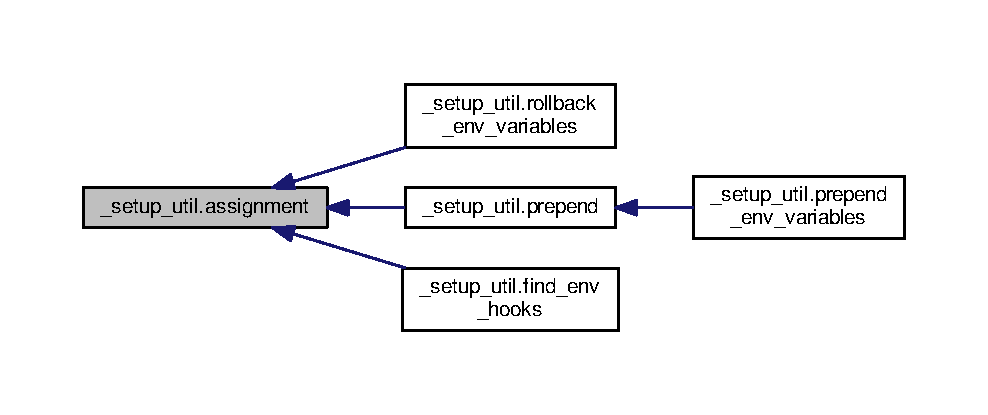
\includegraphics[width=350pt]{namespace__setup__util_ad56c24837fa4eddc63c03fbc7035628f_icgraph}
\end{center}
\end{figure}


\index{\+\_\+setup\+\_\+util@{\+\_\+setup\+\_\+util}!comment@{comment}}
\index{comment@{comment}!\+\_\+setup\+\_\+util@{\+\_\+setup\+\_\+util}}
\subsubsection[{\texorpdfstring{comment(msg)}{comment(msg)}}]{\setlength{\rightskip}{0pt plus 5cm}def \+\_\+setup\+\_\+util.\+comment (
\begin{DoxyParamCaption}
\item[{}]{msg}
\end{DoxyParamCaption}
)}\hypertarget{namespace__setup__util_abe8c95c4cfe8b1374dacd5f91d984353}{}\label{namespace__setup__util_abe8c95c4cfe8b1374dacd5f91d984353}


Definition at line 182 of file \+\_\+setup\+\_\+util.\+py.



Here is the caller graph for this function\+:
\nopagebreak
\begin{figure}[H]
\begin{center}
\leavevmode
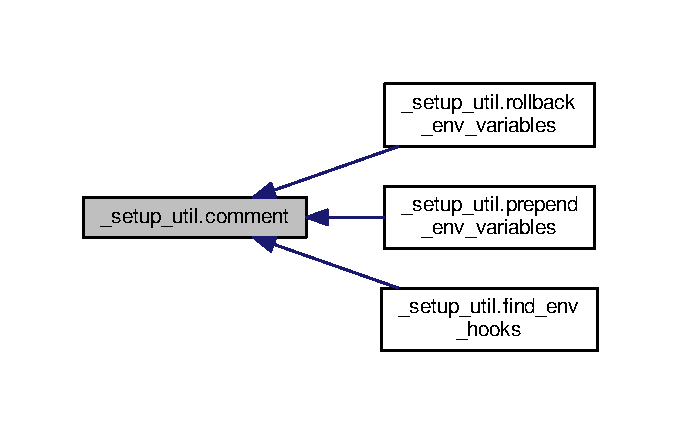
\includegraphics[width=327pt]{namespace__setup__util_abe8c95c4cfe8b1374dacd5f91d984353_icgraph}
\end{center}
\end{figure}


\index{\+\_\+setup\+\_\+util@{\+\_\+setup\+\_\+util}!find\+\_\+env\+\_\+hooks@{find\+\_\+env\+\_\+hooks}}
\index{find\+\_\+env\+\_\+hooks@{find\+\_\+env\+\_\+hooks}!\+\_\+setup\+\_\+util@{\+\_\+setup\+\_\+util}}
\subsubsection[{\texorpdfstring{find\+\_\+env\+\_\+hooks(environ, cmake\+\_\+prefix\+\_\+path)}{find_env_hooks(environ, cmake_prefix_path)}}]{\setlength{\rightskip}{0pt plus 5cm}def \+\_\+setup\+\_\+util.\+find\+\_\+env\+\_\+hooks (
\begin{DoxyParamCaption}
\item[{}]{environ, }
\item[{}]{cmake\+\_\+prefix\+\_\+path}
\end{DoxyParamCaption}
)}\hypertarget{namespace__setup__util_a73de35ca77f260af6691470342ab49ce}{}\label{namespace__setup__util_a73de35ca77f260af6691470342ab49ce}
\begin{DoxyVerb}Generate shell code with found environment hooks
for the all workspaces.
\end{DoxyVerb}
 

Definition at line 198 of file \+\_\+setup\+\_\+util.\+py.



Here is the call graph for this function\+:
\nopagebreak
\begin{figure}[H]
\begin{center}
\leavevmode
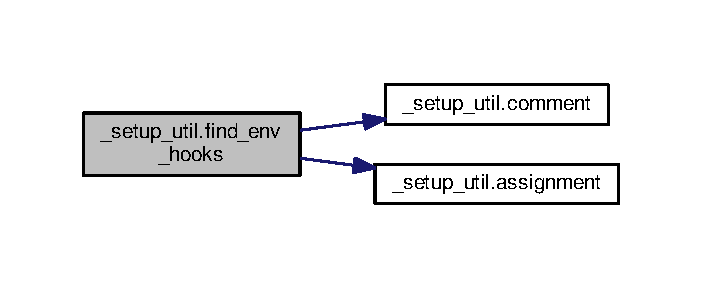
\includegraphics[width=337pt]{namespace__setup__util_a73de35ca77f260af6691470342ab49ce_cgraph}
\end{center}
\end{figure}


\index{\+\_\+setup\+\_\+util@{\+\_\+setup\+\_\+util}!prepend@{prepend}}
\index{prepend@{prepend}!\+\_\+setup\+\_\+util@{\+\_\+setup\+\_\+util}}
\subsubsection[{\texorpdfstring{prepend(environ, key, prefix)}{prepend(environ, key, prefix)}}]{\setlength{\rightskip}{0pt plus 5cm}def \+\_\+setup\+\_\+util.\+prepend (
\begin{DoxyParamCaption}
\item[{}]{environ, }
\item[{}]{key, }
\item[{}]{prefix}
\end{DoxyParamCaption}
)}\hypertarget{namespace__setup__util_ae78d86b2c4279f5b8b1acaa146c35802}{}\label{namespace__setup__util_ae78d86b2c4279f5b8b1acaa146c35802}


Definition at line 189 of file \+\_\+setup\+\_\+util.\+py.



Here is the call graph for this function\+:
\nopagebreak
\begin{figure}[H]
\begin{center}
\leavevmode
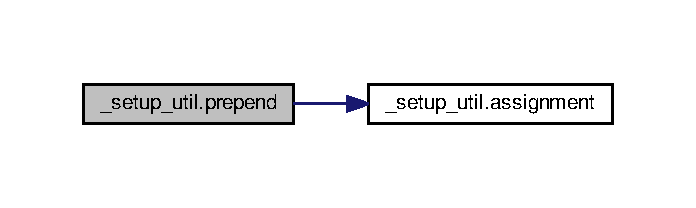
\includegraphics[width=334pt]{namespace__setup__util_ae78d86b2c4279f5b8b1acaa146c35802_cgraph}
\end{center}
\end{figure}




Here is the caller graph for this function\+:
\nopagebreak
\begin{figure}[H]
\begin{center}
\leavevmode
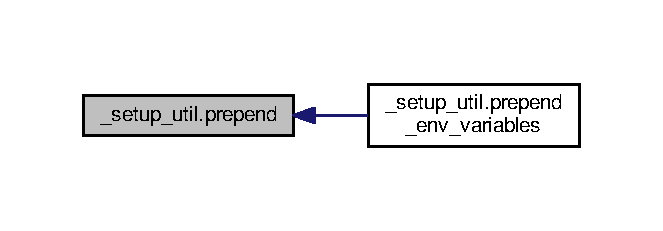
\includegraphics[width=318pt]{namespace__setup__util_ae78d86b2c4279f5b8b1acaa146c35802_icgraph}
\end{center}
\end{figure}


\index{\+\_\+setup\+\_\+util@{\+\_\+setup\+\_\+util}!prepend\+\_\+env\+\_\+variables@{prepend\+\_\+env\+\_\+variables}}
\index{prepend\+\_\+env\+\_\+variables@{prepend\+\_\+env\+\_\+variables}!\+\_\+setup\+\_\+util@{\+\_\+setup\+\_\+util}}
\subsubsection[{\texorpdfstring{prepend\+\_\+env\+\_\+variables(environ, env\+\_\+var\+\_\+subfolders, workspaces)}{prepend_env_variables(environ, env_var_subfolders, workspaces)}}]{\setlength{\rightskip}{0pt plus 5cm}def \+\_\+setup\+\_\+util.\+prepend\+\_\+env\+\_\+variables (
\begin{DoxyParamCaption}
\item[{}]{environ, }
\item[{}]{env\+\_\+var\+\_\+subfolders, }
\item[{}]{workspaces}
\end{DoxyParamCaption}
)}\hypertarget{namespace__setup__util_a832417d18b85bd1d276a87547e86f860}{}\label{namespace__setup__util_a832417d18b85bd1d276a87547e86f860}
\begin{DoxyVerb}Generate shell code to prepend environment variables
for the all workspaces.
\end{DoxyVerb}
 

Definition at line 129 of file \+\_\+setup\+\_\+util.\+py.



Here is the call graph for this function\+:
\nopagebreak
\begin{figure}[H]
\begin{center}
\leavevmode
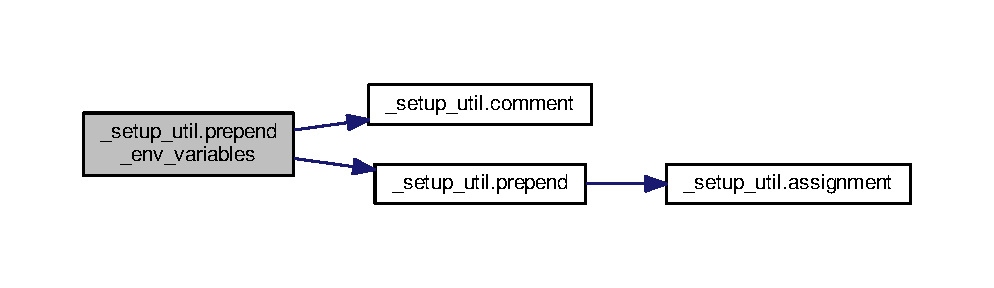
\includegraphics[width=350pt]{namespace__setup__util_a832417d18b85bd1d276a87547e86f860_cgraph}
\end{center}
\end{figure}


\index{\+\_\+setup\+\_\+util@{\+\_\+setup\+\_\+util}!rollback\+\_\+env\+\_\+variables@{rollback\+\_\+env\+\_\+variables}}
\index{rollback\+\_\+env\+\_\+variables@{rollback\+\_\+env\+\_\+variables}!\+\_\+setup\+\_\+util@{\+\_\+setup\+\_\+util}}
\subsubsection[{\texorpdfstring{rollback\+\_\+env\+\_\+variables(environ, env\+\_\+var\+\_\+subfolders)}{rollback_env_variables(environ, env_var_subfolders)}}]{\setlength{\rightskip}{0pt plus 5cm}def \+\_\+setup\+\_\+util.\+rollback\+\_\+env\+\_\+variables (
\begin{DoxyParamCaption}
\item[{}]{environ, }
\item[{}]{env\+\_\+var\+\_\+subfolders}
\end{DoxyParamCaption}
)}\hypertarget{namespace__setup__util_af3030db6102b5aa35cd354a2fb6cca03}{}\label{namespace__setup__util_af3030db6102b5aa35cd354a2fb6cca03}
\begin{DoxyVerb}Generate shell code to reset environment variables
by unrolling modifications based on all workspaces in CMAKE_PREFIX_PATH.
This does not cover modifications performed by environment hooks.
\end{DoxyVerb}
 

Definition at line 62 of file \+\_\+setup\+\_\+util.\+py.



Here is the call graph for this function\+:
\nopagebreak
\begin{figure}[H]
\begin{center}
\leavevmode
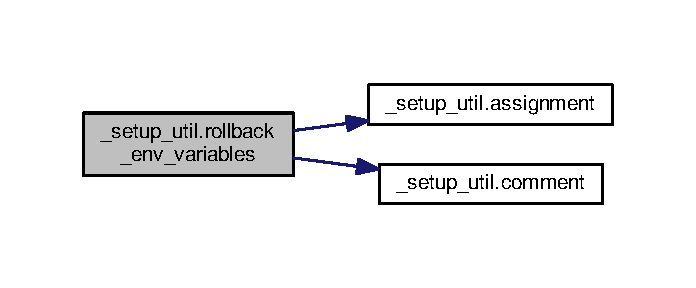
\includegraphics[width=334pt]{namespace__setup__util_af3030db6102b5aa35cd354a2fb6cca03_cgraph}
\end{center}
\end{figure}




\subsection{Variable Documentation}
\index{\+\_\+setup\+\_\+util@{\+\_\+setup\+\_\+util}!args@{args}}
\index{args@{args}!\+\_\+setup\+\_\+util@{\+\_\+setup\+\_\+util}}
\subsubsection[{\texorpdfstring{args}{args}}]{\setlength{\rightskip}{0pt plus 5cm}\+\_\+setup\+\_\+util.\+args = \+\_\+parse\+\_\+arguments()}\hypertarget{namespace__setup__util_a547963d07c6371df1c51b1384a2dec28}{}\label{namespace__setup__util_a547963d07c6371df1c51b1384a2dec28}


Definition at line 259 of file \+\_\+setup\+\_\+util.\+py.

\index{\+\_\+setup\+\_\+util@{\+\_\+setup\+\_\+util}!base\+\_\+path@{base\+\_\+path}}
\index{base\+\_\+path@{base\+\_\+path}!\+\_\+setup\+\_\+util@{\+\_\+setup\+\_\+util}}
\subsubsection[{\texorpdfstring{base\+\_\+path}{base_path}}]{\setlength{\rightskip}{0pt plus 5cm}\+\_\+setup\+\_\+util.\+base\+\_\+path = os.\+path.\+dirname(\+\_\+\+\_\+file\+\_\+\+\_\+)}\hypertarget{namespace__setup__util_a83d25140acd7788bbcb95843fe38e639}{}\label{namespace__setup__util_a83d25140acd7788bbcb95843fe38e639}


Definition at line 267 of file \+\_\+setup\+\_\+util.\+py.

\index{\+\_\+setup\+\_\+util@{\+\_\+setup\+\_\+util}!C\+A\+T\+K\+I\+N\+\_\+\+M\+A\+R\+K\+E\+R\+\_\+\+F\+I\+LE@{C\+A\+T\+K\+I\+N\+\_\+\+M\+A\+R\+K\+E\+R\+\_\+\+F\+I\+LE}}
\index{C\+A\+T\+K\+I\+N\+\_\+\+M\+A\+R\+K\+E\+R\+\_\+\+F\+I\+LE@{C\+A\+T\+K\+I\+N\+\_\+\+M\+A\+R\+K\+E\+R\+\_\+\+F\+I\+LE}!\+\_\+setup\+\_\+util@{\+\_\+setup\+\_\+util}}
\subsubsection[{\texorpdfstring{C\+A\+T\+K\+I\+N\+\_\+\+M\+A\+R\+K\+E\+R\+\_\+\+F\+I\+LE}{CATKIN_MARKER_FILE}}]{\setlength{\rightskip}{0pt plus 5cm}string \+\_\+setup\+\_\+util.\+C\+A\+T\+K\+I\+N\+\_\+\+M\+A\+R\+K\+E\+R\+\_\+\+F\+I\+LE = \textquotesingle{}.catkin\textquotesingle{}}\hypertarget{namespace__setup__util_a3fa0ca5a460a71a43cbc3d4954ab1f10}{}\label{namespace__setup__util_a3fa0ca5a460a71a43cbc3d4954ab1f10}


Definition at line 46 of file \+\_\+setup\+\_\+util.\+py.

\index{\+\_\+setup\+\_\+util@{\+\_\+setup\+\_\+util}!C\+M\+A\+K\+E\+\_\+\+P\+R\+E\+F\+I\+X\+\_\+\+P\+A\+TH@{C\+M\+A\+K\+E\+\_\+\+P\+R\+E\+F\+I\+X\+\_\+\+P\+A\+TH}}
\index{C\+M\+A\+K\+E\+\_\+\+P\+R\+E\+F\+I\+X\+\_\+\+P\+A\+TH@{C\+M\+A\+K\+E\+\_\+\+P\+R\+E\+F\+I\+X\+\_\+\+P\+A\+TH}!\+\_\+setup\+\_\+util@{\+\_\+setup\+\_\+util}}
\subsubsection[{\texorpdfstring{C\+M\+A\+K\+E\+\_\+\+P\+R\+E\+F\+I\+X\+\_\+\+P\+A\+TH}{CMAKE_PREFIX_PATH}}]{\setlength{\rightskip}{0pt plus 5cm}string \+\_\+setup\+\_\+util.\+C\+M\+A\+K\+E\+\_\+\+P\+R\+E\+F\+I\+X\+\_\+\+P\+A\+TH = \textquotesingle{}/home/jbs/catkin\+\_\+ws/devel;/opt/ros/kinetic\textquotesingle{}}\hypertarget{namespace__setup__util_a57afd3d2c076955fb715f3e72ef098eb}{}\label{namespace__setup__util_a57afd3d2c076955fb715f3e72ef098eb}


Definition at line 265 of file \+\_\+setup\+\_\+util.\+py.

\index{\+\_\+setup\+\_\+util@{\+\_\+setup\+\_\+util}!e@{e}}
\index{e@{e}!\+\_\+setup\+\_\+util@{\+\_\+setup\+\_\+util}}
\subsubsection[{\texorpdfstring{e}{e}}]{\setlength{\rightskip}{0pt plus 5cm}\+\_\+setup\+\_\+util.\+e}\hypertarget{namespace__setup__util_acdce690b925de33d6249bbbfa1109d61}{}\label{namespace__setup__util_acdce690b925de33d6249bbbfa1109d61}


Definition at line 261 of file \+\_\+setup\+\_\+util.\+py.

\index{\+\_\+setup\+\_\+util@{\+\_\+setup\+\_\+util}!E\+N\+V\+\_\+\+V\+A\+R\+\_\+\+S\+U\+B\+F\+O\+L\+D\+E\+RS@{E\+N\+V\+\_\+\+V\+A\+R\+\_\+\+S\+U\+B\+F\+O\+L\+D\+E\+RS}}
\index{E\+N\+V\+\_\+\+V\+A\+R\+\_\+\+S\+U\+B\+F\+O\+L\+D\+E\+RS@{E\+N\+V\+\_\+\+V\+A\+R\+\_\+\+S\+U\+B\+F\+O\+L\+D\+E\+RS}!\+\_\+setup\+\_\+util@{\+\_\+setup\+\_\+util}}
\subsubsection[{\texorpdfstring{E\+N\+V\+\_\+\+V\+A\+R\+\_\+\+S\+U\+B\+F\+O\+L\+D\+E\+RS}{ENV_VAR_SUBFOLDERS}}]{\setlength{\rightskip}{0pt plus 5cm}dictionary \+\_\+setup\+\_\+util.\+E\+N\+V\+\_\+\+V\+A\+R\+\_\+\+S\+U\+B\+F\+O\+L\+D\+E\+RS}\hypertarget{namespace__setup__util_aa31804f1be8660156ce9394b33c68dc4}{}\label{namespace__setup__util_aa31804f1be8660156ce9394b33c68dc4}
{\bfseries Initial value\+:}
\begin{DoxyCode}
1 = \{
2     \textcolor{stringliteral}{'CMAKE\_PREFIX\_PATH'}: \textcolor{stringliteral}{''},
3     \textcolor{stringliteral}{'LD\_LIBRARY\_PATH'} \textcolor{keywordflow}{if} \textcolor{keywordflow}{not} IS\_DARWIN \textcolor{keywordflow}{else} \textcolor{stringliteral}{'DYLD\_LIBRARY\_PATH'}: [\textcolor{stringliteral}{'lib'}, os.path.join(\textcolor{stringliteral}{'lib'}, \textcolor{stringliteral}{'
      x86\_64-linux-gnu'})],
4     \textcolor{stringliteral}{'PATH'}: \textcolor{stringliteral}{'bin'},
5     \textcolor{stringliteral}{'PKG\_CONFIG\_PATH'}: [os.path.join(\textcolor{stringliteral}{'lib'}, \textcolor{stringliteral}{'pkgconfig'}), os.path.join(\textcolor{stringliteral}{'lib'}, \textcolor{stringliteral}{'x86\_64-linux-gnu'}, \textcolor{stringliteral}{'
      pkgconfig'})],
6     \textcolor{stringliteral}{'PYTHONPATH'}: \textcolor{stringliteral}{'lib/python2.7/dist-packages'},
7 \}
\end{DoxyCode}


Definition at line 53 of file \+\_\+setup\+\_\+util.\+py.

\index{\+\_\+setup\+\_\+util@{\+\_\+setup\+\_\+util}!environ@{environ}}
\index{environ@{environ}!\+\_\+setup\+\_\+util@{\+\_\+setup\+\_\+util}}
\subsubsection[{\texorpdfstring{environ}{environ}}]{\setlength{\rightskip}{0pt plus 5cm}\+\_\+setup\+\_\+util.\+environ = dict(os.\+environ)}\hypertarget{namespace__setup__util_a9a935bdd9ee1aa0327161025bb18c136}{}\label{namespace__setup__util_a9a935bdd9ee1aa0327161025bb18c136}


Definition at line 272 of file \+\_\+setup\+\_\+util.\+py.

\index{\+\_\+setup\+\_\+util@{\+\_\+setup\+\_\+util}!file@{file}}
\index{file@{file}!\+\_\+setup\+\_\+util@{\+\_\+setup\+\_\+util}}
\subsubsection[{\texorpdfstring{file}{file}}]{\setlength{\rightskip}{0pt plus 5cm}\+\_\+setup\+\_\+util.\+file}\hypertarget{namespace__setup__util_aea63a1b32cc79bc3d872ab7cb30dd07e}{}\label{namespace__setup__util_aea63a1b32cc79bc3d872ab7cb30dd07e}


Definition at line 261 of file \+\_\+setup\+\_\+util.\+py.

\index{\+\_\+setup\+\_\+util@{\+\_\+setup\+\_\+util}!I\+S\+\_\+\+D\+A\+R\+W\+IN@{I\+S\+\_\+\+D\+A\+R\+W\+IN}}
\index{I\+S\+\_\+\+D\+A\+R\+W\+IN@{I\+S\+\_\+\+D\+A\+R\+W\+IN}!\+\_\+setup\+\_\+util@{\+\_\+setup\+\_\+util}}
\subsubsection[{\texorpdfstring{I\+S\+\_\+\+D\+A\+R\+W\+IN}{IS_DARWIN}}]{\setlength{\rightskip}{0pt plus 5cm}tuple \+\_\+setup\+\_\+util.\+I\+S\+\_\+\+D\+A\+R\+W\+IN = ({\bf system} == \textquotesingle{}Darwin\textquotesingle{})}\hypertarget{namespace__setup__util_aecbb100ce6f94bb3c7e16d58fde05f96}{}\label{namespace__setup__util_aecbb100ce6f94bb3c7e16d58fde05f96}


Definition at line 49 of file \+\_\+setup\+\_\+util.\+py.

\index{\+\_\+setup\+\_\+util@{\+\_\+setup\+\_\+util}!I\+S\+\_\+\+W\+I\+N\+D\+O\+WS@{I\+S\+\_\+\+W\+I\+N\+D\+O\+WS}}
\index{I\+S\+\_\+\+W\+I\+N\+D\+O\+WS@{I\+S\+\_\+\+W\+I\+N\+D\+O\+WS}!\+\_\+setup\+\_\+util@{\+\_\+setup\+\_\+util}}
\subsubsection[{\texorpdfstring{I\+S\+\_\+\+W\+I\+N\+D\+O\+WS}{IS_WINDOWS}}]{\setlength{\rightskip}{0pt plus 5cm}tuple \+\_\+setup\+\_\+util.\+I\+S\+\_\+\+W\+I\+N\+D\+O\+WS = ({\bf system} == \textquotesingle{}Windows\textquotesingle{})}\hypertarget{namespace__setup__util_a6fe69c2dbd92959b6651a28cbb846e6e}{}\label{namespace__setup__util_a6fe69c2dbd92959b6651a28cbb846e6e}


Definition at line 50 of file \+\_\+setup\+\_\+util.\+py.

\index{\+\_\+setup\+\_\+util@{\+\_\+setup\+\_\+util}!lines@{lines}}
\index{lines@{lines}!\+\_\+setup\+\_\+util@{\+\_\+setup\+\_\+util}}
\subsubsection[{\texorpdfstring{lines}{lines}}]{\setlength{\rightskip}{0pt plus 5cm}list \+\_\+setup\+\_\+util.\+lines = \mbox{[}$\,$\mbox{]}}\hypertarget{namespace__setup__util_a8618d8be5f729d4c9696daa5e083a001}{}\label{namespace__setup__util_a8618d8be5f729d4c9696daa5e083a001}


Definition at line 273 of file \+\_\+setup\+\_\+util.\+py.

\index{\+\_\+setup\+\_\+util@{\+\_\+setup\+\_\+util}!system@{system}}
\index{system@{system}!\+\_\+setup\+\_\+util@{\+\_\+setup\+\_\+util}}
\subsubsection[{\texorpdfstring{system}{system}}]{\setlength{\rightskip}{0pt plus 5cm}\+\_\+setup\+\_\+util.\+system = platform.\+system()}\hypertarget{namespace__setup__util_ae9fca6a80a6923f4580be72f68fee325}{}\label{namespace__setup__util_ae9fca6a80a6923f4580be72f68fee325}


Definition at line 48 of file \+\_\+setup\+\_\+util.\+py.


\hypertarget{namespacegenerate__cached__setup}{}\section{generate\+\_\+cached\+\_\+setup Namespace Reference}
\label{namespacegenerate__cached__setup}\index{generate\+\_\+cached\+\_\+setup@{generate\+\_\+cached\+\_\+setup}}
\subsection*{Variables}
\begin{DoxyCompactItemize}
\item 
\hyperlink{namespacegenerate__cached__setup_a72579fd01529a79bab20d99291889d3f}{python\+\_\+path} = os.\+path.\+join(workspace, \textquotesingle{}lib/python2.\+7/dist-\/packages\textquotesingle{})
\item 
\hyperlink{namespacegenerate__cached__setup_a52601295006f2366a311c4453d8f2f2e}{code} = generate\+\_\+environment\+\_\+script(\textquotesingle{}/home/jbs/catkin\+\_\+ws/src/traj\+\_\+gen/build/devel/env.\+sh\textquotesingle{})
\item 
string \hyperlink{namespacegenerate__cached__setup_a0265aee5075ee1eb701ff69c98ad6793}{output\+\_\+filename} = \textquotesingle{}/home/jbs/catkin\+\_\+ws/src/traj\+\_\+gen/build/catkin\+\_\+generated/setup\+\_\+cached.\+sh\textquotesingle{}
\item 
\hyperlink{namespacegenerate__cached__setup_a10081e5abedae9bd46dd91202096e789}{mode} = os.\+stat(\hyperlink{namespacegenerate__cached__setup_a0265aee5075ee1eb701ff69c98ad6793}{output\+\_\+filename}).st\+\_\+mode
\end{DoxyCompactItemize}


\subsection{Variable Documentation}
\index{generate\+\_\+cached\+\_\+setup@{generate\+\_\+cached\+\_\+setup}!code@{code}}
\index{code@{code}!generate\+\_\+cached\+\_\+setup@{generate\+\_\+cached\+\_\+setup}}
\subsubsection[{\texorpdfstring{code}{code}}]{\setlength{\rightskip}{0pt plus 5cm}generate\+\_\+cached\+\_\+setup.\+code = generate\+\_\+environment\+\_\+script(\textquotesingle{}/home/jbs/catkin\+\_\+ws/src/traj\+\_\+gen/build/devel/env.\+sh\textquotesingle{})}\hypertarget{namespacegenerate__cached__setup_a52601295006f2366a311c4453d8f2f2e}{}\label{namespacegenerate__cached__setup_a52601295006f2366a311c4453d8f2f2e}


Definition at line 22 of file generate\+\_\+cached\+\_\+setup.\+py.

\index{generate\+\_\+cached\+\_\+setup@{generate\+\_\+cached\+\_\+setup}!mode@{mode}}
\index{mode@{mode}!generate\+\_\+cached\+\_\+setup@{generate\+\_\+cached\+\_\+setup}}
\subsubsection[{\texorpdfstring{mode}{mode}}]{\setlength{\rightskip}{0pt plus 5cm}generate\+\_\+cached\+\_\+setup.\+mode = os.\+stat({\bf output\+\_\+filename}).st\+\_\+mode}\hypertarget{namespacegenerate__cached__setup_a10081e5abedae9bd46dd91202096e789}{}\label{namespacegenerate__cached__setup_a10081e5abedae9bd46dd91202096e789}


Definition at line 29 of file generate\+\_\+cached\+\_\+setup.\+py.

\index{generate\+\_\+cached\+\_\+setup@{generate\+\_\+cached\+\_\+setup}!output\+\_\+filename@{output\+\_\+filename}}
\index{output\+\_\+filename@{output\+\_\+filename}!generate\+\_\+cached\+\_\+setup@{generate\+\_\+cached\+\_\+setup}}
\subsubsection[{\texorpdfstring{output\+\_\+filename}{output_filename}}]{\setlength{\rightskip}{0pt plus 5cm}string generate\+\_\+cached\+\_\+setup.\+output\+\_\+filename = \textquotesingle{}/home/jbs/catkin\+\_\+ws/src/traj\+\_\+gen/build/catkin\+\_\+generated/setup\+\_\+cached.\+sh\textquotesingle{}}\hypertarget{namespacegenerate__cached__setup_a0265aee5075ee1eb701ff69c98ad6793}{}\label{namespacegenerate__cached__setup_a0265aee5075ee1eb701ff69c98ad6793}


Definition at line 24 of file generate\+\_\+cached\+\_\+setup.\+py.

\index{generate\+\_\+cached\+\_\+setup@{generate\+\_\+cached\+\_\+setup}!python\+\_\+path@{python\+\_\+path}}
\index{python\+\_\+path@{python\+\_\+path}!generate\+\_\+cached\+\_\+setup@{generate\+\_\+cached\+\_\+setup}}
\subsubsection[{\texorpdfstring{python\+\_\+path}{python_path}}]{\setlength{\rightskip}{0pt plus 5cm}generate\+\_\+cached\+\_\+setup.\+python\+\_\+path = os.\+path.\+join(workspace, \textquotesingle{}lib/python2.\+7/dist-\/packages\textquotesingle{})}\hypertarget{namespacegenerate__cached__setup_a72579fd01529a79bab20d99291889d3f}{}\label{namespacegenerate__cached__setup_a72579fd01529a79bab20d99291889d3f}


Definition at line 16 of file generate\+\_\+cached\+\_\+setup.\+py.


\hypertarget{namespacepkg}{}\section{pkg Namespace Reference}
\label{namespacepkg}\index{pkg@{pkg}}
\subsection*{Variables}
\begin{DoxyCompactItemize}
\item 
string \hyperlink{namespacepkg_ae26c7a5a06b7d738f4d210ca449e6bee}{C\+A\+T\+K\+I\+N\+\_\+\+P\+A\+C\+K\+A\+G\+E\+\_\+\+P\+R\+E\+F\+IX} = \char`\"{}\char`\"{}
\item 
string \hyperlink{namespacepkg_a2760bf8266ff58da440f65ee91b203ab}{P\+R\+O\+J\+E\+C\+T\+\_\+\+P\+K\+G\+\_\+\+C\+O\+N\+F\+I\+G\+\_\+\+I\+N\+C\+L\+U\+D\+E\+\_\+\+D\+I\+RS} = \char`\"{}/home/jbs/catkin\+\_\+ws/src/traj\+\_\+gen/build/devel/include;/home/jbs/catkin\+\_\+ws/src/traj\+\_\+gen/include\char`\"{}
\item 
string \hyperlink{namespacepkg_a17c18447fad253ee1c0d76deec88028c}{P\+R\+O\+J\+E\+C\+T\+\_\+\+C\+A\+T\+K\+I\+N\+\_\+\+D\+E\+P\+E\+N\+DS} = \char`\"{}message\+\_\+generation;\hyperlink{_spline_gen_8js_a1fa5a20fd50395f7b988c134be2a3d32}{nav\+\_\+msgs};roscpp\char`\"{}
\item 
string \hyperlink{namespacepkg_a433e30cecb4a0123a7c4b384d168e336}{P\+K\+G\+\_\+\+C\+O\+N\+F\+I\+G\+\_\+\+L\+I\+B\+R\+A\+R\+I\+E\+S\+\_\+\+W\+I\+T\+H\+\_\+\+P\+R\+E\+F\+IX} = \char`\"{}-\/ltraj\+\_\+gen\char`\"{}
\item 
string \hyperlink{namespacepkg_a7dfbe99257c26f5e4a3a5483995d9ddc}{P\+R\+O\+J\+E\+C\+T\+\_\+\+N\+A\+ME} = \char`\"{}traj\+\_\+gen\char`\"{}
\item 
string \hyperlink{namespacepkg_a3f0f1b4bc03c596525e025539ca4332f}{P\+R\+O\+J\+E\+C\+T\+\_\+\+S\+P\+A\+C\+E\+\_\+\+D\+IR} = \char`\"{}/home/jbs/catkin\+\_\+ws/src/traj\+\_\+gen/build/devel\char`\"{}
\item 
string \hyperlink{namespacepkg_ab1037914b9286bb61855131c06149648}{P\+R\+O\+J\+E\+C\+T\+\_\+\+V\+E\+R\+S\+I\+ON} = \char`\"{}0.\+0.\+0\char`\"{}
\end{DoxyCompactItemize}


\subsection{Variable Documentation}
\index{pkg@{pkg}!C\+A\+T\+K\+I\+N\+\_\+\+P\+A\+C\+K\+A\+G\+E\+\_\+\+P\+R\+E\+F\+IX@{C\+A\+T\+K\+I\+N\+\_\+\+P\+A\+C\+K\+A\+G\+E\+\_\+\+P\+R\+E\+F\+IX}}
\index{C\+A\+T\+K\+I\+N\+\_\+\+P\+A\+C\+K\+A\+G\+E\+\_\+\+P\+R\+E\+F\+IX@{C\+A\+T\+K\+I\+N\+\_\+\+P\+A\+C\+K\+A\+G\+E\+\_\+\+P\+R\+E\+F\+IX}!pkg@{pkg}}
\subsubsection[{\texorpdfstring{C\+A\+T\+K\+I\+N\+\_\+\+P\+A\+C\+K\+A\+G\+E\+\_\+\+P\+R\+E\+F\+IX}{CATKIN_PACKAGE_PREFIX}}]{\setlength{\rightskip}{0pt plus 5cm}string pkg.\+C\+A\+T\+K\+I\+N\+\_\+\+P\+A\+C\+K\+A\+G\+E\+\_\+\+P\+R\+E\+F\+IX = \char`\"{}\char`\"{}}\hypertarget{namespacepkg_ae26c7a5a06b7d738f4d210ca449e6bee}{}\label{namespacepkg_ae26c7a5a06b7d738f4d210ca449e6bee}


Definition at line 2 of file pkg.\+develspace.\+context.\+pc.\+py.

\index{pkg@{pkg}!P\+K\+G\+\_\+\+C\+O\+N\+F\+I\+G\+\_\+\+L\+I\+B\+R\+A\+R\+I\+E\+S\+\_\+\+W\+I\+T\+H\+\_\+\+P\+R\+E\+F\+IX@{P\+K\+G\+\_\+\+C\+O\+N\+F\+I\+G\+\_\+\+L\+I\+B\+R\+A\+R\+I\+E\+S\+\_\+\+W\+I\+T\+H\+\_\+\+P\+R\+E\+F\+IX}}
\index{P\+K\+G\+\_\+\+C\+O\+N\+F\+I\+G\+\_\+\+L\+I\+B\+R\+A\+R\+I\+E\+S\+\_\+\+W\+I\+T\+H\+\_\+\+P\+R\+E\+F\+IX@{P\+K\+G\+\_\+\+C\+O\+N\+F\+I\+G\+\_\+\+L\+I\+B\+R\+A\+R\+I\+E\+S\+\_\+\+W\+I\+T\+H\+\_\+\+P\+R\+E\+F\+IX}!pkg@{pkg}}
\subsubsection[{\texorpdfstring{P\+K\+G\+\_\+\+C\+O\+N\+F\+I\+G\+\_\+\+L\+I\+B\+R\+A\+R\+I\+E\+S\+\_\+\+W\+I\+T\+H\+\_\+\+P\+R\+E\+F\+IX}{PKG_CONFIG_LIBRARIES_WITH_PREFIX}}]{\setlength{\rightskip}{0pt plus 5cm}string pkg.\+P\+K\+G\+\_\+\+C\+O\+N\+F\+I\+G\+\_\+\+L\+I\+B\+R\+A\+R\+I\+E\+S\+\_\+\+W\+I\+T\+H\+\_\+\+P\+R\+E\+F\+IX = \char`\"{}-\/ltraj\+\_\+gen\char`\"{}}\hypertarget{namespacepkg_a433e30cecb4a0123a7c4b384d168e336}{}\label{namespacepkg_a433e30cecb4a0123a7c4b384d168e336}


Definition at line 5 of file pkg.\+develspace.\+context.\+pc.\+py.

\index{pkg@{pkg}!P\+R\+O\+J\+E\+C\+T\+\_\+\+C\+A\+T\+K\+I\+N\+\_\+\+D\+E\+P\+E\+N\+DS@{P\+R\+O\+J\+E\+C\+T\+\_\+\+C\+A\+T\+K\+I\+N\+\_\+\+D\+E\+P\+E\+N\+DS}}
\index{P\+R\+O\+J\+E\+C\+T\+\_\+\+C\+A\+T\+K\+I\+N\+\_\+\+D\+E\+P\+E\+N\+DS@{P\+R\+O\+J\+E\+C\+T\+\_\+\+C\+A\+T\+K\+I\+N\+\_\+\+D\+E\+P\+E\+N\+DS}!pkg@{pkg}}
\subsubsection[{\texorpdfstring{P\+R\+O\+J\+E\+C\+T\+\_\+\+C\+A\+T\+K\+I\+N\+\_\+\+D\+E\+P\+E\+N\+DS}{PROJECT_CATKIN_DEPENDS}}]{\setlength{\rightskip}{0pt plus 5cm}string pkg.\+P\+R\+O\+J\+E\+C\+T\+\_\+\+C\+A\+T\+K\+I\+N\+\_\+\+D\+E\+P\+E\+N\+DS = \char`\"{}message\+\_\+generation;{\bf nav\+\_\+msgs};roscpp\char`\"{}}\hypertarget{namespacepkg_a17c18447fad253ee1c0d76deec88028c}{}\label{namespacepkg_a17c18447fad253ee1c0d76deec88028c}


Definition at line 4 of file pkg.\+develspace.\+context.\+pc.\+py.

\index{pkg@{pkg}!P\+R\+O\+J\+E\+C\+T\+\_\+\+N\+A\+ME@{P\+R\+O\+J\+E\+C\+T\+\_\+\+N\+A\+ME}}
\index{P\+R\+O\+J\+E\+C\+T\+\_\+\+N\+A\+ME@{P\+R\+O\+J\+E\+C\+T\+\_\+\+N\+A\+ME}!pkg@{pkg}}
\subsubsection[{\texorpdfstring{P\+R\+O\+J\+E\+C\+T\+\_\+\+N\+A\+ME}{PROJECT_NAME}}]{\setlength{\rightskip}{0pt plus 5cm}string pkg.\+P\+R\+O\+J\+E\+C\+T\+\_\+\+N\+A\+ME = \char`\"{}traj\+\_\+gen\char`\"{}}\hypertarget{namespacepkg_a7dfbe99257c26f5e4a3a5483995d9ddc}{}\label{namespacepkg_a7dfbe99257c26f5e4a3a5483995d9ddc}


Definition at line 6 of file pkg.\+develspace.\+context.\+pc.\+py.

\index{pkg@{pkg}!P\+R\+O\+J\+E\+C\+T\+\_\+\+P\+K\+G\+\_\+\+C\+O\+N\+F\+I\+G\+\_\+\+I\+N\+C\+L\+U\+D\+E\+\_\+\+D\+I\+RS@{P\+R\+O\+J\+E\+C\+T\+\_\+\+P\+K\+G\+\_\+\+C\+O\+N\+F\+I\+G\+\_\+\+I\+N\+C\+L\+U\+D\+E\+\_\+\+D\+I\+RS}}
\index{P\+R\+O\+J\+E\+C\+T\+\_\+\+P\+K\+G\+\_\+\+C\+O\+N\+F\+I\+G\+\_\+\+I\+N\+C\+L\+U\+D\+E\+\_\+\+D\+I\+RS@{P\+R\+O\+J\+E\+C\+T\+\_\+\+P\+K\+G\+\_\+\+C\+O\+N\+F\+I\+G\+\_\+\+I\+N\+C\+L\+U\+D\+E\+\_\+\+D\+I\+RS}!pkg@{pkg}}
\subsubsection[{\texorpdfstring{P\+R\+O\+J\+E\+C\+T\+\_\+\+P\+K\+G\+\_\+\+C\+O\+N\+F\+I\+G\+\_\+\+I\+N\+C\+L\+U\+D\+E\+\_\+\+D\+I\+RS}{PROJECT_PKG_CONFIG_INCLUDE_DIRS}}]{\setlength{\rightskip}{0pt plus 5cm}string pkg.\+P\+R\+O\+J\+E\+C\+T\+\_\+\+P\+K\+G\+\_\+\+C\+O\+N\+F\+I\+G\+\_\+\+I\+N\+C\+L\+U\+D\+E\+\_\+\+D\+I\+RS = \char`\"{}/home/jbs/catkin\+\_\+ws/src/traj\+\_\+gen/build/devel/include;/home/jbs/catkin\+\_\+ws/src/traj\+\_\+gen/include\char`\"{}}\hypertarget{namespacepkg_a2760bf8266ff58da440f65ee91b203ab}{}\label{namespacepkg_a2760bf8266ff58da440f65ee91b203ab}


Definition at line 3 of file pkg.\+develspace.\+context.\+pc.\+py.

\index{pkg@{pkg}!P\+R\+O\+J\+E\+C\+T\+\_\+\+S\+P\+A\+C\+E\+\_\+\+D\+IR@{P\+R\+O\+J\+E\+C\+T\+\_\+\+S\+P\+A\+C\+E\+\_\+\+D\+IR}}
\index{P\+R\+O\+J\+E\+C\+T\+\_\+\+S\+P\+A\+C\+E\+\_\+\+D\+IR@{P\+R\+O\+J\+E\+C\+T\+\_\+\+S\+P\+A\+C\+E\+\_\+\+D\+IR}!pkg@{pkg}}
\subsubsection[{\texorpdfstring{P\+R\+O\+J\+E\+C\+T\+\_\+\+S\+P\+A\+C\+E\+\_\+\+D\+IR}{PROJECT_SPACE_DIR}}]{\setlength{\rightskip}{0pt plus 5cm}string pkg.\+P\+R\+O\+J\+E\+C\+T\+\_\+\+S\+P\+A\+C\+E\+\_\+\+D\+IR = \char`\"{}/home/jbs/catkin\+\_\+ws/src/traj\+\_\+gen/build/devel\char`\"{}}\hypertarget{namespacepkg_a3f0f1b4bc03c596525e025539ca4332f}{}\label{namespacepkg_a3f0f1b4bc03c596525e025539ca4332f}


Definition at line 7 of file pkg.\+develspace.\+context.\+pc.\+py.

\index{pkg@{pkg}!P\+R\+O\+J\+E\+C\+T\+\_\+\+V\+E\+R\+S\+I\+ON@{P\+R\+O\+J\+E\+C\+T\+\_\+\+V\+E\+R\+S\+I\+ON}}
\index{P\+R\+O\+J\+E\+C\+T\+\_\+\+V\+E\+R\+S\+I\+ON@{P\+R\+O\+J\+E\+C\+T\+\_\+\+V\+E\+R\+S\+I\+ON}!pkg@{pkg}}
\subsubsection[{\texorpdfstring{P\+R\+O\+J\+E\+C\+T\+\_\+\+V\+E\+R\+S\+I\+ON}{PROJECT_VERSION}}]{\setlength{\rightskip}{0pt plus 5cm}string pkg.\+P\+R\+O\+J\+E\+C\+T\+\_\+\+V\+E\+R\+S\+I\+ON = \char`\"{}0.\+0.\+0\char`\"{}}\hypertarget{namespacepkg_ab1037914b9286bb61855131c06149648}{}\label{namespacepkg_ab1037914b9286bb61855131c06149648}


Definition at line 8 of file pkg.\+develspace.\+context.\+pc.\+py.


\hypertarget{namespaceros}{}\section{ros Namespace Reference}
\label{namespaceros}\index{ros@{ros}}
\subsection*{Namespaces}
\begin{DoxyCompactItemize}
\item 
 \hyperlink{namespaceros_1_1message__operations}{message\+\_\+operations}
\item 
 \hyperlink{namespaceros_1_1message__traits}{message\+\_\+traits}
\item 
 \hyperlink{namespaceros_1_1serialization}{serialization}
\item 
 \hyperlink{namespaceros_1_1service__traits}{service\+\_\+traits}
\end{DoxyCompactItemize}

\hypertarget{namespaceros_1_1message__operations}{}\section{ros\+:\+:message\+\_\+operations Namespace Reference}
\label{namespaceros_1_1message__operations}\index{ros\+::message\+\_\+operations@{ros\+::message\+\_\+operations}}
\subsection*{Classes}
\begin{DoxyCompactItemize}
\item 
struct \hyperlink{structros_1_1message__operations_1_1_printer_3_01_1_1traj__gen_1_1_poly_coeff___3_01_container_allocator_01_4_01_4}{Printer$<$ \+::traj\+\_\+gen\+::\+Poly\+Coeff\+\_\+$<$ Container\+Allocator $>$ $>$}
\item 
struct \hyperlink{structros_1_1message__operations_1_1_printer_3_01_1_1traj__gen_1_1_poly_spline___3_01_container_allocator_01_4_01_4}{Printer$<$ \+::traj\+\_\+gen\+::\+Poly\+Spline\+\_\+$<$ Container\+Allocator $>$ $>$}
\item 
struct \hyperlink{structros_1_1message__operations_1_1_printer_3_01_1_1traj__gen_1_1_poly_spline_x_y_z___3_01_container_allocator_01_4_01_4}{Printer$<$ \+::traj\+\_\+gen\+::\+Poly\+Spline\+X\+Y\+Z\+\_\+$<$ Container\+Allocator $>$ $>$}
\item 
struct \hyperlink{structros_1_1message__operations_1_1_printer_3_01_1_1traj__gen_1_1_spline_gen_request___3_01_container_allocator_01_4_01_4}{Printer$<$ \+::traj\+\_\+gen\+::\+Spline\+Gen\+Request\+\_\+$<$ Container\+Allocator $>$ $>$}
\item 
struct \hyperlink{structros_1_1message__operations_1_1_printer_3_01_1_1traj__gen_1_1_spline_gen_response___3_01_container_allocator_01_4_01_4}{Printer$<$ \+::traj\+\_\+gen\+::\+Spline\+Gen\+Response\+\_\+$<$ Container\+Allocator $>$ $>$}
\end{DoxyCompactItemize}

\hypertarget{namespaceros_1_1message__traits}{}\section{ros\+:\+:message\+\_\+traits Namespace Reference}
\label{namespaceros_1_1message__traits}\index{ros\+::message\+\_\+traits@{ros\+::message\+\_\+traits}}
\subsection*{Classes}
\begin{DoxyCompactItemize}
\item 
struct \hyperlink{structros_1_1message__traits_1_1_data_type_3_01_1_1traj__gen_1_1_poly_coeff___3_01_container_allocator_01_4_01_4}{Data\+Type$<$ \+::traj\+\_\+gen\+::\+Poly\+Coeff\+\_\+$<$ Container\+Allocator $>$ $>$}
\item 
struct \hyperlink{structros_1_1message__traits_1_1_data_type_3_01_1_1traj__gen_1_1_poly_spline___3_01_container_allocator_01_4_01_4}{Data\+Type$<$ \+::traj\+\_\+gen\+::\+Poly\+Spline\+\_\+$<$ Container\+Allocator $>$ $>$}
\item 
struct \hyperlink{structros_1_1message__traits_1_1_data_type_3_01_1_1traj__gen_1_1_poly_spline_x_y_z___3_01_container_allocator_01_4_01_4}{Data\+Type$<$ \+::traj\+\_\+gen\+::\+Poly\+Spline\+X\+Y\+Z\+\_\+$<$ Container\+Allocator $>$ $>$}
\item 
struct \hyperlink{structros_1_1message__traits_1_1_data_type_3_01_1_1traj__gen_1_1_spline_gen_request___3_01_container_allocator_01_4_01_4}{Data\+Type$<$ \+::traj\+\_\+gen\+::\+Spline\+Gen\+Request\+\_\+$<$ Container\+Allocator $>$ $>$}
\item 
struct \hyperlink{structros_1_1message__traits_1_1_data_type_3_01_1_1traj__gen_1_1_spline_gen_response___3_01_container_allocator_01_4_01_4}{Data\+Type$<$ \+::traj\+\_\+gen\+::\+Spline\+Gen\+Response\+\_\+$<$ Container\+Allocator $>$ $>$}
\item 
struct \hyperlink{structros_1_1message__traits_1_1_definition_3_01_1_1traj__gen_1_1_poly_coeff___3_01_container_allocator_01_4_01_4}{Definition$<$ \+::traj\+\_\+gen\+::\+Poly\+Coeff\+\_\+$<$ Container\+Allocator $>$ $>$}
\item 
struct \hyperlink{structros_1_1message__traits_1_1_definition_3_01_1_1traj__gen_1_1_poly_spline___3_01_container_allocator_01_4_01_4}{Definition$<$ \+::traj\+\_\+gen\+::\+Poly\+Spline\+\_\+$<$ Container\+Allocator $>$ $>$}
\item 
struct \hyperlink{structros_1_1message__traits_1_1_definition_3_01_1_1traj__gen_1_1_poly_spline_x_y_z___3_01_container_allocator_01_4_01_4}{Definition$<$ \+::traj\+\_\+gen\+::\+Poly\+Spline\+X\+Y\+Z\+\_\+$<$ Container\+Allocator $>$ $>$}
\item 
struct \hyperlink{structros_1_1message__traits_1_1_definition_3_01_1_1traj__gen_1_1_spline_gen_request___3_01_container_allocator_01_4_01_4}{Definition$<$ \+::traj\+\_\+gen\+::\+Spline\+Gen\+Request\+\_\+$<$ Container\+Allocator $>$ $>$}
\item 
struct \hyperlink{structros_1_1message__traits_1_1_definition_3_01_1_1traj__gen_1_1_spline_gen_response___3_01_container_allocator_01_4_01_4}{Definition$<$ \+::traj\+\_\+gen\+::\+Spline\+Gen\+Response\+\_\+$<$ Container\+Allocator $>$ $>$}
\item 
struct \hyperlink{structros_1_1message__traits_1_1_has_header_3_01_1_1traj__gen_1_1_poly_coeff___3_01_container_allocator_01_4_01_4}{Has\+Header$<$ \+::traj\+\_\+gen\+::\+Poly\+Coeff\+\_\+$<$ Container\+Allocator $>$ $>$}
\item 
struct \hyperlink{structros_1_1message__traits_1_1_has_header_3_01_1_1traj__gen_1_1_poly_coeff___3_01_container_allocator_01_4_01const_01_01_4}{Has\+Header$<$ \+::traj\+\_\+gen\+::\+Poly\+Coeff\+\_\+$<$ Container\+Allocator $>$ const  $>$}
\item 
struct \hyperlink{structros_1_1message__traits_1_1_has_header_3_01_1_1traj__gen_1_1_poly_spline___3_01_container_allocator_01_4_01_4}{Has\+Header$<$ \+::traj\+\_\+gen\+::\+Poly\+Spline\+\_\+$<$ Container\+Allocator $>$ $>$}
\item 
struct \hyperlink{structros_1_1message__traits_1_1_has_header_3_01_1_1traj__gen_1_1_poly_spline___3_01_container_allocator_01_4_01const_01_01_4}{Has\+Header$<$ \+::traj\+\_\+gen\+::\+Poly\+Spline\+\_\+$<$ Container\+Allocator $>$ const  $>$}
\item 
struct \hyperlink{structros_1_1message__traits_1_1_has_header_3_01_1_1traj__gen_1_1_poly_spline_x_y_z___3_01_container_allocator_01_4_01_4}{Has\+Header$<$ \+::traj\+\_\+gen\+::\+Poly\+Spline\+X\+Y\+Z\+\_\+$<$ Container\+Allocator $>$ $>$}
\item 
struct \hyperlink{structros_1_1message__traits_1_1_has_header_3_01_1_1traj__gen_1_1_poly_spline_x_y_z___3_01_conta12af5fbc53800516b6d924908e03fe26}{Has\+Header$<$ \+::traj\+\_\+gen\+::\+Poly\+Spline\+X\+Y\+Z\+\_\+$<$ Container\+Allocator $>$ const  $>$}
\item 
struct \hyperlink{structros_1_1message__traits_1_1_has_header_3_01_1_1traj__gen_1_1_spline_gen_request___3_01_container_allocator_01_4_01_4}{Has\+Header$<$ \+::traj\+\_\+gen\+::\+Spline\+Gen\+Request\+\_\+$<$ Container\+Allocator $>$ $>$}
\item 
struct \hyperlink{structros_1_1message__traits_1_1_has_header_3_01_1_1traj__gen_1_1_spline_gen_request___3_01_cont2d272e5e4f2aba4d565aef3b6188f511}{Has\+Header$<$ \+::traj\+\_\+gen\+::\+Spline\+Gen\+Request\+\_\+$<$ Container\+Allocator $>$ const  $>$}
\item 
struct \hyperlink{structros_1_1message__traits_1_1_has_header_3_01_1_1traj__gen_1_1_spline_gen_response___3_01_container_allocator_01_4_01_4}{Has\+Header$<$ \+::traj\+\_\+gen\+::\+Spline\+Gen\+Response\+\_\+$<$ Container\+Allocator $>$ $>$}
\item 
struct \hyperlink{structros_1_1message__traits_1_1_has_header_3_01_1_1traj__gen_1_1_spline_gen_response___3_01_con1d0f3f08c39175b3253cd03ec47957a2}{Has\+Header$<$ \+::traj\+\_\+gen\+::\+Spline\+Gen\+Response\+\_\+$<$ Container\+Allocator $>$ const  $>$}
\item 
struct \hyperlink{structros_1_1message__traits_1_1_is_fixed_size_3_01_1_1traj__gen_1_1_poly_coeff___3_01_container_allocator_01_4_01_4}{Is\+Fixed\+Size$<$ \+::traj\+\_\+gen\+::\+Poly\+Coeff\+\_\+$<$ Container\+Allocator $>$ $>$}
\item 
struct \hyperlink{structros_1_1message__traits_1_1_is_fixed_size_3_01_1_1traj__gen_1_1_poly_coeff___3_01_container_allocator_01_4_01const_01_01_4}{Is\+Fixed\+Size$<$ \+::traj\+\_\+gen\+::\+Poly\+Coeff\+\_\+$<$ Container\+Allocator $>$ const  $>$}
\item 
struct \hyperlink{structros_1_1message__traits_1_1_is_fixed_size_3_01_1_1traj__gen_1_1_poly_spline___3_01_container_allocator_01_4_01_4}{Is\+Fixed\+Size$<$ \+::traj\+\_\+gen\+::\+Poly\+Spline\+\_\+$<$ Container\+Allocator $>$ $>$}
\item 
struct \hyperlink{structros_1_1message__traits_1_1_is_fixed_size_3_01_1_1traj__gen_1_1_poly_spline___3_01_containe7fdff08ae232c9034e9184a70d2080ac}{Is\+Fixed\+Size$<$ \+::traj\+\_\+gen\+::\+Poly\+Spline\+\_\+$<$ Container\+Allocator $>$ const  $>$}
\item 
struct \hyperlink{structros_1_1message__traits_1_1_is_fixed_size_3_01_1_1traj__gen_1_1_poly_spline_x_y_z___3_01_container_allocator_01_4_01_4}{Is\+Fixed\+Size$<$ \+::traj\+\_\+gen\+::\+Poly\+Spline\+X\+Y\+Z\+\_\+$<$ Container\+Allocator $>$ $>$}
\item 
struct \hyperlink{structros_1_1message__traits_1_1_is_fixed_size_3_01_1_1traj__gen_1_1_poly_spline_x_y_z___3_01_co1eebd7152468657d2fd84456c467c5f0}{Is\+Fixed\+Size$<$ \+::traj\+\_\+gen\+::\+Poly\+Spline\+X\+Y\+Z\+\_\+$<$ Container\+Allocator $>$ const  $>$}
\item 
struct \hyperlink{structros_1_1message__traits_1_1_is_fixed_size_3_01_1_1traj__gen_1_1_spline_gen_request___3_01_container_allocator_01_4_01_4}{Is\+Fixed\+Size$<$ \+::traj\+\_\+gen\+::\+Spline\+Gen\+Request\+\_\+$<$ Container\+Allocator $>$ $>$}
\item 
struct \hyperlink{structros_1_1message__traits_1_1_is_fixed_size_3_01_1_1traj__gen_1_1_spline_gen_request___3_01_c1ecde96b449db99fe3c628d37e48a8e1}{Is\+Fixed\+Size$<$ \+::traj\+\_\+gen\+::\+Spline\+Gen\+Request\+\_\+$<$ Container\+Allocator $>$ const  $>$}
\item 
struct \hyperlink{structros_1_1message__traits_1_1_is_fixed_size_3_01_1_1traj__gen_1_1_spline_gen_response___3_01_container_allocator_01_4_01_4}{Is\+Fixed\+Size$<$ \+::traj\+\_\+gen\+::\+Spline\+Gen\+Response\+\_\+$<$ Container\+Allocator $>$ $>$}
\item 
struct \hyperlink{structros_1_1message__traits_1_1_is_fixed_size_3_01_1_1traj__gen_1_1_spline_gen_response___3_01_2336c611429bfb59739e76b3c3f70a28}{Is\+Fixed\+Size$<$ \+::traj\+\_\+gen\+::\+Spline\+Gen\+Response\+\_\+$<$ Container\+Allocator $>$ const  $>$}
\item 
struct \hyperlink{structros_1_1message__traits_1_1_is_message_3_01_1_1traj__gen_1_1_poly_coeff___3_01_container_allocator_01_4_01_4}{Is\+Message$<$ \+::traj\+\_\+gen\+::\+Poly\+Coeff\+\_\+$<$ Container\+Allocator $>$ $>$}
\item 
struct \hyperlink{structros_1_1message__traits_1_1_is_message_3_01_1_1traj__gen_1_1_poly_coeff___3_01_container_allocator_01_4_01const_01_01_4}{Is\+Message$<$ \+::traj\+\_\+gen\+::\+Poly\+Coeff\+\_\+$<$ Container\+Allocator $>$ const  $>$}
\item 
struct \hyperlink{structros_1_1message__traits_1_1_is_message_3_01_1_1traj__gen_1_1_poly_spline___3_01_container_allocator_01_4_01_4}{Is\+Message$<$ \+::traj\+\_\+gen\+::\+Poly\+Spline\+\_\+$<$ Container\+Allocator $>$ $>$}
\item 
struct \hyperlink{structros_1_1message__traits_1_1_is_message_3_01_1_1traj__gen_1_1_poly_spline___3_01_container_allocator_01_4_01const_01_01_4}{Is\+Message$<$ \+::traj\+\_\+gen\+::\+Poly\+Spline\+\_\+$<$ Container\+Allocator $>$ const  $>$}
\item 
struct \hyperlink{structros_1_1message__traits_1_1_is_message_3_01_1_1traj__gen_1_1_poly_spline_x_y_z___3_01_container_allocator_01_4_01_4}{Is\+Message$<$ \+::traj\+\_\+gen\+::\+Poly\+Spline\+X\+Y\+Z\+\_\+$<$ Container\+Allocator $>$ $>$}
\item 
struct \hyperlink{structros_1_1message__traits_1_1_is_message_3_01_1_1traj__gen_1_1_poly_spline_x_y_z___3_01_conta3ba5a22bb4e2f5978290338256f05796}{Is\+Message$<$ \+::traj\+\_\+gen\+::\+Poly\+Spline\+X\+Y\+Z\+\_\+$<$ Container\+Allocator $>$ const  $>$}
\item 
struct \hyperlink{structros_1_1message__traits_1_1_is_message_3_01_1_1traj__gen_1_1_spline_gen_request___3_01_container_allocator_01_4_01_4}{Is\+Message$<$ \+::traj\+\_\+gen\+::\+Spline\+Gen\+Request\+\_\+$<$ Container\+Allocator $>$ $>$}
\item 
struct \hyperlink{structros_1_1message__traits_1_1_is_message_3_01_1_1traj__gen_1_1_spline_gen_request___3_01_cont7d03306f145aa00d3e34e56fc26214ae}{Is\+Message$<$ \+::traj\+\_\+gen\+::\+Spline\+Gen\+Request\+\_\+$<$ Container\+Allocator $>$ const  $>$}
\item 
struct \hyperlink{structros_1_1message__traits_1_1_is_message_3_01_1_1traj__gen_1_1_spline_gen_response___3_01_container_allocator_01_4_01_4}{Is\+Message$<$ \+::traj\+\_\+gen\+::\+Spline\+Gen\+Response\+\_\+$<$ Container\+Allocator $>$ $>$}
\item 
struct \hyperlink{structros_1_1message__traits_1_1_is_message_3_01_1_1traj__gen_1_1_spline_gen_response___3_01_con7c3fec9481528da2d39b7d96e0147dbb}{Is\+Message$<$ \+::traj\+\_\+gen\+::\+Spline\+Gen\+Response\+\_\+$<$ Container\+Allocator $>$ const  $>$}
\item 
struct \hyperlink{structros_1_1message__traits_1_1_m_d5_sum_3_01_1_1traj__gen_1_1_poly_coeff___3_01_container_allocator_01_4_01_4}{M\+D5\+Sum$<$ \+::traj\+\_\+gen\+::\+Poly\+Coeff\+\_\+$<$ Container\+Allocator $>$ $>$}
\item 
struct \hyperlink{structros_1_1message__traits_1_1_m_d5_sum_3_01_1_1traj__gen_1_1_poly_spline___3_01_container_allocator_01_4_01_4}{M\+D5\+Sum$<$ \+::traj\+\_\+gen\+::\+Poly\+Spline\+\_\+$<$ Container\+Allocator $>$ $>$}
\item 
struct \hyperlink{structros_1_1message__traits_1_1_m_d5_sum_3_01_1_1traj__gen_1_1_poly_spline_x_y_z___3_01_container_allocator_01_4_01_4}{M\+D5\+Sum$<$ \+::traj\+\_\+gen\+::\+Poly\+Spline\+X\+Y\+Z\+\_\+$<$ Container\+Allocator $>$ $>$}
\item 
struct \hyperlink{structros_1_1message__traits_1_1_m_d5_sum_3_01_1_1traj__gen_1_1_spline_gen_request___3_01_container_allocator_01_4_01_4}{M\+D5\+Sum$<$ \+::traj\+\_\+gen\+::\+Spline\+Gen\+Request\+\_\+$<$ Container\+Allocator $>$ $>$}
\item 
struct \hyperlink{structros_1_1message__traits_1_1_m_d5_sum_3_01_1_1traj__gen_1_1_spline_gen_response___3_01_container_allocator_01_4_01_4}{M\+D5\+Sum$<$ \+::traj\+\_\+gen\+::\+Spline\+Gen\+Response\+\_\+$<$ Container\+Allocator $>$ $>$}
\end{DoxyCompactItemize}

\hypertarget{namespaceros_1_1serialization}{}\section{ros\+:\+:serialization Namespace Reference}
\label{namespaceros_1_1serialization}\index{ros\+::serialization@{ros\+::serialization}}
\subsection*{Classes}
\begin{DoxyCompactItemize}
\item 
struct \hyperlink{structros_1_1serialization_1_1_serializer_3_01_1_1traj__gen_1_1_poly_coeff___3_01_container_allocator_01_4_01_4}{Serializer$<$ \+::traj\+\_\+gen\+::\+Poly\+Coeff\+\_\+$<$ Container\+Allocator $>$ $>$}
\item 
struct \hyperlink{structros_1_1serialization_1_1_serializer_3_01_1_1traj__gen_1_1_poly_spline___3_01_container_allocator_01_4_01_4}{Serializer$<$ \+::traj\+\_\+gen\+::\+Poly\+Spline\+\_\+$<$ Container\+Allocator $>$ $>$}
\item 
struct \hyperlink{structros_1_1serialization_1_1_serializer_3_01_1_1traj__gen_1_1_poly_spline_x_y_z___3_01_container_allocator_01_4_01_4}{Serializer$<$ \+::traj\+\_\+gen\+::\+Poly\+Spline\+X\+Y\+Z\+\_\+$<$ Container\+Allocator $>$ $>$}
\item 
struct \hyperlink{structros_1_1serialization_1_1_serializer_3_01_1_1traj__gen_1_1_spline_gen_request___3_01_container_allocator_01_4_01_4}{Serializer$<$ \+::traj\+\_\+gen\+::\+Spline\+Gen\+Request\+\_\+$<$ Container\+Allocator $>$ $>$}
\item 
struct \hyperlink{structros_1_1serialization_1_1_serializer_3_01_1_1traj__gen_1_1_spline_gen_response___3_01_container_allocator_01_4_01_4}{Serializer$<$ \+::traj\+\_\+gen\+::\+Spline\+Gen\+Response\+\_\+$<$ Container\+Allocator $>$ $>$}
\end{DoxyCompactItemize}

\hypertarget{namespaceros_1_1service__traits}{}\section{ros\+:\+:service\+\_\+traits Namespace Reference}
\label{namespaceros_1_1service__traits}\index{ros\+::service\+\_\+traits@{ros\+::service\+\_\+traits}}
\subsection*{Classes}
\begin{DoxyCompactItemize}
\item 
struct \hyperlink{structros_1_1service__traits_1_1_data_type_3_01_1_1traj__gen_1_1_spline_gen_01_4}{Data\+Type$<$ \+::traj\+\_\+gen\+::\+Spline\+Gen $>$}
\item 
struct \hyperlink{structros_1_1service__traits_1_1_data_type_3_01_1_1traj__gen_1_1_spline_gen_request_01_4}{Data\+Type$<$ \+::traj\+\_\+gen\+::\+Spline\+Gen\+Request $>$}
\item 
struct \hyperlink{structros_1_1service__traits_1_1_data_type_3_01_1_1traj__gen_1_1_spline_gen_response_01_4}{Data\+Type$<$ \+::traj\+\_\+gen\+::\+Spline\+Gen\+Response $>$}
\item 
struct \hyperlink{structros_1_1service__traits_1_1_m_d5_sum_3_01_1_1traj__gen_1_1_spline_gen_01_4}{M\+D5\+Sum$<$ \+::traj\+\_\+gen\+::\+Spline\+Gen $>$}
\item 
struct \hyperlink{structros_1_1service__traits_1_1_m_d5_sum_3_01_1_1traj__gen_1_1_spline_gen_request_01_4}{M\+D5\+Sum$<$ \+::traj\+\_\+gen\+::\+Spline\+Gen\+Request $>$}
\item 
struct \hyperlink{structros_1_1service__traits_1_1_m_d5_sum_3_01_1_1traj__gen_1_1_spline_gen_response_01_4}{M\+D5\+Sum$<$ \+::traj\+\_\+gen\+::\+Spline\+Gen\+Response $>$}
\end{DoxyCompactItemize}

\hypertarget{namespacetraj__gen}{}\section{traj\+\_\+gen Namespace Reference}
\label{namespacetraj__gen}\index{traj\+\_\+gen@{traj\+\_\+gen}}
\subsection*{Namespaces}
\begin{DoxyCompactItemize}
\item 
 \hyperlink{namespacetraj__gen_1_1msg}{msg}
\item 
 \hyperlink{namespacetraj__gen_1_1srv}{srv}
\end{DoxyCompactItemize}
\subsection*{Classes}
\begin{DoxyCompactItemize}
\item 
struct \hyperlink{structtraj__gen_1_1_poly_coeff__}{Poly\+Coeff\+\_\+}
\item 
struct \hyperlink{structtraj__gen_1_1_poly_spline__}{Poly\+Spline\+\_\+}
\item 
struct \hyperlink{structtraj__gen_1_1_poly_spline_x_y_z__}{Poly\+Spline\+X\+Y\+Z\+\_\+}
\item 
struct \hyperlink{structtraj__gen_1_1_spline_gen}{Spline\+Gen}
\item 
struct \hyperlink{structtraj__gen_1_1_spline_gen_request__}{Spline\+Gen\+Request\+\_\+}
\item 
struct \hyperlink{structtraj__gen_1_1_spline_gen_response__}{Spline\+Gen\+Response\+\_\+}
\end{DoxyCompactItemize}
\subsection*{Typedefs}
\begin{DoxyCompactItemize}
\item 
typedef \+::\hyperlink{structtraj__gen_1_1_poly_coeff__}{traj\+\_\+gen\+::\+Poly\+Coeff\+\_\+}$<$ std\+::allocator$<$ void $>$ $>$ \hyperlink{namespacetraj__gen_a8886e1ed8c6d0913ea4e2ef5e9994268}{Poly\+Coeff}
\item 
typedef boost\+::shared\+\_\+ptr$<$ \+::\hyperlink{namespacetraj__gen_a8886e1ed8c6d0913ea4e2ef5e9994268}{traj\+\_\+gen\+::\+Poly\+Coeff} $>$ \hyperlink{namespacetraj__gen_a7dee4033e88ce14f00e980b1cb481921}{Poly\+Coeff\+Ptr}
\item 
typedef boost\+::shared\+\_\+ptr$<$ \+::\hyperlink{namespacetraj__gen_a8886e1ed8c6d0913ea4e2ef5e9994268}{traj\+\_\+gen\+::\+Poly\+Coeff} const  $>$ \hyperlink{namespacetraj__gen_aa946fcad3e6649940054ef996b4f8fb6}{Poly\+Coeff\+Const\+Ptr}
\item 
typedef \+::\hyperlink{structtraj__gen_1_1_poly_spline__}{traj\+\_\+gen\+::\+Poly\+Spline\+\_\+}$<$ std\+::allocator$<$ void $>$ $>$ \hyperlink{namespacetraj__gen_a4cc870f21a33c36c743805af48140ae8}{Poly\+Spline}
\item 
typedef boost\+::shared\+\_\+ptr$<$ \+::\hyperlink{namespacetraj__gen_a4cc870f21a33c36c743805af48140ae8}{traj\+\_\+gen\+::\+Poly\+Spline} $>$ \hyperlink{namespacetraj__gen_a44e912ff4db08ba063c8db02902fd9dc}{Poly\+Spline\+Ptr}
\item 
typedef boost\+::shared\+\_\+ptr$<$ \+::\hyperlink{namespacetraj__gen_a4cc870f21a33c36c743805af48140ae8}{traj\+\_\+gen\+::\+Poly\+Spline} const  $>$ \hyperlink{namespacetraj__gen_a4600aea34708e71c4c4e9bd52bced08c}{Poly\+Spline\+Const\+Ptr}
\item 
typedef \+::\hyperlink{structtraj__gen_1_1_poly_spline_x_y_z__}{traj\+\_\+gen\+::\+Poly\+Spline\+X\+Y\+Z\+\_\+}$<$ std\+::allocator$<$ void $>$ $>$ \hyperlink{namespacetraj__gen_acf62bcf9afe9d715d3663a61cd39b0d6}{Poly\+Spline\+X\+YZ}
\item 
typedef boost\+::shared\+\_\+ptr$<$ \+::\hyperlink{namespacetraj__gen_acf62bcf9afe9d715d3663a61cd39b0d6}{traj\+\_\+gen\+::\+Poly\+Spline\+X\+YZ} $>$ \hyperlink{namespacetraj__gen_abe722a2745301b8f42f798c46825620a}{Poly\+Spline\+X\+Y\+Z\+Ptr}
\item 
typedef boost\+::shared\+\_\+ptr$<$ \+::\hyperlink{namespacetraj__gen_acf62bcf9afe9d715d3663a61cd39b0d6}{traj\+\_\+gen\+::\+Poly\+Spline\+X\+YZ} const  $>$ \hyperlink{namespacetraj__gen_a9638044f096a0c6553bcf3972c4e2c6e}{Poly\+Spline\+X\+Y\+Z\+Const\+Ptr}
\item 
typedef \+::\hyperlink{structtraj__gen_1_1_spline_gen_request__}{traj\+\_\+gen\+::\+Spline\+Gen\+Request\+\_\+}$<$ std\+::allocator$<$ void $>$ $>$ \hyperlink{namespacetraj__gen_a61c65203f503c18d4b3cb68b9ee74a74}{Spline\+Gen\+Request}
\item 
typedef boost\+::shared\+\_\+ptr$<$ \+::\hyperlink{namespacetraj__gen_a61c65203f503c18d4b3cb68b9ee74a74}{traj\+\_\+gen\+::\+Spline\+Gen\+Request} $>$ \hyperlink{namespacetraj__gen_adc2f856a76e36b50d0779534c24e40c9}{Spline\+Gen\+Request\+Ptr}
\item 
typedef boost\+::shared\+\_\+ptr$<$ \+::\hyperlink{namespacetraj__gen_a61c65203f503c18d4b3cb68b9ee74a74}{traj\+\_\+gen\+::\+Spline\+Gen\+Request} const  $>$ \hyperlink{namespacetraj__gen_ad74fd0e2dacfbba0b3bb66718756c8bb}{Spline\+Gen\+Request\+Const\+Ptr}
\item 
typedef \+::\hyperlink{structtraj__gen_1_1_spline_gen_response__}{traj\+\_\+gen\+::\+Spline\+Gen\+Response\+\_\+}$<$ std\+::allocator$<$ void $>$ $>$ \hyperlink{namespacetraj__gen_a96b15a7eb1a4a1209fba2e9d75acb7a4}{Spline\+Gen\+Response}
\item 
typedef boost\+::shared\+\_\+ptr$<$ \+::\hyperlink{namespacetraj__gen_a96b15a7eb1a4a1209fba2e9d75acb7a4}{traj\+\_\+gen\+::\+Spline\+Gen\+Response} $>$ \hyperlink{namespacetraj__gen_a3da53168ca7d2e5a300b8331d441b6bf}{Spline\+Gen\+Response\+Ptr}
\item 
typedef boost\+::shared\+\_\+ptr$<$ \+::\hyperlink{namespacetraj__gen_a96b15a7eb1a4a1209fba2e9d75acb7a4}{traj\+\_\+gen\+::\+Spline\+Gen\+Response} const  $>$ \hyperlink{namespacetraj__gen_a2e706ca6627e0739658db11c6f977abf}{Spline\+Gen\+Response\+Const\+Ptr}
\end{DoxyCompactItemize}
\subsection*{Functions}
\begin{DoxyCompactItemize}
\item 
{\footnotesize template$<$typename Container\+Allocator $>$ }\\std\+::ostream \& \hyperlink{namespacetraj__gen_a5327b1878a9e8063138755821c262887}{operator$<$$<$} (std\+::ostream \&s, const \+::\hyperlink{structtraj__gen_1_1_poly_coeff__}{traj\+\_\+gen\+::\+Poly\+Coeff\+\_\+}$<$ Container\+Allocator $>$ \&v)
\item 
{\footnotesize template$<$typename Container\+Allocator $>$ }\\std\+::ostream \& \hyperlink{namespacetraj__gen_aad0a340a35c67cabfb1ac670bcd62760}{operator$<$$<$} (std\+::ostream \&s, const \+::\hyperlink{structtraj__gen_1_1_poly_spline__}{traj\+\_\+gen\+::\+Poly\+Spline\+\_\+}$<$ Container\+Allocator $>$ \&v)
\item 
{\footnotesize template$<$typename Container\+Allocator $>$ }\\std\+::ostream \& \hyperlink{namespacetraj__gen_afb6f12d3a1b7cf4e72427d1f3fcc04cc}{operator$<$$<$} (std\+::ostream \&s, const \+::\hyperlink{structtraj__gen_1_1_poly_spline_x_y_z__}{traj\+\_\+gen\+::\+Poly\+Spline\+X\+Y\+Z\+\_\+}$<$ Container\+Allocator $>$ \&v)
\item 
{\footnotesize template$<$typename Container\+Allocator $>$ }\\std\+::ostream \& \hyperlink{namespacetraj__gen_ae8b92b51a80484d2885ec2fef5c9946b}{operator$<$$<$} (std\+::ostream \&s, const \+::\hyperlink{structtraj__gen_1_1_spline_gen_request__}{traj\+\_\+gen\+::\+Spline\+Gen\+Request\+\_\+}$<$ Container\+Allocator $>$ \&v)
\item 
{\footnotesize template$<$typename Container\+Allocator $>$ }\\std\+::ostream \& \hyperlink{namespacetraj__gen_ab345560c1fc43b1c77739f530a2581f2}{operator$<$$<$} (std\+::ostream \&s, const \+::\hyperlink{structtraj__gen_1_1_spline_gen_response__}{traj\+\_\+gen\+::\+Spline\+Gen\+Response\+\_\+}$<$ Container\+Allocator $>$ \&v)
\end{DoxyCompactItemize}


\subsection{Typedef Documentation}
\index{traj\+\_\+gen@{traj\+\_\+gen}!Poly\+Coeff@{Poly\+Coeff}}
\index{Poly\+Coeff@{Poly\+Coeff}!traj\+\_\+gen@{traj\+\_\+gen}}
\subsubsection[{\texorpdfstring{Poly\+Coeff}{PolyCoeff}}]{\setlength{\rightskip}{0pt plus 5cm}typedef \+::{\bf traj\+\_\+gen\+::\+Poly\+Coeff\+\_\+}$<$std\+::allocator$<$void$>$ $>$ {\bf traj\+\_\+gen\+::\+Poly\+Coeff}}\hypertarget{namespacetraj__gen_a8886e1ed8c6d0913ea4e2ef5e9994268}{}\label{namespacetraj__gen_a8886e1ed8c6d0913ea4e2ef5e9994268}


Definition at line 53 of file Poly\+Coeff.\+h.

\index{traj\+\_\+gen@{traj\+\_\+gen}!Poly\+Coeff\+Const\+Ptr@{Poly\+Coeff\+Const\+Ptr}}
\index{Poly\+Coeff\+Const\+Ptr@{Poly\+Coeff\+Const\+Ptr}!traj\+\_\+gen@{traj\+\_\+gen}}
\subsubsection[{\texorpdfstring{Poly\+Coeff\+Const\+Ptr}{PolyCoeffConstPtr}}]{\setlength{\rightskip}{0pt plus 5cm}typedef boost\+::shared\+\_\+ptr$<$ \+::{\bf traj\+\_\+gen\+::\+Poly\+Coeff} const$>$ {\bf traj\+\_\+gen\+::\+Poly\+Coeff\+Const\+Ptr}}\hypertarget{namespacetraj__gen_aa946fcad3e6649940054ef996b4f8fb6}{}\label{namespacetraj__gen_aa946fcad3e6649940054ef996b4f8fb6}


Definition at line 56 of file Poly\+Coeff.\+h.

\index{traj\+\_\+gen@{traj\+\_\+gen}!Poly\+Coeff\+Ptr@{Poly\+Coeff\+Ptr}}
\index{Poly\+Coeff\+Ptr@{Poly\+Coeff\+Ptr}!traj\+\_\+gen@{traj\+\_\+gen}}
\subsubsection[{\texorpdfstring{Poly\+Coeff\+Ptr}{PolyCoeffPtr}}]{\setlength{\rightskip}{0pt plus 5cm}typedef boost\+::shared\+\_\+ptr$<$ \+::{\bf traj\+\_\+gen\+::\+Poly\+Coeff} $>$ {\bf traj\+\_\+gen\+::\+Poly\+Coeff\+Ptr}}\hypertarget{namespacetraj__gen_a7dee4033e88ce14f00e980b1cb481921}{}\label{namespacetraj__gen_a7dee4033e88ce14f00e980b1cb481921}


Definition at line 55 of file Poly\+Coeff.\+h.

\index{traj\+\_\+gen@{traj\+\_\+gen}!Poly\+Spline@{Poly\+Spline}}
\index{Poly\+Spline@{Poly\+Spline}!traj\+\_\+gen@{traj\+\_\+gen}}
\subsubsection[{\texorpdfstring{Poly\+Spline}{PolySpline}}]{\setlength{\rightskip}{0pt plus 5cm}typedef \+::{\bf traj\+\_\+gen\+::\+Poly\+Spline\+\_\+}$<$std\+::allocator$<$void$>$ $>$ {\bf traj\+\_\+gen\+::\+Poly\+Spline}}\hypertarget{namespacetraj__gen_a4cc870f21a33c36c743805af48140ae8}{}\label{namespacetraj__gen_a4cc870f21a33c36c743805af48140ae8}


Definition at line 64 of file Poly\+Spline.\+h.

\index{traj\+\_\+gen@{traj\+\_\+gen}!Poly\+Spline\+Const\+Ptr@{Poly\+Spline\+Const\+Ptr}}
\index{Poly\+Spline\+Const\+Ptr@{Poly\+Spline\+Const\+Ptr}!traj\+\_\+gen@{traj\+\_\+gen}}
\subsubsection[{\texorpdfstring{Poly\+Spline\+Const\+Ptr}{PolySplineConstPtr}}]{\setlength{\rightskip}{0pt plus 5cm}typedef boost\+::shared\+\_\+ptr$<$ \+::{\bf traj\+\_\+gen\+::\+Poly\+Spline} const$>$ {\bf traj\+\_\+gen\+::\+Poly\+Spline\+Const\+Ptr}}\hypertarget{namespacetraj__gen_a4600aea34708e71c4c4e9bd52bced08c}{}\label{namespacetraj__gen_a4600aea34708e71c4c4e9bd52bced08c}


Definition at line 67 of file Poly\+Spline.\+h.

\index{traj\+\_\+gen@{traj\+\_\+gen}!Poly\+Spline\+Ptr@{Poly\+Spline\+Ptr}}
\index{Poly\+Spline\+Ptr@{Poly\+Spline\+Ptr}!traj\+\_\+gen@{traj\+\_\+gen}}
\subsubsection[{\texorpdfstring{Poly\+Spline\+Ptr}{PolySplinePtr}}]{\setlength{\rightskip}{0pt plus 5cm}typedef boost\+::shared\+\_\+ptr$<$ \+::{\bf traj\+\_\+gen\+::\+Poly\+Spline} $>$ {\bf traj\+\_\+gen\+::\+Poly\+Spline\+Ptr}}\hypertarget{namespacetraj__gen_a44e912ff4db08ba063c8db02902fd9dc}{}\label{namespacetraj__gen_a44e912ff4db08ba063c8db02902fd9dc}


Definition at line 66 of file Poly\+Spline.\+h.

\index{traj\+\_\+gen@{traj\+\_\+gen}!Poly\+Spline\+X\+YZ@{Poly\+Spline\+X\+YZ}}
\index{Poly\+Spline\+X\+YZ@{Poly\+Spline\+X\+YZ}!traj\+\_\+gen@{traj\+\_\+gen}}
\subsubsection[{\texorpdfstring{Poly\+Spline\+X\+YZ}{PolySplineXYZ}}]{\setlength{\rightskip}{0pt plus 5cm}typedef \+::{\bf traj\+\_\+gen\+::\+Poly\+Spline\+X\+Y\+Z\+\_\+}$<$std\+::allocator$<$void$>$ $>$ {\bf traj\+\_\+gen\+::\+Poly\+Spline\+X\+YZ}}\hypertarget{namespacetraj__gen_acf62bcf9afe9d715d3663a61cd39b0d6}{}\label{namespacetraj__gen_acf62bcf9afe9d715d3663a61cd39b0d6}


Definition at line 81 of file Poly\+Spline\+X\+Y\+Z.\+h.

\index{traj\+\_\+gen@{traj\+\_\+gen}!Poly\+Spline\+X\+Y\+Z\+Const\+Ptr@{Poly\+Spline\+X\+Y\+Z\+Const\+Ptr}}
\index{Poly\+Spline\+X\+Y\+Z\+Const\+Ptr@{Poly\+Spline\+X\+Y\+Z\+Const\+Ptr}!traj\+\_\+gen@{traj\+\_\+gen}}
\subsubsection[{\texorpdfstring{Poly\+Spline\+X\+Y\+Z\+Const\+Ptr}{PolySplineXYZConstPtr}}]{\setlength{\rightskip}{0pt plus 5cm}typedef boost\+::shared\+\_\+ptr$<$ \+::{\bf traj\+\_\+gen\+::\+Poly\+Spline\+X\+YZ} const$>$ {\bf traj\+\_\+gen\+::\+Poly\+Spline\+X\+Y\+Z\+Const\+Ptr}}\hypertarget{namespacetraj__gen_a9638044f096a0c6553bcf3972c4e2c6e}{}\label{namespacetraj__gen_a9638044f096a0c6553bcf3972c4e2c6e}


Definition at line 84 of file Poly\+Spline\+X\+Y\+Z.\+h.

\index{traj\+\_\+gen@{traj\+\_\+gen}!Poly\+Spline\+X\+Y\+Z\+Ptr@{Poly\+Spline\+X\+Y\+Z\+Ptr}}
\index{Poly\+Spline\+X\+Y\+Z\+Ptr@{Poly\+Spline\+X\+Y\+Z\+Ptr}!traj\+\_\+gen@{traj\+\_\+gen}}
\subsubsection[{\texorpdfstring{Poly\+Spline\+X\+Y\+Z\+Ptr}{PolySplineXYZPtr}}]{\setlength{\rightskip}{0pt plus 5cm}typedef boost\+::shared\+\_\+ptr$<$ \+::{\bf traj\+\_\+gen\+::\+Poly\+Spline\+X\+YZ} $>$ {\bf traj\+\_\+gen\+::\+Poly\+Spline\+X\+Y\+Z\+Ptr}}\hypertarget{namespacetraj__gen_abe722a2745301b8f42f798c46825620a}{}\label{namespacetraj__gen_abe722a2745301b8f42f798c46825620a}


Definition at line 83 of file Poly\+Spline\+X\+Y\+Z.\+h.

\index{traj\+\_\+gen@{traj\+\_\+gen}!Spline\+Gen\+Request@{Spline\+Gen\+Request}}
\index{Spline\+Gen\+Request@{Spline\+Gen\+Request}!traj\+\_\+gen@{traj\+\_\+gen}}
\subsubsection[{\texorpdfstring{Spline\+Gen\+Request}{SplineGenRequest}}]{\setlength{\rightskip}{0pt plus 5cm}typedef \+::{\bf traj\+\_\+gen\+::\+Spline\+Gen\+Request\+\_\+}$<$std\+::allocator$<$void$>$ $>$ {\bf traj\+\_\+gen\+::\+Spline\+Gen\+Request}}\hypertarget{namespacetraj__gen_a61c65203f503c18d4b3cb68b9ee74a74}{}\label{namespacetraj__gen_a61c65203f503c18d4b3cb68b9ee74a74}


Definition at line 60 of file Spline\+Gen\+Request.\+h.

\index{traj\+\_\+gen@{traj\+\_\+gen}!Spline\+Gen\+Request\+Const\+Ptr@{Spline\+Gen\+Request\+Const\+Ptr}}
\index{Spline\+Gen\+Request\+Const\+Ptr@{Spline\+Gen\+Request\+Const\+Ptr}!traj\+\_\+gen@{traj\+\_\+gen}}
\subsubsection[{\texorpdfstring{Spline\+Gen\+Request\+Const\+Ptr}{SplineGenRequestConstPtr}}]{\setlength{\rightskip}{0pt plus 5cm}typedef boost\+::shared\+\_\+ptr$<$ \+::{\bf traj\+\_\+gen\+::\+Spline\+Gen\+Request} const$>$ {\bf traj\+\_\+gen\+::\+Spline\+Gen\+Request\+Const\+Ptr}}\hypertarget{namespacetraj__gen_ad74fd0e2dacfbba0b3bb66718756c8bb}{}\label{namespacetraj__gen_ad74fd0e2dacfbba0b3bb66718756c8bb}


Definition at line 63 of file Spline\+Gen\+Request.\+h.

\index{traj\+\_\+gen@{traj\+\_\+gen}!Spline\+Gen\+Request\+Ptr@{Spline\+Gen\+Request\+Ptr}}
\index{Spline\+Gen\+Request\+Ptr@{Spline\+Gen\+Request\+Ptr}!traj\+\_\+gen@{traj\+\_\+gen}}
\subsubsection[{\texorpdfstring{Spline\+Gen\+Request\+Ptr}{SplineGenRequestPtr}}]{\setlength{\rightskip}{0pt plus 5cm}typedef boost\+::shared\+\_\+ptr$<$ \+::{\bf traj\+\_\+gen\+::\+Spline\+Gen\+Request} $>$ {\bf traj\+\_\+gen\+::\+Spline\+Gen\+Request\+Ptr}}\hypertarget{namespacetraj__gen_adc2f856a76e36b50d0779534c24e40c9}{}\label{namespacetraj__gen_adc2f856a76e36b50d0779534c24e40c9}


Definition at line 62 of file Spline\+Gen\+Request.\+h.

\index{traj\+\_\+gen@{traj\+\_\+gen}!Spline\+Gen\+Response@{Spline\+Gen\+Response}}
\index{Spline\+Gen\+Response@{Spline\+Gen\+Response}!traj\+\_\+gen@{traj\+\_\+gen}}
\subsubsection[{\texorpdfstring{Spline\+Gen\+Response}{SplineGenResponse}}]{\setlength{\rightskip}{0pt plus 5cm}typedef \+::{\bf traj\+\_\+gen\+::\+Spline\+Gen\+Response\+\_\+}$<$std\+::allocator$<$void$>$ $>$ {\bf traj\+\_\+gen\+::\+Spline\+Gen\+Response}}\hypertarget{namespacetraj__gen_a96b15a7eb1a4a1209fba2e9d75acb7a4}{}\label{namespacetraj__gen_a96b15a7eb1a4a1209fba2e9d75acb7a4}


Definition at line 49 of file Spline\+Gen\+Response.\+h.

\index{traj\+\_\+gen@{traj\+\_\+gen}!Spline\+Gen\+Response\+Const\+Ptr@{Spline\+Gen\+Response\+Const\+Ptr}}
\index{Spline\+Gen\+Response\+Const\+Ptr@{Spline\+Gen\+Response\+Const\+Ptr}!traj\+\_\+gen@{traj\+\_\+gen}}
\subsubsection[{\texorpdfstring{Spline\+Gen\+Response\+Const\+Ptr}{SplineGenResponseConstPtr}}]{\setlength{\rightskip}{0pt plus 5cm}typedef boost\+::shared\+\_\+ptr$<$ \+::{\bf traj\+\_\+gen\+::\+Spline\+Gen\+Response} const$>$ {\bf traj\+\_\+gen\+::\+Spline\+Gen\+Response\+Const\+Ptr}}\hypertarget{namespacetraj__gen_a2e706ca6627e0739658db11c6f977abf}{}\label{namespacetraj__gen_a2e706ca6627e0739658db11c6f977abf}


Definition at line 52 of file Spline\+Gen\+Response.\+h.

\index{traj\+\_\+gen@{traj\+\_\+gen}!Spline\+Gen\+Response\+Ptr@{Spline\+Gen\+Response\+Ptr}}
\index{Spline\+Gen\+Response\+Ptr@{Spline\+Gen\+Response\+Ptr}!traj\+\_\+gen@{traj\+\_\+gen}}
\subsubsection[{\texorpdfstring{Spline\+Gen\+Response\+Ptr}{SplineGenResponsePtr}}]{\setlength{\rightskip}{0pt plus 5cm}typedef boost\+::shared\+\_\+ptr$<$ \+::{\bf traj\+\_\+gen\+::\+Spline\+Gen\+Response} $>$ {\bf traj\+\_\+gen\+::\+Spline\+Gen\+Response\+Ptr}}\hypertarget{namespacetraj__gen_a3da53168ca7d2e5a300b8331d441b6bf}{}\label{namespacetraj__gen_a3da53168ca7d2e5a300b8331d441b6bf}


Definition at line 51 of file Spline\+Gen\+Response.\+h.



\subsection{Function Documentation}
\index{traj\+\_\+gen@{traj\+\_\+gen}!operator$<$$<$@{operator$<$$<$}}
\index{operator$<$$<$@{operator$<$$<$}!traj\+\_\+gen@{traj\+\_\+gen}}
\subsubsection[{\texorpdfstring{operator$<$$<$(std\+::ostream \&s, const \+::traj\+\_\+gen\+::\+Spline\+Gen\+Response\+\_\+$<$ Container\+Allocator $>$ \&v)}{operator<<(std::ostream &s, const ::traj_gen::SplineGenResponse_< ContainerAllocator > &v)}}]{\setlength{\rightskip}{0pt plus 5cm}template$<$typename Container\+Allocator $>$ std\+::ostream\& traj\+\_\+gen\+::operator$<$$<$ (
\begin{DoxyParamCaption}
\item[{std\+::ostream \&}]{s, }
\item[{const \+::{\bf traj\+\_\+gen\+::\+Spline\+Gen\+Response\+\_\+}$<$ Container\+Allocator $>$ \&}]{v}
\end{DoxyParamCaption}
)}\hypertarget{namespacetraj__gen_ab345560c1fc43b1c77739f530a2581f2}{}\label{namespacetraj__gen_ab345560c1fc43b1c77739f530a2581f2}


Definition at line 59 of file Spline\+Gen\+Response.\+h.

\index{traj\+\_\+gen@{traj\+\_\+gen}!operator$<$$<$@{operator$<$$<$}}
\index{operator$<$$<$@{operator$<$$<$}!traj\+\_\+gen@{traj\+\_\+gen}}
\subsubsection[{\texorpdfstring{operator$<$$<$(std\+::ostream \&s, const \+::traj\+\_\+gen\+::\+Poly\+Coeff\+\_\+$<$ Container\+Allocator $>$ \&v)}{operator<<(std::ostream &s, const ::traj_gen::PolyCoeff_< ContainerAllocator > &v)}}]{\setlength{\rightskip}{0pt plus 5cm}template$<$typename Container\+Allocator $>$ std\+::ostream\& traj\+\_\+gen\+::operator$<$$<$ (
\begin{DoxyParamCaption}
\item[{std\+::ostream \&}]{s, }
\item[{const \+::{\bf traj\+\_\+gen\+::\+Poly\+Coeff\+\_\+}$<$ Container\+Allocator $>$ \&}]{v}
\end{DoxyParamCaption}
)}\hypertarget{namespacetraj__gen_a5327b1878a9e8063138755821c262887}{}\label{namespacetraj__gen_a5327b1878a9e8063138755821c262887}


Definition at line 63 of file Poly\+Coeff.\+h.

\index{traj\+\_\+gen@{traj\+\_\+gen}!operator$<$$<$@{operator$<$$<$}}
\index{operator$<$$<$@{operator$<$$<$}!traj\+\_\+gen@{traj\+\_\+gen}}
\subsubsection[{\texorpdfstring{operator$<$$<$(std\+::ostream \&s, const \+::traj\+\_\+gen\+::\+Spline\+Gen\+Request\+\_\+$<$ Container\+Allocator $>$ \&v)}{operator<<(std::ostream &s, const ::traj_gen::SplineGenRequest_< ContainerAllocator > &v)}}]{\setlength{\rightskip}{0pt plus 5cm}template$<$typename Container\+Allocator $>$ std\+::ostream\& traj\+\_\+gen\+::operator$<$$<$ (
\begin{DoxyParamCaption}
\item[{std\+::ostream \&}]{s, }
\item[{const \+::{\bf traj\+\_\+gen\+::\+Spline\+Gen\+Request\+\_\+}$<$ Container\+Allocator $>$ \&}]{v}
\end{DoxyParamCaption}
)}\hypertarget{namespacetraj__gen_ae8b92b51a80484d2885ec2fef5c9946b}{}\label{namespacetraj__gen_ae8b92b51a80484d2885ec2fef5c9946b}


Definition at line 70 of file Spline\+Gen\+Request.\+h.

\index{traj\+\_\+gen@{traj\+\_\+gen}!operator$<$$<$@{operator$<$$<$}}
\index{operator$<$$<$@{operator$<$$<$}!traj\+\_\+gen@{traj\+\_\+gen}}
\subsubsection[{\texorpdfstring{operator$<$$<$(std\+::ostream \&s, const \+::traj\+\_\+gen\+::\+Poly\+Spline\+\_\+$<$ Container\+Allocator $>$ \&v)}{operator<<(std::ostream &s, const ::traj_gen::PolySpline_< ContainerAllocator > &v)}}]{\setlength{\rightskip}{0pt plus 5cm}template$<$typename Container\+Allocator $>$ std\+::ostream\& traj\+\_\+gen\+::operator$<$$<$ (
\begin{DoxyParamCaption}
\item[{std\+::ostream \&}]{s, }
\item[{const \+::{\bf traj\+\_\+gen\+::\+Poly\+Spline\+\_\+}$<$ Container\+Allocator $>$ \&}]{v}
\end{DoxyParamCaption}
)}\hypertarget{namespacetraj__gen_aad0a340a35c67cabfb1ac670bcd62760}{}\label{namespacetraj__gen_aad0a340a35c67cabfb1ac670bcd62760}


Definition at line 74 of file Poly\+Spline.\+h.

\index{traj\+\_\+gen@{traj\+\_\+gen}!operator$<$$<$@{operator$<$$<$}}
\index{operator$<$$<$@{operator$<$$<$}!traj\+\_\+gen@{traj\+\_\+gen}}
\subsubsection[{\texorpdfstring{operator$<$$<$(std\+::ostream \&s, const \+::traj\+\_\+gen\+::\+Poly\+Spline\+X\+Y\+Z\+\_\+$<$ Container\+Allocator $>$ \&v)}{operator<<(std::ostream &s, const ::traj_gen::PolySplineXYZ_< ContainerAllocator > &v)}}]{\setlength{\rightskip}{0pt plus 5cm}template$<$typename Container\+Allocator $>$ std\+::ostream\& traj\+\_\+gen\+::operator$<$$<$ (
\begin{DoxyParamCaption}
\item[{std\+::ostream \&}]{s, }
\item[{const \+::{\bf traj\+\_\+gen\+::\+Poly\+Spline\+X\+Y\+Z\+\_\+}$<$ Container\+Allocator $>$ \&}]{v}
\end{DoxyParamCaption}
)}\hypertarget{namespacetraj__gen_afb6f12d3a1b7cf4e72427d1f3fcc04cc}{}\label{namespacetraj__gen_afb6f12d3a1b7cf4e72427d1f3fcc04cc}


Definition at line 91 of file Poly\+Spline\+X\+Y\+Z.\+h.


\hypertarget{namespacetraj__gen-genmsg-context}{}\section{traj\+\_\+gen-\/genmsg-\/context Namespace Reference}
\label{namespacetraj__gen-genmsg-context}\index{traj\+\_\+gen-\/genmsg-\/context@{traj\+\_\+gen-\/genmsg-\/context}}
\subsection*{Variables}
\begin{DoxyCompactItemize}
\item 
string \hyperlink{namespacetraj__gen-genmsg-context_aa35e0362011f87c9efa81944ad02a72c}{messages\+\_\+str} = \char`\"{}/home/jbs/catkin\+\_\+ws/src/traj\+\_\+gen/msg/Poly\+Coeff.\+msg;/home/jbs/catkin\+\_\+ws/src/traj\+\_\+gen/msg/Poly\+Spline.\+msg;/home/jbs/catkin\+\_\+ws/src/traj\+\_\+gen/msg/Poly\+Spline\+X\+Y\+Z.\+msg\char`\"{}
\item 
string \hyperlink{namespacetraj__gen-genmsg-context_a61b5ee79b98f6990ece4339523c314cd}{services\+\_\+str} = \char`\"{}\char`\"{}
\item 
string \hyperlink{namespacetraj__gen-genmsg-context_ab5dc5dad70851fcfb8bd37f81a8f57e1}{pkg\+\_\+name} = \char`\"{}traj\+\_\+gen\char`\"{}
\item 
string \hyperlink{namespacetraj__gen-genmsg-context_a417c691ecce226ef2afe434ec5853bcf}{dependencies\+\_\+str} = \char`\"{}traj\+\_\+gen;\hyperlink{_spline_gen_8js_a1fa5a20fd50395f7b988c134be2a3d32}{nav\+\_\+msgs};std\+\_\+msgs\char`\"{}
\item 
string \hyperlink{namespacetraj__gen-genmsg-context_aca02eb8fb1f15eb63943df387811ddd1}{langs} = \char`\"{}gencpp;geneus;genlisp;gennodejs;genpy\char`\"{}
\item 
string \hyperlink{namespacetraj__gen-genmsg-context_abb5ac73d6c4fb1f9bd9518957d727d36}{dep\+\_\+include\+\_\+paths\+\_\+str} = \char`\"{}traj\+\_\+gen;/home/jbs/catkin\+\_\+ws/src/traj\+\_\+gen/msg;traj\+\_\+gen;/home/jbs/catkin\+\_\+ws/src/traj\+\_\+gen/msg;\hyperlink{_spline_gen_8js_a1fa5a20fd50395f7b988c134be2a3d32}{nav\+\_\+msgs};/opt/ros/kinetic/share/\hyperlink{_spline_gen_8js_a1fa5a20fd50395f7b988c134be2a3d32}{nav\+\_\+msgs}/cmake/../msg;std\+\_\+msgs;/opt/ros/kinetic/share/std\+\_\+msgs/cmake/../msg;\hyperlink{_spline_gen_8js_a57147b325f221018e8a885cfdabacab8}{geometry\+\_\+msgs};/opt/ros/kinetic/share/\hyperlink{_spline_gen_8js_a57147b325f221018e8a885cfdabacab8}{geometry\+\_\+msgs}/cmake/../msg;actionlib\+\_\+msgs;/opt/ros/kinetic/share/actionlib\+\_\+msgs/cmake/../msg\char`\"{}
\item 
string \hyperlink{namespacetraj__gen-genmsg-context_a35a5b37a567194e82b36cfe55c253a92}{P\+Y\+T\+H\+O\+N\+\_\+\+E\+X\+E\+C\+U\+T\+A\+B\+LE} = \char`\"{}/usr/bin/python\char`\"{}
\item 
string \hyperlink{namespacetraj__gen-genmsg-context_af35b61303a0f549aa91143caa757dcae}{package\+\_\+has\+\_\+static\+\_\+sources} = \textquotesingle{}\textquotesingle{}
\item 
string \hyperlink{namespacetraj__gen-genmsg-context_a3ed92e9c7478bb9c31ce3ba8d513b7e0}{genmsg\+\_\+check\+\_\+deps\+\_\+script} = \char`\"{}/opt/ros/kinetic/share/genmsg/cmake/../../../lib/genmsg/genmsg\+\_\+check\+\_\+deps.\+py\char`\"{}
\end{DoxyCompactItemize}


\subsection{Variable Documentation}
\index{traj\+\_\+gen-\/genmsg-\/context@{traj\+\_\+gen-\/genmsg-\/context}!dep\+\_\+include\+\_\+paths\+\_\+str@{dep\+\_\+include\+\_\+paths\+\_\+str}}
\index{dep\+\_\+include\+\_\+paths\+\_\+str@{dep\+\_\+include\+\_\+paths\+\_\+str}!traj\+\_\+gen-\/genmsg-\/context@{traj\+\_\+gen-\/genmsg-\/context}}
\subsubsection[{\texorpdfstring{dep\+\_\+include\+\_\+paths\+\_\+str}{dep_include_paths_str}}]{\setlength{\rightskip}{0pt plus 5cm}string traj\+\_\+gen-\/genmsg-\/context.\+dep\+\_\+include\+\_\+paths\+\_\+str = \char`\"{}traj\+\_\+gen;/home/jbs/catkin\+\_\+ws/src/traj\+\_\+gen/msg;traj\+\_\+gen;/home/jbs/catkin\+\_\+ws/src/traj\+\_\+gen/msg;{\bf nav\+\_\+msgs};/opt/ros/kinetic/share/{\bf nav\+\_\+msgs}/cmake/../msg;std\+\_\+msgs;/opt/ros/kinetic/share/std\+\_\+msgs/cmake/../msg;{\bf geometry\+\_\+msgs};/opt/ros/kinetic/share/{\bf geometry\+\_\+msgs}/cmake/../msg;actionlib\+\_\+msgs;/opt/ros/kinetic/share/actionlib\+\_\+msgs/cmake/../msg\char`\"{}}\hypertarget{namespacetraj__gen-genmsg-context_abb5ac73d6c4fb1f9bd9518957d727d36}{}\label{namespacetraj__gen-genmsg-context_abb5ac73d6c4fb1f9bd9518957d727d36}


Definition at line 8 of file traj\+\_\+gen-\/genmsg-\/context.\+py.

\index{traj\+\_\+gen-\/genmsg-\/context@{traj\+\_\+gen-\/genmsg-\/context}!dependencies\+\_\+str@{dependencies\+\_\+str}}
\index{dependencies\+\_\+str@{dependencies\+\_\+str}!traj\+\_\+gen-\/genmsg-\/context@{traj\+\_\+gen-\/genmsg-\/context}}
\subsubsection[{\texorpdfstring{dependencies\+\_\+str}{dependencies_str}}]{\setlength{\rightskip}{0pt plus 5cm}string traj\+\_\+gen-\/genmsg-\/context.\+dependencies\+\_\+str = \char`\"{}traj\+\_\+gen;{\bf nav\+\_\+msgs};std\+\_\+msgs\char`\"{}}\hypertarget{namespacetraj__gen-genmsg-context_a417c691ecce226ef2afe434ec5853bcf}{}\label{namespacetraj__gen-genmsg-context_a417c691ecce226ef2afe434ec5853bcf}


Definition at line 6 of file traj\+\_\+gen-\/genmsg-\/context.\+py.

\index{traj\+\_\+gen-\/genmsg-\/context@{traj\+\_\+gen-\/genmsg-\/context}!genmsg\+\_\+check\+\_\+deps\+\_\+script@{genmsg\+\_\+check\+\_\+deps\+\_\+script}}
\index{genmsg\+\_\+check\+\_\+deps\+\_\+script@{genmsg\+\_\+check\+\_\+deps\+\_\+script}!traj\+\_\+gen-\/genmsg-\/context@{traj\+\_\+gen-\/genmsg-\/context}}
\subsubsection[{\texorpdfstring{genmsg\+\_\+check\+\_\+deps\+\_\+script}{genmsg_check_deps_script}}]{\setlength{\rightskip}{0pt plus 5cm}string traj\+\_\+gen-\/genmsg-\/context.\+genmsg\+\_\+check\+\_\+deps\+\_\+script = \char`\"{}/opt/ros/kinetic/share/genmsg/cmake/../../../lib/genmsg/genmsg\+\_\+check\+\_\+deps.\+py\char`\"{}}\hypertarget{namespacetraj__gen-genmsg-context_a3ed92e9c7478bb9c31ce3ba8d513b7e0}{}\label{namespacetraj__gen-genmsg-context_a3ed92e9c7478bb9c31ce3ba8d513b7e0}


Definition at line 11 of file traj\+\_\+gen-\/genmsg-\/context.\+py.

\index{traj\+\_\+gen-\/genmsg-\/context@{traj\+\_\+gen-\/genmsg-\/context}!langs@{langs}}
\index{langs@{langs}!traj\+\_\+gen-\/genmsg-\/context@{traj\+\_\+gen-\/genmsg-\/context}}
\subsubsection[{\texorpdfstring{langs}{langs}}]{\setlength{\rightskip}{0pt plus 5cm}string traj\+\_\+gen-\/genmsg-\/context.\+langs = \char`\"{}gencpp;geneus;genlisp;gennodejs;genpy\char`\"{}}\hypertarget{namespacetraj__gen-genmsg-context_aca02eb8fb1f15eb63943df387811ddd1}{}\label{namespacetraj__gen-genmsg-context_aca02eb8fb1f15eb63943df387811ddd1}


Definition at line 7 of file traj\+\_\+gen-\/genmsg-\/context.\+py.

\index{traj\+\_\+gen-\/genmsg-\/context@{traj\+\_\+gen-\/genmsg-\/context}!messages\+\_\+str@{messages\+\_\+str}}
\index{messages\+\_\+str@{messages\+\_\+str}!traj\+\_\+gen-\/genmsg-\/context@{traj\+\_\+gen-\/genmsg-\/context}}
\subsubsection[{\texorpdfstring{messages\+\_\+str}{messages_str}}]{\setlength{\rightskip}{0pt plus 5cm}string traj\+\_\+gen-\/genmsg-\/context.\+messages\+\_\+str = \char`\"{}/home/jbs/catkin\+\_\+ws/src/traj\+\_\+gen/msg/Poly\+Coeff.\+msg;/home/jbs/catkin\+\_\+ws/src/traj\+\_\+gen/msg/Poly\+Spline.\+msg;/home/jbs/catkin\+\_\+ws/src/traj\+\_\+gen/msg/Poly\+Spline\+X\+Y\+Z.\+msg\char`\"{}}\hypertarget{namespacetraj__gen-genmsg-context_aa35e0362011f87c9efa81944ad02a72c}{}\label{namespacetraj__gen-genmsg-context_aa35e0362011f87c9efa81944ad02a72c}


Definition at line 3 of file traj\+\_\+gen-\/genmsg-\/context.\+py.

\index{traj\+\_\+gen-\/genmsg-\/context@{traj\+\_\+gen-\/genmsg-\/context}!package\+\_\+has\+\_\+static\+\_\+sources@{package\+\_\+has\+\_\+static\+\_\+sources}}
\index{package\+\_\+has\+\_\+static\+\_\+sources@{package\+\_\+has\+\_\+static\+\_\+sources}!traj\+\_\+gen-\/genmsg-\/context@{traj\+\_\+gen-\/genmsg-\/context}}
\subsubsection[{\texorpdfstring{package\+\_\+has\+\_\+static\+\_\+sources}{package_has_static_sources}}]{\setlength{\rightskip}{0pt plus 5cm}string traj\+\_\+gen-\/genmsg-\/context.\+package\+\_\+has\+\_\+static\+\_\+sources = \textquotesingle{}\textquotesingle{}}\hypertarget{namespacetraj__gen-genmsg-context_af35b61303a0f549aa91143caa757dcae}{}\label{namespacetraj__gen-genmsg-context_af35b61303a0f549aa91143caa757dcae}


Definition at line 10 of file traj\+\_\+gen-\/genmsg-\/context.\+py.

\index{traj\+\_\+gen-\/genmsg-\/context@{traj\+\_\+gen-\/genmsg-\/context}!pkg\+\_\+name@{pkg\+\_\+name}}
\index{pkg\+\_\+name@{pkg\+\_\+name}!traj\+\_\+gen-\/genmsg-\/context@{traj\+\_\+gen-\/genmsg-\/context}}
\subsubsection[{\texorpdfstring{pkg\+\_\+name}{pkg_name}}]{\setlength{\rightskip}{0pt plus 5cm}string traj\+\_\+gen-\/genmsg-\/context.\+pkg\+\_\+name = \char`\"{}traj\+\_\+gen\char`\"{}}\hypertarget{namespacetraj__gen-genmsg-context_ab5dc5dad70851fcfb8bd37f81a8f57e1}{}\label{namespacetraj__gen-genmsg-context_ab5dc5dad70851fcfb8bd37f81a8f57e1}


Definition at line 5 of file traj\+\_\+gen-\/genmsg-\/context.\+py.

\index{traj\+\_\+gen-\/genmsg-\/context@{traj\+\_\+gen-\/genmsg-\/context}!P\+Y\+T\+H\+O\+N\+\_\+\+E\+X\+E\+C\+U\+T\+A\+B\+LE@{P\+Y\+T\+H\+O\+N\+\_\+\+E\+X\+E\+C\+U\+T\+A\+B\+LE}}
\index{P\+Y\+T\+H\+O\+N\+\_\+\+E\+X\+E\+C\+U\+T\+A\+B\+LE@{P\+Y\+T\+H\+O\+N\+\_\+\+E\+X\+E\+C\+U\+T\+A\+B\+LE}!traj\+\_\+gen-\/genmsg-\/context@{traj\+\_\+gen-\/genmsg-\/context}}
\subsubsection[{\texorpdfstring{P\+Y\+T\+H\+O\+N\+\_\+\+E\+X\+E\+C\+U\+T\+A\+B\+LE}{PYTHON_EXECUTABLE}}]{\setlength{\rightskip}{0pt plus 5cm}string traj\+\_\+gen-\/genmsg-\/context.\+P\+Y\+T\+H\+O\+N\+\_\+\+E\+X\+E\+C\+U\+T\+A\+B\+LE = \char`\"{}/usr/bin/python\char`\"{}}\hypertarget{namespacetraj__gen-genmsg-context_a35a5b37a567194e82b36cfe55c253a92}{}\label{namespacetraj__gen-genmsg-context_a35a5b37a567194e82b36cfe55c253a92}


Definition at line 9 of file traj\+\_\+gen-\/genmsg-\/context.\+py.

\index{traj\+\_\+gen-\/genmsg-\/context@{traj\+\_\+gen-\/genmsg-\/context}!services\+\_\+str@{services\+\_\+str}}
\index{services\+\_\+str@{services\+\_\+str}!traj\+\_\+gen-\/genmsg-\/context@{traj\+\_\+gen-\/genmsg-\/context}}
\subsubsection[{\texorpdfstring{services\+\_\+str}{services_str}}]{\setlength{\rightskip}{0pt plus 5cm}string traj\+\_\+gen-\/genmsg-\/context.\+services\+\_\+str = \char`\"{}\char`\"{}}\hypertarget{namespacetraj__gen-genmsg-context_a61b5ee79b98f6990ece4339523c314cd}{}\label{namespacetraj__gen-genmsg-context_a61b5ee79b98f6990ece4339523c314cd}


Definition at line 4 of file traj\+\_\+gen-\/genmsg-\/context.\+py.


\hypertarget{namespacetraj__gen_1_1msg}{}\section{traj\+\_\+gen.\+msg Namespace Reference}
\label{namespacetraj__gen_1_1msg}\index{traj\+\_\+gen.\+msg@{traj\+\_\+gen.\+msg}}
\subsection*{Namespaces}
\begin{DoxyCompactItemize}
\item 
 \hyperlink{namespacetraj__gen_1_1msg_1_1___poly_coeff}{\+\_\+\+Poly\+Coeff}
\item 
 \hyperlink{namespacetraj__gen_1_1msg_1_1___poly_spline}{\+\_\+\+Poly\+Spline}
\item 
 \hyperlink{namespacetraj__gen_1_1msg_1_1___poly_spline_x_y_z}{\+\_\+\+Poly\+Spline\+X\+YZ}
\end{DoxyCompactItemize}

\hypertarget{namespacetraj__gen_1_1msg_1_1___poly_coeff}{}\section{traj\+\_\+gen.\+msg.\+\_\+\+Poly\+Coeff Namespace Reference}
\label{namespacetraj__gen_1_1msg_1_1___poly_coeff}\index{traj\+\_\+gen.\+msg.\+\_\+\+Poly\+Coeff@{traj\+\_\+gen.\+msg.\+\_\+\+Poly\+Coeff}}
\subsection*{Classes}
\begin{DoxyCompactItemize}
\item 
class \hyperlink{classtraj__gen_1_1msg_1_1___poly_coeff_1_1_poly_coeff}{Poly\+Coeff}
\end{DoxyCompactItemize}
\subsection*{Variables}
\begin{DoxyCompactItemize}
\item 
bool \hyperlink{namespacetraj__gen_1_1msg_1_1___poly_coeff_ae16b346ac660f6d9e483044d227aef38}{python3} = True
\end{DoxyCompactItemize}


\subsection{Variable Documentation}
\index{traj\+\_\+gen\+::msg\+::\+\_\+\+Poly\+Coeff@{traj\+\_\+gen\+::msg\+::\+\_\+\+Poly\+Coeff}!python3@{python3}}
\index{python3@{python3}!traj\+\_\+gen\+::msg\+::\+\_\+\+Poly\+Coeff@{traj\+\_\+gen\+::msg\+::\+\_\+\+Poly\+Coeff}}
\subsubsection[{\texorpdfstring{python3}{python3}}]{\setlength{\rightskip}{0pt plus 5cm}bool traj\+\_\+gen.\+msg.\+\_\+\+Poly\+Coeff.\+python3 = True}\hypertarget{namespacetraj__gen_1_1msg_1_1___poly_coeff_ae16b346ac660f6d9e483044d227aef38}{}\label{namespacetraj__gen_1_1msg_1_1___poly_coeff_ae16b346ac660f6d9e483044d227aef38}


Definition at line 4 of file \+\_\+\+Poly\+Coeff.\+py.


\hypertarget{namespacetraj__gen_1_1msg_1_1___poly_spline}{}\section{traj\+\_\+gen.\+msg.\+\_\+\+Poly\+Spline Namespace Reference}
\label{namespacetraj__gen_1_1msg_1_1___poly_spline}\index{traj\+\_\+gen.\+msg.\+\_\+\+Poly\+Spline@{traj\+\_\+gen.\+msg.\+\_\+\+Poly\+Spline}}
\subsection*{Classes}
\begin{DoxyCompactItemize}
\item 
class \hyperlink{classtraj__gen_1_1msg_1_1___poly_spline_1_1_poly_spline}{Poly\+Spline}
\end{DoxyCompactItemize}
\subsection*{Variables}
\begin{DoxyCompactItemize}
\item 
bool \hyperlink{namespacetraj__gen_1_1msg_1_1___poly_spline_a5ff8e68ba879278d6d66b1e6895442f0}{python3} = True
\end{DoxyCompactItemize}


\subsection{Variable Documentation}
\index{traj\+\_\+gen\+::msg\+::\+\_\+\+Poly\+Spline@{traj\+\_\+gen\+::msg\+::\+\_\+\+Poly\+Spline}!python3@{python3}}
\index{python3@{python3}!traj\+\_\+gen\+::msg\+::\+\_\+\+Poly\+Spline@{traj\+\_\+gen\+::msg\+::\+\_\+\+Poly\+Spline}}
\subsubsection[{\texorpdfstring{python3}{python3}}]{\setlength{\rightskip}{0pt plus 5cm}bool traj\+\_\+gen.\+msg.\+\_\+\+Poly\+Spline.\+python3 = True}\hypertarget{namespacetraj__gen_1_1msg_1_1___poly_spline_a5ff8e68ba879278d6d66b1e6895442f0}{}\label{namespacetraj__gen_1_1msg_1_1___poly_spline_a5ff8e68ba879278d6d66b1e6895442f0}


Definition at line 4 of file \+\_\+\+Poly\+Spline.\+py.


\hypertarget{namespacetraj__gen_1_1msg_1_1___poly_spline_x_y_z}{}\section{traj\+\_\+gen.\+msg.\+\_\+\+Poly\+Spline\+X\+YZ Namespace Reference}
\label{namespacetraj__gen_1_1msg_1_1___poly_spline_x_y_z}\index{traj\+\_\+gen.\+msg.\+\_\+\+Poly\+Spline\+X\+YZ@{traj\+\_\+gen.\+msg.\+\_\+\+Poly\+Spline\+X\+YZ}}
\subsection*{Classes}
\begin{DoxyCompactItemize}
\item 
class \hyperlink{classtraj__gen_1_1msg_1_1___poly_spline_x_y_z_1_1_poly_spline_x_y_z}{Poly\+Spline\+X\+YZ}
\end{DoxyCompactItemize}
\subsection*{Variables}
\begin{DoxyCompactItemize}
\item 
bool \hyperlink{namespacetraj__gen_1_1msg_1_1___poly_spline_x_y_z_acba6768869ec464182f66f04ad421acd}{python3} = True
\end{DoxyCompactItemize}


\subsection{Variable Documentation}
\index{traj\+\_\+gen\+::msg\+::\+\_\+\+Poly\+Spline\+X\+YZ@{traj\+\_\+gen\+::msg\+::\+\_\+\+Poly\+Spline\+X\+YZ}!python3@{python3}}
\index{python3@{python3}!traj\+\_\+gen\+::msg\+::\+\_\+\+Poly\+Spline\+X\+YZ@{traj\+\_\+gen\+::msg\+::\+\_\+\+Poly\+Spline\+X\+YZ}}
\subsubsection[{\texorpdfstring{python3}{python3}}]{\setlength{\rightskip}{0pt plus 5cm}bool traj\+\_\+gen.\+msg.\+\_\+\+Poly\+Spline\+X\+Y\+Z.\+python3 = True}\hypertarget{namespacetraj__gen_1_1msg_1_1___poly_spline_x_y_z_acba6768869ec464182f66f04ad421acd}{}\label{namespacetraj__gen_1_1msg_1_1___poly_spline_x_y_z_acba6768869ec464182f66f04ad421acd}


Definition at line 4 of file \+\_\+\+Poly\+Spline\+X\+Y\+Z.\+py.


\hypertarget{namespacetraj__gen_1_1srv}{}\section{traj\+\_\+gen.\+srv Namespace Reference}
\label{namespacetraj__gen_1_1srv}\index{traj\+\_\+gen.\+srv@{traj\+\_\+gen.\+srv}}
\subsection*{Namespaces}
\begin{DoxyCompactItemize}
\item 
 \hyperlink{namespacetraj__gen_1_1srv_1_1___spline_gen}{\+\_\+\+Spline\+Gen}
\end{DoxyCompactItemize}

\hypertarget{namespacetraj__gen_1_1srv_1_1___spline_gen}{}\section{traj\+\_\+gen.\+srv.\+\_\+\+Spline\+Gen Namespace Reference}
\label{namespacetraj__gen_1_1srv_1_1___spline_gen}\index{traj\+\_\+gen.\+srv.\+\_\+\+Spline\+Gen@{traj\+\_\+gen.\+srv.\+\_\+\+Spline\+Gen}}
\subsection*{Classes}
\begin{DoxyCompactItemize}
\item 
class \hyperlink{classtraj__gen_1_1srv_1_1___spline_gen_1_1_spline_gen}{Spline\+Gen}
\item 
class \hyperlink{classtraj__gen_1_1srv_1_1___spline_gen_1_1_spline_gen_request}{Spline\+Gen\+Request}
\item 
class \hyperlink{classtraj__gen_1_1srv_1_1___spline_gen_1_1_spline_gen_response}{Spline\+Gen\+Response}
\end{DoxyCompactItemize}
\subsection*{Variables}
\begin{DoxyCompactItemize}
\item 
bool \hyperlink{namespacetraj__gen_1_1srv_1_1___spline_gen_a7c82f277a33ffef118e286aaa1e9c8f5}{python3} = True
\end{DoxyCompactItemize}


\subsection{Variable Documentation}
\index{traj\+\_\+gen\+::srv\+::\+\_\+\+Spline\+Gen@{traj\+\_\+gen\+::srv\+::\+\_\+\+Spline\+Gen}!python3@{python3}}
\index{python3@{python3}!traj\+\_\+gen\+::srv\+::\+\_\+\+Spline\+Gen@{traj\+\_\+gen\+::srv\+::\+\_\+\+Spline\+Gen}}
\subsubsection[{\texorpdfstring{python3}{python3}}]{\setlength{\rightskip}{0pt plus 5cm}bool traj\+\_\+gen.\+srv.\+\_\+\+Spline\+Gen.\+python3 = True}\hypertarget{namespacetraj__gen_1_1srv_1_1___spline_gen_a7c82f277a33ffef118e286aaa1e9c8f5}{}\label{namespacetraj__gen_1_1srv_1_1___spline_gen_a7c82f277a33ffef118e286aaa1e9c8f5}


Definition at line 4 of file \+\_\+\+Spline\+Gen.\+py.


\hypertarget{namespace_ui}{}\section{Ui Namespace Reference}
\label{namespace_ui}\index{Ui@{Ui}}
\subsection*{Classes}
\begin{DoxyCompactItemize}
\item 
class \hyperlink{class_ui_1_1_main_window}{Main\+Window}
\end{DoxyCompactItemize}

\chapter{Class Documentation}
\hypertarget{struct_constraint}{}\section{Constraint Struct Reference}
\label{struct_constraint}\index{Constraint@{Constraint}}


{\ttfamily \#include $<$Poly\+Traj\+Gen.\+h$>$}

\subsection*{Public Attributes}
\begin{DoxyCompactItemize}
\item 
Matrix\+Xd \hyperlink{struct_constraint_a95639f38cb8a18c60a96e629160a9571}{A}
\item 
Matrix\+Xd \hyperlink{struct_constraint_ab22b0463922cee8c89b0443ed611d072}{b}
\end{DoxyCompactItemize}


\subsection{Detailed Description}


Definition at line 82 of file Poly\+Traj\+Gen.\+h.



\subsection{Member Data Documentation}
\index{Constraint@{Constraint}!A@{A}}
\index{A@{A}!Constraint@{Constraint}}
\subsubsection[{\texorpdfstring{A}{A}}]{\setlength{\rightskip}{0pt plus 5cm}Matrix\+Xd Constraint\+::A}\hypertarget{struct_constraint_a95639f38cb8a18c60a96e629160a9571}{}\label{struct_constraint_a95639f38cb8a18c60a96e629160a9571}


Definition at line 84 of file Poly\+Traj\+Gen.\+h.

\index{Constraint@{Constraint}!b@{b}}
\index{b@{b}!Constraint@{Constraint}}
\subsubsection[{\texorpdfstring{b}{b}}]{\setlength{\rightskip}{0pt plus 5cm}Matrix\+Xd Constraint\+::b}\hypertarget{struct_constraint_ab22b0463922cee8c89b0443ed611d072}{}\label{struct_constraint_ab22b0463922cee8c89b0443ed611d072}


Definition at line 85 of file Poly\+Traj\+Gen.\+h.



The documentation for this struct was generated from the following file\+:\begin{DoxyCompactItemize}
\item 
include/traj\+\_\+gen/\hyperlink{_poly_traj_gen_8h}{Poly\+Traj\+Gen.\+h}\end{DoxyCompactItemize}

\hypertarget{structros_1_1message__traits_1_1_data_type_3_01_1_1traj__gen_1_1_poly_coeff___3_01_container_allocator_01_4_01_4}{}\section{ros\+:\+:message\+\_\+traits\+:\+:Data\+Type$<$ \+:\+:traj\+\_\+gen\+:\+:Poly\+Coeff\+\_\+$<$ Container\+Allocator $>$ $>$ Struct Template Reference}
\label{structros_1_1message__traits_1_1_data_type_3_01_1_1traj__gen_1_1_poly_coeff___3_01_container_allocator_01_4_01_4}\index{ros\+::message\+\_\+traits\+::\+Data\+Type$<$ \+::traj\+\_\+gen\+::\+Poly\+Coeff\+\_\+$<$ Container\+Allocator $>$ $>$@{ros\+::message\+\_\+traits\+::\+Data\+Type$<$ \+::traj\+\_\+gen\+::\+Poly\+Coeff\+\_\+$<$ Container\+Allocator $>$ $>$}}


{\ttfamily \#include $<$Poly\+Coeff.\+h$>$}

\subsection*{Static Public Member Functions}
\begin{DoxyCompactItemize}
\item 
static const char $\ast$ \hyperlink{structros_1_1message__traits_1_1_data_type_3_01_1_1traj__gen_1_1_poly_coeff___3_01_container_allocator_01_4_01_4_a16041f2837db5beeeeaad29c19ab1e09}{value} ()
\item 
static const char $\ast$ \hyperlink{structros_1_1message__traits_1_1_data_type_3_01_1_1traj__gen_1_1_poly_coeff___3_01_container_allocator_01_4_01_4_a785e6d39c2c99e53bbb56485af512bec}{value} (const \+::\hyperlink{structtraj__gen_1_1_poly_coeff__}{traj\+\_\+gen\+::\+Poly\+Coeff\+\_\+}$<$ Container\+Allocator $>$ \&)
\end{DoxyCompactItemize}


\subsection{Detailed Description}
\subsubsection*{template$<$class Container\+Allocator$>$\\*
struct ros\+::message\+\_\+traits\+::\+Data\+Type$<$ \+::traj\+\_\+gen\+::\+Poly\+Coeff\+\_\+$<$ Container\+Allocator $>$ $>$}



Definition at line 131 of file Poly\+Coeff.\+h.



\subsection{Member Function Documentation}
\index{ros\+::message\+\_\+traits\+::\+Data\+Type$<$ \+::traj\+\_\+gen\+::\+Poly\+Coeff\+\_\+$<$ Container\+Allocator $>$ $>$@{ros\+::message\+\_\+traits\+::\+Data\+Type$<$ \+::traj\+\_\+gen\+::\+Poly\+Coeff\+\_\+$<$ Container\+Allocator $>$ $>$}!value@{value}}
\index{value@{value}!ros\+::message\+\_\+traits\+::\+Data\+Type$<$ \+::traj\+\_\+gen\+::\+Poly\+Coeff\+\_\+$<$ Container\+Allocator $>$ $>$@{ros\+::message\+\_\+traits\+::\+Data\+Type$<$ \+::traj\+\_\+gen\+::\+Poly\+Coeff\+\_\+$<$ Container\+Allocator $>$ $>$}}
\subsubsection[{\texorpdfstring{value()}{value()}}]{\setlength{\rightskip}{0pt plus 5cm}template$<$class Container\+Allocator $>$ static const char$\ast$ ros\+::message\+\_\+traits\+::\+Data\+Type$<$ \+::{\bf traj\+\_\+gen\+::\+Poly\+Coeff\+\_\+}$<$ Container\+Allocator $>$ $>$\+::value (
\begin{DoxyParamCaption}
{}
\end{DoxyParamCaption}
)\hspace{0.3cm}{\ttfamily [inline]}, {\ttfamily [static]}}\hypertarget{structros_1_1message__traits_1_1_data_type_3_01_1_1traj__gen_1_1_poly_coeff___3_01_container_allocator_01_4_01_4_a16041f2837db5beeeeaad29c19ab1e09}{}\label{structros_1_1message__traits_1_1_data_type_3_01_1_1traj__gen_1_1_poly_coeff___3_01_container_allocator_01_4_01_4_a16041f2837db5beeeeaad29c19ab1e09}


Definition at line 133 of file Poly\+Coeff.\+h.

\index{ros\+::message\+\_\+traits\+::\+Data\+Type$<$ \+::traj\+\_\+gen\+::\+Poly\+Coeff\+\_\+$<$ Container\+Allocator $>$ $>$@{ros\+::message\+\_\+traits\+::\+Data\+Type$<$ \+::traj\+\_\+gen\+::\+Poly\+Coeff\+\_\+$<$ Container\+Allocator $>$ $>$}!value@{value}}
\index{value@{value}!ros\+::message\+\_\+traits\+::\+Data\+Type$<$ \+::traj\+\_\+gen\+::\+Poly\+Coeff\+\_\+$<$ Container\+Allocator $>$ $>$@{ros\+::message\+\_\+traits\+::\+Data\+Type$<$ \+::traj\+\_\+gen\+::\+Poly\+Coeff\+\_\+$<$ Container\+Allocator $>$ $>$}}
\subsubsection[{\texorpdfstring{value(const \+::traj\+\_\+gen\+::\+Poly\+Coeff\+\_\+$<$ Container\+Allocator $>$ \&)}{value(const ::traj_gen::PolyCoeff_< ContainerAllocator > &)}}]{\setlength{\rightskip}{0pt plus 5cm}template$<$class Container\+Allocator $>$ static const char$\ast$ ros\+::message\+\_\+traits\+::\+Data\+Type$<$ \+::{\bf traj\+\_\+gen\+::\+Poly\+Coeff\+\_\+}$<$ Container\+Allocator $>$ $>$\+::value (
\begin{DoxyParamCaption}
\item[{const \+::{\bf traj\+\_\+gen\+::\+Poly\+Coeff\+\_\+}$<$ Container\+Allocator $>$ \&}]{}
\end{DoxyParamCaption}
)\hspace{0.3cm}{\ttfamily [inline]}, {\ttfamily [static]}}\hypertarget{structros_1_1message__traits_1_1_data_type_3_01_1_1traj__gen_1_1_poly_coeff___3_01_container_allocator_01_4_01_4_a785e6d39c2c99e53bbb56485af512bec}{}\label{structros_1_1message__traits_1_1_data_type_3_01_1_1traj__gen_1_1_poly_coeff___3_01_container_allocator_01_4_01_4_a785e6d39c2c99e53bbb56485af512bec}


Definition at line 138 of file Poly\+Coeff.\+h.



Here is the call graph for this function\+:
\nopagebreak
\begin{figure}[H]
\begin{center}
\leavevmode
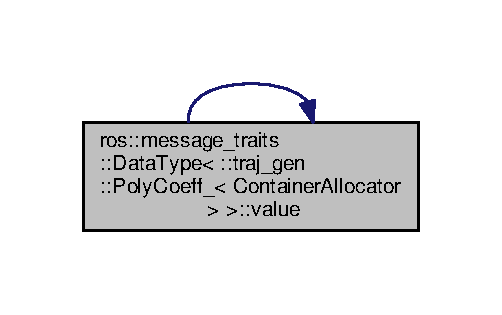
\includegraphics[width=241pt]{structros_1_1message__traits_1_1_data_type_3_01_1_1traj__gen_1_1_poly_coeff___3_01_container_allocator_01_4_01_4_a785e6d39c2c99e53bbb56485af512bec_cgraph}
\end{center}
\end{figure}




Here is the caller graph for this function\+:
\nopagebreak
\begin{figure}[H]
\begin{center}
\leavevmode
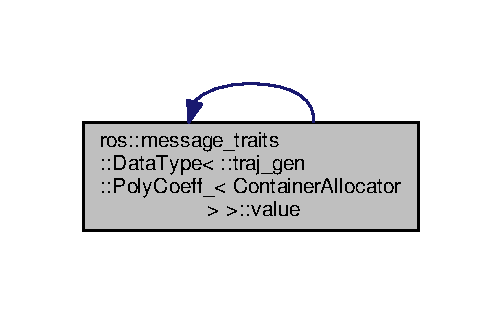
\includegraphics[width=241pt]{structros_1_1message__traits_1_1_data_type_3_01_1_1traj__gen_1_1_poly_coeff___3_01_container_allocator_01_4_01_4_a785e6d39c2c99e53bbb56485af512bec_icgraph}
\end{center}
\end{figure}




The documentation for this struct was generated from the following file\+:\begin{DoxyCompactItemize}
\item 
build/devel/include/traj\+\_\+gen/\hyperlink{_poly_coeff_8h}{Poly\+Coeff.\+h}\end{DoxyCompactItemize}

\hypertarget{structros_1_1message__traits_1_1_data_type_3_01_1_1traj__gen_1_1_poly_spline___3_01_container_allocator_01_4_01_4}{}\section{ros\+:\+:message\+\_\+traits\+:\+:Data\+Type$<$ \+:\+:traj\+\_\+gen\+:\+:Poly\+Spline\+\_\+$<$ Container\+Allocator $>$ $>$ Struct Template Reference}
\label{structros_1_1message__traits_1_1_data_type_3_01_1_1traj__gen_1_1_poly_spline___3_01_container_allocator_01_4_01_4}\index{ros\+::message\+\_\+traits\+::\+Data\+Type$<$ \+::traj\+\_\+gen\+::\+Poly\+Spline\+\_\+$<$ Container\+Allocator $>$ $>$@{ros\+::message\+\_\+traits\+::\+Data\+Type$<$ \+::traj\+\_\+gen\+::\+Poly\+Spline\+\_\+$<$ Container\+Allocator $>$ $>$}}


{\ttfamily \#include $<$Poly\+Spline.\+h$>$}

\subsection*{Static Public Member Functions}
\begin{DoxyCompactItemize}
\item 
static const char $\ast$ \hyperlink{structros_1_1message__traits_1_1_data_type_3_01_1_1traj__gen_1_1_poly_spline___3_01_container_allocator_01_4_01_4_abf220744a93c13e24c48a5ab57ef9fe6}{value} ()
\item 
static const char $\ast$ \hyperlink{structros_1_1message__traits_1_1_data_type_3_01_1_1traj__gen_1_1_poly_spline___3_01_container_allocator_01_4_01_4_a863abb98380ce9000983ca441a37a7b8}{value} (const \+::\hyperlink{structtraj__gen_1_1_poly_spline__}{traj\+\_\+gen\+::\+Poly\+Spline\+\_\+}$<$ Container\+Allocator $>$ \&)
\end{DoxyCompactItemize}


\subsection{Detailed Description}
\subsubsection*{template$<$class Container\+Allocator$>$\\*
struct ros\+::message\+\_\+traits\+::\+Data\+Type$<$ \+::traj\+\_\+gen\+::\+Poly\+Spline\+\_\+$<$ Container\+Allocator $>$ $>$}



Definition at line 142 of file Poly\+Spline.\+h.



\subsection{Member Function Documentation}
\index{ros\+::message\+\_\+traits\+::\+Data\+Type$<$ \+::traj\+\_\+gen\+::\+Poly\+Spline\+\_\+$<$ Container\+Allocator $>$ $>$@{ros\+::message\+\_\+traits\+::\+Data\+Type$<$ \+::traj\+\_\+gen\+::\+Poly\+Spline\+\_\+$<$ Container\+Allocator $>$ $>$}!value@{value}}
\index{value@{value}!ros\+::message\+\_\+traits\+::\+Data\+Type$<$ \+::traj\+\_\+gen\+::\+Poly\+Spline\+\_\+$<$ Container\+Allocator $>$ $>$@{ros\+::message\+\_\+traits\+::\+Data\+Type$<$ \+::traj\+\_\+gen\+::\+Poly\+Spline\+\_\+$<$ Container\+Allocator $>$ $>$}}
\subsubsection[{\texorpdfstring{value()}{value()}}]{\setlength{\rightskip}{0pt plus 5cm}template$<$class Container\+Allocator $>$ static const char$\ast$ ros\+::message\+\_\+traits\+::\+Data\+Type$<$ \+::{\bf traj\+\_\+gen\+::\+Poly\+Spline\+\_\+}$<$ Container\+Allocator $>$ $>$\+::value (
\begin{DoxyParamCaption}
{}
\end{DoxyParamCaption}
)\hspace{0.3cm}{\ttfamily [inline]}, {\ttfamily [static]}}\hypertarget{structros_1_1message__traits_1_1_data_type_3_01_1_1traj__gen_1_1_poly_spline___3_01_container_allocator_01_4_01_4_abf220744a93c13e24c48a5ab57ef9fe6}{}\label{structros_1_1message__traits_1_1_data_type_3_01_1_1traj__gen_1_1_poly_spline___3_01_container_allocator_01_4_01_4_abf220744a93c13e24c48a5ab57ef9fe6}


Definition at line 144 of file Poly\+Spline.\+h.

\index{ros\+::message\+\_\+traits\+::\+Data\+Type$<$ \+::traj\+\_\+gen\+::\+Poly\+Spline\+\_\+$<$ Container\+Allocator $>$ $>$@{ros\+::message\+\_\+traits\+::\+Data\+Type$<$ \+::traj\+\_\+gen\+::\+Poly\+Spline\+\_\+$<$ Container\+Allocator $>$ $>$}!value@{value}}
\index{value@{value}!ros\+::message\+\_\+traits\+::\+Data\+Type$<$ \+::traj\+\_\+gen\+::\+Poly\+Spline\+\_\+$<$ Container\+Allocator $>$ $>$@{ros\+::message\+\_\+traits\+::\+Data\+Type$<$ \+::traj\+\_\+gen\+::\+Poly\+Spline\+\_\+$<$ Container\+Allocator $>$ $>$}}
\subsubsection[{\texorpdfstring{value(const \+::traj\+\_\+gen\+::\+Poly\+Spline\+\_\+$<$ Container\+Allocator $>$ \&)}{value(const ::traj_gen::PolySpline_< ContainerAllocator > &)}}]{\setlength{\rightskip}{0pt plus 5cm}template$<$class Container\+Allocator $>$ static const char$\ast$ ros\+::message\+\_\+traits\+::\+Data\+Type$<$ \+::{\bf traj\+\_\+gen\+::\+Poly\+Spline\+\_\+}$<$ Container\+Allocator $>$ $>$\+::value (
\begin{DoxyParamCaption}
\item[{const \+::{\bf traj\+\_\+gen\+::\+Poly\+Spline\+\_\+}$<$ Container\+Allocator $>$ \&}]{}
\end{DoxyParamCaption}
)\hspace{0.3cm}{\ttfamily [inline]}, {\ttfamily [static]}}\hypertarget{structros_1_1message__traits_1_1_data_type_3_01_1_1traj__gen_1_1_poly_spline___3_01_container_allocator_01_4_01_4_a863abb98380ce9000983ca441a37a7b8}{}\label{structros_1_1message__traits_1_1_data_type_3_01_1_1traj__gen_1_1_poly_spline___3_01_container_allocator_01_4_01_4_a863abb98380ce9000983ca441a37a7b8}


Definition at line 149 of file Poly\+Spline.\+h.



Here is the call graph for this function\+:
\nopagebreak
\begin{figure}[H]
\begin{center}
\leavevmode
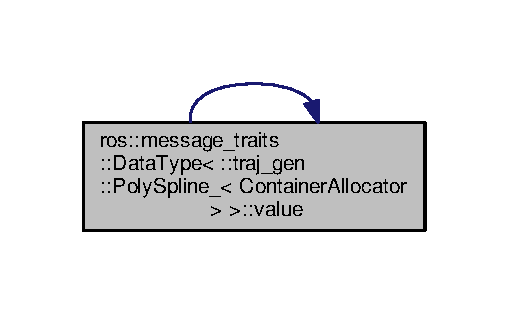
\includegraphics[width=244pt]{structros_1_1message__traits_1_1_data_type_3_01_1_1traj__gen_1_1_poly_spline___3_01_container_allocator_01_4_01_4_a863abb98380ce9000983ca441a37a7b8_cgraph}
\end{center}
\end{figure}




Here is the caller graph for this function\+:
\nopagebreak
\begin{figure}[H]
\begin{center}
\leavevmode
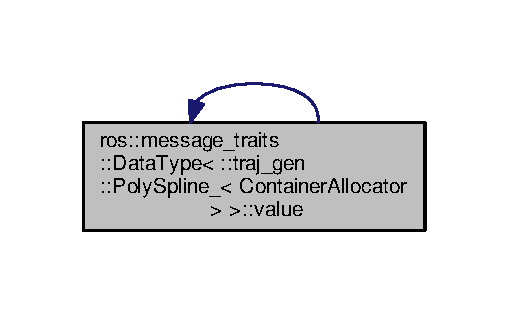
\includegraphics[width=244pt]{structros_1_1message__traits_1_1_data_type_3_01_1_1traj__gen_1_1_poly_spline___3_01_container_allocator_01_4_01_4_a863abb98380ce9000983ca441a37a7b8_icgraph}
\end{center}
\end{figure}




The documentation for this struct was generated from the following file\+:\begin{DoxyCompactItemize}
\item 
build/devel/include/traj\+\_\+gen/\hyperlink{_poly_spline_8h}{Poly\+Spline.\+h}\end{DoxyCompactItemize}

\hypertarget{structros_1_1message__traits_1_1_data_type_3_01_1_1traj__gen_1_1_poly_spline_x_y_z___3_01_container_allocator_01_4_01_4}{}\section{ros\+:\+:message\+\_\+traits\+:\+:Data\+Type$<$ \+:\+:traj\+\_\+gen\+:\+:Poly\+Spline\+X\+Y\+Z\+\_\+$<$ Container\+Allocator $>$ $>$ Struct Template Reference}
\label{structros_1_1message__traits_1_1_data_type_3_01_1_1traj__gen_1_1_poly_spline_x_y_z___3_01_container_allocator_01_4_01_4}\index{ros\+::message\+\_\+traits\+::\+Data\+Type$<$ \+::traj\+\_\+gen\+::\+Poly\+Spline\+X\+Y\+Z\+\_\+$<$ Container\+Allocator $>$ $>$@{ros\+::message\+\_\+traits\+::\+Data\+Type$<$ \+::traj\+\_\+gen\+::\+Poly\+Spline\+X\+Y\+Z\+\_\+$<$ Container\+Allocator $>$ $>$}}


{\ttfamily \#include $<$Poly\+Spline\+X\+Y\+Z.\+h$>$}

\subsection*{Static Public Member Functions}
\begin{DoxyCompactItemize}
\item 
static const char $\ast$ \hyperlink{structros_1_1message__traits_1_1_data_type_3_01_1_1traj__gen_1_1_poly_spline_x_y_z___3_01_container_allocator_01_4_01_4_aad7ae669852627b5d93b6db20f4734a0}{value} ()
\item 
static const char $\ast$ \hyperlink{structros_1_1message__traits_1_1_data_type_3_01_1_1traj__gen_1_1_poly_spline_x_y_z___3_01_container_allocator_01_4_01_4_aef66fdb342509b0f76cde06cca36fed6}{value} (const \+::\hyperlink{structtraj__gen_1_1_poly_spline_x_y_z__}{traj\+\_\+gen\+::\+Poly\+Spline\+X\+Y\+Z\+\_\+}$<$ Container\+Allocator $>$ \&)
\end{DoxyCompactItemize}


\subsection{Detailed Description}
\subsubsection*{template$<$class Container\+Allocator$>$\\*
struct ros\+::message\+\_\+traits\+::\+Data\+Type$<$ \+::traj\+\_\+gen\+::\+Poly\+Spline\+X\+Y\+Z\+\_\+$<$ Container\+Allocator $>$ $>$}



Definition at line 159 of file Poly\+Spline\+X\+Y\+Z.\+h.



\subsection{Member Function Documentation}
\index{ros\+::message\+\_\+traits\+::\+Data\+Type$<$ \+::traj\+\_\+gen\+::\+Poly\+Spline\+X\+Y\+Z\+\_\+$<$ Container\+Allocator $>$ $>$@{ros\+::message\+\_\+traits\+::\+Data\+Type$<$ \+::traj\+\_\+gen\+::\+Poly\+Spline\+X\+Y\+Z\+\_\+$<$ Container\+Allocator $>$ $>$}!value@{value}}
\index{value@{value}!ros\+::message\+\_\+traits\+::\+Data\+Type$<$ \+::traj\+\_\+gen\+::\+Poly\+Spline\+X\+Y\+Z\+\_\+$<$ Container\+Allocator $>$ $>$@{ros\+::message\+\_\+traits\+::\+Data\+Type$<$ \+::traj\+\_\+gen\+::\+Poly\+Spline\+X\+Y\+Z\+\_\+$<$ Container\+Allocator $>$ $>$}}
\subsubsection[{\texorpdfstring{value()}{value()}}]{\setlength{\rightskip}{0pt plus 5cm}template$<$class Container\+Allocator $>$ static const char$\ast$ ros\+::message\+\_\+traits\+::\+Data\+Type$<$ \+::{\bf traj\+\_\+gen\+::\+Poly\+Spline\+X\+Y\+Z\+\_\+}$<$ Container\+Allocator $>$ $>$\+::value (
\begin{DoxyParamCaption}
{}
\end{DoxyParamCaption}
)\hspace{0.3cm}{\ttfamily [inline]}, {\ttfamily [static]}}\hypertarget{structros_1_1message__traits_1_1_data_type_3_01_1_1traj__gen_1_1_poly_spline_x_y_z___3_01_container_allocator_01_4_01_4_aad7ae669852627b5d93b6db20f4734a0}{}\label{structros_1_1message__traits_1_1_data_type_3_01_1_1traj__gen_1_1_poly_spline_x_y_z___3_01_container_allocator_01_4_01_4_aad7ae669852627b5d93b6db20f4734a0}


Definition at line 161 of file Poly\+Spline\+X\+Y\+Z.\+h.

\index{ros\+::message\+\_\+traits\+::\+Data\+Type$<$ \+::traj\+\_\+gen\+::\+Poly\+Spline\+X\+Y\+Z\+\_\+$<$ Container\+Allocator $>$ $>$@{ros\+::message\+\_\+traits\+::\+Data\+Type$<$ \+::traj\+\_\+gen\+::\+Poly\+Spline\+X\+Y\+Z\+\_\+$<$ Container\+Allocator $>$ $>$}!value@{value}}
\index{value@{value}!ros\+::message\+\_\+traits\+::\+Data\+Type$<$ \+::traj\+\_\+gen\+::\+Poly\+Spline\+X\+Y\+Z\+\_\+$<$ Container\+Allocator $>$ $>$@{ros\+::message\+\_\+traits\+::\+Data\+Type$<$ \+::traj\+\_\+gen\+::\+Poly\+Spline\+X\+Y\+Z\+\_\+$<$ Container\+Allocator $>$ $>$}}
\subsubsection[{\texorpdfstring{value(const \+::traj\+\_\+gen\+::\+Poly\+Spline\+X\+Y\+Z\+\_\+$<$ Container\+Allocator $>$ \&)}{value(const ::traj_gen::PolySplineXYZ_< ContainerAllocator > &)}}]{\setlength{\rightskip}{0pt plus 5cm}template$<$class Container\+Allocator $>$ static const char$\ast$ ros\+::message\+\_\+traits\+::\+Data\+Type$<$ \+::{\bf traj\+\_\+gen\+::\+Poly\+Spline\+X\+Y\+Z\+\_\+}$<$ Container\+Allocator $>$ $>$\+::value (
\begin{DoxyParamCaption}
\item[{const \+::{\bf traj\+\_\+gen\+::\+Poly\+Spline\+X\+Y\+Z\+\_\+}$<$ Container\+Allocator $>$ \&}]{}
\end{DoxyParamCaption}
)\hspace{0.3cm}{\ttfamily [inline]}, {\ttfamily [static]}}\hypertarget{structros_1_1message__traits_1_1_data_type_3_01_1_1traj__gen_1_1_poly_spline_x_y_z___3_01_container_allocator_01_4_01_4_aef66fdb342509b0f76cde06cca36fed6}{}\label{structros_1_1message__traits_1_1_data_type_3_01_1_1traj__gen_1_1_poly_spline_x_y_z___3_01_container_allocator_01_4_01_4_aef66fdb342509b0f76cde06cca36fed6}


Definition at line 166 of file Poly\+Spline\+X\+Y\+Z.\+h.



Here is the call graph for this function\+:
\nopagebreak
\begin{figure}[H]
\begin{center}
\leavevmode
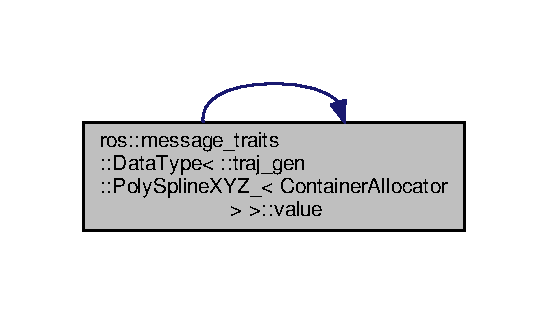
\includegraphics[width=263pt]{structros_1_1message__traits_1_1_data_type_3_01_1_1traj__gen_1_1_poly_spline_x_y_z___3_01_container_allocator_01_4_01_4_aef66fdb342509b0f76cde06cca36fed6_cgraph}
\end{center}
\end{figure}




Here is the caller graph for this function\+:
\nopagebreak
\begin{figure}[H]
\begin{center}
\leavevmode
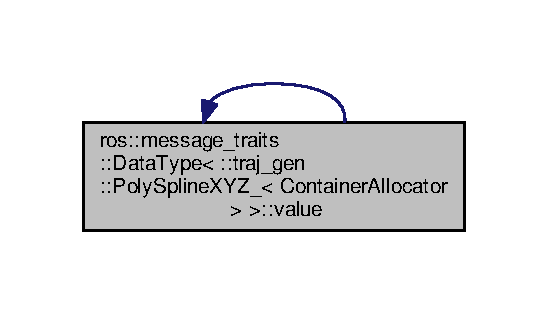
\includegraphics[width=263pt]{structros_1_1message__traits_1_1_data_type_3_01_1_1traj__gen_1_1_poly_spline_x_y_z___3_01_container_allocator_01_4_01_4_aef66fdb342509b0f76cde06cca36fed6_icgraph}
\end{center}
\end{figure}




The documentation for this struct was generated from the following file\+:\begin{DoxyCompactItemize}
\item 
build/devel/include/traj\+\_\+gen/\hyperlink{_poly_spline_x_y_z_8h}{Poly\+Spline\+X\+Y\+Z.\+h}\end{DoxyCompactItemize}

\hypertarget{structros_1_1service__traits_1_1_data_type_3_01_1_1traj__gen_1_1_spline_gen_01_4}{}\section{ros\+:\+:service\+\_\+traits\+:\+:Data\+Type$<$ \+:\+:traj\+\_\+gen\+:\+:Spline\+Gen $>$ Struct Template Reference}
\label{structros_1_1service__traits_1_1_data_type_3_01_1_1traj__gen_1_1_spline_gen_01_4}\index{ros\+::service\+\_\+traits\+::\+Data\+Type$<$ \+::traj\+\_\+gen\+::\+Spline\+Gen $>$@{ros\+::service\+\_\+traits\+::\+Data\+Type$<$ \+::traj\+\_\+gen\+::\+Spline\+Gen $>$}}


{\ttfamily \#include $<$Spline\+Gen.\+h$>$}

\subsection*{Static Public Member Functions}
\begin{DoxyCompactItemize}
\item 
static const char $\ast$ \hyperlink{structros_1_1service__traits_1_1_data_type_3_01_1_1traj__gen_1_1_spline_gen_01_4_aa360a20278d15909d7e95f8d4c7b2f00}{value} ()
\item 
static const char $\ast$ \hyperlink{structros_1_1service__traits_1_1_data_type_3_01_1_1traj__gen_1_1_spline_gen_01_4_aa91f4492b3cdee93fc56964c34c38101}{value} (const \+::\hyperlink{structtraj__gen_1_1_spline_gen}{traj\+\_\+gen\+::\+Spline\+Gen} \&)
\end{DoxyCompactItemize}


\subsection{Detailed Description}
\subsubsection*{template$<$$>$\\*
struct ros\+::service\+\_\+traits\+::\+Data\+Type$<$ \+::traj\+\_\+gen\+::\+Spline\+Gen $>$}



Definition at line 50 of file Spline\+Gen.\+h.



\subsection{Member Function Documentation}
\index{ros\+::service\+\_\+traits\+::\+Data\+Type$<$ \+::traj\+\_\+gen\+::\+Spline\+Gen $>$@{ros\+::service\+\_\+traits\+::\+Data\+Type$<$ \+::traj\+\_\+gen\+::\+Spline\+Gen $>$}!value@{value}}
\index{value@{value}!ros\+::service\+\_\+traits\+::\+Data\+Type$<$ \+::traj\+\_\+gen\+::\+Spline\+Gen $>$@{ros\+::service\+\_\+traits\+::\+Data\+Type$<$ \+::traj\+\_\+gen\+::\+Spline\+Gen $>$}}
\subsubsection[{\texorpdfstring{value()}{value()}}]{\setlength{\rightskip}{0pt plus 5cm}static const char$\ast$ ros\+::service\+\_\+traits\+::\+Data\+Type$<$ \+::{\bf traj\+\_\+gen\+::\+Spline\+Gen} $>$\+::value (
\begin{DoxyParamCaption}
{}
\end{DoxyParamCaption}
)\hspace{0.3cm}{\ttfamily [inline]}, {\ttfamily [static]}}\hypertarget{structros_1_1service__traits_1_1_data_type_3_01_1_1traj__gen_1_1_spline_gen_01_4_aa360a20278d15909d7e95f8d4c7b2f00}{}\label{structros_1_1service__traits_1_1_data_type_3_01_1_1traj__gen_1_1_spline_gen_01_4_aa360a20278d15909d7e95f8d4c7b2f00}


Definition at line 51 of file Spline\+Gen.\+h.

\index{ros\+::service\+\_\+traits\+::\+Data\+Type$<$ \+::traj\+\_\+gen\+::\+Spline\+Gen $>$@{ros\+::service\+\_\+traits\+::\+Data\+Type$<$ \+::traj\+\_\+gen\+::\+Spline\+Gen $>$}!value@{value}}
\index{value@{value}!ros\+::service\+\_\+traits\+::\+Data\+Type$<$ \+::traj\+\_\+gen\+::\+Spline\+Gen $>$@{ros\+::service\+\_\+traits\+::\+Data\+Type$<$ \+::traj\+\_\+gen\+::\+Spline\+Gen $>$}}
\subsubsection[{\texorpdfstring{value(const \+::traj\+\_\+gen\+::\+Spline\+Gen \&)}{value(const ::traj_gen::SplineGen &)}}]{\setlength{\rightskip}{0pt plus 5cm}static const char$\ast$ ros\+::service\+\_\+traits\+::\+Data\+Type$<$ \+::{\bf traj\+\_\+gen\+::\+Spline\+Gen} $>$\+::value (
\begin{DoxyParamCaption}
\item[{const \+::{\bf traj\+\_\+gen\+::\+Spline\+Gen} \&}]{}
\end{DoxyParamCaption}
)\hspace{0.3cm}{\ttfamily [inline]}, {\ttfamily [static]}}\hypertarget{structros_1_1service__traits_1_1_data_type_3_01_1_1traj__gen_1_1_spline_gen_01_4_aa91f4492b3cdee93fc56964c34c38101}{}\label{structros_1_1service__traits_1_1_data_type_3_01_1_1traj__gen_1_1_spline_gen_01_4_aa91f4492b3cdee93fc56964c34c38101}


Definition at line 56 of file Spline\+Gen.\+h.



Here is the call graph for this function\+:
\nopagebreak
\begin{figure}[H]
\begin{center}
\leavevmode
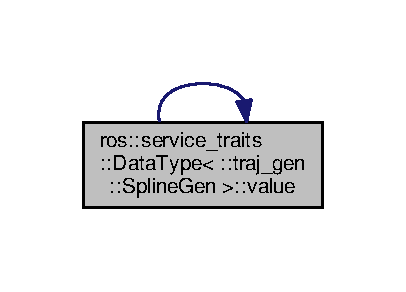
\includegraphics[width=195pt]{structros_1_1service__traits_1_1_data_type_3_01_1_1traj__gen_1_1_spline_gen_01_4_aa91f4492b3cdee93fc56964c34c38101_cgraph}
\end{center}
\end{figure}




Here is the caller graph for this function\+:
\nopagebreak
\begin{figure}[H]
\begin{center}
\leavevmode
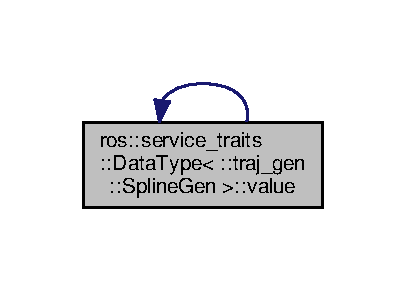
\includegraphics[width=195pt]{structros_1_1service__traits_1_1_data_type_3_01_1_1traj__gen_1_1_spline_gen_01_4_aa91f4492b3cdee93fc56964c34c38101_icgraph}
\end{center}
\end{figure}




The documentation for this struct was generated from the following file\+:\begin{DoxyCompactItemize}
\item 
build/devel/include/traj\+\_\+gen/\hyperlink{_spline_gen_8h}{Spline\+Gen.\+h}\end{DoxyCompactItemize}

\hypertarget{structros_1_1service__traits_1_1_data_type_3_01_1_1traj__gen_1_1_spline_gen_request_01_4}{}\section{ros\+:\+:service\+\_\+traits\+:\+:Data\+Type$<$ \+:\+:traj\+\_\+gen\+:\+:Spline\+Gen\+Request $>$ Struct Template Reference}
\label{structros_1_1service__traits_1_1_data_type_3_01_1_1traj__gen_1_1_spline_gen_request_01_4}\index{ros\+::service\+\_\+traits\+::\+Data\+Type$<$ \+::traj\+\_\+gen\+::\+Spline\+Gen\+Request $>$@{ros\+::service\+\_\+traits\+::\+Data\+Type$<$ \+::traj\+\_\+gen\+::\+Spline\+Gen\+Request $>$}}


{\ttfamily \#include $<$Spline\+Gen.\+h$>$}

\subsection*{Static Public Member Functions}
\begin{DoxyCompactItemize}
\item 
static const char $\ast$ \hyperlink{structros_1_1service__traits_1_1_data_type_3_01_1_1traj__gen_1_1_spline_gen_request_01_4_ad03f668be543ebe2bcbf86fcdf5e9ada}{value} ()
\item 
static const char $\ast$ \hyperlink{structros_1_1service__traits_1_1_data_type_3_01_1_1traj__gen_1_1_spline_gen_request_01_4_a3c13cdfe6379ae122c7189f0faff78b6}{value} (const \+::\hyperlink{namespacetraj__gen_a61c65203f503c18d4b3cb68b9ee74a74}{traj\+\_\+gen\+::\+Spline\+Gen\+Request} \&)
\end{DoxyCompactItemize}


\subsection{Detailed Description}
\subsubsection*{template$<$$>$\\*
struct ros\+::service\+\_\+traits\+::\+Data\+Type$<$ \+::traj\+\_\+gen\+::\+Spline\+Gen\+Request $>$}



Definition at line 78 of file Spline\+Gen.\+h.



\subsection{Member Function Documentation}
\index{ros\+::service\+\_\+traits\+::\+Data\+Type$<$ \+::traj\+\_\+gen\+::\+Spline\+Gen\+Request $>$@{ros\+::service\+\_\+traits\+::\+Data\+Type$<$ \+::traj\+\_\+gen\+::\+Spline\+Gen\+Request $>$}!value@{value}}
\index{value@{value}!ros\+::service\+\_\+traits\+::\+Data\+Type$<$ \+::traj\+\_\+gen\+::\+Spline\+Gen\+Request $>$@{ros\+::service\+\_\+traits\+::\+Data\+Type$<$ \+::traj\+\_\+gen\+::\+Spline\+Gen\+Request $>$}}
\subsubsection[{\texorpdfstring{value()}{value()}}]{\setlength{\rightskip}{0pt plus 5cm}static const char$\ast$ ros\+::service\+\_\+traits\+::\+Data\+Type$<$ \+::{\bf traj\+\_\+gen\+::\+Spline\+Gen\+Request} $>$\+::value (
\begin{DoxyParamCaption}
{}
\end{DoxyParamCaption}
)\hspace{0.3cm}{\ttfamily [inline]}, {\ttfamily [static]}}\hypertarget{structros_1_1service__traits_1_1_data_type_3_01_1_1traj__gen_1_1_spline_gen_request_01_4_ad03f668be543ebe2bcbf86fcdf5e9ada}{}\label{structros_1_1service__traits_1_1_data_type_3_01_1_1traj__gen_1_1_spline_gen_request_01_4_ad03f668be543ebe2bcbf86fcdf5e9ada}


Definition at line 80 of file Spline\+Gen.\+h.

\index{ros\+::service\+\_\+traits\+::\+Data\+Type$<$ \+::traj\+\_\+gen\+::\+Spline\+Gen\+Request $>$@{ros\+::service\+\_\+traits\+::\+Data\+Type$<$ \+::traj\+\_\+gen\+::\+Spline\+Gen\+Request $>$}!value@{value}}
\index{value@{value}!ros\+::service\+\_\+traits\+::\+Data\+Type$<$ \+::traj\+\_\+gen\+::\+Spline\+Gen\+Request $>$@{ros\+::service\+\_\+traits\+::\+Data\+Type$<$ \+::traj\+\_\+gen\+::\+Spline\+Gen\+Request $>$}}
\subsubsection[{\texorpdfstring{value(const \+::traj\+\_\+gen\+::\+Spline\+Gen\+Request \&)}{value(const ::traj_gen::SplineGenRequest &)}}]{\setlength{\rightskip}{0pt plus 5cm}static const char$\ast$ ros\+::service\+\_\+traits\+::\+Data\+Type$<$ \+::{\bf traj\+\_\+gen\+::\+Spline\+Gen\+Request} $>$\+::value (
\begin{DoxyParamCaption}
\item[{const \+::{\bf traj\+\_\+gen\+::\+Spline\+Gen\+Request} \&}]{}
\end{DoxyParamCaption}
)\hspace{0.3cm}{\ttfamily [inline]}, {\ttfamily [static]}}\hypertarget{structros_1_1service__traits_1_1_data_type_3_01_1_1traj__gen_1_1_spline_gen_request_01_4_a3c13cdfe6379ae122c7189f0faff78b6}{}\label{structros_1_1service__traits_1_1_data_type_3_01_1_1traj__gen_1_1_spline_gen_request_01_4_a3c13cdfe6379ae122c7189f0faff78b6}


Definition at line 84 of file Spline\+Gen.\+h.



The documentation for this struct was generated from the following file\+:\begin{DoxyCompactItemize}
\item 
build/devel/include/traj\+\_\+gen/\hyperlink{_spline_gen_8h}{Spline\+Gen.\+h}\end{DoxyCompactItemize}

\hypertarget{structros_1_1message__traits_1_1_data_type_3_01_1_1traj__gen_1_1_spline_gen_request___3_01_container_allocator_01_4_01_4}{}\section{ros\+:\+:message\+\_\+traits\+:\+:Data\+Type$<$ \+:\+:traj\+\_\+gen\+:\+:Spline\+Gen\+Request\+\_\+$<$ Container\+Allocator $>$ $>$ Struct Template Reference}
\label{structros_1_1message__traits_1_1_data_type_3_01_1_1traj__gen_1_1_spline_gen_request___3_01_container_allocator_01_4_01_4}\index{ros\+::message\+\_\+traits\+::\+Data\+Type$<$ \+::traj\+\_\+gen\+::\+Spline\+Gen\+Request\+\_\+$<$ Container\+Allocator $>$ $>$@{ros\+::message\+\_\+traits\+::\+Data\+Type$<$ \+::traj\+\_\+gen\+::\+Spline\+Gen\+Request\+\_\+$<$ Container\+Allocator $>$ $>$}}


{\ttfamily \#include $<$Spline\+Gen\+Request.\+h$>$}

\subsection*{Static Public Member Functions}
\begin{DoxyCompactItemize}
\item 
static const char $\ast$ \hyperlink{structros_1_1message__traits_1_1_data_type_3_01_1_1traj__gen_1_1_spline_gen_request___3_01_container_allocator_01_4_01_4_ad95d6fa2549039e7036babe5957141d0}{value} ()
\item 
static const char $\ast$ \hyperlink{structros_1_1message__traits_1_1_data_type_3_01_1_1traj__gen_1_1_spline_gen_request___3_01_container_allocator_01_4_01_4_a6b0da019adeec8ef9f47f6297c4d8031}{value} (const \+::\hyperlink{structtraj__gen_1_1_spline_gen_request__}{traj\+\_\+gen\+::\+Spline\+Gen\+Request\+\_\+}$<$ Container\+Allocator $>$ \&)
\end{DoxyCompactItemize}


\subsection{Detailed Description}
\subsubsection*{template$<$class Container\+Allocator$>$\\*
struct ros\+::message\+\_\+traits\+::\+Data\+Type$<$ \+::traj\+\_\+gen\+::\+Spline\+Gen\+Request\+\_\+$<$ Container\+Allocator $>$ $>$}



Definition at line 138 of file Spline\+Gen\+Request.\+h.



\subsection{Member Function Documentation}
\index{ros\+::message\+\_\+traits\+::\+Data\+Type$<$ \+::traj\+\_\+gen\+::\+Spline\+Gen\+Request\+\_\+$<$ Container\+Allocator $>$ $>$@{ros\+::message\+\_\+traits\+::\+Data\+Type$<$ \+::traj\+\_\+gen\+::\+Spline\+Gen\+Request\+\_\+$<$ Container\+Allocator $>$ $>$}!value@{value}}
\index{value@{value}!ros\+::message\+\_\+traits\+::\+Data\+Type$<$ \+::traj\+\_\+gen\+::\+Spline\+Gen\+Request\+\_\+$<$ Container\+Allocator $>$ $>$@{ros\+::message\+\_\+traits\+::\+Data\+Type$<$ \+::traj\+\_\+gen\+::\+Spline\+Gen\+Request\+\_\+$<$ Container\+Allocator $>$ $>$}}
\subsubsection[{\texorpdfstring{value()}{value()}}]{\setlength{\rightskip}{0pt plus 5cm}template$<$class Container\+Allocator $>$ static const char$\ast$ ros\+::message\+\_\+traits\+::\+Data\+Type$<$ \+::{\bf traj\+\_\+gen\+::\+Spline\+Gen\+Request\+\_\+}$<$ Container\+Allocator $>$ $>$\+::value (
\begin{DoxyParamCaption}
{}
\end{DoxyParamCaption}
)\hspace{0.3cm}{\ttfamily [inline]}, {\ttfamily [static]}}\hypertarget{structros_1_1message__traits_1_1_data_type_3_01_1_1traj__gen_1_1_spline_gen_request___3_01_container_allocator_01_4_01_4_ad95d6fa2549039e7036babe5957141d0}{}\label{structros_1_1message__traits_1_1_data_type_3_01_1_1traj__gen_1_1_spline_gen_request___3_01_container_allocator_01_4_01_4_ad95d6fa2549039e7036babe5957141d0}


Definition at line 140 of file Spline\+Gen\+Request.\+h.

\index{ros\+::message\+\_\+traits\+::\+Data\+Type$<$ \+::traj\+\_\+gen\+::\+Spline\+Gen\+Request\+\_\+$<$ Container\+Allocator $>$ $>$@{ros\+::message\+\_\+traits\+::\+Data\+Type$<$ \+::traj\+\_\+gen\+::\+Spline\+Gen\+Request\+\_\+$<$ Container\+Allocator $>$ $>$}!value@{value}}
\index{value@{value}!ros\+::message\+\_\+traits\+::\+Data\+Type$<$ \+::traj\+\_\+gen\+::\+Spline\+Gen\+Request\+\_\+$<$ Container\+Allocator $>$ $>$@{ros\+::message\+\_\+traits\+::\+Data\+Type$<$ \+::traj\+\_\+gen\+::\+Spline\+Gen\+Request\+\_\+$<$ Container\+Allocator $>$ $>$}}
\subsubsection[{\texorpdfstring{value(const \+::traj\+\_\+gen\+::\+Spline\+Gen\+Request\+\_\+$<$ Container\+Allocator $>$ \&)}{value(const ::traj_gen::SplineGenRequest_< ContainerAllocator > &)}}]{\setlength{\rightskip}{0pt plus 5cm}template$<$class Container\+Allocator $>$ static const char$\ast$ ros\+::message\+\_\+traits\+::\+Data\+Type$<$ \+::{\bf traj\+\_\+gen\+::\+Spline\+Gen\+Request\+\_\+}$<$ Container\+Allocator $>$ $>$\+::value (
\begin{DoxyParamCaption}
\item[{const \+::{\bf traj\+\_\+gen\+::\+Spline\+Gen\+Request\+\_\+}$<$ Container\+Allocator $>$ \&}]{}
\end{DoxyParamCaption}
)\hspace{0.3cm}{\ttfamily [inline]}, {\ttfamily [static]}}\hypertarget{structros_1_1message__traits_1_1_data_type_3_01_1_1traj__gen_1_1_spline_gen_request___3_01_container_allocator_01_4_01_4_a6b0da019adeec8ef9f47f6297c4d8031}{}\label{structros_1_1message__traits_1_1_data_type_3_01_1_1traj__gen_1_1_spline_gen_request___3_01_container_allocator_01_4_01_4_a6b0da019adeec8ef9f47f6297c4d8031}


Definition at line 145 of file Spline\+Gen\+Request.\+h.



Here is the call graph for this function\+:
\nopagebreak
\begin{figure}[H]
\begin{center}
\leavevmode
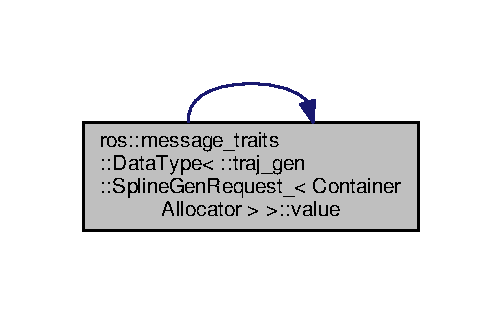
\includegraphics[width=241pt]{structros_1_1message__traits_1_1_data_type_3_01_1_1traj__gen_1_1_spline_gen_request___3_01_container_allocator_01_4_01_4_a6b0da019adeec8ef9f47f6297c4d8031_cgraph}
\end{center}
\end{figure}




Here is the caller graph for this function\+:
\nopagebreak
\begin{figure}[H]
\begin{center}
\leavevmode
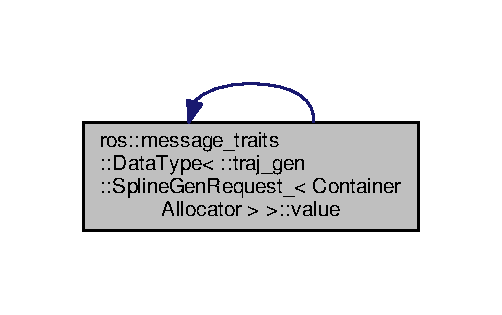
\includegraphics[width=241pt]{structros_1_1message__traits_1_1_data_type_3_01_1_1traj__gen_1_1_spline_gen_request___3_01_container_allocator_01_4_01_4_a6b0da019adeec8ef9f47f6297c4d8031_icgraph}
\end{center}
\end{figure}




The documentation for this struct was generated from the following file\+:\begin{DoxyCompactItemize}
\item 
build/devel/include/traj\+\_\+gen/\hyperlink{_spline_gen_request_8h}{Spline\+Gen\+Request.\+h}\end{DoxyCompactItemize}

\hypertarget{structros_1_1service__traits_1_1_data_type_3_01_1_1traj__gen_1_1_spline_gen_response_01_4}{}\section{ros\+:\+:service\+\_\+traits\+:\+:Data\+Type$<$ \+:\+:traj\+\_\+gen\+:\+:Spline\+Gen\+Response $>$ Struct Template Reference}
\label{structros_1_1service__traits_1_1_data_type_3_01_1_1traj__gen_1_1_spline_gen_response_01_4}\index{ros\+::service\+\_\+traits\+::\+Data\+Type$<$ \+::traj\+\_\+gen\+::\+Spline\+Gen\+Response $>$@{ros\+::service\+\_\+traits\+::\+Data\+Type$<$ \+::traj\+\_\+gen\+::\+Spline\+Gen\+Response $>$}}


{\ttfamily \#include $<$Spline\+Gen.\+h$>$}

\subsection*{Static Public Member Functions}
\begin{DoxyCompactItemize}
\item 
static const char $\ast$ \hyperlink{structros_1_1service__traits_1_1_data_type_3_01_1_1traj__gen_1_1_spline_gen_response_01_4_a0c3631365939cd0761d86402eafb750a}{value} ()
\item 
static const char $\ast$ \hyperlink{structros_1_1service__traits_1_1_data_type_3_01_1_1traj__gen_1_1_spline_gen_response_01_4_a4e1706302b9bc17743ddd940a66a393c}{value} (const \+::\hyperlink{namespacetraj__gen_a96b15a7eb1a4a1209fba2e9d75acb7a4}{traj\+\_\+gen\+::\+Spline\+Gen\+Response} \&)
\end{DoxyCompactItemize}


\subsection{Detailed Description}
\subsubsection*{template$<$$>$\\*
struct ros\+::service\+\_\+traits\+::\+Data\+Type$<$ \+::traj\+\_\+gen\+::\+Spline\+Gen\+Response $>$}



Definition at line 108 of file Spline\+Gen.\+h.



\subsection{Member Function Documentation}
\index{ros\+::service\+\_\+traits\+::\+Data\+Type$<$ \+::traj\+\_\+gen\+::\+Spline\+Gen\+Response $>$@{ros\+::service\+\_\+traits\+::\+Data\+Type$<$ \+::traj\+\_\+gen\+::\+Spline\+Gen\+Response $>$}!value@{value}}
\index{value@{value}!ros\+::service\+\_\+traits\+::\+Data\+Type$<$ \+::traj\+\_\+gen\+::\+Spline\+Gen\+Response $>$@{ros\+::service\+\_\+traits\+::\+Data\+Type$<$ \+::traj\+\_\+gen\+::\+Spline\+Gen\+Response $>$}}
\subsubsection[{\texorpdfstring{value()}{value()}}]{\setlength{\rightskip}{0pt plus 5cm}static const char$\ast$ ros\+::service\+\_\+traits\+::\+Data\+Type$<$ \+::{\bf traj\+\_\+gen\+::\+Spline\+Gen\+Response} $>$\+::value (
\begin{DoxyParamCaption}
{}
\end{DoxyParamCaption}
)\hspace{0.3cm}{\ttfamily [inline]}, {\ttfamily [static]}}\hypertarget{structros_1_1service__traits_1_1_data_type_3_01_1_1traj__gen_1_1_spline_gen_response_01_4_a0c3631365939cd0761d86402eafb750a}{}\label{structros_1_1service__traits_1_1_data_type_3_01_1_1traj__gen_1_1_spline_gen_response_01_4_a0c3631365939cd0761d86402eafb750a}


Definition at line 110 of file Spline\+Gen.\+h.

\index{ros\+::service\+\_\+traits\+::\+Data\+Type$<$ \+::traj\+\_\+gen\+::\+Spline\+Gen\+Response $>$@{ros\+::service\+\_\+traits\+::\+Data\+Type$<$ \+::traj\+\_\+gen\+::\+Spline\+Gen\+Response $>$}!value@{value}}
\index{value@{value}!ros\+::service\+\_\+traits\+::\+Data\+Type$<$ \+::traj\+\_\+gen\+::\+Spline\+Gen\+Response $>$@{ros\+::service\+\_\+traits\+::\+Data\+Type$<$ \+::traj\+\_\+gen\+::\+Spline\+Gen\+Response $>$}}
\subsubsection[{\texorpdfstring{value(const \+::traj\+\_\+gen\+::\+Spline\+Gen\+Response \&)}{value(const ::traj_gen::SplineGenResponse &)}}]{\setlength{\rightskip}{0pt plus 5cm}static const char$\ast$ ros\+::service\+\_\+traits\+::\+Data\+Type$<$ \+::{\bf traj\+\_\+gen\+::\+Spline\+Gen\+Response} $>$\+::value (
\begin{DoxyParamCaption}
\item[{const \+::{\bf traj\+\_\+gen\+::\+Spline\+Gen\+Response} \&}]{}
\end{DoxyParamCaption}
)\hspace{0.3cm}{\ttfamily [inline]}, {\ttfamily [static]}}\hypertarget{structros_1_1service__traits_1_1_data_type_3_01_1_1traj__gen_1_1_spline_gen_response_01_4_a4e1706302b9bc17743ddd940a66a393c}{}\label{structros_1_1service__traits_1_1_data_type_3_01_1_1traj__gen_1_1_spline_gen_response_01_4_a4e1706302b9bc17743ddd940a66a393c}


Definition at line 114 of file Spline\+Gen.\+h.



The documentation for this struct was generated from the following file\+:\begin{DoxyCompactItemize}
\item 
build/devel/include/traj\+\_\+gen/\hyperlink{_spline_gen_8h}{Spline\+Gen.\+h}\end{DoxyCompactItemize}

\hypertarget{structros_1_1message__traits_1_1_data_type_3_01_1_1traj__gen_1_1_spline_gen_response___3_01_container_allocator_01_4_01_4}{}\section{ros\+:\+:message\+\_\+traits\+:\+:Data\+Type$<$ \+:\+:traj\+\_\+gen\+:\+:Spline\+Gen\+Response\+\_\+$<$ Container\+Allocator $>$ $>$ Struct Template Reference}
\label{structros_1_1message__traits_1_1_data_type_3_01_1_1traj__gen_1_1_spline_gen_response___3_01_container_allocator_01_4_01_4}\index{ros\+::message\+\_\+traits\+::\+Data\+Type$<$ \+::traj\+\_\+gen\+::\+Spline\+Gen\+Response\+\_\+$<$ Container\+Allocator $>$ $>$@{ros\+::message\+\_\+traits\+::\+Data\+Type$<$ \+::traj\+\_\+gen\+::\+Spline\+Gen\+Response\+\_\+$<$ Container\+Allocator $>$ $>$}}


{\ttfamily \#include $<$Spline\+Gen\+Response.\+h$>$}

\subsection*{Static Public Member Functions}
\begin{DoxyCompactItemize}
\item 
static const char $\ast$ \hyperlink{structros_1_1message__traits_1_1_data_type_3_01_1_1traj__gen_1_1_spline_gen_response___3_01_container_allocator_01_4_01_4_af738ed3697fc5c3607f5777166502bbf}{value} ()
\item 
static const char $\ast$ \hyperlink{structros_1_1message__traits_1_1_data_type_3_01_1_1traj__gen_1_1_spline_gen_response___3_01_container_allocator_01_4_01_4_a45333b91e9108b4ab9094322fcc1243b}{value} (const \+::\hyperlink{structtraj__gen_1_1_spline_gen_response__}{traj\+\_\+gen\+::\+Spline\+Gen\+Response\+\_\+}$<$ Container\+Allocator $>$ \&)
\end{DoxyCompactItemize}


\subsection{Detailed Description}
\subsubsection*{template$<$class Container\+Allocator$>$\\*
struct ros\+::message\+\_\+traits\+::\+Data\+Type$<$ \+::traj\+\_\+gen\+::\+Spline\+Gen\+Response\+\_\+$<$ Container\+Allocator $>$ $>$}



Definition at line 127 of file Spline\+Gen\+Response.\+h.



\subsection{Member Function Documentation}
\index{ros\+::message\+\_\+traits\+::\+Data\+Type$<$ \+::traj\+\_\+gen\+::\+Spline\+Gen\+Response\+\_\+$<$ Container\+Allocator $>$ $>$@{ros\+::message\+\_\+traits\+::\+Data\+Type$<$ \+::traj\+\_\+gen\+::\+Spline\+Gen\+Response\+\_\+$<$ Container\+Allocator $>$ $>$}!value@{value}}
\index{value@{value}!ros\+::message\+\_\+traits\+::\+Data\+Type$<$ \+::traj\+\_\+gen\+::\+Spline\+Gen\+Response\+\_\+$<$ Container\+Allocator $>$ $>$@{ros\+::message\+\_\+traits\+::\+Data\+Type$<$ \+::traj\+\_\+gen\+::\+Spline\+Gen\+Response\+\_\+$<$ Container\+Allocator $>$ $>$}}
\subsubsection[{\texorpdfstring{value()}{value()}}]{\setlength{\rightskip}{0pt plus 5cm}template$<$class Container\+Allocator $>$ static const char$\ast$ ros\+::message\+\_\+traits\+::\+Data\+Type$<$ \+::{\bf traj\+\_\+gen\+::\+Spline\+Gen\+Response\+\_\+}$<$ Container\+Allocator $>$ $>$\+::value (
\begin{DoxyParamCaption}
{}
\end{DoxyParamCaption}
)\hspace{0.3cm}{\ttfamily [inline]}, {\ttfamily [static]}}\hypertarget{structros_1_1message__traits_1_1_data_type_3_01_1_1traj__gen_1_1_spline_gen_response___3_01_container_allocator_01_4_01_4_af738ed3697fc5c3607f5777166502bbf}{}\label{structros_1_1message__traits_1_1_data_type_3_01_1_1traj__gen_1_1_spline_gen_response___3_01_container_allocator_01_4_01_4_af738ed3697fc5c3607f5777166502bbf}


Definition at line 129 of file Spline\+Gen\+Response.\+h.

\index{ros\+::message\+\_\+traits\+::\+Data\+Type$<$ \+::traj\+\_\+gen\+::\+Spline\+Gen\+Response\+\_\+$<$ Container\+Allocator $>$ $>$@{ros\+::message\+\_\+traits\+::\+Data\+Type$<$ \+::traj\+\_\+gen\+::\+Spline\+Gen\+Response\+\_\+$<$ Container\+Allocator $>$ $>$}!value@{value}}
\index{value@{value}!ros\+::message\+\_\+traits\+::\+Data\+Type$<$ \+::traj\+\_\+gen\+::\+Spline\+Gen\+Response\+\_\+$<$ Container\+Allocator $>$ $>$@{ros\+::message\+\_\+traits\+::\+Data\+Type$<$ \+::traj\+\_\+gen\+::\+Spline\+Gen\+Response\+\_\+$<$ Container\+Allocator $>$ $>$}}
\subsubsection[{\texorpdfstring{value(const \+::traj\+\_\+gen\+::\+Spline\+Gen\+Response\+\_\+$<$ Container\+Allocator $>$ \&)}{value(const ::traj_gen::SplineGenResponse_< ContainerAllocator > &)}}]{\setlength{\rightskip}{0pt plus 5cm}template$<$class Container\+Allocator $>$ static const char$\ast$ ros\+::message\+\_\+traits\+::\+Data\+Type$<$ \+::{\bf traj\+\_\+gen\+::\+Spline\+Gen\+Response\+\_\+}$<$ Container\+Allocator $>$ $>$\+::value (
\begin{DoxyParamCaption}
\item[{const \+::{\bf traj\+\_\+gen\+::\+Spline\+Gen\+Response\+\_\+}$<$ Container\+Allocator $>$ \&}]{}
\end{DoxyParamCaption}
)\hspace{0.3cm}{\ttfamily [inline]}, {\ttfamily [static]}}\hypertarget{structros_1_1message__traits_1_1_data_type_3_01_1_1traj__gen_1_1_spline_gen_response___3_01_container_allocator_01_4_01_4_a45333b91e9108b4ab9094322fcc1243b}{}\label{structros_1_1message__traits_1_1_data_type_3_01_1_1traj__gen_1_1_spline_gen_response___3_01_container_allocator_01_4_01_4_a45333b91e9108b4ab9094322fcc1243b}


Definition at line 134 of file Spline\+Gen\+Response.\+h.



Here is the call graph for this function\+:
\nopagebreak
\begin{figure}[H]
\begin{center}
\leavevmode
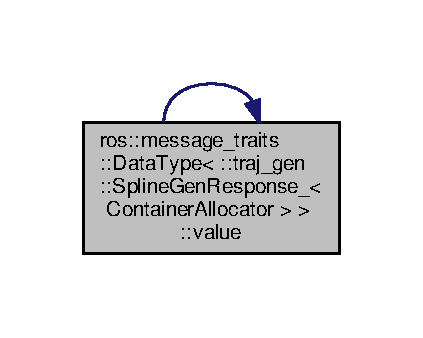
\includegraphics[width=203pt]{structros_1_1message__traits_1_1_data_type_3_01_1_1traj__gen_1_1_spline_gen_response___3_01_container_allocator_01_4_01_4_a45333b91e9108b4ab9094322fcc1243b_cgraph}
\end{center}
\end{figure}




Here is the caller graph for this function\+:
\nopagebreak
\begin{figure}[H]
\begin{center}
\leavevmode
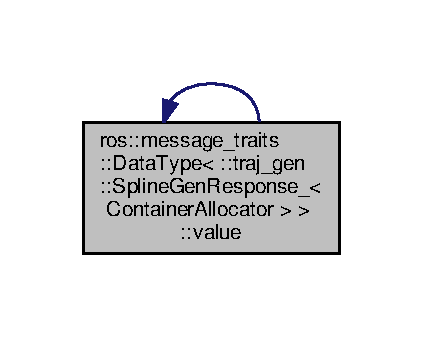
\includegraphics[width=203pt]{structros_1_1message__traits_1_1_data_type_3_01_1_1traj__gen_1_1_spline_gen_response___3_01_container_allocator_01_4_01_4_a45333b91e9108b4ab9094322fcc1243b_icgraph}
\end{center}
\end{figure}




The documentation for this struct was generated from the following file\+:\begin{DoxyCompactItemize}
\item 
build/devel/include/traj\+\_\+gen/\hyperlink{_spline_gen_response_8h}{Spline\+Gen\+Response.\+h}\end{DoxyCompactItemize}

\hypertarget{structros_1_1message__traits_1_1_definition_3_01_1_1traj__gen_1_1_poly_coeff___3_01_container_allocator_01_4_01_4}{}\section{ros\+:\+:message\+\_\+traits\+:\+:Definition$<$ \+:\+:traj\+\_\+gen\+:\+:Poly\+Coeff\+\_\+$<$ Container\+Allocator $>$ $>$ Struct Template Reference}
\label{structros_1_1message__traits_1_1_definition_3_01_1_1traj__gen_1_1_poly_coeff___3_01_container_allocator_01_4_01_4}\index{ros\+::message\+\_\+traits\+::\+Definition$<$ \+::traj\+\_\+gen\+::\+Poly\+Coeff\+\_\+$<$ Container\+Allocator $>$ $>$@{ros\+::message\+\_\+traits\+::\+Definition$<$ \+::traj\+\_\+gen\+::\+Poly\+Coeff\+\_\+$<$ Container\+Allocator $>$ $>$}}


{\ttfamily \#include $<$Poly\+Coeff.\+h$>$}

\subsection*{Static Public Member Functions}
\begin{DoxyCompactItemize}
\item 
static const char $\ast$ \hyperlink{structros_1_1message__traits_1_1_definition_3_01_1_1traj__gen_1_1_poly_coeff___3_01_container_allocator_01_4_01_4_abfeb944be80decc84a6964652ef522cf}{value} ()
\item 
static const char $\ast$ \hyperlink{structros_1_1message__traits_1_1_definition_3_01_1_1traj__gen_1_1_poly_coeff___3_01_container_allocator_01_4_01_4_a6cc5c00e3fd2db1f1877e717365cc341}{value} (const \+::\hyperlink{structtraj__gen_1_1_poly_coeff__}{traj\+\_\+gen\+::\+Poly\+Coeff\+\_\+}$<$ Container\+Allocator $>$ \&)
\end{DoxyCompactItemize}


\subsection{Detailed Description}
\subsubsection*{template$<$class Container\+Allocator$>$\\*
struct ros\+::message\+\_\+traits\+::\+Definition$<$ \+::traj\+\_\+gen\+::\+Poly\+Coeff\+\_\+$<$ Container\+Allocator $>$ $>$}



Definition at line 142 of file Poly\+Coeff.\+h.



\subsection{Member Function Documentation}
\index{ros\+::message\+\_\+traits\+::\+Definition$<$ \+::traj\+\_\+gen\+::\+Poly\+Coeff\+\_\+$<$ Container\+Allocator $>$ $>$@{ros\+::message\+\_\+traits\+::\+Definition$<$ \+::traj\+\_\+gen\+::\+Poly\+Coeff\+\_\+$<$ Container\+Allocator $>$ $>$}!value@{value}}
\index{value@{value}!ros\+::message\+\_\+traits\+::\+Definition$<$ \+::traj\+\_\+gen\+::\+Poly\+Coeff\+\_\+$<$ Container\+Allocator $>$ $>$@{ros\+::message\+\_\+traits\+::\+Definition$<$ \+::traj\+\_\+gen\+::\+Poly\+Coeff\+\_\+$<$ Container\+Allocator $>$ $>$}}
\subsubsection[{\texorpdfstring{value()}{value()}}]{\setlength{\rightskip}{0pt plus 5cm}template$<$class Container\+Allocator $>$ static const char$\ast$ ros\+::message\+\_\+traits\+::\+Definition$<$ \+::{\bf traj\+\_\+gen\+::\+Poly\+Coeff\+\_\+}$<$ Container\+Allocator $>$ $>$\+::value (
\begin{DoxyParamCaption}
{}
\end{DoxyParamCaption}
)\hspace{0.3cm}{\ttfamily [inline]}, {\ttfamily [static]}}\hypertarget{structros_1_1message__traits_1_1_definition_3_01_1_1traj__gen_1_1_poly_coeff___3_01_container_allocator_01_4_01_4_abfeb944be80decc84a6964652ef522cf}{}\label{structros_1_1message__traits_1_1_definition_3_01_1_1traj__gen_1_1_poly_coeff___3_01_container_allocator_01_4_01_4_abfeb944be80decc84a6964652ef522cf}


Definition at line 144 of file Poly\+Coeff.\+h.

\index{ros\+::message\+\_\+traits\+::\+Definition$<$ \+::traj\+\_\+gen\+::\+Poly\+Coeff\+\_\+$<$ Container\+Allocator $>$ $>$@{ros\+::message\+\_\+traits\+::\+Definition$<$ \+::traj\+\_\+gen\+::\+Poly\+Coeff\+\_\+$<$ Container\+Allocator $>$ $>$}!value@{value}}
\index{value@{value}!ros\+::message\+\_\+traits\+::\+Definition$<$ \+::traj\+\_\+gen\+::\+Poly\+Coeff\+\_\+$<$ Container\+Allocator $>$ $>$@{ros\+::message\+\_\+traits\+::\+Definition$<$ \+::traj\+\_\+gen\+::\+Poly\+Coeff\+\_\+$<$ Container\+Allocator $>$ $>$}}
\subsubsection[{\texorpdfstring{value(const \+::traj\+\_\+gen\+::\+Poly\+Coeff\+\_\+$<$ Container\+Allocator $>$ \&)}{value(const ::traj_gen::PolyCoeff_< ContainerAllocator > &)}}]{\setlength{\rightskip}{0pt plus 5cm}template$<$class Container\+Allocator $>$ static const char$\ast$ ros\+::message\+\_\+traits\+::\+Definition$<$ \+::{\bf traj\+\_\+gen\+::\+Poly\+Coeff\+\_\+}$<$ Container\+Allocator $>$ $>$\+::value (
\begin{DoxyParamCaption}
\item[{const \+::{\bf traj\+\_\+gen\+::\+Poly\+Coeff\+\_\+}$<$ Container\+Allocator $>$ \&}]{}
\end{DoxyParamCaption}
)\hspace{0.3cm}{\ttfamily [inline]}, {\ttfamily [static]}}\hypertarget{structros_1_1message__traits_1_1_definition_3_01_1_1traj__gen_1_1_poly_coeff___3_01_container_allocator_01_4_01_4_a6cc5c00e3fd2db1f1877e717365cc341}{}\label{structros_1_1message__traits_1_1_definition_3_01_1_1traj__gen_1_1_poly_coeff___3_01_container_allocator_01_4_01_4_a6cc5c00e3fd2db1f1877e717365cc341}


Definition at line 153 of file Poly\+Coeff.\+h.



Here is the call graph for this function\+:
\nopagebreak
\begin{figure}[H]
\begin{center}
\leavevmode
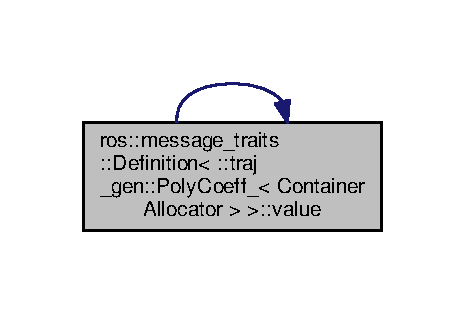
\includegraphics[width=223pt]{structros_1_1message__traits_1_1_definition_3_01_1_1traj__gen_1_1_poly_coeff___3_01_container_allocator_01_4_01_4_a6cc5c00e3fd2db1f1877e717365cc341_cgraph}
\end{center}
\end{figure}




Here is the caller graph for this function\+:
\nopagebreak
\begin{figure}[H]
\begin{center}
\leavevmode
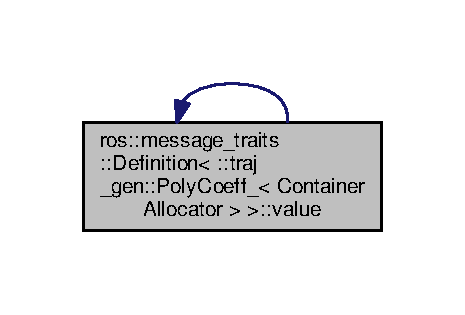
\includegraphics[width=223pt]{structros_1_1message__traits_1_1_definition_3_01_1_1traj__gen_1_1_poly_coeff___3_01_container_allocator_01_4_01_4_a6cc5c00e3fd2db1f1877e717365cc341_icgraph}
\end{center}
\end{figure}




The documentation for this struct was generated from the following file\+:\begin{DoxyCompactItemize}
\item 
build/devel/include/traj\+\_\+gen/\hyperlink{_poly_coeff_8h}{Poly\+Coeff.\+h}\end{DoxyCompactItemize}

\hypertarget{structros_1_1message__traits_1_1_definition_3_01_1_1traj__gen_1_1_poly_spline___3_01_container_allocator_01_4_01_4}{}\section{ros\+:\+:message\+\_\+traits\+:\+:Definition$<$ \+:\+:traj\+\_\+gen\+:\+:Poly\+Spline\+\_\+$<$ Container\+Allocator $>$ $>$ Struct Template Reference}
\label{structros_1_1message__traits_1_1_definition_3_01_1_1traj__gen_1_1_poly_spline___3_01_container_allocator_01_4_01_4}\index{ros\+::message\+\_\+traits\+::\+Definition$<$ \+::traj\+\_\+gen\+::\+Poly\+Spline\+\_\+$<$ Container\+Allocator $>$ $>$@{ros\+::message\+\_\+traits\+::\+Definition$<$ \+::traj\+\_\+gen\+::\+Poly\+Spline\+\_\+$<$ Container\+Allocator $>$ $>$}}


{\ttfamily \#include $<$Poly\+Spline.\+h$>$}

\subsection*{Static Public Member Functions}
\begin{DoxyCompactItemize}
\item 
static const char $\ast$ \hyperlink{structros_1_1message__traits_1_1_definition_3_01_1_1traj__gen_1_1_poly_spline___3_01_container_allocator_01_4_01_4_a0c5fafecad695d157aaa8804953a6b60}{value} ()
\item 
static const char $\ast$ \hyperlink{structros_1_1message__traits_1_1_definition_3_01_1_1traj__gen_1_1_poly_spline___3_01_container_allocator_01_4_01_4_aa8f178e3072c77bc6465e3e4ea27476b}{value} (const \+::\hyperlink{structtraj__gen_1_1_poly_spline__}{traj\+\_\+gen\+::\+Poly\+Spline\+\_\+}$<$ Container\+Allocator $>$ \&)
\end{DoxyCompactItemize}


\subsection{Detailed Description}
\subsubsection*{template$<$class Container\+Allocator$>$\\*
struct ros\+::message\+\_\+traits\+::\+Definition$<$ \+::traj\+\_\+gen\+::\+Poly\+Spline\+\_\+$<$ Container\+Allocator $>$ $>$}



Definition at line 153 of file Poly\+Spline.\+h.



\subsection{Member Function Documentation}
\index{ros\+::message\+\_\+traits\+::\+Definition$<$ \+::traj\+\_\+gen\+::\+Poly\+Spline\+\_\+$<$ Container\+Allocator $>$ $>$@{ros\+::message\+\_\+traits\+::\+Definition$<$ \+::traj\+\_\+gen\+::\+Poly\+Spline\+\_\+$<$ Container\+Allocator $>$ $>$}!value@{value}}
\index{value@{value}!ros\+::message\+\_\+traits\+::\+Definition$<$ \+::traj\+\_\+gen\+::\+Poly\+Spline\+\_\+$<$ Container\+Allocator $>$ $>$@{ros\+::message\+\_\+traits\+::\+Definition$<$ \+::traj\+\_\+gen\+::\+Poly\+Spline\+\_\+$<$ Container\+Allocator $>$ $>$}}
\subsubsection[{\texorpdfstring{value()}{value()}}]{\setlength{\rightskip}{0pt plus 5cm}template$<$class Container\+Allocator $>$ static const char$\ast$ ros\+::message\+\_\+traits\+::\+Definition$<$ \+::{\bf traj\+\_\+gen\+::\+Poly\+Spline\+\_\+}$<$ Container\+Allocator $>$ $>$\+::value (
\begin{DoxyParamCaption}
{}
\end{DoxyParamCaption}
)\hspace{0.3cm}{\ttfamily [inline]}, {\ttfamily [static]}}\hypertarget{structros_1_1message__traits_1_1_definition_3_01_1_1traj__gen_1_1_poly_spline___3_01_container_allocator_01_4_01_4_a0c5fafecad695d157aaa8804953a6b60}{}\label{structros_1_1message__traits_1_1_definition_3_01_1_1traj__gen_1_1_poly_spline___3_01_container_allocator_01_4_01_4_a0c5fafecad695d157aaa8804953a6b60}


Definition at line 155 of file Poly\+Spline.\+h.

\index{ros\+::message\+\_\+traits\+::\+Definition$<$ \+::traj\+\_\+gen\+::\+Poly\+Spline\+\_\+$<$ Container\+Allocator $>$ $>$@{ros\+::message\+\_\+traits\+::\+Definition$<$ \+::traj\+\_\+gen\+::\+Poly\+Spline\+\_\+$<$ Container\+Allocator $>$ $>$}!value@{value}}
\index{value@{value}!ros\+::message\+\_\+traits\+::\+Definition$<$ \+::traj\+\_\+gen\+::\+Poly\+Spline\+\_\+$<$ Container\+Allocator $>$ $>$@{ros\+::message\+\_\+traits\+::\+Definition$<$ \+::traj\+\_\+gen\+::\+Poly\+Spline\+\_\+$<$ Container\+Allocator $>$ $>$}}
\subsubsection[{\texorpdfstring{value(const \+::traj\+\_\+gen\+::\+Poly\+Spline\+\_\+$<$ Container\+Allocator $>$ \&)}{value(const ::traj_gen::PolySpline_< ContainerAllocator > &)}}]{\setlength{\rightskip}{0pt plus 5cm}template$<$class Container\+Allocator $>$ static const char$\ast$ ros\+::message\+\_\+traits\+::\+Definition$<$ \+::{\bf traj\+\_\+gen\+::\+Poly\+Spline\+\_\+}$<$ Container\+Allocator $>$ $>$\+::value (
\begin{DoxyParamCaption}
\item[{const \+::{\bf traj\+\_\+gen\+::\+Poly\+Spline\+\_\+}$<$ Container\+Allocator $>$ \&}]{}
\end{DoxyParamCaption}
)\hspace{0.3cm}{\ttfamily [inline]}, {\ttfamily [static]}}\hypertarget{structros_1_1message__traits_1_1_definition_3_01_1_1traj__gen_1_1_poly_spline___3_01_container_allocator_01_4_01_4_aa8f178e3072c77bc6465e3e4ea27476b}{}\label{structros_1_1message__traits_1_1_definition_3_01_1_1traj__gen_1_1_poly_spline___3_01_container_allocator_01_4_01_4_aa8f178e3072c77bc6465e3e4ea27476b}


Definition at line 173 of file Poly\+Spline.\+h.



Here is the call graph for this function\+:
\nopagebreak
\begin{figure}[H]
\begin{center}
\leavevmode
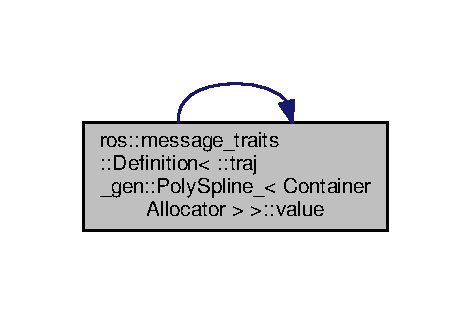
\includegraphics[width=226pt]{structros_1_1message__traits_1_1_definition_3_01_1_1traj__gen_1_1_poly_spline___3_01_container_allocator_01_4_01_4_aa8f178e3072c77bc6465e3e4ea27476b_cgraph}
\end{center}
\end{figure}




Here is the caller graph for this function\+:
\nopagebreak
\begin{figure}[H]
\begin{center}
\leavevmode
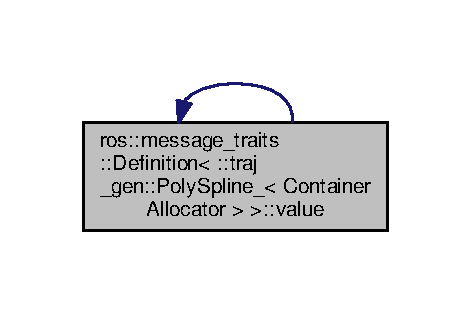
\includegraphics[width=226pt]{structros_1_1message__traits_1_1_definition_3_01_1_1traj__gen_1_1_poly_spline___3_01_container_allocator_01_4_01_4_aa8f178e3072c77bc6465e3e4ea27476b_icgraph}
\end{center}
\end{figure}




The documentation for this struct was generated from the following file\+:\begin{DoxyCompactItemize}
\item 
build/devel/include/traj\+\_\+gen/\hyperlink{_poly_spline_8h}{Poly\+Spline.\+h}\end{DoxyCompactItemize}

\hypertarget{structros_1_1message__traits_1_1_definition_3_01_1_1traj__gen_1_1_poly_spline_x_y_z___3_01_container_allocator_01_4_01_4}{}\section{ros\+:\+:message\+\_\+traits\+:\+:Definition$<$ \+:\+:traj\+\_\+gen\+:\+:Poly\+Spline\+X\+Y\+Z\+\_\+$<$ Container\+Allocator $>$ $>$ Struct Template Reference}
\label{structros_1_1message__traits_1_1_definition_3_01_1_1traj__gen_1_1_poly_spline_x_y_z___3_01_container_allocator_01_4_01_4}\index{ros\+::message\+\_\+traits\+::\+Definition$<$ \+::traj\+\_\+gen\+::\+Poly\+Spline\+X\+Y\+Z\+\_\+$<$ Container\+Allocator $>$ $>$@{ros\+::message\+\_\+traits\+::\+Definition$<$ \+::traj\+\_\+gen\+::\+Poly\+Spline\+X\+Y\+Z\+\_\+$<$ Container\+Allocator $>$ $>$}}


{\ttfamily \#include $<$Poly\+Spline\+X\+Y\+Z.\+h$>$}

\subsection*{Static Public Member Functions}
\begin{DoxyCompactItemize}
\item 
static const char $\ast$ \hyperlink{structros_1_1message__traits_1_1_definition_3_01_1_1traj__gen_1_1_poly_spline_x_y_z___3_01_container_allocator_01_4_01_4_a7b3cf44a2d6fb186d17c6f754fe9015a}{value} ()
\item 
static const char $\ast$ \hyperlink{structros_1_1message__traits_1_1_definition_3_01_1_1traj__gen_1_1_poly_spline_x_y_z___3_01_container_allocator_01_4_01_4_a87aa9969b0ea4241060c614e9b9231a7}{value} (const \+::\hyperlink{structtraj__gen_1_1_poly_spline_x_y_z__}{traj\+\_\+gen\+::\+Poly\+Spline\+X\+Y\+Z\+\_\+}$<$ Container\+Allocator $>$ \&)
\end{DoxyCompactItemize}


\subsection{Detailed Description}
\subsubsection*{template$<$class Container\+Allocator$>$\\*
struct ros\+::message\+\_\+traits\+::\+Definition$<$ \+::traj\+\_\+gen\+::\+Poly\+Spline\+X\+Y\+Z\+\_\+$<$ Container\+Allocator $>$ $>$}



Definition at line 170 of file Poly\+Spline\+X\+Y\+Z.\+h.



\subsection{Member Function Documentation}
\index{ros\+::message\+\_\+traits\+::\+Definition$<$ \+::traj\+\_\+gen\+::\+Poly\+Spline\+X\+Y\+Z\+\_\+$<$ Container\+Allocator $>$ $>$@{ros\+::message\+\_\+traits\+::\+Definition$<$ \+::traj\+\_\+gen\+::\+Poly\+Spline\+X\+Y\+Z\+\_\+$<$ Container\+Allocator $>$ $>$}!value@{value}}
\index{value@{value}!ros\+::message\+\_\+traits\+::\+Definition$<$ \+::traj\+\_\+gen\+::\+Poly\+Spline\+X\+Y\+Z\+\_\+$<$ Container\+Allocator $>$ $>$@{ros\+::message\+\_\+traits\+::\+Definition$<$ \+::traj\+\_\+gen\+::\+Poly\+Spline\+X\+Y\+Z\+\_\+$<$ Container\+Allocator $>$ $>$}}
\subsubsection[{\texorpdfstring{value()}{value()}}]{\setlength{\rightskip}{0pt plus 5cm}template$<$class Container\+Allocator $>$ static const char$\ast$ ros\+::message\+\_\+traits\+::\+Definition$<$ \+::{\bf traj\+\_\+gen\+::\+Poly\+Spline\+X\+Y\+Z\+\_\+}$<$ Container\+Allocator $>$ $>$\+::value (
\begin{DoxyParamCaption}
{}
\end{DoxyParamCaption}
)\hspace{0.3cm}{\ttfamily [inline]}, {\ttfamily [static]}}\hypertarget{structros_1_1message__traits_1_1_definition_3_01_1_1traj__gen_1_1_poly_spline_x_y_z___3_01_container_allocator_01_4_01_4_a7b3cf44a2d6fb186d17c6f754fe9015a}{}\label{structros_1_1message__traits_1_1_definition_3_01_1_1traj__gen_1_1_poly_spline_x_y_z___3_01_container_allocator_01_4_01_4_a7b3cf44a2d6fb186d17c6f754fe9015a}


Definition at line 172 of file Poly\+Spline\+X\+Y\+Z.\+h.

\index{ros\+::message\+\_\+traits\+::\+Definition$<$ \+::traj\+\_\+gen\+::\+Poly\+Spline\+X\+Y\+Z\+\_\+$<$ Container\+Allocator $>$ $>$@{ros\+::message\+\_\+traits\+::\+Definition$<$ \+::traj\+\_\+gen\+::\+Poly\+Spline\+X\+Y\+Z\+\_\+$<$ Container\+Allocator $>$ $>$}!value@{value}}
\index{value@{value}!ros\+::message\+\_\+traits\+::\+Definition$<$ \+::traj\+\_\+gen\+::\+Poly\+Spline\+X\+Y\+Z\+\_\+$<$ Container\+Allocator $>$ $>$@{ros\+::message\+\_\+traits\+::\+Definition$<$ \+::traj\+\_\+gen\+::\+Poly\+Spline\+X\+Y\+Z\+\_\+$<$ Container\+Allocator $>$ $>$}}
\subsubsection[{\texorpdfstring{value(const \+::traj\+\_\+gen\+::\+Poly\+Spline\+X\+Y\+Z\+\_\+$<$ Container\+Allocator $>$ \&)}{value(const ::traj_gen::PolySplineXYZ_< ContainerAllocator > &)}}]{\setlength{\rightskip}{0pt plus 5cm}template$<$class Container\+Allocator $>$ static const char$\ast$ ros\+::message\+\_\+traits\+::\+Definition$<$ \+::{\bf traj\+\_\+gen\+::\+Poly\+Spline\+X\+Y\+Z\+\_\+}$<$ Container\+Allocator $>$ $>$\+::value (
\begin{DoxyParamCaption}
\item[{const \+::{\bf traj\+\_\+gen\+::\+Poly\+Spline\+X\+Y\+Z\+\_\+}$<$ Container\+Allocator $>$ \&}]{}
\end{DoxyParamCaption}
)\hspace{0.3cm}{\ttfamily [inline]}, {\ttfamily [static]}}\hypertarget{structros_1_1message__traits_1_1_definition_3_01_1_1traj__gen_1_1_poly_spline_x_y_z___3_01_container_allocator_01_4_01_4_a87aa9969b0ea4241060c614e9b9231a7}{}\label{structros_1_1message__traits_1_1_definition_3_01_1_1traj__gen_1_1_poly_spline_x_y_z___3_01_container_allocator_01_4_01_4_a87aa9969b0ea4241060c614e9b9231a7}


Definition at line 200 of file Poly\+Spline\+X\+Y\+Z.\+h.



Here is the call graph for this function\+:
\nopagebreak
\begin{figure}[H]
\begin{center}
\leavevmode
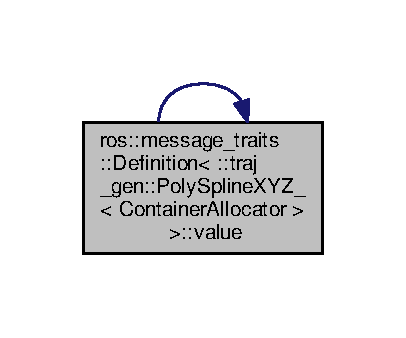
\includegraphics[width=195pt]{structros_1_1message__traits_1_1_definition_3_01_1_1traj__gen_1_1_poly_spline_x_y_z___3_01_container_allocator_01_4_01_4_a87aa9969b0ea4241060c614e9b9231a7_cgraph}
\end{center}
\end{figure}




Here is the caller graph for this function\+:
\nopagebreak
\begin{figure}[H]
\begin{center}
\leavevmode
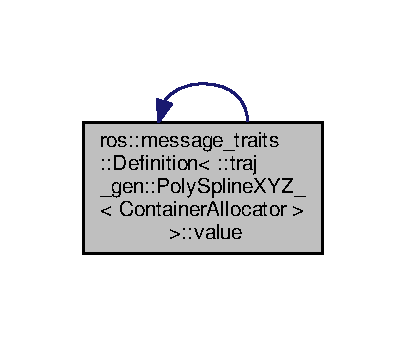
\includegraphics[width=195pt]{structros_1_1message__traits_1_1_definition_3_01_1_1traj__gen_1_1_poly_spline_x_y_z___3_01_container_allocator_01_4_01_4_a87aa9969b0ea4241060c614e9b9231a7_icgraph}
\end{center}
\end{figure}




The documentation for this struct was generated from the following file\+:\begin{DoxyCompactItemize}
\item 
build/devel/include/traj\+\_\+gen/\hyperlink{_poly_spline_x_y_z_8h}{Poly\+Spline\+X\+Y\+Z.\+h}\end{DoxyCompactItemize}

\hypertarget{structros_1_1message__traits_1_1_definition_3_01_1_1traj__gen_1_1_spline_gen_request___3_01_container_allocator_01_4_01_4}{}\section{ros\+:\+:message\+\_\+traits\+:\+:Definition$<$ \+:\+:traj\+\_\+gen\+:\+:Spline\+Gen\+Request\+\_\+$<$ Container\+Allocator $>$ $>$ Struct Template Reference}
\label{structros_1_1message__traits_1_1_definition_3_01_1_1traj__gen_1_1_spline_gen_request___3_01_container_allocator_01_4_01_4}\index{ros\+::message\+\_\+traits\+::\+Definition$<$ \+::traj\+\_\+gen\+::\+Spline\+Gen\+Request\+\_\+$<$ Container\+Allocator $>$ $>$@{ros\+::message\+\_\+traits\+::\+Definition$<$ \+::traj\+\_\+gen\+::\+Spline\+Gen\+Request\+\_\+$<$ Container\+Allocator $>$ $>$}}


{\ttfamily \#include $<$Spline\+Gen\+Request.\+h$>$}

\subsection*{Static Public Member Functions}
\begin{DoxyCompactItemize}
\item 
static const char $\ast$ \hyperlink{structros_1_1message__traits_1_1_definition_3_01_1_1traj__gen_1_1_spline_gen_request___3_01_container_allocator_01_4_01_4_a1c0e191fa6bd9645ab45f658864584d9}{value} ()
\item 
static const char $\ast$ \hyperlink{structros_1_1message__traits_1_1_definition_3_01_1_1traj__gen_1_1_spline_gen_request___3_01_container_allocator_01_4_01_4_a165a0952728f34e75639a65df1f2f57c}{value} (const \+::\hyperlink{structtraj__gen_1_1_spline_gen_request__}{traj\+\_\+gen\+::\+Spline\+Gen\+Request\+\_\+}$<$ Container\+Allocator $>$ \&)
\end{DoxyCompactItemize}


\subsection{Detailed Description}
\subsubsection*{template$<$class Container\+Allocator$>$\\*
struct ros\+::message\+\_\+traits\+::\+Definition$<$ \+::traj\+\_\+gen\+::\+Spline\+Gen\+Request\+\_\+$<$ Container\+Allocator $>$ $>$}



Definition at line 149 of file Spline\+Gen\+Request.\+h.



\subsection{Member Function Documentation}
\index{ros\+::message\+\_\+traits\+::\+Definition$<$ \+::traj\+\_\+gen\+::\+Spline\+Gen\+Request\+\_\+$<$ Container\+Allocator $>$ $>$@{ros\+::message\+\_\+traits\+::\+Definition$<$ \+::traj\+\_\+gen\+::\+Spline\+Gen\+Request\+\_\+$<$ Container\+Allocator $>$ $>$}!value@{value}}
\index{value@{value}!ros\+::message\+\_\+traits\+::\+Definition$<$ \+::traj\+\_\+gen\+::\+Spline\+Gen\+Request\+\_\+$<$ Container\+Allocator $>$ $>$@{ros\+::message\+\_\+traits\+::\+Definition$<$ \+::traj\+\_\+gen\+::\+Spline\+Gen\+Request\+\_\+$<$ Container\+Allocator $>$ $>$}}
\subsubsection[{\texorpdfstring{value()}{value()}}]{\setlength{\rightskip}{0pt plus 5cm}template$<$class Container\+Allocator $>$ static const char$\ast$ ros\+::message\+\_\+traits\+::\+Definition$<$ \+::{\bf traj\+\_\+gen\+::\+Spline\+Gen\+Request\+\_\+}$<$ Container\+Allocator $>$ $>$\+::value (
\begin{DoxyParamCaption}
{}
\end{DoxyParamCaption}
)\hspace{0.3cm}{\ttfamily [inline]}, {\ttfamily [static]}}\hypertarget{structros_1_1message__traits_1_1_definition_3_01_1_1traj__gen_1_1_spline_gen_request___3_01_container_allocator_01_4_01_4_a1c0e191fa6bd9645ab45f658864584d9}{}\label{structros_1_1message__traits_1_1_definition_3_01_1_1traj__gen_1_1_spline_gen_request___3_01_container_allocator_01_4_01_4_a1c0e191fa6bd9645ab45f658864584d9}


Definition at line 151 of file Spline\+Gen\+Request.\+h.

\index{ros\+::message\+\_\+traits\+::\+Definition$<$ \+::traj\+\_\+gen\+::\+Spline\+Gen\+Request\+\_\+$<$ Container\+Allocator $>$ $>$@{ros\+::message\+\_\+traits\+::\+Definition$<$ \+::traj\+\_\+gen\+::\+Spline\+Gen\+Request\+\_\+$<$ Container\+Allocator $>$ $>$}!value@{value}}
\index{value@{value}!ros\+::message\+\_\+traits\+::\+Definition$<$ \+::traj\+\_\+gen\+::\+Spline\+Gen\+Request\+\_\+$<$ Container\+Allocator $>$ $>$@{ros\+::message\+\_\+traits\+::\+Definition$<$ \+::traj\+\_\+gen\+::\+Spline\+Gen\+Request\+\_\+$<$ Container\+Allocator $>$ $>$}}
\subsubsection[{\texorpdfstring{value(const \+::traj\+\_\+gen\+::\+Spline\+Gen\+Request\+\_\+$<$ Container\+Allocator $>$ \&)}{value(const ::traj_gen::SplineGenRequest_< ContainerAllocator > &)}}]{\setlength{\rightskip}{0pt plus 5cm}template$<$class Container\+Allocator $>$ static const char$\ast$ ros\+::message\+\_\+traits\+::\+Definition$<$ \+::{\bf traj\+\_\+gen\+::\+Spline\+Gen\+Request\+\_\+}$<$ Container\+Allocator $>$ $>$\+::value (
\begin{DoxyParamCaption}
\item[{const \+::{\bf traj\+\_\+gen\+::\+Spline\+Gen\+Request\+\_\+}$<$ Container\+Allocator $>$ \&}]{}
\end{DoxyParamCaption}
)\hspace{0.3cm}{\ttfamily [inline]}, {\ttfamily [static]}}\hypertarget{structros_1_1message__traits_1_1_definition_3_01_1_1traj__gen_1_1_spline_gen_request___3_01_container_allocator_01_4_01_4_a165a0952728f34e75639a65df1f2f57c}{}\label{structros_1_1message__traits_1_1_definition_3_01_1_1traj__gen_1_1_spline_gen_request___3_01_container_allocator_01_4_01_4_a165a0952728f34e75639a65df1f2f57c}


Definition at line 229 of file Spline\+Gen\+Request.\+h.



Here is the call graph for this function\+:
\nopagebreak
\begin{figure}[H]
\begin{center}
\leavevmode
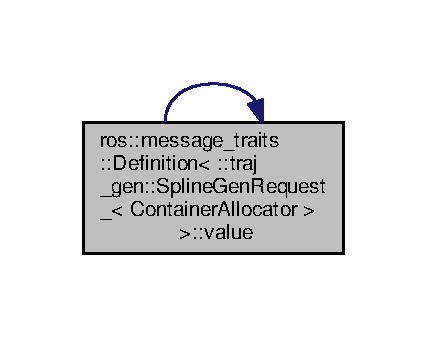
\includegraphics[width=205pt]{structros_1_1message__traits_1_1_definition_3_01_1_1traj__gen_1_1_spline_gen_request___3_01_container_allocator_01_4_01_4_a165a0952728f34e75639a65df1f2f57c_cgraph}
\end{center}
\end{figure}




Here is the caller graph for this function\+:
\nopagebreak
\begin{figure}[H]
\begin{center}
\leavevmode
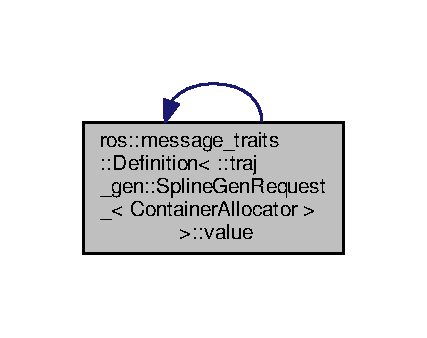
\includegraphics[width=205pt]{structros_1_1message__traits_1_1_definition_3_01_1_1traj__gen_1_1_spline_gen_request___3_01_container_allocator_01_4_01_4_a165a0952728f34e75639a65df1f2f57c_icgraph}
\end{center}
\end{figure}




The documentation for this struct was generated from the following file\+:\begin{DoxyCompactItemize}
\item 
build/devel/include/traj\+\_\+gen/\hyperlink{_spline_gen_request_8h}{Spline\+Gen\+Request.\+h}\end{DoxyCompactItemize}

\hypertarget{structros_1_1message__traits_1_1_definition_3_01_1_1traj__gen_1_1_spline_gen_response___3_01_container_allocator_01_4_01_4}{}\section{ros\+:\+:message\+\_\+traits\+:\+:Definition$<$ \+:\+:traj\+\_\+gen\+:\+:Spline\+Gen\+Response\+\_\+$<$ Container\+Allocator $>$ $>$ Struct Template Reference}
\label{structros_1_1message__traits_1_1_definition_3_01_1_1traj__gen_1_1_spline_gen_response___3_01_container_allocator_01_4_01_4}\index{ros\+::message\+\_\+traits\+::\+Definition$<$ \+::traj\+\_\+gen\+::\+Spline\+Gen\+Response\+\_\+$<$ Container\+Allocator $>$ $>$@{ros\+::message\+\_\+traits\+::\+Definition$<$ \+::traj\+\_\+gen\+::\+Spline\+Gen\+Response\+\_\+$<$ Container\+Allocator $>$ $>$}}


{\ttfamily \#include $<$Spline\+Gen\+Response.\+h$>$}

\subsection*{Static Public Member Functions}
\begin{DoxyCompactItemize}
\item 
static const char $\ast$ \hyperlink{structros_1_1message__traits_1_1_definition_3_01_1_1traj__gen_1_1_spline_gen_response___3_01_container_allocator_01_4_01_4_ac32fbb755c72ac9ec7185d4cca0bb481}{value} ()
\item 
static const char $\ast$ \hyperlink{structros_1_1message__traits_1_1_definition_3_01_1_1traj__gen_1_1_spline_gen_response___3_01_container_allocator_01_4_01_4_ae196e8f9afb8a1e90b1a408ecd8aca34}{value} (const \+::\hyperlink{structtraj__gen_1_1_spline_gen_response__}{traj\+\_\+gen\+::\+Spline\+Gen\+Response\+\_\+}$<$ Container\+Allocator $>$ \&)
\end{DoxyCompactItemize}


\subsection{Detailed Description}
\subsubsection*{template$<$class Container\+Allocator$>$\\*
struct ros\+::message\+\_\+traits\+::\+Definition$<$ \+::traj\+\_\+gen\+::\+Spline\+Gen\+Response\+\_\+$<$ Container\+Allocator $>$ $>$}



Definition at line 138 of file Spline\+Gen\+Response.\+h.



\subsection{Member Function Documentation}
\index{ros\+::message\+\_\+traits\+::\+Definition$<$ \+::traj\+\_\+gen\+::\+Spline\+Gen\+Response\+\_\+$<$ Container\+Allocator $>$ $>$@{ros\+::message\+\_\+traits\+::\+Definition$<$ \+::traj\+\_\+gen\+::\+Spline\+Gen\+Response\+\_\+$<$ Container\+Allocator $>$ $>$}!value@{value}}
\index{value@{value}!ros\+::message\+\_\+traits\+::\+Definition$<$ \+::traj\+\_\+gen\+::\+Spline\+Gen\+Response\+\_\+$<$ Container\+Allocator $>$ $>$@{ros\+::message\+\_\+traits\+::\+Definition$<$ \+::traj\+\_\+gen\+::\+Spline\+Gen\+Response\+\_\+$<$ Container\+Allocator $>$ $>$}}
\subsubsection[{\texorpdfstring{value()}{value()}}]{\setlength{\rightskip}{0pt plus 5cm}template$<$class Container\+Allocator $>$ static const char$\ast$ ros\+::message\+\_\+traits\+::\+Definition$<$ \+::{\bf traj\+\_\+gen\+::\+Spline\+Gen\+Response\+\_\+}$<$ Container\+Allocator $>$ $>$\+::value (
\begin{DoxyParamCaption}
{}
\end{DoxyParamCaption}
)\hspace{0.3cm}{\ttfamily [inline]}, {\ttfamily [static]}}\hypertarget{structros_1_1message__traits_1_1_definition_3_01_1_1traj__gen_1_1_spline_gen_response___3_01_container_allocator_01_4_01_4_ac32fbb755c72ac9ec7185d4cca0bb481}{}\label{structros_1_1message__traits_1_1_definition_3_01_1_1traj__gen_1_1_spline_gen_response___3_01_container_allocator_01_4_01_4_ac32fbb755c72ac9ec7185d4cca0bb481}


Definition at line 140 of file Spline\+Gen\+Response.\+h.

\index{ros\+::message\+\_\+traits\+::\+Definition$<$ \+::traj\+\_\+gen\+::\+Spline\+Gen\+Response\+\_\+$<$ Container\+Allocator $>$ $>$@{ros\+::message\+\_\+traits\+::\+Definition$<$ \+::traj\+\_\+gen\+::\+Spline\+Gen\+Response\+\_\+$<$ Container\+Allocator $>$ $>$}!value@{value}}
\index{value@{value}!ros\+::message\+\_\+traits\+::\+Definition$<$ \+::traj\+\_\+gen\+::\+Spline\+Gen\+Response\+\_\+$<$ Container\+Allocator $>$ $>$@{ros\+::message\+\_\+traits\+::\+Definition$<$ \+::traj\+\_\+gen\+::\+Spline\+Gen\+Response\+\_\+$<$ Container\+Allocator $>$ $>$}}
\subsubsection[{\texorpdfstring{value(const \+::traj\+\_\+gen\+::\+Spline\+Gen\+Response\+\_\+$<$ Container\+Allocator $>$ \&)}{value(const ::traj_gen::SplineGenResponse_< ContainerAllocator > &)}}]{\setlength{\rightskip}{0pt plus 5cm}template$<$class Container\+Allocator $>$ static const char$\ast$ ros\+::message\+\_\+traits\+::\+Definition$<$ \+::{\bf traj\+\_\+gen\+::\+Spline\+Gen\+Response\+\_\+}$<$ Container\+Allocator $>$ $>$\+::value (
\begin{DoxyParamCaption}
\item[{const \+::{\bf traj\+\_\+gen\+::\+Spline\+Gen\+Response\+\_\+}$<$ Container\+Allocator $>$ \&}]{}
\end{DoxyParamCaption}
)\hspace{0.3cm}{\ttfamily [inline]}, {\ttfamily [static]}}\hypertarget{structros_1_1message__traits_1_1_definition_3_01_1_1traj__gen_1_1_spline_gen_response___3_01_container_allocator_01_4_01_4_ae196e8f9afb8a1e90b1a408ecd8aca34}{}\label{structros_1_1message__traits_1_1_definition_3_01_1_1traj__gen_1_1_spline_gen_response___3_01_container_allocator_01_4_01_4_ae196e8f9afb8a1e90b1a408ecd8aca34}


Definition at line 173 of file Spline\+Gen\+Response.\+h.



Here is the call graph for this function\+:
\nopagebreak
\begin{figure}[H]
\begin{center}
\leavevmode
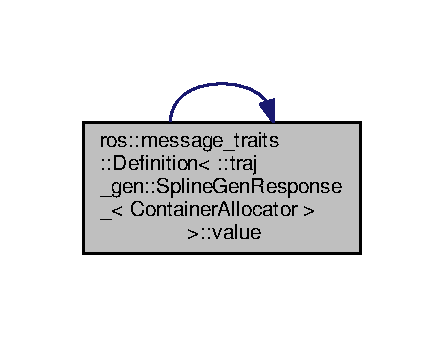
\includegraphics[width=213pt]{structros_1_1message__traits_1_1_definition_3_01_1_1traj__gen_1_1_spline_gen_response___3_01_container_allocator_01_4_01_4_ae196e8f9afb8a1e90b1a408ecd8aca34_cgraph}
\end{center}
\end{figure}




Here is the caller graph for this function\+:
\nopagebreak
\begin{figure}[H]
\begin{center}
\leavevmode
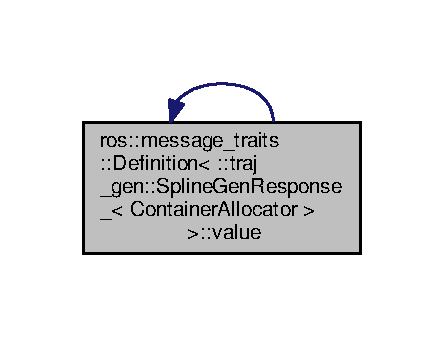
\includegraphics[width=213pt]{structros_1_1message__traits_1_1_definition_3_01_1_1traj__gen_1_1_spline_gen_response___3_01_container_allocator_01_4_01_4_ae196e8f9afb8a1e90b1a408ecd8aca34_icgraph}
\end{center}
\end{figure}




The documentation for this struct was generated from the following file\+:\begin{DoxyCompactItemize}
\item 
build/devel/include/traj\+\_\+gen/\hyperlink{_spline_gen_response_8h}{Spline\+Gen\+Response.\+h}\end{DoxyCompactItemize}

\hypertarget{structros_1_1message__traits_1_1_has_header_3_01_1_1traj__gen_1_1_poly_coeff___3_01_container_allocator_01_4_01_4}{}\section{ros\+:\+:message\+\_\+traits\+:\+:Has\+Header$<$ \+:\+:traj\+\_\+gen\+:\+:Poly\+Coeff\+\_\+$<$ Container\+Allocator $>$ $>$ Struct Template Reference}
\label{structros_1_1message__traits_1_1_has_header_3_01_1_1traj__gen_1_1_poly_coeff___3_01_container_allocator_01_4_01_4}\index{ros\+::message\+\_\+traits\+::\+Has\+Header$<$ \+::traj\+\_\+gen\+::\+Poly\+Coeff\+\_\+$<$ Container\+Allocator $>$ $>$@{ros\+::message\+\_\+traits\+::\+Has\+Header$<$ \+::traj\+\_\+gen\+::\+Poly\+Coeff\+\_\+$<$ Container\+Allocator $>$ $>$}}


{\ttfamily \#include $<$Poly\+Coeff.\+h$>$}



Inheritance diagram for ros\+:\+:message\+\_\+traits\+:\+:Has\+Header$<$ \+:\+:traj\+\_\+gen\+:\+:Poly\+Coeff\+\_\+$<$ Container\+Allocator $>$ $>$\+:
\nopagebreak
\begin{figure}[H]
\begin{center}
\leavevmode
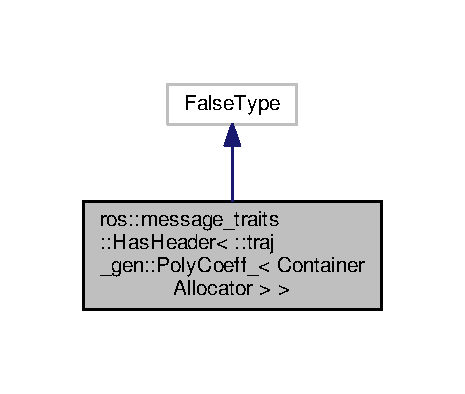
\includegraphics[width=223pt]{structros_1_1message__traits_1_1_has_header_3_01_1_1traj__gen_1_1_poly_coeff___3_01_container_aldf07fa77c346d7b11e48ed82ff9c3ca8}
\end{center}
\end{figure}


Collaboration diagram for ros\+:\+:message\+\_\+traits\+:\+:Has\+Header$<$ \+:\+:traj\+\_\+gen\+:\+:Poly\+Coeff\+\_\+$<$ Container\+Allocator $>$ $>$\+:
\nopagebreak
\begin{figure}[H]
\begin{center}
\leavevmode
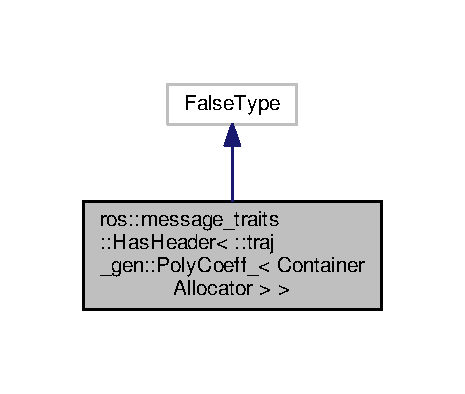
\includegraphics[width=223pt]{structros_1_1message__traits_1_1_has_header_3_01_1_1traj__gen_1_1_poly_coeff___3_01_container_allocator_01_4_01_4__coll__graph}
\end{center}
\end{figure}


\subsection{Detailed Description}
\subsubsection*{template$<$class Container\+Allocator$>$\\*
struct ros\+::message\+\_\+traits\+::\+Has\+Header$<$ \+::traj\+\_\+gen\+::\+Poly\+Coeff\+\_\+$<$ Container\+Allocator $>$ $>$}



Definition at line 107 of file Poly\+Coeff.\+h.



The documentation for this struct was generated from the following file\+:\begin{DoxyCompactItemize}
\item 
build/devel/include/traj\+\_\+gen/\hyperlink{_poly_coeff_8h}{Poly\+Coeff.\+h}\end{DoxyCompactItemize}

\hypertarget{structros_1_1message__traits_1_1_has_header_3_01_1_1traj__gen_1_1_poly_coeff___3_01_container_allocator_01_4_01const_01_01_4}{}\section{ros\+:\+:message\+\_\+traits\+:\+:Has\+Header$<$ \+:\+:traj\+\_\+gen\+:\+:Poly\+Coeff\+\_\+$<$ Container\+Allocator $>$ const $>$ Struct Template Reference}
\label{structros_1_1message__traits_1_1_has_header_3_01_1_1traj__gen_1_1_poly_coeff___3_01_container_allocator_01_4_01const_01_01_4}\index{ros\+::message\+\_\+traits\+::\+Has\+Header$<$ \+::traj\+\_\+gen\+::\+Poly\+Coeff\+\_\+$<$ Container\+Allocator $>$ const  $>$@{ros\+::message\+\_\+traits\+::\+Has\+Header$<$ \+::traj\+\_\+gen\+::\+Poly\+Coeff\+\_\+$<$ Container\+Allocator $>$ const  $>$}}


{\ttfamily \#include $<$Poly\+Coeff.\+h$>$}



Inheritance diagram for ros\+:\+:message\+\_\+traits\+:\+:Has\+Header$<$ \+:\+:traj\+\_\+gen\+:\+:Poly\+Coeff\+\_\+$<$ Container\+Allocator $>$ const $>$\+:
\nopagebreak
\begin{figure}[H]
\begin{center}
\leavevmode
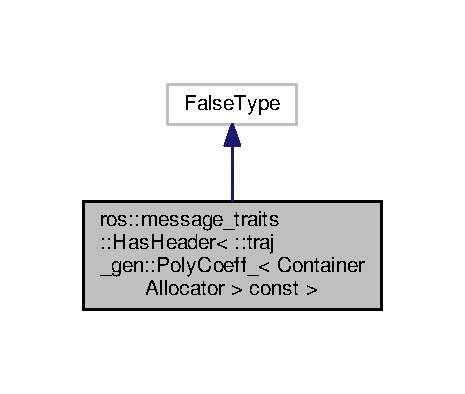
\includegraphics[width=223pt]{structros_1_1message__traits_1_1_has_header_3_01_1_1traj__gen_1_1_poly_coeff___3_01_container_al4a84c6fd39d6aaf2a154b726c28db8e0}
\end{center}
\end{figure}


Collaboration diagram for ros\+:\+:message\+\_\+traits\+:\+:Has\+Header$<$ \+:\+:traj\+\_\+gen\+:\+:Poly\+Coeff\+\_\+$<$ Container\+Allocator $>$ const $>$\+:
\nopagebreak
\begin{figure}[H]
\begin{center}
\leavevmode
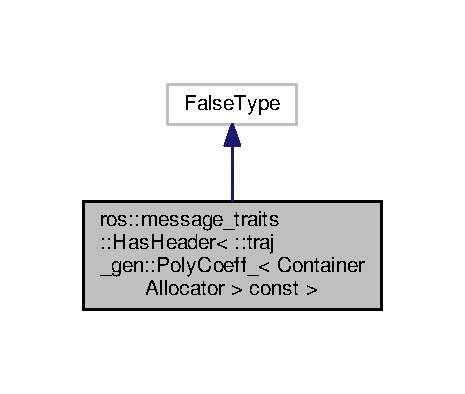
\includegraphics[width=223pt]{structros_1_1message__traits_1_1_has_header_3_01_1_1traj__gen_1_1_poly_coeff___3_01_container_alf58f4fe6cc8fa03dbaec520fad4b5243}
\end{center}
\end{figure}


\subsection{Detailed Description}
\subsubsection*{template$<$class Container\+Allocator$>$\\*
struct ros\+::message\+\_\+traits\+::\+Has\+Header$<$ \+::traj\+\_\+gen\+::\+Poly\+Coeff\+\_\+$<$ Container\+Allocator $>$ const  $>$}



Definition at line 112 of file Poly\+Coeff.\+h.



The documentation for this struct was generated from the following file\+:\begin{DoxyCompactItemize}
\item 
build/devel/include/traj\+\_\+gen/\hyperlink{_poly_coeff_8h}{Poly\+Coeff.\+h}\end{DoxyCompactItemize}

\hypertarget{structros_1_1message__traits_1_1_has_header_3_01_1_1traj__gen_1_1_poly_spline___3_01_container_allocator_01_4_01_4}{}\section{ros\+:\+:message\+\_\+traits\+:\+:Has\+Header$<$ \+:\+:traj\+\_\+gen\+:\+:Poly\+Spline\+\_\+$<$ Container\+Allocator $>$ $>$ Struct Template Reference}
\label{structros_1_1message__traits_1_1_has_header_3_01_1_1traj__gen_1_1_poly_spline___3_01_container_allocator_01_4_01_4}\index{ros\+::message\+\_\+traits\+::\+Has\+Header$<$ \+::traj\+\_\+gen\+::\+Poly\+Spline\+\_\+$<$ Container\+Allocator $>$ $>$@{ros\+::message\+\_\+traits\+::\+Has\+Header$<$ \+::traj\+\_\+gen\+::\+Poly\+Spline\+\_\+$<$ Container\+Allocator $>$ $>$}}


{\ttfamily \#include $<$Poly\+Spline.\+h$>$}



Inheritance diagram for ros\+:\+:message\+\_\+traits\+:\+:Has\+Header$<$ \+:\+:traj\+\_\+gen\+:\+:Poly\+Spline\+\_\+$<$ Container\+Allocator $>$ $>$\+:
\nopagebreak
\begin{figure}[H]
\begin{center}
\leavevmode
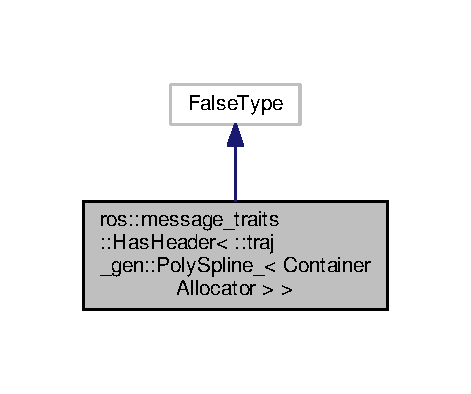
\includegraphics[width=226pt]{structros_1_1message__traits_1_1_has_header_3_01_1_1traj__gen_1_1_poly_spline___3_01_container_a0bd37295ce78e1f450c5afa4055212af}
\end{center}
\end{figure}


Collaboration diagram for ros\+:\+:message\+\_\+traits\+:\+:Has\+Header$<$ \+:\+:traj\+\_\+gen\+:\+:Poly\+Spline\+\_\+$<$ Container\+Allocator $>$ $>$\+:
\nopagebreak
\begin{figure}[H]
\begin{center}
\leavevmode
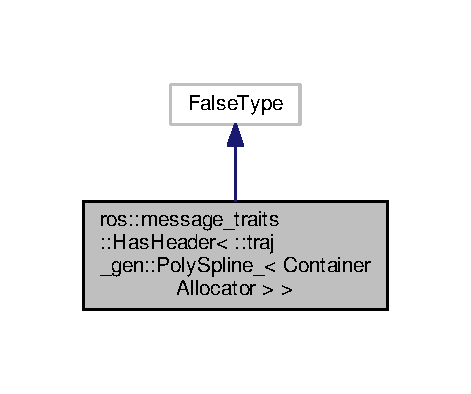
\includegraphics[width=226pt]{structros_1_1message__traits_1_1_has_header_3_01_1_1traj__gen_1_1_poly_spline___3_01_container_allocator_01_4_01_4__coll__graph}
\end{center}
\end{figure}


\subsection{Detailed Description}
\subsubsection*{template$<$class Container\+Allocator$>$\\*
struct ros\+::message\+\_\+traits\+::\+Has\+Header$<$ \+::traj\+\_\+gen\+::\+Poly\+Spline\+\_\+$<$ Container\+Allocator $>$ $>$}



Definition at line 118 of file Poly\+Spline.\+h.



The documentation for this struct was generated from the following file\+:\begin{DoxyCompactItemize}
\item 
build/devel/include/traj\+\_\+gen/\hyperlink{_poly_spline_8h}{Poly\+Spline.\+h}\end{DoxyCompactItemize}

\hypertarget{structros_1_1message__traits_1_1_has_header_3_01_1_1traj__gen_1_1_poly_spline___3_01_container_allocator_01_4_01const_01_01_4}{}\section{ros\+:\+:message\+\_\+traits\+:\+:Has\+Header$<$ \+:\+:traj\+\_\+gen\+:\+:Poly\+Spline\+\_\+$<$ Container\+Allocator $>$ const $>$ Struct Template Reference}
\label{structros_1_1message__traits_1_1_has_header_3_01_1_1traj__gen_1_1_poly_spline___3_01_container_allocator_01_4_01const_01_01_4}\index{ros\+::message\+\_\+traits\+::\+Has\+Header$<$ \+::traj\+\_\+gen\+::\+Poly\+Spline\+\_\+$<$ Container\+Allocator $>$ const  $>$@{ros\+::message\+\_\+traits\+::\+Has\+Header$<$ \+::traj\+\_\+gen\+::\+Poly\+Spline\+\_\+$<$ Container\+Allocator $>$ const  $>$}}


{\ttfamily \#include $<$Poly\+Spline.\+h$>$}



Inheritance diagram for ros\+:\+:message\+\_\+traits\+:\+:Has\+Header$<$ \+:\+:traj\+\_\+gen\+:\+:Poly\+Spline\+\_\+$<$ Container\+Allocator $>$ const $>$\+:
\nopagebreak
\begin{figure}[H]
\begin{center}
\leavevmode
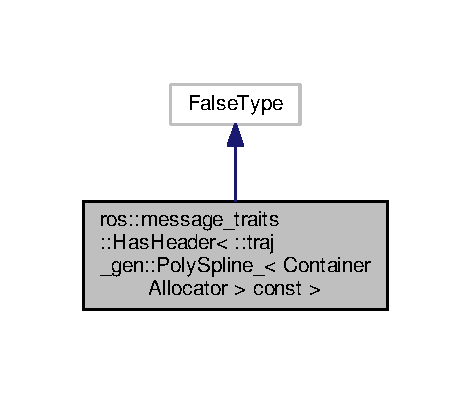
\includegraphics[width=226pt]{structros_1_1message__traits_1_1_has_header_3_01_1_1traj__gen_1_1_poly_spline___3_01_container_a0476a97252d1bf162707852ba289ac0f}
\end{center}
\end{figure}


Collaboration diagram for ros\+:\+:message\+\_\+traits\+:\+:Has\+Header$<$ \+:\+:traj\+\_\+gen\+:\+:Poly\+Spline\+\_\+$<$ Container\+Allocator $>$ const $>$\+:
\nopagebreak
\begin{figure}[H]
\begin{center}
\leavevmode
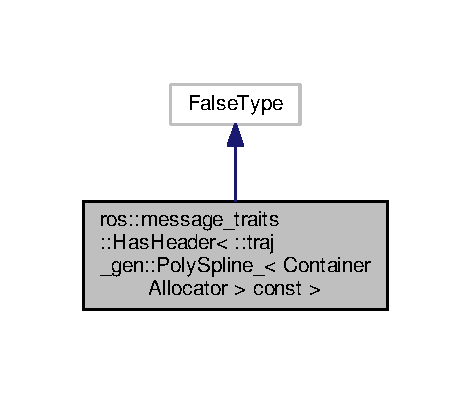
\includegraphics[width=226pt]{structros_1_1message__traits_1_1_has_header_3_01_1_1traj__gen_1_1_poly_spline___3_01_container_ab568bdcd624e6eff71fd54011c74493f}
\end{center}
\end{figure}


\subsection{Detailed Description}
\subsubsection*{template$<$class Container\+Allocator$>$\\*
struct ros\+::message\+\_\+traits\+::\+Has\+Header$<$ \+::traj\+\_\+gen\+::\+Poly\+Spline\+\_\+$<$ Container\+Allocator $>$ const  $>$}



Definition at line 123 of file Poly\+Spline.\+h.



The documentation for this struct was generated from the following file\+:\begin{DoxyCompactItemize}
\item 
build/devel/include/traj\+\_\+gen/\hyperlink{_poly_spline_8h}{Poly\+Spline.\+h}\end{DoxyCompactItemize}

\hypertarget{structros_1_1message__traits_1_1_has_header_3_01_1_1traj__gen_1_1_poly_spline_x_y_z___3_01_container_allocator_01_4_01_4}{}\section{ros\+:\+:message\+\_\+traits\+:\+:Has\+Header$<$ \+:\+:traj\+\_\+gen\+:\+:Poly\+Spline\+X\+Y\+Z\+\_\+$<$ Container\+Allocator $>$ $>$ Struct Template Reference}
\label{structros_1_1message__traits_1_1_has_header_3_01_1_1traj__gen_1_1_poly_spline_x_y_z___3_01_container_allocator_01_4_01_4}\index{ros\+::message\+\_\+traits\+::\+Has\+Header$<$ \+::traj\+\_\+gen\+::\+Poly\+Spline\+X\+Y\+Z\+\_\+$<$ Container\+Allocator $>$ $>$@{ros\+::message\+\_\+traits\+::\+Has\+Header$<$ \+::traj\+\_\+gen\+::\+Poly\+Spline\+X\+Y\+Z\+\_\+$<$ Container\+Allocator $>$ $>$}}


{\ttfamily \#include $<$Poly\+Spline\+X\+Y\+Z.\+h$>$}



Inheritance diagram for ros\+:\+:message\+\_\+traits\+:\+:Has\+Header$<$ \+:\+:traj\+\_\+gen\+:\+:Poly\+Spline\+X\+Y\+Z\+\_\+$<$ Container\+Allocator $>$ $>$\+:
\nopagebreak
\begin{figure}[H]
\begin{center}
\leavevmode
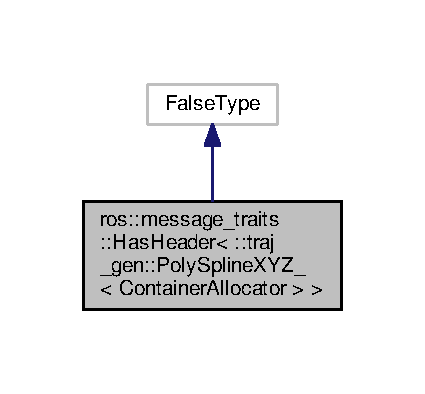
\includegraphics[width=204pt]{structros_1_1message__traits_1_1_has_header_3_01_1_1traj__gen_1_1_poly_spline_x_y_z___3_01_conta486bb23ba43f9f78140b01e7f046e5bb}
\end{center}
\end{figure}


Collaboration diagram for ros\+:\+:message\+\_\+traits\+:\+:Has\+Header$<$ \+:\+:traj\+\_\+gen\+:\+:Poly\+Spline\+X\+Y\+Z\+\_\+$<$ Container\+Allocator $>$ $>$\+:
\nopagebreak
\begin{figure}[H]
\begin{center}
\leavevmode
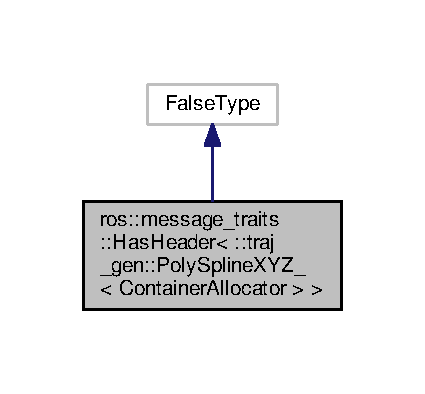
\includegraphics[width=204pt]{structros_1_1message__traits_1_1_has_header_3_01_1_1traj__gen_1_1_poly_spline_x_y_z___3_01_conta06f90fe96c801fa2e95cc1695f45131e}
\end{center}
\end{figure}


\subsection{Detailed Description}
\subsubsection*{template$<$class Container\+Allocator$>$\\*
struct ros\+::message\+\_\+traits\+::\+Has\+Header$<$ \+::traj\+\_\+gen\+::\+Poly\+Spline\+X\+Y\+Z\+\_\+$<$ Container\+Allocator $>$ $>$}



Definition at line 135 of file Poly\+Spline\+X\+Y\+Z.\+h.



The documentation for this struct was generated from the following file\+:\begin{DoxyCompactItemize}
\item 
build/devel/include/traj\+\_\+gen/\hyperlink{_poly_spline_x_y_z_8h}{Poly\+Spline\+X\+Y\+Z.\+h}\end{DoxyCompactItemize}

\hypertarget{structros_1_1message__traits_1_1_has_header_3_01_1_1traj__gen_1_1_poly_spline_x_y_z___3_01_conta12af5fbc53800516b6d924908e03fe26}{}\section{ros\+:\+:message\+\_\+traits\+:\+:Has\+Header$<$ \+:\+:traj\+\_\+gen\+:\+:Poly\+Spline\+X\+Y\+Z\+\_\+$<$ Container\+Allocator $>$ const $>$ Struct Template Reference}
\label{structros_1_1message__traits_1_1_has_header_3_01_1_1traj__gen_1_1_poly_spline_x_y_z___3_01_conta12af5fbc53800516b6d924908e03fe26}\index{ros\+::message\+\_\+traits\+::\+Has\+Header$<$ \+::traj\+\_\+gen\+::\+Poly\+Spline\+X\+Y\+Z\+\_\+$<$ Container\+Allocator $>$ const  $>$@{ros\+::message\+\_\+traits\+::\+Has\+Header$<$ \+::traj\+\_\+gen\+::\+Poly\+Spline\+X\+Y\+Z\+\_\+$<$ Container\+Allocator $>$ const  $>$}}


{\ttfamily \#include $<$Poly\+Spline\+X\+Y\+Z.\+h$>$}



Inheritance diagram for ros\+:\+:message\+\_\+traits\+:\+:Has\+Header$<$ \+:\+:traj\+\_\+gen\+:\+:Poly\+Spline\+X\+Y\+Z\+\_\+$<$ Container\+Allocator $>$ const $>$\+:
\nopagebreak
\begin{figure}[H]
\begin{center}
\leavevmode
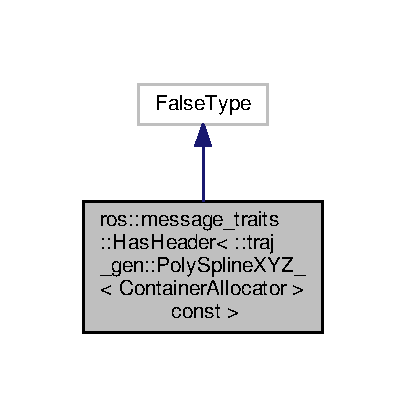
\includegraphics[width=195pt]{structros_1_1message__traits_1_1_has_header_3_01_1_1traj__gen_1_1_poly_spline_x_y_z___3_01_contaca21aef213def750e894585cb77d12cd}
\end{center}
\end{figure}


Collaboration diagram for ros\+:\+:message\+\_\+traits\+:\+:Has\+Header$<$ \+:\+:traj\+\_\+gen\+:\+:Poly\+Spline\+X\+Y\+Z\+\_\+$<$ Container\+Allocator $>$ const $>$\+:
\nopagebreak
\begin{figure}[H]
\begin{center}
\leavevmode
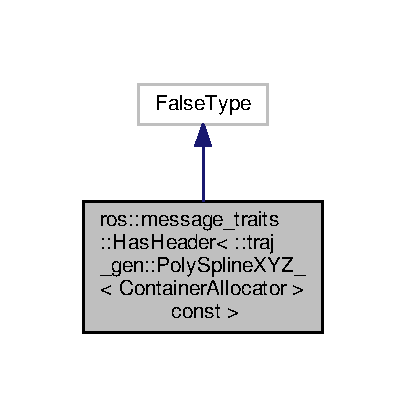
\includegraphics[width=195pt]{structros_1_1message__traits_1_1_has_header_3_01_1_1traj__gen_1_1_poly_spline_x_y_z___3_01_conta74a58fc55c4df1a71a08f6315e8e361f}
\end{center}
\end{figure}


\subsection{Detailed Description}
\subsubsection*{template$<$class Container\+Allocator$>$\\*
struct ros\+::message\+\_\+traits\+::\+Has\+Header$<$ \+::traj\+\_\+gen\+::\+Poly\+Spline\+X\+Y\+Z\+\_\+$<$ Container\+Allocator $>$ const  $>$}



Definition at line 140 of file Poly\+Spline\+X\+Y\+Z.\+h.



The documentation for this struct was generated from the following file\+:\begin{DoxyCompactItemize}
\item 
build/devel/include/traj\+\_\+gen/\hyperlink{_poly_spline_x_y_z_8h}{Poly\+Spline\+X\+Y\+Z.\+h}\end{DoxyCompactItemize}

\hypertarget{structros_1_1message__traits_1_1_has_header_3_01_1_1traj__gen_1_1_spline_gen_request___3_01_container_allocator_01_4_01_4}{}\section{ros\+:\+:message\+\_\+traits\+:\+:Has\+Header$<$ \+:\+:traj\+\_\+gen\+:\+:Spline\+Gen\+Request\+\_\+$<$ Container\+Allocator $>$ $>$ Struct Template Reference}
\label{structros_1_1message__traits_1_1_has_header_3_01_1_1traj__gen_1_1_spline_gen_request___3_01_container_allocator_01_4_01_4}\index{ros\+::message\+\_\+traits\+::\+Has\+Header$<$ \+::traj\+\_\+gen\+::\+Spline\+Gen\+Request\+\_\+$<$ Container\+Allocator $>$ $>$@{ros\+::message\+\_\+traits\+::\+Has\+Header$<$ \+::traj\+\_\+gen\+::\+Spline\+Gen\+Request\+\_\+$<$ Container\+Allocator $>$ $>$}}


{\ttfamily \#include $<$Spline\+Gen\+Request.\+h$>$}



Inheritance diagram for ros\+:\+:message\+\_\+traits\+:\+:Has\+Header$<$ \+:\+:traj\+\_\+gen\+:\+:Spline\+Gen\+Request\+\_\+$<$ Container\+Allocator $>$ $>$\+:
\nopagebreak
\begin{figure}[H]
\begin{center}
\leavevmode
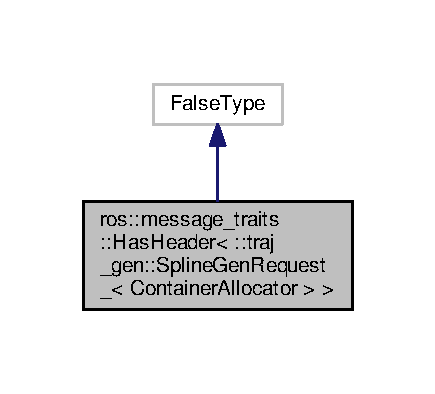
\includegraphics[width=209pt]{structros_1_1message__traits_1_1_has_header_3_01_1_1traj__gen_1_1_spline_gen_request___3_01_cont7253a3f63b7882e17703396bbd7a0011}
\end{center}
\end{figure}


Collaboration diagram for ros\+:\+:message\+\_\+traits\+:\+:Has\+Header$<$ \+:\+:traj\+\_\+gen\+:\+:Spline\+Gen\+Request\+\_\+$<$ Container\+Allocator $>$ $>$\+:
\nopagebreak
\begin{figure}[H]
\begin{center}
\leavevmode
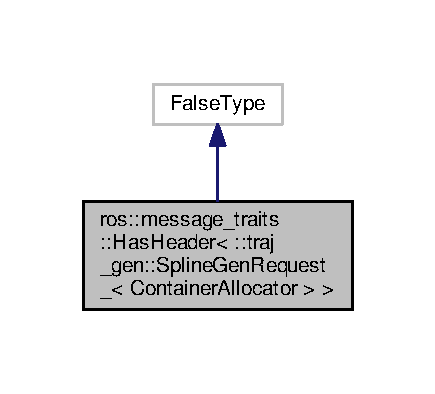
\includegraphics[width=209pt]{structros_1_1message__traits_1_1_has_header_3_01_1_1traj__gen_1_1_spline_gen_request___3_01_cont9f667a2e7d326dc7171383e50b237755}
\end{center}
\end{figure}


\subsection{Detailed Description}
\subsubsection*{template$<$class Container\+Allocator$>$\\*
struct ros\+::message\+\_\+traits\+::\+Has\+Header$<$ \+::traj\+\_\+gen\+::\+Spline\+Gen\+Request\+\_\+$<$ Container\+Allocator $>$ $>$}



Definition at line 114 of file Spline\+Gen\+Request.\+h.



The documentation for this struct was generated from the following file\+:\begin{DoxyCompactItemize}
\item 
build/devel/include/traj\+\_\+gen/\hyperlink{_spline_gen_request_8h}{Spline\+Gen\+Request.\+h}\end{DoxyCompactItemize}

\hypertarget{structros_1_1message__traits_1_1_has_header_3_01_1_1traj__gen_1_1_spline_gen_request___3_01_cont2d272e5e4f2aba4d565aef3b6188f511}{}\section{ros\+:\+:message\+\_\+traits\+:\+:Has\+Header$<$ \+:\+:traj\+\_\+gen\+:\+:Spline\+Gen\+Request\+\_\+$<$ Container\+Allocator $>$ const $>$ Struct Template Reference}
\label{structros_1_1message__traits_1_1_has_header_3_01_1_1traj__gen_1_1_spline_gen_request___3_01_cont2d272e5e4f2aba4d565aef3b6188f511}\index{ros\+::message\+\_\+traits\+::\+Has\+Header$<$ \+::traj\+\_\+gen\+::\+Spline\+Gen\+Request\+\_\+$<$ Container\+Allocator $>$ const  $>$@{ros\+::message\+\_\+traits\+::\+Has\+Header$<$ \+::traj\+\_\+gen\+::\+Spline\+Gen\+Request\+\_\+$<$ Container\+Allocator $>$ const  $>$}}


{\ttfamily \#include $<$Spline\+Gen\+Request.\+h$>$}



Inheritance diagram for ros\+:\+:message\+\_\+traits\+:\+:Has\+Header$<$ \+:\+:traj\+\_\+gen\+:\+:Spline\+Gen\+Request\+\_\+$<$ Container\+Allocator $>$ const $>$\+:
\nopagebreak
\begin{figure}[H]
\begin{center}
\leavevmode
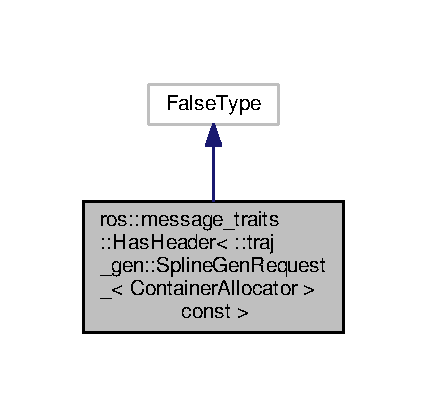
\includegraphics[width=205pt]{structros_1_1message__traits_1_1_has_header_3_01_1_1traj__gen_1_1_spline_gen_request___3_01_cont768eff21fd009d3bc1099511abeecb92}
\end{center}
\end{figure}


Collaboration diagram for ros\+:\+:message\+\_\+traits\+:\+:Has\+Header$<$ \+:\+:traj\+\_\+gen\+:\+:Spline\+Gen\+Request\+\_\+$<$ Container\+Allocator $>$ const $>$\+:
\nopagebreak
\begin{figure}[H]
\begin{center}
\leavevmode
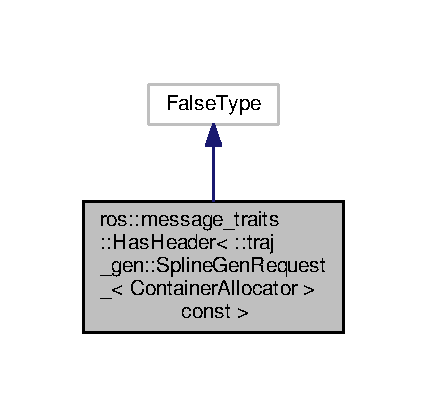
\includegraphics[width=205pt]{structros_1_1message__traits_1_1_has_header_3_01_1_1traj__gen_1_1_spline_gen_request___3_01_cont09eeeac25a1841f77cb680a359d6fe90}
\end{center}
\end{figure}


\subsection{Detailed Description}
\subsubsection*{template$<$class Container\+Allocator$>$\\*
struct ros\+::message\+\_\+traits\+::\+Has\+Header$<$ \+::traj\+\_\+gen\+::\+Spline\+Gen\+Request\+\_\+$<$ Container\+Allocator $>$ const  $>$}



Definition at line 119 of file Spline\+Gen\+Request.\+h.



The documentation for this struct was generated from the following file\+:\begin{DoxyCompactItemize}
\item 
build/devel/include/traj\+\_\+gen/\hyperlink{_spline_gen_request_8h}{Spline\+Gen\+Request.\+h}\end{DoxyCompactItemize}

\hypertarget{structros_1_1message__traits_1_1_has_header_3_01_1_1traj__gen_1_1_spline_gen_response___3_01_container_allocator_01_4_01_4}{}\section{ros\+:\+:message\+\_\+traits\+:\+:Has\+Header$<$ \+:\+:traj\+\_\+gen\+:\+:Spline\+Gen\+Response\+\_\+$<$ Container\+Allocator $>$ $>$ Struct Template Reference}
\label{structros_1_1message__traits_1_1_has_header_3_01_1_1traj__gen_1_1_spline_gen_response___3_01_container_allocator_01_4_01_4}\index{ros\+::message\+\_\+traits\+::\+Has\+Header$<$ \+::traj\+\_\+gen\+::\+Spline\+Gen\+Response\+\_\+$<$ Container\+Allocator $>$ $>$@{ros\+::message\+\_\+traits\+::\+Has\+Header$<$ \+::traj\+\_\+gen\+::\+Spline\+Gen\+Response\+\_\+$<$ Container\+Allocator $>$ $>$}}


{\ttfamily \#include $<$Spline\+Gen\+Response.\+h$>$}



Inheritance diagram for ros\+:\+:message\+\_\+traits\+:\+:Has\+Header$<$ \+:\+:traj\+\_\+gen\+:\+:Spline\+Gen\+Response\+\_\+$<$ Container\+Allocator $>$ $>$\+:
\nopagebreak
\begin{figure}[H]
\begin{center}
\leavevmode
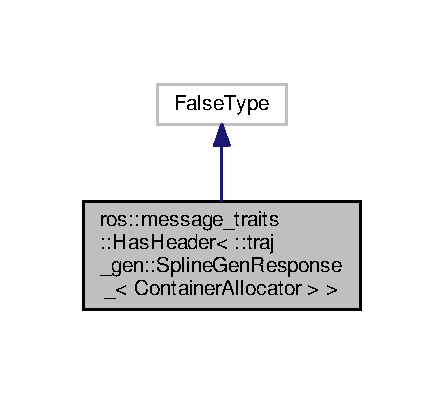
\includegraphics[width=213pt]{structros_1_1message__traits_1_1_has_header_3_01_1_1traj__gen_1_1_spline_gen_response___3_01_con5c49c447d1ccc9a13e503f523614e09c}
\end{center}
\end{figure}


Collaboration diagram for ros\+:\+:message\+\_\+traits\+:\+:Has\+Header$<$ \+:\+:traj\+\_\+gen\+:\+:Spline\+Gen\+Response\+\_\+$<$ Container\+Allocator $>$ $>$\+:
\nopagebreak
\begin{figure}[H]
\begin{center}
\leavevmode
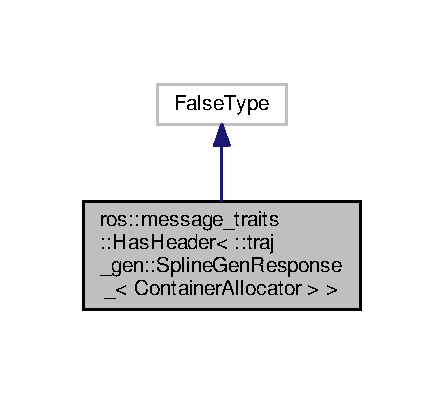
\includegraphics[width=213pt]{structros_1_1message__traits_1_1_has_header_3_01_1_1traj__gen_1_1_spline_gen_response___3_01_con0e8df4f2049cc64a66408ceeca784037}
\end{center}
\end{figure}


\subsection{Detailed Description}
\subsubsection*{template$<$class Container\+Allocator$>$\\*
struct ros\+::message\+\_\+traits\+::\+Has\+Header$<$ \+::traj\+\_\+gen\+::\+Spline\+Gen\+Response\+\_\+$<$ Container\+Allocator $>$ $>$}



Definition at line 103 of file Spline\+Gen\+Response.\+h.



The documentation for this struct was generated from the following file\+:\begin{DoxyCompactItemize}
\item 
build/devel/include/traj\+\_\+gen/\hyperlink{_spline_gen_response_8h}{Spline\+Gen\+Response.\+h}\end{DoxyCompactItemize}

\hypertarget{structros_1_1message__traits_1_1_has_header_3_01_1_1traj__gen_1_1_spline_gen_response___3_01_con1d0f3f08c39175b3253cd03ec47957a2}{}\section{ros\+:\+:message\+\_\+traits\+:\+:Has\+Header$<$ \+:\+:traj\+\_\+gen\+:\+:Spline\+Gen\+Response\+\_\+$<$ Container\+Allocator $>$ const $>$ Struct Template Reference}
\label{structros_1_1message__traits_1_1_has_header_3_01_1_1traj__gen_1_1_spline_gen_response___3_01_con1d0f3f08c39175b3253cd03ec47957a2}\index{ros\+::message\+\_\+traits\+::\+Has\+Header$<$ \+::traj\+\_\+gen\+::\+Spline\+Gen\+Response\+\_\+$<$ Container\+Allocator $>$ const  $>$@{ros\+::message\+\_\+traits\+::\+Has\+Header$<$ \+::traj\+\_\+gen\+::\+Spline\+Gen\+Response\+\_\+$<$ Container\+Allocator $>$ const  $>$}}


{\ttfamily \#include $<$Spline\+Gen\+Response.\+h$>$}



Inheritance diagram for ros\+:\+:message\+\_\+traits\+:\+:Has\+Header$<$ \+:\+:traj\+\_\+gen\+:\+:Spline\+Gen\+Response\+\_\+$<$ Container\+Allocator $>$ const $>$\+:
\nopagebreak
\begin{figure}[H]
\begin{center}
\leavevmode
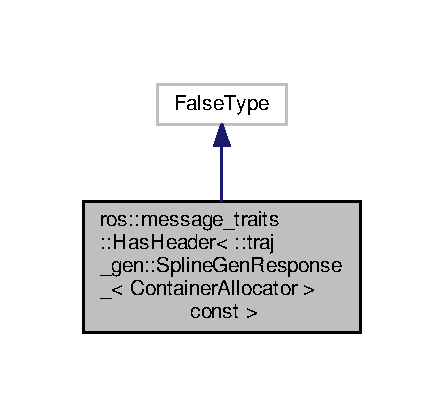
\includegraphics[width=213pt]{structros_1_1message__traits_1_1_has_header_3_01_1_1traj__gen_1_1_spline_gen_response___3_01_con7dfc813081338857bad60d02bb6992db}
\end{center}
\end{figure}


Collaboration diagram for ros\+:\+:message\+\_\+traits\+:\+:Has\+Header$<$ \+:\+:traj\+\_\+gen\+:\+:Spline\+Gen\+Response\+\_\+$<$ Container\+Allocator $>$ const $>$\+:
\nopagebreak
\begin{figure}[H]
\begin{center}
\leavevmode
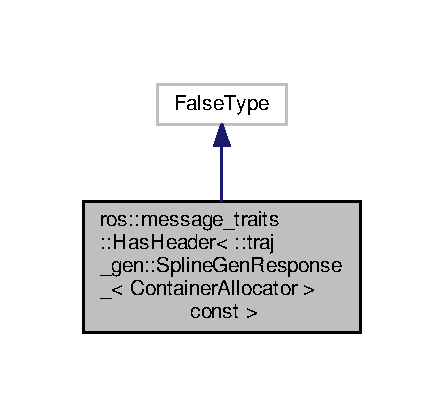
\includegraphics[width=213pt]{structros_1_1message__traits_1_1_has_header_3_01_1_1traj__gen_1_1_spline_gen_response___3_01_con2e598ba3f88ed72171ebcc30dc5d20c0}
\end{center}
\end{figure}


\subsection{Detailed Description}
\subsubsection*{template$<$class Container\+Allocator$>$\\*
struct ros\+::message\+\_\+traits\+::\+Has\+Header$<$ \+::traj\+\_\+gen\+::\+Spline\+Gen\+Response\+\_\+$<$ Container\+Allocator $>$ const  $>$}



Definition at line 108 of file Spline\+Gen\+Response.\+h.



The documentation for this struct was generated from the following file\+:\begin{DoxyCompactItemize}
\item 
build/devel/include/traj\+\_\+gen/\hyperlink{_spline_gen_response_8h}{Spline\+Gen\+Response.\+h}\end{DoxyCompactItemize}

\hypertarget{structros_1_1message__traits_1_1_is_fixed_size_3_01_1_1traj__gen_1_1_poly_coeff___3_01_container_allocator_01_4_01_4}{}\section{ros\+:\+:message\+\_\+traits\+:\+:Is\+Fixed\+Size$<$ \+:\+:traj\+\_\+gen\+:\+:Poly\+Coeff\+\_\+$<$ Container\+Allocator $>$ $>$ Struct Template Reference}
\label{structros_1_1message__traits_1_1_is_fixed_size_3_01_1_1traj__gen_1_1_poly_coeff___3_01_container_allocator_01_4_01_4}\index{ros\+::message\+\_\+traits\+::\+Is\+Fixed\+Size$<$ \+::traj\+\_\+gen\+::\+Poly\+Coeff\+\_\+$<$ Container\+Allocator $>$ $>$@{ros\+::message\+\_\+traits\+::\+Is\+Fixed\+Size$<$ \+::traj\+\_\+gen\+::\+Poly\+Coeff\+\_\+$<$ Container\+Allocator $>$ $>$}}


{\ttfamily \#include $<$Poly\+Coeff.\+h$>$}



Inheritance diagram for ros\+:\+:message\+\_\+traits\+:\+:Is\+Fixed\+Size$<$ \+:\+:traj\+\_\+gen\+:\+:Poly\+Coeff\+\_\+$<$ Container\+Allocator $>$ $>$\+:
\nopagebreak
\begin{figure}[H]
\begin{center}
\leavevmode
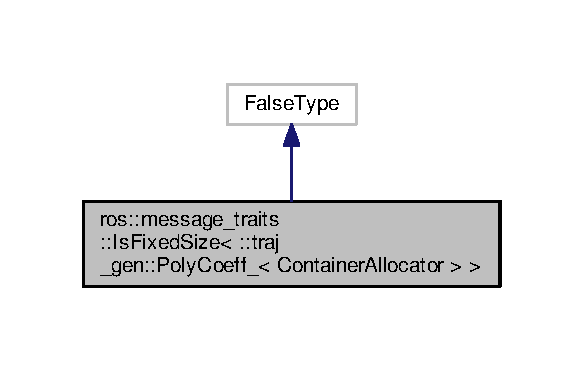
\includegraphics[width=280pt]{structros_1_1message__traits_1_1_is_fixed_size_3_01_1_1traj__gen_1_1_poly_coeff___3_01_container2d9ae7026b2181f5ee1c54bdb6a38e77}
\end{center}
\end{figure}


Collaboration diagram for ros\+:\+:message\+\_\+traits\+:\+:Is\+Fixed\+Size$<$ \+:\+:traj\+\_\+gen\+:\+:Poly\+Coeff\+\_\+$<$ Container\+Allocator $>$ $>$\+:
\nopagebreak
\begin{figure}[H]
\begin{center}
\leavevmode
\includegraphics[width=280pt]{structros_1_1message__traits_1_1_is_fixed_size_3_01_1_1traj__gen_1_1_poly_coeff___3_01_container9d922a5a6a4ffab143b153a23336fe47}
\end{center}
\end{figure}


\subsection{Detailed Description}
\subsubsection*{template$<$class Container\+Allocator$>$\\*
struct ros\+::message\+\_\+traits\+::\+Is\+Fixed\+Size$<$ \+::traj\+\_\+gen\+::\+Poly\+Coeff\+\_\+$<$ Container\+Allocator $>$ $>$}



Definition at line 87 of file Poly\+Coeff.\+h.



The documentation for this struct was generated from the following file\+:\begin{DoxyCompactItemize}
\item 
build/devel/include/traj\+\_\+gen/\hyperlink{_poly_coeff_8h}{Poly\+Coeff.\+h}\end{DoxyCompactItemize}

\hypertarget{structros_1_1message__traits_1_1_is_fixed_size_3_01_1_1traj__gen_1_1_poly_coeff___3_01_container_allocator_01_4_01const_01_01_4}{}\section{ros\+:\+:message\+\_\+traits\+:\+:Is\+Fixed\+Size$<$ \+:\+:traj\+\_\+gen\+:\+:Poly\+Coeff\+\_\+$<$ Container\+Allocator $>$ const $>$ Struct Template Reference}
\label{structros_1_1message__traits_1_1_is_fixed_size_3_01_1_1traj__gen_1_1_poly_coeff___3_01_container_allocator_01_4_01const_01_01_4}\index{ros\+::message\+\_\+traits\+::\+Is\+Fixed\+Size$<$ \+::traj\+\_\+gen\+::\+Poly\+Coeff\+\_\+$<$ Container\+Allocator $>$ const  $>$@{ros\+::message\+\_\+traits\+::\+Is\+Fixed\+Size$<$ \+::traj\+\_\+gen\+::\+Poly\+Coeff\+\_\+$<$ Container\+Allocator $>$ const  $>$}}


{\ttfamily \#include $<$Poly\+Coeff.\+h$>$}



Inheritance diagram for ros\+:\+:message\+\_\+traits\+:\+:Is\+Fixed\+Size$<$ \+:\+:traj\+\_\+gen\+:\+:Poly\+Coeff\+\_\+$<$ Container\+Allocator $>$ const $>$\+:
\nopagebreak
\begin{figure}[H]
\begin{center}
\leavevmode
\includegraphics[width=262pt]{structros_1_1message__traits_1_1_is_fixed_size_3_01_1_1traj__gen_1_1_poly_coeff___3_01_container85a4e372542c322523784d8a4d5c7075}
\end{center}
\end{figure}


Collaboration diagram for ros\+:\+:message\+\_\+traits\+:\+:Is\+Fixed\+Size$<$ \+:\+:traj\+\_\+gen\+:\+:Poly\+Coeff\+\_\+$<$ Container\+Allocator $>$ const $>$\+:
\nopagebreak
\begin{figure}[H]
\begin{center}
\leavevmode
\includegraphics[width=262pt]{structros_1_1message__traits_1_1_is_fixed_size_3_01_1_1traj__gen_1_1_poly_coeff___3_01_containerd5f8f91effdefc21ba19e7b7dd5811dc}
\end{center}
\end{figure}


\subsection{Detailed Description}
\subsubsection*{template$<$class Container\+Allocator$>$\\*
struct ros\+::message\+\_\+traits\+::\+Is\+Fixed\+Size$<$ \+::traj\+\_\+gen\+::\+Poly\+Coeff\+\_\+$<$ Container\+Allocator $>$ const  $>$}



Definition at line 92 of file Poly\+Coeff.\+h.



The documentation for this struct was generated from the following file\+:\begin{DoxyCompactItemize}
\item 
build/devel/include/traj\+\_\+gen/\hyperlink{_poly_coeff_8h}{Poly\+Coeff.\+h}\end{DoxyCompactItemize}

\hypertarget{structros_1_1message__traits_1_1_is_fixed_size_3_01_1_1traj__gen_1_1_poly_spline___3_01_container_allocator_01_4_01_4}{}\section{ros\+:\+:message\+\_\+traits\+:\+:Is\+Fixed\+Size$<$ \+:\+:traj\+\_\+gen\+:\+:Poly\+Spline\+\_\+$<$ Container\+Allocator $>$ $>$ Struct Template Reference}
\label{structros_1_1message__traits_1_1_is_fixed_size_3_01_1_1traj__gen_1_1_poly_spline___3_01_container_allocator_01_4_01_4}\index{ros\+::message\+\_\+traits\+::\+Is\+Fixed\+Size$<$ \+::traj\+\_\+gen\+::\+Poly\+Spline\+\_\+$<$ Container\+Allocator $>$ $>$@{ros\+::message\+\_\+traits\+::\+Is\+Fixed\+Size$<$ \+::traj\+\_\+gen\+::\+Poly\+Spline\+\_\+$<$ Container\+Allocator $>$ $>$}}


{\ttfamily \#include $<$Poly\+Spline.\+h$>$}



Inheritance diagram for ros\+:\+:message\+\_\+traits\+:\+:Is\+Fixed\+Size$<$ \+:\+:traj\+\_\+gen\+:\+:Poly\+Spline\+\_\+$<$ Container\+Allocator $>$ $>$\+:
\nopagebreak
\begin{figure}[H]
\begin{center}
\leavevmode
\includegraphics[width=226pt]{structros_1_1message__traits_1_1_is_fixed_size_3_01_1_1traj__gen_1_1_poly_spline___3_01_containe63526d3269ec5b55362cd2bba6a0012c}
\end{center}
\end{figure}


Collaboration diagram for ros\+:\+:message\+\_\+traits\+:\+:Is\+Fixed\+Size$<$ \+:\+:traj\+\_\+gen\+:\+:Poly\+Spline\+\_\+$<$ Container\+Allocator $>$ $>$\+:
\nopagebreak
\begin{figure}[H]
\begin{center}
\leavevmode
\includegraphics[width=226pt]{structros_1_1message__traits_1_1_is_fixed_size_3_01_1_1traj__gen_1_1_poly_spline___3_01_containe6604aea07d5fd1abd0408f875dd12872}
\end{center}
\end{figure}


\subsection{Detailed Description}
\subsubsection*{template$<$class Container\+Allocator$>$\\*
struct ros\+::message\+\_\+traits\+::\+Is\+Fixed\+Size$<$ \+::traj\+\_\+gen\+::\+Poly\+Spline\+\_\+$<$ Container\+Allocator $>$ $>$}



Definition at line 98 of file Poly\+Spline.\+h.



The documentation for this struct was generated from the following file\+:\begin{DoxyCompactItemize}
\item 
build/devel/include/traj\+\_\+gen/\hyperlink{_poly_spline_8h}{Poly\+Spline.\+h}\end{DoxyCompactItemize}

\hypertarget{structros_1_1message__traits_1_1_is_fixed_size_3_01_1_1traj__gen_1_1_poly_spline___3_01_containe7fdff08ae232c9034e9184a70d2080ac}{}\section{ros\+:\+:message\+\_\+traits\+:\+:Is\+Fixed\+Size$<$ \+:\+:traj\+\_\+gen\+:\+:Poly\+Spline\+\_\+$<$ Container\+Allocator $>$ const $>$ Struct Template Reference}
\label{structros_1_1message__traits_1_1_is_fixed_size_3_01_1_1traj__gen_1_1_poly_spline___3_01_containe7fdff08ae232c9034e9184a70d2080ac}\index{ros\+::message\+\_\+traits\+::\+Is\+Fixed\+Size$<$ \+::traj\+\_\+gen\+::\+Poly\+Spline\+\_\+$<$ Container\+Allocator $>$ const  $>$@{ros\+::message\+\_\+traits\+::\+Is\+Fixed\+Size$<$ \+::traj\+\_\+gen\+::\+Poly\+Spline\+\_\+$<$ Container\+Allocator $>$ const  $>$}}


{\ttfamily \#include $<$Poly\+Spline.\+h$>$}



Inheritance diagram for ros\+:\+:message\+\_\+traits\+:\+:Is\+Fixed\+Size$<$ \+:\+:traj\+\_\+gen\+:\+:Poly\+Spline\+\_\+$<$ Container\+Allocator $>$ const $>$\+:
\nopagebreak
\begin{figure}[H]
\begin{center}
\leavevmode
\includegraphics[width=226pt]{structros_1_1message__traits_1_1_is_fixed_size_3_01_1_1traj__gen_1_1_poly_spline___3_01_containe2ffa21fbf829e05347b72d9fb9c3a074}
\end{center}
\end{figure}


Collaboration diagram for ros\+:\+:message\+\_\+traits\+:\+:Is\+Fixed\+Size$<$ \+:\+:traj\+\_\+gen\+:\+:Poly\+Spline\+\_\+$<$ Container\+Allocator $>$ const $>$\+:
\nopagebreak
\begin{figure}[H]
\begin{center}
\leavevmode
\includegraphics[width=226pt]{structros_1_1message__traits_1_1_is_fixed_size_3_01_1_1traj__gen_1_1_poly_spline___3_01_containeb04f1af25e391d722db25c1ea289965c}
\end{center}
\end{figure}


\subsection{Detailed Description}
\subsubsection*{template$<$class Container\+Allocator$>$\\*
struct ros\+::message\+\_\+traits\+::\+Is\+Fixed\+Size$<$ \+::traj\+\_\+gen\+::\+Poly\+Spline\+\_\+$<$ Container\+Allocator $>$ const  $>$}



Definition at line 103 of file Poly\+Spline.\+h.



The documentation for this struct was generated from the following file\+:\begin{DoxyCompactItemize}
\item 
build/devel/include/traj\+\_\+gen/\hyperlink{_poly_spline_8h}{Poly\+Spline.\+h}\end{DoxyCompactItemize}

\hypertarget{structros_1_1message__traits_1_1_is_fixed_size_3_01_1_1traj__gen_1_1_poly_spline_x_y_z___3_01_container_allocator_01_4_01_4}{}\section{ros\+:\+:message\+\_\+traits\+:\+:Is\+Fixed\+Size$<$ \+:\+:traj\+\_\+gen\+:\+:Poly\+Spline\+X\+Y\+Z\+\_\+$<$ Container\+Allocator $>$ $>$ Struct Template Reference}
\label{structros_1_1message__traits_1_1_is_fixed_size_3_01_1_1traj__gen_1_1_poly_spline_x_y_z___3_01_container_allocator_01_4_01_4}\index{ros\+::message\+\_\+traits\+::\+Is\+Fixed\+Size$<$ \+::traj\+\_\+gen\+::\+Poly\+Spline\+X\+Y\+Z\+\_\+$<$ Container\+Allocator $>$ $>$@{ros\+::message\+\_\+traits\+::\+Is\+Fixed\+Size$<$ \+::traj\+\_\+gen\+::\+Poly\+Spline\+X\+Y\+Z\+\_\+$<$ Container\+Allocator $>$ $>$}}


{\ttfamily \#include $<$Poly\+Spline\+X\+Y\+Z.\+h$>$}



Inheritance diagram for ros\+:\+:message\+\_\+traits\+:\+:Is\+Fixed\+Size$<$ \+:\+:traj\+\_\+gen\+:\+:Poly\+Spline\+X\+Y\+Z\+\_\+$<$ Container\+Allocator $>$ $>$\+:
\nopagebreak
\begin{figure}[H]
\begin{center}
\leavevmode
\includegraphics[width=201pt]{structros_1_1message__traits_1_1_is_fixed_size_3_01_1_1traj__gen_1_1_poly_spline_x_y_z___3_01_cobbcc4722c4671c9c72a45e50c6d44bf0}
\end{center}
\end{figure}


Collaboration diagram for ros\+:\+:message\+\_\+traits\+:\+:Is\+Fixed\+Size$<$ \+:\+:traj\+\_\+gen\+:\+:Poly\+Spline\+X\+Y\+Z\+\_\+$<$ Container\+Allocator $>$ $>$\+:
\nopagebreak
\begin{figure}[H]
\begin{center}
\leavevmode
\includegraphics[width=201pt]{structros_1_1message__traits_1_1_is_fixed_size_3_01_1_1traj__gen_1_1_poly_spline_x_y_z___3_01_co6519299b09b1df68b3a2a6d06f00228c}
\end{center}
\end{figure}


\subsection{Detailed Description}
\subsubsection*{template$<$class Container\+Allocator$>$\\*
struct ros\+::message\+\_\+traits\+::\+Is\+Fixed\+Size$<$ \+::traj\+\_\+gen\+::\+Poly\+Spline\+X\+Y\+Z\+\_\+$<$ Container\+Allocator $>$ $>$}



Definition at line 115 of file Poly\+Spline\+X\+Y\+Z.\+h.



The documentation for this struct was generated from the following file\+:\begin{DoxyCompactItemize}
\item 
build/devel/include/traj\+\_\+gen/\hyperlink{_poly_spline_x_y_z_8h}{Poly\+Spline\+X\+Y\+Z.\+h}\end{DoxyCompactItemize}

\hypertarget{structros_1_1message__traits_1_1_is_fixed_size_3_01_1_1traj__gen_1_1_poly_spline_x_y_z___3_01_co1eebd7152468657d2fd84456c467c5f0}{}\section{ros\+:\+:message\+\_\+traits\+:\+:Is\+Fixed\+Size$<$ \+:\+:traj\+\_\+gen\+:\+:Poly\+Spline\+X\+Y\+Z\+\_\+$<$ Container\+Allocator $>$ const $>$ Struct Template Reference}
\label{structros_1_1message__traits_1_1_is_fixed_size_3_01_1_1traj__gen_1_1_poly_spline_x_y_z___3_01_co1eebd7152468657d2fd84456c467c5f0}\index{ros\+::message\+\_\+traits\+::\+Is\+Fixed\+Size$<$ \+::traj\+\_\+gen\+::\+Poly\+Spline\+X\+Y\+Z\+\_\+$<$ Container\+Allocator $>$ const  $>$@{ros\+::message\+\_\+traits\+::\+Is\+Fixed\+Size$<$ \+::traj\+\_\+gen\+::\+Poly\+Spline\+X\+Y\+Z\+\_\+$<$ Container\+Allocator $>$ const  $>$}}


{\ttfamily \#include $<$Poly\+Spline\+X\+Y\+Z.\+h$>$}



Inheritance diagram for ros\+:\+:message\+\_\+traits\+:\+:Is\+Fixed\+Size$<$ \+:\+:traj\+\_\+gen\+:\+:Poly\+Spline\+X\+Y\+Z\+\_\+$<$ Container\+Allocator $>$ const $>$\+:
\nopagebreak
\begin{figure}[H]
\begin{center}
\leavevmode
\includegraphics[width=225pt]{structros_1_1message__traits_1_1_is_fixed_size_3_01_1_1traj__gen_1_1_poly_spline_x_y_z___3_01_co3b183c5d0e8c16bf36fbbad146c3e637}
\end{center}
\end{figure}


Collaboration diagram for ros\+:\+:message\+\_\+traits\+:\+:Is\+Fixed\+Size$<$ \+:\+:traj\+\_\+gen\+:\+:Poly\+Spline\+X\+Y\+Z\+\_\+$<$ Container\+Allocator $>$ const $>$\+:
\nopagebreak
\begin{figure}[H]
\begin{center}
\leavevmode
\includegraphics[width=225pt]{structros_1_1message__traits_1_1_is_fixed_size_3_01_1_1traj__gen_1_1_poly_spline_x_y_z___3_01_co84c2177a97b867b5dd621cd15fcdebb5}
\end{center}
\end{figure}


\subsection{Detailed Description}
\subsubsection*{template$<$class Container\+Allocator$>$\\*
struct ros\+::message\+\_\+traits\+::\+Is\+Fixed\+Size$<$ \+::traj\+\_\+gen\+::\+Poly\+Spline\+X\+Y\+Z\+\_\+$<$ Container\+Allocator $>$ const  $>$}



Definition at line 120 of file Poly\+Spline\+X\+Y\+Z.\+h.



The documentation for this struct was generated from the following file\+:\begin{DoxyCompactItemize}
\item 
build/devel/include/traj\+\_\+gen/\hyperlink{_poly_spline_x_y_z_8h}{Poly\+Spline\+X\+Y\+Z.\+h}\end{DoxyCompactItemize}

\hypertarget{structros_1_1message__traits_1_1_is_fixed_size_3_01_1_1traj__gen_1_1_spline_gen_request___3_01_container_allocator_01_4_01_4}{}\section{ros\+:\+:message\+\_\+traits\+:\+:Is\+Fixed\+Size$<$ \+:\+:traj\+\_\+gen\+:\+:Spline\+Gen\+Request\+\_\+$<$ Container\+Allocator $>$ $>$ Struct Template Reference}
\label{structros_1_1message__traits_1_1_is_fixed_size_3_01_1_1traj__gen_1_1_spline_gen_request___3_01_container_allocator_01_4_01_4}\index{ros\+::message\+\_\+traits\+::\+Is\+Fixed\+Size$<$ \+::traj\+\_\+gen\+::\+Spline\+Gen\+Request\+\_\+$<$ Container\+Allocator $>$ $>$@{ros\+::message\+\_\+traits\+::\+Is\+Fixed\+Size$<$ \+::traj\+\_\+gen\+::\+Spline\+Gen\+Request\+\_\+$<$ Container\+Allocator $>$ $>$}}


{\ttfamily \#include $<$Spline\+Gen\+Request.\+h$>$}



Inheritance diagram for ros\+:\+:message\+\_\+traits\+:\+:Is\+Fixed\+Size$<$ \+:\+:traj\+\_\+gen\+:\+:Spline\+Gen\+Request\+\_\+$<$ Container\+Allocator $>$ $>$\+:
\nopagebreak
\begin{figure}[H]
\begin{center}
\leavevmode
\includegraphics[width=209pt]{structros_1_1message__traits_1_1_is_fixed_size_3_01_1_1traj__gen_1_1_spline_gen_request___3_01_c17f4ce088c1755e05f9dd27d81ef5372}
\end{center}
\end{figure}


Collaboration diagram for ros\+:\+:message\+\_\+traits\+:\+:Is\+Fixed\+Size$<$ \+:\+:traj\+\_\+gen\+:\+:Spline\+Gen\+Request\+\_\+$<$ Container\+Allocator $>$ $>$\+:
\nopagebreak
\begin{figure}[H]
\begin{center}
\leavevmode
\includegraphics[width=209pt]{structros_1_1message__traits_1_1_is_fixed_size_3_01_1_1traj__gen_1_1_spline_gen_request___3_01_cc231b5d5b6d62c31637ff0c472239a25}
\end{center}
\end{figure}


\subsection{Detailed Description}
\subsubsection*{template$<$class Container\+Allocator$>$\\*
struct ros\+::message\+\_\+traits\+::\+Is\+Fixed\+Size$<$ \+::traj\+\_\+gen\+::\+Spline\+Gen\+Request\+\_\+$<$ Container\+Allocator $>$ $>$}



Definition at line 94 of file Spline\+Gen\+Request.\+h.



The documentation for this struct was generated from the following file\+:\begin{DoxyCompactItemize}
\item 
build/devel/include/traj\+\_\+gen/\hyperlink{_spline_gen_request_8h}{Spline\+Gen\+Request.\+h}\end{DoxyCompactItemize}

\hypertarget{structros_1_1message__traits_1_1_is_fixed_size_3_01_1_1traj__gen_1_1_spline_gen_request___3_01_c1ecde96b449db99fe3c628d37e48a8e1}{}\section{ros\+:\+:message\+\_\+traits\+:\+:Is\+Fixed\+Size$<$ \+:\+:traj\+\_\+gen\+:\+:Spline\+Gen\+Request\+\_\+$<$ Container\+Allocator $>$ const $>$ Struct Template Reference}
\label{structros_1_1message__traits_1_1_is_fixed_size_3_01_1_1traj__gen_1_1_spline_gen_request___3_01_c1ecde96b449db99fe3c628d37e48a8e1}\index{ros\+::message\+\_\+traits\+::\+Is\+Fixed\+Size$<$ \+::traj\+\_\+gen\+::\+Spline\+Gen\+Request\+\_\+$<$ Container\+Allocator $>$ const  $>$@{ros\+::message\+\_\+traits\+::\+Is\+Fixed\+Size$<$ \+::traj\+\_\+gen\+::\+Spline\+Gen\+Request\+\_\+$<$ Container\+Allocator $>$ const  $>$}}


{\ttfamily \#include $<$Spline\+Gen\+Request.\+h$>$}



Inheritance diagram for ros\+:\+:message\+\_\+traits\+:\+:Is\+Fixed\+Size$<$ \+:\+:traj\+\_\+gen\+:\+:Spline\+Gen\+Request\+\_\+$<$ Container\+Allocator $>$ const $>$\+:
\nopagebreak
\begin{figure}[H]
\begin{center}
\leavevmode
\includegraphics[width=205pt]{structros_1_1message__traits_1_1_is_fixed_size_3_01_1_1traj__gen_1_1_spline_gen_request___3_01_cd32f4725f181f55e36c235be2ba6f31a}
\end{center}
\end{figure}


Collaboration diagram for ros\+:\+:message\+\_\+traits\+:\+:Is\+Fixed\+Size$<$ \+:\+:traj\+\_\+gen\+:\+:Spline\+Gen\+Request\+\_\+$<$ Container\+Allocator $>$ const $>$\+:
\nopagebreak
\begin{figure}[H]
\begin{center}
\leavevmode
\includegraphics[width=205pt]{structros_1_1message__traits_1_1_is_fixed_size_3_01_1_1traj__gen_1_1_spline_gen_request___3_01_c930820b086f8eab35380ecf895fcf257}
\end{center}
\end{figure}


\subsection{Detailed Description}
\subsubsection*{template$<$class Container\+Allocator$>$\\*
struct ros\+::message\+\_\+traits\+::\+Is\+Fixed\+Size$<$ \+::traj\+\_\+gen\+::\+Spline\+Gen\+Request\+\_\+$<$ Container\+Allocator $>$ const  $>$}



Definition at line 99 of file Spline\+Gen\+Request.\+h.



The documentation for this struct was generated from the following file\+:\begin{DoxyCompactItemize}
\item 
build/devel/include/traj\+\_\+gen/\hyperlink{_spline_gen_request_8h}{Spline\+Gen\+Request.\+h}\end{DoxyCompactItemize}

\hypertarget{structros_1_1message__traits_1_1_is_fixed_size_3_01_1_1traj__gen_1_1_spline_gen_response___3_01_container_allocator_01_4_01_4}{}\section{ros\+:\+:message\+\_\+traits\+:\+:Is\+Fixed\+Size$<$ \+:\+:traj\+\_\+gen\+:\+:Spline\+Gen\+Response\+\_\+$<$ Container\+Allocator $>$ $>$ Struct Template Reference}
\label{structros_1_1message__traits_1_1_is_fixed_size_3_01_1_1traj__gen_1_1_spline_gen_response___3_01_container_allocator_01_4_01_4}\index{ros\+::message\+\_\+traits\+::\+Is\+Fixed\+Size$<$ \+::traj\+\_\+gen\+::\+Spline\+Gen\+Response\+\_\+$<$ Container\+Allocator $>$ $>$@{ros\+::message\+\_\+traits\+::\+Is\+Fixed\+Size$<$ \+::traj\+\_\+gen\+::\+Spline\+Gen\+Response\+\_\+$<$ Container\+Allocator $>$ $>$}}


{\ttfamily \#include $<$Spline\+Gen\+Response.\+h$>$}



Inheritance diagram for ros\+:\+:message\+\_\+traits\+:\+:Is\+Fixed\+Size$<$ \+:\+:traj\+\_\+gen\+:\+:Spline\+Gen\+Response\+\_\+$<$ Container\+Allocator $>$ $>$\+:
\nopagebreak
\begin{figure}[H]
\begin{center}
\leavevmode
\includegraphics[width=213pt]{structros_1_1message__traits_1_1_is_fixed_size_3_01_1_1traj__gen_1_1_spline_gen_response___3_01_9973154c99bc97e2826b3b97addf2cad}
\end{center}
\end{figure}


Collaboration diagram for ros\+:\+:message\+\_\+traits\+:\+:Is\+Fixed\+Size$<$ \+:\+:traj\+\_\+gen\+:\+:Spline\+Gen\+Response\+\_\+$<$ Container\+Allocator $>$ $>$\+:
\nopagebreak
\begin{figure}[H]
\begin{center}
\leavevmode
\includegraphics[width=213pt]{structros_1_1message__traits_1_1_is_fixed_size_3_01_1_1traj__gen_1_1_spline_gen_response___3_01_541b5f3e958d29158a93d0c7c8bdbc12}
\end{center}
\end{figure}


\subsection{Detailed Description}
\subsubsection*{template$<$class Container\+Allocator$>$\\*
struct ros\+::message\+\_\+traits\+::\+Is\+Fixed\+Size$<$ \+::traj\+\_\+gen\+::\+Spline\+Gen\+Response\+\_\+$<$ Container\+Allocator $>$ $>$}



Definition at line 83 of file Spline\+Gen\+Response.\+h.



The documentation for this struct was generated from the following file\+:\begin{DoxyCompactItemize}
\item 
build/devel/include/traj\+\_\+gen/\hyperlink{_spline_gen_response_8h}{Spline\+Gen\+Response.\+h}\end{DoxyCompactItemize}

\hypertarget{structros_1_1message__traits_1_1_is_fixed_size_3_01_1_1traj__gen_1_1_spline_gen_response___3_01_2336c611429bfb59739e76b3c3f70a28}{}\section{ros\+:\+:message\+\_\+traits\+:\+:Is\+Fixed\+Size$<$ \+:\+:traj\+\_\+gen\+:\+:Spline\+Gen\+Response\+\_\+$<$ Container\+Allocator $>$ const $>$ Struct Template Reference}
\label{structros_1_1message__traits_1_1_is_fixed_size_3_01_1_1traj__gen_1_1_spline_gen_response___3_01_2336c611429bfb59739e76b3c3f70a28}\index{ros\+::message\+\_\+traits\+::\+Is\+Fixed\+Size$<$ \+::traj\+\_\+gen\+::\+Spline\+Gen\+Response\+\_\+$<$ Container\+Allocator $>$ const  $>$@{ros\+::message\+\_\+traits\+::\+Is\+Fixed\+Size$<$ \+::traj\+\_\+gen\+::\+Spline\+Gen\+Response\+\_\+$<$ Container\+Allocator $>$ const  $>$}}


{\ttfamily \#include $<$Spline\+Gen\+Response.\+h$>$}



Inheritance diagram for ros\+:\+:message\+\_\+traits\+:\+:Is\+Fixed\+Size$<$ \+:\+:traj\+\_\+gen\+:\+:Spline\+Gen\+Response\+\_\+$<$ Container\+Allocator $>$ const $>$\+:
\nopagebreak
\begin{figure}[H]
\begin{center}
\leavevmode
\includegraphics[width=213pt]{structros_1_1message__traits_1_1_is_fixed_size_3_01_1_1traj__gen_1_1_spline_gen_response___3_01_220ceb2693562013462e07899055e9c4}
\end{center}
\end{figure}


Collaboration diagram for ros\+:\+:message\+\_\+traits\+:\+:Is\+Fixed\+Size$<$ \+:\+:traj\+\_\+gen\+:\+:Spline\+Gen\+Response\+\_\+$<$ Container\+Allocator $>$ const $>$\+:
\nopagebreak
\begin{figure}[H]
\begin{center}
\leavevmode
\includegraphics[width=213pt]{structros_1_1message__traits_1_1_is_fixed_size_3_01_1_1traj__gen_1_1_spline_gen_response___3_01_d564c81279ab9c36491c3eb77d83679a}
\end{center}
\end{figure}


\subsection{Detailed Description}
\subsubsection*{template$<$class Container\+Allocator$>$\\*
struct ros\+::message\+\_\+traits\+::\+Is\+Fixed\+Size$<$ \+::traj\+\_\+gen\+::\+Spline\+Gen\+Response\+\_\+$<$ Container\+Allocator $>$ const  $>$}



Definition at line 88 of file Spline\+Gen\+Response.\+h.



The documentation for this struct was generated from the following file\+:\begin{DoxyCompactItemize}
\item 
build/devel/include/traj\+\_\+gen/\hyperlink{_spline_gen_response_8h}{Spline\+Gen\+Response.\+h}\end{DoxyCompactItemize}

\hypertarget{structros_1_1message__traits_1_1_is_message_3_01_1_1traj__gen_1_1_poly_coeff___3_01_container_allocator_01_4_01_4}{}\section{ros\+:\+:message\+\_\+traits\+:\+:Is\+Message$<$ \+:\+:traj\+\_\+gen\+:\+:Poly\+Coeff\+\_\+$<$ Container\+Allocator $>$ $>$ Struct Template Reference}
\label{structros_1_1message__traits_1_1_is_message_3_01_1_1traj__gen_1_1_poly_coeff___3_01_container_allocator_01_4_01_4}\index{ros\+::message\+\_\+traits\+::\+Is\+Message$<$ \+::traj\+\_\+gen\+::\+Poly\+Coeff\+\_\+$<$ Container\+Allocator $>$ $>$@{ros\+::message\+\_\+traits\+::\+Is\+Message$<$ \+::traj\+\_\+gen\+::\+Poly\+Coeff\+\_\+$<$ Container\+Allocator $>$ $>$}}


{\ttfamily \#include $<$Poly\+Coeff.\+h$>$}



Inheritance diagram for ros\+:\+:message\+\_\+traits\+:\+:Is\+Message$<$ \+:\+:traj\+\_\+gen\+:\+:Poly\+Coeff\+\_\+$<$ Container\+Allocator $>$ $>$\+:
\nopagebreak
\begin{figure}[H]
\begin{center}
\leavevmode
\includegraphics[width=223pt]{structros_1_1message__traits_1_1_is_message_3_01_1_1traj__gen_1_1_poly_coeff___3_01_container_al8c727f6a1249c709c9afa43ed7235e1a}
\end{center}
\end{figure}


Collaboration diagram for ros\+:\+:message\+\_\+traits\+:\+:Is\+Message$<$ \+:\+:traj\+\_\+gen\+:\+:Poly\+Coeff\+\_\+$<$ Container\+Allocator $>$ $>$\+:
\nopagebreak
\begin{figure}[H]
\begin{center}
\leavevmode
\includegraphics[width=223pt]{structros_1_1message__traits_1_1_is_message_3_01_1_1traj__gen_1_1_poly_coeff___3_01_container_allocator_01_4_01_4__coll__graph}
\end{center}
\end{figure}


\subsection{Detailed Description}
\subsubsection*{template$<$class Container\+Allocator$>$\\*
struct ros\+::message\+\_\+traits\+::\+Is\+Message$<$ \+::traj\+\_\+gen\+::\+Poly\+Coeff\+\_\+$<$ Container\+Allocator $>$ $>$}



Definition at line 97 of file Poly\+Coeff.\+h.



The documentation for this struct was generated from the following file\+:\begin{DoxyCompactItemize}
\item 
build/devel/include/traj\+\_\+gen/\hyperlink{_poly_coeff_8h}{Poly\+Coeff.\+h}\end{DoxyCompactItemize}

\hypertarget{structros_1_1message__traits_1_1_is_message_3_01_1_1traj__gen_1_1_poly_coeff___3_01_container_allocator_01_4_01const_01_01_4}{}\section{ros\+:\+:message\+\_\+traits\+:\+:Is\+Message$<$ \+:\+:traj\+\_\+gen\+:\+:Poly\+Coeff\+\_\+$<$ Container\+Allocator $>$ const $>$ Struct Template Reference}
\label{structros_1_1message__traits_1_1_is_message_3_01_1_1traj__gen_1_1_poly_coeff___3_01_container_allocator_01_4_01const_01_01_4}\index{ros\+::message\+\_\+traits\+::\+Is\+Message$<$ \+::traj\+\_\+gen\+::\+Poly\+Coeff\+\_\+$<$ Container\+Allocator $>$ const  $>$@{ros\+::message\+\_\+traits\+::\+Is\+Message$<$ \+::traj\+\_\+gen\+::\+Poly\+Coeff\+\_\+$<$ Container\+Allocator $>$ const  $>$}}


{\ttfamily \#include $<$Poly\+Coeff.\+h$>$}



Inheritance diagram for ros\+:\+:message\+\_\+traits\+:\+:Is\+Message$<$ \+:\+:traj\+\_\+gen\+:\+:Poly\+Coeff\+\_\+$<$ Container\+Allocator $>$ const $>$\+:
\nopagebreak
\begin{figure}[H]
\begin{center}
\leavevmode
\includegraphics[width=223pt]{structros_1_1message__traits_1_1_is_message_3_01_1_1traj__gen_1_1_poly_coeff___3_01_container_ale36cc49ac5174d32d9d8749a9502d31c}
\end{center}
\end{figure}


Collaboration diagram for ros\+:\+:message\+\_\+traits\+:\+:Is\+Message$<$ \+:\+:traj\+\_\+gen\+:\+:Poly\+Coeff\+\_\+$<$ Container\+Allocator $>$ const $>$\+:
\nopagebreak
\begin{figure}[H]
\begin{center}
\leavevmode
\includegraphics[width=223pt]{structros_1_1message__traits_1_1_is_message_3_01_1_1traj__gen_1_1_poly_coeff___3_01_container_al2577931a96f19390b5b41be1deb5c560}
\end{center}
\end{figure}


\subsection{Detailed Description}
\subsubsection*{template$<$class Container\+Allocator$>$\\*
struct ros\+::message\+\_\+traits\+::\+Is\+Message$<$ \+::traj\+\_\+gen\+::\+Poly\+Coeff\+\_\+$<$ Container\+Allocator $>$ const  $>$}



Definition at line 102 of file Poly\+Coeff.\+h.



The documentation for this struct was generated from the following file\+:\begin{DoxyCompactItemize}
\item 
build/devel/include/traj\+\_\+gen/\hyperlink{_poly_coeff_8h}{Poly\+Coeff.\+h}\end{DoxyCompactItemize}

\hypertarget{structros_1_1message__traits_1_1_is_message_3_01_1_1traj__gen_1_1_poly_spline___3_01_container_allocator_01_4_01_4}{}\section{ros\+:\+:message\+\_\+traits\+:\+:Is\+Message$<$ \+:\+:traj\+\_\+gen\+:\+:Poly\+Spline\+\_\+$<$ Container\+Allocator $>$ $>$ Struct Template Reference}
\label{structros_1_1message__traits_1_1_is_message_3_01_1_1traj__gen_1_1_poly_spline___3_01_container_allocator_01_4_01_4}\index{ros\+::message\+\_\+traits\+::\+Is\+Message$<$ \+::traj\+\_\+gen\+::\+Poly\+Spline\+\_\+$<$ Container\+Allocator $>$ $>$@{ros\+::message\+\_\+traits\+::\+Is\+Message$<$ \+::traj\+\_\+gen\+::\+Poly\+Spline\+\_\+$<$ Container\+Allocator $>$ $>$}}


{\ttfamily \#include $<$Poly\+Spline.\+h$>$}



Inheritance diagram for ros\+:\+:message\+\_\+traits\+:\+:Is\+Message$<$ \+:\+:traj\+\_\+gen\+:\+:Poly\+Spline\+\_\+$<$ Container\+Allocator $>$ $>$\+:
\nopagebreak
\begin{figure}[H]
\begin{center}
\leavevmode
\includegraphics[width=226pt]{structros_1_1message__traits_1_1_is_message_3_01_1_1traj__gen_1_1_poly_spline___3_01_container_ae613278ee12a3b4b0445aa097c0fe351}
\end{center}
\end{figure}


Collaboration diagram for ros\+:\+:message\+\_\+traits\+:\+:Is\+Message$<$ \+:\+:traj\+\_\+gen\+:\+:Poly\+Spline\+\_\+$<$ Container\+Allocator $>$ $>$\+:
\nopagebreak
\begin{figure}[H]
\begin{center}
\leavevmode
\includegraphics[width=226pt]{structros_1_1message__traits_1_1_is_message_3_01_1_1traj__gen_1_1_poly_spline___3_01_container_allocator_01_4_01_4__coll__graph}
\end{center}
\end{figure}


\subsection{Detailed Description}
\subsubsection*{template$<$class Container\+Allocator$>$\\*
struct ros\+::message\+\_\+traits\+::\+Is\+Message$<$ \+::traj\+\_\+gen\+::\+Poly\+Spline\+\_\+$<$ Container\+Allocator $>$ $>$}



Definition at line 108 of file Poly\+Spline.\+h.



The documentation for this struct was generated from the following file\+:\begin{DoxyCompactItemize}
\item 
build/devel/include/traj\+\_\+gen/\hyperlink{_poly_spline_8h}{Poly\+Spline.\+h}\end{DoxyCompactItemize}

\hypertarget{structros_1_1message__traits_1_1_is_message_3_01_1_1traj__gen_1_1_poly_spline___3_01_container_allocator_01_4_01const_01_01_4}{}\section{ros\+:\+:message\+\_\+traits\+:\+:Is\+Message$<$ \+:\+:traj\+\_\+gen\+:\+:Poly\+Spline\+\_\+$<$ Container\+Allocator $>$ const $>$ Struct Template Reference}
\label{structros_1_1message__traits_1_1_is_message_3_01_1_1traj__gen_1_1_poly_spline___3_01_container_allocator_01_4_01const_01_01_4}\index{ros\+::message\+\_\+traits\+::\+Is\+Message$<$ \+::traj\+\_\+gen\+::\+Poly\+Spline\+\_\+$<$ Container\+Allocator $>$ const  $>$@{ros\+::message\+\_\+traits\+::\+Is\+Message$<$ \+::traj\+\_\+gen\+::\+Poly\+Spline\+\_\+$<$ Container\+Allocator $>$ const  $>$}}


{\ttfamily \#include $<$Poly\+Spline.\+h$>$}



Inheritance diagram for ros\+:\+:message\+\_\+traits\+:\+:Is\+Message$<$ \+:\+:traj\+\_\+gen\+:\+:Poly\+Spline\+\_\+$<$ Container\+Allocator $>$ const $>$\+:
\nopagebreak
\begin{figure}[H]
\begin{center}
\leavevmode
\includegraphics[width=226pt]{structros_1_1message__traits_1_1_is_message_3_01_1_1traj__gen_1_1_poly_spline___3_01_container_a29a76b7582b822f65750fab7e3c0181f}
\end{center}
\end{figure}


Collaboration diagram for ros\+:\+:message\+\_\+traits\+:\+:Is\+Message$<$ \+:\+:traj\+\_\+gen\+:\+:Poly\+Spline\+\_\+$<$ Container\+Allocator $>$ const $>$\+:
\nopagebreak
\begin{figure}[H]
\begin{center}
\leavevmode
\includegraphics[width=226pt]{structros_1_1message__traits_1_1_is_message_3_01_1_1traj__gen_1_1_poly_spline___3_01_container_aaa409c499387f6635a1e57297f3e5e95}
\end{center}
\end{figure}


\subsection{Detailed Description}
\subsubsection*{template$<$class Container\+Allocator$>$\\*
struct ros\+::message\+\_\+traits\+::\+Is\+Message$<$ \+::traj\+\_\+gen\+::\+Poly\+Spline\+\_\+$<$ Container\+Allocator $>$ const  $>$}



Definition at line 113 of file Poly\+Spline.\+h.



The documentation for this struct was generated from the following file\+:\begin{DoxyCompactItemize}
\item 
build/devel/include/traj\+\_\+gen/\hyperlink{_poly_spline_8h}{Poly\+Spline.\+h}\end{DoxyCompactItemize}

\hypertarget{structros_1_1message__traits_1_1_is_message_3_01_1_1traj__gen_1_1_poly_spline_x_y_z___3_01_container_allocator_01_4_01_4}{}\section{ros\+:\+:message\+\_\+traits\+:\+:Is\+Message$<$ \+:\+:traj\+\_\+gen\+:\+:Poly\+Spline\+X\+Y\+Z\+\_\+$<$ Container\+Allocator $>$ $>$ Struct Template Reference}
\label{structros_1_1message__traits_1_1_is_message_3_01_1_1traj__gen_1_1_poly_spline_x_y_z___3_01_container_allocator_01_4_01_4}\index{ros\+::message\+\_\+traits\+::\+Is\+Message$<$ \+::traj\+\_\+gen\+::\+Poly\+Spline\+X\+Y\+Z\+\_\+$<$ Container\+Allocator $>$ $>$@{ros\+::message\+\_\+traits\+::\+Is\+Message$<$ \+::traj\+\_\+gen\+::\+Poly\+Spline\+X\+Y\+Z\+\_\+$<$ Container\+Allocator $>$ $>$}}


{\ttfamily \#include $<$Poly\+Spline\+X\+Y\+Z.\+h$>$}



Inheritance diagram for ros\+:\+:message\+\_\+traits\+:\+:Is\+Message$<$ \+:\+:traj\+\_\+gen\+:\+:Poly\+Spline\+X\+Y\+Z\+\_\+$<$ Container\+Allocator $>$ $>$\+:
\nopagebreak
\begin{figure}[H]
\begin{center}
\leavevmode
\includegraphics[width=204pt]{structros_1_1message__traits_1_1_is_message_3_01_1_1traj__gen_1_1_poly_spline_x_y_z___3_01_contaf7ebb2e7163bc8b34722755ab8bbecf0}
\end{center}
\end{figure}


Collaboration diagram for ros\+:\+:message\+\_\+traits\+:\+:Is\+Message$<$ \+:\+:traj\+\_\+gen\+:\+:Poly\+Spline\+X\+Y\+Z\+\_\+$<$ Container\+Allocator $>$ $>$\+:
\nopagebreak
\begin{figure}[H]
\begin{center}
\leavevmode
\includegraphics[width=204pt]{structros_1_1message__traits_1_1_is_message_3_01_1_1traj__gen_1_1_poly_spline_x_y_z___3_01_conta4ca118213a62d403a38564be91d408a3}
\end{center}
\end{figure}


\subsection{Detailed Description}
\subsubsection*{template$<$class Container\+Allocator$>$\\*
struct ros\+::message\+\_\+traits\+::\+Is\+Message$<$ \+::traj\+\_\+gen\+::\+Poly\+Spline\+X\+Y\+Z\+\_\+$<$ Container\+Allocator $>$ $>$}



Definition at line 125 of file Poly\+Spline\+X\+Y\+Z.\+h.



The documentation for this struct was generated from the following file\+:\begin{DoxyCompactItemize}
\item 
build/devel/include/traj\+\_\+gen/\hyperlink{_poly_spline_x_y_z_8h}{Poly\+Spline\+X\+Y\+Z.\+h}\end{DoxyCompactItemize}

\hypertarget{structros_1_1message__traits_1_1_is_message_3_01_1_1traj__gen_1_1_poly_spline_x_y_z___3_01_conta3ba5a22bb4e2f5978290338256f05796}{}\section{ros\+:\+:message\+\_\+traits\+:\+:Is\+Message$<$ \+:\+:traj\+\_\+gen\+:\+:Poly\+Spline\+X\+Y\+Z\+\_\+$<$ Container\+Allocator $>$ const $>$ Struct Template Reference}
\label{structros_1_1message__traits_1_1_is_message_3_01_1_1traj__gen_1_1_poly_spline_x_y_z___3_01_conta3ba5a22bb4e2f5978290338256f05796}\index{ros\+::message\+\_\+traits\+::\+Is\+Message$<$ \+::traj\+\_\+gen\+::\+Poly\+Spline\+X\+Y\+Z\+\_\+$<$ Container\+Allocator $>$ const  $>$@{ros\+::message\+\_\+traits\+::\+Is\+Message$<$ \+::traj\+\_\+gen\+::\+Poly\+Spline\+X\+Y\+Z\+\_\+$<$ Container\+Allocator $>$ const  $>$}}


{\ttfamily \#include $<$Poly\+Spline\+X\+Y\+Z.\+h$>$}



Inheritance diagram for ros\+:\+:message\+\_\+traits\+:\+:Is\+Message$<$ \+:\+:traj\+\_\+gen\+:\+:Poly\+Spline\+X\+Y\+Z\+\_\+$<$ Container\+Allocator $>$ const $>$\+:
\nopagebreak
\begin{figure}[H]
\begin{center}
\leavevmode
\includegraphics[width=195pt]{structros_1_1message__traits_1_1_is_message_3_01_1_1traj__gen_1_1_poly_spline_x_y_z___3_01_contafae0a74c0495d997c8d2c90fc76348e7}
\end{center}
\end{figure}


Collaboration diagram for ros\+:\+:message\+\_\+traits\+:\+:Is\+Message$<$ \+:\+:traj\+\_\+gen\+:\+:Poly\+Spline\+X\+Y\+Z\+\_\+$<$ Container\+Allocator $>$ const $>$\+:
\nopagebreak
\begin{figure}[H]
\begin{center}
\leavevmode
\includegraphics[width=195pt]{structros_1_1message__traits_1_1_is_message_3_01_1_1traj__gen_1_1_poly_spline_x_y_z___3_01_conta7ca8cae56f127327730b67b18a053aac}
\end{center}
\end{figure}


\subsection{Detailed Description}
\subsubsection*{template$<$class Container\+Allocator$>$\\*
struct ros\+::message\+\_\+traits\+::\+Is\+Message$<$ \+::traj\+\_\+gen\+::\+Poly\+Spline\+X\+Y\+Z\+\_\+$<$ Container\+Allocator $>$ const  $>$}



Definition at line 130 of file Poly\+Spline\+X\+Y\+Z.\+h.



The documentation for this struct was generated from the following file\+:\begin{DoxyCompactItemize}
\item 
build/devel/include/traj\+\_\+gen/\hyperlink{_poly_spline_x_y_z_8h}{Poly\+Spline\+X\+Y\+Z.\+h}\end{DoxyCompactItemize}

\hypertarget{structros_1_1message__traits_1_1_is_message_3_01_1_1traj__gen_1_1_spline_gen_request___3_01_container_allocator_01_4_01_4}{}\section{ros\+:\+:message\+\_\+traits\+:\+:Is\+Message$<$ \+:\+:traj\+\_\+gen\+:\+:Spline\+Gen\+Request\+\_\+$<$ Container\+Allocator $>$ $>$ Struct Template Reference}
\label{structros_1_1message__traits_1_1_is_message_3_01_1_1traj__gen_1_1_spline_gen_request___3_01_container_allocator_01_4_01_4}\index{ros\+::message\+\_\+traits\+::\+Is\+Message$<$ \+::traj\+\_\+gen\+::\+Spline\+Gen\+Request\+\_\+$<$ Container\+Allocator $>$ $>$@{ros\+::message\+\_\+traits\+::\+Is\+Message$<$ \+::traj\+\_\+gen\+::\+Spline\+Gen\+Request\+\_\+$<$ Container\+Allocator $>$ $>$}}


{\ttfamily \#include $<$Spline\+Gen\+Request.\+h$>$}



Inheritance diagram for ros\+:\+:message\+\_\+traits\+:\+:Is\+Message$<$ \+:\+:traj\+\_\+gen\+:\+:Spline\+Gen\+Request\+\_\+$<$ Container\+Allocator $>$ $>$\+:
\nopagebreak
\begin{figure}[H]
\begin{center}
\leavevmode
\includegraphics[width=209pt]{structros_1_1message__traits_1_1_is_message_3_01_1_1traj__gen_1_1_spline_gen_request___3_01_cont141e7e3c4e2a5fa143f571458d1bbf52}
\end{center}
\end{figure}


Collaboration diagram for ros\+:\+:message\+\_\+traits\+:\+:Is\+Message$<$ \+:\+:traj\+\_\+gen\+:\+:Spline\+Gen\+Request\+\_\+$<$ Container\+Allocator $>$ $>$\+:
\nopagebreak
\begin{figure}[H]
\begin{center}
\leavevmode
\includegraphics[width=209pt]{structros_1_1message__traits_1_1_is_message_3_01_1_1traj__gen_1_1_spline_gen_request___3_01_contab9160d880bb815800bd2540f49d172b}
\end{center}
\end{figure}


\subsection{Detailed Description}
\subsubsection*{template$<$class Container\+Allocator$>$\\*
struct ros\+::message\+\_\+traits\+::\+Is\+Message$<$ \+::traj\+\_\+gen\+::\+Spline\+Gen\+Request\+\_\+$<$ Container\+Allocator $>$ $>$}



Definition at line 104 of file Spline\+Gen\+Request.\+h.



The documentation for this struct was generated from the following file\+:\begin{DoxyCompactItemize}
\item 
build/devel/include/traj\+\_\+gen/\hyperlink{_spline_gen_request_8h}{Spline\+Gen\+Request.\+h}\end{DoxyCompactItemize}

\hypertarget{structros_1_1message__traits_1_1_is_message_3_01_1_1traj__gen_1_1_spline_gen_request___3_01_cont7d03306f145aa00d3e34e56fc26214ae}{}\section{ros\+:\+:message\+\_\+traits\+:\+:Is\+Message$<$ \+:\+:traj\+\_\+gen\+:\+:Spline\+Gen\+Request\+\_\+$<$ Container\+Allocator $>$ const $>$ Struct Template Reference}
\label{structros_1_1message__traits_1_1_is_message_3_01_1_1traj__gen_1_1_spline_gen_request___3_01_cont7d03306f145aa00d3e34e56fc26214ae}\index{ros\+::message\+\_\+traits\+::\+Is\+Message$<$ \+::traj\+\_\+gen\+::\+Spline\+Gen\+Request\+\_\+$<$ Container\+Allocator $>$ const  $>$@{ros\+::message\+\_\+traits\+::\+Is\+Message$<$ \+::traj\+\_\+gen\+::\+Spline\+Gen\+Request\+\_\+$<$ Container\+Allocator $>$ const  $>$}}


{\ttfamily \#include $<$Spline\+Gen\+Request.\+h$>$}



Inheritance diagram for ros\+:\+:message\+\_\+traits\+:\+:Is\+Message$<$ \+:\+:traj\+\_\+gen\+:\+:Spline\+Gen\+Request\+\_\+$<$ Container\+Allocator $>$ const $>$\+:
\nopagebreak
\begin{figure}[H]
\begin{center}
\leavevmode
\includegraphics[width=205pt]{structros_1_1message__traits_1_1_is_message_3_01_1_1traj__gen_1_1_spline_gen_request___3_01_cont44f8d1fcf0efe196021563aa2c9fe189}
\end{center}
\end{figure}


Collaboration diagram for ros\+:\+:message\+\_\+traits\+:\+:Is\+Message$<$ \+:\+:traj\+\_\+gen\+:\+:Spline\+Gen\+Request\+\_\+$<$ Container\+Allocator $>$ const $>$\+:
\nopagebreak
\begin{figure}[H]
\begin{center}
\leavevmode
\includegraphics[width=205pt]{structros_1_1message__traits_1_1_is_message_3_01_1_1traj__gen_1_1_spline_gen_request___3_01_cont3a0993ea95a8efe8c1c724cefbd92c22}
\end{center}
\end{figure}


\subsection{Detailed Description}
\subsubsection*{template$<$class Container\+Allocator$>$\\*
struct ros\+::message\+\_\+traits\+::\+Is\+Message$<$ \+::traj\+\_\+gen\+::\+Spline\+Gen\+Request\+\_\+$<$ Container\+Allocator $>$ const  $>$}



Definition at line 109 of file Spline\+Gen\+Request.\+h.



The documentation for this struct was generated from the following file\+:\begin{DoxyCompactItemize}
\item 
build/devel/include/traj\+\_\+gen/\hyperlink{_spline_gen_request_8h}{Spline\+Gen\+Request.\+h}\end{DoxyCompactItemize}

\hypertarget{structros_1_1message__traits_1_1_is_message_3_01_1_1traj__gen_1_1_spline_gen_response___3_01_container_allocator_01_4_01_4}{}\section{ros\+:\+:message\+\_\+traits\+:\+:Is\+Message$<$ \+:\+:traj\+\_\+gen\+:\+:Spline\+Gen\+Response\+\_\+$<$ Container\+Allocator $>$ $>$ Struct Template Reference}
\label{structros_1_1message__traits_1_1_is_message_3_01_1_1traj__gen_1_1_spline_gen_response___3_01_container_allocator_01_4_01_4}\index{ros\+::message\+\_\+traits\+::\+Is\+Message$<$ \+::traj\+\_\+gen\+::\+Spline\+Gen\+Response\+\_\+$<$ Container\+Allocator $>$ $>$@{ros\+::message\+\_\+traits\+::\+Is\+Message$<$ \+::traj\+\_\+gen\+::\+Spline\+Gen\+Response\+\_\+$<$ Container\+Allocator $>$ $>$}}


{\ttfamily \#include $<$Spline\+Gen\+Response.\+h$>$}



Inheritance diagram for ros\+:\+:message\+\_\+traits\+:\+:Is\+Message$<$ \+:\+:traj\+\_\+gen\+:\+:Spline\+Gen\+Response\+\_\+$<$ Container\+Allocator $>$ $>$\+:
\nopagebreak
\begin{figure}[H]
\begin{center}
\leavevmode
\includegraphics[width=213pt]{structros_1_1message__traits_1_1_is_message_3_01_1_1traj__gen_1_1_spline_gen_response___3_01_con0b1ad59be72ce1b41b7ec42710fd7e36}
\end{center}
\end{figure}


Collaboration diagram for ros\+:\+:message\+\_\+traits\+:\+:Is\+Message$<$ \+:\+:traj\+\_\+gen\+:\+:Spline\+Gen\+Response\+\_\+$<$ Container\+Allocator $>$ $>$\+:
\nopagebreak
\begin{figure}[H]
\begin{center}
\leavevmode
\includegraphics[width=213pt]{structros_1_1message__traits_1_1_is_message_3_01_1_1traj__gen_1_1_spline_gen_response___3_01_cond2879e5838bdc1fa34ba9a6c21dfc31a}
\end{center}
\end{figure}


\subsection{Detailed Description}
\subsubsection*{template$<$class Container\+Allocator$>$\\*
struct ros\+::message\+\_\+traits\+::\+Is\+Message$<$ \+::traj\+\_\+gen\+::\+Spline\+Gen\+Response\+\_\+$<$ Container\+Allocator $>$ $>$}



Definition at line 93 of file Spline\+Gen\+Response.\+h.



The documentation for this struct was generated from the following file\+:\begin{DoxyCompactItemize}
\item 
build/devel/include/traj\+\_\+gen/\hyperlink{_spline_gen_response_8h}{Spline\+Gen\+Response.\+h}\end{DoxyCompactItemize}

\hypertarget{structros_1_1message__traits_1_1_is_message_3_01_1_1traj__gen_1_1_spline_gen_response___3_01_con7c3fec9481528da2d39b7d96e0147dbb}{}\section{ros\+:\+:message\+\_\+traits\+:\+:Is\+Message$<$ \+:\+:traj\+\_\+gen\+:\+:Spline\+Gen\+Response\+\_\+$<$ Container\+Allocator $>$ const $>$ Struct Template Reference}
\label{structros_1_1message__traits_1_1_is_message_3_01_1_1traj__gen_1_1_spline_gen_response___3_01_con7c3fec9481528da2d39b7d96e0147dbb}\index{ros\+::message\+\_\+traits\+::\+Is\+Message$<$ \+::traj\+\_\+gen\+::\+Spline\+Gen\+Response\+\_\+$<$ Container\+Allocator $>$ const  $>$@{ros\+::message\+\_\+traits\+::\+Is\+Message$<$ \+::traj\+\_\+gen\+::\+Spline\+Gen\+Response\+\_\+$<$ Container\+Allocator $>$ const  $>$}}


{\ttfamily \#include $<$Spline\+Gen\+Response.\+h$>$}



Inheritance diagram for ros\+:\+:message\+\_\+traits\+:\+:Is\+Message$<$ \+:\+:traj\+\_\+gen\+:\+:Spline\+Gen\+Response\+\_\+$<$ Container\+Allocator $>$ const $>$\+:
\nopagebreak
\begin{figure}[H]
\begin{center}
\leavevmode
\includegraphics[width=213pt]{structros_1_1message__traits_1_1_is_message_3_01_1_1traj__gen_1_1_spline_gen_response___3_01_cond803f15008f4f0d8b7c6ada2857ab05e}
\end{center}
\end{figure}


Collaboration diagram for ros\+:\+:message\+\_\+traits\+:\+:Is\+Message$<$ \+:\+:traj\+\_\+gen\+:\+:Spline\+Gen\+Response\+\_\+$<$ Container\+Allocator $>$ const $>$\+:
\nopagebreak
\begin{figure}[H]
\begin{center}
\leavevmode
\includegraphics[width=213pt]{structros_1_1message__traits_1_1_is_message_3_01_1_1traj__gen_1_1_spline_gen_response___3_01_con5dfd9680698872773ba2bc9cf9479dd3}
\end{center}
\end{figure}


\subsection{Detailed Description}
\subsubsection*{template$<$class Container\+Allocator$>$\\*
struct ros\+::message\+\_\+traits\+::\+Is\+Message$<$ \+::traj\+\_\+gen\+::\+Spline\+Gen\+Response\+\_\+$<$ Container\+Allocator $>$ const  $>$}



Definition at line 98 of file Spline\+Gen\+Response.\+h.



The documentation for this struct was generated from the following file\+:\begin{DoxyCompactItemize}
\item 
build/devel/include/traj\+\_\+gen/\hyperlink{_spline_gen_response_8h}{Spline\+Gen\+Response.\+h}\end{DoxyCompactItemize}

\hypertarget{class_ui_1_1_main_window}{}\section{Ui\+:\+:Main\+Window Class Reference}
\label{class_ui_1_1_main_window}\index{Ui\+::\+Main\+Window@{Ui\+::\+Main\+Window}}


{\ttfamily \#include $<$ui\+\_\+mainwindow.\+h$>$}



Inheritance diagram for Ui\+:\+:Main\+Window\+:
\nopagebreak
\begin{figure}[H]
\begin{center}
\leavevmode
\includegraphics[width=169pt]{class_ui_1_1_main_window__inherit__graph}
\end{center}
\end{figure}


Collaboration diagram for Ui\+:\+:Main\+Window\+:
\nopagebreak
\begin{figure}[H]
\begin{center}
\leavevmode
\includegraphics[width=169pt]{class_ui_1_1_main_window__coll__graph}
\end{center}
\end{figure}
\subsection*{Additional Inherited Members}


\subsection{Detailed Description}


Definition at line 294 of file ui\+\_\+mainwindow.\+h.



The documentation for this class was generated from the following file\+:\begin{DoxyCompactItemize}
\item 
build/\hyperlink{ui__mainwindow_8h}{ui\+\_\+mainwindow.\+h}\end{DoxyCompactItemize}

\hypertarget{class_main_window}{}\section{Main\+Window Class Reference}
\label{class_main_window}\index{Main\+Window@{Main\+Window}}


{\ttfamily \#include $<$mainwindow.\+h$>$}



Inheritance diagram for Main\+Window\+:
\nopagebreak
\begin{figure}[H]
\begin{center}
\leavevmode
\includegraphics[width=160pt]{class_main_window__inherit__graph}
\end{center}
\end{figure}


Collaboration diagram for Main\+Window\+:
\nopagebreak
\begin{figure}[H]
\begin{center}
\leavevmode
\includegraphics[width=160pt]{class_main_window__coll__graph}
\end{center}
\end{figure}
\subsection*{Public Member Functions}
\begin{DoxyCompactItemize}
\item 
\hyperlink{class_main_window_a6f0a90213d93b861d43c09dd01c52962}{Main\+Window} (\hyperlink{class_q_node}{Q\+Node} $\ast$qnode, Q\+Widget $\ast$parent=0)
\item 
\hyperlink{class_main_window_ae98d00a93bc118200eeef9f9bba1dba7}{$\sim$\+Main\+Window} ()
\item 
void \hyperlink{class_main_window_a4e20a4a065fbb0e4d3532a45a0a91425}{close\+Event} (Q\+Close\+Event $\ast$event)
\item 
void \hyperlink{class_main_window_a4abba2c52f756524c0f388d0d3e6d6ec}{Read\+Settings} ()
\item 
void \hyperlink{class_main_window_a56a5e4d5e0a022e8c1ecf350d2916ade}{Write\+Settings} ()
\end{DoxyCompactItemize}


\subsection{Detailed Description}


Definition at line 11 of file mainwindow.\+h.



\subsection{Constructor \& Destructor Documentation}
\index{Main\+Window@{Main\+Window}!Main\+Window@{Main\+Window}}
\index{Main\+Window@{Main\+Window}!Main\+Window@{Main\+Window}}
\subsubsection[{\texorpdfstring{Main\+Window(\+Q\+Node $\ast$qnode, Q\+Widget $\ast$parent=0)}{MainWindow(QNode *qnode, QWidget *parent=0)}}]{\setlength{\rightskip}{0pt plus 5cm}Main\+Window\+::\+Main\+Window (
\begin{DoxyParamCaption}
\item[{{\bf Q\+Node} $\ast$}]{qnode, }
\item[{Q\+Widget $\ast$}]{parent = {\ttfamily 0}}
\end{DoxyParamCaption}
)\hspace{0.3cm}{\ttfamily [explicit]}}\hypertarget{class_main_window_a6f0a90213d93b861d43c09dd01c52962}{}\label{class_main_window_a6f0a90213d93b861d43c09dd01c52962}


Definition at line 8 of file mainwindow.\+cpp.



Here is the call graph for this function\+:
\nopagebreak
\begin{figure}[H]
\begin{center}
\leavevmode
\includegraphics[width=350pt]{class_main_window_a6f0a90213d93b861d43c09dd01c52962_cgraph}
\end{center}
\end{figure}


\index{Main\+Window@{Main\+Window}!````~Main\+Window@{$\sim$\+Main\+Window}}
\index{````~Main\+Window@{$\sim$\+Main\+Window}!Main\+Window@{Main\+Window}}
\subsubsection[{\texorpdfstring{$\sim$\+Main\+Window()}{~MainWindow()}}]{\setlength{\rightskip}{0pt plus 5cm}Main\+Window\+::$\sim$\+Main\+Window (
\begin{DoxyParamCaption}
{}
\end{DoxyParamCaption}
)}\hypertarget{class_main_window_ae98d00a93bc118200eeef9f9bba1dba7}{}\label{class_main_window_ae98d00a93bc118200eeef9f9bba1dba7}


Definition at line 63 of file mainwindow.\+cpp.



\subsection{Member Function Documentation}
\index{Main\+Window@{Main\+Window}!close\+Event@{close\+Event}}
\index{close\+Event@{close\+Event}!Main\+Window@{Main\+Window}}
\subsubsection[{\texorpdfstring{close\+Event(\+Q\+Close\+Event $\ast$event)}{closeEvent(QCloseEvent *event)}}]{\setlength{\rightskip}{0pt plus 5cm}void Main\+Window\+::close\+Event (
\begin{DoxyParamCaption}
\item[{Q\+Close\+Event $\ast$}]{event}
\end{DoxyParamCaption}
)}\hypertarget{class_main_window_a4e20a4a065fbb0e4d3532a45a0a91425}{}\label{class_main_window_a4e20a4a065fbb0e4d3532a45a0a91425}


Definition at line 68 of file mainwindow.\+cpp.



Here is the call graph for this function\+:
\nopagebreak
\begin{figure}[H]
\begin{center}
\leavevmode
\includegraphics[width=350pt]{class_main_window_a4e20a4a065fbb0e4d3532a45a0a91425_cgraph}
\end{center}
\end{figure}


\index{Main\+Window@{Main\+Window}!Read\+Settings@{Read\+Settings}}
\index{Read\+Settings@{Read\+Settings}!Main\+Window@{Main\+Window}}
\subsubsection[{\texorpdfstring{Read\+Settings()}{ReadSettings()}}]{\setlength{\rightskip}{0pt plus 5cm}void Main\+Window\+::\+Read\+Settings (
\begin{DoxyParamCaption}
{}
\end{DoxyParamCaption}
)}\hypertarget{class_main_window_a4abba2c52f756524c0f388d0d3e6d6ec}{}\label{class_main_window_a4abba2c52f756524c0f388d0d3e6d6ec}


Definition at line 76 of file mainwindow.\+cpp.



Here is the call graph for this function\+:
\nopagebreak
\begin{figure}[H]
\begin{center}
\leavevmode
\includegraphics[width=350pt]{class_main_window_a4abba2c52f756524c0f388d0d3e6d6ec_cgraph}
\end{center}
\end{figure}




Here is the caller graph for this function\+:
\nopagebreak
\begin{figure}[H]
\begin{center}
\leavevmode
\includegraphics[width=350pt]{class_main_window_a4abba2c52f756524c0f388d0d3e6d6ec_icgraph}
\end{center}
\end{figure}


\index{Main\+Window@{Main\+Window}!Write\+Settings@{Write\+Settings}}
\index{Write\+Settings@{Write\+Settings}!Main\+Window@{Main\+Window}}
\subsubsection[{\texorpdfstring{Write\+Settings()}{WriteSettings()}}]{\setlength{\rightskip}{0pt plus 5cm}void Main\+Window\+::\+Write\+Settings (
\begin{DoxyParamCaption}
{}
\end{DoxyParamCaption}
)}\hypertarget{class_main_window_a56a5e4d5e0a022e8c1ecf350d2916ade}{}\label{class_main_window_a56a5e4d5e0a022e8c1ecf350d2916ade}


Definition at line 102 of file mainwindow.\+cpp.



Here is the call graph for this function\+:
\nopagebreak
\begin{figure}[H]
\begin{center}
\leavevmode
\includegraphics[width=350pt]{class_main_window_a56a5e4d5e0a022e8c1ecf350d2916ade_cgraph}
\end{center}
\end{figure}




Here is the caller graph for this function\+:
\nopagebreak
\begin{figure}[H]
\begin{center}
\leavevmode
\includegraphics[width=350pt]{class_main_window_a56a5e4d5e0a022e8c1ecf350d2916ade_icgraph}
\end{center}
\end{figure}




The documentation for this class was generated from the following files\+:\begin{DoxyCompactItemize}
\item 
qt\+\_\+ui/\hyperlink{mainwindow_8h}{mainwindow.\+h}\item 
qt\+\_\+ui/\hyperlink{mainwindow_8cpp}{mainwindow.\+cpp}\end{DoxyCompactItemize}

\hypertarget{structros_1_1message__traits_1_1_m_d5_sum_3_01_1_1traj__gen_1_1_poly_coeff___3_01_container_allocator_01_4_01_4}{}\section{ros\+:\+:message\+\_\+traits\+:\+:M\+D5\+Sum$<$ \+:\+:traj\+\_\+gen\+:\+:Poly\+Coeff\+\_\+$<$ Container\+Allocator $>$ $>$ Struct Template Reference}
\label{structros_1_1message__traits_1_1_m_d5_sum_3_01_1_1traj__gen_1_1_poly_coeff___3_01_container_allocator_01_4_01_4}\index{ros\+::message\+\_\+traits\+::\+M\+D5\+Sum$<$ \+::traj\+\_\+gen\+::\+Poly\+Coeff\+\_\+$<$ Container\+Allocator $>$ $>$@{ros\+::message\+\_\+traits\+::\+M\+D5\+Sum$<$ \+::traj\+\_\+gen\+::\+Poly\+Coeff\+\_\+$<$ Container\+Allocator $>$ $>$}}


{\ttfamily \#include $<$Poly\+Coeff.\+h$>$}

\subsection*{Static Public Member Functions}
\begin{DoxyCompactItemize}
\item 
static const char $\ast$ \hyperlink{structros_1_1message__traits_1_1_m_d5_sum_3_01_1_1traj__gen_1_1_poly_coeff___3_01_container_allocator_01_4_01_4_a5c737e9c6bd19eab53af7d5b812f0849}{value} ()
\item 
static const char $\ast$ \hyperlink{structros_1_1message__traits_1_1_m_d5_sum_3_01_1_1traj__gen_1_1_poly_coeff___3_01_container_allocator_01_4_01_4_adfae6c311b53d8d7863c27467dfff8d7}{value} (const \+::\hyperlink{structtraj__gen_1_1_poly_coeff__}{traj\+\_\+gen\+::\+Poly\+Coeff\+\_\+}$<$ Container\+Allocator $>$ \&)
\end{DoxyCompactItemize}
\subsection*{Static Public Attributes}
\begin{DoxyCompactItemize}
\item 
static const uint64\+\_\+t \hyperlink{structros_1_1message__traits_1_1_m_d5_sum_3_01_1_1traj__gen_1_1_poly_coeff___3_01_container_allocator_01_4_01_4_a706a0d19edc1e075167c4d1c8d2cdaa8}{static\+\_\+value1} = 0xeced8596b6a1e1e4\+U\+LL
\item 
static const uint64\+\_\+t \hyperlink{structros_1_1message__traits_1_1_m_d5_sum_3_01_1_1traj__gen_1_1_poly_coeff___3_01_container_allocator_01_4_01_4_a50e4ac1d76e363847b992116a3400190}{static\+\_\+value2} = 0x4efd431704fe5562\+U\+LL
\end{DoxyCompactItemize}


\subsection{Detailed Description}
\subsubsection*{template$<$class Container\+Allocator$>$\\*
struct ros\+::message\+\_\+traits\+::\+M\+D5\+Sum$<$ \+::traj\+\_\+gen\+::\+Poly\+Coeff\+\_\+$<$ Container\+Allocator $>$ $>$}



Definition at line 118 of file Poly\+Coeff.\+h.



\subsection{Member Function Documentation}
\index{ros\+::message\+\_\+traits\+::\+M\+D5\+Sum$<$ \+::traj\+\_\+gen\+::\+Poly\+Coeff\+\_\+$<$ Container\+Allocator $>$ $>$@{ros\+::message\+\_\+traits\+::\+M\+D5\+Sum$<$ \+::traj\+\_\+gen\+::\+Poly\+Coeff\+\_\+$<$ Container\+Allocator $>$ $>$}!value@{value}}
\index{value@{value}!ros\+::message\+\_\+traits\+::\+M\+D5\+Sum$<$ \+::traj\+\_\+gen\+::\+Poly\+Coeff\+\_\+$<$ Container\+Allocator $>$ $>$@{ros\+::message\+\_\+traits\+::\+M\+D5\+Sum$<$ \+::traj\+\_\+gen\+::\+Poly\+Coeff\+\_\+$<$ Container\+Allocator $>$ $>$}}
\subsubsection[{\texorpdfstring{value()}{value()}}]{\setlength{\rightskip}{0pt plus 5cm}template$<$class Container\+Allocator $>$ static const char$\ast$ ros\+::message\+\_\+traits\+::\+M\+D5\+Sum$<$ \+::{\bf traj\+\_\+gen\+::\+Poly\+Coeff\+\_\+}$<$ Container\+Allocator $>$ $>$\+::value (
\begin{DoxyParamCaption}
{}
\end{DoxyParamCaption}
)\hspace{0.3cm}{\ttfamily [inline]}, {\ttfamily [static]}}\hypertarget{structros_1_1message__traits_1_1_m_d5_sum_3_01_1_1traj__gen_1_1_poly_coeff___3_01_container_allocator_01_4_01_4_a5c737e9c6bd19eab53af7d5b812f0849}{}\label{structros_1_1message__traits_1_1_m_d5_sum_3_01_1_1traj__gen_1_1_poly_coeff___3_01_container_allocator_01_4_01_4_a5c737e9c6bd19eab53af7d5b812f0849}


Definition at line 120 of file Poly\+Coeff.\+h.

\index{ros\+::message\+\_\+traits\+::\+M\+D5\+Sum$<$ \+::traj\+\_\+gen\+::\+Poly\+Coeff\+\_\+$<$ Container\+Allocator $>$ $>$@{ros\+::message\+\_\+traits\+::\+M\+D5\+Sum$<$ \+::traj\+\_\+gen\+::\+Poly\+Coeff\+\_\+$<$ Container\+Allocator $>$ $>$}!value@{value}}
\index{value@{value}!ros\+::message\+\_\+traits\+::\+M\+D5\+Sum$<$ \+::traj\+\_\+gen\+::\+Poly\+Coeff\+\_\+$<$ Container\+Allocator $>$ $>$@{ros\+::message\+\_\+traits\+::\+M\+D5\+Sum$<$ \+::traj\+\_\+gen\+::\+Poly\+Coeff\+\_\+$<$ Container\+Allocator $>$ $>$}}
\subsubsection[{\texorpdfstring{value(const \+::traj\+\_\+gen\+::\+Poly\+Coeff\+\_\+$<$ Container\+Allocator $>$ \&)}{value(const ::traj_gen::PolyCoeff_< ContainerAllocator > &)}}]{\setlength{\rightskip}{0pt plus 5cm}template$<$class Container\+Allocator $>$ static const char$\ast$ ros\+::message\+\_\+traits\+::\+M\+D5\+Sum$<$ \+::{\bf traj\+\_\+gen\+::\+Poly\+Coeff\+\_\+}$<$ Container\+Allocator $>$ $>$\+::value (
\begin{DoxyParamCaption}
\item[{const \+::{\bf traj\+\_\+gen\+::\+Poly\+Coeff\+\_\+}$<$ Container\+Allocator $>$ \&}]{}
\end{DoxyParamCaption}
)\hspace{0.3cm}{\ttfamily [inline]}, {\ttfamily [static]}}\hypertarget{structros_1_1message__traits_1_1_m_d5_sum_3_01_1_1traj__gen_1_1_poly_coeff___3_01_container_allocator_01_4_01_4_adfae6c311b53d8d7863c27467dfff8d7}{}\label{structros_1_1message__traits_1_1_m_d5_sum_3_01_1_1traj__gen_1_1_poly_coeff___3_01_container_allocator_01_4_01_4_adfae6c311b53d8d7863c27467dfff8d7}


Definition at line 125 of file Poly\+Coeff.\+h.



Here is the call graph for this function\+:
\nopagebreak
\begin{figure}[H]
\begin{center}
\leavevmode
\includegraphics[width=241pt]{structros_1_1message__traits_1_1_m_d5_sum_3_01_1_1traj__gen_1_1_poly_coeff___3_01_container_allocator_01_4_01_4_adfae6c311b53d8d7863c27467dfff8d7_cgraph}
\end{center}
\end{figure}




Here is the caller graph for this function\+:
\nopagebreak
\begin{figure}[H]
\begin{center}
\leavevmode
\includegraphics[width=241pt]{structros_1_1message__traits_1_1_m_d5_sum_3_01_1_1traj__gen_1_1_poly_coeff___3_01_container_allocator_01_4_01_4_adfae6c311b53d8d7863c27467dfff8d7_icgraph}
\end{center}
\end{figure}




\subsection{Member Data Documentation}
\index{ros\+::message\+\_\+traits\+::\+M\+D5\+Sum$<$ \+::traj\+\_\+gen\+::\+Poly\+Coeff\+\_\+$<$ Container\+Allocator $>$ $>$@{ros\+::message\+\_\+traits\+::\+M\+D5\+Sum$<$ \+::traj\+\_\+gen\+::\+Poly\+Coeff\+\_\+$<$ Container\+Allocator $>$ $>$}!static\+\_\+value1@{static\+\_\+value1}}
\index{static\+\_\+value1@{static\+\_\+value1}!ros\+::message\+\_\+traits\+::\+M\+D5\+Sum$<$ \+::traj\+\_\+gen\+::\+Poly\+Coeff\+\_\+$<$ Container\+Allocator $>$ $>$@{ros\+::message\+\_\+traits\+::\+M\+D5\+Sum$<$ \+::traj\+\_\+gen\+::\+Poly\+Coeff\+\_\+$<$ Container\+Allocator $>$ $>$}}
\subsubsection[{\texorpdfstring{static\+\_\+value1}{static_value1}}]{\setlength{\rightskip}{0pt plus 5cm}template$<$class Container\+Allocator $>$ const uint64\+\_\+t ros\+::message\+\_\+traits\+::\+M\+D5\+Sum$<$ \+::{\bf traj\+\_\+gen\+::\+Poly\+Coeff\+\_\+}$<$ Container\+Allocator $>$ $>$\+::static\+\_\+value1 = 0xeced8596b6a1e1e4\+U\+LL\hspace{0.3cm}{\ttfamily [static]}}\hypertarget{structros_1_1message__traits_1_1_m_d5_sum_3_01_1_1traj__gen_1_1_poly_coeff___3_01_container_allocator_01_4_01_4_a706a0d19edc1e075167c4d1c8d2cdaa8}{}\label{structros_1_1message__traits_1_1_m_d5_sum_3_01_1_1traj__gen_1_1_poly_coeff___3_01_container_allocator_01_4_01_4_a706a0d19edc1e075167c4d1c8d2cdaa8}


Definition at line 126 of file Poly\+Coeff.\+h.

\index{ros\+::message\+\_\+traits\+::\+M\+D5\+Sum$<$ \+::traj\+\_\+gen\+::\+Poly\+Coeff\+\_\+$<$ Container\+Allocator $>$ $>$@{ros\+::message\+\_\+traits\+::\+M\+D5\+Sum$<$ \+::traj\+\_\+gen\+::\+Poly\+Coeff\+\_\+$<$ Container\+Allocator $>$ $>$}!static\+\_\+value2@{static\+\_\+value2}}
\index{static\+\_\+value2@{static\+\_\+value2}!ros\+::message\+\_\+traits\+::\+M\+D5\+Sum$<$ \+::traj\+\_\+gen\+::\+Poly\+Coeff\+\_\+$<$ Container\+Allocator $>$ $>$@{ros\+::message\+\_\+traits\+::\+M\+D5\+Sum$<$ \+::traj\+\_\+gen\+::\+Poly\+Coeff\+\_\+$<$ Container\+Allocator $>$ $>$}}
\subsubsection[{\texorpdfstring{static\+\_\+value2}{static_value2}}]{\setlength{\rightskip}{0pt plus 5cm}template$<$class Container\+Allocator $>$ const uint64\+\_\+t ros\+::message\+\_\+traits\+::\+M\+D5\+Sum$<$ \+::{\bf traj\+\_\+gen\+::\+Poly\+Coeff\+\_\+}$<$ Container\+Allocator $>$ $>$\+::static\+\_\+value2 = 0x4efd431704fe5562\+U\+LL\hspace{0.3cm}{\ttfamily [static]}}\hypertarget{structros_1_1message__traits_1_1_m_d5_sum_3_01_1_1traj__gen_1_1_poly_coeff___3_01_container_allocator_01_4_01_4_a50e4ac1d76e363847b992116a3400190}{}\label{structros_1_1message__traits_1_1_m_d5_sum_3_01_1_1traj__gen_1_1_poly_coeff___3_01_container_allocator_01_4_01_4_a50e4ac1d76e363847b992116a3400190}


Definition at line 127 of file Poly\+Coeff.\+h.



The documentation for this struct was generated from the following file\+:\begin{DoxyCompactItemize}
\item 
build/devel/include/traj\+\_\+gen/\hyperlink{_poly_coeff_8h}{Poly\+Coeff.\+h}\end{DoxyCompactItemize}

\hypertarget{structros_1_1message__traits_1_1_m_d5_sum_3_01_1_1traj__gen_1_1_poly_spline___3_01_container_allocator_01_4_01_4}{}\section{ros\+:\+:message\+\_\+traits\+:\+:M\+D5\+Sum$<$ \+:\+:traj\+\_\+gen\+:\+:Poly\+Spline\+\_\+$<$ Container\+Allocator $>$ $>$ Struct Template Reference}
\label{structros_1_1message__traits_1_1_m_d5_sum_3_01_1_1traj__gen_1_1_poly_spline___3_01_container_allocator_01_4_01_4}\index{ros\+::message\+\_\+traits\+::\+M\+D5\+Sum$<$ \+::traj\+\_\+gen\+::\+Poly\+Spline\+\_\+$<$ Container\+Allocator $>$ $>$@{ros\+::message\+\_\+traits\+::\+M\+D5\+Sum$<$ \+::traj\+\_\+gen\+::\+Poly\+Spline\+\_\+$<$ Container\+Allocator $>$ $>$}}


{\ttfamily \#include $<$Poly\+Spline.\+h$>$}

\subsection*{Static Public Member Functions}
\begin{DoxyCompactItemize}
\item 
static const char $\ast$ \hyperlink{structros_1_1message__traits_1_1_m_d5_sum_3_01_1_1traj__gen_1_1_poly_spline___3_01_container_allocator_01_4_01_4_a3c949ebae748b17d078680e619b8a31d}{value} ()
\item 
static const char $\ast$ \hyperlink{structros_1_1message__traits_1_1_m_d5_sum_3_01_1_1traj__gen_1_1_poly_spline___3_01_container_allocator_01_4_01_4_ad5fb23c8ee28b87aa118f1f071fdc3b5}{value} (const \+::\hyperlink{structtraj__gen_1_1_poly_spline__}{traj\+\_\+gen\+::\+Poly\+Spline\+\_\+}$<$ Container\+Allocator $>$ \&)
\end{DoxyCompactItemize}
\subsection*{Static Public Attributes}
\begin{DoxyCompactItemize}
\item 
static const uint64\+\_\+t \hyperlink{structros_1_1message__traits_1_1_m_d5_sum_3_01_1_1traj__gen_1_1_poly_spline___3_01_container_allocator_01_4_01_4_a9b04376c25deef7728e828846226eb45}{static\+\_\+value1} = 0x370db93bb3910f19\+U\+LL
\item 
static const uint64\+\_\+t \hyperlink{structros_1_1message__traits_1_1_m_d5_sum_3_01_1_1traj__gen_1_1_poly_spline___3_01_container_allocator_01_4_01_4_a21950104357133decca1c2a10edddc78}{static\+\_\+value2} = 0x7622508a6a558d72\+U\+LL
\end{DoxyCompactItemize}


\subsection{Detailed Description}
\subsubsection*{template$<$class Container\+Allocator$>$\\*
struct ros\+::message\+\_\+traits\+::\+M\+D5\+Sum$<$ \+::traj\+\_\+gen\+::\+Poly\+Spline\+\_\+$<$ Container\+Allocator $>$ $>$}



Definition at line 129 of file Poly\+Spline.\+h.



\subsection{Member Function Documentation}
\index{ros\+::message\+\_\+traits\+::\+M\+D5\+Sum$<$ \+::traj\+\_\+gen\+::\+Poly\+Spline\+\_\+$<$ Container\+Allocator $>$ $>$@{ros\+::message\+\_\+traits\+::\+M\+D5\+Sum$<$ \+::traj\+\_\+gen\+::\+Poly\+Spline\+\_\+$<$ Container\+Allocator $>$ $>$}!value@{value}}
\index{value@{value}!ros\+::message\+\_\+traits\+::\+M\+D5\+Sum$<$ \+::traj\+\_\+gen\+::\+Poly\+Spline\+\_\+$<$ Container\+Allocator $>$ $>$@{ros\+::message\+\_\+traits\+::\+M\+D5\+Sum$<$ \+::traj\+\_\+gen\+::\+Poly\+Spline\+\_\+$<$ Container\+Allocator $>$ $>$}}
\subsubsection[{\texorpdfstring{value()}{value()}}]{\setlength{\rightskip}{0pt plus 5cm}template$<$class Container\+Allocator $>$ static const char$\ast$ ros\+::message\+\_\+traits\+::\+M\+D5\+Sum$<$ \+::{\bf traj\+\_\+gen\+::\+Poly\+Spline\+\_\+}$<$ Container\+Allocator $>$ $>$\+::value (
\begin{DoxyParamCaption}
{}
\end{DoxyParamCaption}
)\hspace{0.3cm}{\ttfamily [inline]}, {\ttfamily [static]}}\hypertarget{structros_1_1message__traits_1_1_m_d5_sum_3_01_1_1traj__gen_1_1_poly_spline___3_01_container_allocator_01_4_01_4_a3c949ebae748b17d078680e619b8a31d}{}\label{structros_1_1message__traits_1_1_m_d5_sum_3_01_1_1traj__gen_1_1_poly_spline___3_01_container_allocator_01_4_01_4_a3c949ebae748b17d078680e619b8a31d}


Definition at line 131 of file Poly\+Spline.\+h.

\index{ros\+::message\+\_\+traits\+::\+M\+D5\+Sum$<$ \+::traj\+\_\+gen\+::\+Poly\+Spline\+\_\+$<$ Container\+Allocator $>$ $>$@{ros\+::message\+\_\+traits\+::\+M\+D5\+Sum$<$ \+::traj\+\_\+gen\+::\+Poly\+Spline\+\_\+$<$ Container\+Allocator $>$ $>$}!value@{value}}
\index{value@{value}!ros\+::message\+\_\+traits\+::\+M\+D5\+Sum$<$ \+::traj\+\_\+gen\+::\+Poly\+Spline\+\_\+$<$ Container\+Allocator $>$ $>$@{ros\+::message\+\_\+traits\+::\+M\+D5\+Sum$<$ \+::traj\+\_\+gen\+::\+Poly\+Spline\+\_\+$<$ Container\+Allocator $>$ $>$}}
\subsubsection[{\texorpdfstring{value(const \+::traj\+\_\+gen\+::\+Poly\+Spline\+\_\+$<$ Container\+Allocator $>$ \&)}{value(const ::traj_gen::PolySpline_< ContainerAllocator > &)}}]{\setlength{\rightskip}{0pt plus 5cm}template$<$class Container\+Allocator $>$ static const char$\ast$ ros\+::message\+\_\+traits\+::\+M\+D5\+Sum$<$ \+::{\bf traj\+\_\+gen\+::\+Poly\+Spline\+\_\+}$<$ Container\+Allocator $>$ $>$\+::value (
\begin{DoxyParamCaption}
\item[{const \+::{\bf traj\+\_\+gen\+::\+Poly\+Spline\+\_\+}$<$ Container\+Allocator $>$ \&}]{}
\end{DoxyParamCaption}
)\hspace{0.3cm}{\ttfamily [inline]}, {\ttfamily [static]}}\hypertarget{structros_1_1message__traits_1_1_m_d5_sum_3_01_1_1traj__gen_1_1_poly_spline___3_01_container_allocator_01_4_01_4_ad5fb23c8ee28b87aa118f1f071fdc3b5}{}\label{structros_1_1message__traits_1_1_m_d5_sum_3_01_1_1traj__gen_1_1_poly_spline___3_01_container_allocator_01_4_01_4_ad5fb23c8ee28b87aa118f1f071fdc3b5}


Definition at line 136 of file Poly\+Spline.\+h.



Here is the call graph for this function\+:
\nopagebreak
\begin{figure}[H]
\begin{center}
\leavevmode
\includegraphics[width=244pt]{structros_1_1message__traits_1_1_m_d5_sum_3_01_1_1traj__gen_1_1_poly_spline___3_01_container_allocator_01_4_01_4_ad5fb23c8ee28b87aa118f1f071fdc3b5_cgraph}
\end{center}
\end{figure}




Here is the caller graph for this function\+:
\nopagebreak
\begin{figure}[H]
\begin{center}
\leavevmode
\includegraphics[width=244pt]{structros_1_1message__traits_1_1_m_d5_sum_3_01_1_1traj__gen_1_1_poly_spline___3_01_container_allocator_01_4_01_4_ad5fb23c8ee28b87aa118f1f071fdc3b5_icgraph}
\end{center}
\end{figure}




\subsection{Member Data Documentation}
\index{ros\+::message\+\_\+traits\+::\+M\+D5\+Sum$<$ \+::traj\+\_\+gen\+::\+Poly\+Spline\+\_\+$<$ Container\+Allocator $>$ $>$@{ros\+::message\+\_\+traits\+::\+M\+D5\+Sum$<$ \+::traj\+\_\+gen\+::\+Poly\+Spline\+\_\+$<$ Container\+Allocator $>$ $>$}!static\+\_\+value1@{static\+\_\+value1}}
\index{static\+\_\+value1@{static\+\_\+value1}!ros\+::message\+\_\+traits\+::\+M\+D5\+Sum$<$ \+::traj\+\_\+gen\+::\+Poly\+Spline\+\_\+$<$ Container\+Allocator $>$ $>$@{ros\+::message\+\_\+traits\+::\+M\+D5\+Sum$<$ \+::traj\+\_\+gen\+::\+Poly\+Spline\+\_\+$<$ Container\+Allocator $>$ $>$}}
\subsubsection[{\texorpdfstring{static\+\_\+value1}{static_value1}}]{\setlength{\rightskip}{0pt plus 5cm}template$<$class Container\+Allocator $>$ const uint64\+\_\+t ros\+::message\+\_\+traits\+::\+M\+D5\+Sum$<$ \+::{\bf traj\+\_\+gen\+::\+Poly\+Spline\+\_\+}$<$ Container\+Allocator $>$ $>$\+::static\+\_\+value1 = 0x370db93bb3910f19\+U\+LL\hspace{0.3cm}{\ttfamily [static]}}\hypertarget{structros_1_1message__traits_1_1_m_d5_sum_3_01_1_1traj__gen_1_1_poly_spline___3_01_container_allocator_01_4_01_4_a9b04376c25deef7728e828846226eb45}{}\label{structros_1_1message__traits_1_1_m_d5_sum_3_01_1_1traj__gen_1_1_poly_spline___3_01_container_allocator_01_4_01_4_a9b04376c25deef7728e828846226eb45}


Definition at line 137 of file Poly\+Spline.\+h.

\index{ros\+::message\+\_\+traits\+::\+M\+D5\+Sum$<$ \+::traj\+\_\+gen\+::\+Poly\+Spline\+\_\+$<$ Container\+Allocator $>$ $>$@{ros\+::message\+\_\+traits\+::\+M\+D5\+Sum$<$ \+::traj\+\_\+gen\+::\+Poly\+Spline\+\_\+$<$ Container\+Allocator $>$ $>$}!static\+\_\+value2@{static\+\_\+value2}}
\index{static\+\_\+value2@{static\+\_\+value2}!ros\+::message\+\_\+traits\+::\+M\+D5\+Sum$<$ \+::traj\+\_\+gen\+::\+Poly\+Spline\+\_\+$<$ Container\+Allocator $>$ $>$@{ros\+::message\+\_\+traits\+::\+M\+D5\+Sum$<$ \+::traj\+\_\+gen\+::\+Poly\+Spline\+\_\+$<$ Container\+Allocator $>$ $>$}}
\subsubsection[{\texorpdfstring{static\+\_\+value2}{static_value2}}]{\setlength{\rightskip}{0pt plus 5cm}template$<$class Container\+Allocator $>$ const uint64\+\_\+t ros\+::message\+\_\+traits\+::\+M\+D5\+Sum$<$ \+::{\bf traj\+\_\+gen\+::\+Poly\+Spline\+\_\+}$<$ Container\+Allocator $>$ $>$\+::static\+\_\+value2 = 0x7622508a6a558d72\+U\+LL\hspace{0.3cm}{\ttfamily [static]}}\hypertarget{structros_1_1message__traits_1_1_m_d5_sum_3_01_1_1traj__gen_1_1_poly_spline___3_01_container_allocator_01_4_01_4_a21950104357133decca1c2a10edddc78}{}\label{structros_1_1message__traits_1_1_m_d5_sum_3_01_1_1traj__gen_1_1_poly_spline___3_01_container_allocator_01_4_01_4_a21950104357133decca1c2a10edddc78}


Definition at line 138 of file Poly\+Spline.\+h.



The documentation for this struct was generated from the following file\+:\begin{DoxyCompactItemize}
\item 
build/devel/include/traj\+\_\+gen/\hyperlink{_poly_spline_8h}{Poly\+Spline.\+h}\end{DoxyCompactItemize}

\hypertarget{structros_1_1message__traits_1_1_m_d5_sum_3_01_1_1traj__gen_1_1_poly_spline_x_y_z___3_01_container_allocator_01_4_01_4}{}\section{ros\+:\+:message\+\_\+traits\+:\+:M\+D5\+Sum$<$ \+:\+:traj\+\_\+gen\+:\+:Poly\+Spline\+X\+Y\+Z\+\_\+$<$ Container\+Allocator $>$ $>$ Struct Template Reference}
\label{structros_1_1message__traits_1_1_m_d5_sum_3_01_1_1traj__gen_1_1_poly_spline_x_y_z___3_01_container_allocator_01_4_01_4}\index{ros\+::message\+\_\+traits\+::\+M\+D5\+Sum$<$ \+::traj\+\_\+gen\+::\+Poly\+Spline\+X\+Y\+Z\+\_\+$<$ Container\+Allocator $>$ $>$@{ros\+::message\+\_\+traits\+::\+M\+D5\+Sum$<$ \+::traj\+\_\+gen\+::\+Poly\+Spline\+X\+Y\+Z\+\_\+$<$ Container\+Allocator $>$ $>$}}


{\ttfamily \#include $<$Poly\+Spline\+X\+Y\+Z.\+h$>$}

\subsection*{Static Public Member Functions}
\begin{DoxyCompactItemize}
\item 
static const char $\ast$ \hyperlink{structros_1_1message__traits_1_1_m_d5_sum_3_01_1_1traj__gen_1_1_poly_spline_x_y_z___3_01_container_allocator_01_4_01_4_a5345ec883a07ef4d055c0ba6f52564f5}{value} ()
\item 
static const char $\ast$ \hyperlink{structros_1_1message__traits_1_1_m_d5_sum_3_01_1_1traj__gen_1_1_poly_spline_x_y_z___3_01_container_allocator_01_4_01_4_a3d6191b185ef7291953276217087136b}{value} (const \+::\hyperlink{structtraj__gen_1_1_poly_spline_x_y_z__}{traj\+\_\+gen\+::\+Poly\+Spline\+X\+Y\+Z\+\_\+}$<$ Container\+Allocator $>$ \&)
\end{DoxyCompactItemize}
\subsection*{Static Public Attributes}
\begin{DoxyCompactItemize}
\item 
static const uint64\+\_\+t \hyperlink{structros_1_1message__traits_1_1_m_d5_sum_3_01_1_1traj__gen_1_1_poly_spline_x_y_z___3_01_container_allocator_01_4_01_4_a6e094b8beb8470216f994cadea40f999}{static\+\_\+value1} = 0xcde8ea48996e4cbc\+U\+LL
\item 
static const uint64\+\_\+t \hyperlink{structros_1_1message__traits_1_1_m_d5_sum_3_01_1_1traj__gen_1_1_poly_spline_x_y_z___3_01_container_allocator_01_4_01_4_acf5fc651d4900d74885fff4fc3839676}{static\+\_\+value2} = 0x3defb260ac40b943\+U\+LL
\end{DoxyCompactItemize}


\subsection{Detailed Description}
\subsubsection*{template$<$class Container\+Allocator$>$\\*
struct ros\+::message\+\_\+traits\+::\+M\+D5\+Sum$<$ \+::traj\+\_\+gen\+::\+Poly\+Spline\+X\+Y\+Z\+\_\+$<$ Container\+Allocator $>$ $>$}



Definition at line 146 of file Poly\+Spline\+X\+Y\+Z.\+h.



\subsection{Member Function Documentation}
\index{ros\+::message\+\_\+traits\+::\+M\+D5\+Sum$<$ \+::traj\+\_\+gen\+::\+Poly\+Spline\+X\+Y\+Z\+\_\+$<$ Container\+Allocator $>$ $>$@{ros\+::message\+\_\+traits\+::\+M\+D5\+Sum$<$ \+::traj\+\_\+gen\+::\+Poly\+Spline\+X\+Y\+Z\+\_\+$<$ Container\+Allocator $>$ $>$}!value@{value}}
\index{value@{value}!ros\+::message\+\_\+traits\+::\+M\+D5\+Sum$<$ \+::traj\+\_\+gen\+::\+Poly\+Spline\+X\+Y\+Z\+\_\+$<$ Container\+Allocator $>$ $>$@{ros\+::message\+\_\+traits\+::\+M\+D5\+Sum$<$ \+::traj\+\_\+gen\+::\+Poly\+Spline\+X\+Y\+Z\+\_\+$<$ Container\+Allocator $>$ $>$}}
\subsubsection[{\texorpdfstring{value()}{value()}}]{\setlength{\rightskip}{0pt plus 5cm}template$<$class Container\+Allocator $>$ static const char$\ast$ ros\+::message\+\_\+traits\+::\+M\+D5\+Sum$<$ \+::{\bf traj\+\_\+gen\+::\+Poly\+Spline\+X\+Y\+Z\+\_\+}$<$ Container\+Allocator $>$ $>$\+::value (
\begin{DoxyParamCaption}
{}
\end{DoxyParamCaption}
)\hspace{0.3cm}{\ttfamily [inline]}, {\ttfamily [static]}}\hypertarget{structros_1_1message__traits_1_1_m_d5_sum_3_01_1_1traj__gen_1_1_poly_spline_x_y_z___3_01_container_allocator_01_4_01_4_a5345ec883a07ef4d055c0ba6f52564f5}{}\label{structros_1_1message__traits_1_1_m_d5_sum_3_01_1_1traj__gen_1_1_poly_spline_x_y_z___3_01_container_allocator_01_4_01_4_a5345ec883a07ef4d055c0ba6f52564f5}


Definition at line 148 of file Poly\+Spline\+X\+Y\+Z.\+h.

\index{ros\+::message\+\_\+traits\+::\+M\+D5\+Sum$<$ \+::traj\+\_\+gen\+::\+Poly\+Spline\+X\+Y\+Z\+\_\+$<$ Container\+Allocator $>$ $>$@{ros\+::message\+\_\+traits\+::\+M\+D5\+Sum$<$ \+::traj\+\_\+gen\+::\+Poly\+Spline\+X\+Y\+Z\+\_\+$<$ Container\+Allocator $>$ $>$}!value@{value}}
\index{value@{value}!ros\+::message\+\_\+traits\+::\+M\+D5\+Sum$<$ \+::traj\+\_\+gen\+::\+Poly\+Spline\+X\+Y\+Z\+\_\+$<$ Container\+Allocator $>$ $>$@{ros\+::message\+\_\+traits\+::\+M\+D5\+Sum$<$ \+::traj\+\_\+gen\+::\+Poly\+Spline\+X\+Y\+Z\+\_\+$<$ Container\+Allocator $>$ $>$}}
\subsubsection[{\texorpdfstring{value(const \+::traj\+\_\+gen\+::\+Poly\+Spline\+X\+Y\+Z\+\_\+$<$ Container\+Allocator $>$ \&)}{value(const ::traj_gen::PolySplineXYZ_< ContainerAllocator > &)}}]{\setlength{\rightskip}{0pt plus 5cm}template$<$class Container\+Allocator $>$ static const char$\ast$ ros\+::message\+\_\+traits\+::\+M\+D5\+Sum$<$ \+::{\bf traj\+\_\+gen\+::\+Poly\+Spline\+X\+Y\+Z\+\_\+}$<$ Container\+Allocator $>$ $>$\+::value (
\begin{DoxyParamCaption}
\item[{const \+::{\bf traj\+\_\+gen\+::\+Poly\+Spline\+X\+Y\+Z\+\_\+}$<$ Container\+Allocator $>$ \&}]{}
\end{DoxyParamCaption}
)\hspace{0.3cm}{\ttfamily [inline]}, {\ttfamily [static]}}\hypertarget{structros_1_1message__traits_1_1_m_d5_sum_3_01_1_1traj__gen_1_1_poly_spline_x_y_z___3_01_container_allocator_01_4_01_4_a3d6191b185ef7291953276217087136b}{}\label{structros_1_1message__traits_1_1_m_d5_sum_3_01_1_1traj__gen_1_1_poly_spline_x_y_z___3_01_container_allocator_01_4_01_4_a3d6191b185ef7291953276217087136b}


Definition at line 153 of file Poly\+Spline\+X\+Y\+Z.\+h.



Here is the call graph for this function\+:
\nopagebreak
\begin{figure}[H]
\begin{center}
\leavevmode
\includegraphics[width=225pt]{structros_1_1message__traits_1_1_m_d5_sum_3_01_1_1traj__gen_1_1_poly_spline_x_y_z___3_01_container_allocator_01_4_01_4_a3d6191b185ef7291953276217087136b_cgraph}
\end{center}
\end{figure}




Here is the caller graph for this function\+:
\nopagebreak
\begin{figure}[H]
\begin{center}
\leavevmode
\includegraphics[width=225pt]{structros_1_1message__traits_1_1_m_d5_sum_3_01_1_1traj__gen_1_1_poly_spline_x_y_z___3_01_container_allocator_01_4_01_4_a3d6191b185ef7291953276217087136b_icgraph}
\end{center}
\end{figure}




\subsection{Member Data Documentation}
\index{ros\+::message\+\_\+traits\+::\+M\+D5\+Sum$<$ \+::traj\+\_\+gen\+::\+Poly\+Spline\+X\+Y\+Z\+\_\+$<$ Container\+Allocator $>$ $>$@{ros\+::message\+\_\+traits\+::\+M\+D5\+Sum$<$ \+::traj\+\_\+gen\+::\+Poly\+Spline\+X\+Y\+Z\+\_\+$<$ Container\+Allocator $>$ $>$}!static\+\_\+value1@{static\+\_\+value1}}
\index{static\+\_\+value1@{static\+\_\+value1}!ros\+::message\+\_\+traits\+::\+M\+D5\+Sum$<$ \+::traj\+\_\+gen\+::\+Poly\+Spline\+X\+Y\+Z\+\_\+$<$ Container\+Allocator $>$ $>$@{ros\+::message\+\_\+traits\+::\+M\+D5\+Sum$<$ \+::traj\+\_\+gen\+::\+Poly\+Spline\+X\+Y\+Z\+\_\+$<$ Container\+Allocator $>$ $>$}}
\subsubsection[{\texorpdfstring{static\+\_\+value1}{static_value1}}]{\setlength{\rightskip}{0pt plus 5cm}template$<$class Container\+Allocator $>$ const uint64\+\_\+t ros\+::message\+\_\+traits\+::\+M\+D5\+Sum$<$ \+::{\bf traj\+\_\+gen\+::\+Poly\+Spline\+X\+Y\+Z\+\_\+}$<$ Container\+Allocator $>$ $>$\+::static\+\_\+value1 = 0xcde8ea48996e4cbc\+U\+LL\hspace{0.3cm}{\ttfamily [static]}}\hypertarget{structros_1_1message__traits_1_1_m_d5_sum_3_01_1_1traj__gen_1_1_poly_spline_x_y_z___3_01_container_allocator_01_4_01_4_a6e094b8beb8470216f994cadea40f999}{}\label{structros_1_1message__traits_1_1_m_d5_sum_3_01_1_1traj__gen_1_1_poly_spline_x_y_z___3_01_container_allocator_01_4_01_4_a6e094b8beb8470216f994cadea40f999}


Definition at line 154 of file Poly\+Spline\+X\+Y\+Z.\+h.

\index{ros\+::message\+\_\+traits\+::\+M\+D5\+Sum$<$ \+::traj\+\_\+gen\+::\+Poly\+Spline\+X\+Y\+Z\+\_\+$<$ Container\+Allocator $>$ $>$@{ros\+::message\+\_\+traits\+::\+M\+D5\+Sum$<$ \+::traj\+\_\+gen\+::\+Poly\+Spline\+X\+Y\+Z\+\_\+$<$ Container\+Allocator $>$ $>$}!static\+\_\+value2@{static\+\_\+value2}}
\index{static\+\_\+value2@{static\+\_\+value2}!ros\+::message\+\_\+traits\+::\+M\+D5\+Sum$<$ \+::traj\+\_\+gen\+::\+Poly\+Spline\+X\+Y\+Z\+\_\+$<$ Container\+Allocator $>$ $>$@{ros\+::message\+\_\+traits\+::\+M\+D5\+Sum$<$ \+::traj\+\_\+gen\+::\+Poly\+Spline\+X\+Y\+Z\+\_\+$<$ Container\+Allocator $>$ $>$}}
\subsubsection[{\texorpdfstring{static\+\_\+value2}{static_value2}}]{\setlength{\rightskip}{0pt plus 5cm}template$<$class Container\+Allocator $>$ const uint64\+\_\+t ros\+::message\+\_\+traits\+::\+M\+D5\+Sum$<$ \+::{\bf traj\+\_\+gen\+::\+Poly\+Spline\+X\+Y\+Z\+\_\+}$<$ Container\+Allocator $>$ $>$\+::static\+\_\+value2 = 0x3defb260ac40b943\+U\+LL\hspace{0.3cm}{\ttfamily [static]}}\hypertarget{structros_1_1message__traits_1_1_m_d5_sum_3_01_1_1traj__gen_1_1_poly_spline_x_y_z___3_01_container_allocator_01_4_01_4_acf5fc651d4900d74885fff4fc3839676}{}\label{structros_1_1message__traits_1_1_m_d5_sum_3_01_1_1traj__gen_1_1_poly_spline_x_y_z___3_01_container_allocator_01_4_01_4_acf5fc651d4900d74885fff4fc3839676}


Definition at line 155 of file Poly\+Spline\+X\+Y\+Z.\+h.



The documentation for this struct was generated from the following file\+:\begin{DoxyCompactItemize}
\item 
build/devel/include/traj\+\_\+gen/\hyperlink{_poly_spline_x_y_z_8h}{Poly\+Spline\+X\+Y\+Z.\+h}\end{DoxyCompactItemize}

\hypertarget{structros_1_1service__traits_1_1_m_d5_sum_3_01_1_1traj__gen_1_1_spline_gen_01_4}{}\section{ros\+:\+:service\+\_\+traits\+:\+:M\+D5\+Sum$<$ \+:\+:traj\+\_\+gen\+:\+:Spline\+Gen $>$ Struct Template Reference}
\label{structros_1_1service__traits_1_1_m_d5_sum_3_01_1_1traj__gen_1_1_spline_gen_01_4}\index{ros\+::service\+\_\+traits\+::\+M\+D5\+Sum$<$ \+::traj\+\_\+gen\+::\+Spline\+Gen $>$@{ros\+::service\+\_\+traits\+::\+M\+D5\+Sum$<$ \+::traj\+\_\+gen\+::\+Spline\+Gen $>$}}


{\ttfamily \#include $<$Spline\+Gen.\+h$>$}

\subsection*{Static Public Member Functions}
\begin{DoxyCompactItemize}
\item 
static const char $\ast$ \hyperlink{structros_1_1service__traits_1_1_m_d5_sum_3_01_1_1traj__gen_1_1_spline_gen_01_4_ab73d9b73e5318040ddbf86d5ece66e3f}{value} ()
\item 
static const char $\ast$ \hyperlink{structros_1_1service__traits_1_1_m_d5_sum_3_01_1_1traj__gen_1_1_spline_gen_01_4_a02f3eb96e86e797da63ac00cd8726cf5}{value} (const \+::\hyperlink{structtraj__gen_1_1_spline_gen}{traj\+\_\+gen\+::\+Spline\+Gen} \&)
\end{DoxyCompactItemize}


\subsection{Detailed Description}
\subsubsection*{template$<$$>$\\*
struct ros\+::service\+\_\+traits\+::\+M\+D5\+Sum$<$ \+::traj\+\_\+gen\+::\+Spline\+Gen $>$}



Definition at line 40 of file Spline\+Gen.\+h.



\subsection{Member Function Documentation}
\index{ros\+::service\+\_\+traits\+::\+M\+D5\+Sum$<$ \+::traj\+\_\+gen\+::\+Spline\+Gen $>$@{ros\+::service\+\_\+traits\+::\+M\+D5\+Sum$<$ \+::traj\+\_\+gen\+::\+Spline\+Gen $>$}!value@{value}}
\index{value@{value}!ros\+::service\+\_\+traits\+::\+M\+D5\+Sum$<$ \+::traj\+\_\+gen\+::\+Spline\+Gen $>$@{ros\+::service\+\_\+traits\+::\+M\+D5\+Sum$<$ \+::traj\+\_\+gen\+::\+Spline\+Gen $>$}}
\subsubsection[{\texorpdfstring{value()}{value()}}]{\setlength{\rightskip}{0pt plus 5cm}static const char$\ast$ ros\+::service\+\_\+traits\+::\+M\+D5\+Sum$<$ \+::{\bf traj\+\_\+gen\+::\+Spline\+Gen} $>$\+::value (
\begin{DoxyParamCaption}
{}
\end{DoxyParamCaption}
)\hspace{0.3cm}{\ttfamily [inline]}, {\ttfamily [static]}}\hypertarget{structros_1_1service__traits_1_1_m_d5_sum_3_01_1_1traj__gen_1_1_spline_gen_01_4_ab73d9b73e5318040ddbf86d5ece66e3f}{}\label{structros_1_1service__traits_1_1_m_d5_sum_3_01_1_1traj__gen_1_1_spline_gen_01_4_ab73d9b73e5318040ddbf86d5ece66e3f}


Definition at line 41 of file Spline\+Gen.\+h.

\index{ros\+::service\+\_\+traits\+::\+M\+D5\+Sum$<$ \+::traj\+\_\+gen\+::\+Spline\+Gen $>$@{ros\+::service\+\_\+traits\+::\+M\+D5\+Sum$<$ \+::traj\+\_\+gen\+::\+Spline\+Gen $>$}!value@{value}}
\index{value@{value}!ros\+::service\+\_\+traits\+::\+M\+D5\+Sum$<$ \+::traj\+\_\+gen\+::\+Spline\+Gen $>$@{ros\+::service\+\_\+traits\+::\+M\+D5\+Sum$<$ \+::traj\+\_\+gen\+::\+Spline\+Gen $>$}}
\subsubsection[{\texorpdfstring{value(const \+::traj\+\_\+gen\+::\+Spline\+Gen \&)}{value(const ::traj_gen::SplineGen &)}}]{\setlength{\rightskip}{0pt plus 5cm}static const char$\ast$ ros\+::service\+\_\+traits\+::\+M\+D5\+Sum$<$ \+::{\bf traj\+\_\+gen\+::\+Spline\+Gen} $>$\+::value (
\begin{DoxyParamCaption}
\item[{const \+::{\bf traj\+\_\+gen\+::\+Spline\+Gen} \&}]{}
\end{DoxyParamCaption}
)\hspace{0.3cm}{\ttfamily [inline]}, {\ttfamily [static]}}\hypertarget{structros_1_1service__traits_1_1_m_d5_sum_3_01_1_1traj__gen_1_1_spline_gen_01_4_a02f3eb96e86e797da63ac00cd8726cf5}{}\label{structros_1_1service__traits_1_1_m_d5_sum_3_01_1_1traj__gen_1_1_spline_gen_01_4_a02f3eb96e86e797da63ac00cd8726cf5}


Definition at line 46 of file Spline\+Gen.\+h.



Here is the call graph for this function\+:
\nopagebreak
\begin{figure}[H]
\begin{center}
\leavevmode
\includegraphics[width=193pt]{structros_1_1service__traits_1_1_m_d5_sum_3_01_1_1traj__gen_1_1_spline_gen_01_4_a02f3eb96e86e797da63ac00cd8726cf5_cgraph}
\end{center}
\end{figure}




Here is the caller graph for this function\+:
\nopagebreak
\begin{figure}[H]
\begin{center}
\leavevmode
\includegraphics[width=193pt]{structros_1_1service__traits_1_1_m_d5_sum_3_01_1_1traj__gen_1_1_spline_gen_01_4_a02f3eb96e86e797da63ac00cd8726cf5_icgraph}
\end{center}
\end{figure}




The documentation for this struct was generated from the following file\+:\begin{DoxyCompactItemize}
\item 
build/devel/include/traj\+\_\+gen/\hyperlink{_spline_gen_8h}{Spline\+Gen.\+h}\end{DoxyCompactItemize}

\hypertarget{structros_1_1service__traits_1_1_m_d5_sum_3_01_1_1traj__gen_1_1_spline_gen_request_01_4}{}\section{ros\+:\+:service\+\_\+traits\+:\+:M\+D5\+Sum$<$ \+:\+:traj\+\_\+gen\+:\+:Spline\+Gen\+Request $>$ Struct Template Reference}
\label{structros_1_1service__traits_1_1_m_d5_sum_3_01_1_1traj__gen_1_1_spline_gen_request_01_4}\index{ros\+::service\+\_\+traits\+::\+M\+D5\+Sum$<$ \+::traj\+\_\+gen\+::\+Spline\+Gen\+Request $>$@{ros\+::service\+\_\+traits\+::\+M\+D5\+Sum$<$ \+::traj\+\_\+gen\+::\+Spline\+Gen\+Request $>$}}


{\ttfamily \#include $<$Spline\+Gen.\+h$>$}

\subsection*{Static Public Member Functions}
\begin{DoxyCompactItemize}
\item 
static const char $\ast$ \hyperlink{structros_1_1service__traits_1_1_m_d5_sum_3_01_1_1traj__gen_1_1_spline_gen_request_01_4_aa58c65f614a7d590e07bb2f621e21b04}{value} ()
\item 
static const char $\ast$ \hyperlink{structros_1_1service__traits_1_1_m_d5_sum_3_01_1_1traj__gen_1_1_spline_gen_request_01_4_ab292a8403a510bfdbc71a709a646535a}{value} (const \+::\hyperlink{namespacetraj__gen_a61c65203f503c18d4b3cb68b9ee74a74}{traj\+\_\+gen\+::\+Spline\+Gen\+Request} \&)
\end{DoxyCompactItemize}


\subsection{Detailed Description}
\subsubsection*{template$<$$>$\\*
struct ros\+::service\+\_\+traits\+::\+M\+D5\+Sum$<$ \+::traj\+\_\+gen\+::\+Spline\+Gen\+Request $>$}



Definition at line 63 of file Spline\+Gen.\+h.



\subsection{Member Function Documentation}
\index{ros\+::service\+\_\+traits\+::\+M\+D5\+Sum$<$ \+::traj\+\_\+gen\+::\+Spline\+Gen\+Request $>$@{ros\+::service\+\_\+traits\+::\+M\+D5\+Sum$<$ \+::traj\+\_\+gen\+::\+Spline\+Gen\+Request $>$}!value@{value}}
\index{value@{value}!ros\+::service\+\_\+traits\+::\+M\+D5\+Sum$<$ \+::traj\+\_\+gen\+::\+Spline\+Gen\+Request $>$@{ros\+::service\+\_\+traits\+::\+M\+D5\+Sum$<$ \+::traj\+\_\+gen\+::\+Spline\+Gen\+Request $>$}}
\subsubsection[{\texorpdfstring{value()}{value()}}]{\setlength{\rightskip}{0pt plus 5cm}static const char$\ast$ ros\+::service\+\_\+traits\+::\+M\+D5\+Sum$<$ \+::{\bf traj\+\_\+gen\+::\+Spline\+Gen\+Request} $>$\+::value (
\begin{DoxyParamCaption}
{}
\end{DoxyParamCaption}
)\hspace{0.3cm}{\ttfamily [inline]}, {\ttfamily [static]}}\hypertarget{structros_1_1service__traits_1_1_m_d5_sum_3_01_1_1traj__gen_1_1_spline_gen_request_01_4_aa58c65f614a7d590e07bb2f621e21b04}{}\label{structros_1_1service__traits_1_1_m_d5_sum_3_01_1_1traj__gen_1_1_spline_gen_request_01_4_aa58c65f614a7d590e07bb2f621e21b04}


Definition at line 65 of file Spline\+Gen.\+h.

\index{ros\+::service\+\_\+traits\+::\+M\+D5\+Sum$<$ \+::traj\+\_\+gen\+::\+Spline\+Gen\+Request $>$@{ros\+::service\+\_\+traits\+::\+M\+D5\+Sum$<$ \+::traj\+\_\+gen\+::\+Spline\+Gen\+Request $>$}!value@{value}}
\index{value@{value}!ros\+::service\+\_\+traits\+::\+M\+D5\+Sum$<$ \+::traj\+\_\+gen\+::\+Spline\+Gen\+Request $>$@{ros\+::service\+\_\+traits\+::\+M\+D5\+Sum$<$ \+::traj\+\_\+gen\+::\+Spline\+Gen\+Request $>$}}
\subsubsection[{\texorpdfstring{value(const \+::traj\+\_\+gen\+::\+Spline\+Gen\+Request \&)}{value(const ::traj_gen::SplineGenRequest &)}}]{\setlength{\rightskip}{0pt plus 5cm}static const char$\ast$ ros\+::service\+\_\+traits\+::\+M\+D5\+Sum$<$ \+::{\bf traj\+\_\+gen\+::\+Spline\+Gen\+Request} $>$\+::value (
\begin{DoxyParamCaption}
\item[{const \+::{\bf traj\+\_\+gen\+::\+Spline\+Gen\+Request} \&}]{}
\end{DoxyParamCaption}
)\hspace{0.3cm}{\ttfamily [inline]}, {\ttfamily [static]}}\hypertarget{structros_1_1service__traits_1_1_m_d5_sum_3_01_1_1traj__gen_1_1_spline_gen_request_01_4_ab292a8403a510bfdbc71a709a646535a}{}\label{structros_1_1service__traits_1_1_m_d5_sum_3_01_1_1traj__gen_1_1_spline_gen_request_01_4_ab292a8403a510bfdbc71a709a646535a}


Definition at line 69 of file Spline\+Gen.\+h.



The documentation for this struct was generated from the following file\+:\begin{DoxyCompactItemize}
\item 
build/devel/include/traj\+\_\+gen/\hyperlink{_spline_gen_8h}{Spline\+Gen.\+h}\end{DoxyCompactItemize}

\hypertarget{structros_1_1message__traits_1_1_m_d5_sum_3_01_1_1traj__gen_1_1_spline_gen_request___3_01_container_allocator_01_4_01_4}{}\section{ros\+:\+:message\+\_\+traits\+:\+:M\+D5\+Sum$<$ \+:\+:traj\+\_\+gen\+:\+:Spline\+Gen\+Request\+\_\+$<$ Container\+Allocator $>$ $>$ Struct Template Reference}
\label{structros_1_1message__traits_1_1_m_d5_sum_3_01_1_1traj__gen_1_1_spline_gen_request___3_01_container_allocator_01_4_01_4}\index{ros\+::message\+\_\+traits\+::\+M\+D5\+Sum$<$ \+::traj\+\_\+gen\+::\+Spline\+Gen\+Request\+\_\+$<$ Container\+Allocator $>$ $>$@{ros\+::message\+\_\+traits\+::\+M\+D5\+Sum$<$ \+::traj\+\_\+gen\+::\+Spline\+Gen\+Request\+\_\+$<$ Container\+Allocator $>$ $>$}}


{\ttfamily \#include $<$Spline\+Gen\+Request.\+h$>$}

\subsection*{Static Public Member Functions}
\begin{DoxyCompactItemize}
\item 
static const char $\ast$ \hyperlink{structros_1_1message__traits_1_1_m_d5_sum_3_01_1_1traj__gen_1_1_spline_gen_request___3_01_container_allocator_01_4_01_4_acc95bbc1507e3c52941e3a5f41b9f32d}{value} ()
\item 
static const char $\ast$ \hyperlink{structros_1_1message__traits_1_1_m_d5_sum_3_01_1_1traj__gen_1_1_spline_gen_request___3_01_container_allocator_01_4_01_4_a420d69aa16318f033664cb6cb39e6425}{value} (const \+::\hyperlink{structtraj__gen_1_1_spline_gen_request__}{traj\+\_\+gen\+::\+Spline\+Gen\+Request\+\_\+}$<$ Container\+Allocator $>$ \&)
\end{DoxyCompactItemize}
\subsection*{Static Public Attributes}
\begin{DoxyCompactItemize}
\item 
static const uint64\+\_\+t \hyperlink{structros_1_1message__traits_1_1_m_d5_sum_3_01_1_1traj__gen_1_1_spline_gen_request___3_01_container_allocator_01_4_01_4_aa66200588fae4be5b5d4409ee501d238}{static\+\_\+value1} = 0xed5a8605137b03cd\+U\+LL
\item 
static const uint64\+\_\+t \hyperlink{structros_1_1message__traits_1_1_m_d5_sum_3_01_1_1traj__gen_1_1_spline_gen_request___3_01_container_allocator_01_4_01_4_adb52a1a8a60320b333dfa188653c6a66}{static\+\_\+value2} = 0x1ecf17eead696402\+U\+LL
\end{DoxyCompactItemize}


\subsection{Detailed Description}
\subsubsection*{template$<$class Container\+Allocator$>$\\*
struct ros\+::message\+\_\+traits\+::\+M\+D5\+Sum$<$ \+::traj\+\_\+gen\+::\+Spline\+Gen\+Request\+\_\+$<$ Container\+Allocator $>$ $>$}



Definition at line 125 of file Spline\+Gen\+Request.\+h.



\subsection{Member Function Documentation}
\index{ros\+::message\+\_\+traits\+::\+M\+D5\+Sum$<$ \+::traj\+\_\+gen\+::\+Spline\+Gen\+Request\+\_\+$<$ Container\+Allocator $>$ $>$@{ros\+::message\+\_\+traits\+::\+M\+D5\+Sum$<$ \+::traj\+\_\+gen\+::\+Spline\+Gen\+Request\+\_\+$<$ Container\+Allocator $>$ $>$}!value@{value}}
\index{value@{value}!ros\+::message\+\_\+traits\+::\+M\+D5\+Sum$<$ \+::traj\+\_\+gen\+::\+Spline\+Gen\+Request\+\_\+$<$ Container\+Allocator $>$ $>$@{ros\+::message\+\_\+traits\+::\+M\+D5\+Sum$<$ \+::traj\+\_\+gen\+::\+Spline\+Gen\+Request\+\_\+$<$ Container\+Allocator $>$ $>$}}
\subsubsection[{\texorpdfstring{value()}{value()}}]{\setlength{\rightskip}{0pt plus 5cm}template$<$class Container\+Allocator $>$ static const char$\ast$ ros\+::message\+\_\+traits\+::\+M\+D5\+Sum$<$ \+::{\bf traj\+\_\+gen\+::\+Spline\+Gen\+Request\+\_\+}$<$ Container\+Allocator $>$ $>$\+::value (
\begin{DoxyParamCaption}
{}
\end{DoxyParamCaption}
)\hspace{0.3cm}{\ttfamily [inline]}, {\ttfamily [static]}}\hypertarget{structros_1_1message__traits_1_1_m_d5_sum_3_01_1_1traj__gen_1_1_spline_gen_request___3_01_container_allocator_01_4_01_4_acc95bbc1507e3c52941e3a5f41b9f32d}{}\label{structros_1_1message__traits_1_1_m_d5_sum_3_01_1_1traj__gen_1_1_spline_gen_request___3_01_container_allocator_01_4_01_4_acc95bbc1507e3c52941e3a5f41b9f32d}


Definition at line 127 of file Spline\+Gen\+Request.\+h.

\index{ros\+::message\+\_\+traits\+::\+M\+D5\+Sum$<$ \+::traj\+\_\+gen\+::\+Spline\+Gen\+Request\+\_\+$<$ Container\+Allocator $>$ $>$@{ros\+::message\+\_\+traits\+::\+M\+D5\+Sum$<$ \+::traj\+\_\+gen\+::\+Spline\+Gen\+Request\+\_\+$<$ Container\+Allocator $>$ $>$}!value@{value}}
\index{value@{value}!ros\+::message\+\_\+traits\+::\+M\+D5\+Sum$<$ \+::traj\+\_\+gen\+::\+Spline\+Gen\+Request\+\_\+$<$ Container\+Allocator $>$ $>$@{ros\+::message\+\_\+traits\+::\+M\+D5\+Sum$<$ \+::traj\+\_\+gen\+::\+Spline\+Gen\+Request\+\_\+$<$ Container\+Allocator $>$ $>$}}
\subsubsection[{\texorpdfstring{value(const \+::traj\+\_\+gen\+::\+Spline\+Gen\+Request\+\_\+$<$ Container\+Allocator $>$ \&)}{value(const ::traj_gen::SplineGenRequest_< ContainerAllocator > &)}}]{\setlength{\rightskip}{0pt plus 5cm}template$<$class Container\+Allocator $>$ static const char$\ast$ ros\+::message\+\_\+traits\+::\+M\+D5\+Sum$<$ \+::{\bf traj\+\_\+gen\+::\+Spline\+Gen\+Request\+\_\+}$<$ Container\+Allocator $>$ $>$\+::value (
\begin{DoxyParamCaption}
\item[{const \+::{\bf traj\+\_\+gen\+::\+Spline\+Gen\+Request\+\_\+}$<$ Container\+Allocator $>$ \&}]{}
\end{DoxyParamCaption}
)\hspace{0.3cm}{\ttfamily [inline]}, {\ttfamily [static]}}\hypertarget{structros_1_1message__traits_1_1_m_d5_sum_3_01_1_1traj__gen_1_1_spline_gen_request___3_01_container_allocator_01_4_01_4_a420d69aa16318f033664cb6cb39e6425}{}\label{structros_1_1message__traits_1_1_m_d5_sum_3_01_1_1traj__gen_1_1_spline_gen_request___3_01_container_allocator_01_4_01_4_a420d69aa16318f033664cb6cb39e6425}


Definition at line 132 of file Spline\+Gen\+Request.\+h.



Here is the call graph for this function\+:
\nopagebreak
\begin{figure}[H]
\begin{center}
\leavevmode
\includegraphics[width=196pt]{structros_1_1message__traits_1_1_m_d5_sum_3_01_1_1traj__gen_1_1_spline_gen_request___3_01_container_allocator_01_4_01_4_a420d69aa16318f033664cb6cb39e6425_cgraph}
\end{center}
\end{figure}




Here is the caller graph for this function\+:
\nopagebreak
\begin{figure}[H]
\begin{center}
\leavevmode
\includegraphics[width=196pt]{structros_1_1message__traits_1_1_m_d5_sum_3_01_1_1traj__gen_1_1_spline_gen_request___3_01_container_allocator_01_4_01_4_a420d69aa16318f033664cb6cb39e6425_icgraph}
\end{center}
\end{figure}




\subsection{Member Data Documentation}
\index{ros\+::message\+\_\+traits\+::\+M\+D5\+Sum$<$ \+::traj\+\_\+gen\+::\+Spline\+Gen\+Request\+\_\+$<$ Container\+Allocator $>$ $>$@{ros\+::message\+\_\+traits\+::\+M\+D5\+Sum$<$ \+::traj\+\_\+gen\+::\+Spline\+Gen\+Request\+\_\+$<$ Container\+Allocator $>$ $>$}!static\+\_\+value1@{static\+\_\+value1}}
\index{static\+\_\+value1@{static\+\_\+value1}!ros\+::message\+\_\+traits\+::\+M\+D5\+Sum$<$ \+::traj\+\_\+gen\+::\+Spline\+Gen\+Request\+\_\+$<$ Container\+Allocator $>$ $>$@{ros\+::message\+\_\+traits\+::\+M\+D5\+Sum$<$ \+::traj\+\_\+gen\+::\+Spline\+Gen\+Request\+\_\+$<$ Container\+Allocator $>$ $>$}}
\subsubsection[{\texorpdfstring{static\+\_\+value1}{static_value1}}]{\setlength{\rightskip}{0pt plus 5cm}template$<$class Container\+Allocator $>$ const uint64\+\_\+t ros\+::message\+\_\+traits\+::\+M\+D5\+Sum$<$ \+::{\bf traj\+\_\+gen\+::\+Spline\+Gen\+Request\+\_\+}$<$ Container\+Allocator $>$ $>$\+::static\+\_\+value1 = 0xed5a8605137b03cd\+U\+LL\hspace{0.3cm}{\ttfamily [static]}}\hypertarget{structros_1_1message__traits_1_1_m_d5_sum_3_01_1_1traj__gen_1_1_spline_gen_request___3_01_container_allocator_01_4_01_4_aa66200588fae4be5b5d4409ee501d238}{}\label{structros_1_1message__traits_1_1_m_d5_sum_3_01_1_1traj__gen_1_1_spline_gen_request___3_01_container_allocator_01_4_01_4_aa66200588fae4be5b5d4409ee501d238}


Definition at line 133 of file Spline\+Gen\+Request.\+h.

\index{ros\+::message\+\_\+traits\+::\+M\+D5\+Sum$<$ \+::traj\+\_\+gen\+::\+Spline\+Gen\+Request\+\_\+$<$ Container\+Allocator $>$ $>$@{ros\+::message\+\_\+traits\+::\+M\+D5\+Sum$<$ \+::traj\+\_\+gen\+::\+Spline\+Gen\+Request\+\_\+$<$ Container\+Allocator $>$ $>$}!static\+\_\+value2@{static\+\_\+value2}}
\index{static\+\_\+value2@{static\+\_\+value2}!ros\+::message\+\_\+traits\+::\+M\+D5\+Sum$<$ \+::traj\+\_\+gen\+::\+Spline\+Gen\+Request\+\_\+$<$ Container\+Allocator $>$ $>$@{ros\+::message\+\_\+traits\+::\+M\+D5\+Sum$<$ \+::traj\+\_\+gen\+::\+Spline\+Gen\+Request\+\_\+$<$ Container\+Allocator $>$ $>$}}
\subsubsection[{\texorpdfstring{static\+\_\+value2}{static_value2}}]{\setlength{\rightskip}{0pt plus 5cm}template$<$class Container\+Allocator $>$ const uint64\+\_\+t ros\+::message\+\_\+traits\+::\+M\+D5\+Sum$<$ \+::{\bf traj\+\_\+gen\+::\+Spline\+Gen\+Request\+\_\+}$<$ Container\+Allocator $>$ $>$\+::static\+\_\+value2 = 0x1ecf17eead696402\+U\+LL\hspace{0.3cm}{\ttfamily [static]}}\hypertarget{structros_1_1message__traits_1_1_m_d5_sum_3_01_1_1traj__gen_1_1_spline_gen_request___3_01_container_allocator_01_4_01_4_adb52a1a8a60320b333dfa188653c6a66}{}\label{structros_1_1message__traits_1_1_m_d5_sum_3_01_1_1traj__gen_1_1_spline_gen_request___3_01_container_allocator_01_4_01_4_adb52a1a8a60320b333dfa188653c6a66}


Definition at line 134 of file Spline\+Gen\+Request.\+h.



The documentation for this struct was generated from the following file\+:\begin{DoxyCompactItemize}
\item 
build/devel/include/traj\+\_\+gen/\hyperlink{_spline_gen_request_8h}{Spline\+Gen\+Request.\+h}\end{DoxyCompactItemize}

\hypertarget{structros_1_1service__traits_1_1_m_d5_sum_3_01_1_1traj__gen_1_1_spline_gen_response_01_4}{}\section{ros\+:\+:service\+\_\+traits\+:\+:M\+D5\+Sum$<$ \+:\+:traj\+\_\+gen\+:\+:Spline\+Gen\+Response $>$ Struct Template Reference}
\label{structros_1_1service__traits_1_1_m_d5_sum_3_01_1_1traj__gen_1_1_spline_gen_response_01_4}\index{ros\+::service\+\_\+traits\+::\+M\+D5\+Sum$<$ \+::traj\+\_\+gen\+::\+Spline\+Gen\+Response $>$@{ros\+::service\+\_\+traits\+::\+M\+D5\+Sum$<$ \+::traj\+\_\+gen\+::\+Spline\+Gen\+Response $>$}}


{\ttfamily \#include $<$Spline\+Gen.\+h$>$}

\subsection*{Static Public Member Functions}
\begin{DoxyCompactItemize}
\item 
static const char $\ast$ \hyperlink{structros_1_1service__traits_1_1_m_d5_sum_3_01_1_1traj__gen_1_1_spline_gen_response_01_4_ad5d12c20d51932c854152b1a8552c1c5}{value} ()
\item 
static const char $\ast$ \hyperlink{structros_1_1service__traits_1_1_m_d5_sum_3_01_1_1traj__gen_1_1_spline_gen_response_01_4_aef319a2b94bfae3844d803691fbe9dfb}{value} (const \+::\hyperlink{namespacetraj__gen_a96b15a7eb1a4a1209fba2e9d75acb7a4}{traj\+\_\+gen\+::\+Spline\+Gen\+Response} \&)
\end{DoxyCompactItemize}


\subsection{Detailed Description}
\subsubsection*{template$<$$>$\\*
struct ros\+::service\+\_\+traits\+::\+M\+D5\+Sum$<$ \+::traj\+\_\+gen\+::\+Spline\+Gen\+Response $>$}



Definition at line 93 of file Spline\+Gen.\+h.



\subsection{Member Function Documentation}
\index{ros\+::service\+\_\+traits\+::\+M\+D5\+Sum$<$ \+::traj\+\_\+gen\+::\+Spline\+Gen\+Response $>$@{ros\+::service\+\_\+traits\+::\+M\+D5\+Sum$<$ \+::traj\+\_\+gen\+::\+Spline\+Gen\+Response $>$}!value@{value}}
\index{value@{value}!ros\+::service\+\_\+traits\+::\+M\+D5\+Sum$<$ \+::traj\+\_\+gen\+::\+Spline\+Gen\+Response $>$@{ros\+::service\+\_\+traits\+::\+M\+D5\+Sum$<$ \+::traj\+\_\+gen\+::\+Spline\+Gen\+Response $>$}}
\subsubsection[{\texorpdfstring{value()}{value()}}]{\setlength{\rightskip}{0pt plus 5cm}static const char$\ast$ ros\+::service\+\_\+traits\+::\+M\+D5\+Sum$<$ \+::{\bf traj\+\_\+gen\+::\+Spline\+Gen\+Response} $>$\+::value (
\begin{DoxyParamCaption}
{}
\end{DoxyParamCaption}
)\hspace{0.3cm}{\ttfamily [inline]}, {\ttfamily [static]}}\hypertarget{structros_1_1service__traits_1_1_m_d5_sum_3_01_1_1traj__gen_1_1_spline_gen_response_01_4_ad5d12c20d51932c854152b1a8552c1c5}{}\label{structros_1_1service__traits_1_1_m_d5_sum_3_01_1_1traj__gen_1_1_spline_gen_response_01_4_ad5d12c20d51932c854152b1a8552c1c5}


Definition at line 95 of file Spline\+Gen.\+h.

\index{ros\+::service\+\_\+traits\+::\+M\+D5\+Sum$<$ \+::traj\+\_\+gen\+::\+Spline\+Gen\+Response $>$@{ros\+::service\+\_\+traits\+::\+M\+D5\+Sum$<$ \+::traj\+\_\+gen\+::\+Spline\+Gen\+Response $>$}!value@{value}}
\index{value@{value}!ros\+::service\+\_\+traits\+::\+M\+D5\+Sum$<$ \+::traj\+\_\+gen\+::\+Spline\+Gen\+Response $>$@{ros\+::service\+\_\+traits\+::\+M\+D5\+Sum$<$ \+::traj\+\_\+gen\+::\+Spline\+Gen\+Response $>$}}
\subsubsection[{\texorpdfstring{value(const \+::traj\+\_\+gen\+::\+Spline\+Gen\+Response \&)}{value(const ::traj_gen::SplineGenResponse &)}}]{\setlength{\rightskip}{0pt plus 5cm}static const char$\ast$ ros\+::service\+\_\+traits\+::\+M\+D5\+Sum$<$ \+::{\bf traj\+\_\+gen\+::\+Spline\+Gen\+Response} $>$\+::value (
\begin{DoxyParamCaption}
\item[{const \+::{\bf traj\+\_\+gen\+::\+Spline\+Gen\+Response} \&}]{}
\end{DoxyParamCaption}
)\hspace{0.3cm}{\ttfamily [inline]}, {\ttfamily [static]}}\hypertarget{structros_1_1service__traits_1_1_m_d5_sum_3_01_1_1traj__gen_1_1_spline_gen_response_01_4_aef319a2b94bfae3844d803691fbe9dfb}{}\label{structros_1_1service__traits_1_1_m_d5_sum_3_01_1_1traj__gen_1_1_spline_gen_response_01_4_aef319a2b94bfae3844d803691fbe9dfb}


Definition at line 99 of file Spline\+Gen.\+h.



The documentation for this struct was generated from the following file\+:\begin{DoxyCompactItemize}
\item 
build/devel/include/traj\+\_\+gen/\hyperlink{_spline_gen_8h}{Spline\+Gen.\+h}\end{DoxyCompactItemize}

\hypertarget{structros_1_1message__traits_1_1_m_d5_sum_3_01_1_1traj__gen_1_1_spline_gen_response___3_01_container_allocator_01_4_01_4}{}\section{ros\+:\+:message\+\_\+traits\+:\+:M\+D5\+Sum$<$ \+:\+:traj\+\_\+gen\+:\+:Spline\+Gen\+Response\+\_\+$<$ Container\+Allocator $>$ $>$ Struct Template Reference}
\label{structros_1_1message__traits_1_1_m_d5_sum_3_01_1_1traj__gen_1_1_spline_gen_response___3_01_container_allocator_01_4_01_4}\index{ros\+::message\+\_\+traits\+::\+M\+D5\+Sum$<$ \+::traj\+\_\+gen\+::\+Spline\+Gen\+Response\+\_\+$<$ Container\+Allocator $>$ $>$@{ros\+::message\+\_\+traits\+::\+M\+D5\+Sum$<$ \+::traj\+\_\+gen\+::\+Spline\+Gen\+Response\+\_\+$<$ Container\+Allocator $>$ $>$}}


{\ttfamily \#include $<$Spline\+Gen\+Response.\+h$>$}

\subsection*{Static Public Member Functions}
\begin{DoxyCompactItemize}
\item 
static const char $\ast$ \hyperlink{structros_1_1message__traits_1_1_m_d5_sum_3_01_1_1traj__gen_1_1_spline_gen_response___3_01_container_allocator_01_4_01_4_ae7aac9c8a2d7855872120acf5266a68f}{value} ()
\item 
static const char $\ast$ \hyperlink{structros_1_1message__traits_1_1_m_d5_sum_3_01_1_1traj__gen_1_1_spline_gen_response___3_01_container_allocator_01_4_01_4_a8f5fb8b4c364ef6077fcd9fe71f8989d}{value} (const \+::\hyperlink{structtraj__gen_1_1_spline_gen_response__}{traj\+\_\+gen\+::\+Spline\+Gen\+Response\+\_\+}$<$ Container\+Allocator $>$ \&)
\end{DoxyCompactItemize}
\subsection*{Static Public Attributes}
\begin{DoxyCompactItemize}
\item 
static const uint64\+\_\+t \hyperlink{structros_1_1message__traits_1_1_m_d5_sum_3_01_1_1traj__gen_1_1_spline_gen_response___3_01_container_allocator_01_4_01_4_aa69be38c0336c19665130efd88f9f02e}{static\+\_\+value1} = 0xeeac386e24c9ae4f\+U\+LL
\item 
static const uint64\+\_\+t \hyperlink{structros_1_1message__traits_1_1_m_d5_sum_3_01_1_1traj__gen_1_1_spline_gen_response___3_01_container_allocator_01_4_01_4_ace08c59898c3be7f735201515ce27e7c}{static\+\_\+value2} = 0x2b82978b3eb5d95e\+U\+LL
\end{DoxyCompactItemize}


\subsection{Detailed Description}
\subsubsection*{template$<$class Container\+Allocator$>$\\*
struct ros\+::message\+\_\+traits\+::\+M\+D5\+Sum$<$ \+::traj\+\_\+gen\+::\+Spline\+Gen\+Response\+\_\+$<$ Container\+Allocator $>$ $>$}



Definition at line 114 of file Spline\+Gen\+Response.\+h.



\subsection{Member Function Documentation}
\index{ros\+::message\+\_\+traits\+::\+M\+D5\+Sum$<$ \+::traj\+\_\+gen\+::\+Spline\+Gen\+Response\+\_\+$<$ Container\+Allocator $>$ $>$@{ros\+::message\+\_\+traits\+::\+M\+D5\+Sum$<$ \+::traj\+\_\+gen\+::\+Spline\+Gen\+Response\+\_\+$<$ Container\+Allocator $>$ $>$}!value@{value}}
\index{value@{value}!ros\+::message\+\_\+traits\+::\+M\+D5\+Sum$<$ \+::traj\+\_\+gen\+::\+Spline\+Gen\+Response\+\_\+$<$ Container\+Allocator $>$ $>$@{ros\+::message\+\_\+traits\+::\+M\+D5\+Sum$<$ \+::traj\+\_\+gen\+::\+Spline\+Gen\+Response\+\_\+$<$ Container\+Allocator $>$ $>$}}
\subsubsection[{\texorpdfstring{value()}{value()}}]{\setlength{\rightskip}{0pt plus 5cm}template$<$class Container\+Allocator $>$ static const char$\ast$ ros\+::message\+\_\+traits\+::\+M\+D5\+Sum$<$ \+::{\bf traj\+\_\+gen\+::\+Spline\+Gen\+Response\+\_\+}$<$ Container\+Allocator $>$ $>$\+::value (
\begin{DoxyParamCaption}
{}
\end{DoxyParamCaption}
)\hspace{0.3cm}{\ttfamily [inline]}, {\ttfamily [static]}}\hypertarget{structros_1_1message__traits_1_1_m_d5_sum_3_01_1_1traj__gen_1_1_spline_gen_response___3_01_container_allocator_01_4_01_4_ae7aac9c8a2d7855872120acf5266a68f}{}\label{structros_1_1message__traits_1_1_m_d5_sum_3_01_1_1traj__gen_1_1_spline_gen_response___3_01_container_allocator_01_4_01_4_ae7aac9c8a2d7855872120acf5266a68f}


Definition at line 116 of file Spline\+Gen\+Response.\+h.

\index{ros\+::message\+\_\+traits\+::\+M\+D5\+Sum$<$ \+::traj\+\_\+gen\+::\+Spline\+Gen\+Response\+\_\+$<$ Container\+Allocator $>$ $>$@{ros\+::message\+\_\+traits\+::\+M\+D5\+Sum$<$ \+::traj\+\_\+gen\+::\+Spline\+Gen\+Response\+\_\+$<$ Container\+Allocator $>$ $>$}!value@{value}}
\index{value@{value}!ros\+::message\+\_\+traits\+::\+M\+D5\+Sum$<$ \+::traj\+\_\+gen\+::\+Spline\+Gen\+Response\+\_\+$<$ Container\+Allocator $>$ $>$@{ros\+::message\+\_\+traits\+::\+M\+D5\+Sum$<$ \+::traj\+\_\+gen\+::\+Spline\+Gen\+Response\+\_\+$<$ Container\+Allocator $>$ $>$}}
\subsubsection[{\texorpdfstring{value(const \+::traj\+\_\+gen\+::\+Spline\+Gen\+Response\+\_\+$<$ Container\+Allocator $>$ \&)}{value(const ::traj_gen::SplineGenResponse_< ContainerAllocator > &)}}]{\setlength{\rightskip}{0pt plus 5cm}template$<$class Container\+Allocator $>$ static const char$\ast$ ros\+::message\+\_\+traits\+::\+M\+D5\+Sum$<$ \+::{\bf traj\+\_\+gen\+::\+Spline\+Gen\+Response\+\_\+}$<$ Container\+Allocator $>$ $>$\+::value (
\begin{DoxyParamCaption}
\item[{const \+::{\bf traj\+\_\+gen\+::\+Spline\+Gen\+Response\+\_\+}$<$ Container\+Allocator $>$ \&}]{}
\end{DoxyParamCaption}
)\hspace{0.3cm}{\ttfamily [inline]}, {\ttfamily [static]}}\hypertarget{structros_1_1message__traits_1_1_m_d5_sum_3_01_1_1traj__gen_1_1_spline_gen_response___3_01_container_allocator_01_4_01_4_a8f5fb8b4c364ef6077fcd9fe71f8989d}{}\label{structros_1_1message__traits_1_1_m_d5_sum_3_01_1_1traj__gen_1_1_spline_gen_response___3_01_container_allocator_01_4_01_4_a8f5fb8b4c364ef6077fcd9fe71f8989d}


Definition at line 121 of file Spline\+Gen\+Response.\+h.



Here is the call graph for this function\+:
\nopagebreak
\begin{figure}[H]
\begin{center}
\leavevmode
\includegraphics[width=197pt]{structros_1_1message__traits_1_1_m_d5_sum_3_01_1_1traj__gen_1_1_spline_gen_response___3_01_container_allocator_01_4_01_4_a8f5fb8b4c364ef6077fcd9fe71f8989d_cgraph}
\end{center}
\end{figure}




Here is the caller graph for this function\+:
\nopagebreak
\begin{figure}[H]
\begin{center}
\leavevmode
\includegraphics[width=197pt]{structros_1_1message__traits_1_1_m_d5_sum_3_01_1_1traj__gen_1_1_spline_gen_response___3_01_container_allocator_01_4_01_4_a8f5fb8b4c364ef6077fcd9fe71f8989d_icgraph}
\end{center}
\end{figure}




\subsection{Member Data Documentation}
\index{ros\+::message\+\_\+traits\+::\+M\+D5\+Sum$<$ \+::traj\+\_\+gen\+::\+Spline\+Gen\+Response\+\_\+$<$ Container\+Allocator $>$ $>$@{ros\+::message\+\_\+traits\+::\+M\+D5\+Sum$<$ \+::traj\+\_\+gen\+::\+Spline\+Gen\+Response\+\_\+$<$ Container\+Allocator $>$ $>$}!static\+\_\+value1@{static\+\_\+value1}}
\index{static\+\_\+value1@{static\+\_\+value1}!ros\+::message\+\_\+traits\+::\+M\+D5\+Sum$<$ \+::traj\+\_\+gen\+::\+Spline\+Gen\+Response\+\_\+$<$ Container\+Allocator $>$ $>$@{ros\+::message\+\_\+traits\+::\+M\+D5\+Sum$<$ \+::traj\+\_\+gen\+::\+Spline\+Gen\+Response\+\_\+$<$ Container\+Allocator $>$ $>$}}
\subsubsection[{\texorpdfstring{static\+\_\+value1}{static_value1}}]{\setlength{\rightskip}{0pt plus 5cm}template$<$class Container\+Allocator $>$ const uint64\+\_\+t ros\+::message\+\_\+traits\+::\+M\+D5\+Sum$<$ \+::{\bf traj\+\_\+gen\+::\+Spline\+Gen\+Response\+\_\+}$<$ Container\+Allocator $>$ $>$\+::static\+\_\+value1 = 0xeeac386e24c9ae4f\+U\+LL\hspace{0.3cm}{\ttfamily [static]}}\hypertarget{structros_1_1message__traits_1_1_m_d5_sum_3_01_1_1traj__gen_1_1_spline_gen_response___3_01_container_allocator_01_4_01_4_aa69be38c0336c19665130efd88f9f02e}{}\label{structros_1_1message__traits_1_1_m_d5_sum_3_01_1_1traj__gen_1_1_spline_gen_response___3_01_container_allocator_01_4_01_4_aa69be38c0336c19665130efd88f9f02e}


Definition at line 122 of file Spline\+Gen\+Response.\+h.

\index{ros\+::message\+\_\+traits\+::\+M\+D5\+Sum$<$ \+::traj\+\_\+gen\+::\+Spline\+Gen\+Response\+\_\+$<$ Container\+Allocator $>$ $>$@{ros\+::message\+\_\+traits\+::\+M\+D5\+Sum$<$ \+::traj\+\_\+gen\+::\+Spline\+Gen\+Response\+\_\+$<$ Container\+Allocator $>$ $>$}!static\+\_\+value2@{static\+\_\+value2}}
\index{static\+\_\+value2@{static\+\_\+value2}!ros\+::message\+\_\+traits\+::\+M\+D5\+Sum$<$ \+::traj\+\_\+gen\+::\+Spline\+Gen\+Response\+\_\+$<$ Container\+Allocator $>$ $>$@{ros\+::message\+\_\+traits\+::\+M\+D5\+Sum$<$ \+::traj\+\_\+gen\+::\+Spline\+Gen\+Response\+\_\+$<$ Container\+Allocator $>$ $>$}}
\subsubsection[{\texorpdfstring{static\+\_\+value2}{static_value2}}]{\setlength{\rightskip}{0pt plus 5cm}template$<$class Container\+Allocator $>$ const uint64\+\_\+t ros\+::message\+\_\+traits\+::\+M\+D5\+Sum$<$ \+::{\bf traj\+\_\+gen\+::\+Spline\+Gen\+Response\+\_\+}$<$ Container\+Allocator $>$ $>$\+::static\+\_\+value2 = 0x2b82978b3eb5d95e\+U\+LL\hspace{0.3cm}{\ttfamily [static]}}\hypertarget{structros_1_1message__traits_1_1_m_d5_sum_3_01_1_1traj__gen_1_1_spline_gen_response___3_01_container_allocator_01_4_01_4_ace08c59898c3be7f735201515ce27e7c}{}\label{structros_1_1message__traits_1_1_m_d5_sum_3_01_1_1traj__gen_1_1_spline_gen_response___3_01_container_allocator_01_4_01_4_ace08c59898c3be7f735201515ce27e7c}


Definition at line 123 of file Spline\+Gen\+Response.\+h.



The documentation for this struct was generated from the following file\+:\begin{DoxyCompactItemize}
\item 
build/devel/include/traj\+\_\+gen/\hyperlink{_spline_gen_response_8h}{Spline\+Gen\+Response.\+h}\end{DoxyCompactItemize}

\hypertarget{class_path_planner}{}\section{Path\+Planner Class Reference}
\label{class_path_planner}\index{Path\+Planner@{Path\+Planner}}


{\ttfamily \#include $<$Poly\+Traj\+Gen.\+h$>$}

\subsection*{Public Member Functions}
\begin{DoxyCompactItemize}
\item 
\hyperlink{class_path_planner_a376f30d795cfe0a40f8923f49336f7da}{Path\+Planner} ()
\item 
bool \hyperlink{class_path_planner_a58b48f13a0beefa08e584040d4e29bae}{is\+\_\+spline\+\_\+valid} ()
\item 
void \hyperlink{class_path_planner_a197058bceddd7a22cd23c74239562754}{path\+\_\+gen} (const \hyperlink{_poly_traj_gen_8h_a37d0493e73d8ef72a2405596ad6cee0c}{Time\+Series} \&knots, const nav\+\_\+msgs\+::\+Path \&waypoints, const geometry\+\_\+msgs\+::\+Twist \&v0, const geometry\+\_\+msgs\+::\+Twist \&a0, \hyperlink{struct_traj_gen_opts}{Traj\+Gen\+Opts} opt)
\item 
\hyperlink{struct_q_p__form__xyz}{Q\+P\+\_\+form\+\_\+xyz} \hyperlink{class_path_planner_a4b5f5beea2c380ae4340f65dd1d5bd10}{qp\+\_\+gen} (const \hyperlink{_poly_traj_gen_8h_a37d0493e73d8ef72a2405596ad6cee0c}{Time\+Series} \&knots, const nav\+\_\+msgs\+::\+Path \&waypoints, const geometry\+\_\+msgs\+::\+Twist \&v0, const geometry\+\_\+msgs\+::\+Twist \&a0, \hyperlink{struct_traj_gen_opts}{Traj\+Gen\+Opts} opt)
\item 
nav\+\_\+msgs\+::\+Path \hyperlink{class_path_planner_a36d08d3831066c76be5195ed99fa1f68}{get\+\_\+path} ()
\item 
void \hyperlink{class_path_planner_ad231acc2bce7d5e143fa49c69515c4a9}{horizon\+\_\+eval\+\_\+spline} (int N\+\_\+eval\+\_\+interval)
\item 
nav\+\_\+msgs\+::\+Path \hyperlink{class_path_planner_a85541c4c74f7b2b199d85c5739db51ad}{sub\+\_\+horizon\+\_\+eval\+\_\+spline} (int N\+\_\+eval\+\_\+interval, double t\+\_\+start, double t\+\_\+final)
\item 
visualization\+\_\+msgs\+::\+Marker \hyperlink{class_path_planner_aadd23ca1fbe79abb2a6fc6983fb3f639}{get\+\_\+safe\+\_\+corridor\+\_\+marker} ()
\item 
visualization\+\_\+msgs\+::\+Marker\+Array \hyperlink{class_path_planner_a5d4db201bdb6b20bf6a9a46a15c354e2}{get\+\_\+safe\+\_\+corridor\+\_\+single\+\_\+marker} ()
\item 
visualization\+\_\+msgs\+::\+Marker \hyperlink{class_path_planner_a5c9fd37284fa20b93f933ce53c932fc6}{get\+\_\+knots\+\_\+marker} ()
\item 
Point \hyperlink{class_path_planner_aa12888c52d7cb2d429c3782060b9b45e}{point\+\_\+eval\+\_\+spline} (double t\+\_\+eval)
\item 
Twist \hyperlink{class_path_planner_ae31bac84392ea0fbe59edfc7582215e0}{vel\+\_\+eval\+\_\+spline} (double t\+\_\+eval)
\item 
Twist \hyperlink{class_path_planner_ad1ad0eb3d19d6f1e9ab921e835361c14}{accel\+\_\+eval\+\_\+spline} (double t\+\_\+eval)
\item 
\hyperlink{class_poly_spline}{Poly\+Spline} \hyperlink{class_path_planner_a35e8872f5ffc5fc3227dc45f9f969a85}{get\+\_\+solution} (Vector\+Xd sol, int poly\+\_\+order, int n\+\_\+seg)
\item 
Vector\+Xd \hyperlink{class_path_planner_a6fd581289799d1daac012050fb712a0c}{solveqp} (\hyperlink{struct_q_p__form}{Q\+P\+\_\+form} qp\+\_\+prob, bool \&is\+\_\+ok)
\item 
\hyperlink{struct_constraint}{Constraint} \hyperlink{class_path_planner_a1d6a959095513585bfc10468f7b8d180}{get\+\_\+init\+\_\+constraint\+\_\+mat} (double x0, double v0, double a0, \hyperlink{struct_traj_gen_opts}{Traj\+Gen\+Opts} option)
\item 
\hyperlink{struct_constraint}{Constraint} \hyperlink{class_path_planner_aff99e738bd54babad38867d7713e5a51}{get\+\_\+continuity\+\_\+constraint\+\_\+mat} (double dt1, double dt2, \hyperlink{struct_traj_gen_opts}{Traj\+Gen\+Opts} option)
\end{DoxyCompactItemize}


\subsection{Detailed Description}


Definition at line 106 of file Poly\+Traj\+Gen.\+h.



\subsection{Constructor \& Destructor Documentation}
\index{Path\+Planner@{Path\+Planner}!Path\+Planner@{Path\+Planner}}
\index{Path\+Planner@{Path\+Planner}!Path\+Planner@{Path\+Planner}}
\subsubsection[{\texorpdfstring{Path\+Planner()}{PathPlanner()}}]{\setlength{\rightskip}{0pt plus 5cm}Path\+Planner\+::\+Path\+Planner (
\begin{DoxyParamCaption}
{}
\end{DoxyParamCaption}
)}\hypertarget{class_path_planner_a376f30d795cfe0a40f8923f49336f7da}{}\label{class_path_planner_a376f30d795cfe0a40f8923f49336f7da}


Definition at line 4 of file Poly\+Traj\+Gen.\+cpp.



\subsection{Member Function Documentation}
\index{Path\+Planner@{Path\+Planner}!accel\+\_\+eval\+\_\+spline@{accel\+\_\+eval\+\_\+spline}}
\index{accel\+\_\+eval\+\_\+spline@{accel\+\_\+eval\+\_\+spline}!Path\+Planner@{Path\+Planner}}
\subsubsection[{\texorpdfstring{accel\+\_\+eval\+\_\+spline(double t\+\_\+eval)}{accel_eval_spline(double t_eval)}}]{\setlength{\rightskip}{0pt plus 5cm}geometry\+\_\+msgs\+::\+Twist Path\+Planner\+::accel\+\_\+eval\+\_\+spline (
\begin{DoxyParamCaption}
\item[{double}]{t\+\_\+eval}
\end{DoxyParamCaption}
)}\hypertarget{class_path_planner_ad1ad0eb3d19d6f1e9ab921e835361c14}{}\label{class_path_planner_ad1ad0eb3d19d6f1e9ab921e835361c14}


Definition at line 534 of file Poly\+Traj\+Gen.\+cpp.



Here is the call graph for this function\+:
\nopagebreak
\begin{figure}[H]
\begin{center}
\leavevmode
\includegraphics[width=315pt]{class_path_planner_ad1ad0eb3d19d6f1e9ab921e835361c14_cgraph}
\end{center}
\end{figure}


\index{Path\+Planner@{Path\+Planner}!get\+\_\+continuity\+\_\+constraint\+\_\+mat@{get\+\_\+continuity\+\_\+constraint\+\_\+mat}}
\index{get\+\_\+continuity\+\_\+constraint\+\_\+mat@{get\+\_\+continuity\+\_\+constraint\+\_\+mat}!Path\+Planner@{Path\+Planner}}
\subsubsection[{\texorpdfstring{get\+\_\+continuity\+\_\+constraint\+\_\+mat(double dt1, double dt2, Traj\+Gen\+Opts option)}{get_continuity_constraint_mat(double dt1, double dt2, TrajGenOpts option)}}]{\setlength{\rightskip}{0pt plus 5cm}{\bf Constraint} Path\+Planner\+::get\+\_\+continuity\+\_\+constraint\+\_\+mat (
\begin{DoxyParamCaption}
\item[{double}]{dt1, }
\item[{double}]{dt2, }
\item[{{\bf Traj\+Gen\+Opts}}]{option}
\end{DoxyParamCaption}
)}\hypertarget{class_path_planner_aff99e738bd54babad38867d7713e5a51}{}\label{class_path_planner_aff99e738bd54babad38867d7713e5a51}


Definition at line 727 of file Poly\+Traj\+Gen.\+cpp.



Here is the call graph for this function\+:
\nopagebreak
\begin{figure}[H]
\begin{center}
\leavevmode
\includegraphics[width=348pt]{class_path_planner_aff99e738bd54babad38867d7713e5a51_cgraph}
\end{center}
\end{figure}




Here is the caller graph for this function\+:
\nopagebreak
\begin{figure}[H]
\begin{center}
\leavevmode
\includegraphics[width=350pt]{class_path_planner_aff99e738bd54babad38867d7713e5a51_icgraph}
\end{center}
\end{figure}


\index{Path\+Planner@{Path\+Planner}!get\+\_\+init\+\_\+constraint\+\_\+mat@{get\+\_\+init\+\_\+constraint\+\_\+mat}}
\index{get\+\_\+init\+\_\+constraint\+\_\+mat@{get\+\_\+init\+\_\+constraint\+\_\+mat}!Path\+Planner@{Path\+Planner}}
\subsubsection[{\texorpdfstring{get\+\_\+init\+\_\+constraint\+\_\+mat(double x0, double v0, double a0, Traj\+Gen\+Opts option)}{get_init_constraint_mat(double x0, double v0, double a0, TrajGenOpts option)}}]{\setlength{\rightskip}{0pt plus 5cm}{\bf Constraint} Path\+Planner\+::get\+\_\+init\+\_\+constraint\+\_\+mat (
\begin{DoxyParamCaption}
\item[{double}]{x0, }
\item[{double}]{v0, }
\item[{double}]{a0, }
\item[{{\bf Traj\+Gen\+Opts}}]{option}
\end{DoxyParamCaption}
)}\hypertarget{class_path_planner_a1d6a959095513585bfc10468f7b8d180}{}\label{class_path_planner_a1d6a959095513585bfc10468f7b8d180}


Definition at line 676 of file Poly\+Traj\+Gen.\+cpp.



Here is the call graph for this function\+:
\nopagebreak
\begin{figure}[H]
\begin{center}
\leavevmode
\includegraphics[width=264pt]{class_path_planner_a1d6a959095513585bfc10468f7b8d180_cgraph}
\end{center}
\end{figure}




Here is the caller graph for this function\+:
\nopagebreak
\begin{figure}[H]
\begin{center}
\leavevmode
\includegraphics[width=350pt]{class_path_planner_a1d6a959095513585bfc10468f7b8d180_icgraph}
\end{center}
\end{figure}


\index{Path\+Planner@{Path\+Planner}!get\+\_\+knots\+\_\+marker@{get\+\_\+knots\+\_\+marker}}
\index{get\+\_\+knots\+\_\+marker@{get\+\_\+knots\+\_\+marker}!Path\+Planner@{Path\+Planner}}
\subsubsection[{\texorpdfstring{get\+\_\+knots\+\_\+marker()}{get_knots_marker()}}]{\setlength{\rightskip}{0pt plus 5cm}visualization\+\_\+msgs\+::\+Marker Path\+Planner\+::get\+\_\+knots\+\_\+marker (
\begin{DoxyParamCaption}
{}
\end{DoxyParamCaption}
)}\hypertarget{class_path_planner_a5c9fd37284fa20b93f933ce53c932fc6}{}\label{class_path_planner_a5c9fd37284fa20b93f933ce53c932fc6}


Definition at line 703 of file Poly\+Traj\+Gen.\+cpp.



Here is the call graph for this function\+:
\nopagebreak
\begin{figure}[H]
\begin{center}
\leavevmode
\includegraphics[width=350pt]{class_path_planner_a5c9fd37284fa20b93f933ce53c932fc6_cgraph}
\end{center}
\end{figure}




Here is the caller graph for this function\+:
\nopagebreak
\begin{figure}[H]
\begin{center}
\leavevmode
\includegraphics[width=302pt]{class_path_planner_a5c9fd37284fa20b93f933ce53c932fc6_icgraph}
\end{center}
\end{figure}


\index{Path\+Planner@{Path\+Planner}!get\+\_\+path@{get\+\_\+path}}
\index{get\+\_\+path@{get\+\_\+path}!Path\+Planner@{Path\+Planner}}
\subsubsection[{\texorpdfstring{get\+\_\+path()}{get_path()}}]{\setlength{\rightskip}{0pt plus 5cm}nav\+\_\+msgs\+::\+Path Path\+Planner\+::get\+\_\+path (
\begin{DoxyParamCaption}
{}
\end{DoxyParamCaption}
)\hspace{0.3cm}{\ttfamily [inline]}}\hypertarget{class_path_planner_a36d08d3831066c76be5195ed99fa1f68}{}\label{class_path_planner_a36d08d3831066c76be5195ed99fa1f68}


Definition at line 127 of file Poly\+Traj\+Gen.\+h.



Here is the caller graph for this function\+:
\nopagebreak
\begin{figure}[H]
\begin{center}
\leavevmode
\includegraphics[width=350pt]{class_path_planner_a36d08d3831066c76be5195ed99fa1f68_icgraph}
\end{center}
\end{figure}


\index{Path\+Planner@{Path\+Planner}!get\+\_\+safe\+\_\+corridor\+\_\+marker@{get\+\_\+safe\+\_\+corridor\+\_\+marker}}
\index{get\+\_\+safe\+\_\+corridor\+\_\+marker@{get\+\_\+safe\+\_\+corridor\+\_\+marker}!Path\+Planner@{Path\+Planner}}
\subsubsection[{\texorpdfstring{get\+\_\+safe\+\_\+corridor\+\_\+marker()}{get_safe_corridor_marker()}}]{\setlength{\rightskip}{0pt plus 5cm}visualization\+\_\+msgs\+::\+Marker Path\+Planner\+::get\+\_\+safe\+\_\+corridor\+\_\+marker (
\begin{DoxyParamCaption}
{}
\end{DoxyParamCaption}
)\hspace{0.3cm}{\ttfamily [inline]}}\hypertarget{class_path_planner_aadd23ca1fbe79abb2a6fc6983fb3f639}{}\label{class_path_planner_aadd23ca1fbe79abb2a6fc6983fb3f639}


Definition at line 131 of file Poly\+Traj\+Gen.\+h.



Here is the caller graph for this function\+:
\nopagebreak
\begin{figure}[H]
\begin{center}
\leavevmode
\includegraphics[width=296pt]{class_path_planner_aadd23ca1fbe79abb2a6fc6983fb3f639_icgraph}
\end{center}
\end{figure}


\index{Path\+Planner@{Path\+Planner}!get\+\_\+safe\+\_\+corridor\+\_\+single\+\_\+marker@{get\+\_\+safe\+\_\+corridor\+\_\+single\+\_\+marker}}
\index{get\+\_\+safe\+\_\+corridor\+\_\+single\+\_\+marker@{get\+\_\+safe\+\_\+corridor\+\_\+single\+\_\+marker}!Path\+Planner@{Path\+Planner}}
\subsubsection[{\texorpdfstring{get\+\_\+safe\+\_\+corridor\+\_\+single\+\_\+marker()}{get_safe_corridor_single_marker()}}]{\setlength{\rightskip}{0pt plus 5cm}visualization\+\_\+msgs\+::\+Marker\+Array Path\+Planner\+::get\+\_\+safe\+\_\+corridor\+\_\+single\+\_\+marker (
\begin{DoxyParamCaption}
{}
\end{DoxyParamCaption}
)\hspace{0.3cm}{\ttfamily [inline]}}\hypertarget{class_path_planner_a5d4db201bdb6b20bf6a9a46a15c354e2}{}\label{class_path_planner_a5d4db201bdb6b20bf6a9a46a15c354e2}


Definition at line 132 of file Poly\+Traj\+Gen.\+h.



Here is the caller graph for this function\+:
\nopagebreak
\begin{figure}[H]
\begin{center}
\leavevmode
\includegraphics[width=303pt]{class_path_planner_a5d4db201bdb6b20bf6a9a46a15c354e2_icgraph}
\end{center}
\end{figure}


\index{Path\+Planner@{Path\+Planner}!get\+\_\+solution@{get\+\_\+solution}}
\index{get\+\_\+solution@{get\+\_\+solution}!Path\+Planner@{Path\+Planner}}
\subsubsection[{\texorpdfstring{get\+\_\+solution(\+Vector\+Xd sol, int poly\+\_\+order, int n\+\_\+seg)}{get_solution(VectorXd sol, int poly_order, int n_seg)}}]{\setlength{\rightskip}{0pt plus 5cm}{\bf Poly\+Spline} Path\+Planner\+::get\+\_\+solution (
\begin{DoxyParamCaption}
\item[{Vector\+Xd}]{sol, }
\item[{int}]{poly\+\_\+order, }
\item[{int}]{n\+\_\+seg}
\end{DoxyParamCaption}
)}\hypertarget{class_path_planner_a35e8872f5ffc5fc3227dc45f9f969a85}{}\label{class_path_planner_a35e8872f5ffc5fc3227dc45f9f969a85}


Definition at line 643 of file Poly\+Traj\+Gen.\+cpp.



Here is the caller graph for this function\+:
\nopagebreak
\begin{figure}[H]
\begin{center}
\leavevmode
\includegraphics[width=350pt]{class_path_planner_a35e8872f5ffc5fc3227dc45f9f969a85_icgraph}
\end{center}
\end{figure}


\index{Path\+Planner@{Path\+Planner}!horizon\+\_\+eval\+\_\+spline@{horizon\+\_\+eval\+\_\+spline}}
\index{horizon\+\_\+eval\+\_\+spline@{horizon\+\_\+eval\+\_\+spline}!Path\+Planner@{Path\+Planner}}
\subsubsection[{\texorpdfstring{horizon\+\_\+eval\+\_\+spline(int N\+\_\+eval\+\_\+interval)}{horizon_eval_spline(int N_eval_interval)}}]{\setlength{\rightskip}{0pt plus 5cm}void Path\+Planner\+::horizon\+\_\+eval\+\_\+spline (
\begin{DoxyParamCaption}
\item[{int}]{N\+\_\+eval\+\_\+interval}
\end{DoxyParamCaption}
)}\hypertarget{class_path_planner_ad231acc2bce7d5e143fa49c69515c4a9}{}\label{class_path_planner_ad231acc2bce7d5e143fa49c69515c4a9}


Definition at line 450 of file Poly\+Traj\+Gen.\+cpp.



Here is the call graph for this function\+:
\nopagebreak
\begin{figure}[H]
\begin{center}
\leavevmode
\includegraphics[width=264pt]{class_path_planner_ad231acc2bce7d5e143fa49c69515c4a9_cgraph}
\end{center}
\end{figure}




Here is the caller graph for this function\+:
\nopagebreak
\begin{figure}[H]
\begin{center}
\leavevmode
\includegraphics[width=350pt]{class_path_planner_ad231acc2bce7d5e143fa49c69515c4a9_icgraph}
\end{center}
\end{figure}


\index{Path\+Planner@{Path\+Planner}!is\+\_\+spline\+\_\+valid@{is\+\_\+spline\+\_\+valid}}
\index{is\+\_\+spline\+\_\+valid@{is\+\_\+spline\+\_\+valid}!Path\+Planner@{Path\+Planner}}
\subsubsection[{\texorpdfstring{is\+\_\+spline\+\_\+valid()}{is_spline_valid()}}]{\setlength{\rightskip}{0pt plus 5cm}bool Path\+Planner\+::is\+\_\+spline\+\_\+valid (
\begin{DoxyParamCaption}
{}
\end{DoxyParamCaption}
)\hspace{0.3cm}{\ttfamily [inline]}}\hypertarget{class_path_planner_a58b48f13a0beefa08e584040d4e29bae}{}\label{class_path_planner_a58b48f13a0beefa08e584040d4e29bae}


Definition at line 123 of file Poly\+Traj\+Gen.\+h.



Here is the caller graph for this function\+:
\nopagebreak
\begin{figure}[H]
\begin{center}
\leavevmode
\includegraphics[width=350pt]{class_path_planner_a58b48f13a0beefa08e584040d4e29bae_icgraph}
\end{center}
\end{figure}


\index{Path\+Planner@{Path\+Planner}!path\+\_\+gen@{path\+\_\+gen}}
\index{path\+\_\+gen@{path\+\_\+gen}!Path\+Planner@{Path\+Planner}}
\subsubsection[{\texorpdfstring{path\+\_\+gen(const Time\+Series \&knots, const nav\+\_\+msgs\+::\+Path \&waypoints, const geometry\+\_\+msgs\+::\+Twist \&v0, const geometry\+\_\+msgs\+::\+Twist \&a0, Traj\+Gen\+Opts opt)}{path_gen(const TimeSeries &knots, const nav_msgs::Path &waypoints, const geometry_msgs::Twist &v0, const geometry_msgs::Twist &a0, TrajGenOpts opt)}}]{\setlength{\rightskip}{0pt plus 5cm}void Path\+Planner\+::path\+\_\+gen (
\begin{DoxyParamCaption}
\item[{const {\bf Time\+Series} \&}]{knots, }
\item[{const nav\+\_\+msgs\+::\+Path \&}]{waypoints, }
\item[{const geometry\+\_\+msgs\+::\+Twist \&}]{v0, }
\item[{const geometry\+\_\+msgs\+::\+Twist \&}]{a0, }
\item[{{\bf Traj\+Gen\+Opts}}]{opt}
\end{DoxyParamCaption}
)}\hypertarget{class_path_planner_a197058bceddd7a22cd23c74239562754}{}\label{class_path_planner_a197058bceddd7a22cd23c74239562754}


Definition at line 54 of file Poly\+Traj\+Gen.\+cpp.



Here is the call graph for this function\+:
\nopagebreak
\begin{figure}[H]
\begin{center}
\leavevmode
\includegraphics[width=350pt]{class_path_planner_a197058bceddd7a22cd23c74239562754_cgraph}
\end{center}
\end{figure}




Here is the caller graph for this function\+:
\nopagebreak
\begin{figure}[H]
\begin{center}
\leavevmode
\includegraphics[width=350pt]{class_path_planner_a197058bceddd7a22cd23c74239562754_icgraph}
\end{center}
\end{figure}


\index{Path\+Planner@{Path\+Planner}!point\+\_\+eval\+\_\+spline@{point\+\_\+eval\+\_\+spline}}
\index{point\+\_\+eval\+\_\+spline@{point\+\_\+eval\+\_\+spline}!Path\+Planner@{Path\+Planner}}
\subsubsection[{\texorpdfstring{point\+\_\+eval\+\_\+spline(double t\+\_\+eval)}{point_eval_spline(double t_eval)}}]{\setlength{\rightskip}{0pt plus 5cm}geometry\+\_\+msgs\+::\+Point Path\+Planner\+::point\+\_\+eval\+\_\+spline (
\begin{DoxyParamCaption}
\item[{double}]{t\+\_\+eval}
\end{DoxyParamCaption}
)}\hypertarget{class_path_planner_aa12888c52d7cb2d429c3782060b9b45e}{}\label{class_path_planner_aa12888c52d7cb2d429c3782060b9b45e}


Definition at line 491 of file Poly\+Traj\+Gen.\+cpp.



Here is the call graph for this function\+:
\nopagebreak
\begin{figure}[H]
\begin{center}
\leavevmode
\includegraphics[width=313pt]{class_path_planner_aa12888c52d7cb2d429c3782060b9b45e_cgraph}
\end{center}
\end{figure}




Here is the caller graph for this function\+:
\nopagebreak
\begin{figure}[H]
\begin{center}
\leavevmode
\includegraphics[width=350pt]{class_path_planner_aa12888c52d7cb2d429c3782060b9b45e_icgraph}
\end{center}
\end{figure}


\index{Path\+Planner@{Path\+Planner}!qp\+\_\+gen@{qp\+\_\+gen}}
\index{qp\+\_\+gen@{qp\+\_\+gen}!Path\+Planner@{Path\+Planner}}
\subsubsection[{\texorpdfstring{qp\+\_\+gen(const Time\+Series \&knots, const nav\+\_\+msgs\+::\+Path \&waypoints, const geometry\+\_\+msgs\+::\+Twist \&v0, const geometry\+\_\+msgs\+::\+Twist \&a0, Traj\+Gen\+Opts opt)}{qp_gen(const TimeSeries &knots, const nav_msgs::Path &waypoints, const geometry_msgs::Twist &v0, const geometry_msgs::Twist &a0, TrajGenOpts opt)}}]{\setlength{\rightskip}{0pt plus 5cm}{\bf Q\+P\+\_\+form\+\_\+xyz} Path\+Planner\+::qp\+\_\+gen (
\begin{DoxyParamCaption}
\item[{const {\bf Time\+Series} \&}]{knots, }
\item[{const nav\+\_\+msgs\+::\+Path \&}]{waypoints, }
\item[{const geometry\+\_\+msgs\+::\+Twist \&}]{v0, }
\item[{const geometry\+\_\+msgs\+::\+Twist \&}]{a0, }
\item[{{\bf Traj\+Gen\+Opts}}]{opt}
\end{DoxyParamCaption}
)}\hypertarget{class_path_planner_a4b5f5beea2c380ae4340f65dd1d5bd10}{}\label{class_path_planner_a4b5f5beea2c380ae4340f65dd1d5bd10}


Definition at line 107 of file Poly\+Traj\+Gen.\+cpp.



Here is the call graph for this function\+:
\nopagebreak
\begin{figure}[H]
\begin{center}
\leavevmode
\includegraphics[width=350pt]{class_path_planner_a4b5f5beea2c380ae4340f65dd1d5bd10_cgraph}
\end{center}
\end{figure}




Here is the caller graph for this function\+:
\nopagebreak
\begin{figure}[H]
\begin{center}
\leavevmode
\includegraphics[width=350pt]{class_path_planner_a4b5f5beea2c380ae4340f65dd1d5bd10_icgraph}
\end{center}
\end{figure}


\index{Path\+Planner@{Path\+Planner}!solveqp@{solveqp}}
\index{solveqp@{solveqp}!Path\+Planner@{Path\+Planner}}
\subsubsection[{\texorpdfstring{solveqp(\+Q\+P\+\_\+form qp\+\_\+prob, bool \&is\+\_\+ok)}{solveqp(QP_form qp_prob, bool &is_ok)}}]{\setlength{\rightskip}{0pt plus 5cm}Vector\+Xd Path\+Planner\+::solveqp (
\begin{DoxyParamCaption}
\item[{{\bf Q\+P\+\_\+form}}]{qp\+\_\+prob, }
\item[{bool \&}]{is\+\_\+ok}
\end{DoxyParamCaption}
)}\hypertarget{class_path_planner_a6fd581289799d1daac012050fb712a0c}{}\label{class_path_planner_a6fd581289799d1daac012050fb712a0c}


Definition at line 552 of file Poly\+Traj\+Gen.\+cpp.



Here is the caller graph for this function\+:
\nopagebreak
\begin{figure}[H]
\begin{center}
\leavevmode
\includegraphics[width=350pt]{class_path_planner_a6fd581289799d1daac012050fb712a0c_icgraph}
\end{center}
\end{figure}


\index{Path\+Planner@{Path\+Planner}!sub\+\_\+horizon\+\_\+eval\+\_\+spline@{sub\+\_\+horizon\+\_\+eval\+\_\+spline}}
\index{sub\+\_\+horizon\+\_\+eval\+\_\+spline@{sub\+\_\+horizon\+\_\+eval\+\_\+spline}!Path\+Planner@{Path\+Planner}}
\subsubsection[{\texorpdfstring{sub\+\_\+horizon\+\_\+eval\+\_\+spline(int N\+\_\+eval\+\_\+interval, double t\+\_\+start, double t\+\_\+final)}{sub_horizon_eval_spline(int N_eval_interval, double t_start, double t_final)}}]{\setlength{\rightskip}{0pt plus 5cm}nav\+\_\+msgs\+::\+Path Path\+Planner\+::sub\+\_\+horizon\+\_\+eval\+\_\+spline (
\begin{DoxyParamCaption}
\item[{int}]{N\+\_\+eval\+\_\+interval, }
\item[{double}]{t\+\_\+start, }
\item[{double}]{t\+\_\+final}
\end{DoxyParamCaption}
)}\hypertarget{class_path_planner_a85541c4c74f7b2b199d85c5739db51ad}{}\label{class_path_planner_a85541c4c74f7b2b199d85c5739db51ad}
\index{Path\+Planner@{Path\+Planner}!vel\+\_\+eval\+\_\+spline@{vel\+\_\+eval\+\_\+spline}}
\index{vel\+\_\+eval\+\_\+spline@{vel\+\_\+eval\+\_\+spline}!Path\+Planner@{Path\+Planner}}
\subsubsection[{\texorpdfstring{vel\+\_\+eval\+\_\+spline(double t\+\_\+eval)}{vel_eval_spline(double t_eval)}}]{\setlength{\rightskip}{0pt plus 5cm}geometry\+\_\+msgs\+::\+Twist Path\+Planner\+::vel\+\_\+eval\+\_\+spline (
\begin{DoxyParamCaption}
\item[{double}]{t\+\_\+eval}
\end{DoxyParamCaption}
)}\hypertarget{class_path_planner_ae31bac84392ea0fbe59edfc7582215e0}{}\label{class_path_planner_ae31bac84392ea0fbe59edfc7582215e0}


Definition at line 518 of file Poly\+Traj\+Gen.\+cpp.



Here is the call graph for this function\+:
\nopagebreak
\begin{figure}[H]
\begin{center}
\leavevmode
\includegraphics[width=328pt]{class_path_planner_ae31bac84392ea0fbe59edfc7582215e0_cgraph}
\end{center}
\end{figure}




The documentation for this class was generated from the following files\+:\begin{DoxyCompactItemize}
\item 
include/traj\+\_\+gen/\hyperlink{_poly_traj_gen_8h}{Poly\+Traj\+Gen.\+h}\item 
src/\hyperlink{_poly_traj_gen_8cpp}{Poly\+Traj\+Gen.\+cpp}\end{DoxyCompactItemize}

\hypertarget{classtraj__gen_1_1msg_1_1___poly_coeff_1_1_poly_coeff}{}\section{traj\+\_\+gen.\+msg.\+\_\+\+Poly\+Coeff.\+Poly\+Coeff Class Reference}
\label{classtraj__gen_1_1msg_1_1___poly_coeff_1_1_poly_coeff}\index{traj\+\_\+gen.\+msg.\+\_\+\+Poly\+Coeff.\+Poly\+Coeff@{traj\+\_\+gen.\+msg.\+\_\+\+Poly\+Coeff.\+Poly\+Coeff}}


Inheritance diagram for traj\+\_\+gen.\+msg.\+\_\+\+Poly\+Coeff.\+Poly\+Coeff\+:
\nopagebreak
\begin{figure}[H]
\begin{center}
\leavevmode
\includegraphics[width=208pt]{classtraj__gen_1_1msg_1_1___poly_coeff_1_1_poly_coeff__inherit__graph}
\end{center}
\end{figure}


Collaboration diagram for traj\+\_\+gen.\+msg.\+\_\+\+Poly\+Coeff.\+Poly\+Coeff\+:
\nopagebreak
\begin{figure}[H]
\begin{center}
\leavevmode
\includegraphics[width=208pt]{classtraj__gen_1_1msg_1_1___poly_coeff_1_1_poly_coeff__coll__graph}
\end{center}
\end{figure}
\subsection*{Public Member Functions}
\begin{DoxyCompactItemize}
\item 
def \hyperlink{classtraj__gen_1_1msg_1_1___poly_coeff_1_1_poly_coeff_a8603ed63ae98eb4fa6e22cf277755d20}{\+\_\+\+\_\+init\+\_\+\+\_\+} (self, args, kwds)
\item 
def \hyperlink{classtraj__gen_1_1msg_1_1___poly_coeff_1_1_poly_coeff_a43b55f036a24b72fb5d2d09e3cf0d514}{serialize} (self, buff)
\item 
def \hyperlink{classtraj__gen_1_1msg_1_1___poly_coeff_1_1_poly_coeff_a6330fc504e43f13f39456ad23f82aa6a}{deserialize} (self, str)
\item 
def \hyperlink{classtraj__gen_1_1msg_1_1___poly_coeff_1_1_poly_coeff_abb0bd3fb8217755c2329e841ce821945}{serialize\+\_\+numpy} (self, buff, numpy)
\item 
def \hyperlink{classtraj__gen_1_1msg_1_1___poly_coeff_1_1_poly_coeff_a903b6433bbedef2e94c4bcebe8184da6}{deserialize\+\_\+numpy} (self, str, numpy)
\end{DoxyCompactItemize}
\subsection*{Public Attributes}
\begin{DoxyCompactItemize}
\item 
\hyperlink{classtraj__gen_1_1msg_1_1___poly_coeff_1_1_poly_coeff_ad71620c7b780397c958dd665c5e0fee1}{coeff}
\item 
\hyperlink{classtraj__gen_1_1msg_1_1___poly_coeff_1_1_poly_coeff_a9a05bcf612b3bf2add175c6167faced5}{poly\+\_\+order}
\end{DoxyCompactItemize}


\subsection{Detailed Description}


Definition at line 9 of file \+\_\+\+Poly\+Coeff.\+py.



\subsection{Constructor \& Destructor Documentation}
\index{traj\+\_\+gen\+::msg\+::\+\_\+\+Poly\+Coeff\+::\+Poly\+Coeff@{traj\+\_\+gen\+::msg\+::\+\_\+\+Poly\+Coeff\+::\+Poly\+Coeff}!\+\_\+\+\_\+init\+\_\+\+\_\+@{\+\_\+\+\_\+init\+\_\+\+\_\+}}
\index{\+\_\+\+\_\+init\+\_\+\+\_\+@{\+\_\+\+\_\+init\+\_\+\+\_\+}!traj\+\_\+gen\+::msg\+::\+\_\+\+Poly\+Coeff\+::\+Poly\+Coeff@{traj\+\_\+gen\+::msg\+::\+\_\+\+Poly\+Coeff\+::\+Poly\+Coeff}}
\subsubsection[{\texorpdfstring{\+\_\+\+\_\+init\+\_\+\+\_\+(self, args, kwds)}{__init__(self, args, kwds)}}]{\setlength{\rightskip}{0pt plus 5cm}def traj\+\_\+gen.\+msg.\+\_\+\+Poly\+Coeff.\+Poly\+Coeff.\+\_\+\+\_\+init\+\_\+\+\_\+ (
\begin{DoxyParamCaption}
\item[{}]{self, }
\item[{}]{args, }
\item[{}]{kwds}
\end{DoxyParamCaption}
)}\hypertarget{classtraj__gen_1_1msg_1_1___poly_coeff_1_1_poly_coeff_a8603ed63ae98eb4fa6e22cf277755d20}{}\label{classtraj__gen_1_1msg_1_1___poly_coeff_1_1_poly_coeff_a8603ed63ae98eb4fa6e22cf277755d20}
\begin{DoxyVerb}Constructor. Any message fields that are implicitly/explicitly
set to None will be assigned a default value. The recommend
use is keyword arguments as this is more robust to future message
changes.  You cannot mix in-order arguments and keyword arguments.

The available fields are:
   coeff,poly_order

:param args: complete set of field values, in .msg order
:param kwds: use keyword arguments corresponding to message field names
to set specific fields.
\end{DoxyVerb}
 

Definition at line 21 of file \+\_\+\+Poly\+Coeff.\+py.



\subsection{Member Function Documentation}
\index{traj\+\_\+gen\+::msg\+::\+\_\+\+Poly\+Coeff\+::\+Poly\+Coeff@{traj\+\_\+gen\+::msg\+::\+\_\+\+Poly\+Coeff\+::\+Poly\+Coeff}!deserialize@{deserialize}}
\index{deserialize@{deserialize}!traj\+\_\+gen\+::msg\+::\+\_\+\+Poly\+Coeff\+::\+Poly\+Coeff@{traj\+\_\+gen\+::msg\+::\+\_\+\+Poly\+Coeff\+::\+Poly\+Coeff}}
\subsubsection[{\texorpdfstring{deserialize(self, str)}{deserialize(self, str)}}]{\setlength{\rightskip}{0pt plus 5cm}def traj\+\_\+gen.\+msg.\+\_\+\+Poly\+Coeff.\+Poly\+Coeff.\+deserialize (
\begin{DoxyParamCaption}
\item[{}]{self, }
\item[{}]{str}
\end{DoxyParamCaption}
)}\hypertarget{classtraj__gen_1_1msg_1_1___poly_coeff_1_1_poly_coeff_a6330fc504e43f13f39456ad23f82aa6a}{}\label{classtraj__gen_1_1msg_1_1___poly_coeff_1_1_poly_coeff_a6330fc504e43f13f39456ad23f82aa6a}
\begin{DoxyVerb}unpack serialized message in str into this message instance
:param str: byte array of serialized message, ``str``
\end{DoxyVerb}
 

Definition at line 66 of file \+\_\+\+Poly\+Coeff.\+py.

\index{traj\+\_\+gen\+::msg\+::\+\_\+\+Poly\+Coeff\+::\+Poly\+Coeff@{traj\+\_\+gen\+::msg\+::\+\_\+\+Poly\+Coeff\+::\+Poly\+Coeff}!deserialize\+\_\+numpy@{deserialize\+\_\+numpy}}
\index{deserialize\+\_\+numpy@{deserialize\+\_\+numpy}!traj\+\_\+gen\+::msg\+::\+\_\+\+Poly\+Coeff\+::\+Poly\+Coeff@{traj\+\_\+gen\+::msg\+::\+\_\+\+Poly\+Coeff\+::\+Poly\+Coeff}}
\subsubsection[{\texorpdfstring{deserialize\+\_\+numpy(self, str, numpy)}{deserialize_numpy(self, str, numpy)}}]{\setlength{\rightskip}{0pt plus 5cm}def traj\+\_\+gen.\+msg.\+\_\+\+Poly\+Coeff.\+Poly\+Coeff.\+deserialize\+\_\+numpy (
\begin{DoxyParamCaption}
\item[{}]{self, }
\item[{}]{str, }
\item[{}]{numpy}
\end{DoxyParamCaption}
)}\hypertarget{classtraj__gen_1_1msg_1_1___poly_coeff_1_1_poly_coeff_a903b6433bbedef2e94c4bcebe8184da6}{}\label{classtraj__gen_1_1msg_1_1___poly_coeff_1_1_poly_coeff_a903b6433bbedef2e94c4bcebe8184da6}
\begin{DoxyVerb}unpack serialized message in str into this message instance using numpy for array types
:param str: byte array of serialized message, ``str``
:param numpy: numpy python module
\end{DoxyVerb}
 

Definition at line 103 of file \+\_\+\+Poly\+Coeff.\+py.

\index{traj\+\_\+gen\+::msg\+::\+\_\+\+Poly\+Coeff\+::\+Poly\+Coeff@{traj\+\_\+gen\+::msg\+::\+\_\+\+Poly\+Coeff\+::\+Poly\+Coeff}!serialize@{serialize}}
\index{serialize@{serialize}!traj\+\_\+gen\+::msg\+::\+\_\+\+Poly\+Coeff\+::\+Poly\+Coeff@{traj\+\_\+gen\+::msg\+::\+\_\+\+Poly\+Coeff\+::\+Poly\+Coeff}}
\subsubsection[{\texorpdfstring{serialize(self, buff)}{serialize(self, buff)}}]{\setlength{\rightskip}{0pt plus 5cm}def traj\+\_\+gen.\+msg.\+\_\+\+Poly\+Coeff.\+Poly\+Coeff.\+serialize (
\begin{DoxyParamCaption}
\item[{}]{self, }
\item[{}]{buff}
\end{DoxyParamCaption}
)}\hypertarget{classtraj__gen_1_1msg_1_1___poly_coeff_1_1_poly_coeff_a43b55f036a24b72fb5d2d09e3cf0d514}{}\label{classtraj__gen_1_1msg_1_1___poly_coeff_1_1_poly_coeff_a43b55f036a24b72fb5d2d09e3cf0d514}
\begin{DoxyVerb}serialize message into buffer
:param buff: buffer, ``StringIO``
\end{DoxyVerb}
 

Definition at line 52 of file \+\_\+\+Poly\+Coeff.\+py.

\index{traj\+\_\+gen\+::msg\+::\+\_\+\+Poly\+Coeff\+::\+Poly\+Coeff@{traj\+\_\+gen\+::msg\+::\+\_\+\+Poly\+Coeff\+::\+Poly\+Coeff}!serialize\+\_\+numpy@{serialize\+\_\+numpy}}
\index{serialize\+\_\+numpy@{serialize\+\_\+numpy}!traj\+\_\+gen\+::msg\+::\+\_\+\+Poly\+Coeff\+::\+Poly\+Coeff@{traj\+\_\+gen\+::msg\+::\+\_\+\+Poly\+Coeff\+::\+Poly\+Coeff}}
\subsubsection[{\texorpdfstring{serialize\+\_\+numpy(self, buff, numpy)}{serialize_numpy(self, buff, numpy)}}]{\setlength{\rightskip}{0pt plus 5cm}def traj\+\_\+gen.\+msg.\+\_\+\+Poly\+Coeff.\+Poly\+Coeff.\+serialize\+\_\+numpy (
\begin{DoxyParamCaption}
\item[{}]{self, }
\item[{}]{buff, }
\item[{}]{numpy}
\end{DoxyParamCaption}
)}\hypertarget{classtraj__gen_1_1msg_1_1___poly_coeff_1_1_poly_coeff_abb0bd3fb8217755c2329e841ce821945}{}\label{classtraj__gen_1_1msg_1_1___poly_coeff_1_1_poly_coeff_abb0bd3fb8217755c2329e841ce821945}
\begin{DoxyVerb}serialize message with numpy array types into buffer
:param buff: buffer, ``StringIO``
:param numpy: numpy python module
\end{DoxyVerb}
 

Definition at line 88 of file \+\_\+\+Poly\+Coeff.\+py.



\subsection{Member Data Documentation}
\index{traj\+\_\+gen\+::msg\+::\+\_\+\+Poly\+Coeff\+::\+Poly\+Coeff@{traj\+\_\+gen\+::msg\+::\+\_\+\+Poly\+Coeff\+::\+Poly\+Coeff}!coeff@{coeff}}
\index{coeff@{coeff}!traj\+\_\+gen\+::msg\+::\+\_\+\+Poly\+Coeff\+::\+Poly\+Coeff@{traj\+\_\+gen\+::msg\+::\+\_\+\+Poly\+Coeff\+::\+Poly\+Coeff}}
\subsubsection[{\texorpdfstring{coeff}{coeff}}]{\setlength{\rightskip}{0pt plus 5cm}traj\+\_\+gen.\+msg.\+\_\+\+Poly\+Coeff.\+Poly\+Coeff.\+coeff}\hypertarget{classtraj__gen_1_1msg_1_1___poly_coeff_1_1_poly_coeff_ad71620c7b780397c958dd665c5e0fee1}{}\label{classtraj__gen_1_1msg_1_1___poly_coeff_1_1_poly_coeff_ad71620c7b780397c958dd665c5e0fee1}


Definition at line 39 of file \+\_\+\+Poly\+Coeff.\+py.

\index{traj\+\_\+gen\+::msg\+::\+\_\+\+Poly\+Coeff\+::\+Poly\+Coeff@{traj\+\_\+gen\+::msg\+::\+\_\+\+Poly\+Coeff\+::\+Poly\+Coeff}!poly\+\_\+order@{poly\+\_\+order}}
\index{poly\+\_\+order@{poly\+\_\+order}!traj\+\_\+gen\+::msg\+::\+\_\+\+Poly\+Coeff\+::\+Poly\+Coeff@{traj\+\_\+gen\+::msg\+::\+\_\+\+Poly\+Coeff\+::\+Poly\+Coeff}}
\subsubsection[{\texorpdfstring{poly\+\_\+order}{poly_order}}]{\setlength{\rightskip}{0pt plus 5cm}traj\+\_\+gen.\+msg.\+\_\+\+Poly\+Coeff.\+Poly\+Coeff.\+poly\+\_\+order}\hypertarget{classtraj__gen_1_1msg_1_1___poly_coeff_1_1_poly_coeff_a9a05bcf612b3bf2add175c6167faced5}{}\label{classtraj__gen_1_1msg_1_1___poly_coeff_1_1_poly_coeff_a9a05bcf612b3bf2add175c6167faced5}


Definition at line 41 of file \+\_\+\+Poly\+Coeff.\+py.



The documentation for this class was generated from the following file\+:\begin{DoxyCompactItemize}
\item 
build/devel/lib/python2.\+7/dist-\/packages/traj\+\_\+gen/msg/\hyperlink{___poly_coeff_8py}{\+\_\+\+Poly\+Coeff.\+py}\end{DoxyCompactItemize}

\hypertarget{class_poly_coeff}{}\section{Poly\+Coeff Class Reference}
\label{class_poly_coeff}\index{Poly\+Coeff@{Poly\+Coeff}}
\subsection*{Public Member Functions}
\begin{DoxyCompactItemize}
\item 
\hyperlink{class_poly_coeff_a8a80e6810adbb663d71b9f71b7ad2a7c}{constructor} (init\+Obj=\{\})
\end{DoxyCompactItemize}
\subsection*{Static Public Member Functions}
\begin{DoxyCompactItemize}
\item 
static \hyperlink{class_poly_coeff_abf599ef0796cb098be2d69384cc4b304}{serialize} (obj, buffer, buffer\+Offset)
\item 
static \hyperlink{class_poly_coeff_afa6dfaa75f4206133f83492242e38555}{deserialize} (buffer, buffer\+Offset=\mbox{[}0\mbox{]})
\item 
static \hyperlink{class_poly_coeff_a5f576ec0a592120d05cdb81a4c69a10b}{get\+Message\+Size} (object)
\item 
static \hyperlink{class_poly_coeff_a3919404900b2c0bf694f29e00ac84af9}{datatype} ()
\item 
static \hyperlink{class_poly_coeff_a2ca69323b5cd3ff6d10cec628209b68a}{md5sum} ()
\item 
static \hyperlink{class_poly_coeff_a50b195b5e9de1005eaead0c2b9267ba1}{message\+Definition} ()
\item 
static \hyperlink{class_poly_coeff_a17fccc770e97c66e2c5a6994ed6e5952}{Resolve} (msg)
\end{DoxyCompactItemize}


\subsection{Detailed Description}


Definition at line 17 of file Poly\+Coeff.\+js.



\subsection{Member Function Documentation}
\index{Poly\+Coeff@{Poly\+Coeff}!constructor@{constructor}}
\index{constructor@{constructor}!Poly\+Coeff@{Poly\+Coeff}}
\subsubsection[{\texorpdfstring{constructor(init\+Obj=\lcurly{}\rcurly{})}{constructor(initObj=\{\})}}]{\setlength{\rightskip}{0pt plus 5cm}Poly\+Coeff\+::constructor (
\begin{DoxyParamCaption}
\item[{}]{init\+Obj = {\ttfamily \{\}}}
\end{DoxyParamCaption}
)\hspace{0.3cm}{\ttfamily [inline]}}\hypertarget{class_poly_coeff_a8a80e6810adbb663d71b9f71b7ad2a7c}{}\label{class_poly_coeff_a8a80e6810adbb663d71b9f71b7ad2a7c}


Definition at line 18 of file Poly\+Coeff.\+js.

\index{Poly\+Coeff@{Poly\+Coeff}!datatype@{datatype}}
\index{datatype@{datatype}!Poly\+Coeff@{Poly\+Coeff}}
\subsubsection[{\texorpdfstring{datatype()}{datatype()}}]{\setlength{\rightskip}{0pt plus 5cm}static Poly\+Coeff\+::datatype (
\begin{DoxyParamCaption}
{}
\end{DoxyParamCaption}
)\hspace{0.3cm}{\ttfamily [inline]}, {\ttfamily [static]}}\hypertarget{class_poly_coeff_a3919404900b2c0bf694f29e00ac84af9}{}\label{class_poly_coeff_a3919404900b2c0bf694f29e00ac84af9}


Definition at line 66 of file Poly\+Coeff.\+js.

\index{Poly\+Coeff@{Poly\+Coeff}!deserialize@{deserialize}}
\index{deserialize@{deserialize}!Poly\+Coeff@{Poly\+Coeff}}
\subsubsection[{\texorpdfstring{deserialize(buffer, buffer\+Offset=[0])}{deserialize(buffer, bufferOffset=[0])}}]{\setlength{\rightskip}{0pt plus 5cm}static Poly\+Coeff\+::deserialize (
\begin{DoxyParamCaption}
\item[{}]{buffer, }
\item[{}]{buffer\+Offset = {\ttfamily \mbox{[}0\mbox{]}}}
\end{DoxyParamCaption}
)\hspace{0.3cm}{\ttfamily [inline]}, {\ttfamily [static]}}\hypertarget{class_poly_coeff_afa6dfaa75f4206133f83492242e38555}{}\label{class_poly_coeff_afa6dfaa75f4206133f83492242e38555}


Definition at line 49 of file Poly\+Coeff.\+js.



Here is the caller graph for this function\+:
\nopagebreak
\begin{figure}[H]
\begin{center}
\leavevmode
\includegraphics[width=350pt]{class_poly_coeff_afa6dfaa75f4206133f83492242e38555_icgraph}
\end{center}
\end{figure}


\index{Poly\+Coeff@{Poly\+Coeff}!get\+Message\+Size@{get\+Message\+Size}}
\index{get\+Message\+Size@{get\+Message\+Size}!Poly\+Coeff@{Poly\+Coeff}}
\subsubsection[{\texorpdfstring{get\+Message\+Size(object)}{getMessageSize(object)}}]{\setlength{\rightskip}{0pt plus 5cm}static Poly\+Coeff\+::get\+Message\+Size (
\begin{DoxyParamCaption}
\item[{}]{object}
\end{DoxyParamCaption}
)\hspace{0.3cm}{\ttfamily [inline]}, {\ttfamily [static]}}\hypertarget{class_poly_coeff_a5f576ec0a592120d05cdb81a4c69a10b}{}\label{class_poly_coeff_a5f576ec0a592120d05cdb81a4c69a10b}


Definition at line 60 of file Poly\+Coeff.\+js.



Here is the caller graph for this function\+:
\nopagebreak
\begin{figure}[H]
\begin{center}
\leavevmode
\includegraphics[width=350pt]{class_poly_coeff_a5f576ec0a592120d05cdb81a4c69a10b_icgraph}
\end{center}
\end{figure}


\index{Poly\+Coeff@{Poly\+Coeff}!md5sum@{md5sum}}
\index{md5sum@{md5sum}!Poly\+Coeff@{Poly\+Coeff}}
\subsubsection[{\texorpdfstring{md5sum()}{md5sum()}}]{\setlength{\rightskip}{0pt plus 5cm}static Poly\+Coeff\+::md5sum (
\begin{DoxyParamCaption}
{}
\end{DoxyParamCaption}
)\hspace{0.3cm}{\ttfamily [inline]}, {\ttfamily [static]}}\hypertarget{class_poly_coeff_a2ca69323b5cd3ff6d10cec628209b68a}{}\label{class_poly_coeff_a2ca69323b5cd3ff6d10cec628209b68a}


Definition at line 71 of file Poly\+Coeff.\+js.

\index{Poly\+Coeff@{Poly\+Coeff}!message\+Definition@{message\+Definition}}
\index{message\+Definition@{message\+Definition}!Poly\+Coeff@{Poly\+Coeff}}
\subsubsection[{\texorpdfstring{message\+Definition()}{messageDefinition()}}]{\setlength{\rightskip}{0pt plus 5cm}static Poly\+Coeff\+::message\+Definition (
\begin{DoxyParamCaption}
{}
\end{DoxyParamCaption}
)\hspace{0.3cm}{\ttfamily [inline]}, {\ttfamily [static]}}\hypertarget{class_poly_coeff_a50b195b5e9de1005eaead0c2b9267ba1}{}\label{class_poly_coeff_a50b195b5e9de1005eaead0c2b9267ba1}


Definition at line 76 of file Poly\+Coeff.\+js.

\index{Poly\+Coeff@{Poly\+Coeff}!Resolve@{Resolve}}
\index{Resolve@{Resolve}!Poly\+Coeff@{Poly\+Coeff}}
\subsubsection[{\texorpdfstring{Resolve(msg)}{Resolve(msg)}}]{\setlength{\rightskip}{0pt plus 5cm}static Poly\+Coeff\+::\+Resolve (
\begin{DoxyParamCaption}
\item[{}]{msg}
\end{DoxyParamCaption}
)\hspace{0.3cm}{\ttfamily [inline]}, {\ttfamily [static]}}\hypertarget{class_poly_coeff_a17fccc770e97c66e2c5a6994ed6e5952}{}\label{class_poly_coeff_a17fccc770e97c66e2c5a6994ed6e5952}


Definition at line 87 of file Poly\+Coeff.\+js.



Here is the caller graph for this function\+:
\nopagebreak
\begin{figure}[H]
\begin{center}
\leavevmode
\includegraphics[width=350pt]{class_poly_coeff_a17fccc770e97c66e2c5a6994ed6e5952_icgraph}
\end{center}
\end{figure}


\index{Poly\+Coeff@{Poly\+Coeff}!serialize@{serialize}}
\index{serialize@{serialize}!Poly\+Coeff@{Poly\+Coeff}}
\subsubsection[{\texorpdfstring{serialize(obj, buffer, buffer\+Offset)}{serialize(obj, buffer, bufferOffset)}}]{\setlength{\rightskip}{0pt plus 5cm}static Poly\+Coeff\+::serialize (
\begin{DoxyParamCaption}
\item[{}]{obj, }
\item[{}]{buffer, }
\item[{}]{buffer\+Offset}
\end{DoxyParamCaption}
)\hspace{0.3cm}{\ttfamily [inline]}, {\ttfamily [static]}}\hypertarget{class_poly_coeff_abf599ef0796cb098be2d69384cc4b304}{}\label{class_poly_coeff_abf599ef0796cb098be2d69384cc4b304}


Definition at line 40 of file Poly\+Coeff.\+js.



Here is the caller graph for this function\+:
\nopagebreak
\begin{figure}[H]
\begin{center}
\leavevmode
\includegraphics[width=350pt]{class_poly_coeff_abf599ef0796cb098be2d69384cc4b304_icgraph}
\end{center}
\end{figure}




The documentation for this class was generated from the following file\+:\begin{DoxyCompactItemize}
\item 
build/devel/share/gennodejs/ros/traj\+\_\+gen/msg/\hyperlink{_poly_coeff_8js}{Poly\+Coeff.\+js}\end{DoxyCompactItemize}

\hypertarget{structtraj__gen_1_1_poly_coeff__}{}\section{traj\+\_\+gen\+:\+:Poly\+Coeff\+\_\+$<$ Container\+Allocator $>$ Struct Template Reference}
\label{structtraj__gen_1_1_poly_coeff__}\index{traj\+\_\+gen\+::\+Poly\+Coeff\+\_\+$<$ Container\+Allocator $>$@{traj\+\_\+gen\+::\+Poly\+Coeff\+\_\+$<$ Container\+Allocator $>$}}


{\ttfamily \#include $<$Poly\+Coeff.\+h$>$}

\subsection*{Public Types}
\begin{DoxyCompactItemize}
\item 
typedef \hyperlink{structtraj__gen_1_1_poly_coeff__}{Poly\+Coeff\+\_\+}$<$ Container\+Allocator $>$ \hyperlink{structtraj__gen_1_1_poly_coeff___a51045d61676deca5abd3f5fedf8219e8}{Type}
\item 
typedef std\+::vector$<$ double, typename Container\+Allocator\+::template rebind$<$ double $>$\+::other $>$ \hyperlink{structtraj__gen_1_1_poly_coeff___a957ab1b353d94d374008e9a073e030f0}{\+\_\+coeff\+\_\+type}
\item 
typedef int8\+\_\+t \hyperlink{structtraj__gen_1_1_poly_coeff___a33d9b89513ff0ce3f0c9085468edbfe6}{\+\_\+poly\+\_\+order\+\_\+type}
\item 
typedef boost\+::shared\+\_\+ptr$<$ \+::\hyperlink{structtraj__gen_1_1_poly_coeff__}{traj\+\_\+gen\+::\+Poly\+Coeff\+\_\+}$<$ Container\+Allocator $>$ $>$ \hyperlink{structtraj__gen_1_1_poly_coeff___a79cb414eeeaedd1f8c1c0472f9912699}{Ptr}
\item 
typedef boost\+::shared\+\_\+ptr$<$ \+::\hyperlink{structtraj__gen_1_1_poly_coeff__}{traj\+\_\+gen\+::\+Poly\+Coeff\+\_\+}$<$ Container\+Allocator $>$ const  $>$ \hyperlink{structtraj__gen_1_1_poly_coeff___a0729b0dcc7df622ea72b75cc06207041}{Const\+Ptr}
\end{DoxyCompactItemize}
\subsection*{Public Member Functions}
\begin{DoxyCompactItemize}
\item 
\hyperlink{structtraj__gen_1_1_poly_coeff___aeecc1aa20fb6c3ffb1a5a5aff1698da5}{Poly\+Coeff\+\_\+} ()
\item 
\hyperlink{structtraj__gen_1_1_poly_coeff___a9c09cb949e4c9fa8be83afd4fb0eaece}{Poly\+Coeff\+\_\+} (const Container\+Allocator \&\+\_\+alloc)
\end{DoxyCompactItemize}
\subsection*{Public Attributes}
\begin{DoxyCompactItemize}
\item 
\hyperlink{structtraj__gen_1_1_poly_coeff___a957ab1b353d94d374008e9a073e030f0}{\+\_\+coeff\+\_\+type} \hyperlink{structtraj__gen_1_1_poly_coeff___a93380cf7db017ab6e9d0ae40dac1e5b9}{coeff}
\item 
\hyperlink{structtraj__gen_1_1_poly_coeff___a33d9b89513ff0ce3f0c9085468edbfe6}{\+\_\+poly\+\_\+order\+\_\+type} \hyperlink{structtraj__gen_1_1_poly_coeff___aebcfb1e923a4299083c6c3402a3e1450}{poly\+\_\+order}
\end{DoxyCompactItemize}


\subsection{Detailed Description}
\subsubsection*{template$<$class Container\+Allocator$>$\\*
struct traj\+\_\+gen\+::\+Poly\+Coeff\+\_\+$<$ Container\+Allocator $>$}



Definition at line 22 of file Poly\+Coeff.\+h.



\subsection{Member Typedef Documentation}
\index{traj\+\_\+gen\+::\+Poly\+Coeff\+\_\+@{traj\+\_\+gen\+::\+Poly\+Coeff\+\_\+}!\+\_\+coeff\+\_\+type@{\+\_\+coeff\+\_\+type}}
\index{\+\_\+coeff\+\_\+type@{\+\_\+coeff\+\_\+type}!traj\+\_\+gen\+::\+Poly\+Coeff\+\_\+@{traj\+\_\+gen\+::\+Poly\+Coeff\+\_\+}}
\subsubsection[{\texorpdfstring{\+\_\+coeff\+\_\+type}{_coeff_type}}]{\setlength{\rightskip}{0pt plus 5cm}template$<$class Container\+Allocator $>$ typedef std\+::vector$<$double, typename Container\+Allocator\+::template rebind$<$double$>$\+::other $>$ {\bf traj\+\_\+gen\+::\+Poly\+Coeff\+\_\+}$<$ Container\+Allocator $>$\+::{\bf \+\_\+coeff\+\_\+type}}\hypertarget{structtraj__gen_1_1_poly_coeff___a957ab1b353d94d374008e9a073e030f0}{}\label{structtraj__gen_1_1_poly_coeff___a957ab1b353d94d374008e9a073e030f0}


Definition at line 38 of file Poly\+Coeff.\+h.

\index{traj\+\_\+gen\+::\+Poly\+Coeff\+\_\+@{traj\+\_\+gen\+::\+Poly\+Coeff\+\_\+}!\+\_\+poly\+\_\+order\+\_\+type@{\+\_\+poly\+\_\+order\+\_\+type}}
\index{\+\_\+poly\+\_\+order\+\_\+type@{\+\_\+poly\+\_\+order\+\_\+type}!traj\+\_\+gen\+::\+Poly\+Coeff\+\_\+@{traj\+\_\+gen\+::\+Poly\+Coeff\+\_\+}}
\subsubsection[{\texorpdfstring{\+\_\+poly\+\_\+order\+\_\+type}{_poly_order_type}}]{\setlength{\rightskip}{0pt plus 5cm}template$<$class Container\+Allocator $>$ typedef int8\+\_\+t {\bf traj\+\_\+gen\+::\+Poly\+Coeff\+\_\+}$<$ Container\+Allocator $>$\+::{\bf \+\_\+poly\+\_\+order\+\_\+type}}\hypertarget{structtraj__gen_1_1_poly_coeff___a33d9b89513ff0ce3f0c9085468edbfe6}{}\label{structtraj__gen_1_1_poly_coeff___a33d9b89513ff0ce3f0c9085468edbfe6}


Definition at line 41 of file Poly\+Coeff.\+h.

\index{traj\+\_\+gen\+::\+Poly\+Coeff\+\_\+@{traj\+\_\+gen\+::\+Poly\+Coeff\+\_\+}!Const\+Ptr@{Const\+Ptr}}
\index{Const\+Ptr@{Const\+Ptr}!traj\+\_\+gen\+::\+Poly\+Coeff\+\_\+@{traj\+\_\+gen\+::\+Poly\+Coeff\+\_\+}}
\subsubsection[{\texorpdfstring{Const\+Ptr}{ConstPtr}}]{\setlength{\rightskip}{0pt plus 5cm}template$<$class Container\+Allocator $>$ typedef boost\+::shared\+\_\+ptr$<$ \+::{\bf traj\+\_\+gen\+::\+Poly\+Coeff\+\_\+}$<$Container\+Allocator$>$ const$>$ {\bf traj\+\_\+gen\+::\+Poly\+Coeff\+\_\+}$<$ Container\+Allocator $>$\+::{\bf Const\+Ptr}}\hypertarget{structtraj__gen_1_1_poly_coeff___a0729b0dcc7df622ea72b75cc06207041}{}\label{structtraj__gen_1_1_poly_coeff___a0729b0dcc7df622ea72b75cc06207041}


Definition at line 49 of file Poly\+Coeff.\+h.

\index{traj\+\_\+gen\+::\+Poly\+Coeff\+\_\+@{traj\+\_\+gen\+::\+Poly\+Coeff\+\_\+}!Ptr@{Ptr}}
\index{Ptr@{Ptr}!traj\+\_\+gen\+::\+Poly\+Coeff\+\_\+@{traj\+\_\+gen\+::\+Poly\+Coeff\+\_\+}}
\subsubsection[{\texorpdfstring{Ptr}{Ptr}}]{\setlength{\rightskip}{0pt plus 5cm}template$<$class Container\+Allocator $>$ typedef boost\+::shared\+\_\+ptr$<$ \+::{\bf traj\+\_\+gen\+::\+Poly\+Coeff\+\_\+}$<$Container\+Allocator$>$ $>$ {\bf traj\+\_\+gen\+::\+Poly\+Coeff\+\_\+}$<$ Container\+Allocator $>$\+::{\bf Ptr}}\hypertarget{structtraj__gen_1_1_poly_coeff___a79cb414eeeaedd1f8c1c0472f9912699}{}\label{structtraj__gen_1_1_poly_coeff___a79cb414eeeaedd1f8c1c0472f9912699}


Definition at line 48 of file Poly\+Coeff.\+h.

\index{traj\+\_\+gen\+::\+Poly\+Coeff\+\_\+@{traj\+\_\+gen\+::\+Poly\+Coeff\+\_\+}!Type@{Type}}
\index{Type@{Type}!traj\+\_\+gen\+::\+Poly\+Coeff\+\_\+@{traj\+\_\+gen\+::\+Poly\+Coeff\+\_\+}}
\subsubsection[{\texorpdfstring{Type}{Type}}]{\setlength{\rightskip}{0pt plus 5cm}template$<$class Container\+Allocator $>$ typedef {\bf Poly\+Coeff\+\_\+}$<$Container\+Allocator$>$ {\bf traj\+\_\+gen\+::\+Poly\+Coeff\+\_\+}$<$ Container\+Allocator $>$\+::{\bf Type}}\hypertarget{structtraj__gen_1_1_poly_coeff___a51045d61676deca5abd3f5fedf8219e8}{}\label{structtraj__gen_1_1_poly_coeff___a51045d61676deca5abd3f5fedf8219e8}


Definition at line 24 of file Poly\+Coeff.\+h.



\subsection{Constructor \& Destructor Documentation}
\index{traj\+\_\+gen\+::\+Poly\+Coeff\+\_\+@{traj\+\_\+gen\+::\+Poly\+Coeff\+\_\+}!Poly\+Coeff\+\_\+@{Poly\+Coeff\+\_\+}}
\index{Poly\+Coeff\+\_\+@{Poly\+Coeff\+\_\+}!traj\+\_\+gen\+::\+Poly\+Coeff\+\_\+@{traj\+\_\+gen\+::\+Poly\+Coeff\+\_\+}}
\subsubsection[{\texorpdfstring{Poly\+Coeff\+\_\+()}{PolyCoeff_()}}]{\setlength{\rightskip}{0pt plus 5cm}template$<$class Container\+Allocator $>$ {\bf traj\+\_\+gen\+::\+Poly\+Coeff\+\_\+}$<$ Container\+Allocator $>$\+::{\bf Poly\+Coeff\+\_\+} (
\begin{DoxyParamCaption}
{}
\end{DoxyParamCaption}
)\hspace{0.3cm}{\ttfamily [inline]}}\hypertarget{structtraj__gen_1_1_poly_coeff___aeecc1aa20fb6c3ffb1a5a5aff1698da5}{}\label{structtraj__gen_1_1_poly_coeff___aeecc1aa20fb6c3ffb1a5a5aff1698da5}


Definition at line 26 of file Poly\+Coeff.\+h.

\index{traj\+\_\+gen\+::\+Poly\+Coeff\+\_\+@{traj\+\_\+gen\+::\+Poly\+Coeff\+\_\+}!Poly\+Coeff\+\_\+@{Poly\+Coeff\+\_\+}}
\index{Poly\+Coeff\+\_\+@{Poly\+Coeff\+\_\+}!traj\+\_\+gen\+::\+Poly\+Coeff\+\_\+@{traj\+\_\+gen\+::\+Poly\+Coeff\+\_\+}}
\subsubsection[{\texorpdfstring{Poly\+Coeff\+\_\+(const Container\+Allocator \&\+\_\+alloc)}{PolyCoeff_(const ContainerAllocator &_alloc)}}]{\setlength{\rightskip}{0pt plus 5cm}template$<$class Container\+Allocator $>$ {\bf traj\+\_\+gen\+::\+Poly\+Coeff\+\_\+}$<$ Container\+Allocator $>$\+::{\bf Poly\+Coeff\+\_\+} (
\begin{DoxyParamCaption}
\item[{const Container\+Allocator \&}]{\+\_\+alloc}
\end{DoxyParamCaption}
)\hspace{0.3cm}{\ttfamily [inline]}}\hypertarget{structtraj__gen_1_1_poly_coeff___a9c09cb949e4c9fa8be83afd4fb0eaece}{}\label{structtraj__gen_1_1_poly_coeff___a9c09cb949e4c9fa8be83afd4fb0eaece}


Definition at line 30 of file Poly\+Coeff.\+h.



\subsection{Member Data Documentation}
\index{traj\+\_\+gen\+::\+Poly\+Coeff\+\_\+@{traj\+\_\+gen\+::\+Poly\+Coeff\+\_\+}!coeff@{coeff}}
\index{coeff@{coeff}!traj\+\_\+gen\+::\+Poly\+Coeff\+\_\+@{traj\+\_\+gen\+::\+Poly\+Coeff\+\_\+}}
\subsubsection[{\texorpdfstring{coeff}{coeff}}]{\setlength{\rightskip}{0pt plus 5cm}template$<$class Container\+Allocator $>$ {\bf \+\_\+coeff\+\_\+type} {\bf traj\+\_\+gen\+::\+Poly\+Coeff\+\_\+}$<$ Container\+Allocator $>$\+::coeff}\hypertarget{structtraj__gen_1_1_poly_coeff___a93380cf7db017ab6e9d0ae40dac1e5b9}{}\label{structtraj__gen_1_1_poly_coeff___a93380cf7db017ab6e9d0ae40dac1e5b9}


Definition at line 39 of file Poly\+Coeff.\+h.

\index{traj\+\_\+gen\+::\+Poly\+Coeff\+\_\+@{traj\+\_\+gen\+::\+Poly\+Coeff\+\_\+}!poly\+\_\+order@{poly\+\_\+order}}
\index{poly\+\_\+order@{poly\+\_\+order}!traj\+\_\+gen\+::\+Poly\+Coeff\+\_\+@{traj\+\_\+gen\+::\+Poly\+Coeff\+\_\+}}
\subsubsection[{\texorpdfstring{poly\+\_\+order}{poly_order}}]{\setlength{\rightskip}{0pt plus 5cm}template$<$class Container\+Allocator $>$ {\bf \+\_\+poly\+\_\+order\+\_\+type} {\bf traj\+\_\+gen\+::\+Poly\+Coeff\+\_\+}$<$ Container\+Allocator $>$\+::poly\+\_\+order}\hypertarget{structtraj__gen_1_1_poly_coeff___aebcfb1e923a4299083c6c3402a3e1450}{}\label{structtraj__gen_1_1_poly_coeff___aebcfb1e923a4299083c6c3402a3e1450}


Definition at line 42 of file Poly\+Coeff.\+h.



The documentation for this struct was generated from the following file\+:\begin{DoxyCompactItemize}
\item 
build/devel/include/traj\+\_\+gen/\hyperlink{_poly_coeff_8h}{Poly\+Coeff.\+h}\end{DoxyCompactItemize}

\hypertarget{class_poly_spline}{}\section{Poly\+Spline Class Reference}
\label{class_poly_spline}\index{Poly\+Spline@{Poly\+Spline}}
\subsection*{Public Member Functions}
\begin{DoxyCompactItemize}
\item 
\hyperlink{class_poly_spline_a1b06dcfe3d4ed3b0eeda90247e6df382}{constructor} (init\+Obj=\{\})
\end{DoxyCompactItemize}
\subsection*{Static Public Member Functions}
\begin{DoxyCompactItemize}
\item 
static \hyperlink{class_poly_spline_a84b8da4742dcf2b5e836760ab7d32293}{serialize} (obj, buffer, buffer\+Offset)
\item 
static \hyperlink{class_poly_spline_ad36b1ed96f109b74e90c859a1f5c22b6}{deserialize} (buffer, buffer\+Offset=\mbox{[}0\mbox{]})
\item 
static \hyperlink{class_poly_spline_a7cee33b4ad00afaedf5e916b9e0b7dd6}{get\+Message\+Size} (object)
\item 
static \hyperlink{class_poly_spline_a927da3b31f114e0982d0fd1fb425dd00}{datatype} ()
\item 
static \hyperlink{class_poly_spline_aba9f40d319d45aeb9d00e689c31f0182}{md5sum} ()
\item 
static \hyperlink{class_poly_spline_abf17190de46fb41df310b017f255a99d}{message\+Definition} ()
\item 
static \hyperlink{class_poly_spline_a96298f698416399784e545108a023782}{Resolve} (msg)
\end{DoxyCompactItemize}


\subsection{Detailed Description}


Definition at line 18 of file Poly\+Spline.\+js.



\subsection{Member Function Documentation}
\index{Poly\+Spline@{Poly\+Spline}!constructor@{constructor}}
\index{constructor@{constructor}!Poly\+Spline@{Poly\+Spline}}
\subsubsection[{\texorpdfstring{constructor(init\+Obj=\lcurly{}\rcurly{})}{constructor(initObj=\{\})}}]{\setlength{\rightskip}{0pt plus 5cm}Poly\+Spline\+::constructor (
\begin{DoxyParamCaption}
\item[{}]{init\+Obj = {\ttfamily \{\}}}
\end{DoxyParamCaption}
)\hspace{0.3cm}{\ttfamily [inline]}}\hypertarget{class_poly_spline_a1b06dcfe3d4ed3b0eeda90247e6df382}{}\label{class_poly_spline_a1b06dcfe3d4ed3b0eeda90247e6df382}


Definition at line 19 of file Poly\+Spline.\+js.

\index{Poly\+Spline@{Poly\+Spline}!datatype@{datatype}}
\index{datatype@{datatype}!Poly\+Spline@{Poly\+Spline}}
\subsubsection[{\texorpdfstring{datatype()}{datatype()}}]{\setlength{\rightskip}{0pt plus 5cm}static Poly\+Spline\+::datatype (
\begin{DoxyParamCaption}
{}
\end{DoxyParamCaption}
)\hspace{0.3cm}{\ttfamily [inline]}, {\ttfamily [static]}}\hypertarget{class_poly_spline_a927da3b31f114e0982d0fd1fb425dd00}{}\label{class_poly_spline_a927da3b31f114e0982d0fd1fb425dd00}


Definition at line 101 of file Poly\+Spline.\+js.

\index{Poly\+Spline@{Poly\+Spline}!deserialize@{deserialize}}
\index{deserialize@{deserialize}!Poly\+Spline@{Poly\+Spline}}
\subsubsection[{\texorpdfstring{deserialize(buffer, buffer\+Offset=[0])}{deserialize(buffer, bufferOffset=[0])}}]{\setlength{\rightskip}{0pt plus 5cm}static Poly\+Spline\+::deserialize (
\begin{DoxyParamCaption}
\item[{}]{buffer, }
\item[{}]{buffer\+Offset = {\ttfamily \mbox{[}0\mbox{]}}}
\end{DoxyParamCaption}
)\hspace{0.3cm}{\ttfamily [inline]}, {\ttfamily [static]}}\hypertarget{class_poly_spline_ad36b1ed96f109b74e90c859a1f5c22b6}{}\label{class_poly_spline_ad36b1ed96f109b74e90c859a1f5c22b6}


Definition at line 72 of file Poly\+Spline.\+js.



Here is the call graph for this function\+:
\nopagebreak
\begin{figure}[H]
\begin{center}
\leavevmode
\includegraphics[width=345pt]{class_poly_spline_ad36b1ed96f109b74e90c859a1f5c22b6_cgraph}
\end{center}
\end{figure}




Here is the caller graph for this function\+:
\nopagebreak
\begin{figure}[H]
\begin{center}
\leavevmode
\includegraphics[width=350pt]{class_poly_spline_ad36b1ed96f109b74e90c859a1f5c22b6_icgraph}
\end{center}
\end{figure}


\index{Poly\+Spline@{Poly\+Spline}!get\+Message\+Size@{get\+Message\+Size}}
\index{get\+Message\+Size@{get\+Message\+Size}!Poly\+Spline@{Poly\+Spline}}
\subsubsection[{\texorpdfstring{get\+Message\+Size(object)}{getMessageSize(object)}}]{\setlength{\rightskip}{0pt plus 5cm}static Poly\+Spline\+::get\+Message\+Size (
\begin{DoxyParamCaption}
\item[{}]{object}
\end{DoxyParamCaption}
)\hspace{0.3cm}{\ttfamily [inline]}, {\ttfamily [static]}}\hypertarget{class_poly_spline_a7cee33b4ad00afaedf5e916b9e0b7dd6}{}\label{class_poly_spline_a7cee33b4ad00afaedf5e916b9e0b7dd6}


Definition at line 92 of file Poly\+Spline.\+js.



Here is the call graph for this function\+:
\nopagebreak
\begin{figure}[H]
\begin{center}
\leavevmode
\includegraphics[width=350pt]{class_poly_spline_a7cee33b4ad00afaedf5e916b9e0b7dd6_cgraph}
\end{center}
\end{figure}




Here is the caller graph for this function\+:
\nopagebreak
\begin{figure}[H]
\begin{center}
\leavevmode
\includegraphics[width=350pt]{class_poly_spline_a7cee33b4ad00afaedf5e916b9e0b7dd6_icgraph}
\end{center}
\end{figure}


\index{Poly\+Spline@{Poly\+Spline}!md5sum@{md5sum}}
\index{md5sum@{md5sum}!Poly\+Spline@{Poly\+Spline}}
\subsubsection[{\texorpdfstring{md5sum()}{md5sum()}}]{\setlength{\rightskip}{0pt plus 5cm}static Poly\+Spline\+::md5sum (
\begin{DoxyParamCaption}
{}
\end{DoxyParamCaption}
)\hspace{0.3cm}{\ttfamily [inline]}, {\ttfamily [static]}}\hypertarget{class_poly_spline_aba9f40d319d45aeb9d00e689c31f0182}{}\label{class_poly_spline_aba9f40d319d45aeb9d00e689c31f0182}


Definition at line 106 of file Poly\+Spline.\+js.

\index{Poly\+Spline@{Poly\+Spline}!message\+Definition@{message\+Definition}}
\index{message\+Definition@{message\+Definition}!Poly\+Spline@{Poly\+Spline}}
\subsubsection[{\texorpdfstring{message\+Definition()}{messageDefinition()}}]{\setlength{\rightskip}{0pt plus 5cm}static Poly\+Spline\+::message\+Definition (
\begin{DoxyParamCaption}
{}
\end{DoxyParamCaption}
)\hspace{0.3cm}{\ttfamily [inline]}, {\ttfamily [static]}}\hypertarget{class_poly_spline_abf17190de46fb41df310b017f255a99d}{}\label{class_poly_spline_abf17190de46fb41df310b017f255a99d}


Definition at line 111 of file Poly\+Spline.\+js.

\index{Poly\+Spline@{Poly\+Spline}!Resolve@{Resolve}}
\index{Resolve@{Resolve}!Poly\+Spline@{Poly\+Spline}}
\subsubsection[{\texorpdfstring{Resolve(msg)}{Resolve(msg)}}]{\setlength{\rightskip}{0pt plus 5cm}static Poly\+Spline\+::\+Resolve (
\begin{DoxyParamCaption}
\item[{}]{msg}
\end{DoxyParamCaption}
)\hspace{0.3cm}{\ttfamily [inline]}, {\ttfamily [static]}}\hypertarget{class_poly_spline_a96298f698416399784e545108a023782}{}\label{class_poly_spline_a96298f698416399784e545108a023782}


Definition at line 131 of file Poly\+Spline.\+js.



Here is the call graph for this function\+:
\nopagebreak
\begin{figure}[H]
\begin{center}
\leavevmode
\includegraphics[width=323pt]{class_poly_spline_a96298f698416399784e545108a023782_cgraph}
\end{center}
\end{figure}




Here is the caller graph for this function\+:
\nopagebreak
\begin{figure}[H]
\begin{center}
\leavevmode
\includegraphics[width=350pt]{class_poly_spline_a96298f698416399784e545108a023782_icgraph}
\end{center}
\end{figure}


\index{Poly\+Spline@{Poly\+Spline}!serialize@{serialize}}
\index{serialize@{serialize}!Poly\+Spline@{Poly\+Spline}}
\subsubsection[{\texorpdfstring{serialize(obj, buffer, buffer\+Offset)}{serialize(obj, buffer, bufferOffset)}}]{\setlength{\rightskip}{0pt plus 5cm}static Poly\+Spline\+::serialize (
\begin{DoxyParamCaption}
\item[{}]{obj, }
\item[{}]{buffer, }
\item[{}]{buffer\+Offset}
\end{DoxyParamCaption}
)\hspace{0.3cm}{\ttfamily [inline]}, {\ttfamily [static]}}\hypertarget{class_poly_spline_a84b8da4742dcf2b5e836760ab7d32293}{}\label{class_poly_spline_a84b8da4742dcf2b5e836760ab7d32293}


Definition at line 55 of file Poly\+Spline.\+js.



Here is the call graph for this function\+:
\nopagebreak
\begin{figure}[H]
\begin{center}
\leavevmode
\includegraphics[width=323pt]{class_poly_spline_a84b8da4742dcf2b5e836760ab7d32293_cgraph}
\end{center}
\end{figure}




Here is the caller graph for this function\+:
\nopagebreak
\begin{figure}[H]
\begin{center}
\leavevmode
\includegraphics[width=350pt]{class_poly_spline_a84b8da4742dcf2b5e836760ab7d32293_icgraph}
\end{center}
\end{figure}




The documentation for this class was generated from the following file\+:\begin{DoxyCompactItemize}
\item 
build/devel/share/gennodejs/ros/traj\+\_\+gen/msg/\hyperlink{_poly_spline_8js}{Poly\+Spline.\+js}\end{DoxyCompactItemize}

\hypertarget{classtraj__gen_1_1msg_1_1___poly_spline_1_1_poly_spline}{}\section{traj\+\_\+gen.\+msg.\+\_\+\+Poly\+Spline.\+Poly\+Spline Class Reference}
\label{classtraj__gen_1_1msg_1_1___poly_spline_1_1_poly_spline}\index{traj\+\_\+gen.\+msg.\+\_\+\+Poly\+Spline.\+Poly\+Spline@{traj\+\_\+gen.\+msg.\+\_\+\+Poly\+Spline.\+Poly\+Spline}}


Inheritance diagram for traj\+\_\+gen.\+msg.\+\_\+\+Poly\+Spline.\+Poly\+Spline\+:
\nopagebreak
\begin{figure}[H]
\begin{center}
\leavevmode
\includegraphics[width=211pt]{classtraj__gen_1_1msg_1_1___poly_spline_1_1_poly_spline__inherit__graph}
\end{center}
\end{figure}


Collaboration diagram for traj\+\_\+gen.\+msg.\+\_\+\+Poly\+Spline.\+Poly\+Spline\+:
\nopagebreak
\begin{figure}[H]
\begin{center}
\leavevmode
\includegraphics[width=211pt]{classtraj__gen_1_1msg_1_1___poly_spline_1_1_poly_spline__coll__graph}
\end{center}
\end{figure}
\subsection*{Public Member Functions}
\begin{DoxyCompactItemize}
\item 
def \hyperlink{classtraj__gen_1_1msg_1_1___poly_spline_1_1_poly_spline_a945dc2ad36ee11570e9d0e01da793215}{\+\_\+\+\_\+init\+\_\+\+\_\+} (self, args, kwds)
\item 
def \hyperlink{classtraj__gen_1_1msg_1_1___poly_spline_1_1_poly_spline_a578b8ed402c949ae4cb8c27e239ba020}{serialize} (self, buff)
\item 
def \hyperlink{classtraj__gen_1_1msg_1_1___poly_spline_1_1_poly_spline_a4400101faca7708f45ea3b75b1d66eca}{deserialize} (self, str)
\item 
def \hyperlink{classtraj__gen_1_1msg_1_1___poly_spline_1_1_poly_spline_ab74dc65de629f9c146f195731da9d0dd}{serialize\+\_\+numpy} (self, buff, numpy)
\item 
def \hyperlink{classtraj__gen_1_1msg_1_1___poly_spline_1_1_poly_spline_a632e2dbb3f7a55de016b87b5c7bbd195}{deserialize\+\_\+numpy} (self, str, numpy)
\end{DoxyCompactItemize}
\subsection*{Public Attributes}
\begin{DoxyCompactItemize}
\item 
\hyperlink{classtraj__gen_1_1msg_1_1___poly_spline_1_1_poly_spline_ab1959a0acb17ab5f700218083585eb4a}{poly\+\_\+coeff}
\item 
\hyperlink{classtraj__gen_1_1msg_1_1___poly_spline_1_1_poly_spline_a23360d726d4ce68320326189ae329979}{knot\+\_\+time}
\item 
\hyperlink{classtraj__gen_1_1msg_1_1___poly_spline_1_1_poly_spline_ab02eaeb5ab7d686f08611f296f3c6e4b}{n\+\_\+seg}
\item 
\hyperlink{classtraj__gen_1_1msg_1_1___poly_spline_1_1_poly_spline_aa319b62e5a8c569ca855ec359341e4ed}{is\+\_\+valid}
\end{DoxyCompactItemize}


\subsection{Detailed Description}


Definition at line 10 of file \+\_\+\+Poly\+Spline.\+py.



\subsection{Constructor \& Destructor Documentation}
\index{traj\+\_\+gen\+::msg\+::\+\_\+\+Poly\+Spline\+::\+Poly\+Spline@{traj\+\_\+gen\+::msg\+::\+\_\+\+Poly\+Spline\+::\+Poly\+Spline}!\+\_\+\+\_\+init\+\_\+\+\_\+@{\+\_\+\+\_\+init\+\_\+\+\_\+}}
\index{\+\_\+\+\_\+init\+\_\+\+\_\+@{\+\_\+\+\_\+init\+\_\+\+\_\+}!traj\+\_\+gen\+::msg\+::\+\_\+\+Poly\+Spline\+::\+Poly\+Spline@{traj\+\_\+gen\+::msg\+::\+\_\+\+Poly\+Spline\+::\+Poly\+Spline}}
\subsubsection[{\texorpdfstring{\+\_\+\+\_\+init\+\_\+\+\_\+(self, args, kwds)}{__init__(self, args, kwds)}}]{\setlength{\rightskip}{0pt plus 5cm}def traj\+\_\+gen.\+msg.\+\_\+\+Poly\+Spline.\+Poly\+Spline.\+\_\+\+\_\+init\+\_\+\+\_\+ (
\begin{DoxyParamCaption}
\item[{}]{self, }
\item[{}]{args, }
\item[{}]{kwds}
\end{DoxyParamCaption}
)}\hypertarget{classtraj__gen_1_1msg_1_1___poly_spline_1_1_poly_spline_a945dc2ad36ee11570e9d0e01da793215}{}\label{classtraj__gen_1_1msg_1_1___poly_spline_1_1_poly_spline_a945dc2ad36ee11570e9d0e01da793215}
\begin{DoxyVerb}Constructor. Any message fields that are implicitly/explicitly
set to None will be assigned a default value. The recommend
use is keyword arguments as this is more robust to future message
changes.  You cannot mix in-order arguments and keyword arguments.

The available fields are:
   poly_coeff,knot_time,n_seg,is_valid

:param args: complete set of field values, in .msg order
:param kwds: use keyword arguments corresponding to message field names
to set specific fields.
\end{DoxyVerb}
 

Definition at line 31 of file \+\_\+\+Poly\+Spline.\+py.



\subsection{Member Function Documentation}
\index{traj\+\_\+gen\+::msg\+::\+\_\+\+Poly\+Spline\+::\+Poly\+Spline@{traj\+\_\+gen\+::msg\+::\+\_\+\+Poly\+Spline\+::\+Poly\+Spline}!deserialize@{deserialize}}
\index{deserialize@{deserialize}!traj\+\_\+gen\+::msg\+::\+\_\+\+Poly\+Spline\+::\+Poly\+Spline@{traj\+\_\+gen\+::msg\+::\+\_\+\+Poly\+Spline\+::\+Poly\+Spline}}
\subsubsection[{\texorpdfstring{deserialize(self, str)}{deserialize(self, str)}}]{\setlength{\rightskip}{0pt plus 5cm}def traj\+\_\+gen.\+msg.\+\_\+\+Poly\+Spline.\+Poly\+Spline.\+deserialize (
\begin{DoxyParamCaption}
\item[{}]{self, }
\item[{}]{str}
\end{DoxyParamCaption}
)}\hypertarget{classtraj__gen_1_1msg_1_1___poly_spline_1_1_poly_spline_a4400101faca7708f45ea3b75b1d66eca}{}\label{classtraj__gen_1_1msg_1_1___poly_spline_1_1_poly_spline_a4400101faca7708f45ea3b75b1d66eca}
\begin{DoxyVerb}unpack serialized message in str into this message instance
:param str: byte array of serialized message, ``str``
\end{DoxyVerb}
 

Definition at line 91 of file \+\_\+\+Poly\+Spline.\+py.

\index{traj\+\_\+gen\+::msg\+::\+\_\+\+Poly\+Spline\+::\+Poly\+Spline@{traj\+\_\+gen\+::msg\+::\+\_\+\+Poly\+Spline\+::\+Poly\+Spline}!deserialize\+\_\+numpy@{deserialize\+\_\+numpy}}
\index{deserialize\+\_\+numpy@{deserialize\+\_\+numpy}!traj\+\_\+gen\+::msg\+::\+\_\+\+Poly\+Spline\+::\+Poly\+Spline@{traj\+\_\+gen\+::msg\+::\+\_\+\+Poly\+Spline\+::\+Poly\+Spline}}
\subsubsection[{\texorpdfstring{deserialize\+\_\+numpy(self, str, numpy)}{deserialize_numpy(self, str, numpy)}}]{\setlength{\rightskip}{0pt plus 5cm}def traj\+\_\+gen.\+msg.\+\_\+\+Poly\+Spline.\+Poly\+Spline.\+deserialize\+\_\+numpy (
\begin{DoxyParamCaption}
\item[{}]{self, }
\item[{}]{str, }
\item[{}]{numpy}
\end{DoxyParamCaption}
)}\hypertarget{classtraj__gen_1_1msg_1_1___poly_spline_1_1_poly_spline_a632e2dbb3f7a55de016b87b5c7bbd195}{}\label{classtraj__gen_1_1msg_1_1___poly_spline_1_1_poly_spline_a632e2dbb3f7a55de016b87b5c7bbd195}
\begin{DoxyVerb}unpack serialized message in str into this message instance using numpy for array types
:param str: byte array of serialized message, ``str``
:param numpy: numpy python module
\end{DoxyVerb}
 

Definition at line 158 of file \+\_\+\+Poly\+Spline.\+py.

\index{traj\+\_\+gen\+::msg\+::\+\_\+\+Poly\+Spline\+::\+Poly\+Spline@{traj\+\_\+gen\+::msg\+::\+\_\+\+Poly\+Spline\+::\+Poly\+Spline}!serialize@{serialize}}
\index{serialize@{serialize}!traj\+\_\+gen\+::msg\+::\+\_\+\+Poly\+Spline\+::\+Poly\+Spline@{traj\+\_\+gen\+::msg\+::\+\_\+\+Poly\+Spline\+::\+Poly\+Spline}}
\subsubsection[{\texorpdfstring{serialize(self, buff)}{serialize(self, buff)}}]{\setlength{\rightskip}{0pt plus 5cm}def traj\+\_\+gen.\+msg.\+\_\+\+Poly\+Spline.\+Poly\+Spline.\+serialize (
\begin{DoxyParamCaption}
\item[{}]{self, }
\item[{}]{buff}
\end{DoxyParamCaption}
)}\hypertarget{classtraj__gen_1_1msg_1_1___poly_spline_1_1_poly_spline_a578b8ed402c949ae4cb8c27e239ba020}{}\label{classtraj__gen_1_1msg_1_1___poly_spline_1_1_poly_spline_a578b8ed402c949ae4cb8c27e239ba020}
\begin{DoxyVerb}serialize message into buffer
:param buff: buffer, ``StringIO``
\end{DoxyVerb}
 

Definition at line 68 of file \+\_\+\+Poly\+Spline.\+py.

\index{traj\+\_\+gen\+::msg\+::\+\_\+\+Poly\+Spline\+::\+Poly\+Spline@{traj\+\_\+gen\+::msg\+::\+\_\+\+Poly\+Spline\+::\+Poly\+Spline}!serialize\+\_\+numpy@{serialize\+\_\+numpy}}
\index{serialize\+\_\+numpy@{serialize\+\_\+numpy}!traj\+\_\+gen\+::msg\+::\+\_\+\+Poly\+Spline\+::\+Poly\+Spline@{traj\+\_\+gen\+::msg\+::\+\_\+\+Poly\+Spline\+::\+Poly\+Spline}}
\subsubsection[{\texorpdfstring{serialize\+\_\+numpy(self, buff, numpy)}{serialize_numpy(self, buff, numpy)}}]{\setlength{\rightskip}{0pt plus 5cm}def traj\+\_\+gen.\+msg.\+\_\+\+Poly\+Spline.\+Poly\+Spline.\+serialize\+\_\+numpy (
\begin{DoxyParamCaption}
\item[{}]{self, }
\item[{}]{buff, }
\item[{}]{numpy}
\end{DoxyParamCaption}
)}\hypertarget{classtraj__gen_1_1msg_1_1___poly_spline_1_1_poly_spline_ab74dc65de629f9c146f195731da9d0dd}{}\label{classtraj__gen_1_1msg_1_1___poly_spline_1_1_poly_spline_ab74dc65de629f9c146f195731da9d0dd}
\begin{DoxyVerb}serialize message with numpy array types into buffer
:param buff: buffer, ``StringIO``
:param numpy: numpy python module
\end{DoxyVerb}
 

Definition at line 134 of file \+\_\+\+Poly\+Spline.\+py.



\subsection{Member Data Documentation}
\index{traj\+\_\+gen\+::msg\+::\+\_\+\+Poly\+Spline\+::\+Poly\+Spline@{traj\+\_\+gen\+::msg\+::\+\_\+\+Poly\+Spline\+::\+Poly\+Spline}!is\+\_\+valid@{is\+\_\+valid}}
\index{is\+\_\+valid@{is\+\_\+valid}!traj\+\_\+gen\+::msg\+::\+\_\+\+Poly\+Spline\+::\+Poly\+Spline@{traj\+\_\+gen\+::msg\+::\+\_\+\+Poly\+Spline\+::\+Poly\+Spline}}
\subsubsection[{\texorpdfstring{is\+\_\+valid}{is_valid}}]{\setlength{\rightskip}{0pt plus 5cm}traj\+\_\+gen.\+msg.\+\_\+\+Poly\+Spline.\+Poly\+Spline.\+is\+\_\+valid}\hypertarget{classtraj__gen_1_1msg_1_1___poly_spline_1_1_poly_spline_aa319b62e5a8c569ca855ec359341e4ed}{}\label{classtraj__gen_1_1msg_1_1___poly_spline_1_1_poly_spline_aa319b62e5a8c569ca855ec359341e4ed}


Definition at line 55 of file \+\_\+\+Poly\+Spline.\+py.

\index{traj\+\_\+gen\+::msg\+::\+\_\+\+Poly\+Spline\+::\+Poly\+Spline@{traj\+\_\+gen\+::msg\+::\+\_\+\+Poly\+Spline\+::\+Poly\+Spline}!knot\+\_\+time@{knot\+\_\+time}}
\index{knot\+\_\+time@{knot\+\_\+time}!traj\+\_\+gen\+::msg\+::\+\_\+\+Poly\+Spline\+::\+Poly\+Spline@{traj\+\_\+gen\+::msg\+::\+\_\+\+Poly\+Spline\+::\+Poly\+Spline}}
\subsubsection[{\texorpdfstring{knot\+\_\+time}{knot_time}}]{\setlength{\rightskip}{0pt plus 5cm}traj\+\_\+gen.\+msg.\+\_\+\+Poly\+Spline.\+Poly\+Spline.\+knot\+\_\+time}\hypertarget{classtraj__gen_1_1msg_1_1___poly_spline_1_1_poly_spline_a23360d726d4ce68320326189ae329979}{}\label{classtraj__gen_1_1msg_1_1___poly_spline_1_1_poly_spline_a23360d726d4ce68320326189ae329979}


Definition at line 51 of file \+\_\+\+Poly\+Spline.\+py.

\index{traj\+\_\+gen\+::msg\+::\+\_\+\+Poly\+Spline\+::\+Poly\+Spline@{traj\+\_\+gen\+::msg\+::\+\_\+\+Poly\+Spline\+::\+Poly\+Spline}!n\+\_\+seg@{n\+\_\+seg}}
\index{n\+\_\+seg@{n\+\_\+seg}!traj\+\_\+gen\+::msg\+::\+\_\+\+Poly\+Spline\+::\+Poly\+Spline@{traj\+\_\+gen\+::msg\+::\+\_\+\+Poly\+Spline\+::\+Poly\+Spline}}
\subsubsection[{\texorpdfstring{n\+\_\+seg}{n_seg}}]{\setlength{\rightskip}{0pt plus 5cm}traj\+\_\+gen.\+msg.\+\_\+\+Poly\+Spline.\+Poly\+Spline.\+n\+\_\+seg}\hypertarget{classtraj__gen_1_1msg_1_1___poly_spline_1_1_poly_spline_ab02eaeb5ab7d686f08611f296f3c6e4b}{}\label{classtraj__gen_1_1msg_1_1___poly_spline_1_1_poly_spline_ab02eaeb5ab7d686f08611f296f3c6e4b}


Definition at line 53 of file \+\_\+\+Poly\+Spline.\+py.

\index{traj\+\_\+gen\+::msg\+::\+\_\+\+Poly\+Spline\+::\+Poly\+Spline@{traj\+\_\+gen\+::msg\+::\+\_\+\+Poly\+Spline\+::\+Poly\+Spline}!poly\+\_\+coeff@{poly\+\_\+coeff}}
\index{poly\+\_\+coeff@{poly\+\_\+coeff}!traj\+\_\+gen\+::msg\+::\+\_\+\+Poly\+Spline\+::\+Poly\+Spline@{traj\+\_\+gen\+::msg\+::\+\_\+\+Poly\+Spline\+::\+Poly\+Spline}}
\subsubsection[{\texorpdfstring{poly\+\_\+coeff}{poly_coeff}}]{\setlength{\rightskip}{0pt plus 5cm}traj\+\_\+gen.\+msg.\+\_\+\+Poly\+Spline.\+Poly\+Spline.\+poly\+\_\+coeff}\hypertarget{classtraj__gen_1_1msg_1_1___poly_spline_1_1_poly_spline_ab1959a0acb17ab5f700218083585eb4a}{}\label{classtraj__gen_1_1msg_1_1___poly_spline_1_1_poly_spline_ab1959a0acb17ab5f700218083585eb4a}


Definition at line 49 of file \+\_\+\+Poly\+Spline.\+py.



The documentation for this class was generated from the following file\+:\begin{DoxyCompactItemize}
\item 
build/devel/lib/python2.\+7/dist-\/packages/traj\+\_\+gen/msg/\hyperlink{___poly_spline_8py}{\+\_\+\+Poly\+Spline.\+py}\end{DoxyCompactItemize}

\hypertarget{structtraj__gen_1_1_poly_spline__}{}\section{traj\+\_\+gen\+:\+:Poly\+Spline\+\_\+$<$ Container\+Allocator $>$ Struct Template Reference}
\label{structtraj__gen_1_1_poly_spline__}\index{traj\+\_\+gen\+::\+Poly\+Spline\+\_\+$<$ Container\+Allocator $>$@{traj\+\_\+gen\+::\+Poly\+Spline\+\_\+$<$ Container\+Allocator $>$}}


{\ttfamily \#include $<$Poly\+Spline.\+h$>$}

\subsection*{Public Types}
\begin{DoxyCompactItemize}
\item 
typedef \hyperlink{structtraj__gen_1_1_poly_spline__}{Poly\+Spline\+\_\+}$<$ Container\+Allocator $>$ \hyperlink{structtraj__gen_1_1_poly_spline___ada19ce0d660f2092f1a7f25ac770745c}{Type}
\item 
typedef std\+::vector$<$ \+::\hyperlink{structtraj__gen_1_1_poly_coeff__}{traj\+\_\+gen\+::\+Poly\+Coeff\+\_\+}$<$ Container\+Allocator $>$, typename Container\+Allocator\+::template rebind$<$ \+::\hyperlink{structtraj__gen_1_1_poly_coeff__}{traj\+\_\+gen\+::\+Poly\+Coeff\+\_\+}$<$ Container\+Allocator $>$ $>$\+::other $>$ \hyperlink{structtraj__gen_1_1_poly_spline___a023653ddcbaae9497c397e82ffd22217}{\+\_\+poly\+\_\+coeff\+\_\+type}
\item 
typedef std\+::vector$<$ double, typename Container\+Allocator\+::template rebind$<$ double $>$\+::other $>$ \hyperlink{structtraj__gen_1_1_poly_spline___a7826607c170993b6a3846b1d9696c60e}{\+\_\+knot\+\_\+time\+\_\+type}
\item 
typedef int8\+\_\+t \hyperlink{structtraj__gen_1_1_poly_spline___af986120ad67cf19dd0405f94fca0f965}{\+\_\+n\+\_\+seg\+\_\+type}
\item 
typedef uint8\+\_\+t \hyperlink{structtraj__gen_1_1_poly_spline___a0176a14c07afec73c6cc8860ba90af3c}{\+\_\+is\+\_\+valid\+\_\+type}
\item 
typedef boost\+::shared\+\_\+ptr$<$ \+::\hyperlink{structtraj__gen_1_1_poly_spline__}{traj\+\_\+gen\+::\+Poly\+Spline\+\_\+}$<$ Container\+Allocator $>$ $>$ \hyperlink{structtraj__gen_1_1_poly_spline___a1ac7215311b069239e093196ae222586}{Ptr}
\item 
typedef boost\+::shared\+\_\+ptr$<$ \+::\hyperlink{structtraj__gen_1_1_poly_spline__}{traj\+\_\+gen\+::\+Poly\+Spline\+\_\+}$<$ Container\+Allocator $>$ const  $>$ \hyperlink{structtraj__gen_1_1_poly_spline___ad52aa70cb633c91c0052311566e5fe56}{Const\+Ptr}
\end{DoxyCompactItemize}
\subsection*{Public Member Functions}
\begin{DoxyCompactItemize}
\item 
\hyperlink{structtraj__gen_1_1_poly_spline___aace33b70b9ef10bfc17096fb7f2ef851}{Poly\+Spline\+\_\+} ()
\item 
\hyperlink{structtraj__gen_1_1_poly_spline___a3d60c80d9701456812fc6cf3109fc0f1}{Poly\+Spline\+\_\+} (const Container\+Allocator \&\+\_\+alloc)
\end{DoxyCompactItemize}
\subsection*{Public Attributes}
\begin{DoxyCompactItemize}
\item 
\hyperlink{structtraj__gen_1_1_poly_spline___a023653ddcbaae9497c397e82ffd22217}{\+\_\+poly\+\_\+coeff\+\_\+type} \hyperlink{structtraj__gen_1_1_poly_spline___a0f2e8bfe261fae6f2b762c093c0d692d}{poly\+\_\+coeff}
\item 
\hyperlink{structtraj__gen_1_1_poly_spline___a7826607c170993b6a3846b1d9696c60e}{\+\_\+knot\+\_\+time\+\_\+type} \hyperlink{structtraj__gen_1_1_poly_spline___a244b6ee80a42fc29772de46dab1f259f}{knot\+\_\+time}
\item 
\hyperlink{structtraj__gen_1_1_poly_spline___af986120ad67cf19dd0405f94fca0f965}{\+\_\+n\+\_\+seg\+\_\+type} \hyperlink{structtraj__gen_1_1_poly_spline___aa7abf080efc8e19690ac95f3222b1f23}{n\+\_\+seg}
\item 
\hyperlink{structtraj__gen_1_1_poly_spline___a0176a14c07afec73c6cc8860ba90af3c}{\+\_\+is\+\_\+valid\+\_\+type} \hyperlink{structtraj__gen_1_1_poly_spline___a42cb433485a56a70d9da359939866749}{is\+\_\+valid}
\end{DoxyCompactItemize}


\subsection{Detailed Description}
\subsubsection*{template$<$class Container\+Allocator$>$\\*
struct traj\+\_\+gen\+::\+Poly\+Spline\+\_\+$<$ Container\+Allocator $>$}



Definition at line 23 of file Poly\+Spline.\+h.



\subsection{Member Typedef Documentation}
\index{traj\+\_\+gen\+::\+Poly\+Spline\+\_\+@{traj\+\_\+gen\+::\+Poly\+Spline\+\_\+}!\+\_\+is\+\_\+valid\+\_\+type@{\+\_\+is\+\_\+valid\+\_\+type}}
\index{\+\_\+is\+\_\+valid\+\_\+type@{\+\_\+is\+\_\+valid\+\_\+type}!traj\+\_\+gen\+::\+Poly\+Spline\+\_\+@{traj\+\_\+gen\+::\+Poly\+Spline\+\_\+}}
\subsubsection[{\texorpdfstring{\+\_\+is\+\_\+valid\+\_\+type}{_is_valid_type}}]{\setlength{\rightskip}{0pt plus 5cm}template$<$class Container\+Allocator$>$ typedef uint8\+\_\+t {\bf traj\+\_\+gen\+::\+Poly\+Spline\+\_\+}$<$ Container\+Allocator $>$\+::{\bf \+\_\+is\+\_\+valid\+\_\+type}}\hypertarget{structtraj__gen_1_1_poly_spline___a0176a14c07afec73c6cc8860ba90af3c}{}\label{structtraj__gen_1_1_poly_spline___a0176a14c07afec73c6cc8860ba90af3c}


Definition at line 52 of file Poly\+Spline.\+h.

\index{traj\+\_\+gen\+::\+Poly\+Spline\+\_\+@{traj\+\_\+gen\+::\+Poly\+Spline\+\_\+}!\+\_\+knot\+\_\+time\+\_\+type@{\+\_\+knot\+\_\+time\+\_\+type}}
\index{\+\_\+knot\+\_\+time\+\_\+type@{\+\_\+knot\+\_\+time\+\_\+type}!traj\+\_\+gen\+::\+Poly\+Spline\+\_\+@{traj\+\_\+gen\+::\+Poly\+Spline\+\_\+}}
\subsubsection[{\texorpdfstring{\+\_\+knot\+\_\+time\+\_\+type}{_knot_time_type}}]{\setlength{\rightskip}{0pt plus 5cm}template$<$class Container\+Allocator$>$ typedef std\+::vector$<$double, typename Container\+Allocator\+::template rebind$<$double$>$\+::other $>$ {\bf traj\+\_\+gen\+::\+Poly\+Spline\+\_\+}$<$ Container\+Allocator $>$\+::{\bf \+\_\+knot\+\_\+time\+\_\+type}}\hypertarget{structtraj__gen_1_1_poly_spline___a7826607c170993b6a3846b1d9696c60e}{}\label{structtraj__gen_1_1_poly_spline___a7826607c170993b6a3846b1d9696c60e}


Definition at line 46 of file Poly\+Spline.\+h.

\index{traj\+\_\+gen\+::\+Poly\+Spline\+\_\+@{traj\+\_\+gen\+::\+Poly\+Spline\+\_\+}!\+\_\+n\+\_\+seg\+\_\+type@{\+\_\+n\+\_\+seg\+\_\+type}}
\index{\+\_\+n\+\_\+seg\+\_\+type@{\+\_\+n\+\_\+seg\+\_\+type}!traj\+\_\+gen\+::\+Poly\+Spline\+\_\+@{traj\+\_\+gen\+::\+Poly\+Spline\+\_\+}}
\subsubsection[{\texorpdfstring{\+\_\+n\+\_\+seg\+\_\+type}{_n_seg_type}}]{\setlength{\rightskip}{0pt plus 5cm}template$<$class Container\+Allocator$>$ typedef int8\+\_\+t {\bf traj\+\_\+gen\+::\+Poly\+Spline\+\_\+}$<$ Container\+Allocator $>$\+::{\bf \+\_\+n\+\_\+seg\+\_\+type}}\hypertarget{structtraj__gen_1_1_poly_spline___af986120ad67cf19dd0405f94fca0f965}{}\label{structtraj__gen_1_1_poly_spline___af986120ad67cf19dd0405f94fca0f965}


Definition at line 49 of file Poly\+Spline.\+h.

\index{traj\+\_\+gen\+::\+Poly\+Spline\+\_\+@{traj\+\_\+gen\+::\+Poly\+Spline\+\_\+}!\+\_\+poly\+\_\+coeff\+\_\+type@{\+\_\+poly\+\_\+coeff\+\_\+type}}
\index{\+\_\+poly\+\_\+coeff\+\_\+type@{\+\_\+poly\+\_\+coeff\+\_\+type}!traj\+\_\+gen\+::\+Poly\+Spline\+\_\+@{traj\+\_\+gen\+::\+Poly\+Spline\+\_\+}}
\subsubsection[{\texorpdfstring{\+\_\+poly\+\_\+coeff\+\_\+type}{_poly_coeff_type}}]{\setlength{\rightskip}{0pt plus 5cm}template$<$class Container\+Allocator$>$ typedef std\+::vector$<$ \+::{\bf traj\+\_\+gen\+::\+Poly\+Coeff\+\_\+}$<$Container\+Allocator$>$ , typename Container\+Allocator\+::template rebind$<$ \+::{\bf traj\+\_\+gen\+::\+Poly\+Coeff\+\_\+}$<$Container\+Allocator$>$ $>$\+::other $>$ {\bf traj\+\_\+gen\+::\+Poly\+Spline\+\_\+}$<$ Container\+Allocator $>$\+::{\bf \+\_\+poly\+\_\+coeff\+\_\+type}}\hypertarget{structtraj__gen_1_1_poly_spline___a023653ddcbaae9497c397e82ffd22217}{}\label{structtraj__gen_1_1_poly_spline___a023653ddcbaae9497c397e82ffd22217}


Definition at line 43 of file Poly\+Spline.\+h.

\index{traj\+\_\+gen\+::\+Poly\+Spline\+\_\+@{traj\+\_\+gen\+::\+Poly\+Spline\+\_\+}!Const\+Ptr@{Const\+Ptr}}
\index{Const\+Ptr@{Const\+Ptr}!traj\+\_\+gen\+::\+Poly\+Spline\+\_\+@{traj\+\_\+gen\+::\+Poly\+Spline\+\_\+}}
\subsubsection[{\texorpdfstring{Const\+Ptr}{ConstPtr}}]{\setlength{\rightskip}{0pt plus 5cm}template$<$class Container\+Allocator$>$ typedef boost\+::shared\+\_\+ptr$<$ \+::{\bf traj\+\_\+gen\+::\+Poly\+Spline\+\_\+}$<$Container\+Allocator$>$ const$>$ {\bf traj\+\_\+gen\+::\+Poly\+Spline\+\_\+}$<$ Container\+Allocator $>$\+::{\bf Const\+Ptr}}\hypertarget{structtraj__gen_1_1_poly_spline___ad52aa70cb633c91c0052311566e5fe56}{}\label{structtraj__gen_1_1_poly_spline___ad52aa70cb633c91c0052311566e5fe56}


Definition at line 60 of file Poly\+Spline.\+h.

\index{traj\+\_\+gen\+::\+Poly\+Spline\+\_\+@{traj\+\_\+gen\+::\+Poly\+Spline\+\_\+}!Ptr@{Ptr}}
\index{Ptr@{Ptr}!traj\+\_\+gen\+::\+Poly\+Spline\+\_\+@{traj\+\_\+gen\+::\+Poly\+Spline\+\_\+}}
\subsubsection[{\texorpdfstring{Ptr}{Ptr}}]{\setlength{\rightskip}{0pt plus 5cm}template$<$class Container\+Allocator$>$ typedef boost\+::shared\+\_\+ptr$<$ \+::{\bf traj\+\_\+gen\+::\+Poly\+Spline\+\_\+}$<$Container\+Allocator$>$ $>$ {\bf traj\+\_\+gen\+::\+Poly\+Spline\+\_\+}$<$ Container\+Allocator $>$\+::{\bf Ptr}}\hypertarget{structtraj__gen_1_1_poly_spline___a1ac7215311b069239e093196ae222586}{}\label{structtraj__gen_1_1_poly_spline___a1ac7215311b069239e093196ae222586}


Definition at line 59 of file Poly\+Spline.\+h.

\index{traj\+\_\+gen\+::\+Poly\+Spline\+\_\+@{traj\+\_\+gen\+::\+Poly\+Spline\+\_\+}!Type@{Type}}
\index{Type@{Type}!traj\+\_\+gen\+::\+Poly\+Spline\+\_\+@{traj\+\_\+gen\+::\+Poly\+Spline\+\_\+}}
\subsubsection[{\texorpdfstring{Type}{Type}}]{\setlength{\rightskip}{0pt plus 5cm}template$<$class Container\+Allocator$>$ typedef {\bf Poly\+Spline\+\_\+}$<$Container\+Allocator$>$ {\bf traj\+\_\+gen\+::\+Poly\+Spline\+\_\+}$<$ Container\+Allocator $>$\+::{\bf Type}}\hypertarget{structtraj__gen_1_1_poly_spline___ada19ce0d660f2092f1a7f25ac770745c}{}\label{structtraj__gen_1_1_poly_spline___ada19ce0d660f2092f1a7f25ac770745c}


Definition at line 25 of file Poly\+Spline.\+h.



\subsection{Constructor \& Destructor Documentation}
\index{traj\+\_\+gen\+::\+Poly\+Spline\+\_\+@{traj\+\_\+gen\+::\+Poly\+Spline\+\_\+}!Poly\+Spline\+\_\+@{Poly\+Spline\+\_\+}}
\index{Poly\+Spline\+\_\+@{Poly\+Spline\+\_\+}!traj\+\_\+gen\+::\+Poly\+Spline\+\_\+@{traj\+\_\+gen\+::\+Poly\+Spline\+\_\+}}
\subsubsection[{\texorpdfstring{Poly\+Spline\+\_\+()}{PolySpline_()}}]{\setlength{\rightskip}{0pt plus 5cm}template$<$class Container\+Allocator$>$ {\bf traj\+\_\+gen\+::\+Poly\+Spline\+\_\+}$<$ Container\+Allocator $>$\+::{\bf Poly\+Spline\+\_\+} (
\begin{DoxyParamCaption}
{}
\end{DoxyParamCaption}
)\hspace{0.3cm}{\ttfamily [inline]}}\hypertarget{structtraj__gen_1_1_poly_spline___aace33b70b9ef10bfc17096fb7f2ef851}{}\label{structtraj__gen_1_1_poly_spline___aace33b70b9ef10bfc17096fb7f2ef851}


Definition at line 27 of file Poly\+Spline.\+h.

\index{traj\+\_\+gen\+::\+Poly\+Spline\+\_\+@{traj\+\_\+gen\+::\+Poly\+Spline\+\_\+}!Poly\+Spline\+\_\+@{Poly\+Spline\+\_\+}}
\index{Poly\+Spline\+\_\+@{Poly\+Spline\+\_\+}!traj\+\_\+gen\+::\+Poly\+Spline\+\_\+@{traj\+\_\+gen\+::\+Poly\+Spline\+\_\+}}
\subsubsection[{\texorpdfstring{Poly\+Spline\+\_\+(const Container\+Allocator \&\+\_\+alloc)}{PolySpline_(const ContainerAllocator &_alloc)}}]{\setlength{\rightskip}{0pt plus 5cm}template$<$class Container\+Allocator$>$ {\bf traj\+\_\+gen\+::\+Poly\+Spline\+\_\+}$<$ Container\+Allocator $>$\+::{\bf Poly\+Spline\+\_\+} (
\begin{DoxyParamCaption}
\item[{const Container\+Allocator \&}]{\+\_\+alloc}
\end{DoxyParamCaption}
)\hspace{0.3cm}{\ttfamily [inline]}}\hypertarget{structtraj__gen_1_1_poly_spline___a3d60c80d9701456812fc6cf3109fc0f1}{}\label{structtraj__gen_1_1_poly_spline___a3d60c80d9701456812fc6cf3109fc0f1}


Definition at line 33 of file Poly\+Spline.\+h.



\subsection{Member Data Documentation}
\index{traj\+\_\+gen\+::\+Poly\+Spline\+\_\+@{traj\+\_\+gen\+::\+Poly\+Spline\+\_\+}!is\+\_\+valid@{is\+\_\+valid}}
\index{is\+\_\+valid@{is\+\_\+valid}!traj\+\_\+gen\+::\+Poly\+Spline\+\_\+@{traj\+\_\+gen\+::\+Poly\+Spline\+\_\+}}
\subsubsection[{\texorpdfstring{is\+\_\+valid}{is_valid}}]{\setlength{\rightskip}{0pt plus 5cm}template$<$class Container\+Allocator$>$ {\bf \+\_\+is\+\_\+valid\+\_\+type} {\bf traj\+\_\+gen\+::\+Poly\+Spline\+\_\+}$<$ Container\+Allocator $>$\+::is\+\_\+valid}\hypertarget{structtraj__gen_1_1_poly_spline___a42cb433485a56a70d9da359939866749}{}\label{structtraj__gen_1_1_poly_spline___a42cb433485a56a70d9da359939866749}


Definition at line 53 of file Poly\+Spline.\+h.

\index{traj\+\_\+gen\+::\+Poly\+Spline\+\_\+@{traj\+\_\+gen\+::\+Poly\+Spline\+\_\+}!knot\+\_\+time@{knot\+\_\+time}}
\index{knot\+\_\+time@{knot\+\_\+time}!traj\+\_\+gen\+::\+Poly\+Spline\+\_\+@{traj\+\_\+gen\+::\+Poly\+Spline\+\_\+}}
\subsubsection[{\texorpdfstring{knot\+\_\+time}{knot_time}}]{\setlength{\rightskip}{0pt plus 5cm}template$<$class Container\+Allocator$>$ {\bf \+\_\+knot\+\_\+time\+\_\+type} {\bf traj\+\_\+gen\+::\+Poly\+Spline\+\_\+}$<$ Container\+Allocator $>$\+::knot\+\_\+time}\hypertarget{structtraj__gen_1_1_poly_spline___a244b6ee80a42fc29772de46dab1f259f}{}\label{structtraj__gen_1_1_poly_spline___a244b6ee80a42fc29772de46dab1f259f}


Definition at line 47 of file Poly\+Spline.\+h.

\index{traj\+\_\+gen\+::\+Poly\+Spline\+\_\+@{traj\+\_\+gen\+::\+Poly\+Spline\+\_\+}!n\+\_\+seg@{n\+\_\+seg}}
\index{n\+\_\+seg@{n\+\_\+seg}!traj\+\_\+gen\+::\+Poly\+Spline\+\_\+@{traj\+\_\+gen\+::\+Poly\+Spline\+\_\+}}
\subsubsection[{\texorpdfstring{n\+\_\+seg}{n_seg}}]{\setlength{\rightskip}{0pt plus 5cm}template$<$class Container\+Allocator$>$ {\bf \+\_\+n\+\_\+seg\+\_\+type} {\bf traj\+\_\+gen\+::\+Poly\+Spline\+\_\+}$<$ Container\+Allocator $>$\+::n\+\_\+seg}\hypertarget{structtraj__gen_1_1_poly_spline___aa7abf080efc8e19690ac95f3222b1f23}{}\label{structtraj__gen_1_1_poly_spline___aa7abf080efc8e19690ac95f3222b1f23}


Definition at line 50 of file Poly\+Spline.\+h.

\index{traj\+\_\+gen\+::\+Poly\+Spline\+\_\+@{traj\+\_\+gen\+::\+Poly\+Spline\+\_\+}!poly\+\_\+coeff@{poly\+\_\+coeff}}
\index{poly\+\_\+coeff@{poly\+\_\+coeff}!traj\+\_\+gen\+::\+Poly\+Spline\+\_\+@{traj\+\_\+gen\+::\+Poly\+Spline\+\_\+}}
\subsubsection[{\texorpdfstring{poly\+\_\+coeff}{poly_coeff}}]{\setlength{\rightskip}{0pt plus 5cm}template$<$class Container\+Allocator$>$ {\bf \+\_\+poly\+\_\+coeff\+\_\+type} {\bf traj\+\_\+gen\+::\+Poly\+Spline\+\_\+}$<$ Container\+Allocator $>$\+::poly\+\_\+coeff}\hypertarget{structtraj__gen_1_1_poly_spline___a0f2e8bfe261fae6f2b762c093c0d692d}{}\label{structtraj__gen_1_1_poly_spline___a0f2e8bfe261fae6f2b762c093c0d692d}


Definition at line 44 of file Poly\+Spline.\+h.



The documentation for this struct was generated from the following file\+:\begin{DoxyCompactItemize}
\item 
build/devel/include/traj\+\_\+gen/\hyperlink{_poly_spline_8h}{Poly\+Spline.\+h}\end{DoxyCompactItemize}

\hypertarget{classtraj__gen_1_1msg_1_1___poly_spline_x_y_z_1_1_poly_spline_x_y_z}{}\section{traj\+\_\+gen.\+msg.\+\_\+\+Poly\+Spline\+X\+Y\+Z.\+Poly\+Spline\+X\+YZ Class Reference}
\label{classtraj__gen_1_1msg_1_1___poly_spline_x_y_z_1_1_poly_spline_x_y_z}\index{traj\+\_\+gen.\+msg.\+\_\+\+Poly\+Spline\+X\+Y\+Z.\+Poly\+Spline\+X\+YZ@{traj\+\_\+gen.\+msg.\+\_\+\+Poly\+Spline\+X\+Y\+Z.\+Poly\+Spline\+X\+YZ}}


Inheritance diagram for traj\+\_\+gen.\+msg.\+\_\+\+Poly\+Spline\+X\+Y\+Z.\+Poly\+Spline\+X\+YZ\+:
\nopagebreak
\begin{figure}[H]
\begin{center}
\leavevmode
\includegraphics[width=208pt]{classtraj__gen_1_1msg_1_1___poly_spline_x_y_z_1_1_poly_spline_x_y_z__inherit__graph}
\end{center}
\end{figure}


Collaboration diagram for traj\+\_\+gen.\+msg.\+\_\+\+Poly\+Spline\+X\+Y\+Z.\+Poly\+Spline\+X\+YZ\+:
\nopagebreak
\begin{figure}[H]
\begin{center}
\leavevmode
\includegraphics[width=208pt]{classtraj__gen_1_1msg_1_1___poly_spline_x_y_z_1_1_poly_spline_x_y_z__coll__graph}
\end{center}
\end{figure}
\subsection*{Public Member Functions}
\begin{DoxyCompactItemize}
\item 
def \hyperlink{classtraj__gen_1_1msg_1_1___poly_spline_x_y_z_1_1_poly_spline_x_y_z_a2826aff376174a6cfdce5376a693c7cf}{\+\_\+\+\_\+init\+\_\+\+\_\+} (self, args, kwds)
\item 
def \hyperlink{classtraj__gen_1_1msg_1_1___poly_spline_x_y_z_1_1_poly_spline_x_y_z_a7378f3f54db87638a865e2b228e835a7}{serialize} (self, buff)
\item 
def \hyperlink{classtraj__gen_1_1msg_1_1___poly_spline_x_y_z_1_1_poly_spline_x_y_z_ab994d22256f65767bdf46fec77a43979}{deserialize} (self, str)
\item 
def \hyperlink{classtraj__gen_1_1msg_1_1___poly_spline_x_y_z_1_1_poly_spline_x_y_z_aaeac81adae206d1d2053e4078b1dd4f9}{serialize\+\_\+numpy} (self, buff, numpy)
\item 
def \hyperlink{classtraj__gen_1_1msg_1_1___poly_spline_x_y_z_1_1_poly_spline_x_y_z_aa35662faebc2d49a8f52e96714539fe8}{deserialize\+\_\+numpy} (self, str, numpy)
\end{DoxyCompactItemize}
\subsection*{Public Attributes}
\begin{DoxyCompactItemize}
\item 
\hyperlink{classtraj__gen_1_1msg_1_1___poly_spline_x_y_z_1_1_poly_spline_x_y_z_a898ea3519aafc59e84222844042a5876}{is\+\_\+valid}
\item 
\hyperlink{classtraj__gen_1_1msg_1_1___poly_spline_x_y_z_1_1_poly_spline_x_y_z_a3a53e3b645ebf7e3e2348cc0b109270c}{spline\+\_\+x}
\item 
\hyperlink{classtraj__gen_1_1msg_1_1___poly_spline_x_y_z_1_1_poly_spline_x_y_z_a4041178e81d5cf3ba4b2f72cedc9bdb5}{spline\+\_\+y}
\item 
\hyperlink{classtraj__gen_1_1msg_1_1___poly_spline_x_y_z_1_1_poly_spline_x_y_z_a4e4226ec1ac7dea49a81a5ae4b98db1b}{spline\+\_\+z}
\item 
\hyperlink{classtraj__gen_1_1msg_1_1___poly_spline_x_y_z_1_1_poly_spline_x_y_z_a9964ecf9e41c4257825fc021a387d596}{n\+\_\+seg}
\item 
\hyperlink{classtraj__gen_1_1msg_1_1___poly_spline_x_y_z_1_1_poly_spline_x_y_z_aca5acdafacdb1eaad54896b41b24bff6}{poly\+\_\+order}
\item 
\hyperlink{classtraj__gen_1_1msg_1_1___poly_spline_x_y_z_1_1_poly_spline_x_y_z_adf0cb1ba860ae7320d770e719b6c1f08}{knot\+\_\+time}
\end{DoxyCompactItemize}


\subsection{Detailed Description}


Definition at line 10 of file \+\_\+\+Poly\+Spline\+X\+Y\+Z.\+py.



\subsection{Constructor \& Destructor Documentation}
\index{traj\+\_\+gen\+::msg\+::\+\_\+\+Poly\+Spline\+X\+Y\+Z\+::\+Poly\+Spline\+X\+YZ@{traj\+\_\+gen\+::msg\+::\+\_\+\+Poly\+Spline\+X\+Y\+Z\+::\+Poly\+Spline\+X\+YZ}!\+\_\+\+\_\+init\+\_\+\+\_\+@{\+\_\+\+\_\+init\+\_\+\+\_\+}}
\index{\+\_\+\+\_\+init\+\_\+\+\_\+@{\+\_\+\+\_\+init\+\_\+\+\_\+}!traj\+\_\+gen\+::msg\+::\+\_\+\+Poly\+Spline\+X\+Y\+Z\+::\+Poly\+Spline\+X\+YZ@{traj\+\_\+gen\+::msg\+::\+\_\+\+Poly\+Spline\+X\+Y\+Z\+::\+Poly\+Spline\+X\+YZ}}
\subsubsection[{\texorpdfstring{\+\_\+\+\_\+init\+\_\+\+\_\+(self, args, kwds)}{__init__(self, args, kwds)}}]{\setlength{\rightskip}{0pt plus 5cm}def traj\+\_\+gen.\+msg.\+\_\+\+Poly\+Spline\+X\+Y\+Z.\+Poly\+Spline\+X\+Y\+Z.\+\_\+\+\_\+init\+\_\+\+\_\+ (
\begin{DoxyParamCaption}
\item[{}]{self, }
\item[{}]{args, }
\item[{}]{kwds}
\end{DoxyParamCaption}
)}\hypertarget{classtraj__gen_1_1msg_1_1___poly_spline_x_y_z_1_1_poly_spline_x_y_z_a2826aff376174a6cfdce5376a693c7cf}{}\label{classtraj__gen_1_1msg_1_1___poly_spline_x_y_z_1_1_poly_spline_x_y_z_a2826aff376174a6cfdce5376a693c7cf}
\begin{DoxyVerb}Constructor. Any message fields that are implicitly/explicitly
set to None will be assigned a default value. The recommend
use is keyword arguments as this is more robust to future message
changes.  You cannot mix in-order arguments and keyword arguments.

The available fields are:
   is_valid,spline_x,spline_y,spline_z,n_seg,poly_order,knot_time

:param args: complete set of field values, in .msg order
:param kwds: use keyword arguments corresponding to message field names
to set specific fields.
\end{DoxyVerb}
 

Definition at line 41 of file \+\_\+\+Poly\+Spline\+X\+Y\+Z.\+py.



\subsection{Member Function Documentation}
\index{traj\+\_\+gen\+::msg\+::\+\_\+\+Poly\+Spline\+X\+Y\+Z\+::\+Poly\+Spline\+X\+YZ@{traj\+\_\+gen\+::msg\+::\+\_\+\+Poly\+Spline\+X\+Y\+Z\+::\+Poly\+Spline\+X\+YZ}!deserialize@{deserialize}}
\index{deserialize@{deserialize}!traj\+\_\+gen\+::msg\+::\+\_\+\+Poly\+Spline\+X\+Y\+Z\+::\+Poly\+Spline\+X\+YZ@{traj\+\_\+gen\+::msg\+::\+\_\+\+Poly\+Spline\+X\+Y\+Z\+::\+Poly\+Spline\+X\+YZ}}
\subsubsection[{\texorpdfstring{deserialize(self, str)}{deserialize(self, str)}}]{\setlength{\rightskip}{0pt plus 5cm}def traj\+\_\+gen.\+msg.\+\_\+\+Poly\+Spline\+X\+Y\+Z.\+Poly\+Spline\+X\+Y\+Z.\+deserialize (
\begin{DoxyParamCaption}
\item[{}]{self, }
\item[{}]{str}
\end{DoxyParamCaption}
)}\hypertarget{classtraj__gen_1_1msg_1_1___poly_spline_x_y_z_1_1_poly_spline_x_y_z_ab994d22256f65767bdf46fec77a43979}{}\label{classtraj__gen_1_1msg_1_1___poly_spline_x_y_z_1_1_poly_spline_x_y_z_ab994d22256f65767bdf46fec77a43979}
\begin{DoxyVerb}unpack serialized message in str into this message instance
:param str: byte array of serialized message, ``str``
\end{DoxyVerb}
 

Definition at line 143 of file \+\_\+\+Poly\+Spline\+X\+Y\+Z.\+py.

\index{traj\+\_\+gen\+::msg\+::\+\_\+\+Poly\+Spline\+X\+Y\+Z\+::\+Poly\+Spline\+X\+YZ@{traj\+\_\+gen\+::msg\+::\+\_\+\+Poly\+Spline\+X\+Y\+Z\+::\+Poly\+Spline\+X\+YZ}!deserialize\+\_\+numpy@{deserialize\+\_\+numpy}}
\index{deserialize\+\_\+numpy@{deserialize\+\_\+numpy}!traj\+\_\+gen\+::msg\+::\+\_\+\+Poly\+Spline\+X\+Y\+Z\+::\+Poly\+Spline\+X\+YZ@{traj\+\_\+gen\+::msg\+::\+\_\+\+Poly\+Spline\+X\+Y\+Z\+::\+Poly\+Spline\+X\+YZ}}
\subsubsection[{\texorpdfstring{deserialize\+\_\+numpy(self, str, numpy)}{deserialize_numpy(self, str, numpy)}}]{\setlength{\rightskip}{0pt plus 5cm}def traj\+\_\+gen.\+msg.\+\_\+\+Poly\+Spline\+X\+Y\+Z.\+Poly\+Spline\+X\+Y\+Z.\+deserialize\+\_\+numpy (
\begin{DoxyParamCaption}
\item[{}]{self, }
\item[{}]{str, }
\item[{}]{numpy}
\end{DoxyParamCaption}
)}\hypertarget{classtraj__gen_1_1msg_1_1___poly_spline_x_y_z_1_1_poly_spline_x_y_z_aa35662faebc2d49a8f52e96714539fe8}{}\label{classtraj__gen_1_1msg_1_1___poly_spline_x_y_z_1_1_poly_spline_x_y_z_aa35662faebc2d49a8f52e96714539fe8}
\begin{DoxyVerb}unpack serialized message in str into this message instance using numpy for array types
:param str: byte array of serialized message, ``str``
:param numpy: numpy python module
\end{DoxyVerb}
 

Definition at line 316 of file \+\_\+\+Poly\+Spline\+X\+Y\+Z.\+py.

\index{traj\+\_\+gen\+::msg\+::\+\_\+\+Poly\+Spline\+X\+Y\+Z\+::\+Poly\+Spline\+X\+YZ@{traj\+\_\+gen\+::msg\+::\+\_\+\+Poly\+Spline\+X\+Y\+Z\+::\+Poly\+Spline\+X\+YZ}!serialize@{serialize}}
\index{serialize@{serialize}!traj\+\_\+gen\+::msg\+::\+\_\+\+Poly\+Spline\+X\+Y\+Z\+::\+Poly\+Spline\+X\+YZ@{traj\+\_\+gen\+::msg\+::\+\_\+\+Poly\+Spline\+X\+Y\+Z\+::\+Poly\+Spline\+X\+YZ}}
\subsubsection[{\texorpdfstring{serialize(self, buff)}{serialize(self, buff)}}]{\setlength{\rightskip}{0pt plus 5cm}def traj\+\_\+gen.\+msg.\+\_\+\+Poly\+Spline\+X\+Y\+Z.\+Poly\+Spline\+X\+Y\+Z.\+serialize (
\begin{DoxyParamCaption}
\item[{}]{self, }
\item[{}]{buff}
\end{DoxyParamCaption}
)}\hypertarget{classtraj__gen_1_1msg_1_1___poly_spline_x_y_z_1_1_poly_spline_x_y_z_a7378f3f54db87638a865e2b228e835a7}{}\label{classtraj__gen_1_1msg_1_1___poly_spline_x_y_z_1_1_poly_spline_x_y_z_a7378f3f54db87638a865e2b228e835a7}
\begin{DoxyVerb}serialize message into buffer
:param buff: buffer, ``StringIO``
\end{DoxyVerb}
 

Definition at line 87 of file \+\_\+\+Poly\+Spline\+X\+Y\+Z.\+py.

\index{traj\+\_\+gen\+::msg\+::\+\_\+\+Poly\+Spline\+X\+Y\+Z\+::\+Poly\+Spline\+X\+YZ@{traj\+\_\+gen\+::msg\+::\+\_\+\+Poly\+Spline\+X\+Y\+Z\+::\+Poly\+Spline\+X\+YZ}!serialize\+\_\+numpy@{serialize\+\_\+numpy}}
\index{serialize\+\_\+numpy@{serialize\+\_\+numpy}!traj\+\_\+gen\+::msg\+::\+\_\+\+Poly\+Spline\+X\+Y\+Z\+::\+Poly\+Spline\+X\+YZ@{traj\+\_\+gen\+::msg\+::\+\_\+\+Poly\+Spline\+X\+Y\+Z\+::\+Poly\+Spline\+X\+YZ}}
\subsubsection[{\texorpdfstring{serialize\+\_\+numpy(self, buff, numpy)}{serialize_numpy(self, buff, numpy)}}]{\setlength{\rightskip}{0pt plus 5cm}def traj\+\_\+gen.\+msg.\+\_\+\+Poly\+Spline\+X\+Y\+Z.\+Poly\+Spline\+X\+Y\+Z.\+serialize\+\_\+numpy (
\begin{DoxyParamCaption}
\item[{}]{self, }
\item[{}]{buff, }
\item[{}]{numpy}
\end{DoxyParamCaption}
)}\hypertarget{classtraj__gen_1_1msg_1_1___poly_spline_x_y_z_1_1_poly_spline_x_y_z_aaeac81adae206d1d2053e4078b1dd4f9}{}\label{classtraj__gen_1_1msg_1_1___poly_spline_x_y_z_1_1_poly_spline_x_y_z_aaeac81adae206d1d2053e4078b1dd4f9}
\begin{DoxyVerb}serialize message with numpy array types into buffer
:param buff: buffer, ``StringIO``
:param numpy: numpy python module
\end{DoxyVerb}
 

Definition at line 259 of file \+\_\+\+Poly\+Spline\+X\+Y\+Z.\+py.



\subsection{Member Data Documentation}
\index{traj\+\_\+gen\+::msg\+::\+\_\+\+Poly\+Spline\+X\+Y\+Z\+::\+Poly\+Spline\+X\+YZ@{traj\+\_\+gen\+::msg\+::\+\_\+\+Poly\+Spline\+X\+Y\+Z\+::\+Poly\+Spline\+X\+YZ}!is\+\_\+valid@{is\+\_\+valid}}
\index{is\+\_\+valid@{is\+\_\+valid}!traj\+\_\+gen\+::msg\+::\+\_\+\+Poly\+Spline\+X\+Y\+Z\+::\+Poly\+Spline\+X\+YZ@{traj\+\_\+gen\+::msg\+::\+\_\+\+Poly\+Spline\+X\+Y\+Z\+::\+Poly\+Spline\+X\+YZ}}
\subsubsection[{\texorpdfstring{is\+\_\+valid}{is_valid}}]{\setlength{\rightskip}{0pt plus 5cm}traj\+\_\+gen.\+msg.\+\_\+\+Poly\+Spline\+X\+Y\+Z.\+Poly\+Spline\+X\+Y\+Z.\+is\+\_\+valid}\hypertarget{classtraj__gen_1_1msg_1_1___poly_spline_x_y_z_1_1_poly_spline_x_y_z_a898ea3519aafc59e84222844042a5876}{}\label{classtraj__gen_1_1msg_1_1___poly_spline_x_y_z_1_1_poly_spline_x_y_z_a898ea3519aafc59e84222844042a5876}


Definition at line 59 of file \+\_\+\+Poly\+Spline\+X\+Y\+Z.\+py.

\index{traj\+\_\+gen\+::msg\+::\+\_\+\+Poly\+Spline\+X\+Y\+Z\+::\+Poly\+Spline\+X\+YZ@{traj\+\_\+gen\+::msg\+::\+\_\+\+Poly\+Spline\+X\+Y\+Z\+::\+Poly\+Spline\+X\+YZ}!knot\+\_\+time@{knot\+\_\+time}}
\index{knot\+\_\+time@{knot\+\_\+time}!traj\+\_\+gen\+::msg\+::\+\_\+\+Poly\+Spline\+X\+Y\+Z\+::\+Poly\+Spline\+X\+YZ@{traj\+\_\+gen\+::msg\+::\+\_\+\+Poly\+Spline\+X\+Y\+Z\+::\+Poly\+Spline\+X\+YZ}}
\subsubsection[{\texorpdfstring{knot\+\_\+time}{knot_time}}]{\setlength{\rightskip}{0pt plus 5cm}traj\+\_\+gen.\+msg.\+\_\+\+Poly\+Spline\+X\+Y\+Z.\+Poly\+Spline\+X\+Y\+Z.\+knot\+\_\+time}\hypertarget{classtraj__gen_1_1msg_1_1___poly_spline_x_y_z_1_1_poly_spline_x_y_z_adf0cb1ba860ae7320d770e719b6c1f08}{}\label{classtraj__gen_1_1msg_1_1___poly_spline_x_y_z_1_1_poly_spline_x_y_z_adf0cb1ba860ae7320d770e719b6c1f08}


Definition at line 71 of file \+\_\+\+Poly\+Spline\+X\+Y\+Z.\+py.

\index{traj\+\_\+gen\+::msg\+::\+\_\+\+Poly\+Spline\+X\+Y\+Z\+::\+Poly\+Spline\+X\+YZ@{traj\+\_\+gen\+::msg\+::\+\_\+\+Poly\+Spline\+X\+Y\+Z\+::\+Poly\+Spline\+X\+YZ}!n\+\_\+seg@{n\+\_\+seg}}
\index{n\+\_\+seg@{n\+\_\+seg}!traj\+\_\+gen\+::msg\+::\+\_\+\+Poly\+Spline\+X\+Y\+Z\+::\+Poly\+Spline\+X\+YZ@{traj\+\_\+gen\+::msg\+::\+\_\+\+Poly\+Spline\+X\+Y\+Z\+::\+Poly\+Spline\+X\+YZ}}
\subsubsection[{\texorpdfstring{n\+\_\+seg}{n_seg}}]{\setlength{\rightskip}{0pt plus 5cm}traj\+\_\+gen.\+msg.\+\_\+\+Poly\+Spline\+X\+Y\+Z.\+Poly\+Spline\+X\+Y\+Z.\+n\+\_\+seg}\hypertarget{classtraj__gen_1_1msg_1_1___poly_spline_x_y_z_1_1_poly_spline_x_y_z_a9964ecf9e41c4257825fc021a387d596}{}\label{classtraj__gen_1_1msg_1_1___poly_spline_x_y_z_1_1_poly_spline_x_y_z_a9964ecf9e41c4257825fc021a387d596}


Definition at line 67 of file \+\_\+\+Poly\+Spline\+X\+Y\+Z.\+py.

\index{traj\+\_\+gen\+::msg\+::\+\_\+\+Poly\+Spline\+X\+Y\+Z\+::\+Poly\+Spline\+X\+YZ@{traj\+\_\+gen\+::msg\+::\+\_\+\+Poly\+Spline\+X\+Y\+Z\+::\+Poly\+Spline\+X\+YZ}!poly\+\_\+order@{poly\+\_\+order}}
\index{poly\+\_\+order@{poly\+\_\+order}!traj\+\_\+gen\+::msg\+::\+\_\+\+Poly\+Spline\+X\+Y\+Z\+::\+Poly\+Spline\+X\+YZ@{traj\+\_\+gen\+::msg\+::\+\_\+\+Poly\+Spline\+X\+Y\+Z\+::\+Poly\+Spline\+X\+YZ}}
\subsubsection[{\texorpdfstring{poly\+\_\+order}{poly_order}}]{\setlength{\rightskip}{0pt plus 5cm}traj\+\_\+gen.\+msg.\+\_\+\+Poly\+Spline\+X\+Y\+Z.\+Poly\+Spline\+X\+Y\+Z.\+poly\+\_\+order}\hypertarget{classtraj__gen_1_1msg_1_1___poly_spline_x_y_z_1_1_poly_spline_x_y_z_aca5acdafacdb1eaad54896b41b24bff6}{}\label{classtraj__gen_1_1msg_1_1___poly_spline_x_y_z_1_1_poly_spline_x_y_z_aca5acdafacdb1eaad54896b41b24bff6}


Definition at line 69 of file \+\_\+\+Poly\+Spline\+X\+Y\+Z.\+py.

\index{traj\+\_\+gen\+::msg\+::\+\_\+\+Poly\+Spline\+X\+Y\+Z\+::\+Poly\+Spline\+X\+YZ@{traj\+\_\+gen\+::msg\+::\+\_\+\+Poly\+Spline\+X\+Y\+Z\+::\+Poly\+Spline\+X\+YZ}!spline\+\_\+x@{spline\+\_\+x}}
\index{spline\+\_\+x@{spline\+\_\+x}!traj\+\_\+gen\+::msg\+::\+\_\+\+Poly\+Spline\+X\+Y\+Z\+::\+Poly\+Spline\+X\+YZ@{traj\+\_\+gen\+::msg\+::\+\_\+\+Poly\+Spline\+X\+Y\+Z\+::\+Poly\+Spline\+X\+YZ}}
\subsubsection[{\texorpdfstring{spline\+\_\+x}{spline_x}}]{\setlength{\rightskip}{0pt plus 5cm}traj\+\_\+gen.\+msg.\+\_\+\+Poly\+Spline\+X\+Y\+Z.\+Poly\+Spline\+X\+Y\+Z.\+spline\+\_\+x}\hypertarget{classtraj__gen_1_1msg_1_1___poly_spline_x_y_z_1_1_poly_spline_x_y_z_a3a53e3b645ebf7e3e2348cc0b109270c}{}\label{classtraj__gen_1_1msg_1_1___poly_spline_x_y_z_1_1_poly_spline_x_y_z_a3a53e3b645ebf7e3e2348cc0b109270c}


Definition at line 61 of file \+\_\+\+Poly\+Spline\+X\+Y\+Z.\+py.

\index{traj\+\_\+gen\+::msg\+::\+\_\+\+Poly\+Spline\+X\+Y\+Z\+::\+Poly\+Spline\+X\+YZ@{traj\+\_\+gen\+::msg\+::\+\_\+\+Poly\+Spline\+X\+Y\+Z\+::\+Poly\+Spline\+X\+YZ}!spline\+\_\+y@{spline\+\_\+y}}
\index{spline\+\_\+y@{spline\+\_\+y}!traj\+\_\+gen\+::msg\+::\+\_\+\+Poly\+Spline\+X\+Y\+Z\+::\+Poly\+Spline\+X\+YZ@{traj\+\_\+gen\+::msg\+::\+\_\+\+Poly\+Spline\+X\+Y\+Z\+::\+Poly\+Spline\+X\+YZ}}
\subsubsection[{\texorpdfstring{spline\+\_\+y}{spline_y}}]{\setlength{\rightskip}{0pt plus 5cm}traj\+\_\+gen.\+msg.\+\_\+\+Poly\+Spline\+X\+Y\+Z.\+Poly\+Spline\+X\+Y\+Z.\+spline\+\_\+y}\hypertarget{classtraj__gen_1_1msg_1_1___poly_spline_x_y_z_1_1_poly_spline_x_y_z_a4041178e81d5cf3ba4b2f72cedc9bdb5}{}\label{classtraj__gen_1_1msg_1_1___poly_spline_x_y_z_1_1_poly_spline_x_y_z_a4041178e81d5cf3ba4b2f72cedc9bdb5}


Definition at line 63 of file \+\_\+\+Poly\+Spline\+X\+Y\+Z.\+py.

\index{traj\+\_\+gen\+::msg\+::\+\_\+\+Poly\+Spline\+X\+Y\+Z\+::\+Poly\+Spline\+X\+YZ@{traj\+\_\+gen\+::msg\+::\+\_\+\+Poly\+Spline\+X\+Y\+Z\+::\+Poly\+Spline\+X\+YZ}!spline\+\_\+z@{spline\+\_\+z}}
\index{spline\+\_\+z@{spline\+\_\+z}!traj\+\_\+gen\+::msg\+::\+\_\+\+Poly\+Spline\+X\+Y\+Z\+::\+Poly\+Spline\+X\+YZ@{traj\+\_\+gen\+::msg\+::\+\_\+\+Poly\+Spline\+X\+Y\+Z\+::\+Poly\+Spline\+X\+YZ}}
\subsubsection[{\texorpdfstring{spline\+\_\+z}{spline_z}}]{\setlength{\rightskip}{0pt plus 5cm}traj\+\_\+gen.\+msg.\+\_\+\+Poly\+Spline\+X\+Y\+Z.\+Poly\+Spline\+X\+Y\+Z.\+spline\+\_\+z}\hypertarget{classtraj__gen_1_1msg_1_1___poly_spline_x_y_z_1_1_poly_spline_x_y_z_a4e4226ec1ac7dea49a81a5ae4b98db1b}{}\label{classtraj__gen_1_1msg_1_1___poly_spline_x_y_z_1_1_poly_spline_x_y_z_a4e4226ec1ac7dea49a81a5ae4b98db1b}


Definition at line 65 of file \+\_\+\+Poly\+Spline\+X\+Y\+Z.\+py.



The documentation for this class was generated from the following file\+:\begin{DoxyCompactItemize}
\item 
build/devel/lib/python2.\+7/dist-\/packages/traj\+\_\+gen/msg/\hyperlink{___poly_spline_x_y_z_8py}{\+\_\+\+Poly\+Spline\+X\+Y\+Z.\+py}\end{DoxyCompactItemize}

\hypertarget{class_poly_spline_x_y_z}{}\section{Poly\+Spline\+X\+YZ Class Reference}
\label{class_poly_spline_x_y_z}\index{Poly\+Spline\+X\+YZ@{Poly\+Spline\+X\+YZ}}
\subsection*{Public Member Functions}
\begin{DoxyCompactItemize}
\item 
\hyperlink{class_poly_spline_x_y_z_a9f4d8d7d7d7d21141967cfa257d5d10b}{constructor} (init\+Obj=\{\})
\end{DoxyCompactItemize}
\subsection*{Static Public Member Functions}
\begin{DoxyCompactItemize}
\item 
static \hyperlink{class_poly_spline_x_y_z_a893425ffcaa6422399986ef9c54a4143}{serialize} (obj, buffer, buffer\+Offset)
\item 
static \hyperlink{class_poly_spline_x_y_z_adb999f8db5c294fe0ccb7a9ea2df6eb0}{deserialize} (buffer, buffer\+Offset=\mbox{[}0\mbox{]})
\item 
static \hyperlink{class_poly_spline_x_y_z_aa6e3cda5b53c89f2b01584886b3f8352}{get\+Message\+Size} (object)
\item 
static \hyperlink{class_poly_spline_x_y_z_a851cf835486d3baf87a903ebfc54148e}{datatype} ()
\item 
static \hyperlink{class_poly_spline_x_y_z_af3bfd728ed6ec2ec81ae53e06bdf4017}{md5sum} ()
\item 
static \hyperlink{class_poly_spline_x_y_z_aa6d28fbc1cc4c796ae67e4bfb1a79dea}{message\+Definition} ()
\item 
static \hyperlink{class_poly_spline_x_y_z_a3b5b82069a46c5d9b04613b76d186d33}{Resolve} (msg)
\end{DoxyCompactItemize}


\subsection{Detailed Description}


Definition at line 18 of file Poly\+Spline\+X\+Y\+Z.\+js.



\subsection{Member Function Documentation}
\index{Poly\+Spline\+X\+YZ@{Poly\+Spline\+X\+YZ}!constructor@{constructor}}
\index{constructor@{constructor}!Poly\+Spline\+X\+YZ@{Poly\+Spline\+X\+YZ}}
\subsubsection[{\texorpdfstring{constructor(init\+Obj=\lcurly{}\rcurly{})}{constructor(initObj=\{\})}}]{\setlength{\rightskip}{0pt plus 5cm}Poly\+Spline\+X\+Y\+Z\+::constructor (
\begin{DoxyParamCaption}
\item[{}]{init\+Obj = {\ttfamily \{\}}}
\end{DoxyParamCaption}
)\hspace{0.3cm}{\ttfamily [inline]}}\hypertarget{class_poly_spline_x_y_z_a9f4d8d7d7d7d21141967cfa257d5d10b}{}\label{class_poly_spline_x_y_z_a9f4d8d7d7d7d21141967cfa257d5d10b}


Definition at line 19 of file Poly\+Spline\+X\+Y\+Z.\+js.

\index{Poly\+Spline\+X\+YZ@{Poly\+Spline\+X\+YZ}!datatype@{datatype}}
\index{datatype@{datatype}!Poly\+Spline\+X\+YZ@{Poly\+Spline\+X\+YZ}}
\subsubsection[{\texorpdfstring{datatype()}{datatype()}}]{\setlength{\rightskip}{0pt plus 5cm}static Poly\+Spline\+X\+Y\+Z\+::datatype (
\begin{DoxyParamCaption}
{}
\end{DoxyParamCaption}
)\hspace{0.3cm}{\ttfamily [inline]}, {\ttfamily [static]}}\hypertarget{class_poly_spline_x_y_z_a851cf835486d3baf87a903ebfc54148e}{}\label{class_poly_spline_x_y_z_a851cf835486d3baf87a903ebfc54148e}


Definition at line 125 of file Poly\+Spline\+X\+Y\+Z.\+js.

\index{Poly\+Spline\+X\+YZ@{Poly\+Spline\+X\+YZ}!deserialize@{deserialize}}
\index{deserialize@{deserialize}!Poly\+Spline\+X\+YZ@{Poly\+Spline\+X\+YZ}}
\subsubsection[{\texorpdfstring{deserialize(buffer, buffer\+Offset=[0])}{deserialize(buffer, bufferOffset=[0])}}]{\setlength{\rightskip}{0pt plus 5cm}static Poly\+Spline\+X\+Y\+Z\+::deserialize (
\begin{DoxyParamCaption}
\item[{}]{buffer, }
\item[{}]{buffer\+Offset = {\ttfamily \mbox{[}0\mbox{]}}}
\end{DoxyParamCaption}
)\hspace{0.3cm}{\ttfamily [inline]}, {\ttfamily [static]}}\hypertarget{class_poly_spline_x_y_z_adb999f8db5c294fe0ccb7a9ea2df6eb0}{}\label{class_poly_spline_x_y_z_adb999f8db5c294fe0ccb7a9ea2df6eb0}


Definition at line 95 of file Poly\+Spline\+X\+Y\+Z.\+js.



Here is the call graph for this function\+:
\nopagebreak
\begin{figure}[H]
\begin{center}
\leavevmode
\includegraphics[width=350pt]{class_poly_spline_x_y_z_adb999f8db5c294fe0ccb7a9ea2df6eb0_cgraph}
\end{center}
\end{figure}




Here is the caller graph for this function\+:
\nopagebreak
\begin{figure}[H]
\begin{center}
\leavevmode
\includegraphics[width=350pt]{class_poly_spline_x_y_z_adb999f8db5c294fe0ccb7a9ea2df6eb0_icgraph}
\end{center}
\end{figure}


\index{Poly\+Spline\+X\+YZ@{Poly\+Spline\+X\+YZ}!get\+Message\+Size@{get\+Message\+Size}}
\index{get\+Message\+Size@{get\+Message\+Size}!Poly\+Spline\+X\+YZ@{Poly\+Spline\+X\+YZ}}
\subsubsection[{\texorpdfstring{get\+Message\+Size(object)}{getMessageSize(object)}}]{\setlength{\rightskip}{0pt plus 5cm}static Poly\+Spline\+X\+Y\+Z\+::get\+Message\+Size (
\begin{DoxyParamCaption}
\item[{}]{object}
\end{DoxyParamCaption}
)\hspace{0.3cm}{\ttfamily [inline]}, {\ttfamily [static]}}\hypertarget{class_poly_spline_x_y_z_aa6e3cda5b53c89f2b01584886b3f8352}{}\label{class_poly_spline_x_y_z_aa6e3cda5b53c89f2b01584886b3f8352}


Definition at line 116 of file Poly\+Spline\+X\+Y\+Z.\+js.



Here is the call graph for this function\+:
\nopagebreak
\begin{figure}[H]
\begin{center}
\leavevmode
\includegraphics[width=350pt]{class_poly_spline_x_y_z_aa6e3cda5b53c89f2b01584886b3f8352_cgraph}
\end{center}
\end{figure}




Here is the caller graph for this function\+:
\nopagebreak
\begin{figure}[H]
\begin{center}
\leavevmode
\includegraphics[width=350pt]{class_poly_spline_x_y_z_aa6e3cda5b53c89f2b01584886b3f8352_icgraph}
\end{center}
\end{figure}


\index{Poly\+Spline\+X\+YZ@{Poly\+Spline\+X\+YZ}!md5sum@{md5sum}}
\index{md5sum@{md5sum}!Poly\+Spline\+X\+YZ@{Poly\+Spline\+X\+YZ}}
\subsubsection[{\texorpdfstring{md5sum()}{md5sum()}}]{\setlength{\rightskip}{0pt plus 5cm}static Poly\+Spline\+X\+Y\+Z\+::md5sum (
\begin{DoxyParamCaption}
{}
\end{DoxyParamCaption}
)\hspace{0.3cm}{\ttfamily [inline]}, {\ttfamily [static]}}\hypertarget{class_poly_spline_x_y_z_af3bfd728ed6ec2ec81ae53e06bdf4017}{}\label{class_poly_spline_x_y_z_af3bfd728ed6ec2ec81ae53e06bdf4017}


Definition at line 130 of file Poly\+Spline\+X\+Y\+Z.\+js.

\index{Poly\+Spline\+X\+YZ@{Poly\+Spline\+X\+YZ}!message\+Definition@{message\+Definition}}
\index{message\+Definition@{message\+Definition}!Poly\+Spline\+X\+YZ@{Poly\+Spline\+X\+YZ}}
\subsubsection[{\texorpdfstring{message\+Definition()}{messageDefinition()}}]{\setlength{\rightskip}{0pt plus 5cm}static Poly\+Spline\+X\+Y\+Z\+::message\+Definition (
\begin{DoxyParamCaption}
{}
\end{DoxyParamCaption}
)\hspace{0.3cm}{\ttfamily [inline]}, {\ttfamily [static]}}\hypertarget{class_poly_spline_x_y_z_aa6d28fbc1cc4c796ae67e4bfb1a79dea}{}\label{class_poly_spline_x_y_z_aa6d28fbc1cc4c796ae67e4bfb1a79dea}


Definition at line 135 of file Poly\+Spline\+X\+Y\+Z.\+js.

\index{Poly\+Spline\+X\+YZ@{Poly\+Spline\+X\+YZ}!Resolve@{Resolve}}
\index{Resolve@{Resolve}!Poly\+Spline\+X\+YZ@{Poly\+Spline\+X\+YZ}}
\subsubsection[{\texorpdfstring{Resolve(msg)}{Resolve(msg)}}]{\setlength{\rightskip}{0pt plus 5cm}static Poly\+Spline\+X\+Y\+Z\+::\+Resolve (
\begin{DoxyParamCaption}
\item[{}]{msg}
\end{DoxyParamCaption}
)\hspace{0.3cm}{\ttfamily [inline]}, {\ttfamily [static]}}\hypertarget{class_poly_spline_x_y_z_a3b5b82069a46c5d9b04613b76d186d33}{}\label{class_poly_spline_x_y_z_a3b5b82069a46c5d9b04613b76d186d33}


Definition at line 165 of file Poly\+Spline\+X\+Y\+Z.\+js.



Here is the call graph for this function\+:
\nopagebreak
\begin{figure}[H]
\begin{center}
\leavevmode
\includegraphics[width=350pt]{class_poly_spline_x_y_z_a3b5b82069a46c5d9b04613b76d186d33_cgraph}
\end{center}
\end{figure}




Here is the caller graph for this function\+:
\nopagebreak
\begin{figure}[H]
\begin{center}
\leavevmode
\includegraphics[width=350pt]{class_poly_spline_x_y_z_a3b5b82069a46c5d9b04613b76d186d33_icgraph}
\end{center}
\end{figure}


\index{Poly\+Spline\+X\+YZ@{Poly\+Spline\+X\+YZ}!serialize@{serialize}}
\index{serialize@{serialize}!Poly\+Spline\+X\+YZ@{Poly\+Spline\+X\+YZ}}
\subsubsection[{\texorpdfstring{serialize(obj, buffer, buffer\+Offset)}{serialize(obj, buffer, bufferOffset)}}]{\setlength{\rightskip}{0pt plus 5cm}static Poly\+Spline\+X\+Y\+Z\+::serialize (
\begin{DoxyParamCaption}
\item[{}]{obj, }
\item[{}]{buffer, }
\item[{}]{buffer\+Offset}
\end{DoxyParamCaption}
)\hspace{0.3cm}{\ttfamily [inline]}, {\ttfamily [static]}}\hypertarget{class_poly_spline_x_y_z_a893425ffcaa6422399986ef9c54a4143}{}\label{class_poly_spline_x_y_z_a893425ffcaa6422399986ef9c54a4143}


Definition at line 76 of file Poly\+Spline\+X\+Y\+Z.\+js.



Here is the call graph for this function\+:
\nopagebreak
\begin{figure}[H]
\begin{center}
\leavevmode
\includegraphics[width=350pt]{class_poly_spline_x_y_z_a893425ffcaa6422399986ef9c54a4143_cgraph}
\end{center}
\end{figure}




Here is the caller graph for this function\+:
\nopagebreak
\begin{figure}[H]
\begin{center}
\leavevmode
\includegraphics[width=350pt]{class_poly_spline_x_y_z_a893425ffcaa6422399986ef9c54a4143_icgraph}
\end{center}
\end{figure}




The documentation for this class was generated from the following file\+:\begin{DoxyCompactItemize}
\item 
build/devel/share/gennodejs/ros/traj\+\_\+gen/msg/\hyperlink{_poly_spline_x_y_z_8js}{Poly\+Spline\+X\+Y\+Z.\+js}\end{DoxyCompactItemize}

\hypertarget{structtraj__gen_1_1_poly_spline_x_y_z__}{}\section{traj\+\_\+gen\+:\+:Poly\+Spline\+X\+Y\+Z\+\_\+$<$ Container\+Allocator $>$ Struct Template Reference}
\label{structtraj__gen_1_1_poly_spline_x_y_z__}\index{traj\+\_\+gen\+::\+Poly\+Spline\+X\+Y\+Z\+\_\+$<$ Container\+Allocator $>$@{traj\+\_\+gen\+::\+Poly\+Spline\+X\+Y\+Z\+\_\+$<$ Container\+Allocator $>$}}


{\ttfamily \#include $<$Poly\+Spline\+X\+Y\+Z.\+h$>$}

\subsection*{Public Types}
\begin{DoxyCompactItemize}
\item 
typedef \hyperlink{structtraj__gen_1_1_poly_spline_x_y_z__}{Poly\+Spline\+X\+Y\+Z\+\_\+}$<$ Container\+Allocator $>$ \hyperlink{structtraj__gen_1_1_poly_spline_x_y_z___aa6abcb08736e40614837f5c2abe2969a}{Type}
\item 
typedef uint8\+\_\+t \hyperlink{structtraj__gen_1_1_poly_spline_x_y_z___aad18c8f3814cfb1c65ca0a3a068f8327}{\+\_\+is\+\_\+valid\+\_\+type}
\item 
typedef \+::\hyperlink{structtraj__gen_1_1_poly_spline__}{traj\+\_\+gen\+::\+Poly\+Spline\+\_\+}$<$ Container\+Allocator $>$ \hyperlink{structtraj__gen_1_1_poly_spline_x_y_z___abc3e93287ad8086e17f90af36bba6f1d}{\+\_\+spline\+\_\+x\+\_\+type}
\item 
typedef \+::\hyperlink{structtraj__gen_1_1_poly_spline__}{traj\+\_\+gen\+::\+Poly\+Spline\+\_\+}$<$ Container\+Allocator $>$ \hyperlink{structtraj__gen_1_1_poly_spline_x_y_z___aa5c2a1e4f6b1c2bef0e83a02a4850186}{\+\_\+spline\+\_\+y\+\_\+type}
\item 
typedef \+::\hyperlink{structtraj__gen_1_1_poly_spline__}{traj\+\_\+gen\+::\+Poly\+Spline\+\_\+}$<$ Container\+Allocator $>$ \hyperlink{structtraj__gen_1_1_poly_spline_x_y_z___ae11b69c7c197072da5371f58b07646b4}{\+\_\+spline\+\_\+z\+\_\+type}
\item 
typedef int8\+\_\+t \hyperlink{structtraj__gen_1_1_poly_spline_x_y_z___a452de517e162fa10990a02f034732870}{\+\_\+n\+\_\+seg\+\_\+type}
\item 
typedef int8\+\_\+t \hyperlink{structtraj__gen_1_1_poly_spline_x_y_z___a1f81e518c61dd409be0b2456eff1797b}{\+\_\+poly\+\_\+order\+\_\+type}
\item 
typedef std\+::vector$<$ double, typename Container\+Allocator\+::template rebind$<$ double $>$\+::other $>$ \hyperlink{structtraj__gen_1_1_poly_spline_x_y_z___a64249b19835eb126ff0cad0498fa2cf9}{\+\_\+knot\+\_\+time\+\_\+type}
\item 
typedef boost\+::shared\+\_\+ptr$<$ \+::\hyperlink{structtraj__gen_1_1_poly_spline_x_y_z__}{traj\+\_\+gen\+::\+Poly\+Spline\+X\+Y\+Z\+\_\+}$<$ Container\+Allocator $>$ $>$ \hyperlink{structtraj__gen_1_1_poly_spline_x_y_z___a90af1068efc9032c5640f140c5c2cd71}{Ptr}
\item 
typedef boost\+::shared\+\_\+ptr$<$ \+::\hyperlink{structtraj__gen_1_1_poly_spline_x_y_z__}{traj\+\_\+gen\+::\+Poly\+Spline\+X\+Y\+Z\+\_\+}$<$ Container\+Allocator $>$ const  $>$ \hyperlink{structtraj__gen_1_1_poly_spline_x_y_z___abe05b1cea8a30ca9f6f4279e9f0f5da6}{Const\+Ptr}
\end{DoxyCompactItemize}
\subsection*{Public Member Functions}
\begin{DoxyCompactItemize}
\item 
\hyperlink{structtraj__gen_1_1_poly_spline_x_y_z___af8c03b1409edd221b5c5118473f5d617}{Poly\+Spline\+X\+Y\+Z\+\_\+} ()
\item 
\hyperlink{structtraj__gen_1_1_poly_spline_x_y_z___a8ae3b4d4aec5fbeb2fabd1d341951001}{Poly\+Spline\+X\+Y\+Z\+\_\+} (const Container\+Allocator \&\+\_\+alloc)
\end{DoxyCompactItemize}
\subsection*{Public Attributes}
\begin{DoxyCompactItemize}
\item 
\hyperlink{structtraj__gen_1_1_poly_spline_x_y_z___aad18c8f3814cfb1c65ca0a3a068f8327}{\+\_\+is\+\_\+valid\+\_\+type} \hyperlink{structtraj__gen_1_1_poly_spline_x_y_z___a372cfda50d7d422fa234a2f8ebec21ee}{is\+\_\+valid}
\item 
\hyperlink{structtraj__gen_1_1_poly_spline_x_y_z___abc3e93287ad8086e17f90af36bba6f1d}{\+\_\+spline\+\_\+x\+\_\+type} \hyperlink{structtraj__gen_1_1_poly_spline_x_y_z___a0e2ce289d7bb5fbcfe7e436c3c24b3a6}{spline\+\_\+x}
\item 
\hyperlink{structtraj__gen_1_1_poly_spline_x_y_z___aa5c2a1e4f6b1c2bef0e83a02a4850186}{\+\_\+spline\+\_\+y\+\_\+type} \hyperlink{structtraj__gen_1_1_poly_spline_x_y_z___a149445d98f325cd01096a829e4ac90d8}{spline\+\_\+y}
\item 
\hyperlink{structtraj__gen_1_1_poly_spline_x_y_z___ae11b69c7c197072da5371f58b07646b4}{\+\_\+spline\+\_\+z\+\_\+type} \hyperlink{structtraj__gen_1_1_poly_spline_x_y_z___a60e87b9c4f18726568ef29bb43fba580}{spline\+\_\+z}
\item 
\hyperlink{structtraj__gen_1_1_poly_spline_x_y_z___a452de517e162fa10990a02f034732870}{\+\_\+n\+\_\+seg\+\_\+type} \hyperlink{structtraj__gen_1_1_poly_spline_x_y_z___a1315136ffc90e4164123f07aef230a6e}{n\+\_\+seg}
\item 
\hyperlink{structtraj__gen_1_1_poly_spline_x_y_z___a1f81e518c61dd409be0b2456eff1797b}{\+\_\+poly\+\_\+order\+\_\+type} \hyperlink{structtraj__gen_1_1_poly_spline_x_y_z___a868db24a21948436dd8cbe7c71241bc1}{poly\+\_\+order}
\item 
\hyperlink{structtraj__gen_1_1_poly_spline_x_y_z___a64249b19835eb126ff0cad0498fa2cf9}{\+\_\+knot\+\_\+time\+\_\+type} \hyperlink{structtraj__gen_1_1_poly_spline_x_y_z___a3b5c7122e5190c87c753419d12d526b2}{knot\+\_\+time}
\end{DoxyCompactItemize}


\subsection{Detailed Description}
\subsubsection*{template$<$class Container\+Allocator$>$\\*
struct traj\+\_\+gen\+::\+Poly\+Spline\+X\+Y\+Z\+\_\+$<$ Container\+Allocator $>$}



Definition at line 25 of file Poly\+Spline\+X\+Y\+Z.\+h.



\subsection{Member Typedef Documentation}
\index{traj\+\_\+gen\+::\+Poly\+Spline\+X\+Y\+Z\+\_\+@{traj\+\_\+gen\+::\+Poly\+Spline\+X\+Y\+Z\+\_\+}!\+\_\+is\+\_\+valid\+\_\+type@{\+\_\+is\+\_\+valid\+\_\+type}}
\index{\+\_\+is\+\_\+valid\+\_\+type@{\+\_\+is\+\_\+valid\+\_\+type}!traj\+\_\+gen\+::\+Poly\+Spline\+X\+Y\+Z\+\_\+@{traj\+\_\+gen\+::\+Poly\+Spline\+X\+Y\+Z\+\_\+}}
\subsubsection[{\texorpdfstring{\+\_\+is\+\_\+valid\+\_\+type}{_is_valid_type}}]{\setlength{\rightskip}{0pt plus 5cm}template$<$class Container\+Allocator$>$ typedef uint8\+\_\+t {\bf traj\+\_\+gen\+::\+Poly\+Spline\+X\+Y\+Z\+\_\+}$<$ Container\+Allocator $>$\+::{\bf \+\_\+is\+\_\+valid\+\_\+type}}\hypertarget{structtraj__gen_1_1_poly_spline_x_y_z___aad18c8f3814cfb1c65ca0a3a068f8327}{}\label{structtraj__gen_1_1_poly_spline_x_y_z___aad18c8f3814cfb1c65ca0a3a068f8327}


Definition at line 51 of file Poly\+Spline\+X\+Y\+Z.\+h.

\index{traj\+\_\+gen\+::\+Poly\+Spline\+X\+Y\+Z\+\_\+@{traj\+\_\+gen\+::\+Poly\+Spline\+X\+Y\+Z\+\_\+}!\+\_\+knot\+\_\+time\+\_\+type@{\+\_\+knot\+\_\+time\+\_\+type}}
\index{\+\_\+knot\+\_\+time\+\_\+type@{\+\_\+knot\+\_\+time\+\_\+type}!traj\+\_\+gen\+::\+Poly\+Spline\+X\+Y\+Z\+\_\+@{traj\+\_\+gen\+::\+Poly\+Spline\+X\+Y\+Z\+\_\+}}
\subsubsection[{\texorpdfstring{\+\_\+knot\+\_\+time\+\_\+type}{_knot_time_type}}]{\setlength{\rightskip}{0pt plus 5cm}template$<$class Container\+Allocator$>$ typedef std\+::vector$<$double, typename Container\+Allocator\+::template rebind$<$double$>$\+::other $>$ {\bf traj\+\_\+gen\+::\+Poly\+Spline\+X\+Y\+Z\+\_\+}$<$ Container\+Allocator $>$\+::{\bf \+\_\+knot\+\_\+time\+\_\+type}}\hypertarget{structtraj__gen_1_1_poly_spline_x_y_z___a64249b19835eb126ff0cad0498fa2cf9}{}\label{structtraj__gen_1_1_poly_spline_x_y_z___a64249b19835eb126ff0cad0498fa2cf9}


Definition at line 69 of file Poly\+Spline\+X\+Y\+Z.\+h.

\index{traj\+\_\+gen\+::\+Poly\+Spline\+X\+Y\+Z\+\_\+@{traj\+\_\+gen\+::\+Poly\+Spline\+X\+Y\+Z\+\_\+}!\+\_\+n\+\_\+seg\+\_\+type@{\+\_\+n\+\_\+seg\+\_\+type}}
\index{\+\_\+n\+\_\+seg\+\_\+type@{\+\_\+n\+\_\+seg\+\_\+type}!traj\+\_\+gen\+::\+Poly\+Spline\+X\+Y\+Z\+\_\+@{traj\+\_\+gen\+::\+Poly\+Spline\+X\+Y\+Z\+\_\+}}
\subsubsection[{\texorpdfstring{\+\_\+n\+\_\+seg\+\_\+type}{_n_seg_type}}]{\setlength{\rightskip}{0pt plus 5cm}template$<$class Container\+Allocator$>$ typedef int8\+\_\+t {\bf traj\+\_\+gen\+::\+Poly\+Spline\+X\+Y\+Z\+\_\+}$<$ Container\+Allocator $>$\+::{\bf \+\_\+n\+\_\+seg\+\_\+type}}\hypertarget{structtraj__gen_1_1_poly_spline_x_y_z___a452de517e162fa10990a02f034732870}{}\label{structtraj__gen_1_1_poly_spline_x_y_z___a452de517e162fa10990a02f034732870}


Definition at line 63 of file Poly\+Spline\+X\+Y\+Z.\+h.

\index{traj\+\_\+gen\+::\+Poly\+Spline\+X\+Y\+Z\+\_\+@{traj\+\_\+gen\+::\+Poly\+Spline\+X\+Y\+Z\+\_\+}!\+\_\+poly\+\_\+order\+\_\+type@{\+\_\+poly\+\_\+order\+\_\+type}}
\index{\+\_\+poly\+\_\+order\+\_\+type@{\+\_\+poly\+\_\+order\+\_\+type}!traj\+\_\+gen\+::\+Poly\+Spline\+X\+Y\+Z\+\_\+@{traj\+\_\+gen\+::\+Poly\+Spline\+X\+Y\+Z\+\_\+}}
\subsubsection[{\texorpdfstring{\+\_\+poly\+\_\+order\+\_\+type}{_poly_order_type}}]{\setlength{\rightskip}{0pt plus 5cm}template$<$class Container\+Allocator$>$ typedef int8\+\_\+t {\bf traj\+\_\+gen\+::\+Poly\+Spline\+X\+Y\+Z\+\_\+}$<$ Container\+Allocator $>$\+::{\bf \+\_\+poly\+\_\+order\+\_\+type}}\hypertarget{structtraj__gen_1_1_poly_spline_x_y_z___a1f81e518c61dd409be0b2456eff1797b}{}\label{structtraj__gen_1_1_poly_spline_x_y_z___a1f81e518c61dd409be0b2456eff1797b}


Definition at line 66 of file Poly\+Spline\+X\+Y\+Z.\+h.

\index{traj\+\_\+gen\+::\+Poly\+Spline\+X\+Y\+Z\+\_\+@{traj\+\_\+gen\+::\+Poly\+Spline\+X\+Y\+Z\+\_\+}!\+\_\+spline\+\_\+x\+\_\+type@{\+\_\+spline\+\_\+x\+\_\+type}}
\index{\+\_\+spline\+\_\+x\+\_\+type@{\+\_\+spline\+\_\+x\+\_\+type}!traj\+\_\+gen\+::\+Poly\+Spline\+X\+Y\+Z\+\_\+@{traj\+\_\+gen\+::\+Poly\+Spline\+X\+Y\+Z\+\_\+}}
\subsubsection[{\texorpdfstring{\+\_\+spline\+\_\+x\+\_\+type}{_spline_x_type}}]{\setlength{\rightskip}{0pt plus 5cm}template$<$class Container\+Allocator$>$ typedef \+::{\bf traj\+\_\+gen\+::\+Poly\+Spline\+\_\+}$<$Container\+Allocator$>$ {\bf traj\+\_\+gen\+::\+Poly\+Spline\+X\+Y\+Z\+\_\+}$<$ Container\+Allocator $>$\+::{\bf \+\_\+spline\+\_\+x\+\_\+type}}\hypertarget{structtraj__gen_1_1_poly_spline_x_y_z___abc3e93287ad8086e17f90af36bba6f1d}{}\label{structtraj__gen_1_1_poly_spline_x_y_z___abc3e93287ad8086e17f90af36bba6f1d}


Definition at line 54 of file Poly\+Spline\+X\+Y\+Z.\+h.

\index{traj\+\_\+gen\+::\+Poly\+Spline\+X\+Y\+Z\+\_\+@{traj\+\_\+gen\+::\+Poly\+Spline\+X\+Y\+Z\+\_\+}!\+\_\+spline\+\_\+y\+\_\+type@{\+\_\+spline\+\_\+y\+\_\+type}}
\index{\+\_\+spline\+\_\+y\+\_\+type@{\+\_\+spline\+\_\+y\+\_\+type}!traj\+\_\+gen\+::\+Poly\+Spline\+X\+Y\+Z\+\_\+@{traj\+\_\+gen\+::\+Poly\+Spline\+X\+Y\+Z\+\_\+}}
\subsubsection[{\texorpdfstring{\+\_\+spline\+\_\+y\+\_\+type}{_spline_y_type}}]{\setlength{\rightskip}{0pt plus 5cm}template$<$class Container\+Allocator$>$ typedef \+::{\bf traj\+\_\+gen\+::\+Poly\+Spline\+\_\+}$<$Container\+Allocator$>$ {\bf traj\+\_\+gen\+::\+Poly\+Spline\+X\+Y\+Z\+\_\+}$<$ Container\+Allocator $>$\+::{\bf \+\_\+spline\+\_\+y\+\_\+type}}\hypertarget{structtraj__gen_1_1_poly_spline_x_y_z___aa5c2a1e4f6b1c2bef0e83a02a4850186}{}\label{structtraj__gen_1_1_poly_spline_x_y_z___aa5c2a1e4f6b1c2bef0e83a02a4850186}


Definition at line 57 of file Poly\+Spline\+X\+Y\+Z.\+h.

\index{traj\+\_\+gen\+::\+Poly\+Spline\+X\+Y\+Z\+\_\+@{traj\+\_\+gen\+::\+Poly\+Spline\+X\+Y\+Z\+\_\+}!\+\_\+spline\+\_\+z\+\_\+type@{\+\_\+spline\+\_\+z\+\_\+type}}
\index{\+\_\+spline\+\_\+z\+\_\+type@{\+\_\+spline\+\_\+z\+\_\+type}!traj\+\_\+gen\+::\+Poly\+Spline\+X\+Y\+Z\+\_\+@{traj\+\_\+gen\+::\+Poly\+Spline\+X\+Y\+Z\+\_\+}}
\subsubsection[{\texorpdfstring{\+\_\+spline\+\_\+z\+\_\+type}{_spline_z_type}}]{\setlength{\rightskip}{0pt plus 5cm}template$<$class Container\+Allocator$>$ typedef \+::{\bf traj\+\_\+gen\+::\+Poly\+Spline\+\_\+}$<$Container\+Allocator$>$ {\bf traj\+\_\+gen\+::\+Poly\+Spline\+X\+Y\+Z\+\_\+}$<$ Container\+Allocator $>$\+::{\bf \+\_\+spline\+\_\+z\+\_\+type}}\hypertarget{structtraj__gen_1_1_poly_spline_x_y_z___ae11b69c7c197072da5371f58b07646b4}{}\label{structtraj__gen_1_1_poly_spline_x_y_z___ae11b69c7c197072da5371f58b07646b4}


Definition at line 60 of file Poly\+Spline\+X\+Y\+Z.\+h.

\index{traj\+\_\+gen\+::\+Poly\+Spline\+X\+Y\+Z\+\_\+@{traj\+\_\+gen\+::\+Poly\+Spline\+X\+Y\+Z\+\_\+}!Const\+Ptr@{Const\+Ptr}}
\index{Const\+Ptr@{Const\+Ptr}!traj\+\_\+gen\+::\+Poly\+Spline\+X\+Y\+Z\+\_\+@{traj\+\_\+gen\+::\+Poly\+Spline\+X\+Y\+Z\+\_\+}}
\subsubsection[{\texorpdfstring{Const\+Ptr}{ConstPtr}}]{\setlength{\rightskip}{0pt plus 5cm}template$<$class Container\+Allocator$>$ typedef boost\+::shared\+\_\+ptr$<$ \+::{\bf traj\+\_\+gen\+::\+Poly\+Spline\+X\+Y\+Z\+\_\+}$<$Container\+Allocator$>$ const$>$ {\bf traj\+\_\+gen\+::\+Poly\+Spline\+X\+Y\+Z\+\_\+}$<$ Container\+Allocator $>$\+::{\bf Const\+Ptr}}\hypertarget{structtraj__gen_1_1_poly_spline_x_y_z___abe05b1cea8a30ca9f6f4279e9f0f5da6}{}\label{structtraj__gen_1_1_poly_spline_x_y_z___abe05b1cea8a30ca9f6f4279e9f0f5da6}


Definition at line 77 of file Poly\+Spline\+X\+Y\+Z.\+h.

\index{traj\+\_\+gen\+::\+Poly\+Spline\+X\+Y\+Z\+\_\+@{traj\+\_\+gen\+::\+Poly\+Spline\+X\+Y\+Z\+\_\+}!Ptr@{Ptr}}
\index{Ptr@{Ptr}!traj\+\_\+gen\+::\+Poly\+Spline\+X\+Y\+Z\+\_\+@{traj\+\_\+gen\+::\+Poly\+Spline\+X\+Y\+Z\+\_\+}}
\subsubsection[{\texorpdfstring{Ptr}{Ptr}}]{\setlength{\rightskip}{0pt plus 5cm}template$<$class Container\+Allocator$>$ typedef boost\+::shared\+\_\+ptr$<$ \+::{\bf traj\+\_\+gen\+::\+Poly\+Spline\+X\+Y\+Z\+\_\+}$<$Container\+Allocator$>$ $>$ {\bf traj\+\_\+gen\+::\+Poly\+Spline\+X\+Y\+Z\+\_\+}$<$ Container\+Allocator $>$\+::{\bf Ptr}}\hypertarget{structtraj__gen_1_1_poly_spline_x_y_z___a90af1068efc9032c5640f140c5c2cd71}{}\label{structtraj__gen_1_1_poly_spline_x_y_z___a90af1068efc9032c5640f140c5c2cd71}


Definition at line 76 of file Poly\+Spline\+X\+Y\+Z.\+h.

\index{traj\+\_\+gen\+::\+Poly\+Spline\+X\+Y\+Z\+\_\+@{traj\+\_\+gen\+::\+Poly\+Spline\+X\+Y\+Z\+\_\+}!Type@{Type}}
\index{Type@{Type}!traj\+\_\+gen\+::\+Poly\+Spline\+X\+Y\+Z\+\_\+@{traj\+\_\+gen\+::\+Poly\+Spline\+X\+Y\+Z\+\_\+}}
\subsubsection[{\texorpdfstring{Type}{Type}}]{\setlength{\rightskip}{0pt plus 5cm}template$<$class Container\+Allocator$>$ typedef {\bf Poly\+Spline\+X\+Y\+Z\+\_\+}$<$Container\+Allocator$>$ {\bf traj\+\_\+gen\+::\+Poly\+Spline\+X\+Y\+Z\+\_\+}$<$ Container\+Allocator $>$\+::{\bf Type}}\hypertarget{structtraj__gen_1_1_poly_spline_x_y_z___aa6abcb08736e40614837f5c2abe2969a}{}\label{structtraj__gen_1_1_poly_spline_x_y_z___aa6abcb08736e40614837f5c2abe2969a}


Definition at line 27 of file Poly\+Spline\+X\+Y\+Z.\+h.



\subsection{Constructor \& Destructor Documentation}
\index{traj\+\_\+gen\+::\+Poly\+Spline\+X\+Y\+Z\+\_\+@{traj\+\_\+gen\+::\+Poly\+Spline\+X\+Y\+Z\+\_\+}!Poly\+Spline\+X\+Y\+Z\+\_\+@{Poly\+Spline\+X\+Y\+Z\+\_\+}}
\index{Poly\+Spline\+X\+Y\+Z\+\_\+@{Poly\+Spline\+X\+Y\+Z\+\_\+}!traj\+\_\+gen\+::\+Poly\+Spline\+X\+Y\+Z\+\_\+@{traj\+\_\+gen\+::\+Poly\+Spline\+X\+Y\+Z\+\_\+}}
\subsubsection[{\texorpdfstring{Poly\+Spline\+X\+Y\+Z\+\_\+()}{PolySplineXYZ_()}}]{\setlength{\rightskip}{0pt plus 5cm}template$<$class Container\+Allocator$>$ {\bf traj\+\_\+gen\+::\+Poly\+Spline\+X\+Y\+Z\+\_\+}$<$ Container\+Allocator $>$\+::{\bf Poly\+Spline\+X\+Y\+Z\+\_\+} (
\begin{DoxyParamCaption}
{}
\end{DoxyParamCaption}
)\hspace{0.3cm}{\ttfamily [inline]}}\hypertarget{structtraj__gen_1_1_poly_spline_x_y_z___af8c03b1409edd221b5c5118473f5d617}{}\label{structtraj__gen_1_1_poly_spline_x_y_z___af8c03b1409edd221b5c5118473f5d617}


Definition at line 29 of file Poly\+Spline\+X\+Y\+Z.\+h.

\index{traj\+\_\+gen\+::\+Poly\+Spline\+X\+Y\+Z\+\_\+@{traj\+\_\+gen\+::\+Poly\+Spline\+X\+Y\+Z\+\_\+}!Poly\+Spline\+X\+Y\+Z\+\_\+@{Poly\+Spline\+X\+Y\+Z\+\_\+}}
\index{Poly\+Spline\+X\+Y\+Z\+\_\+@{Poly\+Spline\+X\+Y\+Z\+\_\+}!traj\+\_\+gen\+::\+Poly\+Spline\+X\+Y\+Z\+\_\+@{traj\+\_\+gen\+::\+Poly\+Spline\+X\+Y\+Z\+\_\+}}
\subsubsection[{\texorpdfstring{Poly\+Spline\+X\+Y\+Z\+\_\+(const Container\+Allocator \&\+\_\+alloc)}{PolySplineXYZ_(const ContainerAllocator &_alloc)}}]{\setlength{\rightskip}{0pt plus 5cm}template$<$class Container\+Allocator$>$ {\bf traj\+\_\+gen\+::\+Poly\+Spline\+X\+Y\+Z\+\_\+}$<$ Container\+Allocator $>$\+::{\bf Poly\+Spline\+X\+Y\+Z\+\_\+} (
\begin{DoxyParamCaption}
\item[{const Container\+Allocator \&}]{\+\_\+alloc}
\end{DoxyParamCaption}
)\hspace{0.3cm}{\ttfamily [inline]}}\hypertarget{structtraj__gen_1_1_poly_spline_x_y_z___a8ae3b4d4aec5fbeb2fabd1d341951001}{}\label{structtraj__gen_1_1_poly_spline_x_y_z___a8ae3b4d4aec5fbeb2fabd1d341951001}


Definition at line 38 of file Poly\+Spline\+X\+Y\+Z.\+h.



\subsection{Member Data Documentation}
\index{traj\+\_\+gen\+::\+Poly\+Spline\+X\+Y\+Z\+\_\+@{traj\+\_\+gen\+::\+Poly\+Spline\+X\+Y\+Z\+\_\+}!is\+\_\+valid@{is\+\_\+valid}}
\index{is\+\_\+valid@{is\+\_\+valid}!traj\+\_\+gen\+::\+Poly\+Spline\+X\+Y\+Z\+\_\+@{traj\+\_\+gen\+::\+Poly\+Spline\+X\+Y\+Z\+\_\+}}
\subsubsection[{\texorpdfstring{is\+\_\+valid}{is_valid}}]{\setlength{\rightskip}{0pt plus 5cm}template$<$class Container\+Allocator$>$ {\bf \+\_\+is\+\_\+valid\+\_\+type} {\bf traj\+\_\+gen\+::\+Poly\+Spline\+X\+Y\+Z\+\_\+}$<$ Container\+Allocator $>$\+::is\+\_\+valid}\hypertarget{structtraj__gen_1_1_poly_spline_x_y_z___a372cfda50d7d422fa234a2f8ebec21ee}{}\label{structtraj__gen_1_1_poly_spline_x_y_z___a372cfda50d7d422fa234a2f8ebec21ee}


Definition at line 52 of file Poly\+Spline\+X\+Y\+Z.\+h.

\index{traj\+\_\+gen\+::\+Poly\+Spline\+X\+Y\+Z\+\_\+@{traj\+\_\+gen\+::\+Poly\+Spline\+X\+Y\+Z\+\_\+}!knot\+\_\+time@{knot\+\_\+time}}
\index{knot\+\_\+time@{knot\+\_\+time}!traj\+\_\+gen\+::\+Poly\+Spline\+X\+Y\+Z\+\_\+@{traj\+\_\+gen\+::\+Poly\+Spline\+X\+Y\+Z\+\_\+}}
\subsubsection[{\texorpdfstring{knot\+\_\+time}{knot_time}}]{\setlength{\rightskip}{0pt plus 5cm}template$<$class Container\+Allocator$>$ {\bf \+\_\+knot\+\_\+time\+\_\+type} {\bf traj\+\_\+gen\+::\+Poly\+Spline\+X\+Y\+Z\+\_\+}$<$ Container\+Allocator $>$\+::knot\+\_\+time}\hypertarget{structtraj__gen_1_1_poly_spline_x_y_z___a3b5c7122e5190c87c753419d12d526b2}{}\label{structtraj__gen_1_1_poly_spline_x_y_z___a3b5c7122e5190c87c753419d12d526b2}


Definition at line 70 of file Poly\+Spline\+X\+Y\+Z.\+h.

\index{traj\+\_\+gen\+::\+Poly\+Spline\+X\+Y\+Z\+\_\+@{traj\+\_\+gen\+::\+Poly\+Spline\+X\+Y\+Z\+\_\+}!n\+\_\+seg@{n\+\_\+seg}}
\index{n\+\_\+seg@{n\+\_\+seg}!traj\+\_\+gen\+::\+Poly\+Spline\+X\+Y\+Z\+\_\+@{traj\+\_\+gen\+::\+Poly\+Spline\+X\+Y\+Z\+\_\+}}
\subsubsection[{\texorpdfstring{n\+\_\+seg}{n_seg}}]{\setlength{\rightskip}{0pt plus 5cm}template$<$class Container\+Allocator$>$ {\bf \+\_\+n\+\_\+seg\+\_\+type} {\bf traj\+\_\+gen\+::\+Poly\+Spline\+X\+Y\+Z\+\_\+}$<$ Container\+Allocator $>$\+::n\+\_\+seg}\hypertarget{structtraj__gen_1_1_poly_spline_x_y_z___a1315136ffc90e4164123f07aef230a6e}{}\label{structtraj__gen_1_1_poly_spline_x_y_z___a1315136ffc90e4164123f07aef230a6e}


Definition at line 64 of file Poly\+Spline\+X\+Y\+Z.\+h.

\index{traj\+\_\+gen\+::\+Poly\+Spline\+X\+Y\+Z\+\_\+@{traj\+\_\+gen\+::\+Poly\+Spline\+X\+Y\+Z\+\_\+}!poly\+\_\+order@{poly\+\_\+order}}
\index{poly\+\_\+order@{poly\+\_\+order}!traj\+\_\+gen\+::\+Poly\+Spline\+X\+Y\+Z\+\_\+@{traj\+\_\+gen\+::\+Poly\+Spline\+X\+Y\+Z\+\_\+}}
\subsubsection[{\texorpdfstring{poly\+\_\+order}{poly_order}}]{\setlength{\rightskip}{0pt plus 5cm}template$<$class Container\+Allocator$>$ {\bf \+\_\+poly\+\_\+order\+\_\+type} {\bf traj\+\_\+gen\+::\+Poly\+Spline\+X\+Y\+Z\+\_\+}$<$ Container\+Allocator $>$\+::poly\+\_\+order}\hypertarget{structtraj__gen_1_1_poly_spline_x_y_z___a868db24a21948436dd8cbe7c71241bc1}{}\label{structtraj__gen_1_1_poly_spline_x_y_z___a868db24a21948436dd8cbe7c71241bc1}


Definition at line 67 of file Poly\+Spline\+X\+Y\+Z.\+h.

\index{traj\+\_\+gen\+::\+Poly\+Spline\+X\+Y\+Z\+\_\+@{traj\+\_\+gen\+::\+Poly\+Spline\+X\+Y\+Z\+\_\+}!spline\+\_\+x@{spline\+\_\+x}}
\index{spline\+\_\+x@{spline\+\_\+x}!traj\+\_\+gen\+::\+Poly\+Spline\+X\+Y\+Z\+\_\+@{traj\+\_\+gen\+::\+Poly\+Spline\+X\+Y\+Z\+\_\+}}
\subsubsection[{\texorpdfstring{spline\+\_\+x}{spline_x}}]{\setlength{\rightskip}{0pt plus 5cm}template$<$class Container\+Allocator$>$ {\bf \+\_\+spline\+\_\+x\+\_\+type} {\bf traj\+\_\+gen\+::\+Poly\+Spline\+X\+Y\+Z\+\_\+}$<$ Container\+Allocator $>$\+::spline\+\_\+x}\hypertarget{structtraj__gen_1_1_poly_spline_x_y_z___a0e2ce289d7bb5fbcfe7e436c3c24b3a6}{}\label{structtraj__gen_1_1_poly_spline_x_y_z___a0e2ce289d7bb5fbcfe7e436c3c24b3a6}


Definition at line 55 of file Poly\+Spline\+X\+Y\+Z.\+h.

\index{traj\+\_\+gen\+::\+Poly\+Spline\+X\+Y\+Z\+\_\+@{traj\+\_\+gen\+::\+Poly\+Spline\+X\+Y\+Z\+\_\+}!spline\+\_\+y@{spline\+\_\+y}}
\index{spline\+\_\+y@{spline\+\_\+y}!traj\+\_\+gen\+::\+Poly\+Spline\+X\+Y\+Z\+\_\+@{traj\+\_\+gen\+::\+Poly\+Spline\+X\+Y\+Z\+\_\+}}
\subsubsection[{\texorpdfstring{spline\+\_\+y}{spline_y}}]{\setlength{\rightskip}{0pt plus 5cm}template$<$class Container\+Allocator$>$ {\bf \+\_\+spline\+\_\+y\+\_\+type} {\bf traj\+\_\+gen\+::\+Poly\+Spline\+X\+Y\+Z\+\_\+}$<$ Container\+Allocator $>$\+::spline\+\_\+y}\hypertarget{structtraj__gen_1_1_poly_spline_x_y_z___a149445d98f325cd01096a829e4ac90d8}{}\label{structtraj__gen_1_1_poly_spline_x_y_z___a149445d98f325cd01096a829e4ac90d8}


Definition at line 58 of file Poly\+Spline\+X\+Y\+Z.\+h.

\index{traj\+\_\+gen\+::\+Poly\+Spline\+X\+Y\+Z\+\_\+@{traj\+\_\+gen\+::\+Poly\+Spline\+X\+Y\+Z\+\_\+}!spline\+\_\+z@{spline\+\_\+z}}
\index{spline\+\_\+z@{spline\+\_\+z}!traj\+\_\+gen\+::\+Poly\+Spline\+X\+Y\+Z\+\_\+@{traj\+\_\+gen\+::\+Poly\+Spline\+X\+Y\+Z\+\_\+}}
\subsubsection[{\texorpdfstring{spline\+\_\+z}{spline_z}}]{\setlength{\rightskip}{0pt plus 5cm}template$<$class Container\+Allocator$>$ {\bf \+\_\+spline\+\_\+z\+\_\+type} {\bf traj\+\_\+gen\+::\+Poly\+Spline\+X\+Y\+Z\+\_\+}$<$ Container\+Allocator $>$\+::spline\+\_\+z}\hypertarget{structtraj__gen_1_1_poly_spline_x_y_z___a60e87b9c4f18726568ef29bb43fba580}{}\label{structtraj__gen_1_1_poly_spline_x_y_z___a60e87b9c4f18726568ef29bb43fba580}


Definition at line 61 of file Poly\+Spline\+X\+Y\+Z.\+h.



The documentation for this struct was generated from the following file\+:\begin{DoxyCompactItemize}
\item 
build/devel/include/traj\+\_\+gen/\hyperlink{_poly_spline_x_y_z_8h}{Poly\+Spline\+X\+Y\+Z.\+h}\end{DoxyCompactItemize}

\hypertarget{structros_1_1message__operations_1_1_printer_3_01_1_1traj__gen_1_1_poly_coeff___3_01_container_allocator_01_4_01_4}{}\section{ros\+:\+:message\+\_\+operations\+:\+:Printer$<$ \+:\+:traj\+\_\+gen\+:\+:Poly\+Coeff\+\_\+$<$ Container\+Allocator $>$ $>$ Struct Template Reference}
\label{structros_1_1message__operations_1_1_printer_3_01_1_1traj__gen_1_1_poly_coeff___3_01_container_allocator_01_4_01_4}\index{ros\+::message\+\_\+operations\+::\+Printer$<$ \+::traj\+\_\+gen\+::\+Poly\+Coeff\+\_\+$<$ Container\+Allocator $>$ $>$@{ros\+::message\+\_\+operations\+::\+Printer$<$ \+::traj\+\_\+gen\+::\+Poly\+Coeff\+\_\+$<$ Container\+Allocator $>$ $>$}}


{\ttfamily \#include $<$Poly\+Coeff.\+h$>$}

\subsection*{Static Public Member Functions}
\begin{DoxyCompactItemize}
\item 
{\footnotesize template$<$typename Stream $>$ }\\static void \hyperlink{structros_1_1message__operations_1_1_printer_3_01_1_1traj__gen_1_1_poly_coeff___3_01_container_allocator_01_4_01_4_ae3d9a8af47ff35b27810a1136d8798ef}{stream} (Stream \&s, const std\+::string \&indent, const \+::\hyperlink{structtraj__gen_1_1_poly_coeff__}{traj\+\_\+gen\+::\+Poly\+Coeff\+\_\+}$<$ Container\+Allocator $>$ \&v)
\end{DoxyCompactItemize}


\subsection{Detailed Description}
\subsubsection*{template$<$class Container\+Allocator$>$\\*
struct ros\+::message\+\_\+operations\+::\+Printer$<$ \+::traj\+\_\+gen\+::\+Poly\+Coeff\+\_\+$<$ Container\+Allocator $>$ $>$}



Definition at line 184 of file Poly\+Coeff.\+h.



\subsection{Member Function Documentation}
\index{ros\+::message\+\_\+operations\+::\+Printer$<$ \+::traj\+\_\+gen\+::\+Poly\+Coeff\+\_\+$<$ Container\+Allocator $>$ $>$@{ros\+::message\+\_\+operations\+::\+Printer$<$ \+::traj\+\_\+gen\+::\+Poly\+Coeff\+\_\+$<$ Container\+Allocator $>$ $>$}!stream@{stream}}
\index{stream@{stream}!ros\+::message\+\_\+operations\+::\+Printer$<$ \+::traj\+\_\+gen\+::\+Poly\+Coeff\+\_\+$<$ Container\+Allocator $>$ $>$@{ros\+::message\+\_\+operations\+::\+Printer$<$ \+::traj\+\_\+gen\+::\+Poly\+Coeff\+\_\+$<$ Container\+Allocator $>$ $>$}}
\subsubsection[{\texorpdfstring{stream(\+Stream \&s, const std\+::string \&indent, const \+::traj\+\_\+gen\+::\+Poly\+Coeff\+\_\+$<$ Container\+Allocator $>$ \&v)}{stream(Stream &s, const std::string &indent, const ::traj_gen::PolyCoeff_< ContainerAllocator > &v)}}]{\setlength{\rightskip}{0pt plus 5cm}template$<$class Container\+Allocator $>$ template$<$typename Stream $>$ static void ros\+::message\+\_\+operations\+::\+Printer$<$ \+::{\bf traj\+\_\+gen\+::\+Poly\+Coeff\+\_\+}$<$ Container\+Allocator $>$ $>$\+::stream (
\begin{DoxyParamCaption}
\item[{Stream \&}]{s, }
\item[{const std\+::string \&}]{indent, }
\item[{const \+::{\bf traj\+\_\+gen\+::\+Poly\+Coeff\+\_\+}$<$ Container\+Allocator $>$ \&}]{v}
\end{DoxyParamCaption}
)\hspace{0.3cm}{\ttfamily [inline]}, {\ttfamily [static]}}\hypertarget{structros_1_1message__operations_1_1_printer_3_01_1_1traj__gen_1_1_poly_coeff___3_01_container_allocator_01_4_01_4_ae3d9a8af47ff35b27810a1136d8798ef}{}\label{structros_1_1message__operations_1_1_printer_3_01_1_1traj__gen_1_1_poly_coeff___3_01_container_allocator_01_4_01_4_ae3d9a8af47ff35b27810a1136d8798ef}


Definition at line 186 of file Poly\+Coeff.\+h.



The documentation for this struct was generated from the following file\+:\begin{DoxyCompactItemize}
\item 
build/devel/include/traj\+\_\+gen/\hyperlink{_poly_coeff_8h}{Poly\+Coeff.\+h}\end{DoxyCompactItemize}

\hypertarget{structros_1_1message__operations_1_1_printer_3_01_1_1traj__gen_1_1_poly_spline___3_01_container_allocator_01_4_01_4}{}\section{ros\+:\+:message\+\_\+operations\+:\+:Printer$<$ \+:\+:traj\+\_\+gen\+:\+:Poly\+Spline\+\_\+$<$ Container\+Allocator $>$ $>$ Struct Template Reference}
\label{structros_1_1message__operations_1_1_printer_3_01_1_1traj__gen_1_1_poly_spline___3_01_container_allocator_01_4_01_4}\index{ros\+::message\+\_\+operations\+::\+Printer$<$ \+::traj\+\_\+gen\+::\+Poly\+Spline\+\_\+$<$ Container\+Allocator $>$ $>$@{ros\+::message\+\_\+operations\+::\+Printer$<$ \+::traj\+\_\+gen\+::\+Poly\+Spline\+\_\+$<$ Container\+Allocator $>$ $>$}}


{\ttfamily \#include $<$Poly\+Spline.\+h$>$}

\subsection*{Static Public Member Functions}
\begin{DoxyCompactItemize}
\item 
{\footnotesize template$<$typename Stream $>$ }\\static void \hyperlink{structros_1_1message__operations_1_1_printer_3_01_1_1traj__gen_1_1_poly_spline___3_01_container_allocator_01_4_01_4_af01d9f7602ab610ee7c039231722d671}{stream} (Stream \&s, const std\+::string \&indent, const \+::\hyperlink{structtraj__gen_1_1_poly_spline__}{traj\+\_\+gen\+::\+Poly\+Spline\+\_\+}$<$ Container\+Allocator $>$ \&v)
\end{DoxyCompactItemize}


\subsection{Detailed Description}
\subsubsection*{template$<$class Container\+Allocator$>$\\*
struct ros\+::message\+\_\+operations\+::\+Printer$<$ \+::traj\+\_\+gen\+::\+Poly\+Spline\+\_\+$<$ Container\+Allocator $>$ $>$}



Definition at line 206 of file Poly\+Spline.\+h.



\subsection{Member Function Documentation}
\index{ros\+::message\+\_\+operations\+::\+Printer$<$ \+::traj\+\_\+gen\+::\+Poly\+Spline\+\_\+$<$ Container\+Allocator $>$ $>$@{ros\+::message\+\_\+operations\+::\+Printer$<$ \+::traj\+\_\+gen\+::\+Poly\+Spline\+\_\+$<$ Container\+Allocator $>$ $>$}!stream@{stream}}
\index{stream@{stream}!ros\+::message\+\_\+operations\+::\+Printer$<$ \+::traj\+\_\+gen\+::\+Poly\+Spline\+\_\+$<$ Container\+Allocator $>$ $>$@{ros\+::message\+\_\+operations\+::\+Printer$<$ \+::traj\+\_\+gen\+::\+Poly\+Spline\+\_\+$<$ Container\+Allocator $>$ $>$}}
\subsubsection[{\texorpdfstring{stream(\+Stream \&s, const std\+::string \&indent, const \+::traj\+\_\+gen\+::\+Poly\+Spline\+\_\+$<$ Container\+Allocator $>$ \&v)}{stream(Stream &s, const std::string &indent, const ::traj_gen::PolySpline_< ContainerAllocator > &v)}}]{\setlength{\rightskip}{0pt plus 5cm}template$<$class Container\+Allocator $>$ template$<$typename Stream $>$ static void ros\+::message\+\_\+operations\+::\+Printer$<$ \+::{\bf traj\+\_\+gen\+::\+Poly\+Spline\+\_\+}$<$ Container\+Allocator $>$ $>$\+::stream (
\begin{DoxyParamCaption}
\item[{Stream \&}]{s, }
\item[{const std\+::string \&}]{indent, }
\item[{const \+::{\bf traj\+\_\+gen\+::\+Poly\+Spline\+\_\+}$<$ Container\+Allocator $>$ \&}]{v}
\end{DoxyParamCaption}
)\hspace{0.3cm}{\ttfamily [inline]}, {\ttfamily [static]}}\hypertarget{structros_1_1message__operations_1_1_printer_3_01_1_1traj__gen_1_1_poly_spline___3_01_container_allocator_01_4_01_4_af01d9f7602ab610ee7c039231722d671}{}\label{structros_1_1message__operations_1_1_printer_3_01_1_1traj__gen_1_1_poly_spline___3_01_container_allocator_01_4_01_4_af01d9f7602ab610ee7c039231722d671}


Definition at line 208 of file Poly\+Spline.\+h.



The documentation for this struct was generated from the following file\+:\begin{DoxyCompactItemize}
\item 
build/devel/include/traj\+\_\+gen/\hyperlink{_poly_spline_8h}{Poly\+Spline.\+h}\end{DoxyCompactItemize}

\hypertarget{structros_1_1message__operations_1_1_printer_3_01_1_1traj__gen_1_1_poly_spline_x_y_z___3_01_container_allocator_01_4_01_4}{}\section{ros\+:\+:message\+\_\+operations\+:\+:Printer$<$ \+:\+:traj\+\_\+gen\+:\+:Poly\+Spline\+X\+Y\+Z\+\_\+$<$ Container\+Allocator $>$ $>$ Struct Template Reference}
\label{structros_1_1message__operations_1_1_printer_3_01_1_1traj__gen_1_1_poly_spline_x_y_z___3_01_container_allocator_01_4_01_4}\index{ros\+::message\+\_\+operations\+::\+Printer$<$ \+::traj\+\_\+gen\+::\+Poly\+Spline\+X\+Y\+Z\+\_\+$<$ Container\+Allocator $>$ $>$@{ros\+::message\+\_\+operations\+::\+Printer$<$ \+::traj\+\_\+gen\+::\+Poly\+Spline\+X\+Y\+Z\+\_\+$<$ Container\+Allocator $>$ $>$}}


{\ttfamily \#include $<$Poly\+Spline\+X\+Y\+Z.\+h$>$}

\subsection*{Static Public Member Functions}
\begin{DoxyCompactItemize}
\item 
{\footnotesize template$<$typename Stream $>$ }\\static void \hyperlink{structros_1_1message__operations_1_1_printer_3_01_1_1traj__gen_1_1_poly_spline_x_y_z___3_01_container_allocator_01_4_01_4_a00c340270afd5a7ff07239485ffe188b}{stream} (Stream \&s, const std\+::string \&indent, const \+::\hyperlink{structtraj__gen_1_1_poly_spline_x_y_z__}{traj\+\_\+gen\+::\+Poly\+Spline\+X\+Y\+Z\+\_\+}$<$ Container\+Allocator $>$ \&v)
\end{DoxyCompactItemize}


\subsection{Detailed Description}
\subsubsection*{template$<$class Container\+Allocator$>$\\*
struct ros\+::message\+\_\+operations\+::\+Printer$<$ \+::traj\+\_\+gen\+::\+Poly\+Spline\+X\+Y\+Z\+\_\+$<$ Container\+Allocator $>$ $>$}



Definition at line 236 of file Poly\+Spline\+X\+Y\+Z.\+h.



\subsection{Member Function Documentation}
\index{ros\+::message\+\_\+operations\+::\+Printer$<$ \+::traj\+\_\+gen\+::\+Poly\+Spline\+X\+Y\+Z\+\_\+$<$ Container\+Allocator $>$ $>$@{ros\+::message\+\_\+operations\+::\+Printer$<$ \+::traj\+\_\+gen\+::\+Poly\+Spline\+X\+Y\+Z\+\_\+$<$ Container\+Allocator $>$ $>$}!stream@{stream}}
\index{stream@{stream}!ros\+::message\+\_\+operations\+::\+Printer$<$ \+::traj\+\_\+gen\+::\+Poly\+Spline\+X\+Y\+Z\+\_\+$<$ Container\+Allocator $>$ $>$@{ros\+::message\+\_\+operations\+::\+Printer$<$ \+::traj\+\_\+gen\+::\+Poly\+Spline\+X\+Y\+Z\+\_\+$<$ Container\+Allocator $>$ $>$}}
\subsubsection[{\texorpdfstring{stream(\+Stream \&s, const std\+::string \&indent, const \+::traj\+\_\+gen\+::\+Poly\+Spline\+X\+Y\+Z\+\_\+$<$ Container\+Allocator $>$ \&v)}{stream(Stream &s, const std::string &indent, const ::traj_gen::PolySplineXYZ_< ContainerAllocator > &v)}}]{\setlength{\rightskip}{0pt plus 5cm}template$<$class Container\+Allocator $>$ template$<$typename Stream $>$ static void ros\+::message\+\_\+operations\+::\+Printer$<$ \+::{\bf traj\+\_\+gen\+::\+Poly\+Spline\+X\+Y\+Z\+\_\+}$<$ Container\+Allocator $>$ $>$\+::stream (
\begin{DoxyParamCaption}
\item[{Stream \&}]{s, }
\item[{const std\+::string \&}]{indent, }
\item[{const \+::{\bf traj\+\_\+gen\+::\+Poly\+Spline\+X\+Y\+Z\+\_\+}$<$ Container\+Allocator $>$ \&}]{v}
\end{DoxyParamCaption}
)\hspace{0.3cm}{\ttfamily [inline]}, {\ttfamily [static]}}\hypertarget{structros_1_1message__operations_1_1_printer_3_01_1_1traj__gen_1_1_poly_spline_x_y_z___3_01_container_allocator_01_4_01_4_a00c340270afd5a7ff07239485ffe188b}{}\label{structros_1_1message__operations_1_1_printer_3_01_1_1traj__gen_1_1_poly_spline_x_y_z___3_01_container_allocator_01_4_01_4_a00c340270afd5a7ff07239485ffe188b}


Definition at line 238 of file Poly\+Spline\+X\+Y\+Z.\+h.



The documentation for this struct was generated from the following file\+:\begin{DoxyCompactItemize}
\item 
build/devel/include/traj\+\_\+gen/\hyperlink{_poly_spline_x_y_z_8h}{Poly\+Spline\+X\+Y\+Z.\+h}\end{DoxyCompactItemize}

\hypertarget{structros_1_1message__operations_1_1_printer_3_01_1_1traj__gen_1_1_spline_gen_request___3_01_container_allocator_01_4_01_4}{}\section{ros\+:\+:message\+\_\+operations\+:\+:Printer$<$ \+:\+:traj\+\_\+gen\+:\+:Spline\+Gen\+Request\+\_\+$<$ Container\+Allocator $>$ $>$ Struct Template Reference}
\label{structros_1_1message__operations_1_1_printer_3_01_1_1traj__gen_1_1_spline_gen_request___3_01_container_allocator_01_4_01_4}\index{ros\+::message\+\_\+operations\+::\+Printer$<$ \+::traj\+\_\+gen\+::\+Spline\+Gen\+Request\+\_\+$<$ Container\+Allocator $>$ $>$@{ros\+::message\+\_\+operations\+::\+Printer$<$ \+::traj\+\_\+gen\+::\+Spline\+Gen\+Request\+\_\+$<$ Container\+Allocator $>$ $>$}}


{\ttfamily \#include $<$Spline\+Gen\+Request.\+h$>$}

\subsection*{Static Public Member Functions}
\begin{DoxyCompactItemize}
\item 
{\footnotesize template$<$typename Stream $>$ }\\static void \hyperlink{structros_1_1message__operations_1_1_printer_3_01_1_1traj__gen_1_1_spline_gen_request___3_01_container_allocator_01_4_01_4_ad03f9f28d214181f295d68c8c5e468db}{stream} (Stream \&s, const std\+::string \&indent, const \+::\hyperlink{structtraj__gen_1_1_spline_gen_request__}{traj\+\_\+gen\+::\+Spline\+Gen\+Request\+\_\+}$<$ Container\+Allocator $>$ \&v)
\end{DoxyCompactItemize}


\subsection{Detailed Description}
\subsubsection*{template$<$class Container\+Allocator$>$\\*
struct ros\+::message\+\_\+operations\+::\+Printer$<$ \+::traj\+\_\+gen\+::\+Spline\+Gen\+Request\+\_\+$<$ Container\+Allocator $>$ $>$}



Definition at line 261 of file Spline\+Gen\+Request.\+h.



\subsection{Member Function Documentation}
\index{ros\+::message\+\_\+operations\+::\+Printer$<$ \+::traj\+\_\+gen\+::\+Spline\+Gen\+Request\+\_\+$<$ Container\+Allocator $>$ $>$@{ros\+::message\+\_\+operations\+::\+Printer$<$ \+::traj\+\_\+gen\+::\+Spline\+Gen\+Request\+\_\+$<$ Container\+Allocator $>$ $>$}!stream@{stream}}
\index{stream@{stream}!ros\+::message\+\_\+operations\+::\+Printer$<$ \+::traj\+\_\+gen\+::\+Spline\+Gen\+Request\+\_\+$<$ Container\+Allocator $>$ $>$@{ros\+::message\+\_\+operations\+::\+Printer$<$ \+::traj\+\_\+gen\+::\+Spline\+Gen\+Request\+\_\+$<$ Container\+Allocator $>$ $>$}}
\subsubsection[{\texorpdfstring{stream(\+Stream \&s, const std\+::string \&indent, const \+::traj\+\_\+gen\+::\+Spline\+Gen\+Request\+\_\+$<$ Container\+Allocator $>$ \&v)}{stream(Stream &s, const std::string &indent, const ::traj_gen::SplineGenRequest_< ContainerAllocator > &v)}}]{\setlength{\rightskip}{0pt plus 5cm}template$<$class Container\+Allocator $>$ template$<$typename Stream $>$ static void ros\+::message\+\_\+operations\+::\+Printer$<$ \+::{\bf traj\+\_\+gen\+::\+Spline\+Gen\+Request\+\_\+}$<$ Container\+Allocator $>$ $>$\+::stream (
\begin{DoxyParamCaption}
\item[{Stream \&}]{s, }
\item[{const std\+::string \&}]{indent, }
\item[{const \+::{\bf traj\+\_\+gen\+::\+Spline\+Gen\+Request\+\_\+}$<$ Container\+Allocator $>$ \&}]{v}
\end{DoxyParamCaption}
)\hspace{0.3cm}{\ttfamily [inline]}, {\ttfamily [static]}}\hypertarget{structros_1_1message__operations_1_1_printer_3_01_1_1traj__gen_1_1_spline_gen_request___3_01_container_allocator_01_4_01_4_ad03f9f28d214181f295d68c8c5e468db}{}\label{structros_1_1message__operations_1_1_printer_3_01_1_1traj__gen_1_1_spline_gen_request___3_01_container_allocator_01_4_01_4_ad03f9f28d214181f295d68c8c5e468db}


Definition at line 263 of file Spline\+Gen\+Request.\+h.



The documentation for this struct was generated from the following file\+:\begin{DoxyCompactItemize}
\item 
build/devel/include/traj\+\_\+gen/\hyperlink{_spline_gen_request_8h}{Spline\+Gen\+Request.\+h}\end{DoxyCompactItemize}

\hypertarget{structros_1_1message__operations_1_1_printer_3_01_1_1traj__gen_1_1_spline_gen_response___3_01_container_allocator_01_4_01_4}{}\section{ros\+:\+:message\+\_\+operations\+:\+:Printer$<$ \+:\+:traj\+\_\+gen\+:\+:Spline\+Gen\+Response\+\_\+$<$ Container\+Allocator $>$ $>$ Struct Template Reference}
\label{structros_1_1message__operations_1_1_printer_3_01_1_1traj__gen_1_1_spline_gen_response___3_01_container_allocator_01_4_01_4}\index{ros\+::message\+\_\+operations\+::\+Printer$<$ \+::traj\+\_\+gen\+::\+Spline\+Gen\+Response\+\_\+$<$ Container\+Allocator $>$ $>$@{ros\+::message\+\_\+operations\+::\+Printer$<$ \+::traj\+\_\+gen\+::\+Spline\+Gen\+Response\+\_\+$<$ Container\+Allocator $>$ $>$}}


{\ttfamily \#include $<$Spline\+Gen\+Response.\+h$>$}

\subsection*{Static Public Member Functions}
\begin{DoxyCompactItemize}
\item 
{\footnotesize template$<$typename Stream $>$ }\\static void \hyperlink{structros_1_1message__operations_1_1_printer_3_01_1_1traj__gen_1_1_spline_gen_response___3_01_container_allocator_01_4_01_4_a40f1d84398ef159c3b11b70337ea93c0}{stream} (Stream \&s, const std\+::string \&indent, const \+::\hyperlink{structtraj__gen_1_1_spline_gen_response__}{traj\+\_\+gen\+::\+Spline\+Gen\+Response\+\_\+}$<$ Container\+Allocator $>$ \&v)
\end{DoxyCompactItemize}


\subsection{Detailed Description}
\subsubsection*{template$<$class Container\+Allocator$>$\\*
struct ros\+::message\+\_\+operations\+::\+Printer$<$ \+::traj\+\_\+gen\+::\+Spline\+Gen\+Response\+\_\+$<$ Container\+Allocator $>$ $>$}



Definition at line 203 of file Spline\+Gen\+Response.\+h.



\subsection{Member Function Documentation}
\index{ros\+::message\+\_\+operations\+::\+Printer$<$ \+::traj\+\_\+gen\+::\+Spline\+Gen\+Response\+\_\+$<$ Container\+Allocator $>$ $>$@{ros\+::message\+\_\+operations\+::\+Printer$<$ \+::traj\+\_\+gen\+::\+Spline\+Gen\+Response\+\_\+$<$ Container\+Allocator $>$ $>$}!stream@{stream}}
\index{stream@{stream}!ros\+::message\+\_\+operations\+::\+Printer$<$ \+::traj\+\_\+gen\+::\+Spline\+Gen\+Response\+\_\+$<$ Container\+Allocator $>$ $>$@{ros\+::message\+\_\+operations\+::\+Printer$<$ \+::traj\+\_\+gen\+::\+Spline\+Gen\+Response\+\_\+$<$ Container\+Allocator $>$ $>$}}
\subsubsection[{\texorpdfstring{stream(\+Stream \&s, const std\+::string \&indent, const \+::traj\+\_\+gen\+::\+Spline\+Gen\+Response\+\_\+$<$ Container\+Allocator $>$ \&v)}{stream(Stream &s, const std::string &indent, const ::traj_gen::SplineGenResponse_< ContainerAllocator > &v)}}]{\setlength{\rightskip}{0pt plus 5cm}template$<$class Container\+Allocator $>$ template$<$typename Stream $>$ static void ros\+::message\+\_\+operations\+::\+Printer$<$ \+::{\bf traj\+\_\+gen\+::\+Spline\+Gen\+Response\+\_\+}$<$ Container\+Allocator $>$ $>$\+::stream (
\begin{DoxyParamCaption}
\item[{Stream \&}]{s, }
\item[{const std\+::string \&}]{indent, }
\item[{const \+::{\bf traj\+\_\+gen\+::\+Spline\+Gen\+Response\+\_\+}$<$ Container\+Allocator $>$ \&}]{v}
\end{DoxyParamCaption}
)\hspace{0.3cm}{\ttfamily [inline]}, {\ttfamily [static]}}\hypertarget{structros_1_1message__operations_1_1_printer_3_01_1_1traj__gen_1_1_spline_gen_response___3_01_container_allocator_01_4_01_4_a40f1d84398ef159c3b11b70337ea93c0}{}\label{structros_1_1message__operations_1_1_printer_3_01_1_1traj__gen_1_1_spline_gen_response___3_01_container_allocator_01_4_01_4_a40f1d84398ef159c3b11b70337ea93c0}


Definition at line 205 of file Spline\+Gen\+Response.\+h.



The documentation for this struct was generated from the following file\+:\begin{DoxyCompactItemize}
\item 
build/devel/include/traj\+\_\+gen/\hyperlink{_spline_gen_response_8h}{Spline\+Gen\+Response.\+h}\end{DoxyCompactItemize}

\hypertarget{class_q_node}{}\section{Q\+Node Class Reference}
\label{class_q_node}\index{Q\+Node@{Q\+Node}}


{\ttfamily \#include $<$qnode.\+h$>$}



Inheritance diagram for Q\+Node\+:
\nopagebreak
\begin{figure}[H]
\begin{center}
\leavevmode
\includegraphics[width=134pt]{class_q_node__inherit__graph}
\end{center}
\end{figure}


Collaboration diagram for Q\+Node\+:
\nopagebreak
\begin{figure}[H]
\begin{center}
\leavevmode
\includegraphics[width=134pt]{class_q_node__coll__graph}
\end{center}
\end{figure}
\subsection*{Signals}
\begin{DoxyCompactItemize}
\item 
void \hyperlink{class_q_node_abddcd4e0187f6d4513bbee7ba4656827}{logging\+Updated} ()
\item 
void \hyperlink{class_q_node_a7888b171c93c5f47334f5d2815adf445}{ros\+Shutdown} ()
\item 
void \hyperlink{class_q_node_a80d139522a1333db2c6ea33914c32378}{write\+On\+Board} (Q\+String)
\item 
void \hyperlink{class_q_node_a9a317b8b5e502c6eac639910c36dea3c}{ask\+Slider} (double $\ast$height)
\end{DoxyCompactItemize}
\subsection*{Public Member Functions}
\begin{DoxyCompactItemize}
\item 
\hyperlink{class_q_node_af26ee8c152283b4a1999dc5d4bd67908}{Q\+Node} (int argc, char $\ast$$\ast$argv, const std\+::string \&name)
\item 
\hyperlink{class_q_node_afed12669e9aed3e70721f507804778ca}{$\sim$\+Q\+Node} ()
\item 
bool \hyperlink{class_q_node_a32d00dbcf15c277e08caabf95af04f6e}{on\+\_\+init} ()
\item 
void \hyperlink{class_q_node_a770568addece696138f515d38408ff5c}{shutdown} ()
\item 
void \hyperlink{class_q_node_ae585b201389c51a177fa5e2fde252c84}{run} ()
\item 
Q\+String\+List\+Model $\ast$ \hyperlink{class_q_node_a0a6dae02f9e317488095367203fa8a58}{logging\+Model} ()
\item 
const std\+::string \& \hyperlink{class_q_node_ac21ae24311df97ac0e15c97179763b0e}{node\+Name} ()
\item 
void \hyperlink{class_q_node_a7d0604b662cbda7b970efaa08e5b855c}{waypoint\+\_\+cb} (const geometry\+\_\+msgs\+::\+Pose\+Stamped\+Const\+Ptr \&)
\item 
bool \hyperlink{class_q_node_af5092d0c618f01146c415c77bd025a35}{traj\+\_\+gen\+\_\+call} (double tf, geometry\+\_\+msgs\+::\+Twist v0, geometry\+\_\+msgs\+::\+Twist a0, \hyperlink{struct_traj_gen_opts}{Traj\+Gen\+Opts} option)
\item 
void \hyperlink{class_q_node_a2b1b82bfd6e5e6187fe8216ba840bb09}{wpnts\+\_\+init} ()
\item 
void \hyperlink{class_q_node_a2b816456344fcf2d809fe6ff5526b6e9}{queue\+\_\+file\+\_\+load} (int, vector$<$ geometry\+\_\+msgs\+::\+Pose\+Stamped $>$ \&)
\end{DoxyCompactItemize}
\subsection*{Public Attributes}
\begin{DoxyCompactItemize}
\item 
string \hyperlink{class_q_node_a0967d1922eeb7e39eedca309c7003d23}{write\+\_\+path}
\item 
std\+::vector$<$ geometry\+\_\+msgs\+::\+Pose\+Stamped $>$ \hyperlink{class_q_node_ae7dd0fd8218c767bfa1ff5ba837cd165}{queue}
\item 
visualization\+\_\+msgs\+::\+Marker\+Array \hyperlink{class_q_node_a7fa96879efd44c15a8b03f3cdd9d665b}{wpnt\+\_\+marker\+Array}
\item 
bool \hyperlink{class_q_node_a98b08e7704b00df8648f8c08dffe950c}{is\+\_\+connected} = false
\item 
bool \hyperlink{class_q_node_a2bbe086eaeebbc5000e7cd2fd6257043}{is\+\_\+insert\+\_\+permit}
\item 
bool \hyperlink{class_q_node_a6ace2d0aa89adecfe699b3f1c3ce0b0f}{is\+\_\+in\+\_\+session} = false
\item 
bool \hyperlink{class_q_node_a53a7eeda1a2054b66441bd029976dd33}{is\+\_\+init} = false
\item 
bool \hyperlink{class_q_node_ae7023e2ee0bf48734c2c2181be96abc7}{is\+\_\+path} = false
\item 
double \hyperlink{class_q_node_a45fa5f948c36d96f286d65cee0fef22b}{cur\+\_\+spline\+\_\+eval\+\_\+time} = 0
\item 
double \hyperlink{class_q_node_a230cb427536b2173add5e35063bcc446}{total\+\_\+duration} = 5
\item 
double \hyperlink{class_q_node_a7184edc0e91cf617eb5c3a114858f3ce}{global\+\_\+time\+\_\+end}
\item 
double \hyperlink{class_q_node_a4b5f0a40821fbb176de620cb5a3921f7}{previous\+\_\+elapsed} =0
\item 
double \hyperlink{class_q_node_a2893bbeba854c1cc89d2271804325b7b}{button\+\_\+elapsed} =0
\item 
ros\+::\+Time \hyperlink{class_q_node_a96e6599c14732ded065ae6a5b004f872}{button\+\_\+click\+\_\+time}
\item 
ros\+::\+Time \hyperlink{class_q_node_aaac0b11e5a9902a566a9f952da85d5a5}{pred\+\_\+start\+\_\+time}
\item 
ros\+::\+Time \hyperlink{class_q_node_a147dc78b7181841f9b80711b14d371d4}{session\+\_\+ckp}
\item 
double \hyperlink{class_q_node_ad1f3252201b932fc5d39b4f80349c7e2}{record\+\_\+dt} = 0.\+5
\item 
bool \hyperlink{class_q_node_ada91a6275708099206c452df47210045}{arrow\+\_\+record\+\_\+switch} = true
\end{DoxyCompactItemize}
\subsection*{Protected Member Functions}
\begin{DoxyCompactItemize}
\item 
void \hyperlink{class_q_node_a498b0376fc75702fd8b61b91ef109769}{ros\+\_\+comms\+\_\+init} ()
\end{DoxyCompactItemize}
\subsection*{Protected Attributes}
\begin{DoxyCompactItemize}
\item 
int \hyperlink{class_q_node_aa0c7569195d8b9a6e568e98097f11d52}{init\+\_\+argc}
\item 
char $\ast$$\ast$ \hyperlink{class_q_node_a92c2972e3dd2a5de95d0edf8c75e1e5f}{init\+\_\+argv}
\item 
Q\+String\+List\+Model \hyperlink{class_q_node_aff2207dadd447d4c2554df19b6f7ce48}{logging}
\item 
const std\+::string \hyperlink{class_q_node_ae2a04cf101323be1e9b2be1e63a03b7f}{node\+\_\+name}
\item 
std\+::string \hyperlink{class_q_node_a978051ca9f7fc0c08a2e3b55aa87e7b7}{target\+\_\+wnpt\+\_\+topic}
\end{DoxyCompactItemize}


\subsection{Detailed Description}


Definition at line 25 of file qnode.\+h.



\subsection{Constructor \& Destructor Documentation}
\index{Q\+Node@{Q\+Node}!Q\+Node@{Q\+Node}}
\index{Q\+Node@{Q\+Node}!Q\+Node@{Q\+Node}}
\subsubsection[{\texorpdfstring{Q\+Node(int argc, char $\ast$$\ast$argv, const std\+::string \&name)}{QNode(int argc, char **argv, const std::string &name)}}]{\setlength{\rightskip}{0pt plus 5cm}Q\+Node\+::\+Q\+Node (
\begin{DoxyParamCaption}
\item[{int}]{argc, }
\item[{char $\ast$$\ast$}]{argv, }
\item[{const std\+::string \&}]{name}
\end{DoxyParamCaption}
)}\hypertarget{class_q_node_af26ee8c152283b4a1999dc5d4bd67908}{}\label{class_q_node_af26ee8c152283b4a1999dc5d4bd67908}


Definition at line 5 of file qnode.\+cpp.

\index{Q\+Node@{Q\+Node}!````~Q\+Node@{$\sim$\+Q\+Node}}
\index{````~Q\+Node@{$\sim$\+Q\+Node}!Q\+Node@{Q\+Node}}
\subsubsection[{\texorpdfstring{$\sim$\+Q\+Node()}{~QNode()}}]{\setlength{\rightskip}{0pt plus 5cm}Q\+Node\+::$\sim$\+Q\+Node (
\begin{DoxyParamCaption}
{}
\end{DoxyParamCaption}
)}\hypertarget{class_q_node_afed12669e9aed3e70721f507804778ca}{}\label{class_q_node_afed12669e9aed3e70721f507804778ca}


Definition at line 16 of file qnode.\+cpp.



Here is the call graph for this function\+:
\nopagebreak
\begin{figure}[H]
\begin{center}
\leavevmode
\includegraphics[width=301pt]{class_q_node_afed12669e9aed3e70721f507804778ca_cgraph}
\end{center}
\end{figure}




\subsection{Member Function Documentation}
\index{Q\+Node@{Q\+Node}!ask\+Slider@{ask\+Slider}}
\index{ask\+Slider@{ask\+Slider}!Q\+Node@{Q\+Node}}
\subsubsection[{\texorpdfstring{ask\+Slider}{askSlider}}]{\setlength{\rightskip}{0pt plus 5cm}void Q\+Node\+::ask\+Slider (
\begin{DoxyParamCaption}
\item[{double $\ast$}]{height}
\end{DoxyParamCaption}
)\hspace{0.3cm}{\ttfamily [signal]}}\hypertarget{class_q_node_a9a317b8b5e502c6eac639910c36dea3c}{}\label{class_q_node_a9a317b8b5e502c6eac639910c36dea3c}


Here is the caller graph for this function\+:
\nopagebreak
\begin{figure}[H]
\begin{center}
\leavevmode
\includegraphics[width=350pt]{class_q_node_a9a317b8b5e502c6eac639910c36dea3c_icgraph}
\end{center}
\end{figure}


\index{Q\+Node@{Q\+Node}!logging\+Model@{logging\+Model}}
\index{logging\+Model@{logging\+Model}!Q\+Node@{Q\+Node}}
\subsubsection[{\texorpdfstring{logging\+Model()}{loggingModel()}}]{\setlength{\rightskip}{0pt plus 5cm}Q\+String\+List\+Model$\ast$ Q\+Node\+::logging\+Model (
\begin{DoxyParamCaption}
{}
\end{DoxyParamCaption}
)\hspace{0.3cm}{\ttfamily [inline]}}\hypertarget{class_q_node_a0a6dae02f9e317488095367203fa8a58}{}\label{class_q_node_a0a6dae02f9e317488095367203fa8a58}


Definition at line 36 of file qnode.\+h.

\index{Q\+Node@{Q\+Node}!logging\+Updated@{logging\+Updated}}
\index{logging\+Updated@{logging\+Updated}!Q\+Node@{Q\+Node}}
\subsubsection[{\texorpdfstring{logging\+Updated}{loggingUpdated}}]{\setlength{\rightskip}{0pt plus 5cm}void Q\+Node\+::logging\+Updated (
\begin{DoxyParamCaption}
{}
\end{DoxyParamCaption}
)\hspace{0.3cm}{\ttfamily [signal]}}\hypertarget{class_q_node_abddcd4e0187f6d4513bbee7ba4656827}{}\label{class_q_node_abddcd4e0187f6d4513bbee7ba4656827}


Definition at line 99 of file moc\+\_\+qnode.\+cxx.

\index{Q\+Node@{Q\+Node}!node\+Name@{node\+Name}}
\index{node\+Name@{node\+Name}!Q\+Node@{Q\+Node}}
\subsubsection[{\texorpdfstring{node\+Name()}{nodeName()}}]{\setlength{\rightskip}{0pt plus 5cm}const std\+::string\& Q\+Node\+::node\+Name (
\begin{DoxyParamCaption}
{}
\end{DoxyParamCaption}
)\hspace{0.3cm}{\ttfamily [inline]}}\hypertarget{class_q_node_ac21ae24311df97ac0e15c97179763b0e}{}\label{class_q_node_ac21ae24311df97ac0e15c97179763b0e}


Definition at line 37 of file qnode.\+h.



Here is the call graph for this function\+:
\nopagebreak
\begin{figure}[H]
\begin{center}
\leavevmode
\includegraphics[width=350pt]{class_q_node_ac21ae24311df97ac0e15c97179763b0e_cgraph}
\end{center}
\end{figure}




Here is the caller graph for this function\+:
\nopagebreak
\begin{figure}[H]
\begin{center}
\leavevmode
\includegraphics[width=350pt]{class_q_node_ac21ae24311df97ac0e15c97179763b0e_icgraph}
\end{center}
\end{figure}


\index{Q\+Node@{Q\+Node}!on\+\_\+init@{on\+\_\+init}}
\index{on\+\_\+init@{on\+\_\+init}!Q\+Node@{Q\+Node}}
\subsubsection[{\texorpdfstring{on\+\_\+init()}{on_init()}}]{\setlength{\rightskip}{0pt plus 5cm}bool Q\+Node\+::on\+\_\+init (
\begin{DoxyParamCaption}
{}
\end{DoxyParamCaption}
)}\hypertarget{class_q_node_a32d00dbcf15c277e08caabf95af04f6e}{}\label{class_q_node_a32d00dbcf15c277e08caabf95af04f6e}


Definition at line 28 of file qnode.\+cpp.



Here is the call graph for this function\+:
\nopagebreak
\begin{figure}[H]
\begin{center}
\leavevmode
\includegraphics[width=350pt]{class_q_node_a32d00dbcf15c277e08caabf95af04f6e_cgraph}
\end{center}
\end{figure}




Here is the caller graph for this function\+:
\nopagebreak
\begin{figure}[H]
\begin{center}
\leavevmode
\includegraphics[width=350pt]{class_q_node_a32d00dbcf15c277e08caabf95af04f6e_icgraph}
\end{center}
\end{figure}


\index{Q\+Node@{Q\+Node}!queue\+\_\+file\+\_\+load@{queue\+\_\+file\+\_\+load}}
\index{queue\+\_\+file\+\_\+load@{queue\+\_\+file\+\_\+load}!Q\+Node@{Q\+Node}}
\subsubsection[{\texorpdfstring{queue\+\_\+file\+\_\+load(int, vector$<$ geometry\+\_\+msgs\+::\+Pose\+Stamped $>$ \&)}{queue_file_load(int, vector< geometry_msgs::PoseStamped > &)}}]{\setlength{\rightskip}{0pt plus 5cm}void Q\+Node\+::queue\+\_\+file\+\_\+load (
\begin{DoxyParamCaption}
\item[{int}]{target\+\_\+idx, }
\item[{vector$<$ geometry\+\_\+msgs\+::\+Pose\+Stamped $>$ \&}]{wpnt\+\_\+replace}
\end{DoxyParamCaption}
)}\hypertarget{class_q_node_a2b816456344fcf2d809fe6ff5526b6e9}{}\label{class_q_node_a2b816456344fcf2d809fe6ff5526b6e9}


Definition at line 86 of file qnode.\+cpp.



Here is the caller graph for this function\+:
\nopagebreak
\begin{figure}[H]
\begin{center}
\leavevmode
\includegraphics[width=350pt]{class_q_node_a2b816456344fcf2d809fe6ff5526b6e9_icgraph}
\end{center}
\end{figure}


\index{Q\+Node@{Q\+Node}!ros\+\_\+comms\+\_\+init@{ros\+\_\+comms\+\_\+init}}
\index{ros\+\_\+comms\+\_\+init@{ros\+\_\+comms\+\_\+init}!Q\+Node@{Q\+Node}}
\subsubsection[{\texorpdfstring{ros\+\_\+comms\+\_\+init()}{ros_comms_init()}}]{\setlength{\rightskip}{0pt plus 5cm}void Q\+Node\+::ros\+\_\+comms\+\_\+init (
\begin{DoxyParamCaption}
{}
\end{DoxyParamCaption}
)\hspace{0.3cm}{\ttfamily [protected]}}\hypertarget{class_q_node_a498b0376fc75702fd8b61b91ef109769}{}\label{class_q_node_a498b0376fc75702fd8b61b91ef109769}


Definition at line 41 of file qnode.\+cpp.



Here is the call graph for this function\+:
\nopagebreak
\begin{figure}[H]
\begin{center}
\leavevmode
\includegraphics[width=346pt]{class_q_node_a498b0376fc75702fd8b61b91ef109769_cgraph}
\end{center}
\end{figure}




Here is the caller graph for this function\+:
\nopagebreak
\begin{figure}[H]
\begin{center}
\leavevmode
\includegraphics[width=350pt]{class_q_node_a498b0376fc75702fd8b61b91ef109769_icgraph}
\end{center}
\end{figure}


\index{Q\+Node@{Q\+Node}!ros\+Shutdown@{ros\+Shutdown}}
\index{ros\+Shutdown@{ros\+Shutdown}!Q\+Node@{Q\+Node}}
\subsubsection[{\texorpdfstring{ros\+Shutdown}{rosShutdown}}]{\setlength{\rightskip}{0pt plus 5cm}void Q\+Node\+::ros\+Shutdown (
\begin{DoxyParamCaption}
{}
\end{DoxyParamCaption}
)\hspace{0.3cm}{\ttfamily [signal]}}\hypertarget{class_q_node_a7888b171c93c5f47334f5d2815adf445}{}\label{class_q_node_a7888b171c93c5f47334f5d2815adf445}


Definition at line 105 of file moc\+\_\+qnode.\+cxx.



Here is the caller graph for this function\+:
\nopagebreak
\begin{figure}[H]
\begin{center}
\leavevmode
\includegraphics[width=293pt]{class_q_node_a7888b171c93c5f47334f5d2815adf445_icgraph}
\end{center}
\end{figure}


\index{Q\+Node@{Q\+Node}!run@{run}}
\index{run@{run}!Q\+Node@{Q\+Node}}
\subsubsection[{\texorpdfstring{run()}{run()}}]{\setlength{\rightskip}{0pt plus 5cm}void Q\+Node\+::run (
\begin{DoxyParamCaption}
{}
\end{DoxyParamCaption}
)}\hypertarget{class_q_node_ae585b201389c51a177fa5e2fde252c84}{}\label{class_q_node_ae585b201389c51a177fa5e2fde252c84}


Definition at line 172 of file qnode.\+cpp.



Here is the call graph for this function\+:
\nopagebreak
\begin{figure}[H]
\begin{center}
\leavevmode
\includegraphics[width=350pt]{class_q_node_ae585b201389c51a177fa5e2fde252c84_cgraph}
\end{center}
\end{figure}


\index{Q\+Node@{Q\+Node}!shutdown@{shutdown}}
\index{shutdown@{shutdown}!Q\+Node@{Q\+Node}}
\subsubsection[{\texorpdfstring{shutdown()}{shutdown()}}]{\setlength{\rightskip}{0pt plus 5cm}void Q\+Node\+::shutdown (
\begin{DoxyParamCaption}
{}
\end{DoxyParamCaption}
)}\hypertarget{class_q_node_a770568addece696138f515d38408ff5c}{}\label{class_q_node_a770568addece696138f515d38408ff5c}


Definition at line 20 of file qnode.\+cpp.



Here is the caller graph for this function\+:
\nopagebreak
\begin{figure}[H]
\begin{center}
\leavevmode
\includegraphics[width=339pt]{class_q_node_a770568addece696138f515d38408ff5c_icgraph}
\end{center}
\end{figure}


\index{Q\+Node@{Q\+Node}!traj\+\_\+gen\+\_\+call@{traj\+\_\+gen\+\_\+call}}
\index{traj\+\_\+gen\+\_\+call@{traj\+\_\+gen\+\_\+call}!Q\+Node@{Q\+Node}}
\subsubsection[{\texorpdfstring{traj\+\_\+gen\+\_\+call(double tf, geometry\+\_\+msgs\+::\+Twist v0, geometry\+\_\+msgs\+::\+Twist a0, Traj\+Gen\+Opts option)}{traj_gen_call(double tf, geometry_msgs::Twist v0, geometry_msgs::Twist a0, TrajGenOpts option)}}]{\setlength{\rightskip}{0pt plus 5cm}bool Q\+Node\+::traj\+\_\+gen\+\_\+call (
\begin{DoxyParamCaption}
\item[{double}]{tf, }
\item[{geometry\+\_\+msgs\+::\+Twist}]{v0, }
\item[{geometry\+\_\+msgs\+::\+Twist}]{a0, }
\item[{{\bf Traj\+Gen\+Opts}}]{option}
\end{DoxyParamCaption}
)}\hypertarget{class_q_node_af5092d0c618f01146c415c77bd025a35}{}\label{class_q_node_af5092d0c618f01146c415c77bd025a35}


Definition at line 59 of file qnode.\+cpp.



Here is the call graph for this function\+:
\nopagebreak
\begin{figure}[H]
\begin{center}
\leavevmode
\includegraphics[width=350pt]{class_q_node_af5092d0c618f01146c415c77bd025a35_cgraph}
\end{center}
\end{figure}




Here is the caller graph for this function\+:
\nopagebreak
\begin{figure}[H]
\begin{center}
\leavevmode
\includegraphics[width=350pt]{class_q_node_af5092d0c618f01146c415c77bd025a35_icgraph}
\end{center}
\end{figure}


\index{Q\+Node@{Q\+Node}!waypoint\+\_\+cb@{waypoint\+\_\+cb}}
\index{waypoint\+\_\+cb@{waypoint\+\_\+cb}!Q\+Node@{Q\+Node}}
\subsubsection[{\texorpdfstring{waypoint\+\_\+cb(const geometry\+\_\+msgs\+::\+Pose\+Stamped\+Const\+Ptr \&)}{waypoint_cb(const geometry_msgs::PoseStampedConstPtr &)}}]{\setlength{\rightskip}{0pt plus 5cm}void Q\+Node\+::waypoint\+\_\+cb (
\begin{DoxyParamCaption}
\item[{const geometry\+\_\+msgs\+::\+Pose\+Stamped\+Const\+Ptr \&}]{pose\+\_\+msg}
\end{DoxyParamCaption}
)}\hypertarget{class_q_node_a7d0604b662cbda7b970efaa08e5b855c}{}\label{class_q_node_a7d0604b662cbda7b970efaa08e5b855c}


Definition at line 122 of file qnode.\+cpp.



Here is the caller graph for this function\+:
\nopagebreak
\begin{figure}[H]
\begin{center}
\leavevmode
\includegraphics[width=350pt]{class_q_node_a7d0604b662cbda7b970efaa08e5b855c_icgraph}
\end{center}
\end{figure}


\index{Q\+Node@{Q\+Node}!wpnts\+\_\+init@{wpnts\+\_\+init}}
\index{wpnts\+\_\+init@{wpnts\+\_\+init}!Q\+Node@{Q\+Node}}
\subsubsection[{\texorpdfstring{wpnts\+\_\+init()}{wpnts_init()}}]{\setlength{\rightskip}{0pt plus 5cm}void Q\+Node\+::wpnts\+\_\+init (
\begin{DoxyParamCaption}
{}
\end{DoxyParamCaption}
)}\hypertarget{class_q_node_a2b1b82bfd6e5e6187fe8216ba840bb09}{}\label{class_q_node_a2b1b82bfd6e5e6187fe8216ba840bb09}


Here is the caller graph for this function\+:
\nopagebreak
\begin{figure}[H]
\begin{center}
\leavevmode
\includegraphics[width=350pt]{class_q_node_a2b1b82bfd6e5e6187fe8216ba840bb09_icgraph}
\end{center}
\end{figure}


\index{Q\+Node@{Q\+Node}!write\+On\+Board@{write\+On\+Board}}
\index{write\+On\+Board@{write\+On\+Board}!Q\+Node@{Q\+Node}}
\subsubsection[{\texorpdfstring{write\+On\+Board}{writeOnBoard}}]{\setlength{\rightskip}{0pt plus 5cm}void Q\+Node\+::write\+On\+Board (
\begin{DoxyParamCaption}
\item[{Q\+String}]{\+\_\+t1}
\end{DoxyParamCaption}
)\hspace{0.3cm}{\ttfamily [signal]}}\hypertarget{class_q_node_a80d139522a1333db2c6ea33914c32378}{}\label{class_q_node_a80d139522a1333db2c6ea33914c32378}


Definition at line 111 of file moc\+\_\+qnode.\+cxx.



Here is the caller graph for this function\+:
\nopagebreak
\begin{figure}[H]
\begin{center}
\leavevmode
\includegraphics[width=350pt]{class_q_node_a80d139522a1333db2c6ea33914c32378_icgraph}
\end{center}
\end{figure}




\subsection{Member Data Documentation}
\index{Q\+Node@{Q\+Node}!arrow\+\_\+record\+\_\+switch@{arrow\+\_\+record\+\_\+switch}}
\index{arrow\+\_\+record\+\_\+switch@{arrow\+\_\+record\+\_\+switch}!Q\+Node@{Q\+Node}}
\subsubsection[{\texorpdfstring{arrow\+\_\+record\+\_\+switch}{arrow_record_switch}}]{\setlength{\rightskip}{0pt plus 5cm}bool Q\+Node\+::arrow\+\_\+record\+\_\+switch = true}\hypertarget{class_q_node_ada91a6275708099206c452df47210045}{}\label{class_q_node_ada91a6275708099206c452df47210045}


Definition at line 73 of file qnode.\+h.

\index{Q\+Node@{Q\+Node}!button\+\_\+click\+\_\+time@{button\+\_\+click\+\_\+time}}
\index{button\+\_\+click\+\_\+time@{button\+\_\+click\+\_\+time}!Q\+Node@{Q\+Node}}
\subsubsection[{\texorpdfstring{button\+\_\+click\+\_\+time}{button_click_time}}]{\setlength{\rightskip}{0pt plus 5cm}ros\+::\+Time Q\+Node\+::button\+\_\+click\+\_\+time}\hypertarget{class_q_node_a96e6599c14732ded065ae6a5b004f872}{}\label{class_q_node_a96e6599c14732ded065ae6a5b004f872}


Definition at line 68 of file qnode.\+h.

\index{Q\+Node@{Q\+Node}!button\+\_\+elapsed@{button\+\_\+elapsed}}
\index{button\+\_\+elapsed@{button\+\_\+elapsed}!Q\+Node@{Q\+Node}}
\subsubsection[{\texorpdfstring{button\+\_\+elapsed}{button_elapsed}}]{\setlength{\rightskip}{0pt plus 5cm}double Q\+Node\+::button\+\_\+elapsed =0}\hypertarget{class_q_node_a2893bbeba854c1cc89d2271804325b7b}{}\label{class_q_node_a2893bbeba854c1cc89d2271804325b7b}


Definition at line 67 of file qnode.\+h.

\index{Q\+Node@{Q\+Node}!cur\+\_\+spline\+\_\+eval\+\_\+time@{cur\+\_\+spline\+\_\+eval\+\_\+time}}
\index{cur\+\_\+spline\+\_\+eval\+\_\+time@{cur\+\_\+spline\+\_\+eval\+\_\+time}!Q\+Node@{Q\+Node}}
\subsubsection[{\texorpdfstring{cur\+\_\+spline\+\_\+eval\+\_\+time}{cur_spline_eval_time}}]{\setlength{\rightskip}{0pt plus 5cm}double Q\+Node\+::cur\+\_\+spline\+\_\+eval\+\_\+time = 0}\hypertarget{class_q_node_a45fa5f948c36d96f286d65cee0fef22b}{}\label{class_q_node_a45fa5f948c36d96f286d65cee0fef22b}


Definition at line 63 of file qnode.\+h.

\index{Q\+Node@{Q\+Node}!global\+\_\+time\+\_\+end@{global\+\_\+time\+\_\+end}}
\index{global\+\_\+time\+\_\+end@{global\+\_\+time\+\_\+end}!Q\+Node@{Q\+Node}}
\subsubsection[{\texorpdfstring{global\+\_\+time\+\_\+end}{global_time_end}}]{\setlength{\rightskip}{0pt plus 5cm}double Q\+Node\+::global\+\_\+time\+\_\+end}\hypertarget{class_q_node_a7184edc0e91cf617eb5c3a114858f3ce}{}\label{class_q_node_a7184edc0e91cf617eb5c3a114858f3ce}


Definition at line 65 of file qnode.\+h.

\index{Q\+Node@{Q\+Node}!init\+\_\+argc@{init\+\_\+argc}}
\index{init\+\_\+argc@{init\+\_\+argc}!Q\+Node@{Q\+Node}}
\subsubsection[{\texorpdfstring{init\+\_\+argc}{init_argc}}]{\setlength{\rightskip}{0pt plus 5cm}int Q\+Node\+::init\+\_\+argc\hspace{0.3cm}{\ttfamily [protected]}}\hypertarget{class_q_node_aa0c7569195d8b9a6e568e98097f11d52}{}\label{class_q_node_aa0c7569195d8b9a6e568e98097f11d52}


Definition at line 84 of file qnode.\+h.

\index{Q\+Node@{Q\+Node}!init\+\_\+argv@{init\+\_\+argv}}
\index{init\+\_\+argv@{init\+\_\+argv}!Q\+Node@{Q\+Node}}
\subsubsection[{\texorpdfstring{init\+\_\+argv}{init_argv}}]{\setlength{\rightskip}{0pt plus 5cm}char$\ast$$\ast$ Q\+Node\+::init\+\_\+argv\hspace{0.3cm}{\ttfamily [protected]}}\hypertarget{class_q_node_a92c2972e3dd2a5de95d0edf8c75e1e5f}{}\label{class_q_node_a92c2972e3dd2a5de95d0edf8c75e1e5f}


Definition at line 85 of file qnode.\+h.

\index{Q\+Node@{Q\+Node}!is\+\_\+connected@{is\+\_\+connected}}
\index{is\+\_\+connected@{is\+\_\+connected}!Q\+Node@{Q\+Node}}
\subsubsection[{\texorpdfstring{is\+\_\+connected}{is_connected}}]{\setlength{\rightskip}{0pt plus 5cm}bool Q\+Node\+::is\+\_\+connected = false}\hypertarget{class_q_node_a98b08e7704b00df8648f8c08dffe950c}{}\label{class_q_node_a98b08e7704b00df8648f8c08dffe950c}


Definition at line 58 of file qnode.\+h.

\index{Q\+Node@{Q\+Node}!is\+\_\+in\+\_\+session@{is\+\_\+in\+\_\+session}}
\index{is\+\_\+in\+\_\+session@{is\+\_\+in\+\_\+session}!Q\+Node@{Q\+Node}}
\subsubsection[{\texorpdfstring{is\+\_\+in\+\_\+session}{is_in_session}}]{\setlength{\rightskip}{0pt plus 5cm}bool Q\+Node\+::is\+\_\+in\+\_\+session = false}\hypertarget{class_q_node_a6ace2d0aa89adecfe699b3f1c3ce0b0f}{}\label{class_q_node_a6ace2d0aa89adecfe699b3f1c3ce0b0f}


Definition at line 60 of file qnode.\+h.

\index{Q\+Node@{Q\+Node}!is\+\_\+init@{is\+\_\+init}}
\index{is\+\_\+init@{is\+\_\+init}!Q\+Node@{Q\+Node}}
\subsubsection[{\texorpdfstring{is\+\_\+init}{is_init}}]{\setlength{\rightskip}{0pt plus 5cm}bool Q\+Node\+::is\+\_\+init = false}\hypertarget{class_q_node_a53a7eeda1a2054b66441bd029976dd33}{}\label{class_q_node_a53a7eeda1a2054b66441bd029976dd33}


Definition at line 61 of file qnode.\+h.

\index{Q\+Node@{Q\+Node}!is\+\_\+insert\+\_\+permit@{is\+\_\+insert\+\_\+permit}}
\index{is\+\_\+insert\+\_\+permit@{is\+\_\+insert\+\_\+permit}!Q\+Node@{Q\+Node}}
\subsubsection[{\texorpdfstring{is\+\_\+insert\+\_\+permit}{is_insert_permit}}]{\setlength{\rightskip}{0pt plus 5cm}bool Q\+Node\+::is\+\_\+insert\+\_\+permit}\hypertarget{class_q_node_a2bbe086eaeebbc5000e7cd2fd6257043}{}\label{class_q_node_a2bbe086eaeebbc5000e7cd2fd6257043}


Definition at line 59 of file qnode.\+h.

\index{Q\+Node@{Q\+Node}!is\+\_\+path@{is\+\_\+path}}
\index{is\+\_\+path@{is\+\_\+path}!Q\+Node@{Q\+Node}}
\subsubsection[{\texorpdfstring{is\+\_\+path}{is_path}}]{\setlength{\rightskip}{0pt plus 5cm}bool Q\+Node\+::is\+\_\+path = false}\hypertarget{class_q_node_ae7023e2ee0bf48734c2c2181be96abc7}{}\label{class_q_node_ae7023e2ee0bf48734c2c2181be96abc7}


Definition at line 62 of file qnode.\+h.

\index{Q\+Node@{Q\+Node}!logging@{logging}}
\index{logging@{logging}!Q\+Node@{Q\+Node}}
\subsubsection[{\texorpdfstring{logging}{logging}}]{\setlength{\rightskip}{0pt plus 5cm}Q\+String\+List\+Model Q\+Node\+::logging\hspace{0.3cm}{\ttfamily [protected]}}\hypertarget{class_q_node_aff2207dadd447d4c2554df19b6f7ce48}{}\label{class_q_node_aff2207dadd447d4c2554df19b6f7ce48}


Definition at line 86 of file qnode.\+h.

\index{Q\+Node@{Q\+Node}!node\+\_\+name@{node\+\_\+name}}
\index{node\+\_\+name@{node\+\_\+name}!Q\+Node@{Q\+Node}}
\subsubsection[{\texorpdfstring{node\+\_\+name}{node_name}}]{\setlength{\rightskip}{0pt plus 5cm}const std\+::string Q\+Node\+::node\+\_\+name\hspace{0.3cm}{\ttfamily [protected]}}\hypertarget{class_q_node_ae2a04cf101323be1e9b2be1e63a03b7f}{}\label{class_q_node_ae2a04cf101323be1e9b2be1e63a03b7f}


Definition at line 87 of file qnode.\+h.

\index{Q\+Node@{Q\+Node}!pred\+\_\+start\+\_\+time@{pred\+\_\+start\+\_\+time}}
\index{pred\+\_\+start\+\_\+time@{pred\+\_\+start\+\_\+time}!Q\+Node@{Q\+Node}}
\subsubsection[{\texorpdfstring{pred\+\_\+start\+\_\+time}{pred_start_time}}]{\setlength{\rightskip}{0pt plus 5cm}ros\+::\+Time Q\+Node\+::pred\+\_\+start\+\_\+time}\hypertarget{class_q_node_aaac0b11e5a9902a566a9f952da85d5a5}{}\label{class_q_node_aaac0b11e5a9902a566a9f952da85d5a5}


Definition at line 70 of file qnode.\+h.

\index{Q\+Node@{Q\+Node}!previous\+\_\+elapsed@{previous\+\_\+elapsed}}
\index{previous\+\_\+elapsed@{previous\+\_\+elapsed}!Q\+Node@{Q\+Node}}
\subsubsection[{\texorpdfstring{previous\+\_\+elapsed}{previous_elapsed}}]{\setlength{\rightskip}{0pt plus 5cm}double Q\+Node\+::previous\+\_\+elapsed =0}\hypertarget{class_q_node_a4b5f0a40821fbb176de620cb5a3921f7}{}\label{class_q_node_a4b5f0a40821fbb176de620cb5a3921f7}


Definition at line 66 of file qnode.\+h.

\index{Q\+Node@{Q\+Node}!queue@{queue}}
\index{queue@{queue}!Q\+Node@{Q\+Node}}
\subsubsection[{\texorpdfstring{queue}{queue}}]{\setlength{\rightskip}{0pt plus 5cm}std\+::vector$<$geometry\+\_\+msgs\+::\+Pose\+Stamped$>$ Q\+Node\+::queue}\hypertarget{class_q_node_ae7dd0fd8218c767bfa1ff5ba837cd165}{}\label{class_q_node_ae7dd0fd8218c767bfa1ff5ba837cd165}


Definition at line 54 of file qnode.\+h.

\index{Q\+Node@{Q\+Node}!record\+\_\+dt@{record\+\_\+dt}}
\index{record\+\_\+dt@{record\+\_\+dt}!Q\+Node@{Q\+Node}}
\subsubsection[{\texorpdfstring{record\+\_\+dt}{record_dt}}]{\setlength{\rightskip}{0pt plus 5cm}double Q\+Node\+::record\+\_\+dt = 0.\+5}\hypertarget{class_q_node_ad1f3252201b932fc5d39b4f80349c7e2}{}\label{class_q_node_ad1f3252201b932fc5d39b4f80349c7e2}


Definition at line 72 of file qnode.\+h.

\index{Q\+Node@{Q\+Node}!session\+\_\+ckp@{session\+\_\+ckp}}
\index{session\+\_\+ckp@{session\+\_\+ckp}!Q\+Node@{Q\+Node}}
\subsubsection[{\texorpdfstring{session\+\_\+ckp}{session_ckp}}]{\setlength{\rightskip}{0pt plus 5cm}ros\+::\+Time Q\+Node\+::session\+\_\+ckp}\hypertarget{class_q_node_a147dc78b7181841f9b80711b14d371d4}{}\label{class_q_node_a147dc78b7181841f9b80711b14d371d4}


Definition at line 71 of file qnode.\+h.

\index{Q\+Node@{Q\+Node}!target\+\_\+wnpt\+\_\+topic@{target\+\_\+wnpt\+\_\+topic}}
\index{target\+\_\+wnpt\+\_\+topic@{target\+\_\+wnpt\+\_\+topic}!Q\+Node@{Q\+Node}}
\subsubsection[{\texorpdfstring{target\+\_\+wnpt\+\_\+topic}{target_wnpt_topic}}]{\setlength{\rightskip}{0pt plus 5cm}std\+::string Q\+Node\+::target\+\_\+wnpt\+\_\+topic\hspace{0.3cm}{\ttfamily [protected]}}\hypertarget{class_q_node_a978051ca9f7fc0c08a2e3b55aa87e7b7}{}\label{class_q_node_a978051ca9f7fc0c08a2e3b55aa87e7b7}


Definition at line 88 of file qnode.\+h.

\index{Q\+Node@{Q\+Node}!total\+\_\+duration@{total\+\_\+duration}}
\index{total\+\_\+duration@{total\+\_\+duration}!Q\+Node@{Q\+Node}}
\subsubsection[{\texorpdfstring{total\+\_\+duration}{total_duration}}]{\setlength{\rightskip}{0pt plus 5cm}double Q\+Node\+::total\+\_\+duration = 5}\hypertarget{class_q_node_a230cb427536b2173add5e35063bcc446}{}\label{class_q_node_a230cb427536b2173add5e35063bcc446}


Definition at line 64 of file qnode.\+h.

\index{Q\+Node@{Q\+Node}!wpnt\+\_\+marker\+Array@{wpnt\+\_\+marker\+Array}}
\index{wpnt\+\_\+marker\+Array@{wpnt\+\_\+marker\+Array}!Q\+Node@{Q\+Node}}
\subsubsection[{\texorpdfstring{wpnt\+\_\+marker\+Array}{wpnt_markerArray}}]{\setlength{\rightskip}{0pt plus 5cm}visualization\+\_\+msgs\+::\+Marker\+Array Q\+Node\+::wpnt\+\_\+marker\+Array}\hypertarget{class_q_node_a7fa96879efd44c15a8b03f3cdd9d665b}{}\label{class_q_node_a7fa96879efd44c15a8b03f3cdd9d665b}


Definition at line 55 of file qnode.\+h.

\index{Q\+Node@{Q\+Node}!write\+\_\+path@{write\+\_\+path}}
\index{write\+\_\+path@{write\+\_\+path}!Q\+Node@{Q\+Node}}
\subsubsection[{\texorpdfstring{write\+\_\+path}{write_path}}]{\setlength{\rightskip}{0pt plus 5cm}string Q\+Node\+::write\+\_\+path}\hypertarget{class_q_node_a0967d1922eeb7e39eedca309c7003d23}{}\label{class_q_node_a0967d1922eeb7e39eedca309c7003d23}


Definition at line 52 of file qnode.\+h.



The documentation for this class was generated from the following files\+:\begin{DoxyCompactItemize}
\item 
qt\+\_\+ui/\hyperlink{qnode_8h}{qnode.\+h}\item 
build/qt\+\_\+ui/\hyperlink{moc__qnode_8cxx}{moc\+\_\+qnode.\+cxx}\item 
qt\+\_\+ui/\hyperlink{qnode_8cpp}{qnode.\+cpp}\end{DoxyCompactItemize}

\hypertarget{struct_q_p__form}{}\section{Q\+P\+\_\+form Struct Reference}
\label{struct_q_p__form}\index{Q\+P\+\_\+form@{Q\+P\+\_\+form}}


{\ttfamily \#include $<$Poly\+Traj\+Gen.\+h$>$}

\subsection*{Public Attributes}
\begin{DoxyCompactItemize}
\item 
Matrix\+Xd \hyperlink{struct_q_p__form_a5613317ae662dd137324ee52ca52b1ae}{Q}
\item 
Matrix\+Xd \hyperlink{struct_q_p__form_ac8ff933f268484b2f78b77ffc056f11d}{H}
\item 
Matrix\+Xd \hyperlink{struct_q_p__form_afeb66f78f73f929e99f6f8afcfcc17b1}{A}
\item 
Matrix\+Xd \hyperlink{struct_q_p__form_a949cd1a76929ca7aeb61c8955da4a1a2}{b}
\item 
Matrix\+Xd \hyperlink{struct_q_p__form_af0fab4bf47d9b4a2598445bd11f446e0}{Aeq}
\item 
Matrix\+Xd \hyperlink{struct_q_p__form_a3671f01cebe0e9acdb6ce105b6eff780}{beq}
\end{DoxyCompactItemize}


\subsection{Detailed Description}


Definition at line 89 of file Poly\+Traj\+Gen.\+h.



\subsection{Member Data Documentation}
\index{Q\+P\+\_\+form@{Q\+P\+\_\+form}!A@{A}}
\index{A@{A}!Q\+P\+\_\+form@{Q\+P\+\_\+form}}
\subsubsection[{\texorpdfstring{A}{A}}]{\setlength{\rightskip}{0pt plus 5cm}Matrix\+Xd Q\+P\+\_\+form\+::A}\hypertarget{struct_q_p__form_afeb66f78f73f929e99f6f8afcfcc17b1}{}\label{struct_q_p__form_afeb66f78f73f929e99f6f8afcfcc17b1}


Definition at line 92 of file Poly\+Traj\+Gen.\+h.

\index{Q\+P\+\_\+form@{Q\+P\+\_\+form}!Aeq@{Aeq}}
\index{Aeq@{Aeq}!Q\+P\+\_\+form@{Q\+P\+\_\+form}}
\subsubsection[{\texorpdfstring{Aeq}{Aeq}}]{\setlength{\rightskip}{0pt plus 5cm}Matrix\+Xd Q\+P\+\_\+form\+::\+Aeq}\hypertarget{struct_q_p__form_af0fab4bf47d9b4a2598445bd11f446e0}{}\label{struct_q_p__form_af0fab4bf47d9b4a2598445bd11f446e0}


Definition at line 94 of file Poly\+Traj\+Gen.\+h.

\index{Q\+P\+\_\+form@{Q\+P\+\_\+form}!b@{b}}
\index{b@{b}!Q\+P\+\_\+form@{Q\+P\+\_\+form}}
\subsubsection[{\texorpdfstring{b}{b}}]{\setlength{\rightskip}{0pt plus 5cm}Matrix\+Xd Q\+P\+\_\+form\+::b}\hypertarget{struct_q_p__form_a949cd1a76929ca7aeb61c8955da4a1a2}{}\label{struct_q_p__form_a949cd1a76929ca7aeb61c8955da4a1a2}


Definition at line 93 of file Poly\+Traj\+Gen.\+h.

\index{Q\+P\+\_\+form@{Q\+P\+\_\+form}!beq@{beq}}
\index{beq@{beq}!Q\+P\+\_\+form@{Q\+P\+\_\+form}}
\subsubsection[{\texorpdfstring{beq}{beq}}]{\setlength{\rightskip}{0pt plus 5cm}Matrix\+Xd Q\+P\+\_\+form\+::beq}\hypertarget{struct_q_p__form_a3671f01cebe0e9acdb6ce105b6eff780}{}\label{struct_q_p__form_a3671f01cebe0e9acdb6ce105b6eff780}


Definition at line 95 of file Poly\+Traj\+Gen.\+h.

\index{Q\+P\+\_\+form@{Q\+P\+\_\+form}!H@{H}}
\index{H@{H}!Q\+P\+\_\+form@{Q\+P\+\_\+form}}
\subsubsection[{\texorpdfstring{H}{H}}]{\setlength{\rightskip}{0pt plus 5cm}Matrix\+Xd Q\+P\+\_\+form\+::H}\hypertarget{struct_q_p__form_ac8ff933f268484b2f78b77ffc056f11d}{}\label{struct_q_p__form_ac8ff933f268484b2f78b77ffc056f11d}


Definition at line 91 of file Poly\+Traj\+Gen.\+h.

\index{Q\+P\+\_\+form@{Q\+P\+\_\+form}!Q@{Q}}
\index{Q@{Q}!Q\+P\+\_\+form@{Q\+P\+\_\+form}}
\subsubsection[{\texorpdfstring{Q}{Q}}]{\setlength{\rightskip}{0pt plus 5cm}Matrix\+Xd Q\+P\+\_\+form\+::Q}\hypertarget{struct_q_p__form_a5613317ae662dd137324ee52ca52b1ae}{}\label{struct_q_p__form_a5613317ae662dd137324ee52ca52b1ae}


Definition at line 90 of file Poly\+Traj\+Gen.\+h.



The documentation for this struct was generated from the following file\+:\begin{DoxyCompactItemize}
\item 
include/traj\+\_\+gen/\hyperlink{_poly_traj_gen_8h}{Poly\+Traj\+Gen.\+h}\end{DoxyCompactItemize}

\hypertarget{struct_q_p__form__xyz}{}\section{Q\+P\+\_\+form\+\_\+xyz Struct Reference}
\label{struct_q_p__form__xyz}\index{Q\+P\+\_\+form\+\_\+xyz@{Q\+P\+\_\+form\+\_\+xyz}}


{\ttfamily \#include $<$Poly\+Traj\+Gen.\+h$>$}



Collaboration diagram for Q\+P\+\_\+form\+\_\+xyz\+:
\nopagebreak
\begin{figure}[H]
\begin{center}
\leavevmode
\includegraphics[width=157pt]{struct_q_p__form__xyz__coll__graph}
\end{center}
\end{figure}
\subsection*{Public Attributes}
\begin{DoxyCompactItemize}
\item 
\hyperlink{struct_q_p__form}{Q\+P\+\_\+form} \hyperlink{struct_q_p__form__xyz_a3a6e7a104ef31fda66007013ba3741f8}{x}
\item 
\hyperlink{struct_q_p__form}{Q\+P\+\_\+form} \hyperlink{struct_q_p__form__xyz_a3e1c8fbfd5a4650fb45fc0ca14c2bcb6}{y}
\item 
\hyperlink{struct_q_p__form}{Q\+P\+\_\+form} \hyperlink{struct_q_p__form__xyz_a243478dd3ac49ecf0d6fceffbcdf408b}{z}
\end{DoxyCompactItemize}


\subsection{Detailed Description}


Definition at line 98 of file Poly\+Traj\+Gen.\+h.



\subsection{Member Data Documentation}
\index{Q\+P\+\_\+form\+\_\+xyz@{Q\+P\+\_\+form\+\_\+xyz}!x@{x}}
\index{x@{x}!Q\+P\+\_\+form\+\_\+xyz@{Q\+P\+\_\+form\+\_\+xyz}}
\subsubsection[{\texorpdfstring{x}{x}}]{\setlength{\rightskip}{0pt plus 5cm}{\bf Q\+P\+\_\+form} Q\+P\+\_\+form\+\_\+xyz\+::x}\hypertarget{struct_q_p__form__xyz_a3a6e7a104ef31fda66007013ba3741f8}{}\label{struct_q_p__form__xyz_a3a6e7a104ef31fda66007013ba3741f8}


Definition at line 100 of file Poly\+Traj\+Gen.\+h.

\index{Q\+P\+\_\+form\+\_\+xyz@{Q\+P\+\_\+form\+\_\+xyz}!y@{y}}
\index{y@{y}!Q\+P\+\_\+form\+\_\+xyz@{Q\+P\+\_\+form\+\_\+xyz}}
\subsubsection[{\texorpdfstring{y}{y}}]{\setlength{\rightskip}{0pt plus 5cm}{\bf Q\+P\+\_\+form} Q\+P\+\_\+form\+\_\+xyz\+::y}\hypertarget{struct_q_p__form__xyz_a3e1c8fbfd5a4650fb45fc0ca14c2bcb6}{}\label{struct_q_p__form__xyz_a3e1c8fbfd5a4650fb45fc0ca14c2bcb6}


Definition at line 101 of file Poly\+Traj\+Gen.\+h.

\index{Q\+P\+\_\+form\+\_\+xyz@{Q\+P\+\_\+form\+\_\+xyz}!z@{z}}
\index{z@{z}!Q\+P\+\_\+form\+\_\+xyz@{Q\+P\+\_\+form\+\_\+xyz}}
\subsubsection[{\texorpdfstring{z}{z}}]{\setlength{\rightskip}{0pt plus 5cm}{\bf Q\+P\+\_\+form} Q\+P\+\_\+form\+\_\+xyz\+::z}\hypertarget{struct_q_p__form__xyz_a243478dd3ac49ecf0d6fceffbcdf408b}{}\label{struct_q_p__form__xyz_a243478dd3ac49ecf0d6fceffbcdf408b}


Definition at line 102 of file Poly\+Traj\+Gen.\+h.



The documentation for this struct was generated from the following file\+:\begin{DoxyCompactItemize}
\item 
include/traj\+\_\+gen/\hyperlink{_poly_traj_gen_8h}{Poly\+Traj\+Gen.\+h}\end{DoxyCompactItemize}

\hypertarget{structros_1_1serialization_1_1_serializer_3_01_1_1traj__gen_1_1_poly_coeff___3_01_container_allocator_01_4_01_4}{}\section{ros\+:\+:serialization\+:\+:Serializer$<$ \+:\+:traj\+\_\+gen\+:\+:Poly\+Coeff\+\_\+$<$ Container\+Allocator $>$ $>$ Struct Template Reference}
\label{structros_1_1serialization_1_1_serializer_3_01_1_1traj__gen_1_1_poly_coeff___3_01_container_allocator_01_4_01_4}\index{ros\+::serialization\+::\+Serializer$<$ \+::traj\+\_\+gen\+::\+Poly\+Coeff\+\_\+$<$ Container\+Allocator $>$ $>$@{ros\+::serialization\+::\+Serializer$<$ \+::traj\+\_\+gen\+::\+Poly\+Coeff\+\_\+$<$ Container\+Allocator $>$ $>$}}


{\ttfamily \#include $<$Poly\+Coeff.\+h$>$}

\subsection*{Static Public Member Functions}
\begin{DoxyCompactItemize}
\item 
{\footnotesize template$<$typename Stream , typename T $>$ }\\static void \hyperlink{structros_1_1serialization_1_1_serializer_3_01_1_1traj__gen_1_1_poly_coeff___3_01_container_allocator_01_4_01_4_a9604883ed8af9754cf427c88305773c6}{all\+In\+One} (Stream \&stream, T m)
\end{DoxyCompactItemize}


\subsection{Detailed Description}
\subsubsection*{template$<$class Container\+Allocator$>$\\*
struct ros\+::serialization\+::\+Serializer$<$ \+::traj\+\_\+gen\+::\+Poly\+Coeff\+\_\+$<$ Container\+Allocator $>$ $>$}



Definition at line 164 of file Poly\+Coeff.\+h.



\subsection{Member Function Documentation}
\index{ros\+::serialization\+::\+Serializer$<$ \+::traj\+\_\+gen\+::\+Poly\+Coeff\+\_\+$<$ Container\+Allocator $>$ $>$@{ros\+::serialization\+::\+Serializer$<$ \+::traj\+\_\+gen\+::\+Poly\+Coeff\+\_\+$<$ Container\+Allocator $>$ $>$}!all\+In\+One@{all\+In\+One}}
\index{all\+In\+One@{all\+In\+One}!ros\+::serialization\+::\+Serializer$<$ \+::traj\+\_\+gen\+::\+Poly\+Coeff\+\_\+$<$ Container\+Allocator $>$ $>$@{ros\+::serialization\+::\+Serializer$<$ \+::traj\+\_\+gen\+::\+Poly\+Coeff\+\_\+$<$ Container\+Allocator $>$ $>$}}
\subsubsection[{\texorpdfstring{all\+In\+One(\+Stream \&stream, T m)}{allInOne(Stream &stream, T m)}}]{\setlength{\rightskip}{0pt plus 5cm}template$<$class Container\+Allocator $>$ template$<$typename Stream , typename T $>$ static void ros\+::serialization\+::\+Serializer$<$ \+::{\bf traj\+\_\+gen\+::\+Poly\+Coeff\+\_\+}$<$ Container\+Allocator $>$ $>$\+::all\+In\+One (
\begin{DoxyParamCaption}
\item[{Stream \&}]{stream, }
\item[{T}]{m}
\end{DoxyParamCaption}
)\hspace{0.3cm}{\ttfamily [inline]}, {\ttfamily [static]}}\hypertarget{structros_1_1serialization_1_1_serializer_3_01_1_1traj__gen_1_1_poly_coeff___3_01_container_allocator_01_4_01_4_a9604883ed8af9754cf427c88305773c6}{}\label{structros_1_1serialization_1_1_serializer_3_01_1_1traj__gen_1_1_poly_coeff___3_01_container_allocator_01_4_01_4_a9604883ed8af9754cf427c88305773c6}


Definition at line 166 of file Poly\+Coeff.\+h.



The documentation for this struct was generated from the following file\+:\begin{DoxyCompactItemize}
\item 
build/devel/include/traj\+\_\+gen/\hyperlink{_poly_coeff_8h}{Poly\+Coeff.\+h}\end{DoxyCompactItemize}

\hypertarget{structros_1_1serialization_1_1_serializer_3_01_1_1traj__gen_1_1_poly_spline___3_01_container_allocator_01_4_01_4}{}\section{ros\+:\+:serialization\+:\+:Serializer$<$ \+:\+:traj\+\_\+gen\+:\+:Poly\+Spline\+\_\+$<$ Container\+Allocator $>$ $>$ Struct Template Reference}
\label{structros_1_1serialization_1_1_serializer_3_01_1_1traj__gen_1_1_poly_spline___3_01_container_allocator_01_4_01_4}\index{ros\+::serialization\+::\+Serializer$<$ \+::traj\+\_\+gen\+::\+Poly\+Spline\+\_\+$<$ Container\+Allocator $>$ $>$@{ros\+::serialization\+::\+Serializer$<$ \+::traj\+\_\+gen\+::\+Poly\+Spline\+\_\+$<$ Container\+Allocator $>$ $>$}}


{\ttfamily \#include $<$Poly\+Spline.\+h$>$}

\subsection*{Static Public Member Functions}
\begin{DoxyCompactItemize}
\item 
{\footnotesize template$<$typename Stream , typename T $>$ }\\static void \hyperlink{structros_1_1serialization_1_1_serializer_3_01_1_1traj__gen_1_1_poly_spline___3_01_container_allocator_01_4_01_4_a19626d8dafc245161c9f771e520bcf59}{all\+In\+One} (Stream \&stream, T m)
\end{DoxyCompactItemize}


\subsection{Detailed Description}
\subsubsection*{template$<$class Container\+Allocator$>$\\*
struct ros\+::serialization\+::\+Serializer$<$ \+::traj\+\_\+gen\+::\+Poly\+Spline\+\_\+$<$ Container\+Allocator $>$ $>$}



Definition at line 184 of file Poly\+Spline.\+h.



\subsection{Member Function Documentation}
\index{ros\+::serialization\+::\+Serializer$<$ \+::traj\+\_\+gen\+::\+Poly\+Spline\+\_\+$<$ Container\+Allocator $>$ $>$@{ros\+::serialization\+::\+Serializer$<$ \+::traj\+\_\+gen\+::\+Poly\+Spline\+\_\+$<$ Container\+Allocator $>$ $>$}!all\+In\+One@{all\+In\+One}}
\index{all\+In\+One@{all\+In\+One}!ros\+::serialization\+::\+Serializer$<$ \+::traj\+\_\+gen\+::\+Poly\+Spline\+\_\+$<$ Container\+Allocator $>$ $>$@{ros\+::serialization\+::\+Serializer$<$ \+::traj\+\_\+gen\+::\+Poly\+Spline\+\_\+$<$ Container\+Allocator $>$ $>$}}
\subsubsection[{\texorpdfstring{all\+In\+One(\+Stream \&stream, T m)}{allInOne(Stream &stream, T m)}}]{\setlength{\rightskip}{0pt plus 5cm}template$<$class Container\+Allocator $>$ template$<$typename Stream , typename T $>$ static void ros\+::serialization\+::\+Serializer$<$ \+::{\bf traj\+\_\+gen\+::\+Poly\+Spline\+\_\+}$<$ Container\+Allocator $>$ $>$\+::all\+In\+One (
\begin{DoxyParamCaption}
\item[{Stream \&}]{stream, }
\item[{T}]{m}
\end{DoxyParamCaption}
)\hspace{0.3cm}{\ttfamily [inline]}, {\ttfamily [static]}}\hypertarget{structros_1_1serialization_1_1_serializer_3_01_1_1traj__gen_1_1_poly_spline___3_01_container_allocator_01_4_01_4_a19626d8dafc245161c9f771e520bcf59}{}\label{structros_1_1serialization_1_1_serializer_3_01_1_1traj__gen_1_1_poly_spline___3_01_container_allocator_01_4_01_4_a19626d8dafc245161c9f771e520bcf59}


Definition at line 186 of file Poly\+Spline.\+h.



The documentation for this struct was generated from the following file\+:\begin{DoxyCompactItemize}
\item 
build/devel/include/traj\+\_\+gen/\hyperlink{_poly_spline_8h}{Poly\+Spline.\+h}\end{DoxyCompactItemize}

\hypertarget{structros_1_1serialization_1_1_serializer_3_01_1_1traj__gen_1_1_poly_spline_x_y_z___3_01_container_allocator_01_4_01_4}{}\section{ros\+:\+:serialization\+:\+:Serializer$<$ \+:\+:traj\+\_\+gen\+:\+:Poly\+Spline\+X\+Y\+Z\+\_\+$<$ Container\+Allocator $>$ $>$ Struct Template Reference}
\label{structros_1_1serialization_1_1_serializer_3_01_1_1traj__gen_1_1_poly_spline_x_y_z___3_01_container_allocator_01_4_01_4}\index{ros\+::serialization\+::\+Serializer$<$ \+::traj\+\_\+gen\+::\+Poly\+Spline\+X\+Y\+Z\+\_\+$<$ Container\+Allocator $>$ $>$@{ros\+::serialization\+::\+Serializer$<$ \+::traj\+\_\+gen\+::\+Poly\+Spline\+X\+Y\+Z\+\_\+$<$ Container\+Allocator $>$ $>$}}


{\ttfamily \#include $<$Poly\+Spline\+X\+Y\+Z.\+h$>$}

\subsection*{Static Public Member Functions}
\begin{DoxyCompactItemize}
\item 
{\footnotesize template$<$typename Stream , typename T $>$ }\\static void \hyperlink{structros_1_1serialization_1_1_serializer_3_01_1_1traj__gen_1_1_poly_spline_x_y_z___3_01_container_allocator_01_4_01_4_aca58db01b41e3485fcc1d4b80031817f}{all\+In\+One} (Stream \&stream, T m)
\end{DoxyCompactItemize}


\subsection{Detailed Description}
\subsubsection*{template$<$class Container\+Allocator$>$\\*
struct ros\+::serialization\+::\+Serializer$<$ \+::traj\+\_\+gen\+::\+Poly\+Spline\+X\+Y\+Z\+\_\+$<$ Container\+Allocator $>$ $>$}



Definition at line 211 of file Poly\+Spline\+X\+Y\+Z.\+h.



\subsection{Member Function Documentation}
\index{ros\+::serialization\+::\+Serializer$<$ \+::traj\+\_\+gen\+::\+Poly\+Spline\+X\+Y\+Z\+\_\+$<$ Container\+Allocator $>$ $>$@{ros\+::serialization\+::\+Serializer$<$ \+::traj\+\_\+gen\+::\+Poly\+Spline\+X\+Y\+Z\+\_\+$<$ Container\+Allocator $>$ $>$}!all\+In\+One@{all\+In\+One}}
\index{all\+In\+One@{all\+In\+One}!ros\+::serialization\+::\+Serializer$<$ \+::traj\+\_\+gen\+::\+Poly\+Spline\+X\+Y\+Z\+\_\+$<$ Container\+Allocator $>$ $>$@{ros\+::serialization\+::\+Serializer$<$ \+::traj\+\_\+gen\+::\+Poly\+Spline\+X\+Y\+Z\+\_\+$<$ Container\+Allocator $>$ $>$}}
\subsubsection[{\texorpdfstring{all\+In\+One(\+Stream \&stream, T m)}{allInOne(Stream &stream, T m)}}]{\setlength{\rightskip}{0pt plus 5cm}template$<$class Container\+Allocator $>$ template$<$typename Stream , typename T $>$ static void ros\+::serialization\+::\+Serializer$<$ \+::{\bf traj\+\_\+gen\+::\+Poly\+Spline\+X\+Y\+Z\+\_\+}$<$ Container\+Allocator $>$ $>$\+::all\+In\+One (
\begin{DoxyParamCaption}
\item[{Stream \&}]{stream, }
\item[{T}]{m}
\end{DoxyParamCaption}
)\hspace{0.3cm}{\ttfamily [inline]}, {\ttfamily [static]}}\hypertarget{structros_1_1serialization_1_1_serializer_3_01_1_1traj__gen_1_1_poly_spline_x_y_z___3_01_container_allocator_01_4_01_4_aca58db01b41e3485fcc1d4b80031817f}{}\label{structros_1_1serialization_1_1_serializer_3_01_1_1traj__gen_1_1_poly_spline_x_y_z___3_01_container_allocator_01_4_01_4_aca58db01b41e3485fcc1d4b80031817f}


Definition at line 213 of file Poly\+Spline\+X\+Y\+Z.\+h.



The documentation for this struct was generated from the following file\+:\begin{DoxyCompactItemize}
\item 
build/devel/include/traj\+\_\+gen/\hyperlink{_poly_spline_x_y_z_8h}{Poly\+Spline\+X\+Y\+Z.\+h}\end{DoxyCompactItemize}

\hypertarget{structros_1_1serialization_1_1_serializer_3_01_1_1traj__gen_1_1_spline_gen_request___3_01_container_allocator_01_4_01_4}{}\section{ros\+:\+:serialization\+:\+:Serializer$<$ \+:\+:traj\+\_\+gen\+:\+:Spline\+Gen\+Request\+\_\+$<$ Container\+Allocator $>$ $>$ Struct Template Reference}
\label{structros_1_1serialization_1_1_serializer_3_01_1_1traj__gen_1_1_spline_gen_request___3_01_container_allocator_01_4_01_4}\index{ros\+::serialization\+::\+Serializer$<$ \+::traj\+\_\+gen\+::\+Spline\+Gen\+Request\+\_\+$<$ Container\+Allocator $>$ $>$@{ros\+::serialization\+::\+Serializer$<$ \+::traj\+\_\+gen\+::\+Spline\+Gen\+Request\+\_\+$<$ Container\+Allocator $>$ $>$}}


{\ttfamily \#include $<$Spline\+Gen\+Request.\+h$>$}

\subsection*{Static Public Member Functions}
\begin{DoxyCompactItemize}
\item 
{\footnotesize template$<$typename Stream , typename T $>$ }\\static void \hyperlink{structros_1_1serialization_1_1_serializer_3_01_1_1traj__gen_1_1_spline_gen_request___3_01_container_allocator_01_4_01_4_abbfb5eef6f1e42aaceceb16905ae0af1}{all\+In\+One} (Stream \&stream, T m)
\end{DoxyCompactItemize}


\subsection{Detailed Description}
\subsubsection*{template$<$class Container\+Allocator$>$\\*
struct ros\+::serialization\+::\+Serializer$<$ \+::traj\+\_\+gen\+::\+Spline\+Gen\+Request\+\_\+$<$ Container\+Allocator $>$ $>$}



Definition at line 240 of file Spline\+Gen\+Request.\+h.



\subsection{Member Function Documentation}
\index{ros\+::serialization\+::\+Serializer$<$ \+::traj\+\_\+gen\+::\+Spline\+Gen\+Request\+\_\+$<$ Container\+Allocator $>$ $>$@{ros\+::serialization\+::\+Serializer$<$ \+::traj\+\_\+gen\+::\+Spline\+Gen\+Request\+\_\+$<$ Container\+Allocator $>$ $>$}!all\+In\+One@{all\+In\+One}}
\index{all\+In\+One@{all\+In\+One}!ros\+::serialization\+::\+Serializer$<$ \+::traj\+\_\+gen\+::\+Spline\+Gen\+Request\+\_\+$<$ Container\+Allocator $>$ $>$@{ros\+::serialization\+::\+Serializer$<$ \+::traj\+\_\+gen\+::\+Spline\+Gen\+Request\+\_\+$<$ Container\+Allocator $>$ $>$}}
\subsubsection[{\texorpdfstring{all\+In\+One(\+Stream \&stream, T m)}{allInOne(Stream &stream, T m)}}]{\setlength{\rightskip}{0pt plus 5cm}template$<$class Container\+Allocator $>$ template$<$typename Stream , typename T $>$ static void ros\+::serialization\+::\+Serializer$<$ \+::{\bf traj\+\_\+gen\+::\+Spline\+Gen\+Request\+\_\+}$<$ Container\+Allocator $>$ $>$\+::all\+In\+One (
\begin{DoxyParamCaption}
\item[{Stream \&}]{stream, }
\item[{T}]{m}
\end{DoxyParamCaption}
)\hspace{0.3cm}{\ttfamily [inline]}, {\ttfamily [static]}}\hypertarget{structros_1_1serialization_1_1_serializer_3_01_1_1traj__gen_1_1_spline_gen_request___3_01_container_allocator_01_4_01_4_abbfb5eef6f1e42aaceceb16905ae0af1}{}\label{structros_1_1serialization_1_1_serializer_3_01_1_1traj__gen_1_1_spline_gen_request___3_01_container_allocator_01_4_01_4_abbfb5eef6f1e42aaceceb16905ae0af1}


Definition at line 242 of file Spline\+Gen\+Request.\+h.



The documentation for this struct was generated from the following file\+:\begin{DoxyCompactItemize}
\item 
build/devel/include/traj\+\_\+gen/\hyperlink{_spline_gen_request_8h}{Spline\+Gen\+Request.\+h}\end{DoxyCompactItemize}

\hypertarget{structros_1_1serialization_1_1_serializer_3_01_1_1traj__gen_1_1_spline_gen_response___3_01_container_allocator_01_4_01_4}{}\section{ros\+:\+:serialization\+:\+:Serializer$<$ \+:\+:traj\+\_\+gen\+:\+:Spline\+Gen\+Response\+\_\+$<$ Container\+Allocator $>$ $>$ Struct Template Reference}
\label{structros_1_1serialization_1_1_serializer_3_01_1_1traj__gen_1_1_spline_gen_response___3_01_container_allocator_01_4_01_4}\index{ros\+::serialization\+::\+Serializer$<$ \+::traj\+\_\+gen\+::\+Spline\+Gen\+Response\+\_\+$<$ Container\+Allocator $>$ $>$@{ros\+::serialization\+::\+Serializer$<$ \+::traj\+\_\+gen\+::\+Spline\+Gen\+Response\+\_\+$<$ Container\+Allocator $>$ $>$}}


{\ttfamily \#include $<$Spline\+Gen\+Response.\+h$>$}

\subsection*{Static Public Member Functions}
\begin{DoxyCompactItemize}
\item 
{\footnotesize template$<$typename Stream , typename T $>$ }\\static void \hyperlink{structros_1_1serialization_1_1_serializer_3_01_1_1traj__gen_1_1_spline_gen_response___3_01_container_allocator_01_4_01_4_a9150f0e83daf3f4937ec9ad51881f33a}{all\+In\+One} (Stream \&stream, T m)
\end{DoxyCompactItemize}


\subsection{Detailed Description}
\subsubsection*{template$<$class Container\+Allocator$>$\\*
struct ros\+::serialization\+::\+Serializer$<$ \+::traj\+\_\+gen\+::\+Spline\+Gen\+Response\+\_\+$<$ Container\+Allocator $>$ $>$}



Definition at line 184 of file Spline\+Gen\+Response.\+h.



\subsection{Member Function Documentation}
\index{ros\+::serialization\+::\+Serializer$<$ \+::traj\+\_\+gen\+::\+Spline\+Gen\+Response\+\_\+$<$ Container\+Allocator $>$ $>$@{ros\+::serialization\+::\+Serializer$<$ \+::traj\+\_\+gen\+::\+Spline\+Gen\+Response\+\_\+$<$ Container\+Allocator $>$ $>$}!all\+In\+One@{all\+In\+One}}
\index{all\+In\+One@{all\+In\+One}!ros\+::serialization\+::\+Serializer$<$ \+::traj\+\_\+gen\+::\+Spline\+Gen\+Response\+\_\+$<$ Container\+Allocator $>$ $>$@{ros\+::serialization\+::\+Serializer$<$ \+::traj\+\_\+gen\+::\+Spline\+Gen\+Response\+\_\+$<$ Container\+Allocator $>$ $>$}}
\subsubsection[{\texorpdfstring{all\+In\+One(\+Stream \&stream, T m)}{allInOne(Stream &stream, T m)}}]{\setlength{\rightskip}{0pt plus 5cm}template$<$class Container\+Allocator $>$ template$<$typename Stream , typename T $>$ static void ros\+::serialization\+::\+Serializer$<$ \+::{\bf traj\+\_\+gen\+::\+Spline\+Gen\+Response\+\_\+}$<$ Container\+Allocator $>$ $>$\+::all\+In\+One (
\begin{DoxyParamCaption}
\item[{Stream \&}]{stream, }
\item[{T}]{m}
\end{DoxyParamCaption}
)\hspace{0.3cm}{\ttfamily [inline]}, {\ttfamily [static]}}\hypertarget{structros_1_1serialization_1_1_serializer_3_01_1_1traj__gen_1_1_spline_gen_response___3_01_container_allocator_01_4_01_4_a9150f0e83daf3f4937ec9ad51881f33a}{}\label{structros_1_1serialization_1_1_serializer_3_01_1_1traj__gen_1_1_spline_gen_response___3_01_container_allocator_01_4_01_4_a9150f0e83daf3f4937ec9ad51881f33a}


Definition at line 186 of file Spline\+Gen\+Response.\+h.



The documentation for this struct was generated from the following file\+:\begin{DoxyCompactItemize}
\item 
build/devel/include/traj\+\_\+gen/\hyperlink{_spline_gen_response_8h}{Spline\+Gen\+Response.\+h}\end{DoxyCompactItemize}

\hypertarget{structtraj__gen_1_1_spline_gen}{}\section{traj\+\_\+gen\+:\+:Spline\+Gen Struct Reference}
\label{structtraj__gen_1_1_spline_gen}\index{traj\+\_\+gen\+::\+Spline\+Gen@{traj\+\_\+gen\+::\+Spline\+Gen}}


{\ttfamily \#include $<$Spline\+Gen.\+h$>$}



Collaboration diagram for traj\+\_\+gen\+:\+:Spline\+Gen\+:
\nopagebreak
\begin{figure}[H]
\begin{center}
\leavevmode
\includegraphics[width=350pt]{structtraj__gen_1_1_spline_gen__coll__graph}
\end{center}
\end{figure}
\subsection*{Public Types}
\begin{DoxyCompactItemize}
\item 
typedef \hyperlink{namespacetraj__gen_a61c65203f503c18d4b3cb68b9ee74a74}{Spline\+Gen\+Request} \hyperlink{structtraj__gen_1_1_spline_gen_ab96a82d9b2fbbf58a10b9b109a33a515}{Request}
\item 
typedef \hyperlink{namespacetraj__gen_a96b15a7eb1a4a1209fba2e9d75acb7a4}{Spline\+Gen\+Response} \hyperlink{structtraj__gen_1_1_spline_gen_ab9c7eb3601b97640e160b4b49722c069}{Response}
\item 
typedef \hyperlink{structtraj__gen_1_1_spline_gen_ab96a82d9b2fbbf58a10b9b109a33a515}{Request} \hyperlink{structtraj__gen_1_1_spline_gen_a2482f67c0e1cdd141df845186e9a8cd4}{Request\+Type}
\item 
typedef \hyperlink{structtraj__gen_1_1_spline_gen_ab9c7eb3601b97640e160b4b49722c069}{Response} \hyperlink{structtraj__gen_1_1_spline_gen_aa671e3204a54f89c4ebc66ed73ee89ab}{Response\+Type}
\end{DoxyCompactItemize}
\subsection*{Public Attributes}
\begin{DoxyCompactItemize}
\item 
\hyperlink{structtraj__gen_1_1_spline_gen_ab96a82d9b2fbbf58a10b9b109a33a515}{Request} \hyperlink{structtraj__gen_1_1_spline_gen_ab08d03a5f1341e017a4af0b6b79280a9}{request}
\item 
\hyperlink{structtraj__gen_1_1_spline_gen_ab9c7eb3601b97640e160b4b49722c069}{Response} \hyperlink{structtraj__gen_1_1_spline_gen_a241b2306f56428d950217247ab9946ec}{response}
\end{DoxyCompactItemize}


\subsection{Detailed Description}


Definition at line 18 of file Spline\+Gen.\+h.



\subsection{Member Typedef Documentation}
\index{traj\+\_\+gen\+::\+Spline\+Gen@{traj\+\_\+gen\+::\+Spline\+Gen}!Request@{Request}}
\index{Request@{Request}!traj\+\_\+gen\+::\+Spline\+Gen@{traj\+\_\+gen\+::\+Spline\+Gen}}
\subsubsection[{\texorpdfstring{Request}{Request}}]{\setlength{\rightskip}{0pt plus 5cm}typedef {\bf Spline\+Gen\+Request} {\bf traj\+\_\+gen\+::\+Spline\+Gen\+::\+Request}}\hypertarget{structtraj__gen_1_1_spline_gen_ab96a82d9b2fbbf58a10b9b109a33a515}{}\label{structtraj__gen_1_1_spline_gen_ab96a82d9b2fbbf58a10b9b109a33a515}


Definition at line 21 of file Spline\+Gen.\+h.

\index{traj\+\_\+gen\+::\+Spline\+Gen@{traj\+\_\+gen\+::\+Spline\+Gen}!Request\+Type@{Request\+Type}}
\index{Request\+Type@{Request\+Type}!traj\+\_\+gen\+::\+Spline\+Gen@{traj\+\_\+gen\+::\+Spline\+Gen}}
\subsubsection[{\texorpdfstring{Request\+Type}{RequestType}}]{\setlength{\rightskip}{0pt plus 5cm}typedef {\bf Request} {\bf traj\+\_\+gen\+::\+Spline\+Gen\+::\+Request\+Type}}\hypertarget{structtraj__gen_1_1_spline_gen_a2482f67c0e1cdd141df845186e9a8cd4}{}\label{structtraj__gen_1_1_spline_gen_a2482f67c0e1cdd141df845186e9a8cd4}


Definition at line 26 of file Spline\+Gen.\+h.

\index{traj\+\_\+gen\+::\+Spline\+Gen@{traj\+\_\+gen\+::\+Spline\+Gen}!Response@{Response}}
\index{Response@{Response}!traj\+\_\+gen\+::\+Spline\+Gen@{traj\+\_\+gen\+::\+Spline\+Gen}}
\subsubsection[{\texorpdfstring{Response}{Response}}]{\setlength{\rightskip}{0pt plus 5cm}typedef {\bf Spline\+Gen\+Response} {\bf traj\+\_\+gen\+::\+Spline\+Gen\+::\+Response}}\hypertarget{structtraj__gen_1_1_spline_gen_ab9c7eb3601b97640e160b4b49722c069}{}\label{structtraj__gen_1_1_spline_gen_ab9c7eb3601b97640e160b4b49722c069}


Definition at line 22 of file Spline\+Gen.\+h.

\index{traj\+\_\+gen\+::\+Spline\+Gen@{traj\+\_\+gen\+::\+Spline\+Gen}!Response\+Type@{Response\+Type}}
\index{Response\+Type@{Response\+Type}!traj\+\_\+gen\+::\+Spline\+Gen@{traj\+\_\+gen\+::\+Spline\+Gen}}
\subsubsection[{\texorpdfstring{Response\+Type}{ResponseType}}]{\setlength{\rightskip}{0pt plus 5cm}typedef {\bf Response} {\bf traj\+\_\+gen\+::\+Spline\+Gen\+::\+Response\+Type}}\hypertarget{structtraj__gen_1_1_spline_gen_aa671e3204a54f89c4ebc66ed73ee89ab}{}\label{structtraj__gen_1_1_spline_gen_aa671e3204a54f89c4ebc66ed73ee89ab}


Definition at line 27 of file Spline\+Gen.\+h.



\subsection{Member Data Documentation}
\index{traj\+\_\+gen\+::\+Spline\+Gen@{traj\+\_\+gen\+::\+Spline\+Gen}!request@{request}}
\index{request@{request}!traj\+\_\+gen\+::\+Spline\+Gen@{traj\+\_\+gen\+::\+Spline\+Gen}}
\subsubsection[{\texorpdfstring{request}{request}}]{\setlength{\rightskip}{0pt plus 5cm}{\bf Request} traj\+\_\+gen\+::\+Spline\+Gen\+::request}\hypertarget{structtraj__gen_1_1_spline_gen_ab08d03a5f1341e017a4af0b6b79280a9}{}\label{structtraj__gen_1_1_spline_gen_ab08d03a5f1341e017a4af0b6b79280a9}


Definition at line 23 of file Spline\+Gen.\+h.

\index{traj\+\_\+gen\+::\+Spline\+Gen@{traj\+\_\+gen\+::\+Spline\+Gen}!response@{response}}
\index{response@{response}!traj\+\_\+gen\+::\+Spline\+Gen@{traj\+\_\+gen\+::\+Spline\+Gen}}
\subsubsection[{\texorpdfstring{response}{response}}]{\setlength{\rightskip}{0pt plus 5cm}{\bf Response} traj\+\_\+gen\+::\+Spline\+Gen\+::response}\hypertarget{structtraj__gen_1_1_spline_gen_a241b2306f56428d950217247ab9946ec}{}\label{structtraj__gen_1_1_spline_gen_a241b2306f56428d950217247ab9946ec}


Definition at line 24 of file Spline\+Gen.\+h.



The documentation for this struct was generated from the following file\+:\begin{DoxyCompactItemize}
\item 
build/devel/include/traj\+\_\+gen/\hyperlink{_spline_gen_8h}{Spline\+Gen.\+h}\end{DoxyCompactItemize}

\hypertarget{classtraj__gen_1_1srv_1_1___spline_gen_1_1_spline_gen}{}\section{traj\+\_\+gen.\+srv.\+\_\+\+Spline\+Gen.\+Spline\+Gen Class Reference}
\label{classtraj__gen_1_1srv_1_1___spline_gen_1_1_spline_gen}\index{traj\+\_\+gen.\+srv.\+\_\+\+Spline\+Gen.\+Spline\+Gen@{traj\+\_\+gen.\+srv.\+\_\+\+Spline\+Gen.\+Spline\+Gen}}


Inheritance diagram for traj\+\_\+gen.\+srv.\+\_\+\+Spline\+Gen.\+Spline\+Gen\+:
\nopagebreak
\begin{figure}[H]
\begin{center}
\leavevmode
\includegraphics[width=204pt]{classtraj__gen_1_1srv_1_1___spline_gen_1_1_spline_gen__inherit__graph}
\end{center}
\end{figure}


Collaboration diagram for traj\+\_\+gen.\+srv.\+\_\+\+Spline\+Gen.\+Spline\+Gen\+:
\nopagebreak
\begin{figure}[H]
\begin{center}
\leavevmode
\includegraphics[width=204pt]{classtraj__gen_1_1srv_1_1___spline_gen_1_1_spline_gen__coll__graph}
\end{center}
\end{figure}


\subsection{Detailed Description}


Definition at line 822 of file \+\_\+\+Spline\+Gen.\+py.



The documentation for this class was generated from the following file\+:\begin{DoxyCompactItemize}
\item 
build/devel/lib/python2.\+7/dist-\/packages/traj\+\_\+gen/srv/\hyperlink{___spline_gen_8py}{\+\_\+\+Spline\+Gen.\+py}\end{DoxyCompactItemize}

\hypertarget{classtraj__gen_1_1srv_1_1___spline_gen_1_1_spline_gen_request}{}\section{traj\+\_\+gen.\+srv.\+\_\+\+Spline\+Gen.\+Spline\+Gen\+Request Class Reference}
\label{classtraj__gen_1_1srv_1_1___spline_gen_1_1_spline_gen_request}\index{traj\+\_\+gen.\+srv.\+\_\+\+Spline\+Gen.\+Spline\+Gen\+Request@{traj\+\_\+gen.\+srv.\+\_\+\+Spline\+Gen.\+Spline\+Gen\+Request}}


Inheritance diagram for traj\+\_\+gen.\+srv.\+\_\+\+Spline\+Gen.\+Spline\+Gen\+Request\+:
\nopagebreak
\begin{figure}[H]
\begin{center}
\leavevmode
\includegraphics[width=204pt]{classtraj__gen_1_1srv_1_1___spline_gen_1_1_spline_gen_request__inherit__graph}
\end{center}
\end{figure}


Collaboration diagram for traj\+\_\+gen.\+srv.\+\_\+\+Spline\+Gen.\+Spline\+Gen\+Request\+:
\nopagebreak
\begin{figure}[H]
\begin{center}
\leavevmode
\includegraphics[width=204pt]{classtraj__gen_1_1srv_1_1___spline_gen_1_1_spline_gen_request__coll__graph}
\end{center}
\end{figure}
\subsection*{Public Member Functions}
\begin{DoxyCompactItemize}
\item 
def \hyperlink{classtraj__gen_1_1srv_1_1___spline_gen_1_1_spline_gen_request_ac0fd3e808fc39ea9d123b378ded80575}{\+\_\+\+\_\+init\+\_\+\+\_\+} (self, args, kwds)
\item 
def \hyperlink{classtraj__gen_1_1srv_1_1___spline_gen_1_1_spline_gen_request_aa40917f0c85f6cfdbcd2d273a01e5bdb}{serialize} (self, buff)
\item 
def \hyperlink{classtraj__gen_1_1srv_1_1___spline_gen_1_1_spline_gen_request_ae1dfd7769392e418f7ad42c4f7f9708c}{deserialize} (self, str)
\item 
def \hyperlink{classtraj__gen_1_1srv_1_1___spline_gen_1_1_spline_gen_request_a42c8864818e66d49554bfc40400d2602}{serialize\+\_\+numpy} (self, buff, numpy)
\item 
def \hyperlink{classtraj__gen_1_1srv_1_1___spline_gen_1_1_spline_gen_request_a43206a642274d69f8b80390d6c7fedb2}{deserialize\+\_\+numpy} (self, str, numpy)
\end{DoxyCompactItemize}
\subsection*{Public Attributes}
\begin{DoxyCompactItemize}
\item 
\hyperlink{classtraj__gen_1_1srv_1_1___spline_gen_1_1_spline_gen_request_a77afe0e6b8ae07bb8b9dd4171fb74b66}{v0}
\item 
\hyperlink{classtraj__gen_1_1srv_1_1___spline_gen_1_1_spline_gen_request_a2b37c37e4533074522acea65456a3561}{knot}
\item 
\hyperlink{classtraj__gen_1_1srv_1_1___spline_gen_1_1_spline_gen_request_a1436c238c429826b3035af44d2d67f77}{knot\+\_\+t}
\end{DoxyCompactItemize}


\subsection{Detailed Description}


Definition at line 12 of file \+\_\+\+Spline\+Gen.\+py.



\subsection{Constructor \& Destructor Documentation}
\index{traj\+\_\+gen\+::srv\+::\+\_\+\+Spline\+Gen\+::\+Spline\+Gen\+Request@{traj\+\_\+gen\+::srv\+::\+\_\+\+Spline\+Gen\+::\+Spline\+Gen\+Request}!\+\_\+\+\_\+init\+\_\+\+\_\+@{\+\_\+\+\_\+init\+\_\+\+\_\+}}
\index{\+\_\+\+\_\+init\+\_\+\+\_\+@{\+\_\+\+\_\+init\+\_\+\+\_\+}!traj\+\_\+gen\+::srv\+::\+\_\+\+Spline\+Gen\+::\+Spline\+Gen\+Request@{traj\+\_\+gen\+::srv\+::\+\_\+\+Spline\+Gen\+::\+Spline\+Gen\+Request}}
\subsubsection[{\texorpdfstring{\+\_\+\+\_\+init\+\_\+\+\_\+(self, args, kwds)}{__init__(self, args, kwds)}}]{\setlength{\rightskip}{0pt plus 5cm}def traj\+\_\+gen.\+srv.\+\_\+\+Spline\+Gen.\+Spline\+Gen\+Request.\+\_\+\+\_\+init\+\_\+\+\_\+ (
\begin{DoxyParamCaption}
\item[{}]{self, }
\item[{}]{args, }
\item[{}]{kwds}
\end{DoxyParamCaption}
)}\hypertarget{classtraj__gen_1_1srv_1_1___spline_gen_1_1_spline_gen_request_ac0fd3e808fc39ea9d123b378ded80575}{}\label{classtraj__gen_1_1srv_1_1___spline_gen_1_1_spline_gen_request_ac0fd3e808fc39ea9d123b378ded80575}
\begin{DoxyVerb}Constructor. Any message fields that are implicitly/explicitly
set to None will be assigned a default value. The recommend
use is keyword arguments as this is more robust to future message
changes.  You cannot mix in-order arguments and keyword arguments.

The available fields are:
   v0,knot,knot_t

:param args: complete set of field values, in .msg order
:param kwds: use keyword arguments corresponding to message field names
to set specific fields.
\end{DoxyVerb}
 

Definition at line 93 of file \+\_\+\+Spline\+Gen.\+py.



\subsection{Member Function Documentation}
\index{traj\+\_\+gen\+::srv\+::\+\_\+\+Spline\+Gen\+::\+Spline\+Gen\+Request@{traj\+\_\+gen\+::srv\+::\+\_\+\+Spline\+Gen\+::\+Spline\+Gen\+Request}!deserialize@{deserialize}}
\index{deserialize@{deserialize}!traj\+\_\+gen\+::srv\+::\+\_\+\+Spline\+Gen\+::\+Spline\+Gen\+Request@{traj\+\_\+gen\+::srv\+::\+\_\+\+Spline\+Gen\+::\+Spline\+Gen\+Request}}
\subsubsection[{\texorpdfstring{deserialize(self, str)}{deserialize(self, str)}}]{\setlength{\rightskip}{0pt plus 5cm}def traj\+\_\+gen.\+srv.\+\_\+\+Spline\+Gen.\+Spline\+Gen\+Request.\+deserialize (
\begin{DoxyParamCaption}
\item[{}]{self, }
\item[{}]{str}
\end{DoxyParamCaption}
)}\hypertarget{classtraj__gen_1_1srv_1_1___spline_gen_1_1_spline_gen_request_ae1dfd7769392e418f7ad42c4f7f9708c}{}\label{classtraj__gen_1_1srv_1_1___spline_gen_1_1_spline_gen_request_ae1dfd7769392e418f7ad42c4f7f9708c}
\begin{DoxyVerb}unpack serialized message in str into this message instance
:param str: byte array of serialized message, ``str``
\end{DoxyVerb}
 

Definition at line 169 of file \+\_\+\+Spline\+Gen.\+py.

\index{traj\+\_\+gen\+::srv\+::\+\_\+\+Spline\+Gen\+::\+Spline\+Gen\+Request@{traj\+\_\+gen\+::srv\+::\+\_\+\+Spline\+Gen\+::\+Spline\+Gen\+Request}!deserialize\+\_\+numpy@{deserialize\+\_\+numpy}}
\index{deserialize\+\_\+numpy@{deserialize\+\_\+numpy}!traj\+\_\+gen\+::srv\+::\+\_\+\+Spline\+Gen\+::\+Spline\+Gen\+Request@{traj\+\_\+gen\+::srv\+::\+\_\+\+Spline\+Gen\+::\+Spline\+Gen\+Request}}
\subsubsection[{\texorpdfstring{deserialize\+\_\+numpy(self, str, numpy)}{deserialize_numpy(self, str, numpy)}}]{\setlength{\rightskip}{0pt plus 5cm}def traj\+\_\+gen.\+srv.\+\_\+\+Spline\+Gen.\+Spline\+Gen\+Request.\+deserialize\+\_\+numpy (
\begin{DoxyParamCaption}
\item[{}]{self, }
\item[{}]{str, }
\item[{}]{numpy}
\end{DoxyParamCaption}
)}\hypertarget{classtraj__gen_1_1srv_1_1___spline_gen_1_1_spline_gen_request_a43206a642274d69f8b80390d6c7fedb2}{}\label{classtraj__gen_1_1srv_1_1___spline_gen_1_1_spline_gen_request_a43206a642274d69f8b80390d6c7fedb2}
\begin{DoxyVerb}unpack serialized message in str into this message instance using numpy for array types
:param str: byte array of serialized message, ``str``
:param numpy: numpy python module
\end{DoxyVerb}
 

Definition at line 284 of file \+\_\+\+Spline\+Gen.\+py.

\index{traj\+\_\+gen\+::srv\+::\+\_\+\+Spline\+Gen\+::\+Spline\+Gen\+Request@{traj\+\_\+gen\+::srv\+::\+\_\+\+Spline\+Gen\+::\+Spline\+Gen\+Request}!serialize@{serialize}}
\index{serialize@{serialize}!traj\+\_\+gen\+::srv\+::\+\_\+\+Spline\+Gen\+::\+Spline\+Gen\+Request@{traj\+\_\+gen\+::srv\+::\+\_\+\+Spline\+Gen\+::\+Spline\+Gen\+Request}}
\subsubsection[{\texorpdfstring{serialize(self, buff)}{serialize(self, buff)}}]{\setlength{\rightskip}{0pt plus 5cm}def traj\+\_\+gen.\+srv.\+\_\+\+Spline\+Gen.\+Spline\+Gen\+Request.\+serialize (
\begin{DoxyParamCaption}
\item[{}]{self, }
\item[{}]{buff}
\end{DoxyParamCaption}
)}\hypertarget{classtraj__gen_1_1srv_1_1___spline_gen_1_1_spline_gen_request_aa40917f0c85f6cfdbcd2d273a01e5bdb}{}\label{classtraj__gen_1_1srv_1_1___spline_gen_1_1_spline_gen_request_aa40917f0c85f6cfdbcd2d273a01e5bdb}
\begin{DoxyVerb}serialize message into buffer
:param buff: buffer, ``StringIO``
\end{DoxyVerb}
 

Definition at line 127 of file \+\_\+\+Spline\+Gen.\+py.

\index{traj\+\_\+gen\+::srv\+::\+\_\+\+Spline\+Gen\+::\+Spline\+Gen\+Request@{traj\+\_\+gen\+::srv\+::\+\_\+\+Spline\+Gen\+::\+Spline\+Gen\+Request}!serialize\+\_\+numpy@{serialize\+\_\+numpy}}
\index{serialize\+\_\+numpy@{serialize\+\_\+numpy}!traj\+\_\+gen\+::srv\+::\+\_\+\+Spline\+Gen\+::\+Spline\+Gen\+Request@{traj\+\_\+gen\+::srv\+::\+\_\+\+Spline\+Gen\+::\+Spline\+Gen\+Request}}
\subsubsection[{\texorpdfstring{serialize\+\_\+numpy(self, buff, numpy)}{serialize_numpy(self, buff, numpy)}}]{\setlength{\rightskip}{0pt plus 5cm}def traj\+\_\+gen.\+srv.\+\_\+\+Spline\+Gen.\+Spline\+Gen\+Request.\+serialize\+\_\+numpy (
\begin{DoxyParamCaption}
\item[{}]{self, }
\item[{}]{buff, }
\item[{}]{numpy}
\end{DoxyParamCaption}
)}\hypertarget{classtraj__gen_1_1srv_1_1___spline_gen_1_1_spline_gen_request_a42c8864818e66d49554bfc40400d2602}{}\label{classtraj__gen_1_1srv_1_1___spline_gen_1_1_spline_gen_request_a42c8864818e66d49554bfc40400d2602}
\begin{DoxyVerb}serialize message with numpy array types into buffer
:param buff: buffer, ``StringIO``
:param numpy: numpy python module
\end{DoxyVerb}
 

Definition at line 241 of file \+\_\+\+Spline\+Gen.\+py.



\subsection{Member Data Documentation}
\index{traj\+\_\+gen\+::srv\+::\+\_\+\+Spline\+Gen\+::\+Spline\+Gen\+Request@{traj\+\_\+gen\+::srv\+::\+\_\+\+Spline\+Gen\+::\+Spline\+Gen\+Request}!knot@{knot}}
\index{knot@{knot}!traj\+\_\+gen\+::srv\+::\+\_\+\+Spline\+Gen\+::\+Spline\+Gen\+Request@{traj\+\_\+gen\+::srv\+::\+\_\+\+Spline\+Gen\+::\+Spline\+Gen\+Request}}
\subsubsection[{\texorpdfstring{knot}{knot}}]{\setlength{\rightskip}{0pt plus 5cm}traj\+\_\+gen.\+srv.\+\_\+\+Spline\+Gen.\+Spline\+Gen\+Request.\+knot}\hypertarget{classtraj__gen_1_1srv_1_1___spline_gen_1_1_spline_gen_request_a2b37c37e4533074522acea65456a3561}{}\label{classtraj__gen_1_1srv_1_1___spline_gen_1_1_spline_gen_request_a2b37c37e4533074522acea65456a3561}


Definition at line 113 of file \+\_\+\+Spline\+Gen.\+py.

\index{traj\+\_\+gen\+::srv\+::\+\_\+\+Spline\+Gen\+::\+Spline\+Gen\+Request@{traj\+\_\+gen\+::srv\+::\+\_\+\+Spline\+Gen\+::\+Spline\+Gen\+Request}!knot\+\_\+t@{knot\+\_\+t}}
\index{knot\+\_\+t@{knot\+\_\+t}!traj\+\_\+gen\+::srv\+::\+\_\+\+Spline\+Gen\+::\+Spline\+Gen\+Request@{traj\+\_\+gen\+::srv\+::\+\_\+\+Spline\+Gen\+::\+Spline\+Gen\+Request}}
\subsubsection[{\texorpdfstring{knot\+\_\+t}{knot_t}}]{\setlength{\rightskip}{0pt plus 5cm}traj\+\_\+gen.\+srv.\+\_\+\+Spline\+Gen.\+Spline\+Gen\+Request.\+knot\+\_\+t}\hypertarget{classtraj__gen_1_1srv_1_1___spline_gen_1_1_spline_gen_request_a1436c238c429826b3035af44d2d67f77}{}\label{classtraj__gen_1_1srv_1_1___spline_gen_1_1_spline_gen_request_a1436c238c429826b3035af44d2d67f77}


Definition at line 115 of file \+\_\+\+Spline\+Gen.\+py.

\index{traj\+\_\+gen\+::srv\+::\+\_\+\+Spline\+Gen\+::\+Spline\+Gen\+Request@{traj\+\_\+gen\+::srv\+::\+\_\+\+Spline\+Gen\+::\+Spline\+Gen\+Request}!v0@{v0}}
\index{v0@{v0}!traj\+\_\+gen\+::srv\+::\+\_\+\+Spline\+Gen\+::\+Spline\+Gen\+Request@{traj\+\_\+gen\+::srv\+::\+\_\+\+Spline\+Gen\+::\+Spline\+Gen\+Request}}
\subsubsection[{\texorpdfstring{v0}{v0}}]{\setlength{\rightskip}{0pt plus 5cm}traj\+\_\+gen.\+srv.\+\_\+\+Spline\+Gen.\+Spline\+Gen\+Request.\+v0}\hypertarget{classtraj__gen_1_1srv_1_1___spline_gen_1_1_spline_gen_request_a77afe0e6b8ae07bb8b9dd4171fb74b66}{}\label{classtraj__gen_1_1srv_1_1___spline_gen_1_1_spline_gen_request_a77afe0e6b8ae07bb8b9dd4171fb74b66}


Definition at line 111 of file \+\_\+\+Spline\+Gen.\+py.



The documentation for this class was generated from the following file\+:\begin{DoxyCompactItemize}
\item 
build/devel/lib/python2.\+7/dist-\/packages/traj\+\_\+gen/srv/\hyperlink{___spline_gen_8py}{\+\_\+\+Spline\+Gen.\+py}\end{DoxyCompactItemize}

\hypertarget{class_spline_gen_request}{}\section{Spline\+Gen\+Request Class Reference}
\label{class_spline_gen_request}\index{Spline\+Gen\+Request@{Spline\+Gen\+Request}}
\subsection*{Public Member Functions}
\begin{DoxyCompactItemize}
\item 
\hyperlink{class_spline_gen_request_a3828792984edf0af02c7f07254344a5e}{constructor} (init\+Obj=\{\})
\end{DoxyCompactItemize}
\subsection*{Static Public Member Functions}
\begin{DoxyCompactItemize}
\item 
static \hyperlink{class_spline_gen_request_a1da19156c2660ea1c3f9cc9fd76e5f30}{serialize} (obj, buffer, buffer\+Offset)
\item 
static \hyperlink{class_spline_gen_request_a7577a89e56db8bdbff7b5106d198c4b1}{deserialize} (buffer, buffer\+Offset=\mbox{[}0\mbox{]})
\item 
static \hyperlink{class_spline_gen_request_a3ce69eec1d725fa5ffa2a731a9d6f2e2}{get\+Message\+Size} (object)
\item 
static \hyperlink{class_spline_gen_request_aab88aad65ab4a0b766d3c5a0294f235c}{datatype} ()
\item 
static \hyperlink{class_spline_gen_request_abe4e1c6268043932497c94f98bcbd416}{md5sum} ()
\item 
static \hyperlink{class_spline_gen_request_a08bd750abcf264f5add93e55680dde4d}{message\+Definition} ()
\item 
static \hyperlink{class_spline_gen_request_afa7061c52367b6532854825a9602f414}{Resolve} (msg)
\end{DoxyCompactItemize}


\subsection{Detailed Description}


Definition at line 23 of file Spline\+Gen.\+js.



\subsection{Member Function Documentation}
\index{Spline\+Gen\+Request@{Spline\+Gen\+Request}!constructor@{constructor}}
\index{constructor@{constructor}!Spline\+Gen\+Request@{Spline\+Gen\+Request}}
\subsubsection[{\texorpdfstring{constructor(init\+Obj=\lcurly{}\rcurly{})}{constructor(initObj=\{\})}}]{\setlength{\rightskip}{0pt plus 5cm}Spline\+Gen\+Request\+::constructor (
\begin{DoxyParamCaption}
\item[{}]{init\+Obj = {\ttfamily \{\}}}
\end{DoxyParamCaption}
)\hspace{0.3cm}{\ttfamily [inline]}}\hypertarget{class_spline_gen_request_a3828792984edf0af02c7f07254344a5e}{}\label{class_spline_gen_request_a3828792984edf0af02c7f07254344a5e}


Definition at line 24 of file Spline\+Gen.\+js.

\index{Spline\+Gen\+Request@{Spline\+Gen\+Request}!datatype@{datatype}}
\index{datatype@{datatype}!Spline\+Gen\+Request@{Spline\+Gen\+Request}}
\subsubsection[{\texorpdfstring{datatype()}{datatype()}}]{\setlength{\rightskip}{0pt plus 5cm}static Spline\+Gen\+Request\+::datatype (
\begin{DoxyParamCaption}
{}
\end{DoxyParamCaption}
)\hspace{0.3cm}{\ttfamily [inline]}, {\ttfamily [static]}}\hypertarget{class_spline_gen_request_aab88aad65ab4a0b766d3c5a0294f235c}{}\label{class_spline_gen_request_aab88aad65ab4a0b766d3c5a0294f235c}


Definition at line 84 of file Spline\+Gen.\+js.

\index{Spline\+Gen\+Request@{Spline\+Gen\+Request}!deserialize@{deserialize}}
\index{deserialize@{deserialize}!Spline\+Gen\+Request@{Spline\+Gen\+Request}}
\subsubsection[{\texorpdfstring{deserialize(buffer, buffer\+Offset=[0])}{deserialize(buffer, bufferOffset=[0])}}]{\setlength{\rightskip}{0pt plus 5cm}static Spline\+Gen\+Request\+::deserialize (
\begin{DoxyParamCaption}
\item[{}]{buffer, }
\item[{}]{buffer\+Offset = {\ttfamily \mbox{[}0\mbox{]}}}
\end{DoxyParamCaption}
)\hspace{0.3cm}{\ttfamily [inline]}, {\ttfamily [static]}}\hypertarget{class_spline_gen_request_a7577a89e56db8bdbff7b5106d198c4b1}{}\label{class_spline_gen_request_a7577a89e56db8bdbff7b5106d198c4b1}


Definition at line 64 of file Spline\+Gen.\+js.

\index{Spline\+Gen\+Request@{Spline\+Gen\+Request}!get\+Message\+Size@{get\+Message\+Size}}
\index{get\+Message\+Size@{get\+Message\+Size}!Spline\+Gen\+Request@{Spline\+Gen\+Request}}
\subsubsection[{\texorpdfstring{get\+Message\+Size(object)}{getMessageSize(object)}}]{\setlength{\rightskip}{0pt plus 5cm}static Spline\+Gen\+Request\+::get\+Message\+Size (
\begin{DoxyParamCaption}
\item[{}]{object}
\end{DoxyParamCaption}
)\hspace{0.3cm}{\ttfamily [inline]}, {\ttfamily [static]}}\hypertarget{class_spline_gen_request_a3ce69eec1d725fa5ffa2a731a9d6f2e2}{}\label{class_spline_gen_request_a3ce69eec1d725fa5ffa2a731a9d6f2e2}


Definition at line 77 of file Spline\+Gen.\+js.

\index{Spline\+Gen\+Request@{Spline\+Gen\+Request}!md5sum@{md5sum}}
\index{md5sum@{md5sum}!Spline\+Gen\+Request@{Spline\+Gen\+Request}}
\subsubsection[{\texorpdfstring{md5sum()}{md5sum()}}]{\setlength{\rightskip}{0pt plus 5cm}static Spline\+Gen\+Request\+::md5sum (
\begin{DoxyParamCaption}
{}
\end{DoxyParamCaption}
)\hspace{0.3cm}{\ttfamily [inline]}, {\ttfamily [static]}}\hypertarget{class_spline_gen_request_abe4e1c6268043932497c94f98bcbd416}{}\label{class_spline_gen_request_abe4e1c6268043932497c94f98bcbd416}


Definition at line 89 of file Spline\+Gen.\+js.

\index{Spline\+Gen\+Request@{Spline\+Gen\+Request}!message\+Definition@{message\+Definition}}
\index{message\+Definition@{message\+Definition}!Spline\+Gen\+Request@{Spline\+Gen\+Request}}
\subsubsection[{\texorpdfstring{message\+Definition()}{messageDefinition()}}]{\setlength{\rightskip}{0pt plus 5cm}static Spline\+Gen\+Request\+::message\+Definition (
\begin{DoxyParamCaption}
{}
\end{DoxyParamCaption}
)\hspace{0.3cm}{\ttfamily [inline]}, {\ttfamily [static]}}\hypertarget{class_spline_gen_request_a08bd750abcf264f5add93e55680dde4d}{}\label{class_spline_gen_request_a08bd750abcf264f5add93e55680dde4d}


Definition at line 94 of file Spline\+Gen.\+js.

\index{Spline\+Gen\+Request@{Spline\+Gen\+Request}!Resolve@{Resolve}}
\index{Resolve@{Resolve}!Spline\+Gen\+Request@{Spline\+Gen\+Request}}
\subsubsection[{\texorpdfstring{Resolve(msg)}{Resolve(msg)}}]{\setlength{\rightskip}{0pt plus 5cm}static Spline\+Gen\+Request\+::\+Resolve (
\begin{DoxyParamCaption}
\item[{}]{msg}
\end{DoxyParamCaption}
)\hspace{0.3cm}{\ttfamily [inline]}, {\ttfamily [static]}}\hypertarget{class_spline_gen_request_afa7061c52367b6532854825a9602f414}{}\label{class_spline_gen_request_afa7061c52367b6532854825a9602f414}


Definition at line 174 of file Spline\+Gen.\+js.

\index{Spline\+Gen\+Request@{Spline\+Gen\+Request}!serialize@{serialize}}
\index{serialize@{serialize}!Spline\+Gen\+Request@{Spline\+Gen\+Request}}
\subsubsection[{\texorpdfstring{serialize(obj, buffer, buffer\+Offset)}{serialize(obj, buffer, bufferOffset)}}]{\setlength{\rightskip}{0pt plus 5cm}static Spline\+Gen\+Request\+::serialize (
\begin{DoxyParamCaption}
\item[{}]{obj, }
\item[{}]{buffer, }
\item[{}]{buffer\+Offset}
\end{DoxyParamCaption}
)\hspace{0.3cm}{\ttfamily [inline]}, {\ttfamily [static]}}\hypertarget{class_spline_gen_request_a1da19156c2660ea1c3f9cc9fd76e5f30}{}\label{class_spline_gen_request_a1da19156c2660ea1c3f9cc9fd76e5f30}


Definition at line 53 of file Spline\+Gen.\+js.



The documentation for this class was generated from the following file\+:\begin{DoxyCompactItemize}
\item 
build/devel/share/gennodejs/ros/traj\+\_\+gen/srv/\hyperlink{_spline_gen_8js}{Spline\+Gen.\+js}\end{DoxyCompactItemize}

\hypertarget{structtraj__gen_1_1_spline_gen_request__}{}\section{traj\+\_\+gen\+:\+:Spline\+Gen\+Request\+\_\+$<$ Container\+Allocator $>$ Struct Template Reference}
\label{structtraj__gen_1_1_spline_gen_request__}\index{traj\+\_\+gen\+::\+Spline\+Gen\+Request\+\_\+$<$ Container\+Allocator $>$@{traj\+\_\+gen\+::\+Spline\+Gen\+Request\+\_\+$<$ Container\+Allocator $>$}}


{\ttfamily \#include $<$Spline\+Gen\+Request.\+h$>$}

\subsection*{Public Types}
\begin{DoxyCompactItemize}
\item 
typedef \hyperlink{structtraj__gen_1_1_spline_gen_request__}{Spline\+Gen\+Request\+\_\+}$<$ Container\+Allocator $>$ \hyperlink{structtraj__gen_1_1_spline_gen_request___aa8239a7478db4d96944122430fd1ab3f}{Type}
\item 
typedef \+::geometry\+\_\+msgs\+::\+Twist\+\_\+$<$ Container\+Allocator $>$ \hyperlink{structtraj__gen_1_1_spline_gen_request___ae09e79b3dca72bb90798d17eba2a467a}{\+\_\+v0\+\_\+type}
\item 
typedef \+::nav\+\_\+msgs\+::\+Path\+\_\+$<$ Container\+Allocator $>$ \hyperlink{structtraj__gen_1_1_spline_gen_request___a24a664250b46a3a7327876929deac6c4}{\+\_\+knot\+\_\+type}
\item 
typedef std\+::vector$<$ double, typename Container\+Allocator\+::template rebind$<$ double $>$\+::other $>$ \hyperlink{structtraj__gen_1_1_spline_gen_request___adb20ee842cb5f2dce6ad7994e5590b3f}{\+\_\+knot\+\_\+t\+\_\+type}
\item 
typedef boost\+::shared\+\_\+ptr$<$ \+::\hyperlink{structtraj__gen_1_1_spline_gen_request__}{traj\+\_\+gen\+::\+Spline\+Gen\+Request\+\_\+}$<$ Container\+Allocator $>$ $>$ \hyperlink{structtraj__gen_1_1_spline_gen_request___a099311245799078bf44ec6e87e027ea3}{Ptr}
\item 
typedef boost\+::shared\+\_\+ptr$<$ \+::\hyperlink{structtraj__gen_1_1_spline_gen_request__}{traj\+\_\+gen\+::\+Spline\+Gen\+Request\+\_\+}$<$ Container\+Allocator $>$ const  $>$ \hyperlink{structtraj__gen_1_1_spline_gen_request___a258449232931253cfcdc867697a26c0d}{Const\+Ptr}
\end{DoxyCompactItemize}
\subsection*{Public Member Functions}
\begin{DoxyCompactItemize}
\item 
\hyperlink{structtraj__gen_1_1_spline_gen_request___ac49637db7812e53d860e47fc22fc353e}{Spline\+Gen\+Request\+\_\+} ()
\item 
\hyperlink{structtraj__gen_1_1_spline_gen_request___a8d93234a4a98d537fd0df95493530042}{Spline\+Gen\+Request\+\_\+} (const Container\+Allocator \&\+\_\+alloc)
\end{DoxyCompactItemize}
\subsection*{Public Attributes}
\begin{DoxyCompactItemize}
\item 
\hyperlink{structtraj__gen_1_1_spline_gen_request___ae09e79b3dca72bb90798d17eba2a467a}{\+\_\+v0\+\_\+type} \hyperlink{structtraj__gen_1_1_spline_gen_request___a8cf16aad9996e95f2327e72a39d6f07d}{v0}
\item 
\hyperlink{structtraj__gen_1_1_spline_gen_request___a24a664250b46a3a7327876929deac6c4}{\+\_\+knot\+\_\+type} \hyperlink{structtraj__gen_1_1_spline_gen_request___ab6ca79c8e920f25c09dc0b07ceceac4e}{knot}
\item 
\hyperlink{structtraj__gen_1_1_spline_gen_request___adb20ee842cb5f2dce6ad7994e5590b3f}{\+\_\+knot\+\_\+t\+\_\+type} \hyperlink{structtraj__gen_1_1_spline_gen_request___ae03991c8c3762e1dbd2f53be45f7f026}{knot\+\_\+t}
\end{DoxyCompactItemize}


\subsection{Detailed Description}
\subsubsection*{template$<$class Container\+Allocator$>$\\*
struct traj\+\_\+gen\+::\+Spline\+Gen\+Request\+\_\+$<$ Container\+Allocator $>$}



Definition at line 24 of file Spline\+Gen\+Request.\+h.



\subsection{Member Typedef Documentation}
\index{traj\+\_\+gen\+::\+Spline\+Gen\+Request\+\_\+@{traj\+\_\+gen\+::\+Spline\+Gen\+Request\+\_\+}!\+\_\+knot\+\_\+t\+\_\+type@{\+\_\+knot\+\_\+t\+\_\+type}}
\index{\+\_\+knot\+\_\+t\+\_\+type@{\+\_\+knot\+\_\+t\+\_\+type}!traj\+\_\+gen\+::\+Spline\+Gen\+Request\+\_\+@{traj\+\_\+gen\+::\+Spline\+Gen\+Request\+\_\+}}
\subsubsection[{\texorpdfstring{\+\_\+knot\+\_\+t\+\_\+type}{_knot_t_type}}]{\setlength{\rightskip}{0pt plus 5cm}template$<$class Container\+Allocator $>$ typedef std\+::vector$<$double, typename Container\+Allocator\+::template rebind$<$double$>$\+::other $>$ {\bf traj\+\_\+gen\+::\+Spline\+Gen\+Request\+\_\+}$<$ Container\+Allocator $>$\+::{\bf \+\_\+knot\+\_\+t\+\_\+type}}\hypertarget{structtraj__gen_1_1_spline_gen_request___adb20ee842cb5f2dce6ad7994e5590b3f}{}\label{structtraj__gen_1_1_spline_gen_request___adb20ee842cb5f2dce6ad7994e5590b3f}


Definition at line 48 of file Spline\+Gen\+Request.\+h.

\index{traj\+\_\+gen\+::\+Spline\+Gen\+Request\+\_\+@{traj\+\_\+gen\+::\+Spline\+Gen\+Request\+\_\+}!\+\_\+knot\+\_\+type@{\+\_\+knot\+\_\+type}}
\index{\+\_\+knot\+\_\+type@{\+\_\+knot\+\_\+type}!traj\+\_\+gen\+::\+Spline\+Gen\+Request\+\_\+@{traj\+\_\+gen\+::\+Spline\+Gen\+Request\+\_\+}}
\subsubsection[{\texorpdfstring{\+\_\+knot\+\_\+type}{_knot_type}}]{\setlength{\rightskip}{0pt plus 5cm}template$<$class Container\+Allocator $>$ typedef \+::nav\+\_\+msgs\+::\+Path\+\_\+$<$Container\+Allocator$>$ {\bf traj\+\_\+gen\+::\+Spline\+Gen\+Request\+\_\+}$<$ Container\+Allocator $>$\+::{\bf \+\_\+knot\+\_\+type}}\hypertarget{structtraj__gen_1_1_spline_gen_request___a24a664250b46a3a7327876929deac6c4}{}\label{structtraj__gen_1_1_spline_gen_request___a24a664250b46a3a7327876929deac6c4}


Definition at line 45 of file Spline\+Gen\+Request.\+h.

\index{traj\+\_\+gen\+::\+Spline\+Gen\+Request\+\_\+@{traj\+\_\+gen\+::\+Spline\+Gen\+Request\+\_\+}!\+\_\+v0\+\_\+type@{\+\_\+v0\+\_\+type}}
\index{\+\_\+v0\+\_\+type@{\+\_\+v0\+\_\+type}!traj\+\_\+gen\+::\+Spline\+Gen\+Request\+\_\+@{traj\+\_\+gen\+::\+Spline\+Gen\+Request\+\_\+}}
\subsubsection[{\texorpdfstring{\+\_\+v0\+\_\+type}{_v0_type}}]{\setlength{\rightskip}{0pt plus 5cm}template$<$class Container\+Allocator $>$ typedef \+::geometry\+\_\+msgs\+::\+Twist\+\_\+$<$Container\+Allocator$>$ {\bf traj\+\_\+gen\+::\+Spline\+Gen\+Request\+\_\+}$<$ Container\+Allocator $>$\+::{\bf \+\_\+v0\+\_\+type}}\hypertarget{structtraj__gen_1_1_spline_gen_request___ae09e79b3dca72bb90798d17eba2a467a}{}\label{structtraj__gen_1_1_spline_gen_request___ae09e79b3dca72bb90798d17eba2a467a}


Definition at line 42 of file Spline\+Gen\+Request.\+h.

\index{traj\+\_\+gen\+::\+Spline\+Gen\+Request\+\_\+@{traj\+\_\+gen\+::\+Spline\+Gen\+Request\+\_\+}!Const\+Ptr@{Const\+Ptr}}
\index{Const\+Ptr@{Const\+Ptr}!traj\+\_\+gen\+::\+Spline\+Gen\+Request\+\_\+@{traj\+\_\+gen\+::\+Spline\+Gen\+Request\+\_\+}}
\subsubsection[{\texorpdfstring{Const\+Ptr}{ConstPtr}}]{\setlength{\rightskip}{0pt plus 5cm}template$<$class Container\+Allocator $>$ typedef boost\+::shared\+\_\+ptr$<$ \+::{\bf traj\+\_\+gen\+::\+Spline\+Gen\+Request\+\_\+}$<$Container\+Allocator$>$ const$>$ {\bf traj\+\_\+gen\+::\+Spline\+Gen\+Request\+\_\+}$<$ Container\+Allocator $>$\+::{\bf Const\+Ptr}}\hypertarget{structtraj__gen_1_1_spline_gen_request___a258449232931253cfcdc867697a26c0d}{}\label{structtraj__gen_1_1_spline_gen_request___a258449232931253cfcdc867697a26c0d}


Definition at line 56 of file Spline\+Gen\+Request.\+h.

\index{traj\+\_\+gen\+::\+Spline\+Gen\+Request\+\_\+@{traj\+\_\+gen\+::\+Spline\+Gen\+Request\+\_\+}!Ptr@{Ptr}}
\index{Ptr@{Ptr}!traj\+\_\+gen\+::\+Spline\+Gen\+Request\+\_\+@{traj\+\_\+gen\+::\+Spline\+Gen\+Request\+\_\+}}
\subsubsection[{\texorpdfstring{Ptr}{Ptr}}]{\setlength{\rightskip}{0pt plus 5cm}template$<$class Container\+Allocator $>$ typedef boost\+::shared\+\_\+ptr$<$ \+::{\bf traj\+\_\+gen\+::\+Spline\+Gen\+Request\+\_\+}$<$Container\+Allocator$>$ $>$ {\bf traj\+\_\+gen\+::\+Spline\+Gen\+Request\+\_\+}$<$ Container\+Allocator $>$\+::{\bf Ptr}}\hypertarget{structtraj__gen_1_1_spline_gen_request___a099311245799078bf44ec6e87e027ea3}{}\label{structtraj__gen_1_1_spline_gen_request___a099311245799078bf44ec6e87e027ea3}


Definition at line 55 of file Spline\+Gen\+Request.\+h.

\index{traj\+\_\+gen\+::\+Spline\+Gen\+Request\+\_\+@{traj\+\_\+gen\+::\+Spline\+Gen\+Request\+\_\+}!Type@{Type}}
\index{Type@{Type}!traj\+\_\+gen\+::\+Spline\+Gen\+Request\+\_\+@{traj\+\_\+gen\+::\+Spline\+Gen\+Request\+\_\+}}
\subsubsection[{\texorpdfstring{Type}{Type}}]{\setlength{\rightskip}{0pt plus 5cm}template$<$class Container\+Allocator $>$ typedef {\bf Spline\+Gen\+Request\+\_\+}$<$Container\+Allocator$>$ {\bf traj\+\_\+gen\+::\+Spline\+Gen\+Request\+\_\+}$<$ Container\+Allocator $>$\+::{\bf Type}}\hypertarget{structtraj__gen_1_1_spline_gen_request___aa8239a7478db4d96944122430fd1ab3f}{}\label{structtraj__gen_1_1_spline_gen_request___aa8239a7478db4d96944122430fd1ab3f}


Definition at line 26 of file Spline\+Gen\+Request.\+h.



\subsection{Constructor \& Destructor Documentation}
\index{traj\+\_\+gen\+::\+Spline\+Gen\+Request\+\_\+@{traj\+\_\+gen\+::\+Spline\+Gen\+Request\+\_\+}!Spline\+Gen\+Request\+\_\+@{Spline\+Gen\+Request\+\_\+}}
\index{Spline\+Gen\+Request\+\_\+@{Spline\+Gen\+Request\+\_\+}!traj\+\_\+gen\+::\+Spline\+Gen\+Request\+\_\+@{traj\+\_\+gen\+::\+Spline\+Gen\+Request\+\_\+}}
\subsubsection[{\texorpdfstring{Spline\+Gen\+Request\+\_\+()}{SplineGenRequest_()}}]{\setlength{\rightskip}{0pt plus 5cm}template$<$class Container\+Allocator $>$ {\bf traj\+\_\+gen\+::\+Spline\+Gen\+Request\+\_\+}$<$ Container\+Allocator $>$\+::{\bf Spline\+Gen\+Request\+\_\+} (
\begin{DoxyParamCaption}
{}
\end{DoxyParamCaption}
)\hspace{0.3cm}{\ttfamily [inline]}}\hypertarget{structtraj__gen_1_1_spline_gen_request___ac49637db7812e53d860e47fc22fc353e}{}\label{structtraj__gen_1_1_spline_gen_request___ac49637db7812e53d860e47fc22fc353e}


Definition at line 28 of file Spline\+Gen\+Request.\+h.

\index{traj\+\_\+gen\+::\+Spline\+Gen\+Request\+\_\+@{traj\+\_\+gen\+::\+Spline\+Gen\+Request\+\_\+}!Spline\+Gen\+Request\+\_\+@{Spline\+Gen\+Request\+\_\+}}
\index{Spline\+Gen\+Request\+\_\+@{Spline\+Gen\+Request\+\_\+}!traj\+\_\+gen\+::\+Spline\+Gen\+Request\+\_\+@{traj\+\_\+gen\+::\+Spline\+Gen\+Request\+\_\+}}
\subsubsection[{\texorpdfstring{Spline\+Gen\+Request\+\_\+(const Container\+Allocator \&\+\_\+alloc)}{SplineGenRequest_(const ContainerAllocator &_alloc)}}]{\setlength{\rightskip}{0pt plus 5cm}template$<$class Container\+Allocator $>$ {\bf traj\+\_\+gen\+::\+Spline\+Gen\+Request\+\_\+}$<$ Container\+Allocator $>$\+::{\bf Spline\+Gen\+Request\+\_\+} (
\begin{DoxyParamCaption}
\item[{const Container\+Allocator \&}]{\+\_\+alloc}
\end{DoxyParamCaption}
)\hspace{0.3cm}{\ttfamily [inline]}}\hypertarget{structtraj__gen_1_1_spline_gen_request___a8d93234a4a98d537fd0df95493530042}{}\label{structtraj__gen_1_1_spline_gen_request___a8d93234a4a98d537fd0df95493530042}


Definition at line 33 of file Spline\+Gen\+Request.\+h.



\subsection{Member Data Documentation}
\index{traj\+\_\+gen\+::\+Spline\+Gen\+Request\+\_\+@{traj\+\_\+gen\+::\+Spline\+Gen\+Request\+\_\+}!knot@{knot}}
\index{knot@{knot}!traj\+\_\+gen\+::\+Spline\+Gen\+Request\+\_\+@{traj\+\_\+gen\+::\+Spline\+Gen\+Request\+\_\+}}
\subsubsection[{\texorpdfstring{knot}{knot}}]{\setlength{\rightskip}{0pt plus 5cm}template$<$class Container\+Allocator $>$ {\bf \+\_\+knot\+\_\+type} {\bf traj\+\_\+gen\+::\+Spline\+Gen\+Request\+\_\+}$<$ Container\+Allocator $>$\+::knot}\hypertarget{structtraj__gen_1_1_spline_gen_request___ab6ca79c8e920f25c09dc0b07ceceac4e}{}\label{structtraj__gen_1_1_spline_gen_request___ab6ca79c8e920f25c09dc0b07ceceac4e}


Definition at line 46 of file Spline\+Gen\+Request.\+h.

\index{traj\+\_\+gen\+::\+Spline\+Gen\+Request\+\_\+@{traj\+\_\+gen\+::\+Spline\+Gen\+Request\+\_\+}!knot\+\_\+t@{knot\+\_\+t}}
\index{knot\+\_\+t@{knot\+\_\+t}!traj\+\_\+gen\+::\+Spline\+Gen\+Request\+\_\+@{traj\+\_\+gen\+::\+Spline\+Gen\+Request\+\_\+}}
\subsubsection[{\texorpdfstring{knot\+\_\+t}{knot_t}}]{\setlength{\rightskip}{0pt plus 5cm}template$<$class Container\+Allocator $>$ {\bf \+\_\+knot\+\_\+t\+\_\+type} {\bf traj\+\_\+gen\+::\+Spline\+Gen\+Request\+\_\+}$<$ Container\+Allocator $>$\+::knot\+\_\+t}\hypertarget{structtraj__gen_1_1_spline_gen_request___ae03991c8c3762e1dbd2f53be45f7f026}{}\label{structtraj__gen_1_1_spline_gen_request___ae03991c8c3762e1dbd2f53be45f7f026}


Definition at line 49 of file Spline\+Gen\+Request.\+h.

\index{traj\+\_\+gen\+::\+Spline\+Gen\+Request\+\_\+@{traj\+\_\+gen\+::\+Spline\+Gen\+Request\+\_\+}!v0@{v0}}
\index{v0@{v0}!traj\+\_\+gen\+::\+Spline\+Gen\+Request\+\_\+@{traj\+\_\+gen\+::\+Spline\+Gen\+Request\+\_\+}}
\subsubsection[{\texorpdfstring{v0}{v0}}]{\setlength{\rightskip}{0pt plus 5cm}template$<$class Container\+Allocator $>$ {\bf \+\_\+v0\+\_\+type} {\bf traj\+\_\+gen\+::\+Spline\+Gen\+Request\+\_\+}$<$ Container\+Allocator $>$\+::v0}\hypertarget{structtraj__gen_1_1_spline_gen_request___a8cf16aad9996e95f2327e72a39d6f07d}{}\label{structtraj__gen_1_1_spline_gen_request___a8cf16aad9996e95f2327e72a39d6f07d}


Definition at line 43 of file Spline\+Gen\+Request.\+h.



The documentation for this struct was generated from the following file\+:\begin{DoxyCompactItemize}
\item 
build/devel/include/traj\+\_\+gen/\hyperlink{_spline_gen_request_8h}{Spline\+Gen\+Request.\+h}\end{DoxyCompactItemize}

\hypertarget{class_spline_gen_response}{}\section{Spline\+Gen\+Response Class Reference}
\label{class_spline_gen_response}\index{Spline\+Gen\+Response@{Spline\+Gen\+Response}}
\subsection*{Public Member Functions}
\begin{DoxyCompactItemize}
\item 
\hyperlink{class_spline_gen_response_a5cc82dc4f1e3b09aff14f77dc19746f7}{constructor} (init\+Obj=\{\})
\end{DoxyCompactItemize}
\subsection*{Static Public Member Functions}
\begin{DoxyCompactItemize}
\item 
static \hyperlink{class_spline_gen_response_a4a6c37910e101837c3cb7becdb1564b5}{serialize} (obj, buffer, buffer\+Offset)
\item 
static \hyperlink{class_spline_gen_response_a0dd436d8756442567ac38bde1a291d54}{deserialize} (buffer, buffer\+Offset=\mbox{[}0\mbox{]})
\item 
static \hyperlink{class_spline_gen_response_a35bbef560f20ba314e5da8b671209094}{get\+Message\+Size} (object)
\item 
static \hyperlink{class_spline_gen_response_aed970864853a658e91eb1c3b18cbbb45}{datatype} ()
\item 
static \hyperlink{class_spline_gen_response_a1d0274b80a29201fdac3b325d0f2d791}{md5sum} ()
\item 
static \hyperlink{class_spline_gen_response_abbfda96f32b6cb2bdf6eddc2c76740db}{message\+Definition} ()
\item 
static \hyperlink{class_spline_gen_response_ac17e698f3ecc3ddc64927b94ec8ca1e0}{Resolve} (msg)
\end{DoxyCompactItemize}


\subsection{Detailed Description}


Definition at line 205 of file Spline\+Gen.\+js.



\subsection{Member Function Documentation}
\index{Spline\+Gen\+Response@{Spline\+Gen\+Response}!constructor@{constructor}}
\index{constructor@{constructor}!Spline\+Gen\+Response@{Spline\+Gen\+Response}}
\subsubsection[{\texorpdfstring{constructor(init\+Obj=\lcurly{}\rcurly{})}{constructor(initObj=\{\})}}]{\setlength{\rightskip}{0pt plus 5cm}Spline\+Gen\+Response\+::constructor (
\begin{DoxyParamCaption}
\item[{}]{init\+Obj = {\ttfamily \{\}}}
\end{DoxyParamCaption}
)\hspace{0.3cm}{\ttfamily [inline]}}\hypertarget{class_spline_gen_response_a5cc82dc4f1e3b09aff14f77dc19746f7}{}\label{class_spline_gen_response_a5cc82dc4f1e3b09aff14f77dc19746f7}


Definition at line 206 of file Spline\+Gen.\+js.

\index{Spline\+Gen\+Response@{Spline\+Gen\+Response}!datatype@{datatype}}
\index{datatype@{datatype}!Spline\+Gen\+Response@{Spline\+Gen\+Response}}
\subsubsection[{\texorpdfstring{datatype()}{datatype()}}]{\setlength{\rightskip}{0pt plus 5cm}static Spline\+Gen\+Response\+::datatype (
\begin{DoxyParamCaption}
{}
\end{DoxyParamCaption}
)\hspace{0.3cm}{\ttfamily [inline]}, {\ttfamily [static]}}\hypertarget{class_spline_gen_response_aed970864853a658e91eb1c3b18cbbb45}{}\label{class_spline_gen_response_aed970864853a658e91eb1c3b18cbbb45}


Definition at line 243 of file Spline\+Gen.\+js.

\index{Spline\+Gen\+Response@{Spline\+Gen\+Response}!deserialize@{deserialize}}
\index{deserialize@{deserialize}!Spline\+Gen\+Response@{Spline\+Gen\+Response}}
\subsubsection[{\texorpdfstring{deserialize(buffer, buffer\+Offset=[0])}{deserialize(buffer, bufferOffset=[0])}}]{\setlength{\rightskip}{0pt plus 5cm}static Spline\+Gen\+Response\+::deserialize (
\begin{DoxyParamCaption}
\item[{}]{buffer, }
\item[{}]{buffer\+Offset = {\ttfamily \mbox{[}0\mbox{]}}}
\end{DoxyParamCaption}
)\hspace{0.3cm}{\ttfamily [inline]}, {\ttfamily [static]}}\hypertarget{class_spline_gen_response_a0dd436d8756442567ac38bde1a291d54}{}\label{class_spline_gen_response_a0dd436d8756442567ac38bde1a291d54}


Definition at line 228 of file Spline\+Gen.\+js.



Here is the call graph for this function\+:
\nopagebreak
\begin{figure}[H]
\begin{center}
\leavevmode
\includegraphics[width=350pt]{class_spline_gen_response_a0dd436d8756442567ac38bde1a291d54_cgraph}
\end{center}
\end{figure}


\index{Spline\+Gen\+Response@{Spline\+Gen\+Response}!get\+Message\+Size@{get\+Message\+Size}}
\index{get\+Message\+Size@{get\+Message\+Size}!Spline\+Gen\+Response@{Spline\+Gen\+Response}}
\subsubsection[{\texorpdfstring{get\+Message\+Size(object)}{getMessageSize(object)}}]{\setlength{\rightskip}{0pt plus 5cm}static Spline\+Gen\+Response\+::get\+Message\+Size (
\begin{DoxyParamCaption}
\item[{}]{object}
\end{DoxyParamCaption}
)\hspace{0.3cm}{\ttfamily [inline]}, {\ttfamily [static]}}\hypertarget{class_spline_gen_response_a35bbef560f20ba314e5da8b671209094}{}\label{class_spline_gen_response_a35bbef560f20ba314e5da8b671209094}


Definition at line 237 of file Spline\+Gen.\+js.



Here is the call graph for this function\+:
\nopagebreak
\begin{figure}[H]
\begin{center}
\leavevmode
\includegraphics[width=350pt]{class_spline_gen_response_a35bbef560f20ba314e5da8b671209094_cgraph}
\end{center}
\end{figure}


\index{Spline\+Gen\+Response@{Spline\+Gen\+Response}!md5sum@{md5sum}}
\index{md5sum@{md5sum}!Spline\+Gen\+Response@{Spline\+Gen\+Response}}
\subsubsection[{\texorpdfstring{md5sum()}{md5sum()}}]{\setlength{\rightskip}{0pt plus 5cm}static Spline\+Gen\+Response\+::md5sum (
\begin{DoxyParamCaption}
{}
\end{DoxyParamCaption}
)\hspace{0.3cm}{\ttfamily [inline]}, {\ttfamily [static]}}\hypertarget{class_spline_gen_response_a1d0274b80a29201fdac3b325d0f2d791}{}\label{class_spline_gen_response_a1d0274b80a29201fdac3b325d0f2d791}


Definition at line 248 of file Spline\+Gen.\+js.

\index{Spline\+Gen\+Response@{Spline\+Gen\+Response}!message\+Definition@{message\+Definition}}
\index{message\+Definition@{message\+Definition}!Spline\+Gen\+Response@{Spline\+Gen\+Response}}
\subsubsection[{\texorpdfstring{message\+Definition()}{messageDefinition()}}]{\setlength{\rightskip}{0pt plus 5cm}static Spline\+Gen\+Response\+::message\+Definition (
\begin{DoxyParamCaption}
{}
\end{DoxyParamCaption}
)\hspace{0.3cm}{\ttfamily [inline]}, {\ttfamily [static]}}\hypertarget{class_spline_gen_response_abbfda96f32b6cb2bdf6eddc2c76740db}{}\label{class_spline_gen_response_abbfda96f32b6cb2bdf6eddc2c76740db}


Definition at line 253 of file Spline\+Gen.\+js.

\index{Spline\+Gen\+Response@{Spline\+Gen\+Response}!Resolve@{Resolve}}
\index{Resolve@{Resolve}!Spline\+Gen\+Response@{Spline\+Gen\+Response}}
\subsubsection[{\texorpdfstring{Resolve(msg)}{Resolve(msg)}}]{\setlength{\rightskip}{0pt plus 5cm}static Spline\+Gen\+Response\+::\+Resolve (
\begin{DoxyParamCaption}
\item[{}]{msg}
\end{DoxyParamCaption}
)\hspace{0.3cm}{\ttfamily [inline]}, {\ttfamily [static]}}\hypertarget{class_spline_gen_response_ac17e698f3ecc3ddc64927b94ec8ca1e0}{}\label{class_spline_gen_response_ac17e698f3ecc3ddc64927b94ec8ca1e0}


Definition at line 288 of file Spline\+Gen.\+js.



Here is the call graph for this function\+:
\nopagebreak
\begin{figure}[H]
\begin{center}
\leavevmode
\includegraphics[width=350pt]{class_spline_gen_response_ac17e698f3ecc3ddc64927b94ec8ca1e0_cgraph}
\end{center}
\end{figure}


\index{Spline\+Gen\+Response@{Spline\+Gen\+Response}!serialize@{serialize}}
\index{serialize@{serialize}!Spline\+Gen\+Response@{Spline\+Gen\+Response}}
\subsubsection[{\texorpdfstring{serialize(obj, buffer, buffer\+Offset)}{serialize(obj, buffer, bufferOffset)}}]{\setlength{\rightskip}{0pt plus 5cm}static Spline\+Gen\+Response\+::serialize (
\begin{DoxyParamCaption}
\item[{}]{obj, }
\item[{}]{buffer, }
\item[{}]{buffer\+Offset}
\end{DoxyParamCaption}
)\hspace{0.3cm}{\ttfamily [inline]}, {\ttfamily [static]}}\hypertarget{class_spline_gen_response_a4a6c37910e101837c3cb7becdb1564b5}{}\label{class_spline_gen_response_a4a6c37910e101837c3cb7becdb1564b5}


Definition at line 221 of file Spline\+Gen.\+js.



Here is the call graph for this function\+:
\nopagebreak
\begin{figure}[H]
\begin{center}
\leavevmode
\includegraphics[width=350pt]{class_spline_gen_response_a4a6c37910e101837c3cb7becdb1564b5_cgraph}
\end{center}
\end{figure}




The documentation for this class was generated from the following file\+:\begin{DoxyCompactItemize}
\item 
build/devel/share/gennodejs/ros/traj\+\_\+gen/srv/\hyperlink{_spline_gen_8js}{Spline\+Gen.\+js}\end{DoxyCompactItemize}

\hypertarget{classtraj__gen_1_1srv_1_1___spline_gen_1_1_spline_gen_response}{}\section{traj\+\_\+gen.\+srv.\+\_\+\+Spline\+Gen.\+Spline\+Gen\+Response Class Reference}
\label{classtraj__gen_1_1srv_1_1___spline_gen_1_1_spline_gen_response}\index{traj\+\_\+gen.\+srv.\+\_\+\+Spline\+Gen.\+Spline\+Gen\+Response@{traj\+\_\+gen.\+srv.\+\_\+\+Spline\+Gen.\+Spline\+Gen\+Response}}


Inheritance diagram for traj\+\_\+gen.\+srv.\+\_\+\+Spline\+Gen.\+Spline\+Gen\+Response\+:
\nopagebreak
\begin{figure}[H]
\begin{center}
\leavevmode
\includegraphics[width=204pt]{classtraj__gen_1_1srv_1_1___spline_gen_1_1_spline_gen_response__inherit__graph}
\end{center}
\end{figure}


Collaboration diagram for traj\+\_\+gen.\+srv.\+\_\+\+Spline\+Gen.\+Spline\+Gen\+Response\+:
\nopagebreak
\begin{figure}[H]
\begin{center}
\leavevmode
\includegraphics[width=204pt]{classtraj__gen_1_1srv_1_1___spline_gen_1_1_spline_gen_response__coll__graph}
\end{center}
\end{figure}
\subsection*{Public Member Functions}
\begin{DoxyCompactItemize}
\item 
def \hyperlink{classtraj__gen_1_1srv_1_1___spline_gen_1_1_spline_gen_response_a74fd0fc37a79be98eecc5cf927c0c6fc}{\+\_\+\+\_\+init\+\_\+\+\_\+} (self, args, kwds)
\item 
def \hyperlink{classtraj__gen_1_1srv_1_1___spline_gen_1_1_spline_gen_response_aebf25ee8cf425a1ca81e2697c38c6f94}{serialize} (self, buff)
\item 
def \hyperlink{classtraj__gen_1_1srv_1_1___spline_gen_1_1_spline_gen_response_a98fb6565f869bcc2d7a4bf8802dfcd11}{deserialize} (self, str)
\item 
def \hyperlink{classtraj__gen_1_1srv_1_1___spline_gen_1_1_spline_gen_response_ac1b44088e80bd166dec65ba4837b8bf4}{serialize\+\_\+numpy} (self, buff, numpy)
\item 
def \hyperlink{classtraj__gen_1_1srv_1_1___spline_gen_1_1_spline_gen_response_aa0027af36d1c424c2dcb438a5d0470c5}{deserialize\+\_\+numpy} (self, str, numpy)
\end{DoxyCompactItemize}
\subsection*{Public Attributes}
\begin{DoxyCompactItemize}
\item 
\hyperlink{classtraj__gen_1_1srv_1_1___spline_gen_1_1_spline_gen_response_a4141e08f95bf878cf9d00d1fcf9254f2}{spline\+\_\+xyz}
\end{DoxyCompactItemize}


\subsection{Detailed Description}


Definition at line 393 of file \+\_\+\+Spline\+Gen.\+py.



\subsection{Constructor \& Destructor Documentation}
\index{traj\+\_\+gen\+::srv\+::\+\_\+\+Spline\+Gen\+::\+Spline\+Gen\+Response@{traj\+\_\+gen\+::srv\+::\+\_\+\+Spline\+Gen\+::\+Spline\+Gen\+Response}!\+\_\+\+\_\+init\+\_\+\+\_\+@{\+\_\+\+\_\+init\+\_\+\+\_\+}}
\index{\+\_\+\+\_\+init\+\_\+\+\_\+@{\+\_\+\+\_\+init\+\_\+\+\_\+}!traj\+\_\+gen\+::srv\+::\+\_\+\+Spline\+Gen\+::\+Spline\+Gen\+Response@{traj\+\_\+gen\+::srv\+::\+\_\+\+Spline\+Gen\+::\+Spline\+Gen\+Response}}
\subsubsection[{\texorpdfstring{\+\_\+\+\_\+init\+\_\+\+\_\+(self, args, kwds)}{__init__(self, args, kwds)}}]{\setlength{\rightskip}{0pt plus 5cm}def traj\+\_\+gen.\+srv.\+\_\+\+Spline\+Gen.\+Spline\+Gen\+Response.\+\_\+\+\_\+init\+\_\+\+\_\+ (
\begin{DoxyParamCaption}
\item[{}]{self, }
\item[{}]{args, }
\item[{}]{kwds}
\end{DoxyParamCaption}
)}\hypertarget{classtraj__gen_1_1srv_1_1___spline_gen_1_1_spline_gen_response_a74fd0fc37a79be98eecc5cf927c0c6fc}{}\label{classtraj__gen_1_1srv_1_1___spline_gen_1_1_spline_gen_response_a74fd0fc37a79be98eecc5cf927c0c6fc}
\begin{DoxyVerb}Constructor. Any message fields that are implicitly/explicitly
set to None will be assigned a default value. The recommend
use is keyword arguments as this is more robust to future message
changes.  You cannot mix in-order arguments and keyword arguments.

The available fields are:
   spline_xyz

:param args: complete set of field values, in .msg order
:param kwds: use keyword arguments corresponding to message field names
to set specific fields.
\end{DoxyVerb}
 

Definition at line 429 of file \+\_\+\+Spline\+Gen.\+py.



\subsection{Member Function Documentation}
\index{traj\+\_\+gen\+::srv\+::\+\_\+\+Spline\+Gen\+::\+Spline\+Gen\+Response@{traj\+\_\+gen\+::srv\+::\+\_\+\+Spline\+Gen\+::\+Spline\+Gen\+Response}!deserialize@{deserialize}}
\index{deserialize@{deserialize}!traj\+\_\+gen\+::srv\+::\+\_\+\+Spline\+Gen\+::\+Spline\+Gen\+Response@{traj\+\_\+gen\+::srv\+::\+\_\+\+Spline\+Gen\+::\+Spline\+Gen\+Response}}
\subsubsection[{\texorpdfstring{deserialize(self, str)}{deserialize(self, str)}}]{\setlength{\rightskip}{0pt plus 5cm}def traj\+\_\+gen.\+srv.\+\_\+\+Spline\+Gen.\+Spline\+Gen\+Response.\+deserialize (
\begin{DoxyParamCaption}
\item[{}]{self, }
\item[{}]{str}
\end{DoxyParamCaption}
)}\hypertarget{classtraj__gen_1_1srv_1_1___spline_gen_1_1_spline_gen_response_a98fb6565f869bcc2d7a4bf8802dfcd11}{}\label{classtraj__gen_1_1srv_1_1___spline_gen_1_1_spline_gen_response_a98fb6565f869bcc2d7a4bf8802dfcd11}
\begin{DoxyVerb}unpack serialized message in str into this message instance
:param str: byte array of serialized message, ``str``
\end{DoxyVerb}
 

Definition at line 513 of file \+\_\+\+Spline\+Gen.\+py.

\index{traj\+\_\+gen\+::srv\+::\+\_\+\+Spline\+Gen\+::\+Spline\+Gen\+Response@{traj\+\_\+gen\+::srv\+::\+\_\+\+Spline\+Gen\+::\+Spline\+Gen\+Response}!deserialize\+\_\+numpy@{deserialize\+\_\+numpy}}
\index{deserialize\+\_\+numpy@{deserialize\+\_\+numpy}!traj\+\_\+gen\+::srv\+::\+\_\+\+Spline\+Gen\+::\+Spline\+Gen\+Response@{traj\+\_\+gen\+::srv\+::\+\_\+\+Spline\+Gen\+::\+Spline\+Gen\+Response}}
\subsubsection[{\texorpdfstring{deserialize\+\_\+numpy(self, str, numpy)}{deserialize_numpy(self, str, numpy)}}]{\setlength{\rightskip}{0pt plus 5cm}def traj\+\_\+gen.\+srv.\+\_\+\+Spline\+Gen.\+Spline\+Gen\+Response.\+deserialize\+\_\+numpy (
\begin{DoxyParamCaption}
\item[{}]{self, }
\item[{}]{str, }
\item[{}]{numpy}
\end{DoxyParamCaption}
)}\hypertarget{classtraj__gen_1_1srv_1_1___spline_gen_1_1_spline_gen_response_aa0027af36d1c424c2dcb438a5d0470c5}{}\label{classtraj__gen_1_1srv_1_1___spline_gen_1_1_spline_gen_response_aa0027af36d1c424c2dcb438a5d0470c5}
\begin{DoxyVerb}unpack serialized message in str into this message instance using numpy for array types
:param str: byte array of serialized message, ``str``
:param numpy: numpy python module
\end{DoxyVerb}
 

Definition at line 682 of file \+\_\+\+Spline\+Gen.\+py.

\index{traj\+\_\+gen\+::srv\+::\+\_\+\+Spline\+Gen\+::\+Spline\+Gen\+Response@{traj\+\_\+gen\+::srv\+::\+\_\+\+Spline\+Gen\+::\+Spline\+Gen\+Response}!serialize@{serialize}}
\index{serialize@{serialize}!traj\+\_\+gen\+::srv\+::\+\_\+\+Spline\+Gen\+::\+Spline\+Gen\+Response@{traj\+\_\+gen\+::srv\+::\+\_\+\+Spline\+Gen\+::\+Spline\+Gen\+Response}}
\subsubsection[{\texorpdfstring{serialize(self, buff)}{serialize(self, buff)}}]{\setlength{\rightskip}{0pt plus 5cm}def traj\+\_\+gen.\+srv.\+\_\+\+Spline\+Gen.\+Spline\+Gen\+Response.\+serialize (
\begin{DoxyParamCaption}
\item[{}]{self, }
\item[{}]{buff}
\end{DoxyParamCaption}
)}\hypertarget{classtraj__gen_1_1srv_1_1___spline_gen_1_1_spline_gen_response_aebf25ee8cf425a1ca81e2697c38c6f94}{}\label{classtraj__gen_1_1srv_1_1___spline_gen_1_1_spline_gen_response_aebf25ee8cf425a1ca81e2697c38c6f94}
\begin{DoxyVerb}serialize message into buffer
:param buff: buffer, ``StringIO``
\end{DoxyVerb}
 

Definition at line 457 of file \+\_\+\+Spline\+Gen.\+py.

\index{traj\+\_\+gen\+::srv\+::\+\_\+\+Spline\+Gen\+::\+Spline\+Gen\+Response@{traj\+\_\+gen\+::srv\+::\+\_\+\+Spline\+Gen\+::\+Spline\+Gen\+Response}!serialize\+\_\+numpy@{serialize\+\_\+numpy}}
\index{serialize\+\_\+numpy@{serialize\+\_\+numpy}!traj\+\_\+gen\+::srv\+::\+\_\+\+Spline\+Gen\+::\+Spline\+Gen\+Response@{traj\+\_\+gen\+::srv\+::\+\_\+\+Spline\+Gen\+::\+Spline\+Gen\+Response}}
\subsubsection[{\texorpdfstring{serialize\+\_\+numpy(self, buff, numpy)}{serialize_numpy(self, buff, numpy)}}]{\setlength{\rightskip}{0pt plus 5cm}def traj\+\_\+gen.\+srv.\+\_\+\+Spline\+Gen.\+Spline\+Gen\+Response.\+serialize\+\_\+numpy (
\begin{DoxyParamCaption}
\item[{}]{self, }
\item[{}]{buff, }
\item[{}]{numpy}
\end{DoxyParamCaption}
)}\hypertarget{classtraj__gen_1_1srv_1_1___spline_gen_1_1_spline_gen_response_ac1b44088e80bd166dec65ba4837b8bf4}{}\label{classtraj__gen_1_1srv_1_1___spline_gen_1_1_spline_gen_response_ac1b44088e80bd166dec65ba4837b8bf4}
\begin{DoxyVerb}serialize message with numpy array types into buffer
:param buff: buffer, ``StringIO``
:param numpy: numpy python module
\end{DoxyVerb}
 

Definition at line 625 of file \+\_\+\+Spline\+Gen.\+py.



\subsection{Member Data Documentation}
\index{traj\+\_\+gen\+::srv\+::\+\_\+\+Spline\+Gen\+::\+Spline\+Gen\+Response@{traj\+\_\+gen\+::srv\+::\+\_\+\+Spline\+Gen\+::\+Spline\+Gen\+Response}!spline\+\_\+xyz@{spline\+\_\+xyz}}
\index{spline\+\_\+xyz@{spline\+\_\+xyz}!traj\+\_\+gen\+::srv\+::\+\_\+\+Spline\+Gen\+::\+Spline\+Gen\+Response@{traj\+\_\+gen\+::srv\+::\+\_\+\+Spline\+Gen\+::\+Spline\+Gen\+Response}}
\subsubsection[{\texorpdfstring{spline\+\_\+xyz}{spline_xyz}}]{\setlength{\rightskip}{0pt plus 5cm}traj\+\_\+gen.\+srv.\+\_\+\+Spline\+Gen.\+Spline\+Gen\+Response.\+spline\+\_\+xyz}\hypertarget{classtraj__gen_1_1srv_1_1___spline_gen_1_1_spline_gen_response_a4141e08f95bf878cf9d00d1fcf9254f2}{}\label{classtraj__gen_1_1srv_1_1___spline_gen_1_1_spline_gen_response_a4141e08f95bf878cf9d00d1fcf9254f2}


Definition at line 447 of file \+\_\+\+Spline\+Gen.\+py.



The documentation for this class was generated from the following file\+:\begin{DoxyCompactItemize}
\item 
build/devel/lib/python2.\+7/dist-\/packages/traj\+\_\+gen/srv/\hyperlink{___spline_gen_8py}{\+\_\+\+Spline\+Gen.\+py}\end{DoxyCompactItemize}

\hypertarget{structtraj__gen_1_1_spline_gen_response__}{}\section{traj\+\_\+gen\+:\+:Spline\+Gen\+Response\+\_\+$<$ Container\+Allocator $>$ Struct Template Reference}
\label{structtraj__gen_1_1_spline_gen_response__}\index{traj\+\_\+gen\+::\+Spline\+Gen\+Response\+\_\+$<$ Container\+Allocator $>$@{traj\+\_\+gen\+::\+Spline\+Gen\+Response\+\_\+$<$ Container\+Allocator $>$}}


{\ttfamily \#include $<$Spline\+Gen\+Response.\+h$>$}

\subsection*{Public Types}
\begin{DoxyCompactItemize}
\item 
typedef \hyperlink{structtraj__gen_1_1_spline_gen_response__}{Spline\+Gen\+Response\+\_\+}$<$ Container\+Allocator $>$ \hyperlink{structtraj__gen_1_1_spline_gen_response___a033ff4c35ebdd04211abb4cda0c40447}{Type}
\item 
typedef \+::\hyperlink{structtraj__gen_1_1_poly_spline_x_y_z__}{traj\+\_\+gen\+::\+Poly\+Spline\+X\+Y\+Z\+\_\+}$<$ Container\+Allocator $>$ \hyperlink{structtraj__gen_1_1_spline_gen_response___a2b22348645511f99126b3078bf1ae10d}{\+\_\+spline\+\_\+xyz\+\_\+type}
\item 
typedef boost\+::shared\+\_\+ptr$<$ \+::\hyperlink{structtraj__gen_1_1_spline_gen_response__}{traj\+\_\+gen\+::\+Spline\+Gen\+Response\+\_\+}$<$ Container\+Allocator $>$ $>$ \hyperlink{structtraj__gen_1_1_spline_gen_response___aac2c39221865ccbf6d203ded52dc9e51}{Ptr}
\item 
typedef boost\+::shared\+\_\+ptr$<$ \+::\hyperlink{structtraj__gen_1_1_spline_gen_response__}{traj\+\_\+gen\+::\+Spline\+Gen\+Response\+\_\+}$<$ Container\+Allocator $>$ const  $>$ \hyperlink{structtraj__gen_1_1_spline_gen_response___a98d2b3fc57ca918923c480b748f41fd0}{Const\+Ptr}
\end{DoxyCompactItemize}
\subsection*{Public Member Functions}
\begin{DoxyCompactItemize}
\item 
\hyperlink{structtraj__gen_1_1_spline_gen_response___aa0e154460ac96a5e99edd2c1d67e148b}{Spline\+Gen\+Response\+\_\+} ()
\item 
\hyperlink{structtraj__gen_1_1_spline_gen_response___a84820e728ca6c524e35dd1e4a8368220}{Spline\+Gen\+Response\+\_\+} (const Container\+Allocator \&\+\_\+alloc)
\end{DoxyCompactItemize}
\subsection*{Public Attributes}
\begin{DoxyCompactItemize}
\item 
\hyperlink{structtraj__gen_1_1_spline_gen_response___a2b22348645511f99126b3078bf1ae10d}{\+\_\+spline\+\_\+xyz\+\_\+type} \hyperlink{structtraj__gen_1_1_spline_gen_response___a65441baa1583015577395779f71981c9}{spline\+\_\+xyz}
\end{DoxyCompactItemize}


\subsection{Detailed Description}
\subsubsection*{template$<$class Container\+Allocator$>$\\*
struct traj\+\_\+gen\+::\+Spline\+Gen\+Response\+\_\+$<$ Container\+Allocator $>$}



Definition at line 23 of file Spline\+Gen\+Response.\+h.



\subsection{Member Typedef Documentation}
\index{traj\+\_\+gen\+::\+Spline\+Gen\+Response\+\_\+@{traj\+\_\+gen\+::\+Spline\+Gen\+Response\+\_\+}!\+\_\+spline\+\_\+xyz\+\_\+type@{\+\_\+spline\+\_\+xyz\+\_\+type}}
\index{\+\_\+spline\+\_\+xyz\+\_\+type@{\+\_\+spline\+\_\+xyz\+\_\+type}!traj\+\_\+gen\+::\+Spline\+Gen\+Response\+\_\+@{traj\+\_\+gen\+::\+Spline\+Gen\+Response\+\_\+}}
\subsubsection[{\texorpdfstring{\+\_\+spline\+\_\+xyz\+\_\+type}{_spline_xyz_type}}]{\setlength{\rightskip}{0pt plus 5cm}template$<$class Container\+Allocator $>$ typedef \+::{\bf traj\+\_\+gen\+::\+Poly\+Spline\+X\+Y\+Z\+\_\+}$<$Container\+Allocator$>$ {\bf traj\+\_\+gen\+::\+Spline\+Gen\+Response\+\_\+}$<$ Container\+Allocator $>$\+::{\bf \+\_\+spline\+\_\+xyz\+\_\+type}}\hypertarget{structtraj__gen_1_1_spline_gen_response___a2b22348645511f99126b3078bf1ae10d}{}\label{structtraj__gen_1_1_spline_gen_response___a2b22348645511f99126b3078bf1ae10d}


Definition at line 37 of file Spline\+Gen\+Response.\+h.

\index{traj\+\_\+gen\+::\+Spline\+Gen\+Response\+\_\+@{traj\+\_\+gen\+::\+Spline\+Gen\+Response\+\_\+}!Const\+Ptr@{Const\+Ptr}}
\index{Const\+Ptr@{Const\+Ptr}!traj\+\_\+gen\+::\+Spline\+Gen\+Response\+\_\+@{traj\+\_\+gen\+::\+Spline\+Gen\+Response\+\_\+}}
\subsubsection[{\texorpdfstring{Const\+Ptr}{ConstPtr}}]{\setlength{\rightskip}{0pt plus 5cm}template$<$class Container\+Allocator $>$ typedef boost\+::shared\+\_\+ptr$<$ \+::{\bf traj\+\_\+gen\+::\+Spline\+Gen\+Response\+\_\+}$<$Container\+Allocator$>$ const$>$ {\bf traj\+\_\+gen\+::\+Spline\+Gen\+Response\+\_\+}$<$ Container\+Allocator $>$\+::{\bf Const\+Ptr}}\hypertarget{structtraj__gen_1_1_spline_gen_response___a98d2b3fc57ca918923c480b748f41fd0}{}\label{structtraj__gen_1_1_spline_gen_response___a98d2b3fc57ca918923c480b748f41fd0}


Definition at line 45 of file Spline\+Gen\+Response.\+h.

\index{traj\+\_\+gen\+::\+Spline\+Gen\+Response\+\_\+@{traj\+\_\+gen\+::\+Spline\+Gen\+Response\+\_\+}!Ptr@{Ptr}}
\index{Ptr@{Ptr}!traj\+\_\+gen\+::\+Spline\+Gen\+Response\+\_\+@{traj\+\_\+gen\+::\+Spline\+Gen\+Response\+\_\+}}
\subsubsection[{\texorpdfstring{Ptr}{Ptr}}]{\setlength{\rightskip}{0pt plus 5cm}template$<$class Container\+Allocator $>$ typedef boost\+::shared\+\_\+ptr$<$ \+::{\bf traj\+\_\+gen\+::\+Spline\+Gen\+Response\+\_\+}$<$Container\+Allocator$>$ $>$ {\bf traj\+\_\+gen\+::\+Spline\+Gen\+Response\+\_\+}$<$ Container\+Allocator $>$\+::{\bf Ptr}}\hypertarget{structtraj__gen_1_1_spline_gen_response___aac2c39221865ccbf6d203ded52dc9e51}{}\label{structtraj__gen_1_1_spline_gen_response___aac2c39221865ccbf6d203ded52dc9e51}


Definition at line 44 of file Spline\+Gen\+Response.\+h.

\index{traj\+\_\+gen\+::\+Spline\+Gen\+Response\+\_\+@{traj\+\_\+gen\+::\+Spline\+Gen\+Response\+\_\+}!Type@{Type}}
\index{Type@{Type}!traj\+\_\+gen\+::\+Spline\+Gen\+Response\+\_\+@{traj\+\_\+gen\+::\+Spline\+Gen\+Response\+\_\+}}
\subsubsection[{\texorpdfstring{Type}{Type}}]{\setlength{\rightskip}{0pt plus 5cm}template$<$class Container\+Allocator $>$ typedef {\bf Spline\+Gen\+Response\+\_\+}$<$Container\+Allocator$>$ {\bf traj\+\_\+gen\+::\+Spline\+Gen\+Response\+\_\+}$<$ Container\+Allocator $>$\+::{\bf Type}}\hypertarget{structtraj__gen_1_1_spline_gen_response___a033ff4c35ebdd04211abb4cda0c40447}{}\label{structtraj__gen_1_1_spline_gen_response___a033ff4c35ebdd04211abb4cda0c40447}


Definition at line 25 of file Spline\+Gen\+Response.\+h.



\subsection{Constructor \& Destructor Documentation}
\index{traj\+\_\+gen\+::\+Spline\+Gen\+Response\+\_\+@{traj\+\_\+gen\+::\+Spline\+Gen\+Response\+\_\+}!Spline\+Gen\+Response\+\_\+@{Spline\+Gen\+Response\+\_\+}}
\index{Spline\+Gen\+Response\+\_\+@{Spline\+Gen\+Response\+\_\+}!traj\+\_\+gen\+::\+Spline\+Gen\+Response\+\_\+@{traj\+\_\+gen\+::\+Spline\+Gen\+Response\+\_\+}}
\subsubsection[{\texorpdfstring{Spline\+Gen\+Response\+\_\+()}{SplineGenResponse_()}}]{\setlength{\rightskip}{0pt plus 5cm}template$<$class Container\+Allocator $>$ {\bf traj\+\_\+gen\+::\+Spline\+Gen\+Response\+\_\+}$<$ Container\+Allocator $>$\+::{\bf Spline\+Gen\+Response\+\_\+} (
\begin{DoxyParamCaption}
{}
\end{DoxyParamCaption}
)\hspace{0.3cm}{\ttfamily [inline]}}\hypertarget{structtraj__gen_1_1_spline_gen_response___aa0e154460ac96a5e99edd2c1d67e148b}{}\label{structtraj__gen_1_1_spline_gen_response___aa0e154460ac96a5e99edd2c1d67e148b}


Definition at line 27 of file Spline\+Gen\+Response.\+h.

\index{traj\+\_\+gen\+::\+Spline\+Gen\+Response\+\_\+@{traj\+\_\+gen\+::\+Spline\+Gen\+Response\+\_\+}!Spline\+Gen\+Response\+\_\+@{Spline\+Gen\+Response\+\_\+}}
\index{Spline\+Gen\+Response\+\_\+@{Spline\+Gen\+Response\+\_\+}!traj\+\_\+gen\+::\+Spline\+Gen\+Response\+\_\+@{traj\+\_\+gen\+::\+Spline\+Gen\+Response\+\_\+}}
\subsubsection[{\texorpdfstring{Spline\+Gen\+Response\+\_\+(const Container\+Allocator \&\+\_\+alloc)}{SplineGenResponse_(const ContainerAllocator &_alloc)}}]{\setlength{\rightskip}{0pt plus 5cm}template$<$class Container\+Allocator $>$ {\bf traj\+\_\+gen\+::\+Spline\+Gen\+Response\+\_\+}$<$ Container\+Allocator $>$\+::{\bf Spline\+Gen\+Response\+\_\+} (
\begin{DoxyParamCaption}
\item[{const Container\+Allocator \&}]{\+\_\+alloc}
\end{DoxyParamCaption}
)\hspace{0.3cm}{\ttfamily [inline]}}\hypertarget{structtraj__gen_1_1_spline_gen_response___a84820e728ca6c524e35dd1e4a8368220}{}\label{structtraj__gen_1_1_spline_gen_response___a84820e728ca6c524e35dd1e4a8368220}


Definition at line 30 of file Spline\+Gen\+Response.\+h.



\subsection{Member Data Documentation}
\index{traj\+\_\+gen\+::\+Spline\+Gen\+Response\+\_\+@{traj\+\_\+gen\+::\+Spline\+Gen\+Response\+\_\+}!spline\+\_\+xyz@{spline\+\_\+xyz}}
\index{spline\+\_\+xyz@{spline\+\_\+xyz}!traj\+\_\+gen\+::\+Spline\+Gen\+Response\+\_\+@{traj\+\_\+gen\+::\+Spline\+Gen\+Response\+\_\+}}
\subsubsection[{\texorpdfstring{spline\+\_\+xyz}{spline_xyz}}]{\setlength{\rightskip}{0pt plus 5cm}template$<$class Container\+Allocator $>$ {\bf \+\_\+spline\+\_\+xyz\+\_\+type} {\bf traj\+\_\+gen\+::\+Spline\+Gen\+Response\+\_\+}$<$ Container\+Allocator $>$\+::spline\+\_\+xyz}\hypertarget{structtraj__gen_1_1_spline_gen_response___a65441baa1583015577395779f71981c9}{}\label{structtraj__gen_1_1_spline_gen_response___a65441baa1583015577395779f71981c9}


Definition at line 38 of file Spline\+Gen\+Response.\+h.



The documentation for this struct was generated from the following file\+:\begin{DoxyCompactItemize}
\item 
build/devel/include/traj\+\_\+gen/\hyperlink{_spline_gen_response_8h}{Spline\+Gen\+Response.\+h}\end{DoxyCompactItemize}

\hypertarget{struct_traj_gen_opts}{}\section{Traj\+Gen\+Opts Struct Reference}
\label{struct_traj_gen_opts}\index{Traj\+Gen\+Opts@{Traj\+Gen\+Opts}}


{\ttfamily \#include $<$Poly\+Traj\+Gen.\+h$>$}

\subsection*{Public Attributes}
\begin{DoxyCompactItemize}
\item 
int \hyperlink{struct_traj_gen_opts_ad8937f645e1154dc52978bd6592ce836}{objective\+\_\+derivative}
\item 
bool \hyperlink{struct_traj_gen_opts_a5f27ab3f06720accfeaf88d44da2c5d6}{is\+\_\+waypoint\+\_\+soft}
\item 
double \hyperlink{struct_traj_gen_opts_a7424679070ea7264f7c8b6df5461bdb9}{w\+\_\+d}
\item 
bool \hyperlink{struct_traj_gen_opts_ad4725655d38467206ed000eacfd6c54a}{is\+\_\+single\+\_\+corridor}
\item 
bool \hyperlink{struct_traj_gen_opts_a7ba33a57327fba375f137f1f0104c1ea}{is\+\_\+multi\+\_\+corridor}
\item 
int \hyperlink{struct_traj_gen_opts_a538985230ef4a8cd7763c91d11bebbaf}{poly\+\_\+order}
\item 
double \hyperlink{struct_traj_gen_opts_aba857cb0ae86cbac99ba5adf9320c66d}{safe\+\_\+r}
\item 
int \hyperlink{struct_traj_gen_opts_a216fe9912362cc5e876f945112811c35}{N\+\_\+safe\+\_\+pnts}
\item 
bool \hyperlink{struct_traj_gen_opts_ab4888a8e142d514867bb3dfacb84e3d2}{verbose} = true
\end{DoxyCompactItemize}


\subsection{Detailed Description}
High level path planner 

Definition at line 63 of file Poly\+Traj\+Gen.\+h.



\subsection{Member Data Documentation}
\index{Traj\+Gen\+Opts@{Traj\+Gen\+Opts}!is\+\_\+multi\+\_\+corridor@{is\+\_\+multi\+\_\+corridor}}
\index{is\+\_\+multi\+\_\+corridor@{is\+\_\+multi\+\_\+corridor}!Traj\+Gen\+Opts@{Traj\+Gen\+Opts}}
\subsubsection[{\texorpdfstring{is\+\_\+multi\+\_\+corridor}{is_multi_corridor}}]{\setlength{\rightskip}{0pt plus 5cm}bool Traj\+Gen\+Opts\+::is\+\_\+multi\+\_\+corridor}\hypertarget{struct_traj_gen_opts_a7ba33a57327fba375f137f1f0104c1ea}{}\label{struct_traj_gen_opts_a7ba33a57327fba375f137f1f0104c1ea}


Definition at line 71 of file Poly\+Traj\+Gen.\+h.

\index{Traj\+Gen\+Opts@{Traj\+Gen\+Opts}!is\+\_\+single\+\_\+corridor@{is\+\_\+single\+\_\+corridor}}
\index{is\+\_\+single\+\_\+corridor@{is\+\_\+single\+\_\+corridor}!Traj\+Gen\+Opts@{Traj\+Gen\+Opts}}
\subsubsection[{\texorpdfstring{is\+\_\+single\+\_\+corridor}{is_single_corridor}}]{\setlength{\rightskip}{0pt plus 5cm}bool Traj\+Gen\+Opts\+::is\+\_\+single\+\_\+corridor}\hypertarget{struct_traj_gen_opts_ad4725655d38467206ed000eacfd6c54a}{}\label{struct_traj_gen_opts_ad4725655d38467206ed000eacfd6c54a}


Definition at line 70 of file Poly\+Traj\+Gen.\+h.

\index{Traj\+Gen\+Opts@{Traj\+Gen\+Opts}!is\+\_\+waypoint\+\_\+soft@{is\+\_\+waypoint\+\_\+soft}}
\index{is\+\_\+waypoint\+\_\+soft@{is\+\_\+waypoint\+\_\+soft}!Traj\+Gen\+Opts@{Traj\+Gen\+Opts}}
\subsubsection[{\texorpdfstring{is\+\_\+waypoint\+\_\+soft}{is_waypoint_soft}}]{\setlength{\rightskip}{0pt plus 5cm}bool Traj\+Gen\+Opts\+::is\+\_\+waypoint\+\_\+soft}\hypertarget{struct_traj_gen_opts_a5f27ab3f06720accfeaf88d44da2c5d6}{}\label{struct_traj_gen_opts_a5f27ab3f06720accfeaf88d44da2c5d6}


Definition at line 67 of file Poly\+Traj\+Gen.\+h.

\index{Traj\+Gen\+Opts@{Traj\+Gen\+Opts}!N\+\_\+safe\+\_\+pnts@{N\+\_\+safe\+\_\+pnts}}
\index{N\+\_\+safe\+\_\+pnts@{N\+\_\+safe\+\_\+pnts}!Traj\+Gen\+Opts@{Traj\+Gen\+Opts}}
\subsubsection[{\texorpdfstring{N\+\_\+safe\+\_\+pnts}{N_safe_pnts}}]{\setlength{\rightskip}{0pt plus 5cm}int Traj\+Gen\+Opts\+::\+N\+\_\+safe\+\_\+pnts}\hypertarget{struct_traj_gen_opts_a216fe9912362cc5e876f945112811c35}{}\label{struct_traj_gen_opts_a216fe9912362cc5e876f945112811c35}


Definition at line 76 of file Poly\+Traj\+Gen.\+h.

\index{Traj\+Gen\+Opts@{Traj\+Gen\+Opts}!objective\+\_\+derivative@{objective\+\_\+derivative}}
\index{objective\+\_\+derivative@{objective\+\_\+derivative}!Traj\+Gen\+Opts@{Traj\+Gen\+Opts}}
\subsubsection[{\texorpdfstring{objective\+\_\+derivative}{objective_derivative}}]{\setlength{\rightskip}{0pt plus 5cm}int Traj\+Gen\+Opts\+::objective\+\_\+derivative}\hypertarget{struct_traj_gen_opts_ad8937f645e1154dc52978bd6592ce836}{}\label{struct_traj_gen_opts_ad8937f645e1154dc52978bd6592ce836}


Definition at line 65 of file Poly\+Traj\+Gen.\+h.

\index{Traj\+Gen\+Opts@{Traj\+Gen\+Opts}!poly\+\_\+order@{poly\+\_\+order}}
\index{poly\+\_\+order@{poly\+\_\+order}!Traj\+Gen\+Opts@{Traj\+Gen\+Opts}}
\subsubsection[{\texorpdfstring{poly\+\_\+order}{poly_order}}]{\setlength{\rightskip}{0pt plus 5cm}int Traj\+Gen\+Opts\+::poly\+\_\+order}\hypertarget{struct_traj_gen_opts_a538985230ef4a8cd7763c91d11bebbaf}{}\label{struct_traj_gen_opts_a538985230ef4a8cd7763c91d11bebbaf}


Definition at line 73 of file Poly\+Traj\+Gen.\+h.

\index{Traj\+Gen\+Opts@{Traj\+Gen\+Opts}!safe\+\_\+r@{safe\+\_\+r}}
\index{safe\+\_\+r@{safe\+\_\+r}!Traj\+Gen\+Opts@{Traj\+Gen\+Opts}}
\subsubsection[{\texorpdfstring{safe\+\_\+r}{safe_r}}]{\setlength{\rightskip}{0pt plus 5cm}double Traj\+Gen\+Opts\+::safe\+\_\+r}\hypertarget{struct_traj_gen_opts_aba857cb0ae86cbac99ba5adf9320c66d}{}\label{struct_traj_gen_opts_aba857cb0ae86cbac99ba5adf9320c66d}


Definition at line 75 of file Poly\+Traj\+Gen.\+h.

\index{Traj\+Gen\+Opts@{Traj\+Gen\+Opts}!verbose@{verbose}}
\index{verbose@{verbose}!Traj\+Gen\+Opts@{Traj\+Gen\+Opts}}
\subsubsection[{\texorpdfstring{verbose}{verbose}}]{\setlength{\rightskip}{0pt plus 5cm}bool Traj\+Gen\+Opts\+::verbose = true}\hypertarget{struct_traj_gen_opts_ab4888a8e142d514867bb3dfacb84e3d2}{}\label{struct_traj_gen_opts_ab4888a8e142d514867bb3dfacb84e3d2}


Definition at line 78 of file Poly\+Traj\+Gen.\+h.

\index{Traj\+Gen\+Opts@{Traj\+Gen\+Opts}!w\+\_\+d@{w\+\_\+d}}
\index{w\+\_\+d@{w\+\_\+d}!Traj\+Gen\+Opts@{Traj\+Gen\+Opts}}
\subsubsection[{\texorpdfstring{w\+\_\+d}{w_d}}]{\setlength{\rightskip}{0pt plus 5cm}double Traj\+Gen\+Opts\+::w\+\_\+d}\hypertarget{struct_traj_gen_opts_a7424679070ea7264f7c8b6df5461bdb9}{}\label{struct_traj_gen_opts_a7424679070ea7264f7c8b6df5461bdb9}


Definition at line 68 of file Poly\+Traj\+Gen.\+h.



The documentation for this struct was generated from the following file\+:\begin{DoxyCompactItemize}
\item 
include/traj\+\_\+gen/\hyperlink{_poly_traj_gen_8h}{Poly\+Traj\+Gen.\+h}\end{DoxyCompactItemize}

\hypertarget{class_ui___main_window}{}\section{Ui\+\_\+\+Main\+Window Class Reference}
\label{class_ui___main_window}\index{Ui\+\_\+\+Main\+Window@{Ui\+\_\+\+Main\+Window}}


{\ttfamily \#include $<$ui\+\_\+mainwindow.\+h$>$}



Inheritance diagram for Ui\+\_\+\+Main\+Window\+:
\nopagebreak
\begin{figure}[H]
\begin{center}
\leavevmode
\includegraphics[width=169pt]{class_ui___main_window__inherit__graph}
\end{center}
\end{figure}
\subsection*{Public Member Functions}
\begin{DoxyCompactItemize}
\item 
void \hyperlink{class_ui___main_window_acf4a0872c4c77d8f43a2ec66ed849b58}{setup\+Ui} (Q\+Main\+Window $\ast$\hyperlink{class_main_window}{Main\+Window})
\item 
void \hyperlink{class_ui___main_window_a097dd160c3534a204904cb374412c618}{retranslate\+Ui} (Q\+Main\+Window $\ast$\hyperlink{class_main_window}{Main\+Window})
\item 
void \hyperlink{class_ui___main_window_acf4a0872c4c77d8f43a2ec66ed849b58}{setup\+Ui} (Q\+Main\+Window $\ast$\hyperlink{class_main_window}{Main\+Window})
\item 
void \hyperlink{class_ui___main_window_a097dd160c3534a204904cb374412c618}{retranslate\+Ui} (Q\+Main\+Window $\ast$\hyperlink{class_main_window}{Main\+Window})
\end{DoxyCompactItemize}
\subsection*{Public Attributes}
\begin{DoxyCompactItemize}
\item 
Q\+Widget $\ast$ \hyperlink{class_ui___main_window_a6600dd3bdd3d55e535659e4a4096ea48}{central\+Widget}
\item 
Q\+Push\+Button $\ast$ \hyperlink{class_ui___main_window_aa92103c3833c2d9702d9fe03df3a48f4}{push\+Button\+\_\+ros}
\item 
Q\+Push\+Button $\ast$ \hyperlink{class_ui___main_window_ae474025a1640cbb55bec3205474f0a1f}{push\+Button\+\_\+waypoint}
\item 
Q\+Push\+Button $\ast$ \hyperlink{class_ui___main_window_ade777d3fea8e356a341eba1ce6dd242e}{push\+Button\+\_\+trajectory}
\item 
Q\+Push\+Button $\ast$ \hyperlink{class_ui___main_window_a5ecf2ba9a2778d906864493f45ee67a5}{push\+Button\+\_\+publish}
\item 
Q\+Group\+Box $\ast$ \hyperlink{class_ui___main_window_ad396eaa8d855b13559c50e02164b8325}{group\+Box}
\item 
Q\+Line\+Edit $\ast$ \hyperlink{class_ui___main_window_ad06eaa4cbcd0eddeda7136d30b0f9fef}{line\+Edit\+\_\+poly\+\_\+order}
\item 
Q\+Label $\ast$ \hyperlink{class_ui___main_window_a78edcdd12ea78c06d7e80f322c8882f9}{label}
\item 
Q\+Label $\ast$ \hyperlink{class_ui___main_window_a2f5576686ce98bcc41bd1b1eca07e56a}{label\+\_\+2}
\item 
Q\+Label $\ast$ \hyperlink{class_ui___main_window_a253fbc5b44941384321b7c58cf96cc65}{label\+\_\+3}
\item 
Q\+Frame $\ast$ \hyperlink{class_ui___main_window_a249d59b1188cc69f7e0290da15019085}{line}
\item 
Q\+Label $\ast$ \hyperlink{class_ui___main_window_a953dcd0e658a0903339e2ef3c94d4e7e}{label\+\_\+4}
\item 
Q\+Line\+Edit $\ast$ \hyperlink{class_ui___main_window_a70ba66673066720ed431921d1c7f33fb}{line\+Edit\+\_\+deviation\+\_\+weight}
\item 
Q\+Label $\ast$ \hyperlink{class_ui___main_window_af121c391d64554ab2602ae6174e03d95}{label\+\_\+5}
\item 
Q\+Frame $\ast$ \hyperlink{class_ui___main_window_a05cd891c7a6c198155d7559787d29485}{line\+\_\+2}
\item 
Q\+Check\+Box $\ast$ \hyperlink{class_ui___main_window_aba7882352e93b6723bfdc1fcfae07cb3}{check\+Box\+\_\+is\+\_\+soft}
\item 
Q\+Frame $\ast$ \hyperlink{class_ui___main_window_a3ef6876a5881954fc438e25a56f2b0d4}{line\+\_\+3}
\item 
Q\+Frame $\ast$ \hyperlink{class_ui___main_window_a2cdc8e583c152028a110fd6d79ba1298}{line\+\_\+5}
\item 
Q\+Check\+Box $\ast$ \hyperlink{class_ui___main_window_ae2abbaae1ca7973cea2517946b0d9c18}{check\+Box\+\_\+is\+\_\+multi}
\item 
Q\+Label $\ast$ \hyperlink{class_ui___main_window_ac10ed68694c23da02ddc0ceacd54ef01}{label\+\_\+6}
\item 
Q\+Line\+Edit $\ast$ \hyperlink{class_ui___main_window_a381929a8b1f17dedb69a1569d678ca2f}{line\+Edit\+\_\+safe\+\_\+radius}
\item 
Q\+Frame $\ast$ \hyperlink{class_ui___main_window_ad1616ec841f70368e1cddb42ba7653d5}{line\+\_\+6}
\item 
Q\+Label $\ast$ \hyperlink{class_ui___main_window_a9687c8357009cfcf28517fa276ea1918}{label\+\_\+7}
\item 
Q\+Line\+Edit $\ast$ \hyperlink{class_ui___main_window_a87f1c3679fff12e451234f3f6cf1a620}{line\+Edit\+\_\+n\+\_\+corridor}
\item 
Q\+Label $\ast$ \hyperlink{class_ui___main_window_abbe5a2168615ca342d06286db75927bc}{label\+\_\+9}
\item 
Q\+Line\+Edit $\ast$ \hyperlink{class_ui___main_window_a433a1cdefc31a548bb5a3c9b34489d67}{line\+Edit\+\_\+sim\+\_\+tf}
\item 
Q\+Label $\ast$ \hyperlink{class_ui___main_window_a0130582ecf8dfbf621aa87f6d0d702f7}{label\+\_\+10}
\item 
Q\+Line\+Edit $\ast$ \hyperlink{class_ui___main_window_aae0efe7958264dbcc58f8c308d1bf49c}{line\+Edit\+\_\+derivative}
\item 
Q\+Check\+Box $\ast$ \hyperlink{class_ui___main_window_abe81712792b45ca304d2d64d47733240}{check\+Box\+\_\+is\+\_\+single}
\item 
Q\+Text\+Edit $\ast$ \hyperlink{class_ui___main_window_ae1dd77d4b2a80359c1f593a940b26418}{text\+Edit\+\_\+message}
\item 
Q\+Label $\ast$ \hyperlink{class_ui___main_window_aa107ef3f0a591af5ab5a53feeaf98cf5}{label\+\_\+larr}
\item 
Q\+Label $\ast$ \hyperlink{class_ui___main_window_a9952714064881810c364b0c31d2d59df}{label\+\_\+larr\+\_\+2}
\item 
Q\+Label $\ast$ \hyperlink{class_ui___main_window_aae1122bf5c5f6daf310a93072a5eb72a}{label\+\_\+8}
\item 
Q\+Push\+Button $\ast$ \hyperlink{class_ui___main_window_a7dfcc1baa1cf9f418a04bd362569b5de}{push\+Button\+\_\+load}
\item 
Q\+Line\+Edit $\ast$ \hyperlink{class_ui___main_window_aa169d6e83003b698884c786413bfce46}{line\+Edit\+\_\+load\+\_\+directory}
\item 
Q\+Push\+Button $\ast$ \hyperlink{class_ui___main_window_a6c47f6988713a827ec2fff8e091bf029}{push\+Button\+\_\+save}
\item 
Q\+Push\+Button $\ast$ \hyperlink{class_ui___main_window_a6df2acb67c3fb9088719f7746fc4e39b}{push\+Button\+\_\+undo}
\item 
Q\+Push\+Button $\ast$ \hyperlink{class_ui___main_window_a998e69440f8dc71bc9af3d93b1b2a2eb}{push\+Button\+\_\+clear}
\item 
Q\+Menu\+Bar $\ast$ \hyperlink{class_ui___main_window_a502a50d7dc22415f511336bdfb4318b9}{menu\+Bar}
\item 
Q\+Menu $\ast$ \hyperlink{class_ui___main_window_aa8cacbdd31a96faf5d84ac4ae1ed81c2}{menu\+Path\+\_\+planner}
\item 
Q\+Tool\+Bar $\ast$ \hyperlink{class_ui___main_window_abca26371605d7c5235fab5188d4bdcf7}{main\+Tool\+Bar}
\item 
Q\+Status\+Bar $\ast$ \hyperlink{class_ui___main_window_afa919f3af6f2f526a70f1fa331f63724}{status\+Bar}
\end{DoxyCompactItemize}


\subsection{Detailed Description}


Definition at line 33 of file ui\+\_\+mainwindow.\+h.



\subsection{Member Function Documentation}
\index{Ui\+\_\+\+Main\+Window@{Ui\+\_\+\+Main\+Window}!retranslate\+Ui@{retranslate\+Ui}}
\index{retranslate\+Ui@{retranslate\+Ui}!Ui\+\_\+\+Main\+Window@{Ui\+\_\+\+Main\+Window}}
\subsubsection[{\texorpdfstring{retranslate\+Ui(\+Q\+Main\+Window $\ast$\+Main\+Window)}{retranslateUi(QMainWindow *MainWindow)}}]{\setlength{\rightskip}{0pt plus 5cm}void Ui\+\_\+\+Main\+Window\+::retranslate\+Ui (
\begin{DoxyParamCaption}
\item[{Q\+Main\+Window $\ast$}]{Main\+Window}
\end{DoxyParamCaption}
)\hspace{0.3cm}{\ttfamily [inline]}}\hypertarget{class_ui___main_window_a097dd160c3534a204904cb374412c618}{}\label{class_ui___main_window_a097dd160c3534a204904cb374412c618}


Definition at line 254 of file ui\+\_\+mainwindow.\+h.



Here is the caller graph for this function\+:
\nopagebreak
\begin{figure}[H]
\begin{center}
\leavevmode
\includegraphics[width=350pt]{class_ui___main_window_a097dd160c3534a204904cb374412c618_icgraph}
\end{center}
\end{figure}


\index{Ui\+\_\+\+Main\+Window@{Ui\+\_\+\+Main\+Window}!retranslate\+Ui@{retranslate\+Ui}}
\index{retranslate\+Ui@{retranslate\+Ui}!Ui\+\_\+\+Main\+Window@{Ui\+\_\+\+Main\+Window}}
\subsubsection[{\texorpdfstring{retranslate\+Ui(\+Q\+Main\+Window $\ast$\+Main\+Window)}{retranslateUi(QMainWindow *MainWindow)}}]{\setlength{\rightskip}{0pt plus 5cm}void Ui\+\_\+\+Main\+Window\+::retranslate\+Ui (
\begin{DoxyParamCaption}
\item[{Q\+Main\+Window $\ast$}]{Main\+Window}
\end{DoxyParamCaption}
)\hspace{0.3cm}{\ttfamily [inline]}}\hypertarget{class_ui___main_window_a097dd160c3534a204904cb374412c618}{}\label{class_ui___main_window_a097dd160c3534a204904cb374412c618}


Definition at line 254 of file ui\+\_\+mainwindow.\+h.

\index{Ui\+\_\+\+Main\+Window@{Ui\+\_\+\+Main\+Window}!setup\+Ui@{setup\+Ui}}
\index{setup\+Ui@{setup\+Ui}!Ui\+\_\+\+Main\+Window@{Ui\+\_\+\+Main\+Window}}
\subsubsection[{\texorpdfstring{setup\+Ui(\+Q\+Main\+Window $\ast$\+Main\+Window)}{setupUi(QMainWindow *MainWindow)}}]{\setlength{\rightskip}{0pt plus 5cm}void Ui\+\_\+\+Main\+Window\+::setup\+Ui (
\begin{DoxyParamCaption}
\item[{Q\+Main\+Window $\ast$}]{Main\+Window}
\end{DoxyParamCaption}
)\hspace{0.3cm}{\ttfamily [inline]}}\hypertarget{class_ui___main_window_acf4a0872c4c77d8f43a2ec66ed849b58}{}\label{class_ui___main_window_acf4a0872c4c77d8f43a2ec66ed849b58}


Definition at line 79 of file ui\+\_\+mainwindow.\+h.



Here is the call graph for this function\+:
\nopagebreak
\begin{figure}[H]
\begin{center}
\leavevmode
\includegraphics[width=350pt]{class_ui___main_window_acf4a0872c4c77d8f43a2ec66ed849b58_cgraph}
\end{center}
\end{figure}


\index{Ui\+\_\+\+Main\+Window@{Ui\+\_\+\+Main\+Window}!setup\+Ui@{setup\+Ui}}
\index{setup\+Ui@{setup\+Ui}!Ui\+\_\+\+Main\+Window@{Ui\+\_\+\+Main\+Window}}
\subsubsection[{\texorpdfstring{setup\+Ui(\+Q\+Main\+Window $\ast$\+Main\+Window)}{setupUi(QMainWindow *MainWindow)}}]{\setlength{\rightskip}{0pt plus 5cm}void Ui\+\_\+\+Main\+Window\+::setup\+Ui (
\begin{DoxyParamCaption}
\item[{Q\+Main\+Window $\ast$}]{Main\+Window}
\end{DoxyParamCaption}
)\hspace{0.3cm}{\ttfamily [inline]}}\hypertarget{class_ui___main_window_acf4a0872c4c77d8f43a2ec66ed849b58}{}\label{class_ui___main_window_acf4a0872c4c77d8f43a2ec66ed849b58}


Definition at line 79 of file ui\+\_\+mainwindow.\+h.



Here is the call graph for this function\+:
\nopagebreak
\begin{figure}[H]
\begin{center}
\leavevmode
\includegraphics[width=350pt]{class_ui___main_window_acf4a0872c4c77d8f43a2ec66ed849b58_cgraph}
\end{center}
\end{figure}




Here is the caller graph for this function\+:
\nopagebreak
\begin{figure}[H]
\begin{center}
\leavevmode
\includegraphics[width=350pt]{class_ui___main_window_acf4a0872c4c77d8f43a2ec66ed849b58_icgraph}
\end{center}
\end{figure}




\subsection{Member Data Documentation}
\index{Ui\+\_\+\+Main\+Window@{Ui\+\_\+\+Main\+Window}!central\+Widget@{central\+Widget}}
\index{central\+Widget@{central\+Widget}!Ui\+\_\+\+Main\+Window@{Ui\+\_\+\+Main\+Window}}
\subsubsection[{\texorpdfstring{central\+Widget}{centralWidget}}]{\setlength{\rightskip}{0pt plus 5cm}Q\+Widget $\ast$ Ui\+\_\+\+Main\+Window\+::central\+Widget}\hypertarget{class_ui___main_window_a6600dd3bdd3d55e535659e4a4096ea48}{}\label{class_ui___main_window_a6600dd3bdd3d55e535659e4a4096ea48}


Definition at line 36 of file ui\+\_\+mainwindow.\+h.

\index{Ui\+\_\+\+Main\+Window@{Ui\+\_\+\+Main\+Window}!check\+Box\+\_\+is\+\_\+multi@{check\+Box\+\_\+is\+\_\+multi}}
\index{check\+Box\+\_\+is\+\_\+multi@{check\+Box\+\_\+is\+\_\+multi}!Ui\+\_\+\+Main\+Window@{Ui\+\_\+\+Main\+Window}}
\subsubsection[{\texorpdfstring{check\+Box\+\_\+is\+\_\+multi}{checkBox_is_multi}}]{\setlength{\rightskip}{0pt plus 5cm}Q\+Check\+Box $\ast$ Ui\+\_\+\+Main\+Window\+::check\+Box\+\_\+is\+\_\+multi}\hypertarget{class_ui___main_window_ae2abbaae1ca7973cea2517946b0d9c18}{}\label{class_ui___main_window_ae2abbaae1ca7973cea2517946b0d9c18}


Definition at line 54 of file ui\+\_\+mainwindow.\+h.

\index{Ui\+\_\+\+Main\+Window@{Ui\+\_\+\+Main\+Window}!check\+Box\+\_\+is\+\_\+single@{check\+Box\+\_\+is\+\_\+single}}
\index{check\+Box\+\_\+is\+\_\+single@{check\+Box\+\_\+is\+\_\+single}!Ui\+\_\+\+Main\+Window@{Ui\+\_\+\+Main\+Window}}
\subsubsection[{\texorpdfstring{check\+Box\+\_\+is\+\_\+single}{checkBox_is_single}}]{\setlength{\rightskip}{0pt plus 5cm}Q\+Check\+Box $\ast$ Ui\+\_\+\+Main\+Window\+::check\+Box\+\_\+is\+\_\+single}\hypertarget{class_ui___main_window_abe81712792b45ca304d2d64d47733240}{}\label{class_ui___main_window_abe81712792b45ca304d2d64d47733240}


Definition at line 64 of file ui\+\_\+mainwindow.\+h.

\index{Ui\+\_\+\+Main\+Window@{Ui\+\_\+\+Main\+Window}!check\+Box\+\_\+is\+\_\+soft@{check\+Box\+\_\+is\+\_\+soft}}
\index{check\+Box\+\_\+is\+\_\+soft@{check\+Box\+\_\+is\+\_\+soft}!Ui\+\_\+\+Main\+Window@{Ui\+\_\+\+Main\+Window}}
\subsubsection[{\texorpdfstring{check\+Box\+\_\+is\+\_\+soft}{checkBox_is_soft}}]{\setlength{\rightskip}{0pt plus 5cm}Q\+Check\+Box $\ast$ Ui\+\_\+\+Main\+Window\+::check\+Box\+\_\+is\+\_\+soft}\hypertarget{class_ui___main_window_aba7882352e93b6723bfdc1fcfae07cb3}{}\label{class_ui___main_window_aba7882352e93b6723bfdc1fcfae07cb3}


Definition at line 51 of file ui\+\_\+mainwindow.\+h.

\index{Ui\+\_\+\+Main\+Window@{Ui\+\_\+\+Main\+Window}!group\+Box@{group\+Box}}
\index{group\+Box@{group\+Box}!Ui\+\_\+\+Main\+Window@{Ui\+\_\+\+Main\+Window}}
\subsubsection[{\texorpdfstring{group\+Box}{groupBox}}]{\setlength{\rightskip}{0pt plus 5cm}Q\+Group\+Box $\ast$ Ui\+\_\+\+Main\+Window\+::group\+Box}\hypertarget{class_ui___main_window_ad396eaa8d855b13559c50e02164b8325}{}\label{class_ui___main_window_ad396eaa8d855b13559c50e02164b8325}


Definition at line 41 of file ui\+\_\+mainwindow.\+h.

\index{Ui\+\_\+\+Main\+Window@{Ui\+\_\+\+Main\+Window}!label@{label}}
\index{label@{label}!Ui\+\_\+\+Main\+Window@{Ui\+\_\+\+Main\+Window}}
\subsubsection[{\texorpdfstring{label}{label}}]{\setlength{\rightskip}{0pt plus 5cm}Q\+Label $\ast$ Ui\+\_\+\+Main\+Window\+::label}\hypertarget{class_ui___main_window_a78edcdd12ea78c06d7e80f322c8882f9}{}\label{class_ui___main_window_a78edcdd12ea78c06d7e80f322c8882f9}


Definition at line 43 of file ui\+\_\+mainwindow.\+h.

\index{Ui\+\_\+\+Main\+Window@{Ui\+\_\+\+Main\+Window}!label\+\_\+10@{label\+\_\+10}}
\index{label\+\_\+10@{label\+\_\+10}!Ui\+\_\+\+Main\+Window@{Ui\+\_\+\+Main\+Window}}
\subsubsection[{\texorpdfstring{label\+\_\+10}{label_10}}]{\setlength{\rightskip}{0pt plus 5cm}Q\+Label $\ast$ Ui\+\_\+\+Main\+Window\+::label\+\_\+10}\hypertarget{class_ui___main_window_a0130582ecf8dfbf621aa87f6d0d702f7}{}\label{class_ui___main_window_a0130582ecf8dfbf621aa87f6d0d702f7}


Definition at line 62 of file ui\+\_\+mainwindow.\+h.

\index{Ui\+\_\+\+Main\+Window@{Ui\+\_\+\+Main\+Window}!label\+\_\+2@{label\+\_\+2}}
\index{label\+\_\+2@{label\+\_\+2}!Ui\+\_\+\+Main\+Window@{Ui\+\_\+\+Main\+Window}}
\subsubsection[{\texorpdfstring{label\+\_\+2}{label_2}}]{\setlength{\rightskip}{0pt plus 5cm}Q\+Label $\ast$ Ui\+\_\+\+Main\+Window\+::label\+\_\+2}\hypertarget{class_ui___main_window_a2f5576686ce98bcc41bd1b1eca07e56a}{}\label{class_ui___main_window_a2f5576686ce98bcc41bd1b1eca07e56a}


Definition at line 44 of file ui\+\_\+mainwindow.\+h.

\index{Ui\+\_\+\+Main\+Window@{Ui\+\_\+\+Main\+Window}!label\+\_\+3@{label\+\_\+3}}
\index{label\+\_\+3@{label\+\_\+3}!Ui\+\_\+\+Main\+Window@{Ui\+\_\+\+Main\+Window}}
\subsubsection[{\texorpdfstring{label\+\_\+3}{label_3}}]{\setlength{\rightskip}{0pt plus 5cm}Q\+Label $\ast$ Ui\+\_\+\+Main\+Window\+::label\+\_\+3}\hypertarget{class_ui___main_window_a253fbc5b44941384321b7c58cf96cc65}{}\label{class_ui___main_window_a253fbc5b44941384321b7c58cf96cc65}


Definition at line 45 of file ui\+\_\+mainwindow.\+h.

\index{Ui\+\_\+\+Main\+Window@{Ui\+\_\+\+Main\+Window}!label\+\_\+4@{label\+\_\+4}}
\index{label\+\_\+4@{label\+\_\+4}!Ui\+\_\+\+Main\+Window@{Ui\+\_\+\+Main\+Window}}
\subsubsection[{\texorpdfstring{label\+\_\+4}{label_4}}]{\setlength{\rightskip}{0pt plus 5cm}Q\+Label $\ast$ Ui\+\_\+\+Main\+Window\+::label\+\_\+4}\hypertarget{class_ui___main_window_a953dcd0e658a0903339e2ef3c94d4e7e}{}\label{class_ui___main_window_a953dcd0e658a0903339e2ef3c94d4e7e}


Definition at line 47 of file ui\+\_\+mainwindow.\+h.

\index{Ui\+\_\+\+Main\+Window@{Ui\+\_\+\+Main\+Window}!label\+\_\+5@{label\+\_\+5}}
\index{label\+\_\+5@{label\+\_\+5}!Ui\+\_\+\+Main\+Window@{Ui\+\_\+\+Main\+Window}}
\subsubsection[{\texorpdfstring{label\+\_\+5}{label_5}}]{\setlength{\rightskip}{0pt plus 5cm}Q\+Label $\ast$ Ui\+\_\+\+Main\+Window\+::label\+\_\+5}\hypertarget{class_ui___main_window_af121c391d64554ab2602ae6174e03d95}{}\label{class_ui___main_window_af121c391d64554ab2602ae6174e03d95}


Definition at line 49 of file ui\+\_\+mainwindow.\+h.

\index{Ui\+\_\+\+Main\+Window@{Ui\+\_\+\+Main\+Window}!label\+\_\+6@{label\+\_\+6}}
\index{label\+\_\+6@{label\+\_\+6}!Ui\+\_\+\+Main\+Window@{Ui\+\_\+\+Main\+Window}}
\subsubsection[{\texorpdfstring{label\+\_\+6}{label_6}}]{\setlength{\rightskip}{0pt plus 5cm}Q\+Label $\ast$ Ui\+\_\+\+Main\+Window\+::label\+\_\+6}\hypertarget{class_ui___main_window_ac10ed68694c23da02ddc0ceacd54ef01}{}\label{class_ui___main_window_ac10ed68694c23da02ddc0ceacd54ef01}


Definition at line 55 of file ui\+\_\+mainwindow.\+h.

\index{Ui\+\_\+\+Main\+Window@{Ui\+\_\+\+Main\+Window}!label\+\_\+7@{label\+\_\+7}}
\index{label\+\_\+7@{label\+\_\+7}!Ui\+\_\+\+Main\+Window@{Ui\+\_\+\+Main\+Window}}
\subsubsection[{\texorpdfstring{label\+\_\+7}{label_7}}]{\setlength{\rightskip}{0pt plus 5cm}Q\+Label $\ast$ Ui\+\_\+\+Main\+Window\+::label\+\_\+7}\hypertarget{class_ui___main_window_a9687c8357009cfcf28517fa276ea1918}{}\label{class_ui___main_window_a9687c8357009cfcf28517fa276ea1918}


Definition at line 58 of file ui\+\_\+mainwindow.\+h.

\index{Ui\+\_\+\+Main\+Window@{Ui\+\_\+\+Main\+Window}!label\+\_\+8@{label\+\_\+8}}
\index{label\+\_\+8@{label\+\_\+8}!Ui\+\_\+\+Main\+Window@{Ui\+\_\+\+Main\+Window}}
\subsubsection[{\texorpdfstring{label\+\_\+8}{label_8}}]{\setlength{\rightskip}{0pt plus 5cm}Q\+Label $\ast$ Ui\+\_\+\+Main\+Window\+::label\+\_\+8}\hypertarget{class_ui___main_window_aae1122bf5c5f6daf310a93072a5eb72a}{}\label{class_ui___main_window_aae1122bf5c5f6daf310a93072a5eb72a}


Definition at line 68 of file ui\+\_\+mainwindow.\+h.

\index{Ui\+\_\+\+Main\+Window@{Ui\+\_\+\+Main\+Window}!label\+\_\+9@{label\+\_\+9}}
\index{label\+\_\+9@{label\+\_\+9}!Ui\+\_\+\+Main\+Window@{Ui\+\_\+\+Main\+Window}}
\subsubsection[{\texorpdfstring{label\+\_\+9}{label_9}}]{\setlength{\rightskip}{0pt plus 5cm}Q\+Label $\ast$ Ui\+\_\+\+Main\+Window\+::label\+\_\+9}\hypertarget{class_ui___main_window_abbe5a2168615ca342d06286db75927bc}{}\label{class_ui___main_window_abbe5a2168615ca342d06286db75927bc}


Definition at line 60 of file ui\+\_\+mainwindow.\+h.

\index{Ui\+\_\+\+Main\+Window@{Ui\+\_\+\+Main\+Window}!label\+\_\+larr@{label\+\_\+larr}}
\index{label\+\_\+larr@{label\+\_\+larr}!Ui\+\_\+\+Main\+Window@{Ui\+\_\+\+Main\+Window}}
\subsubsection[{\texorpdfstring{label\+\_\+larr}{label_larr}}]{\setlength{\rightskip}{0pt plus 5cm}Q\+Label $\ast$ Ui\+\_\+\+Main\+Window\+::label\+\_\+larr}\hypertarget{class_ui___main_window_aa107ef3f0a591af5ab5a53feeaf98cf5}{}\label{class_ui___main_window_aa107ef3f0a591af5ab5a53feeaf98cf5}


Definition at line 66 of file ui\+\_\+mainwindow.\+h.

\index{Ui\+\_\+\+Main\+Window@{Ui\+\_\+\+Main\+Window}!label\+\_\+larr\+\_\+2@{label\+\_\+larr\+\_\+2}}
\index{label\+\_\+larr\+\_\+2@{label\+\_\+larr\+\_\+2}!Ui\+\_\+\+Main\+Window@{Ui\+\_\+\+Main\+Window}}
\subsubsection[{\texorpdfstring{label\+\_\+larr\+\_\+2}{label_larr_2}}]{\setlength{\rightskip}{0pt plus 5cm}Q\+Label $\ast$ Ui\+\_\+\+Main\+Window\+::label\+\_\+larr\+\_\+2}\hypertarget{class_ui___main_window_a9952714064881810c364b0c31d2d59df}{}\label{class_ui___main_window_a9952714064881810c364b0c31d2d59df}


Definition at line 67 of file ui\+\_\+mainwindow.\+h.

\index{Ui\+\_\+\+Main\+Window@{Ui\+\_\+\+Main\+Window}!line@{line}}
\index{line@{line}!Ui\+\_\+\+Main\+Window@{Ui\+\_\+\+Main\+Window}}
\subsubsection[{\texorpdfstring{line}{line}}]{\setlength{\rightskip}{0pt plus 5cm}Q\+Frame $\ast$ Ui\+\_\+\+Main\+Window\+::line}\hypertarget{class_ui___main_window_a249d59b1188cc69f7e0290da15019085}{}\label{class_ui___main_window_a249d59b1188cc69f7e0290da15019085}


Definition at line 46 of file ui\+\_\+mainwindow.\+h.

\index{Ui\+\_\+\+Main\+Window@{Ui\+\_\+\+Main\+Window}!line\+\_\+2@{line\+\_\+2}}
\index{line\+\_\+2@{line\+\_\+2}!Ui\+\_\+\+Main\+Window@{Ui\+\_\+\+Main\+Window}}
\subsubsection[{\texorpdfstring{line\+\_\+2}{line_2}}]{\setlength{\rightskip}{0pt plus 5cm}Q\+Frame $\ast$ Ui\+\_\+\+Main\+Window\+::line\+\_\+2}\hypertarget{class_ui___main_window_a05cd891c7a6c198155d7559787d29485}{}\label{class_ui___main_window_a05cd891c7a6c198155d7559787d29485}


Definition at line 50 of file ui\+\_\+mainwindow.\+h.

\index{Ui\+\_\+\+Main\+Window@{Ui\+\_\+\+Main\+Window}!line\+\_\+3@{line\+\_\+3}}
\index{line\+\_\+3@{line\+\_\+3}!Ui\+\_\+\+Main\+Window@{Ui\+\_\+\+Main\+Window}}
\subsubsection[{\texorpdfstring{line\+\_\+3}{line_3}}]{\setlength{\rightskip}{0pt plus 5cm}Q\+Frame $\ast$ Ui\+\_\+\+Main\+Window\+::line\+\_\+3}\hypertarget{class_ui___main_window_a3ef6876a5881954fc438e25a56f2b0d4}{}\label{class_ui___main_window_a3ef6876a5881954fc438e25a56f2b0d4}


Definition at line 52 of file ui\+\_\+mainwindow.\+h.

\index{Ui\+\_\+\+Main\+Window@{Ui\+\_\+\+Main\+Window}!line\+\_\+5@{line\+\_\+5}}
\index{line\+\_\+5@{line\+\_\+5}!Ui\+\_\+\+Main\+Window@{Ui\+\_\+\+Main\+Window}}
\subsubsection[{\texorpdfstring{line\+\_\+5}{line_5}}]{\setlength{\rightskip}{0pt plus 5cm}Q\+Frame $\ast$ Ui\+\_\+\+Main\+Window\+::line\+\_\+5}\hypertarget{class_ui___main_window_a2cdc8e583c152028a110fd6d79ba1298}{}\label{class_ui___main_window_a2cdc8e583c152028a110fd6d79ba1298}


Definition at line 53 of file ui\+\_\+mainwindow.\+h.

\index{Ui\+\_\+\+Main\+Window@{Ui\+\_\+\+Main\+Window}!line\+\_\+6@{line\+\_\+6}}
\index{line\+\_\+6@{line\+\_\+6}!Ui\+\_\+\+Main\+Window@{Ui\+\_\+\+Main\+Window}}
\subsubsection[{\texorpdfstring{line\+\_\+6}{line_6}}]{\setlength{\rightskip}{0pt plus 5cm}Q\+Frame $\ast$ Ui\+\_\+\+Main\+Window\+::line\+\_\+6}\hypertarget{class_ui___main_window_ad1616ec841f70368e1cddb42ba7653d5}{}\label{class_ui___main_window_ad1616ec841f70368e1cddb42ba7653d5}


Definition at line 57 of file ui\+\_\+mainwindow.\+h.

\index{Ui\+\_\+\+Main\+Window@{Ui\+\_\+\+Main\+Window}!line\+Edit\+\_\+derivative@{line\+Edit\+\_\+derivative}}
\index{line\+Edit\+\_\+derivative@{line\+Edit\+\_\+derivative}!Ui\+\_\+\+Main\+Window@{Ui\+\_\+\+Main\+Window}}
\subsubsection[{\texorpdfstring{line\+Edit\+\_\+derivative}{lineEdit_derivative}}]{\setlength{\rightskip}{0pt plus 5cm}Q\+Line\+Edit $\ast$ Ui\+\_\+\+Main\+Window\+::line\+Edit\+\_\+derivative}\hypertarget{class_ui___main_window_aae0efe7958264dbcc58f8c308d1bf49c}{}\label{class_ui___main_window_aae0efe7958264dbcc58f8c308d1bf49c}


Definition at line 63 of file ui\+\_\+mainwindow.\+h.

\index{Ui\+\_\+\+Main\+Window@{Ui\+\_\+\+Main\+Window}!line\+Edit\+\_\+deviation\+\_\+weight@{line\+Edit\+\_\+deviation\+\_\+weight}}
\index{line\+Edit\+\_\+deviation\+\_\+weight@{line\+Edit\+\_\+deviation\+\_\+weight}!Ui\+\_\+\+Main\+Window@{Ui\+\_\+\+Main\+Window}}
\subsubsection[{\texorpdfstring{line\+Edit\+\_\+deviation\+\_\+weight}{lineEdit_deviation_weight}}]{\setlength{\rightskip}{0pt plus 5cm}Q\+Line\+Edit $\ast$ Ui\+\_\+\+Main\+Window\+::line\+Edit\+\_\+deviation\+\_\+weight}\hypertarget{class_ui___main_window_a70ba66673066720ed431921d1c7f33fb}{}\label{class_ui___main_window_a70ba66673066720ed431921d1c7f33fb}


Definition at line 48 of file ui\+\_\+mainwindow.\+h.

\index{Ui\+\_\+\+Main\+Window@{Ui\+\_\+\+Main\+Window}!line\+Edit\+\_\+load\+\_\+directory@{line\+Edit\+\_\+load\+\_\+directory}}
\index{line\+Edit\+\_\+load\+\_\+directory@{line\+Edit\+\_\+load\+\_\+directory}!Ui\+\_\+\+Main\+Window@{Ui\+\_\+\+Main\+Window}}
\subsubsection[{\texorpdfstring{line\+Edit\+\_\+load\+\_\+directory}{lineEdit_load_directory}}]{\setlength{\rightskip}{0pt plus 5cm}Q\+Line\+Edit $\ast$ Ui\+\_\+\+Main\+Window\+::line\+Edit\+\_\+load\+\_\+directory}\hypertarget{class_ui___main_window_aa169d6e83003b698884c786413bfce46}{}\label{class_ui___main_window_aa169d6e83003b698884c786413bfce46}


Definition at line 70 of file ui\+\_\+mainwindow.\+h.

\index{Ui\+\_\+\+Main\+Window@{Ui\+\_\+\+Main\+Window}!line\+Edit\+\_\+n\+\_\+corridor@{line\+Edit\+\_\+n\+\_\+corridor}}
\index{line\+Edit\+\_\+n\+\_\+corridor@{line\+Edit\+\_\+n\+\_\+corridor}!Ui\+\_\+\+Main\+Window@{Ui\+\_\+\+Main\+Window}}
\subsubsection[{\texorpdfstring{line\+Edit\+\_\+n\+\_\+corridor}{lineEdit_n_corridor}}]{\setlength{\rightskip}{0pt plus 5cm}Q\+Line\+Edit $\ast$ Ui\+\_\+\+Main\+Window\+::line\+Edit\+\_\+n\+\_\+corridor}\hypertarget{class_ui___main_window_a87f1c3679fff12e451234f3f6cf1a620}{}\label{class_ui___main_window_a87f1c3679fff12e451234f3f6cf1a620}


Definition at line 59 of file ui\+\_\+mainwindow.\+h.

\index{Ui\+\_\+\+Main\+Window@{Ui\+\_\+\+Main\+Window}!line\+Edit\+\_\+poly\+\_\+order@{line\+Edit\+\_\+poly\+\_\+order}}
\index{line\+Edit\+\_\+poly\+\_\+order@{line\+Edit\+\_\+poly\+\_\+order}!Ui\+\_\+\+Main\+Window@{Ui\+\_\+\+Main\+Window}}
\subsubsection[{\texorpdfstring{line\+Edit\+\_\+poly\+\_\+order}{lineEdit_poly_order}}]{\setlength{\rightskip}{0pt plus 5cm}Q\+Line\+Edit $\ast$ Ui\+\_\+\+Main\+Window\+::line\+Edit\+\_\+poly\+\_\+order}\hypertarget{class_ui___main_window_ad06eaa4cbcd0eddeda7136d30b0f9fef}{}\label{class_ui___main_window_ad06eaa4cbcd0eddeda7136d30b0f9fef}


Definition at line 42 of file ui\+\_\+mainwindow.\+h.

\index{Ui\+\_\+\+Main\+Window@{Ui\+\_\+\+Main\+Window}!line\+Edit\+\_\+safe\+\_\+radius@{line\+Edit\+\_\+safe\+\_\+radius}}
\index{line\+Edit\+\_\+safe\+\_\+radius@{line\+Edit\+\_\+safe\+\_\+radius}!Ui\+\_\+\+Main\+Window@{Ui\+\_\+\+Main\+Window}}
\subsubsection[{\texorpdfstring{line\+Edit\+\_\+safe\+\_\+radius}{lineEdit_safe_radius}}]{\setlength{\rightskip}{0pt plus 5cm}Q\+Line\+Edit $\ast$ Ui\+\_\+\+Main\+Window\+::line\+Edit\+\_\+safe\+\_\+radius}\hypertarget{class_ui___main_window_a381929a8b1f17dedb69a1569d678ca2f}{}\label{class_ui___main_window_a381929a8b1f17dedb69a1569d678ca2f}


Definition at line 56 of file ui\+\_\+mainwindow.\+h.

\index{Ui\+\_\+\+Main\+Window@{Ui\+\_\+\+Main\+Window}!line\+Edit\+\_\+sim\+\_\+tf@{line\+Edit\+\_\+sim\+\_\+tf}}
\index{line\+Edit\+\_\+sim\+\_\+tf@{line\+Edit\+\_\+sim\+\_\+tf}!Ui\+\_\+\+Main\+Window@{Ui\+\_\+\+Main\+Window}}
\subsubsection[{\texorpdfstring{line\+Edit\+\_\+sim\+\_\+tf}{lineEdit_sim_tf}}]{\setlength{\rightskip}{0pt plus 5cm}Q\+Line\+Edit $\ast$ Ui\+\_\+\+Main\+Window\+::line\+Edit\+\_\+sim\+\_\+tf}\hypertarget{class_ui___main_window_a433a1cdefc31a548bb5a3c9b34489d67}{}\label{class_ui___main_window_a433a1cdefc31a548bb5a3c9b34489d67}


Definition at line 61 of file ui\+\_\+mainwindow.\+h.

\index{Ui\+\_\+\+Main\+Window@{Ui\+\_\+\+Main\+Window}!main\+Tool\+Bar@{main\+Tool\+Bar}}
\index{main\+Tool\+Bar@{main\+Tool\+Bar}!Ui\+\_\+\+Main\+Window@{Ui\+\_\+\+Main\+Window}}
\subsubsection[{\texorpdfstring{main\+Tool\+Bar}{mainToolBar}}]{\setlength{\rightskip}{0pt plus 5cm}Q\+Tool\+Bar $\ast$ Ui\+\_\+\+Main\+Window\+::main\+Tool\+Bar}\hypertarget{class_ui___main_window_abca26371605d7c5235fab5188d4bdcf7}{}\label{class_ui___main_window_abca26371605d7c5235fab5188d4bdcf7}


Definition at line 76 of file ui\+\_\+mainwindow.\+h.

\index{Ui\+\_\+\+Main\+Window@{Ui\+\_\+\+Main\+Window}!menu\+Bar@{menu\+Bar}}
\index{menu\+Bar@{menu\+Bar}!Ui\+\_\+\+Main\+Window@{Ui\+\_\+\+Main\+Window}}
\subsubsection[{\texorpdfstring{menu\+Bar}{menuBar}}]{\setlength{\rightskip}{0pt plus 5cm}Q\+Menu\+Bar $\ast$ Ui\+\_\+\+Main\+Window\+::menu\+Bar}\hypertarget{class_ui___main_window_a502a50d7dc22415f511336bdfb4318b9}{}\label{class_ui___main_window_a502a50d7dc22415f511336bdfb4318b9}


Definition at line 74 of file ui\+\_\+mainwindow.\+h.

\index{Ui\+\_\+\+Main\+Window@{Ui\+\_\+\+Main\+Window}!menu\+Path\+\_\+planner@{menu\+Path\+\_\+planner}}
\index{menu\+Path\+\_\+planner@{menu\+Path\+\_\+planner}!Ui\+\_\+\+Main\+Window@{Ui\+\_\+\+Main\+Window}}
\subsubsection[{\texorpdfstring{menu\+Path\+\_\+planner}{menuPath_planner}}]{\setlength{\rightskip}{0pt plus 5cm}Q\+Menu $\ast$ Ui\+\_\+\+Main\+Window\+::menu\+Path\+\_\+planner}\hypertarget{class_ui___main_window_aa8cacbdd31a96faf5d84ac4ae1ed81c2}{}\label{class_ui___main_window_aa8cacbdd31a96faf5d84ac4ae1ed81c2}


Definition at line 75 of file ui\+\_\+mainwindow.\+h.

\index{Ui\+\_\+\+Main\+Window@{Ui\+\_\+\+Main\+Window}!push\+Button\+\_\+clear@{push\+Button\+\_\+clear}}
\index{push\+Button\+\_\+clear@{push\+Button\+\_\+clear}!Ui\+\_\+\+Main\+Window@{Ui\+\_\+\+Main\+Window}}
\subsubsection[{\texorpdfstring{push\+Button\+\_\+clear}{pushButton_clear}}]{\setlength{\rightskip}{0pt plus 5cm}Q\+Push\+Button $\ast$ Ui\+\_\+\+Main\+Window\+::push\+Button\+\_\+clear}\hypertarget{class_ui___main_window_a998e69440f8dc71bc9af3d93b1b2a2eb}{}\label{class_ui___main_window_a998e69440f8dc71bc9af3d93b1b2a2eb}


Definition at line 73 of file ui\+\_\+mainwindow.\+h.

\index{Ui\+\_\+\+Main\+Window@{Ui\+\_\+\+Main\+Window}!push\+Button\+\_\+load@{push\+Button\+\_\+load}}
\index{push\+Button\+\_\+load@{push\+Button\+\_\+load}!Ui\+\_\+\+Main\+Window@{Ui\+\_\+\+Main\+Window}}
\subsubsection[{\texorpdfstring{push\+Button\+\_\+load}{pushButton_load}}]{\setlength{\rightskip}{0pt plus 5cm}Q\+Push\+Button $\ast$ Ui\+\_\+\+Main\+Window\+::push\+Button\+\_\+load}\hypertarget{class_ui___main_window_a7dfcc1baa1cf9f418a04bd362569b5de}{}\label{class_ui___main_window_a7dfcc1baa1cf9f418a04bd362569b5de}


Definition at line 69 of file ui\+\_\+mainwindow.\+h.

\index{Ui\+\_\+\+Main\+Window@{Ui\+\_\+\+Main\+Window}!push\+Button\+\_\+publish@{push\+Button\+\_\+publish}}
\index{push\+Button\+\_\+publish@{push\+Button\+\_\+publish}!Ui\+\_\+\+Main\+Window@{Ui\+\_\+\+Main\+Window}}
\subsubsection[{\texorpdfstring{push\+Button\+\_\+publish}{pushButton_publish}}]{\setlength{\rightskip}{0pt plus 5cm}Q\+Push\+Button $\ast$ Ui\+\_\+\+Main\+Window\+::push\+Button\+\_\+publish}\hypertarget{class_ui___main_window_a5ecf2ba9a2778d906864493f45ee67a5}{}\label{class_ui___main_window_a5ecf2ba9a2778d906864493f45ee67a5}


Definition at line 40 of file ui\+\_\+mainwindow.\+h.

\index{Ui\+\_\+\+Main\+Window@{Ui\+\_\+\+Main\+Window}!push\+Button\+\_\+ros@{push\+Button\+\_\+ros}}
\index{push\+Button\+\_\+ros@{push\+Button\+\_\+ros}!Ui\+\_\+\+Main\+Window@{Ui\+\_\+\+Main\+Window}}
\subsubsection[{\texorpdfstring{push\+Button\+\_\+ros}{pushButton_ros}}]{\setlength{\rightskip}{0pt plus 5cm}Q\+Push\+Button $\ast$ Ui\+\_\+\+Main\+Window\+::push\+Button\+\_\+ros}\hypertarget{class_ui___main_window_aa92103c3833c2d9702d9fe03df3a48f4}{}\label{class_ui___main_window_aa92103c3833c2d9702d9fe03df3a48f4}


Definition at line 37 of file ui\+\_\+mainwindow.\+h.

\index{Ui\+\_\+\+Main\+Window@{Ui\+\_\+\+Main\+Window}!push\+Button\+\_\+save@{push\+Button\+\_\+save}}
\index{push\+Button\+\_\+save@{push\+Button\+\_\+save}!Ui\+\_\+\+Main\+Window@{Ui\+\_\+\+Main\+Window}}
\subsubsection[{\texorpdfstring{push\+Button\+\_\+save}{pushButton_save}}]{\setlength{\rightskip}{0pt plus 5cm}Q\+Push\+Button $\ast$ Ui\+\_\+\+Main\+Window\+::push\+Button\+\_\+save}\hypertarget{class_ui___main_window_a6c47f6988713a827ec2fff8e091bf029}{}\label{class_ui___main_window_a6c47f6988713a827ec2fff8e091bf029}


Definition at line 71 of file ui\+\_\+mainwindow.\+h.

\index{Ui\+\_\+\+Main\+Window@{Ui\+\_\+\+Main\+Window}!push\+Button\+\_\+trajectory@{push\+Button\+\_\+trajectory}}
\index{push\+Button\+\_\+trajectory@{push\+Button\+\_\+trajectory}!Ui\+\_\+\+Main\+Window@{Ui\+\_\+\+Main\+Window}}
\subsubsection[{\texorpdfstring{push\+Button\+\_\+trajectory}{pushButton_trajectory}}]{\setlength{\rightskip}{0pt plus 5cm}Q\+Push\+Button $\ast$ Ui\+\_\+\+Main\+Window\+::push\+Button\+\_\+trajectory}\hypertarget{class_ui___main_window_ade777d3fea8e356a341eba1ce6dd242e}{}\label{class_ui___main_window_ade777d3fea8e356a341eba1ce6dd242e}


Definition at line 39 of file ui\+\_\+mainwindow.\+h.

\index{Ui\+\_\+\+Main\+Window@{Ui\+\_\+\+Main\+Window}!push\+Button\+\_\+undo@{push\+Button\+\_\+undo}}
\index{push\+Button\+\_\+undo@{push\+Button\+\_\+undo}!Ui\+\_\+\+Main\+Window@{Ui\+\_\+\+Main\+Window}}
\subsubsection[{\texorpdfstring{push\+Button\+\_\+undo}{pushButton_undo}}]{\setlength{\rightskip}{0pt plus 5cm}Q\+Push\+Button $\ast$ Ui\+\_\+\+Main\+Window\+::push\+Button\+\_\+undo}\hypertarget{class_ui___main_window_a6df2acb67c3fb9088719f7746fc4e39b}{}\label{class_ui___main_window_a6df2acb67c3fb9088719f7746fc4e39b}


Definition at line 72 of file ui\+\_\+mainwindow.\+h.

\index{Ui\+\_\+\+Main\+Window@{Ui\+\_\+\+Main\+Window}!push\+Button\+\_\+waypoint@{push\+Button\+\_\+waypoint}}
\index{push\+Button\+\_\+waypoint@{push\+Button\+\_\+waypoint}!Ui\+\_\+\+Main\+Window@{Ui\+\_\+\+Main\+Window}}
\subsubsection[{\texorpdfstring{push\+Button\+\_\+waypoint}{pushButton_waypoint}}]{\setlength{\rightskip}{0pt plus 5cm}Q\+Push\+Button $\ast$ Ui\+\_\+\+Main\+Window\+::push\+Button\+\_\+waypoint}\hypertarget{class_ui___main_window_ae474025a1640cbb55bec3205474f0a1f}{}\label{class_ui___main_window_ae474025a1640cbb55bec3205474f0a1f}


Definition at line 38 of file ui\+\_\+mainwindow.\+h.

\index{Ui\+\_\+\+Main\+Window@{Ui\+\_\+\+Main\+Window}!status\+Bar@{status\+Bar}}
\index{status\+Bar@{status\+Bar}!Ui\+\_\+\+Main\+Window@{Ui\+\_\+\+Main\+Window}}
\subsubsection[{\texorpdfstring{status\+Bar}{statusBar}}]{\setlength{\rightskip}{0pt plus 5cm}Q\+Status\+Bar $\ast$ Ui\+\_\+\+Main\+Window\+::status\+Bar}\hypertarget{class_ui___main_window_afa919f3af6f2f526a70f1fa331f63724}{}\label{class_ui___main_window_afa919f3af6f2f526a70f1fa331f63724}


Definition at line 77 of file ui\+\_\+mainwindow.\+h.

\index{Ui\+\_\+\+Main\+Window@{Ui\+\_\+\+Main\+Window}!text\+Edit\+\_\+message@{text\+Edit\+\_\+message}}
\index{text\+Edit\+\_\+message@{text\+Edit\+\_\+message}!Ui\+\_\+\+Main\+Window@{Ui\+\_\+\+Main\+Window}}
\subsubsection[{\texorpdfstring{text\+Edit\+\_\+message}{textEdit_message}}]{\setlength{\rightskip}{0pt plus 5cm}Q\+Text\+Edit $\ast$ Ui\+\_\+\+Main\+Window\+::text\+Edit\+\_\+message}\hypertarget{class_ui___main_window_ae1dd77d4b2a80359c1f593a940b26418}{}\label{class_ui___main_window_ae1dd77d4b2a80359c1f593a940b26418}


Definition at line 65 of file ui\+\_\+mainwindow.\+h.



The documentation for this class was generated from the following file\+:\begin{DoxyCompactItemize}
\item 
build/\hyperlink{ui__mainwindow_8h}{ui\+\_\+mainwindow.\+h}\end{DoxyCompactItemize}

\chapter{File Documentation}
\hypertarget{generate__cached__setup_8py}{}\section{build/catkin\+\_\+generated/generate\+\_\+cached\+\_\+setup.py File Reference}
\label{generate__cached__setup_8py}\index{build/catkin\+\_\+generated/generate\+\_\+cached\+\_\+setup.\+py@{build/catkin\+\_\+generated/generate\+\_\+cached\+\_\+setup.\+py}}
\subsection*{Namespaces}
\begin{DoxyCompactItemize}
\item 
 \hyperlink{namespacegenerate__cached__setup}{generate\+\_\+cached\+\_\+setup}
\end{DoxyCompactItemize}
\subsection*{Variables}
\begin{DoxyCompactItemize}
\item 
\hyperlink{namespacegenerate__cached__setup_a72579fd01529a79bab20d99291889d3f}{generate\+\_\+cached\+\_\+setup.\+python\+\_\+path} = os.\+path.\+join(workspace, \textquotesingle{}lib/python2.\+7/dist-\/packages\textquotesingle{})
\item 
\hyperlink{namespacegenerate__cached__setup_a52601295006f2366a311c4453d8f2f2e}{generate\+\_\+cached\+\_\+setup.\+code} = generate\+\_\+environment\+\_\+script(\textquotesingle{}/home/jbs/catkin\+\_\+ws/src/traj\+\_\+gen/build/devel/env.\+sh\textquotesingle{})
\item 
string \hyperlink{namespacegenerate__cached__setup_a0265aee5075ee1eb701ff69c98ad6793}{generate\+\_\+cached\+\_\+setup.\+output\+\_\+filename} = \textquotesingle{}/home/jbs/catkin\+\_\+ws/src/traj\+\_\+gen/build/catkin\+\_\+generated/setup\+\_\+cached.\+sh\textquotesingle{}
\item 
\hyperlink{namespacegenerate__cached__setup_a10081e5abedae9bd46dd91202096e789}{generate\+\_\+cached\+\_\+setup.\+mode} = os.\+stat(output\+\_\+filename).st\+\_\+mode
\end{DoxyCompactItemize}

\hypertarget{catkin__generated_2installspace_2__setup__util_8py}{}\section{build/catkin\+\_\+generated/installspace/\+\_\+setup\+\_\+util.py File Reference}
\label{catkin__generated_2installspace_2__setup__util_8py}\index{build/catkin\+\_\+generated/installspace/\+\_\+setup\+\_\+util.\+py@{build/catkin\+\_\+generated/installspace/\+\_\+setup\+\_\+util.\+py}}
\subsection*{Namespaces}
\begin{DoxyCompactItemize}
\item 
 \hyperlink{namespace__setup__util}{\+\_\+setup\+\_\+util}
\end{DoxyCompactItemize}
\subsection*{Functions}
\begin{DoxyCompactItemize}
\item 
def \hyperlink{namespace__setup__util_af3030db6102b5aa35cd354a2fb6cca03}{\+\_\+setup\+\_\+util.\+rollback\+\_\+env\+\_\+variables} (environ, env\+\_\+var\+\_\+subfolders)
\item 
def \hyperlink{namespace__setup__util_a832417d18b85bd1d276a87547e86f860}{\+\_\+setup\+\_\+util.\+prepend\+\_\+env\+\_\+variables} (environ, env\+\_\+var\+\_\+subfolders, workspaces)
\item 
def \hyperlink{namespace__setup__util_ad56c24837fa4eddc63c03fbc7035628f}{\+\_\+setup\+\_\+util.\+assignment} (key, value)
\item 
def \hyperlink{namespace__setup__util_abe8c95c4cfe8b1374dacd5f91d984353}{\+\_\+setup\+\_\+util.\+comment} (msg)
\item 
def \hyperlink{namespace__setup__util_ae78d86b2c4279f5b8b1acaa146c35802}{\+\_\+setup\+\_\+util.\+prepend} (environ, key, prefix)
\item 
def \hyperlink{namespace__setup__util_a73de35ca77f260af6691470342ab49ce}{\+\_\+setup\+\_\+util.\+find\+\_\+env\+\_\+hooks} (environ, cmake\+\_\+prefix\+\_\+path)
\end{DoxyCompactItemize}
\subsection*{Variables}
\begin{DoxyCompactItemize}
\item 
string \hyperlink{namespace__setup__util_a3fa0ca5a460a71a43cbc3d4954ab1f10}{\+\_\+setup\+\_\+util.\+C\+A\+T\+K\+I\+N\+\_\+\+M\+A\+R\+K\+E\+R\+\_\+\+F\+I\+LE} = \textquotesingle{}.catkin\textquotesingle{}
\item 
\hyperlink{namespace__setup__util_ae9fca6a80a6923f4580be72f68fee325}{\+\_\+setup\+\_\+util.\+system} = platform.\+system()
\item 
tuple \hyperlink{namespace__setup__util_aecbb100ce6f94bb3c7e16d58fde05f96}{\+\_\+setup\+\_\+util.\+I\+S\+\_\+\+D\+A\+R\+W\+IN} = (system == \textquotesingle{}Darwin\textquotesingle{})
\item 
tuple \hyperlink{namespace__setup__util_a6fe69c2dbd92959b6651a28cbb846e6e}{\+\_\+setup\+\_\+util.\+I\+S\+\_\+\+W\+I\+N\+D\+O\+WS} = (system == \textquotesingle{}Windows\textquotesingle{})
\item 
dictionary \hyperlink{namespace__setup__util_aa31804f1be8660156ce9394b33c68dc4}{\+\_\+setup\+\_\+util.\+E\+N\+V\+\_\+\+V\+A\+R\+\_\+\+S\+U\+B\+F\+O\+L\+D\+E\+RS}
\item 
\hyperlink{namespace__setup__util_a547963d07c6371df1c51b1384a2dec28}{\+\_\+setup\+\_\+util.\+args} = \+\_\+parse\+\_\+arguments()
\item 
\hyperlink{namespace__setup__util_acdce690b925de33d6249bbbfa1109d61}{\+\_\+setup\+\_\+util.\+e}
\item 
\hyperlink{namespace__setup__util_aea63a1b32cc79bc3d872ab7cb30dd07e}{\+\_\+setup\+\_\+util.\+file}
\item 
string \hyperlink{namespace__setup__util_a57afd3d2c076955fb715f3e72ef098eb}{\+\_\+setup\+\_\+util.\+C\+M\+A\+K\+E\+\_\+\+P\+R\+E\+F\+I\+X\+\_\+\+P\+A\+TH} = \textquotesingle{}/home/jbs/catkin\+\_\+ws/devel;/opt/ros/kinetic\textquotesingle{}
\item 
\hyperlink{namespace__setup__util_a83d25140acd7788bbcb95843fe38e639}{\+\_\+setup\+\_\+util.\+base\+\_\+path} = os.\+path.\+dirname(\+\_\+\+\_\+file\+\_\+\+\_\+)
\item 
\hyperlink{namespace__setup__util_a9a935bdd9ee1aa0327161025bb18c136}{\+\_\+setup\+\_\+util.\+environ} = dict(os.\+environ)
\item 
list \hyperlink{namespace__setup__util_a8618d8be5f729d4c9696daa5e083a001}{\+\_\+setup\+\_\+util.\+lines} = \mbox{[}$\,$\mbox{]}
\end{DoxyCompactItemize}

\hypertarget{devel_2__setup__util_8py}{}\section{build/devel/\+\_\+setup\+\_\+util.py File Reference}
\label{devel_2__setup__util_8py}\index{build/devel/\+\_\+setup\+\_\+util.\+py@{build/devel/\+\_\+setup\+\_\+util.\+py}}
\subsection*{Namespaces}
\begin{DoxyCompactItemize}
\item 
 \hyperlink{namespace__setup__util}{\+\_\+setup\+\_\+util}
\end{DoxyCompactItemize}
\subsection*{Functions}
\begin{DoxyCompactItemize}
\item 
def \hyperlink{namespace__setup__util_af3030db6102b5aa35cd354a2fb6cca03}{\+\_\+setup\+\_\+util.\+rollback\+\_\+env\+\_\+variables} (environ, env\+\_\+var\+\_\+subfolders)
\item 
def \hyperlink{namespace__setup__util_a832417d18b85bd1d276a87547e86f860}{\+\_\+setup\+\_\+util.\+prepend\+\_\+env\+\_\+variables} (environ, env\+\_\+var\+\_\+subfolders, workspaces)
\item 
def \hyperlink{namespace__setup__util_ad56c24837fa4eddc63c03fbc7035628f}{\+\_\+setup\+\_\+util.\+assignment} (key, value)
\item 
def \hyperlink{namespace__setup__util_abe8c95c4cfe8b1374dacd5f91d984353}{\+\_\+setup\+\_\+util.\+comment} (msg)
\item 
def \hyperlink{namespace__setup__util_ae78d86b2c4279f5b8b1acaa146c35802}{\+\_\+setup\+\_\+util.\+prepend} (environ, key, prefix)
\item 
def \hyperlink{namespace__setup__util_a73de35ca77f260af6691470342ab49ce}{\+\_\+setup\+\_\+util.\+find\+\_\+env\+\_\+hooks} (environ, cmake\+\_\+prefix\+\_\+path)
\end{DoxyCompactItemize}

\hypertarget{pkg_8develspace_8context_8pc_8py}{}\section{build/catkin\+\_\+generated/pkg.develspace.\+context.\+pc.\+py File Reference}
\label{pkg_8develspace_8context_8pc_8py}\index{build/catkin\+\_\+generated/pkg.\+develspace.\+context.\+pc.\+py@{build/catkin\+\_\+generated/pkg.\+develspace.\+context.\+pc.\+py}}
\subsection*{Namespaces}
\begin{DoxyCompactItemize}
\item 
 \hyperlink{namespacepkg}{pkg}
\end{DoxyCompactItemize}
\subsection*{Variables}
\begin{DoxyCompactItemize}
\item 
string \hyperlink{namespacepkg_ae26c7a5a06b7d738f4d210ca449e6bee}{pkg.\+C\+A\+T\+K\+I\+N\+\_\+\+P\+A\+C\+K\+A\+G\+E\+\_\+\+P\+R\+E\+F\+IX} = \char`\"{}\char`\"{}
\item 
string \hyperlink{namespacepkg_a2760bf8266ff58da440f65ee91b203ab}{pkg.\+P\+R\+O\+J\+E\+C\+T\+\_\+\+P\+K\+G\+\_\+\+C\+O\+N\+F\+I\+G\+\_\+\+I\+N\+C\+L\+U\+D\+E\+\_\+\+D\+I\+RS} = \char`\"{}/home/jbs/catkin\+\_\+ws/src/traj\+\_\+gen/build/devel/include;/home/jbs/catkin\+\_\+ws/src/traj\+\_\+gen/include\char`\"{}
\item 
string \hyperlink{namespacepkg_a17c18447fad253ee1c0d76deec88028c}{pkg.\+P\+R\+O\+J\+E\+C\+T\+\_\+\+C\+A\+T\+K\+I\+N\+\_\+\+D\+E\+P\+E\+N\+DS} = \char`\"{}message\+\_\+generation;\hyperlink{_spline_gen_8js_a1fa5a20fd50395f7b988c134be2a3d32}{nav\+\_\+msgs};roscpp\char`\"{}
\item 
string \hyperlink{namespacepkg_a433e30cecb4a0123a7c4b384d168e336}{pkg.\+P\+K\+G\+\_\+\+C\+O\+N\+F\+I\+G\+\_\+\+L\+I\+B\+R\+A\+R\+I\+E\+S\+\_\+\+W\+I\+T\+H\+\_\+\+P\+R\+E\+F\+IX} = \char`\"{}-\/ltraj\+\_\+gen\char`\"{}
\item 
string \hyperlink{namespacepkg_a7dfbe99257c26f5e4a3a5483995d9ddc}{pkg.\+P\+R\+O\+J\+E\+C\+T\+\_\+\+N\+A\+ME} = \char`\"{}traj\+\_\+gen\char`\"{}
\item 
string \hyperlink{namespacepkg_a3f0f1b4bc03c596525e025539ca4332f}{pkg.\+P\+R\+O\+J\+E\+C\+T\+\_\+\+S\+P\+A\+C\+E\+\_\+\+D\+IR} = \char`\"{}/home/jbs/catkin\+\_\+ws/src/traj\+\_\+gen/build/devel\char`\"{}
\item 
string \hyperlink{namespacepkg_ab1037914b9286bb61855131c06149648}{pkg.\+P\+R\+O\+J\+E\+C\+T\+\_\+\+V\+E\+R\+S\+I\+ON} = \char`\"{}0.\+0.\+0\char`\"{}
\end{DoxyCompactItemize}

\hypertarget{pkg_8installspace_8context_8pc_8py}{}\section{build/catkin\+\_\+generated/pkg.installspace.\+context.\+pc.\+py File Reference}
\label{pkg_8installspace_8context_8pc_8py}\index{build/catkin\+\_\+generated/pkg.\+installspace.\+context.\+pc.\+py@{build/catkin\+\_\+generated/pkg.\+installspace.\+context.\+pc.\+py}}
\subsection*{Namespaces}
\begin{DoxyCompactItemize}
\item 
 \hyperlink{namespacepkg}{pkg}
\end{DoxyCompactItemize}

\hypertarget{traj__gen-genmsg-context_8py}{}\section{build/cmake/traj\+\_\+gen-\/genmsg-\/context.py File Reference}
\label{traj__gen-genmsg-context_8py}\index{build/cmake/traj\+\_\+gen-\/genmsg-\/context.\+py@{build/cmake/traj\+\_\+gen-\/genmsg-\/context.\+py}}
\subsection*{Namespaces}
\begin{DoxyCompactItemize}
\item 
 \hyperlink{namespacetraj__gen-genmsg-context}{traj\+\_\+gen-\/genmsg-\/context}
\end{DoxyCompactItemize}
\subsection*{Variables}
\begin{DoxyCompactItemize}
\item 
string \hyperlink{namespacetraj__gen-genmsg-context_aa35e0362011f87c9efa81944ad02a72c}{traj\+\_\+gen-\/genmsg-\/context.\+messages\+\_\+str} = \char`\"{}/home/jbs/catkin\+\_\+ws/src/traj\+\_\+gen/msg/Poly\+Coeff.\+msg;/home/jbs/catkin\+\_\+ws/src/traj\+\_\+gen/msg/Poly\+Spline.\+msg;/home/jbs/catkin\+\_\+ws/src/traj\+\_\+gen/msg/Poly\+Spline\+X\+Y\+Z.\+msg\char`\"{}
\item 
string \hyperlink{namespacetraj__gen-genmsg-context_a61b5ee79b98f6990ece4339523c314cd}{traj\+\_\+gen-\/genmsg-\/context.\+services\+\_\+str} = \char`\"{}\char`\"{}
\item 
string \hyperlink{namespacetraj__gen-genmsg-context_ab5dc5dad70851fcfb8bd37f81a8f57e1}{traj\+\_\+gen-\/genmsg-\/context.\+pkg\+\_\+name} = \char`\"{}traj\+\_\+gen\char`\"{}
\item 
string \hyperlink{namespacetraj__gen-genmsg-context_a417c691ecce226ef2afe434ec5853bcf}{traj\+\_\+gen-\/genmsg-\/context.\+dependencies\+\_\+str} = \char`\"{}traj\+\_\+gen;\hyperlink{_spline_gen_8js_a1fa5a20fd50395f7b988c134be2a3d32}{nav\+\_\+msgs};std\+\_\+msgs\char`\"{}
\item 
string \hyperlink{namespacetraj__gen-genmsg-context_aca02eb8fb1f15eb63943df387811ddd1}{traj\+\_\+gen-\/genmsg-\/context.\+langs} = \char`\"{}gencpp;geneus;genlisp;gennodejs;genpy\char`\"{}
\item 
string \hyperlink{namespacetraj__gen-genmsg-context_abb5ac73d6c4fb1f9bd9518957d727d36}{traj\+\_\+gen-\/genmsg-\/context.\+dep\+\_\+include\+\_\+paths\+\_\+str} = \char`\"{}traj\+\_\+gen;/home/jbs/catkin\+\_\+ws/src/traj\+\_\+gen/msg;traj\+\_\+gen;/home/jbs/catkin\+\_\+ws/src/traj\+\_\+gen/msg;\hyperlink{_spline_gen_8js_a1fa5a20fd50395f7b988c134be2a3d32}{nav\+\_\+msgs};/opt/ros/kinetic/share/\hyperlink{_spline_gen_8js_a1fa5a20fd50395f7b988c134be2a3d32}{nav\+\_\+msgs}/cmake/../msg;std\+\_\+msgs;/opt/ros/kinetic/share/std\+\_\+msgs/cmake/../msg;\hyperlink{_spline_gen_8js_a57147b325f221018e8a885cfdabacab8}{geometry\+\_\+msgs};/opt/ros/kinetic/share/\hyperlink{_spline_gen_8js_a57147b325f221018e8a885cfdabacab8}{geometry\+\_\+msgs}/cmake/../msg;actionlib\+\_\+msgs;/opt/ros/kinetic/share/actionlib\+\_\+msgs/cmake/../msg\char`\"{}
\item 
string \hyperlink{namespacetraj__gen-genmsg-context_a35a5b37a567194e82b36cfe55c253a92}{traj\+\_\+gen-\/genmsg-\/context.\+P\+Y\+T\+H\+O\+N\+\_\+\+E\+X\+E\+C\+U\+T\+A\+B\+LE} = \char`\"{}/usr/bin/python\char`\"{}
\item 
string \hyperlink{namespacetraj__gen-genmsg-context_af35b61303a0f549aa91143caa757dcae}{traj\+\_\+gen-\/genmsg-\/context.\+package\+\_\+has\+\_\+static\+\_\+sources} = \textquotesingle{}\textquotesingle{}
\item 
string \hyperlink{namespacetraj__gen-genmsg-context_a3ed92e9c7478bb9c31ce3ba8d513b7e0}{traj\+\_\+gen-\/genmsg-\/context.\+genmsg\+\_\+check\+\_\+deps\+\_\+script} = \char`\"{}/opt/ros/kinetic/share/genmsg/cmake/../../../lib/genmsg/genmsg\+\_\+check\+\_\+deps.\+py\char`\"{}
\end{DoxyCompactItemize}

\hypertarget{_c_make_c_compiler_id_8c}{}\section{build/\+C\+Make\+Files/3.5.1/\+Compiler\+Id\+C/\+C\+Make\+C\+Compiler\+Id.c File Reference}
\label{_c_make_c_compiler_id_8c}\index{build/\+C\+Make\+Files/3.\+5.\+1/\+Compiler\+Id\+C/\+C\+Make\+C\+Compiler\+Id.\+c@{build/\+C\+Make\+Files/3.\+5.\+1/\+Compiler\+Id\+C/\+C\+Make\+C\+Compiler\+Id.\+c}}
\subsection*{Macros}
\begin{DoxyCompactItemize}
\item 
\#define \hyperlink{_c_make_c_compiler_id_8c_a81dee0709ded976b2e0319239f72d174}{C\+O\+M\+P\+I\+L\+E\+R\+\_\+\+ID}~\char`\"{}\char`\"{}
\item 
\#define \hyperlink{_c_make_c_compiler_id_8c_a2ae9b72bb13abaabfcf2ee0ba7d3fa1d}{S\+T\+R\+I\+N\+G\+I\+F\+Y\+\_\+\+H\+E\+L\+P\+ER}(X)~\#X
\item 
\#define \hyperlink{_c_make_c_compiler_id_8c_a43e1cad902b6477bec893cb6430bd6c8}{S\+T\+R\+I\+N\+G\+I\+FY}(X)~\hyperlink{_c_make_c_x_x_compiler_id_8cpp_a2ae9b72bb13abaabfcf2ee0ba7d3fa1d}{S\+T\+R\+I\+N\+G\+I\+F\+Y\+\_\+\+H\+E\+L\+P\+ER}(X)
\item 
\#define \hyperlink{_c_make_c_compiler_id_8c_adbc5372f40838899018fadbc89bd588b}{P\+L\+A\+T\+F\+O\+R\+M\+\_\+\+ID}~\char`\"{}\char`\"{}
\item 
\#define \hyperlink{_c_make_c_compiler_id_8c_aba35d0d200deaeb06aee95ca297acb28}{A\+R\+C\+H\+I\+T\+E\+C\+T\+U\+R\+E\+\_\+\+ID}~\char`\"{}\char`\"{}
\item 
\#define \hyperlink{_c_make_c_compiler_id_8c_ad1280362da42492bbc11aa78cbf776ad}{D\+EC}(n)
\item 
\#define \hyperlink{_c_make_c_compiler_id_8c_a46d5d95daa1bef867bd0179594310ed5}{H\+EX}(n)
\end{DoxyCompactItemize}
\subsection*{Functions}
\begin{DoxyCompactItemize}
\item 
int \hyperlink{_c_make_c_compiler_id_8c_a0ddf1224851353fc92bfbff6f499fa97}{main} (int argc, char $\ast$argv\mbox{[}$\,$\mbox{]})
\end{DoxyCompactItemize}
\subsection*{Variables}
\begin{DoxyCompactItemize}
\item 
char const $\ast$ \hyperlink{_c_make_c_compiler_id_8c_a4b0efeb7a5d59313986b3a0390f050f6}{info\+\_\+compiler} = \char`\"{}I\+N\+FO\char`\"{} \char`\"{}\+:\char`\"{} \char`\"{}compiler\mbox{[}\char`\"{} C\+O\+M\+P\+I\+L\+E\+R\+\_\+\+ID \char`\"{}\mbox{]}\char`\"{}
\item 
char const $\ast$ \hyperlink{_c_make_c_compiler_id_8c_a2321403dee54ee23f0c2fa849c60f7d4}{info\+\_\+platform} = \char`\"{}I\+N\+FO\char`\"{} \char`\"{}\+:\char`\"{} \char`\"{}platform\mbox{[}\char`\"{} P\+L\+A\+T\+F\+O\+R\+M\+\_\+\+ID \char`\"{}\mbox{]}\char`\"{}
\item 
char const $\ast$ \hyperlink{_c_make_c_compiler_id_8c_a59647e99d304ed33b15cb284c27ed391}{info\+\_\+arch} = \char`\"{}I\+N\+FO\char`\"{} \char`\"{}\+:\char`\"{} \char`\"{}arch\mbox{[}\char`\"{} A\+R\+C\+H\+I\+T\+E\+C\+T\+U\+R\+E\+\_\+\+ID \char`\"{}\mbox{]}\char`\"{}
\item 
const char $\ast$ \hyperlink{_c_make_c_compiler_id_8c_a1ce162bad2fe6966ac8b33cc19e120b8}{info\+\_\+language\+\_\+dialect\+\_\+default}
\end{DoxyCompactItemize}


\subsection{Macro Definition Documentation}
\index{C\+Make\+C\+Compiler\+Id.\+c@{C\+Make\+C\+Compiler\+Id.\+c}!A\+R\+C\+H\+I\+T\+E\+C\+T\+U\+R\+E\+\_\+\+ID@{A\+R\+C\+H\+I\+T\+E\+C\+T\+U\+R\+E\+\_\+\+ID}}
\index{A\+R\+C\+H\+I\+T\+E\+C\+T\+U\+R\+E\+\_\+\+ID@{A\+R\+C\+H\+I\+T\+E\+C\+T\+U\+R\+E\+\_\+\+ID}!C\+Make\+C\+Compiler\+Id.\+c@{C\+Make\+C\+Compiler\+Id.\+c}}
\subsubsection[{\texorpdfstring{A\+R\+C\+H\+I\+T\+E\+C\+T\+U\+R\+E\+\_\+\+ID}{ARCHITECTURE_ID}}]{\setlength{\rightskip}{0pt plus 5cm}\#define A\+R\+C\+H\+I\+T\+E\+C\+T\+U\+R\+E\+\_\+\+ID~\char`\"{}\char`\"{}}\hypertarget{_c_make_c_compiler_id_8c_aba35d0d200deaeb06aee95ca297acb28}{}\label{_c_make_c_compiler_id_8c_aba35d0d200deaeb06aee95ca297acb28}


Definition at line 435 of file C\+Make\+C\+Compiler\+Id.\+c.

\index{C\+Make\+C\+Compiler\+Id.\+c@{C\+Make\+C\+Compiler\+Id.\+c}!C\+O\+M\+P\+I\+L\+E\+R\+\_\+\+ID@{C\+O\+M\+P\+I\+L\+E\+R\+\_\+\+ID}}
\index{C\+O\+M\+P\+I\+L\+E\+R\+\_\+\+ID@{C\+O\+M\+P\+I\+L\+E\+R\+\_\+\+ID}!C\+Make\+C\+Compiler\+Id.\+c@{C\+Make\+C\+Compiler\+Id.\+c}}
\subsubsection[{\texorpdfstring{C\+O\+M\+P\+I\+L\+E\+R\+\_\+\+ID}{COMPILER_ID}}]{\setlength{\rightskip}{0pt plus 5cm}\#define C\+O\+M\+P\+I\+L\+E\+R\+\_\+\+ID~\char`\"{}\char`\"{}}\hypertarget{_c_make_c_compiler_id_8c_a81dee0709ded976b2e0319239f72d174}{}\label{_c_make_c_compiler_id_8c_a81dee0709ded976b2e0319239f72d174}


Definition at line 268 of file C\+Make\+C\+Compiler\+Id.\+c.

\index{C\+Make\+C\+Compiler\+Id.\+c@{C\+Make\+C\+Compiler\+Id.\+c}!D\+EC@{D\+EC}}
\index{D\+EC@{D\+EC}!C\+Make\+C\+Compiler\+Id.\+c@{C\+Make\+C\+Compiler\+Id.\+c}}
\subsubsection[{\texorpdfstring{D\+EC}{DEC}}]{\setlength{\rightskip}{0pt plus 5cm}\#define D\+EC(
\begin{DoxyParamCaption}
\item[{}]{n}
\end{DoxyParamCaption}
)}\hypertarget{_c_make_c_compiler_id_8c_ad1280362da42492bbc11aa78cbf776ad}{}\label{_c_make_c_compiler_id_8c_ad1280362da42492bbc11aa78cbf776ad}
{\bfseries Value\+:}
\begin{DoxyCode}
(\textcolor{charliteral}{'0'} + (((n) / 10000000)%10)), \(\backslash\)
  (\textcolor{charliteral}{'0'} + (((n) / 1000000)%10)),  \(\backslash\)
  (\textcolor{charliteral}{'0'} + (((n) / 100000)%10)),   \(\backslash\)
  (\textcolor{charliteral}{'0'} + (((n) / 10000)%10)),    \(\backslash\)
  (\textcolor{charliteral}{'0'} + (((n) / 1000)%10)),     \(\backslash\)
  (\textcolor{charliteral}{'0'} + (((n) / 100)%10)),      \(\backslash\)
  (\textcolor{charliteral}{'0'} + (((n) / 10)%10)),       \(\backslash\)
  (\textcolor{charliteral}{'0'} +  ((n) % 10))
\end{DoxyCode}


Definition at line 439 of file C\+Make\+C\+Compiler\+Id.\+c.

\index{C\+Make\+C\+Compiler\+Id.\+c@{C\+Make\+C\+Compiler\+Id.\+c}!H\+EX@{H\+EX}}
\index{H\+EX@{H\+EX}!C\+Make\+C\+Compiler\+Id.\+c@{C\+Make\+C\+Compiler\+Id.\+c}}
\subsubsection[{\texorpdfstring{H\+EX}{HEX}}]{\setlength{\rightskip}{0pt plus 5cm}\#define H\+EX(
\begin{DoxyParamCaption}
\item[{}]{n}
\end{DoxyParamCaption}
)}\hypertarget{_c_make_c_compiler_id_8c_a46d5d95daa1bef867bd0179594310ed5}{}\label{_c_make_c_compiler_id_8c_a46d5d95daa1bef867bd0179594310ed5}
{\bfseries Value\+:}
\begin{DoxyCode}
(\textcolor{charliteral}{'0'} + ((n)>>28 & 0xF)), \(\backslash\)
  (\textcolor{charliteral}{'0'} + ((n)>>24 & 0xF)), \(\backslash\)
  (\textcolor{charliteral}{'0'} + ((n)>>20 & 0xF)), \(\backslash\)
  (\textcolor{charliteral}{'0'} + ((n)>>16 & 0xF)), \(\backslash\)
  (\textcolor{charliteral}{'0'} + ((n)>>12 & 0xF)), \(\backslash\)
  (\textcolor{charliteral}{'0'} + ((n)>>8  & 0xF)), \(\backslash\)
  (\textcolor{charliteral}{'0'} + ((n)>>4  & 0xF)), \(\backslash\)
  (\textcolor{charliteral}{'0'} + ((n)     & 0xF))
\end{DoxyCode}


Definition at line 450 of file C\+Make\+C\+Compiler\+Id.\+c.

\index{C\+Make\+C\+Compiler\+Id.\+c@{C\+Make\+C\+Compiler\+Id.\+c}!P\+L\+A\+T\+F\+O\+R\+M\+\_\+\+ID@{P\+L\+A\+T\+F\+O\+R\+M\+\_\+\+ID}}
\index{P\+L\+A\+T\+F\+O\+R\+M\+\_\+\+ID@{P\+L\+A\+T\+F\+O\+R\+M\+\_\+\+ID}!C\+Make\+C\+Compiler\+Id.\+c@{C\+Make\+C\+Compiler\+Id.\+c}}
\subsubsection[{\texorpdfstring{P\+L\+A\+T\+F\+O\+R\+M\+\_\+\+ID}{PLATFORM_ID}}]{\setlength{\rightskip}{0pt plus 5cm}\#define P\+L\+A\+T\+F\+O\+R\+M\+\_\+\+ID~\char`\"{}\char`\"{}}\hypertarget{_c_make_c_compiler_id_8c_adbc5372f40838899018fadbc89bd588b}{}\label{_c_make_c_compiler_id_8c_adbc5372f40838899018fadbc89bd588b}


Definition at line 385 of file C\+Make\+C\+Compiler\+Id.\+c.

\index{C\+Make\+C\+Compiler\+Id.\+c@{C\+Make\+C\+Compiler\+Id.\+c}!S\+T\+R\+I\+N\+G\+I\+FY@{S\+T\+R\+I\+N\+G\+I\+FY}}
\index{S\+T\+R\+I\+N\+G\+I\+FY@{S\+T\+R\+I\+N\+G\+I\+FY}!C\+Make\+C\+Compiler\+Id.\+c@{C\+Make\+C\+Compiler\+Id.\+c}}
\subsubsection[{\texorpdfstring{S\+T\+R\+I\+N\+G\+I\+FY}{STRINGIFY}}]{\setlength{\rightskip}{0pt plus 5cm}\#define S\+T\+R\+I\+N\+G\+I\+FY(
\begin{DoxyParamCaption}
\item[{}]{X}
\end{DoxyParamCaption}
)~{\bf S\+T\+R\+I\+N\+G\+I\+F\+Y\+\_\+\+H\+E\+L\+P\+ER}(X)}\hypertarget{_c_make_c_compiler_id_8c_a43e1cad902b6477bec893cb6430bd6c8}{}\label{_c_make_c_compiler_id_8c_a43e1cad902b6477bec893cb6430bd6c8}


Definition at line 289 of file C\+Make\+C\+Compiler\+Id.\+c.

\index{C\+Make\+C\+Compiler\+Id.\+c@{C\+Make\+C\+Compiler\+Id.\+c}!S\+T\+R\+I\+N\+G\+I\+F\+Y\+\_\+\+H\+E\+L\+P\+ER@{S\+T\+R\+I\+N\+G\+I\+F\+Y\+\_\+\+H\+E\+L\+P\+ER}}
\index{S\+T\+R\+I\+N\+G\+I\+F\+Y\+\_\+\+H\+E\+L\+P\+ER@{S\+T\+R\+I\+N\+G\+I\+F\+Y\+\_\+\+H\+E\+L\+P\+ER}!C\+Make\+C\+Compiler\+Id.\+c@{C\+Make\+C\+Compiler\+Id.\+c}}
\subsubsection[{\texorpdfstring{S\+T\+R\+I\+N\+G\+I\+F\+Y\+\_\+\+H\+E\+L\+P\+ER}{STRINGIFY_HELPER}}]{\setlength{\rightskip}{0pt plus 5cm}\#define S\+T\+R\+I\+N\+G\+I\+F\+Y\+\_\+\+H\+E\+L\+P\+ER(
\begin{DoxyParamCaption}
\item[{}]{X}
\end{DoxyParamCaption}
)~\#X}\hypertarget{_c_make_c_compiler_id_8c_a2ae9b72bb13abaabfcf2ee0ba7d3fa1d}{}\label{_c_make_c_compiler_id_8c_a2ae9b72bb13abaabfcf2ee0ba7d3fa1d}


Definition at line 288 of file C\+Make\+C\+Compiler\+Id.\+c.



\subsection{Function Documentation}
\index{C\+Make\+C\+Compiler\+Id.\+c@{C\+Make\+C\+Compiler\+Id.\+c}!main@{main}}
\index{main@{main}!C\+Make\+C\+Compiler\+Id.\+c@{C\+Make\+C\+Compiler\+Id.\+c}}
\subsubsection[{\texorpdfstring{main(int argc, char $\ast$argv[])}{main(int argc, char *argv[])}}]{\setlength{\rightskip}{0pt plus 5cm}int main (
\begin{DoxyParamCaption}
\item[{int}]{argc, }
\item[{char $\ast$}]{argv\mbox{[}$\,$\mbox{]}}
\end{DoxyParamCaption}
)}\hypertarget{_c_make_c_compiler_id_8c_a0ddf1224851353fc92bfbff6f499fa97}{}\label{_c_make_c_compiler_id_8c_a0ddf1224851353fc92bfbff6f499fa97}


Definition at line 522 of file C\+Make\+C\+Compiler\+Id.\+c.



\subsection{Variable Documentation}
\index{C\+Make\+C\+Compiler\+Id.\+c@{C\+Make\+C\+Compiler\+Id.\+c}!info\+\_\+arch@{info\+\_\+arch}}
\index{info\+\_\+arch@{info\+\_\+arch}!C\+Make\+C\+Compiler\+Id.\+c@{C\+Make\+C\+Compiler\+Id.\+c}}
\subsubsection[{\texorpdfstring{info\+\_\+arch}{info_arch}}]{\setlength{\rightskip}{0pt plus 5cm}char const$\ast$ info\+\_\+arch = \char`\"{}I\+N\+FO\char`\"{} \char`\"{}\+:\char`\"{} \char`\"{}arch\mbox{[}\char`\"{} A\+R\+C\+H\+I\+T\+E\+C\+T\+U\+R\+E\+\_\+\+ID \char`\"{}\mbox{]}\char`\"{}}\hypertarget{_c_make_c_compiler_id_8c_a59647e99d304ed33b15cb284c27ed391}{}\label{_c_make_c_compiler_id_8c_a59647e99d304ed33b15cb284c27ed391}


Definition at line 501 of file C\+Make\+C\+Compiler\+Id.\+c.

\index{C\+Make\+C\+Compiler\+Id.\+c@{C\+Make\+C\+Compiler\+Id.\+c}!info\+\_\+compiler@{info\+\_\+compiler}}
\index{info\+\_\+compiler@{info\+\_\+compiler}!C\+Make\+C\+Compiler\+Id.\+c@{C\+Make\+C\+Compiler\+Id.\+c}}
\subsubsection[{\texorpdfstring{info\+\_\+compiler}{info_compiler}}]{\setlength{\rightskip}{0pt plus 5cm}char const$\ast$ info\+\_\+compiler = \char`\"{}I\+N\+FO\char`\"{} \char`\"{}\+:\char`\"{} \char`\"{}compiler\mbox{[}\char`\"{} C\+O\+M\+P\+I\+L\+E\+R\+\_\+\+ID \char`\"{}\mbox{]}\char`\"{}}\hypertarget{_c_make_c_compiler_id_8c_a4b0efeb7a5d59313986b3a0390f050f6}{}\label{_c_make_c_compiler_id_8c_a4b0efeb7a5d59313986b3a0390f050f6}


Definition at line 275 of file C\+Make\+C\+Compiler\+Id.\+c.

\index{C\+Make\+C\+Compiler\+Id.\+c@{C\+Make\+C\+Compiler\+Id.\+c}!info\+\_\+language\+\_\+dialect\+\_\+default@{info\+\_\+language\+\_\+dialect\+\_\+default}}
\index{info\+\_\+language\+\_\+dialect\+\_\+default@{info\+\_\+language\+\_\+dialect\+\_\+default}!C\+Make\+C\+Compiler\+Id.\+c@{C\+Make\+C\+Compiler\+Id.\+c}}
\subsubsection[{\texorpdfstring{info\+\_\+language\+\_\+dialect\+\_\+default}{info_language_dialect_default}}]{\setlength{\rightskip}{0pt plus 5cm}const char$\ast$ info\+\_\+language\+\_\+dialect\+\_\+default}\hypertarget{_c_make_c_compiler_id_8c_a1ce162bad2fe6966ac8b33cc19e120b8}{}\label{_c_make_c_compiler_id_8c_a1ce162bad2fe6966ac8b33cc19e120b8}
{\bfseries Initial value\+:}
\begin{DoxyCode}
= \textcolor{stringliteral}{"INFO"} \textcolor{stringliteral}{":"} \textcolor{stringliteral}{"dialect\_default["}

  \textcolor{stringliteral}{"90"}






\textcolor{stringliteral}{"]"}
\end{DoxyCode}


Definition at line 506 of file C\+Make\+C\+Compiler\+Id.\+c.

\index{C\+Make\+C\+Compiler\+Id.\+c@{C\+Make\+C\+Compiler\+Id.\+c}!info\+\_\+platform@{info\+\_\+platform}}
\index{info\+\_\+platform@{info\+\_\+platform}!C\+Make\+C\+Compiler\+Id.\+c@{C\+Make\+C\+Compiler\+Id.\+c}}
\subsubsection[{\texorpdfstring{info\+\_\+platform}{info_platform}}]{\setlength{\rightskip}{0pt plus 5cm}char const$\ast$ info\+\_\+platform = \char`\"{}I\+N\+FO\char`\"{} \char`\"{}\+:\char`\"{} \char`\"{}platform\mbox{[}\char`\"{} P\+L\+A\+T\+F\+O\+R\+M\+\_\+\+ID \char`\"{}\mbox{]}\char`\"{}}\hypertarget{_c_make_c_compiler_id_8c_a2321403dee54ee23f0c2fa849c60f7d4}{}\label{_c_make_c_compiler_id_8c_a2321403dee54ee23f0c2fa849c60f7d4}


Definition at line 500 of file C\+Make\+C\+Compiler\+Id.\+c.


\hypertarget{_c_make_c_x_x_compiler_id_8cpp}{}\section{build/\+C\+Make\+Files/3.5.1/\+Compiler\+Id\+C\+X\+X/\+C\+Make\+C\+X\+X\+Compiler\+Id.cpp File Reference}
\label{_c_make_c_x_x_compiler_id_8cpp}\index{build/\+C\+Make\+Files/3.\+5.\+1/\+Compiler\+Id\+C\+X\+X/\+C\+Make\+C\+X\+X\+Compiler\+Id.\+cpp@{build/\+C\+Make\+Files/3.\+5.\+1/\+Compiler\+Id\+C\+X\+X/\+C\+Make\+C\+X\+X\+Compiler\+Id.\+cpp}}
\subsection*{Macros}
\begin{DoxyCompactItemize}
\item 
\#define \hyperlink{_c_make_c_x_x_compiler_id_8cpp_a81dee0709ded976b2e0319239f72d174}{C\+O\+M\+P\+I\+L\+E\+R\+\_\+\+ID}~\char`\"{}\char`\"{}
\item 
\#define \hyperlink{_c_make_c_x_x_compiler_id_8cpp_a2ae9b72bb13abaabfcf2ee0ba7d3fa1d}{S\+T\+R\+I\+N\+G\+I\+F\+Y\+\_\+\+H\+E\+L\+P\+ER}(X)~\#X
\item 
\#define \hyperlink{_c_make_c_x_x_compiler_id_8cpp_a43e1cad902b6477bec893cb6430bd6c8}{S\+T\+R\+I\+N\+G\+I\+FY}(X)~\hyperlink{_c_make_c_x_x_compiler_id_8cpp_a2ae9b72bb13abaabfcf2ee0ba7d3fa1d}{S\+T\+R\+I\+N\+G\+I\+F\+Y\+\_\+\+H\+E\+L\+P\+ER}(X)
\item 
\#define \hyperlink{_c_make_c_x_x_compiler_id_8cpp_adbc5372f40838899018fadbc89bd588b}{P\+L\+A\+T\+F\+O\+R\+M\+\_\+\+ID}~\char`\"{}\char`\"{}
\item 
\#define \hyperlink{_c_make_c_x_x_compiler_id_8cpp_aba35d0d200deaeb06aee95ca297acb28}{A\+R\+C\+H\+I\+T\+E\+C\+T\+U\+R\+E\+\_\+\+ID}~\char`\"{}\char`\"{}
\item 
\#define \hyperlink{_c_make_c_x_x_compiler_id_8cpp_ad1280362da42492bbc11aa78cbf776ad}{D\+EC}(n)
\item 
\#define \hyperlink{_c_make_c_x_x_compiler_id_8cpp_a46d5d95daa1bef867bd0179594310ed5}{H\+EX}(n)
\end{DoxyCompactItemize}
\subsection*{Functions}
\begin{DoxyCompactItemize}
\item 
int \hyperlink{_c_make_c_x_x_compiler_id_8cpp_a0ddf1224851353fc92bfbff6f499fa97}{main} (int argc, char $\ast$argv\mbox{[}$\,$\mbox{]})
\end{DoxyCompactItemize}
\subsection*{Variables}
\begin{DoxyCompactItemize}
\item 
char const $\ast$ \hyperlink{_c_make_c_x_x_compiler_id_8cpp_a4b0efeb7a5d59313986b3a0390f050f6}{info\+\_\+compiler} = \char`\"{}I\+N\+FO\char`\"{} \char`\"{}\+:\char`\"{} \char`\"{}compiler\mbox{[}\char`\"{} C\+O\+M\+P\+I\+L\+E\+R\+\_\+\+ID \char`\"{}\mbox{]}\char`\"{}
\item 
char const $\ast$ \hyperlink{_c_make_c_x_x_compiler_id_8cpp_a2321403dee54ee23f0c2fa849c60f7d4}{info\+\_\+platform} = \char`\"{}I\+N\+FO\char`\"{} \char`\"{}\+:\char`\"{} \char`\"{}platform\mbox{[}\char`\"{} P\+L\+A\+T\+F\+O\+R\+M\+\_\+\+ID \char`\"{}\mbox{]}\char`\"{}
\item 
char const $\ast$ \hyperlink{_c_make_c_x_x_compiler_id_8cpp_a59647e99d304ed33b15cb284c27ed391}{info\+\_\+arch} = \char`\"{}I\+N\+FO\char`\"{} \char`\"{}\+:\char`\"{} \char`\"{}arch\mbox{[}\char`\"{} A\+R\+C\+H\+I\+T\+E\+C\+T\+U\+R\+E\+\_\+\+ID \char`\"{}\mbox{]}\char`\"{}
\item 
const char $\ast$ \hyperlink{_c_make_c_x_x_compiler_id_8cpp_a1ce162bad2fe6966ac8b33cc19e120b8}{info\+\_\+language\+\_\+dialect\+\_\+default}
\end{DoxyCompactItemize}


\subsection{Macro Definition Documentation}
\index{C\+Make\+C\+X\+X\+Compiler\+Id.\+cpp@{C\+Make\+C\+X\+X\+Compiler\+Id.\+cpp}!A\+R\+C\+H\+I\+T\+E\+C\+T\+U\+R\+E\+\_\+\+ID@{A\+R\+C\+H\+I\+T\+E\+C\+T\+U\+R\+E\+\_\+\+ID}}
\index{A\+R\+C\+H\+I\+T\+E\+C\+T\+U\+R\+E\+\_\+\+ID@{A\+R\+C\+H\+I\+T\+E\+C\+T\+U\+R\+E\+\_\+\+ID}!C\+Make\+C\+X\+X\+Compiler\+Id.\+cpp@{C\+Make\+C\+X\+X\+Compiler\+Id.\+cpp}}
\subsubsection[{\texorpdfstring{A\+R\+C\+H\+I\+T\+E\+C\+T\+U\+R\+E\+\_\+\+ID}{ARCHITECTURE_ID}}]{\setlength{\rightskip}{0pt plus 5cm}\#define A\+R\+C\+H\+I\+T\+E\+C\+T\+U\+R\+E\+\_\+\+ID~\char`\"{}\char`\"{}}\hypertarget{_c_make_c_x_x_compiler_id_8cpp_aba35d0d200deaeb06aee95ca297acb28}{}\label{_c_make_c_x_x_compiler_id_8cpp_aba35d0d200deaeb06aee95ca297acb28}


Definition at line 430 of file C\+Make\+C\+X\+X\+Compiler\+Id.\+cpp.

\index{C\+Make\+C\+X\+X\+Compiler\+Id.\+cpp@{C\+Make\+C\+X\+X\+Compiler\+Id.\+cpp}!C\+O\+M\+P\+I\+L\+E\+R\+\_\+\+ID@{C\+O\+M\+P\+I\+L\+E\+R\+\_\+\+ID}}
\index{C\+O\+M\+P\+I\+L\+E\+R\+\_\+\+ID@{C\+O\+M\+P\+I\+L\+E\+R\+\_\+\+ID}!C\+Make\+C\+X\+X\+Compiler\+Id.\+cpp@{C\+Make\+C\+X\+X\+Compiler\+Id.\+cpp}}
\subsubsection[{\texorpdfstring{C\+O\+M\+P\+I\+L\+E\+R\+\_\+\+ID}{COMPILER_ID}}]{\setlength{\rightskip}{0pt plus 5cm}\#define C\+O\+M\+P\+I\+L\+E\+R\+\_\+\+ID~\char`\"{}\char`\"{}}\hypertarget{_c_make_c_x_x_compiler_id_8cpp_a81dee0709ded976b2e0319239f72d174}{}\label{_c_make_c_x_x_compiler_id_8cpp_a81dee0709ded976b2e0319239f72d174}


Definition at line 263 of file C\+Make\+C\+X\+X\+Compiler\+Id.\+cpp.

\index{C\+Make\+C\+X\+X\+Compiler\+Id.\+cpp@{C\+Make\+C\+X\+X\+Compiler\+Id.\+cpp}!D\+EC@{D\+EC}}
\index{D\+EC@{D\+EC}!C\+Make\+C\+X\+X\+Compiler\+Id.\+cpp@{C\+Make\+C\+X\+X\+Compiler\+Id.\+cpp}}
\subsubsection[{\texorpdfstring{D\+EC}{DEC}}]{\setlength{\rightskip}{0pt plus 5cm}\#define D\+EC(
\begin{DoxyParamCaption}
\item[{}]{n}
\end{DoxyParamCaption}
)}\hypertarget{_c_make_c_x_x_compiler_id_8cpp_ad1280362da42492bbc11aa78cbf776ad}{}\label{_c_make_c_x_x_compiler_id_8cpp_ad1280362da42492bbc11aa78cbf776ad}
{\bfseries Value\+:}
\begin{DoxyCode}
(\textcolor{charliteral}{'0'} + (((n) / 10000000)%10)), \(\backslash\)
  (\textcolor{charliteral}{'0'} + (((n) / 1000000)%10)),  \(\backslash\)
  (\textcolor{charliteral}{'0'} + (((n) / 100000)%10)),   \(\backslash\)
  (\textcolor{charliteral}{'0'} + (((n) / 10000)%10)),    \(\backslash\)
  (\textcolor{charliteral}{'0'} + (((n) / 1000)%10)),     \(\backslash\)
  (\textcolor{charliteral}{'0'} + (((n) / 100)%10)),      \(\backslash\)
  (\textcolor{charliteral}{'0'} + (((n) / 10)%10)),       \(\backslash\)
  (\textcolor{charliteral}{'0'} +  ((n) % 10))
\end{DoxyCode}


Definition at line 434 of file C\+Make\+C\+X\+X\+Compiler\+Id.\+cpp.

\index{C\+Make\+C\+X\+X\+Compiler\+Id.\+cpp@{C\+Make\+C\+X\+X\+Compiler\+Id.\+cpp}!H\+EX@{H\+EX}}
\index{H\+EX@{H\+EX}!C\+Make\+C\+X\+X\+Compiler\+Id.\+cpp@{C\+Make\+C\+X\+X\+Compiler\+Id.\+cpp}}
\subsubsection[{\texorpdfstring{H\+EX}{HEX}}]{\setlength{\rightskip}{0pt plus 5cm}\#define H\+EX(
\begin{DoxyParamCaption}
\item[{}]{n}
\end{DoxyParamCaption}
)}\hypertarget{_c_make_c_x_x_compiler_id_8cpp_a46d5d95daa1bef867bd0179594310ed5}{}\label{_c_make_c_x_x_compiler_id_8cpp_a46d5d95daa1bef867bd0179594310ed5}
{\bfseries Value\+:}
\begin{DoxyCode}
(\textcolor{charliteral}{'0'} + ((n)>>28 & 0xF)), \(\backslash\)
  (\textcolor{charliteral}{'0'} + ((n)>>24 & 0xF)), \(\backslash\)
  (\textcolor{charliteral}{'0'} + ((n)>>20 & 0xF)), \(\backslash\)
  (\textcolor{charliteral}{'0'} + ((n)>>16 & 0xF)), \(\backslash\)
  (\textcolor{charliteral}{'0'} + ((n)>>12 & 0xF)), \(\backslash\)
  (\textcolor{charliteral}{'0'} + ((n)>>8  & 0xF)), \(\backslash\)
  (\textcolor{charliteral}{'0'} + ((n)>>4  & 0xF)), \(\backslash\)
  (\textcolor{charliteral}{'0'} + ((n)     & 0xF))
\end{DoxyCode}


Definition at line 445 of file C\+Make\+C\+X\+X\+Compiler\+Id.\+cpp.

\index{C\+Make\+C\+X\+X\+Compiler\+Id.\+cpp@{C\+Make\+C\+X\+X\+Compiler\+Id.\+cpp}!P\+L\+A\+T\+F\+O\+R\+M\+\_\+\+ID@{P\+L\+A\+T\+F\+O\+R\+M\+\_\+\+ID}}
\index{P\+L\+A\+T\+F\+O\+R\+M\+\_\+\+ID@{P\+L\+A\+T\+F\+O\+R\+M\+\_\+\+ID}!C\+Make\+C\+X\+X\+Compiler\+Id.\+cpp@{C\+Make\+C\+X\+X\+Compiler\+Id.\+cpp}}
\subsubsection[{\texorpdfstring{P\+L\+A\+T\+F\+O\+R\+M\+\_\+\+ID}{PLATFORM_ID}}]{\setlength{\rightskip}{0pt plus 5cm}\#define P\+L\+A\+T\+F\+O\+R\+M\+\_\+\+ID~\char`\"{}\char`\"{}}\hypertarget{_c_make_c_x_x_compiler_id_8cpp_adbc5372f40838899018fadbc89bd588b}{}\label{_c_make_c_x_x_compiler_id_8cpp_adbc5372f40838899018fadbc89bd588b}


Definition at line 380 of file C\+Make\+C\+X\+X\+Compiler\+Id.\+cpp.

\index{C\+Make\+C\+X\+X\+Compiler\+Id.\+cpp@{C\+Make\+C\+X\+X\+Compiler\+Id.\+cpp}!S\+T\+R\+I\+N\+G\+I\+FY@{S\+T\+R\+I\+N\+G\+I\+FY}}
\index{S\+T\+R\+I\+N\+G\+I\+FY@{S\+T\+R\+I\+N\+G\+I\+FY}!C\+Make\+C\+X\+X\+Compiler\+Id.\+cpp@{C\+Make\+C\+X\+X\+Compiler\+Id.\+cpp}}
\subsubsection[{\texorpdfstring{S\+T\+R\+I\+N\+G\+I\+FY}{STRINGIFY}}]{\setlength{\rightskip}{0pt plus 5cm}\#define S\+T\+R\+I\+N\+G\+I\+FY(
\begin{DoxyParamCaption}
\item[{}]{X}
\end{DoxyParamCaption}
)~{\bf S\+T\+R\+I\+N\+G\+I\+F\+Y\+\_\+\+H\+E\+L\+P\+ER}(X)}\hypertarget{_c_make_c_x_x_compiler_id_8cpp_a43e1cad902b6477bec893cb6430bd6c8}{}\label{_c_make_c_x_x_compiler_id_8cpp_a43e1cad902b6477bec893cb6430bd6c8}


Definition at line 284 of file C\+Make\+C\+X\+X\+Compiler\+Id.\+cpp.

\index{C\+Make\+C\+X\+X\+Compiler\+Id.\+cpp@{C\+Make\+C\+X\+X\+Compiler\+Id.\+cpp}!S\+T\+R\+I\+N\+G\+I\+F\+Y\+\_\+\+H\+E\+L\+P\+ER@{S\+T\+R\+I\+N\+G\+I\+F\+Y\+\_\+\+H\+E\+L\+P\+ER}}
\index{S\+T\+R\+I\+N\+G\+I\+F\+Y\+\_\+\+H\+E\+L\+P\+ER@{S\+T\+R\+I\+N\+G\+I\+F\+Y\+\_\+\+H\+E\+L\+P\+ER}!C\+Make\+C\+X\+X\+Compiler\+Id.\+cpp@{C\+Make\+C\+X\+X\+Compiler\+Id.\+cpp}}
\subsubsection[{\texorpdfstring{S\+T\+R\+I\+N\+G\+I\+F\+Y\+\_\+\+H\+E\+L\+P\+ER}{STRINGIFY_HELPER}}]{\setlength{\rightskip}{0pt plus 5cm}\#define S\+T\+R\+I\+N\+G\+I\+F\+Y\+\_\+\+H\+E\+L\+P\+ER(
\begin{DoxyParamCaption}
\item[{}]{X}
\end{DoxyParamCaption}
)~\#X}\hypertarget{_c_make_c_x_x_compiler_id_8cpp_a2ae9b72bb13abaabfcf2ee0ba7d3fa1d}{}\label{_c_make_c_x_x_compiler_id_8cpp_a2ae9b72bb13abaabfcf2ee0ba7d3fa1d}


Definition at line 283 of file C\+Make\+C\+X\+X\+Compiler\+Id.\+cpp.



\subsection{Function Documentation}
\index{C\+Make\+C\+X\+X\+Compiler\+Id.\+cpp@{C\+Make\+C\+X\+X\+Compiler\+Id.\+cpp}!main@{main}}
\index{main@{main}!C\+Make\+C\+X\+X\+Compiler\+Id.\+cpp@{C\+Make\+C\+X\+X\+Compiler\+Id.\+cpp}}
\subsubsection[{\texorpdfstring{main(int argc, char $\ast$argv[])}{main(int argc, char *argv[])}}]{\setlength{\rightskip}{0pt plus 5cm}int main (
\begin{DoxyParamCaption}
\item[{int}]{argc, }
\item[{char $\ast$}]{argv\mbox{[}$\,$\mbox{]}}
\end{DoxyParamCaption}
)}\hypertarget{_c_make_c_x_x_compiler_id_8cpp_a0ddf1224851353fc92bfbff6f499fa97}{}\label{_c_make_c_x_x_compiler_id_8cpp_a0ddf1224851353fc92bfbff6f499fa97}


Definition at line 513 of file C\+Make\+C\+X\+X\+Compiler\+Id.\+cpp.



\subsection{Variable Documentation}
\index{C\+Make\+C\+X\+X\+Compiler\+Id.\+cpp@{C\+Make\+C\+X\+X\+Compiler\+Id.\+cpp}!info\+\_\+arch@{info\+\_\+arch}}
\index{info\+\_\+arch@{info\+\_\+arch}!C\+Make\+C\+X\+X\+Compiler\+Id.\+cpp@{C\+Make\+C\+X\+X\+Compiler\+Id.\+cpp}}
\subsubsection[{\texorpdfstring{info\+\_\+arch}{info_arch}}]{\setlength{\rightskip}{0pt plus 5cm}char const$\ast$ info\+\_\+arch = \char`\"{}I\+N\+FO\char`\"{} \char`\"{}\+:\char`\"{} \char`\"{}arch\mbox{[}\char`\"{} A\+R\+C\+H\+I\+T\+E\+C\+T\+U\+R\+E\+\_\+\+ID \char`\"{}\mbox{]}\char`\"{}}\hypertarget{_c_make_c_x_x_compiler_id_8cpp_a59647e99d304ed33b15cb284c27ed391}{}\label{_c_make_c_x_x_compiler_id_8cpp_a59647e99d304ed33b15cb284c27ed391}


Definition at line 496 of file C\+Make\+C\+X\+X\+Compiler\+Id.\+cpp.

\index{C\+Make\+C\+X\+X\+Compiler\+Id.\+cpp@{C\+Make\+C\+X\+X\+Compiler\+Id.\+cpp}!info\+\_\+compiler@{info\+\_\+compiler}}
\index{info\+\_\+compiler@{info\+\_\+compiler}!C\+Make\+C\+X\+X\+Compiler\+Id.\+cpp@{C\+Make\+C\+X\+X\+Compiler\+Id.\+cpp}}
\subsubsection[{\texorpdfstring{info\+\_\+compiler}{info_compiler}}]{\setlength{\rightskip}{0pt plus 5cm}char const$\ast$ info\+\_\+compiler = \char`\"{}I\+N\+FO\char`\"{} \char`\"{}\+:\char`\"{} \char`\"{}compiler\mbox{[}\char`\"{} C\+O\+M\+P\+I\+L\+E\+R\+\_\+\+ID \char`\"{}\mbox{]}\char`\"{}}\hypertarget{_c_make_c_x_x_compiler_id_8cpp_a4b0efeb7a5d59313986b3a0390f050f6}{}\label{_c_make_c_x_x_compiler_id_8cpp_a4b0efeb7a5d59313986b3a0390f050f6}


Definition at line 270 of file C\+Make\+C\+X\+X\+Compiler\+Id.\+cpp.

\index{C\+Make\+C\+X\+X\+Compiler\+Id.\+cpp@{C\+Make\+C\+X\+X\+Compiler\+Id.\+cpp}!info\+\_\+language\+\_\+dialect\+\_\+default@{info\+\_\+language\+\_\+dialect\+\_\+default}}
\index{info\+\_\+language\+\_\+dialect\+\_\+default@{info\+\_\+language\+\_\+dialect\+\_\+default}!C\+Make\+C\+X\+X\+Compiler\+Id.\+cpp@{C\+Make\+C\+X\+X\+Compiler\+Id.\+cpp}}
\subsubsection[{\texorpdfstring{info\+\_\+language\+\_\+dialect\+\_\+default}{info_language_dialect_default}}]{\setlength{\rightskip}{0pt plus 5cm}const char$\ast$ info\+\_\+language\+\_\+dialect\+\_\+default}\hypertarget{_c_make_c_x_x_compiler_id_8cpp_a1ce162bad2fe6966ac8b33cc19e120b8}{}\label{_c_make_c_x_x_compiler_id_8cpp_a1ce162bad2fe6966ac8b33cc19e120b8}
{\bfseries Initial value\+:}
\begin{DoxyCode}
= \textcolor{stringliteral}{"INFO"} \textcolor{stringliteral}{":"} \textcolor{stringliteral}{"dialect\_default["}





  \textcolor{stringliteral}{"98"}

\textcolor{stringliteral}{"]"}
\end{DoxyCode}


Definition at line 501 of file C\+Make\+C\+X\+X\+Compiler\+Id.\+cpp.

\index{C\+Make\+C\+X\+X\+Compiler\+Id.\+cpp@{C\+Make\+C\+X\+X\+Compiler\+Id.\+cpp}!info\+\_\+platform@{info\+\_\+platform}}
\index{info\+\_\+platform@{info\+\_\+platform}!C\+Make\+C\+X\+X\+Compiler\+Id.\+cpp@{C\+Make\+C\+X\+X\+Compiler\+Id.\+cpp}}
\subsubsection[{\texorpdfstring{info\+\_\+platform}{info_platform}}]{\setlength{\rightskip}{0pt plus 5cm}char const$\ast$ info\+\_\+platform = \char`\"{}I\+N\+FO\char`\"{} \char`\"{}\+:\char`\"{} \char`\"{}platform\mbox{[}\char`\"{} P\+L\+A\+T\+F\+O\+R\+M\+\_\+\+ID \char`\"{}\mbox{]}\char`\"{}}\hypertarget{_c_make_c_x_x_compiler_id_8cpp_a2321403dee54ee23f0c2fa849c60f7d4}{}\label{_c_make_c_x_x_compiler_id_8cpp_a2321403dee54ee23f0c2fa849c60f7d4}


Definition at line 495 of file C\+Make\+C\+X\+X\+Compiler\+Id.\+cpp.


\hypertarget{feature__tests_8c}{}\section{build/\+C\+Make\+Files/feature\+\_\+tests.c File Reference}
\label{feature__tests_8c}\index{build/\+C\+Make\+Files/feature\+\_\+tests.\+c@{build/\+C\+Make\+Files/feature\+\_\+tests.\+c}}
\subsection*{Functions}
\begin{DoxyCompactItemize}
\item 
int \hyperlink{feature__tests_8c_a3c04138a5bfe5d72780bb7e82a18e627}{main} (int argc, char $\ast$$\ast$argv)
\end{DoxyCompactItemize}
\subsection*{Variables}
\begin{DoxyCompactItemize}
\item 
const char \hyperlink{feature__tests_8c_a1582568e32f689337602a16bf8a5bff0}{features} \mbox{[}$\,$\mbox{]}
\end{DoxyCompactItemize}


\subsection{Function Documentation}
\index{feature\+\_\+tests.\+c@{feature\+\_\+tests.\+c}!main@{main}}
\index{main@{main}!feature\+\_\+tests.\+c@{feature\+\_\+tests.\+c}}
\subsubsection[{\texorpdfstring{main(int argc, char $\ast$$\ast$argv)}{main(int argc, char **argv)}}]{\setlength{\rightskip}{0pt plus 5cm}int main (
\begin{DoxyParamCaption}
\item[{int}]{argc, }
\item[{char $\ast$$\ast$}]{argv}
\end{DoxyParamCaption}
)}\hypertarget{feature__tests_8c_a3c04138a5bfe5d72780bb7e82a18e627}{}\label{feature__tests_8c_a3c04138a5bfe5d72780bb7e82a18e627}


Definition at line 34 of file feature\+\_\+tests.\+c.



\subsection{Variable Documentation}
\index{feature\+\_\+tests.\+c@{feature\+\_\+tests.\+c}!features@{features}}
\index{features@{features}!feature\+\_\+tests.\+c@{feature\+\_\+tests.\+c}}
\subsubsection[{\texorpdfstring{features}{features}}]{\setlength{\rightskip}{0pt plus 5cm}const char features\mbox{[}$\,$\mbox{]}}\hypertarget{feature__tests_8c_a1582568e32f689337602a16bf8a5bff0}{}\label{feature__tests_8c_a1582568e32f689337602a16bf8a5bff0}


Definition at line 2 of file feature\+\_\+tests.\+c.


\hypertarget{feature__tests_8cxx}{}\section{build/\+C\+Make\+Files/feature\+\_\+tests.cxx File Reference}
\label{feature__tests_8cxx}\index{build/\+C\+Make\+Files/feature\+\_\+tests.\+cxx@{build/\+C\+Make\+Files/feature\+\_\+tests.\+cxx}}
\subsection*{Functions}
\begin{DoxyCompactItemize}
\item 
int \hyperlink{feature__tests_8cxx_a3c04138a5bfe5d72780bb7e82a18e627}{main} (int argc, char $\ast$$\ast$argv)
\end{DoxyCompactItemize}
\subsection*{Variables}
\begin{DoxyCompactItemize}
\item 
const char \hyperlink{feature__tests_8cxx_a1582568e32f689337602a16bf8a5bff0}{features} \mbox{[}$\,$\mbox{]}
\end{DoxyCompactItemize}


\subsection{Function Documentation}
\index{feature\+\_\+tests.\+cxx@{feature\+\_\+tests.\+cxx}!main@{main}}
\index{main@{main}!feature\+\_\+tests.\+cxx@{feature\+\_\+tests.\+cxx}}
\subsubsection[{\texorpdfstring{main(int argc, char $\ast$$\ast$argv)}{main(int argc, char **argv)}}]{\setlength{\rightskip}{0pt plus 5cm}int main (
\begin{DoxyParamCaption}
\item[{int}]{argc, }
\item[{char $\ast$$\ast$}]{argv}
\end{DoxyParamCaption}
)}\hypertarget{feature__tests_8cxx_a3c04138a5bfe5d72780bb7e82a18e627}{}\label{feature__tests_8cxx_a3c04138a5bfe5d72780bb7e82a18e627}


Definition at line 405 of file feature\+\_\+tests.\+cxx.



\subsection{Variable Documentation}
\index{feature\+\_\+tests.\+cxx@{feature\+\_\+tests.\+cxx}!features@{features}}
\index{features@{features}!feature\+\_\+tests.\+cxx@{feature\+\_\+tests.\+cxx}}
\subsubsection[{\texorpdfstring{features}{features}}]{\setlength{\rightskip}{0pt plus 5cm}const char features\mbox{[}$\,$\mbox{]}}\hypertarget{feature__tests_8cxx_a1582568e32f689337602a16bf8a5bff0}{}\label{feature__tests_8cxx_a1582568e32f689337602a16bf8a5bff0}


Definition at line 2 of file feature\+\_\+tests.\+cxx.


\hypertarget{_dart_configuration_8tcl}{}\section{build/\+Dart\+Configuration.tcl File Reference}
\label{_dart_configuration_8tcl}\index{build/\+Dart\+Configuration.\+tcl@{build/\+Dart\+Configuration.\+tcl}}

\hypertarget{_poly_coeff_8h}{}\section{build/devel/include/traj\+\_\+gen/\+Poly\+Coeff.h File Reference}
\label{_poly_coeff_8h}\index{build/devel/include/traj\+\_\+gen/\+Poly\+Coeff.\+h@{build/devel/include/traj\+\_\+gen/\+Poly\+Coeff.\+h}}
{\ttfamily \#include $<$string$>$}\\*
{\ttfamily \#include $<$vector$>$}\\*
{\ttfamily \#include $<$map$>$}\\*
{\ttfamily \#include $<$ros/types.\+h$>$}\\*
{\ttfamily \#include $<$ros/serialization.\+h$>$}\\*
{\ttfamily \#include $<$ros/builtin\+\_\+message\+\_\+traits.\+h$>$}\\*
{\ttfamily \#include $<$ros/message\+\_\+operations.\+h$>$}\\*
Include dependency graph for Poly\+Coeff.\+h\+:
\nopagebreak
\begin{figure}[H]
\begin{center}
\leavevmode
\includegraphics[width=350pt]{_poly_coeff_8h__incl}
\end{center}
\end{figure}
This graph shows which files directly or indirectly include this file\+:
\nopagebreak
\begin{figure}[H]
\begin{center}
\leavevmode
\includegraphics[width=350pt]{_poly_coeff_8h__dep__incl}
\end{center}
\end{figure}
\subsection*{Classes}
\begin{DoxyCompactItemize}
\item 
struct \hyperlink{structtraj__gen_1_1_poly_coeff__}{traj\+\_\+gen\+::\+Poly\+Coeff\+\_\+$<$ Container\+Allocator $>$}
\item 
struct \hyperlink{structros_1_1message__traits_1_1_is_fixed_size_3_01_1_1traj__gen_1_1_poly_coeff___3_01_container_allocator_01_4_01_4}{ros\+::message\+\_\+traits\+::\+Is\+Fixed\+Size$<$ \+::traj\+\_\+gen\+::\+Poly\+Coeff\+\_\+$<$ Container\+Allocator $>$ $>$}
\item 
struct \hyperlink{structros_1_1message__traits_1_1_is_fixed_size_3_01_1_1traj__gen_1_1_poly_coeff___3_01_container_allocator_01_4_01const_01_01_4}{ros\+::message\+\_\+traits\+::\+Is\+Fixed\+Size$<$ \+::traj\+\_\+gen\+::\+Poly\+Coeff\+\_\+$<$ Container\+Allocator $>$ const  $>$}
\item 
struct \hyperlink{structros_1_1message__traits_1_1_is_message_3_01_1_1traj__gen_1_1_poly_coeff___3_01_container_allocator_01_4_01_4}{ros\+::message\+\_\+traits\+::\+Is\+Message$<$ \+::traj\+\_\+gen\+::\+Poly\+Coeff\+\_\+$<$ Container\+Allocator $>$ $>$}
\item 
struct \hyperlink{structros_1_1message__traits_1_1_is_message_3_01_1_1traj__gen_1_1_poly_coeff___3_01_container_allocator_01_4_01const_01_01_4}{ros\+::message\+\_\+traits\+::\+Is\+Message$<$ \+::traj\+\_\+gen\+::\+Poly\+Coeff\+\_\+$<$ Container\+Allocator $>$ const  $>$}
\item 
struct \hyperlink{structros_1_1message__traits_1_1_has_header_3_01_1_1traj__gen_1_1_poly_coeff___3_01_container_allocator_01_4_01_4}{ros\+::message\+\_\+traits\+::\+Has\+Header$<$ \+::traj\+\_\+gen\+::\+Poly\+Coeff\+\_\+$<$ Container\+Allocator $>$ $>$}
\item 
struct \hyperlink{structros_1_1message__traits_1_1_has_header_3_01_1_1traj__gen_1_1_poly_coeff___3_01_container_allocator_01_4_01const_01_01_4}{ros\+::message\+\_\+traits\+::\+Has\+Header$<$ \+::traj\+\_\+gen\+::\+Poly\+Coeff\+\_\+$<$ Container\+Allocator $>$ const  $>$}
\item 
struct \hyperlink{structros_1_1message__traits_1_1_m_d5_sum_3_01_1_1traj__gen_1_1_poly_coeff___3_01_container_allocator_01_4_01_4}{ros\+::message\+\_\+traits\+::\+M\+D5\+Sum$<$ \+::traj\+\_\+gen\+::\+Poly\+Coeff\+\_\+$<$ Container\+Allocator $>$ $>$}
\item 
struct \hyperlink{structros_1_1message__traits_1_1_data_type_3_01_1_1traj__gen_1_1_poly_coeff___3_01_container_allocator_01_4_01_4}{ros\+::message\+\_\+traits\+::\+Data\+Type$<$ \+::traj\+\_\+gen\+::\+Poly\+Coeff\+\_\+$<$ Container\+Allocator $>$ $>$}
\item 
struct \hyperlink{structros_1_1message__traits_1_1_definition_3_01_1_1traj__gen_1_1_poly_coeff___3_01_container_allocator_01_4_01_4}{ros\+::message\+\_\+traits\+::\+Definition$<$ \+::traj\+\_\+gen\+::\+Poly\+Coeff\+\_\+$<$ Container\+Allocator $>$ $>$}
\item 
struct \hyperlink{structros_1_1serialization_1_1_serializer_3_01_1_1traj__gen_1_1_poly_coeff___3_01_container_allocator_01_4_01_4}{ros\+::serialization\+::\+Serializer$<$ \+::traj\+\_\+gen\+::\+Poly\+Coeff\+\_\+$<$ Container\+Allocator $>$ $>$}
\item 
struct \hyperlink{structros_1_1message__operations_1_1_printer_3_01_1_1traj__gen_1_1_poly_coeff___3_01_container_allocator_01_4_01_4}{ros\+::message\+\_\+operations\+::\+Printer$<$ \+::traj\+\_\+gen\+::\+Poly\+Coeff\+\_\+$<$ Container\+Allocator $>$ $>$}
\end{DoxyCompactItemize}
\subsection*{Namespaces}
\begin{DoxyCompactItemize}
\item 
 \hyperlink{namespacetraj__gen}{traj\+\_\+gen}
\item 
 \hyperlink{namespaceros}{ros}
\item 
 \hyperlink{namespaceros_1_1message__traits}{ros\+::message\+\_\+traits}
\item 
 \hyperlink{namespaceros_1_1serialization}{ros\+::serialization}
\item 
 \hyperlink{namespaceros_1_1message__operations}{ros\+::message\+\_\+operations}
\end{DoxyCompactItemize}
\subsection*{Typedefs}
\begin{DoxyCompactItemize}
\item 
typedef \+::\hyperlink{structtraj__gen_1_1_poly_coeff__}{traj\+\_\+gen\+::\+Poly\+Coeff\+\_\+}$<$ std\+::allocator$<$ void $>$ $>$ \hyperlink{namespacetraj__gen_a8886e1ed8c6d0913ea4e2ef5e9994268}{traj\+\_\+gen\+::\+Poly\+Coeff}
\item 
typedef boost\+::shared\+\_\+ptr$<$ \+::\hyperlink{namespacetraj__gen_a8886e1ed8c6d0913ea4e2ef5e9994268}{traj\+\_\+gen\+::\+Poly\+Coeff} $>$ \hyperlink{namespacetraj__gen_a7dee4033e88ce14f00e980b1cb481921}{traj\+\_\+gen\+::\+Poly\+Coeff\+Ptr}
\item 
typedef boost\+::shared\+\_\+ptr$<$ \+::\hyperlink{namespacetraj__gen_a8886e1ed8c6d0913ea4e2ef5e9994268}{traj\+\_\+gen\+::\+Poly\+Coeff} const  $>$ \hyperlink{namespacetraj__gen_aa946fcad3e6649940054ef996b4f8fb6}{traj\+\_\+gen\+::\+Poly\+Coeff\+Const\+Ptr}
\end{DoxyCompactItemize}
\subsection*{Functions}
\begin{DoxyCompactItemize}
\item 
{\footnotesize template$<$typename Container\+Allocator $>$ }\\std\+::ostream \& \hyperlink{namespacetraj__gen_a5327b1878a9e8063138755821c262887}{traj\+\_\+gen\+::operator$<$$<$} (std\+::ostream \&s, const \+::\hyperlink{structtraj__gen_1_1_poly_coeff__}{traj\+\_\+gen\+::\+Poly\+Coeff\+\_\+}$<$ Container\+Allocator $>$ \&v)
\end{DoxyCompactItemize}

\hypertarget{_poly_spline_8h}{}\section{build/devel/include/traj\+\_\+gen/\+Poly\+Spline.h File Reference}
\label{_poly_spline_8h}\index{build/devel/include/traj\+\_\+gen/\+Poly\+Spline.\+h@{build/devel/include/traj\+\_\+gen/\+Poly\+Spline.\+h}}
{\ttfamily \#include $<$string$>$}\\*
{\ttfamily \#include $<$vector$>$}\\*
{\ttfamily \#include $<$map$>$}\\*
{\ttfamily \#include $<$ros/types.\+h$>$}\\*
{\ttfamily \#include $<$ros/serialization.\+h$>$}\\*
{\ttfamily \#include $<$ros/builtin\+\_\+message\+\_\+traits.\+h$>$}\\*
{\ttfamily \#include $<$ros/message\+\_\+operations.\+h$>$}\\*
{\ttfamily \#include $<$traj\+\_\+gen/\+Poly\+Coeff.\+h$>$}\\*
Include dependency graph for Poly\+Spline.\+h\+:
\nopagebreak
\begin{figure}[H]
\begin{center}
\leavevmode
\includegraphics[width=350pt]{_poly_spline_8h__incl}
\end{center}
\end{figure}
This graph shows which files directly or indirectly include this file\+:
\nopagebreak
\begin{figure}[H]
\begin{center}
\leavevmode
\includegraphics[width=350pt]{_poly_spline_8h__dep__incl}
\end{center}
\end{figure}
\subsection*{Classes}
\begin{DoxyCompactItemize}
\item 
struct \hyperlink{structtraj__gen_1_1_poly_spline__}{traj\+\_\+gen\+::\+Poly\+Spline\+\_\+$<$ Container\+Allocator $>$}
\item 
struct \hyperlink{structros_1_1message__traits_1_1_is_fixed_size_3_01_1_1traj__gen_1_1_poly_spline___3_01_container_allocator_01_4_01_4}{ros\+::message\+\_\+traits\+::\+Is\+Fixed\+Size$<$ \+::traj\+\_\+gen\+::\+Poly\+Spline\+\_\+$<$ Container\+Allocator $>$ $>$}
\item 
struct \hyperlink{structros_1_1message__traits_1_1_is_fixed_size_3_01_1_1traj__gen_1_1_poly_spline___3_01_containe7fdff08ae232c9034e9184a70d2080ac}{ros\+::message\+\_\+traits\+::\+Is\+Fixed\+Size$<$ \+::traj\+\_\+gen\+::\+Poly\+Spline\+\_\+$<$ Container\+Allocator $>$ const  $>$}
\item 
struct \hyperlink{structros_1_1message__traits_1_1_is_message_3_01_1_1traj__gen_1_1_poly_spline___3_01_container_allocator_01_4_01_4}{ros\+::message\+\_\+traits\+::\+Is\+Message$<$ \+::traj\+\_\+gen\+::\+Poly\+Spline\+\_\+$<$ Container\+Allocator $>$ $>$}
\item 
struct \hyperlink{structros_1_1message__traits_1_1_is_message_3_01_1_1traj__gen_1_1_poly_spline___3_01_container_allocator_01_4_01const_01_01_4}{ros\+::message\+\_\+traits\+::\+Is\+Message$<$ \+::traj\+\_\+gen\+::\+Poly\+Spline\+\_\+$<$ Container\+Allocator $>$ const  $>$}
\item 
struct \hyperlink{structros_1_1message__traits_1_1_has_header_3_01_1_1traj__gen_1_1_poly_spline___3_01_container_allocator_01_4_01_4}{ros\+::message\+\_\+traits\+::\+Has\+Header$<$ \+::traj\+\_\+gen\+::\+Poly\+Spline\+\_\+$<$ Container\+Allocator $>$ $>$}
\item 
struct \hyperlink{structros_1_1message__traits_1_1_has_header_3_01_1_1traj__gen_1_1_poly_spline___3_01_container_allocator_01_4_01const_01_01_4}{ros\+::message\+\_\+traits\+::\+Has\+Header$<$ \+::traj\+\_\+gen\+::\+Poly\+Spline\+\_\+$<$ Container\+Allocator $>$ const  $>$}
\item 
struct \hyperlink{structros_1_1message__traits_1_1_m_d5_sum_3_01_1_1traj__gen_1_1_poly_spline___3_01_container_allocator_01_4_01_4}{ros\+::message\+\_\+traits\+::\+M\+D5\+Sum$<$ \+::traj\+\_\+gen\+::\+Poly\+Spline\+\_\+$<$ Container\+Allocator $>$ $>$}
\item 
struct \hyperlink{structros_1_1message__traits_1_1_data_type_3_01_1_1traj__gen_1_1_poly_spline___3_01_container_allocator_01_4_01_4}{ros\+::message\+\_\+traits\+::\+Data\+Type$<$ \+::traj\+\_\+gen\+::\+Poly\+Spline\+\_\+$<$ Container\+Allocator $>$ $>$}
\item 
struct \hyperlink{structros_1_1message__traits_1_1_definition_3_01_1_1traj__gen_1_1_poly_spline___3_01_container_allocator_01_4_01_4}{ros\+::message\+\_\+traits\+::\+Definition$<$ \+::traj\+\_\+gen\+::\+Poly\+Spline\+\_\+$<$ Container\+Allocator $>$ $>$}
\item 
struct \hyperlink{structros_1_1serialization_1_1_serializer_3_01_1_1traj__gen_1_1_poly_spline___3_01_container_allocator_01_4_01_4}{ros\+::serialization\+::\+Serializer$<$ \+::traj\+\_\+gen\+::\+Poly\+Spline\+\_\+$<$ Container\+Allocator $>$ $>$}
\item 
struct \hyperlink{structros_1_1message__operations_1_1_printer_3_01_1_1traj__gen_1_1_poly_spline___3_01_container_allocator_01_4_01_4}{ros\+::message\+\_\+operations\+::\+Printer$<$ \+::traj\+\_\+gen\+::\+Poly\+Spline\+\_\+$<$ Container\+Allocator $>$ $>$}
\end{DoxyCompactItemize}
\subsection*{Namespaces}
\begin{DoxyCompactItemize}
\item 
 \hyperlink{namespacetraj__gen}{traj\+\_\+gen}
\item 
 \hyperlink{namespaceros}{ros}
\item 
 \hyperlink{namespaceros_1_1message__traits}{ros\+::message\+\_\+traits}
\item 
 \hyperlink{namespaceros_1_1serialization}{ros\+::serialization}
\item 
 \hyperlink{namespaceros_1_1message__operations}{ros\+::message\+\_\+operations}
\end{DoxyCompactItemize}
\subsection*{Typedefs}
\begin{DoxyCompactItemize}
\item 
typedef \+::\hyperlink{structtraj__gen_1_1_poly_spline__}{traj\+\_\+gen\+::\+Poly\+Spline\+\_\+}$<$ std\+::allocator$<$ void $>$ $>$ \hyperlink{namespacetraj__gen_a4cc870f21a33c36c743805af48140ae8}{traj\+\_\+gen\+::\+Poly\+Spline}
\item 
typedef boost\+::shared\+\_\+ptr$<$ \+::\hyperlink{namespacetraj__gen_a4cc870f21a33c36c743805af48140ae8}{traj\+\_\+gen\+::\+Poly\+Spline} $>$ \hyperlink{namespacetraj__gen_a44e912ff4db08ba063c8db02902fd9dc}{traj\+\_\+gen\+::\+Poly\+Spline\+Ptr}
\item 
typedef boost\+::shared\+\_\+ptr$<$ \+::\hyperlink{namespacetraj__gen_a4cc870f21a33c36c743805af48140ae8}{traj\+\_\+gen\+::\+Poly\+Spline} const  $>$ \hyperlink{namespacetraj__gen_a4600aea34708e71c4c4e9bd52bced08c}{traj\+\_\+gen\+::\+Poly\+Spline\+Const\+Ptr}
\end{DoxyCompactItemize}
\subsection*{Functions}
\begin{DoxyCompactItemize}
\item 
{\footnotesize template$<$typename Container\+Allocator $>$ }\\std\+::ostream \& \hyperlink{namespacetraj__gen_aad0a340a35c67cabfb1ac670bcd62760}{traj\+\_\+gen\+::operator$<$$<$} (std\+::ostream \&s, const \+::\hyperlink{structtraj__gen_1_1_poly_spline__}{traj\+\_\+gen\+::\+Poly\+Spline\+\_\+}$<$ Container\+Allocator $>$ \&v)
\end{DoxyCompactItemize}

\hypertarget{_poly_spline_x_y_z_8h}{}\section{build/devel/include/traj\+\_\+gen/\+Poly\+Spline\+X\+YZ.h File Reference}
\label{_poly_spline_x_y_z_8h}\index{build/devel/include/traj\+\_\+gen/\+Poly\+Spline\+X\+Y\+Z.\+h@{build/devel/include/traj\+\_\+gen/\+Poly\+Spline\+X\+Y\+Z.\+h}}
{\ttfamily \#include $<$string$>$}\\*
{\ttfamily \#include $<$vector$>$}\\*
{\ttfamily \#include $<$map$>$}\\*
{\ttfamily \#include $<$ros/types.\+h$>$}\\*
{\ttfamily \#include $<$ros/serialization.\+h$>$}\\*
{\ttfamily \#include $<$ros/builtin\+\_\+message\+\_\+traits.\+h$>$}\\*
{\ttfamily \#include $<$ros/message\+\_\+operations.\+h$>$}\\*
{\ttfamily \#include $<$traj\+\_\+gen/\+Poly\+Spline.\+h$>$}\\*
Include dependency graph for Poly\+Spline\+X\+Y\+Z.\+h\+:
\nopagebreak
\begin{figure}[H]
\begin{center}
\leavevmode
\includegraphics[width=350pt]{_poly_spline_x_y_z_8h__incl}
\end{center}
\end{figure}
This graph shows which files directly or indirectly include this file\+:
\nopagebreak
\begin{figure}[H]
\begin{center}
\leavevmode
\includegraphics[width=350pt]{_poly_spline_x_y_z_8h__dep__incl}
\end{center}
\end{figure}
\subsection*{Classes}
\begin{DoxyCompactItemize}
\item 
struct \hyperlink{structtraj__gen_1_1_poly_spline_x_y_z__}{traj\+\_\+gen\+::\+Poly\+Spline\+X\+Y\+Z\+\_\+$<$ Container\+Allocator $>$}
\item 
struct \hyperlink{structros_1_1message__traits_1_1_is_fixed_size_3_01_1_1traj__gen_1_1_poly_spline_x_y_z___3_01_container_allocator_01_4_01_4}{ros\+::message\+\_\+traits\+::\+Is\+Fixed\+Size$<$ \+::traj\+\_\+gen\+::\+Poly\+Spline\+X\+Y\+Z\+\_\+$<$ Container\+Allocator $>$ $>$}
\item 
struct \hyperlink{structros_1_1message__traits_1_1_is_fixed_size_3_01_1_1traj__gen_1_1_poly_spline_x_y_z___3_01_co1eebd7152468657d2fd84456c467c5f0}{ros\+::message\+\_\+traits\+::\+Is\+Fixed\+Size$<$ \+::traj\+\_\+gen\+::\+Poly\+Spline\+X\+Y\+Z\+\_\+$<$ Container\+Allocator $>$ const  $>$}
\item 
struct \hyperlink{structros_1_1message__traits_1_1_is_message_3_01_1_1traj__gen_1_1_poly_spline_x_y_z___3_01_container_allocator_01_4_01_4}{ros\+::message\+\_\+traits\+::\+Is\+Message$<$ \+::traj\+\_\+gen\+::\+Poly\+Spline\+X\+Y\+Z\+\_\+$<$ Container\+Allocator $>$ $>$}
\item 
struct \hyperlink{structros_1_1message__traits_1_1_is_message_3_01_1_1traj__gen_1_1_poly_spline_x_y_z___3_01_conta3ba5a22bb4e2f5978290338256f05796}{ros\+::message\+\_\+traits\+::\+Is\+Message$<$ \+::traj\+\_\+gen\+::\+Poly\+Spline\+X\+Y\+Z\+\_\+$<$ Container\+Allocator $>$ const  $>$}
\item 
struct \hyperlink{structros_1_1message__traits_1_1_has_header_3_01_1_1traj__gen_1_1_poly_spline_x_y_z___3_01_container_allocator_01_4_01_4}{ros\+::message\+\_\+traits\+::\+Has\+Header$<$ \+::traj\+\_\+gen\+::\+Poly\+Spline\+X\+Y\+Z\+\_\+$<$ Container\+Allocator $>$ $>$}
\item 
struct \hyperlink{structros_1_1message__traits_1_1_has_header_3_01_1_1traj__gen_1_1_poly_spline_x_y_z___3_01_conta12af5fbc53800516b6d924908e03fe26}{ros\+::message\+\_\+traits\+::\+Has\+Header$<$ \+::traj\+\_\+gen\+::\+Poly\+Spline\+X\+Y\+Z\+\_\+$<$ Container\+Allocator $>$ const  $>$}
\item 
struct \hyperlink{structros_1_1message__traits_1_1_m_d5_sum_3_01_1_1traj__gen_1_1_poly_spline_x_y_z___3_01_container_allocator_01_4_01_4}{ros\+::message\+\_\+traits\+::\+M\+D5\+Sum$<$ \+::traj\+\_\+gen\+::\+Poly\+Spline\+X\+Y\+Z\+\_\+$<$ Container\+Allocator $>$ $>$}
\item 
struct \hyperlink{structros_1_1message__traits_1_1_data_type_3_01_1_1traj__gen_1_1_poly_spline_x_y_z___3_01_container_allocator_01_4_01_4}{ros\+::message\+\_\+traits\+::\+Data\+Type$<$ \+::traj\+\_\+gen\+::\+Poly\+Spline\+X\+Y\+Z\+\_\+$<$ Container\+Allocator $>$ $>$}
\item 
struct \hyperlink{structros_1_1message__traits_1_1_definition_3_01_1_1traj__gen_1_1_poly_spline_x_y_z___3_01_container_allocator_01_4_01_4}{ros\+::message\+\_\+traits\+::\+Definition$<$ \+::traj\+\_\+gen\+::\+Poly\+Spline\+X\+Y\+Z\+\_\+$<$ Container\+Allocator $>$ $>$}
\item 
struct \hyperlink{structros_1_1serialization_1_1_serializer_3_01_1_1traj__gen_1_1_poly_spline_x_y_z___3_01_container_allocator_01_4_01_4}{ros\+::serialization\+::\+Serializer$<$ \+::traj\+\_\+gen\+::\+Poly\+Spline\+X\+Y\+Z\+\_\+$<$ Container\+Allocator $>$ $>$}
\item 
struct \hyperlink{structros_1_1message__operations_1_1_printer_3_01_1_1traj__gen_1_1_poly_spline_x_y_z___3_01_container_allocator_01_4_01_4}{ros\+::message\+\_\+operations\+::\+Printer$<$ \+::traj\+\_\+gen\+::\+Poly\+Spline\+X\+Y\+Z\+\_\+$<$ Container\+Allocator $>$ $>$}
\end{DoxyCompactItemize}
\subsection*{Namespaces}
\begin{DoxyCompactItemize}
\item 
 \hyperlink{namespacetraj__gen}{traj\+\_\+gen}
\item 
 \hyperlink{namespaceros}{ros}
\item 
 \hyperlink{namespaceros_1_1message__traits}{ros\+::message\+\_\+traits}
\item 
 \hyperlink{namespaceros_1_1serialization}{ros\+::serialization}
\item 
 \hyperlink{namespaceros_1_1message__operations}{ros\+::message\+\_\+operations}
\end{DoxyCompactItemize}
\subsection*{Typedefs}
\begin{DoxyCompactItemize}
\item 
typedef \+::\hyperlink{structtraj__gen_1_1_poly_spline_x_y_z__}{traj\+\_\+gen\+::\+Poly\+Spline\+X\+Y\+Z\+\_\+}$<$ std\+::allocator$<$ void $>$ $>$ \hyperlink{namespacetraj__gen_acf62bcf9afe9d715d3663a61cd39b0d6}{traj\+\_\+gen\+::\+Poly\+Spline\+X\+YZ}
\item 
typedef boost\+::shared\+\_\+ptr$<$ \+::\hyperlink{namespacetraj__gen_acf62bcf9afe9d715d3663a61cd39b0d6}{traj\+\_\+gen\+::\+Poly\+Spline\+X\+YZ} $>$ \hyperlink{namespacetraj__gen_abe722a2745301b8f42f798c46825620a}{traj\+\_\+gen\+::\+Poly\+Spline\+X\+Y\+Z\+Ptr}
\item 
typedef boost\+::shared\+\_\+ptr$<$ \+::\hyperlink{namespacetraj__gen_acf62bcf9afe9d715d3663a61cd39b0d6}{traj\+\_\+gen\+::\+Poly\+Spline\+X\+YZ} const  $>$ \hyperlink{namespacetraj__gen_a9638044f096a0c6553bcf3972c4e2c6e}{traj\+\_\+gen\+::\+Poly\+Spline\+X\+Y\+Z\+Const\+Ptr}
\end{DoxyCompactItemize}
\subsection*{Functions}
\begin{DoxyCompactItemize}
\item 
{\footnotesize template$<$typename Container\+Allocator $>$ }\\std\+::ostream \& \hyperlink{namespacetraj__gen_afb6f12d3a1b7cf4e72427d1f3fcc04cc}{traj\+\_\+gen\+::operator$<$$<$} (std\+::ostream \&s, const \+::\hyperlink{structtraj__gen_1_1_poly_spline_x_y_z__}{traj\+\_\+gen\+::\+Poly\+Spline\+X\+Y\+Z\+\_\+}$<$ Container\+Allocator $>$ \&v)
\end{DoxyCompactItemize}

\hypertarget{_spline_gen_8h}{}\section{build/devel/include/traj\+\_\+gen/\+Spline\+Gen.h File Reference}
\label{_spline_gen_8h}\index{build/devel/include/traj\+\_\+gen/\+Spline\+Gen.\+h@{build/devel/include/traj\+\_\+gen/\+Spline\+Gen.\+h}}
{\ttfamily \#include $<$ros/service\+\_\+traits.\+h$>$}\\*
{\ttfamily \#include $<$traj\+\_\+gen/\+Spline\+Gen\+Request.\+h$>$}\\*
{\ttfamily \#include $<$traj\+\_\+gen/\+Spline\+Gen\+Response.\+h$>$}\\*
Include dependency graph for Spline\+Gen.\+h\+:
\nopagebreak
\begin{figure}[H]
\begin{center}
\leavevmode
\includegraphics[width=350pt]{_spline_gen_8h__incl}
\end{center}
\end{figure}
\subsection*{Classes}
\begin{DoxyCompactItemize}
\item 
struct \hyperlink{structtraj__gen_1_1_spline_gen}{traj\+\_\+gen\+::\+Spline\+Gen}
\item 
struct \hyperlink{structros_1_1service__traits_1_1_m_d5_sum_3_01_1_1traj__gen_1_1_spline_gen_01_4}{ros\+::service\+\_\+traits\+::\+M\+D5\+Sum$<$ \+::traj\+\_\+gen\+::\+Spline\+Gen $>$}
\item 
struct \hyperlink{structros_1_1service__traits_1_1_data_type_3_01_1_1traj__gen_1_1_spline_gen_01_4}{ros\+::service\+\_\+traits\+::\+Data\+Type$<$ \+::traj\+\_\+gen\+::\+Spline\+Gen $>$}
\item 
struct \hyperlink{structros_1_1service__traits_1_1_m_d5_sum_3_01_1_1traj__gen_1_1_spline_gen_request_01_4}{ros\+::service\+\_\+traits\+::\+M\+D5\+Sum$<$ \+::traj\+\_\+gen\+::\+Spline\+Gen\+Request $>$}
\item 
struct \hyperlink{structros_1_1service__traits_1_1_data_type_3_01_1_1traj__gen_1_1_spline_gen_request_01_4}{ros\+::service\+\_\+traits\+::\+Data\+Type$<$ \+::traj\+\_\+gen\+::\+Spline\+Gen\+Request $>$}
\item 
struct \hyperlink{structros_1_1service__traits_1_1_m_d5_sum_3_01_1_1traj__gen_1_1_spline_gen_response_01_4}{ros\+::service\+\_\+traits\+::\+M\+D5\+Sum$<$ \+::traj\+\_\+gen\+::\+Spline\+Gen\+Response $>$}
\item 
struct \hyperlink{structros_1_1service__traits_1_1_data_type_3_01_1_1traj__gen_1_1_spline_gen_response_01_4}{ros\+::service\+\_\+traits\+::\+Data\+Type$<$ \+::traj\+\_\+gen\+::\+Spline\+Gen\+Response $>$}
\end{DoxyCompactItemize}
\subsection*{Namespaces}
\begin{DoxyCompactItemize}
\item 
 \hyperlink{namespacetraj__gen}{traj\+\_\+gen}
\item 
 \hyperlink{namespaceros}{ros}
\item 
 \hyperlink{namespaceros_1_1service__traits}{ros\+::service\+\_\+traits}
\end{DoxyCompactItemize}

\hypertarget{_spline_gen_request_8h}{}\section{build/devel/include/traj\+\_\+gen/\+Spline\+Gen\+Request.h File Reference}
\label{_spline_gen_request_8h}\index{build/devel/include/traj\+\_\+gen/\+Spline\+Gen\+Request.\+h@{build/devel/include/traj\+\_\+gen/\+Spline\+Gen\+Request.\+h}}
{\ttfamily \#include $<$string$>$}\\*
{\ttfamily \#include $<$vector$>$}\\*
{\ttfamily \#include $<$map$>$}\\*
{\ttfamily \#include $<$ros/types.\+h$>$}\\*
{\ttfamily \#include $<$ros/serialization.\+h$>$}\\*
{\ttfamily \#include $<$ros/builtin\+\_\+message\+\_\+traits.\+h$>$}\\*
{\ttfamily \#include $<$ros/message\+\_\+operations.\+h$>$}\\*
{\ttfamily \#include $<$geometry\+\_\+msgs/\+Twist.\+h$>$}\\*
{\ttfamily \#include $<$nav\+\_\+msgs/\+Path.\+h$>$}\\*
Include dependency graph for Spline\+Gen\+Request.\+h\+:
\nopagebreak
\begin{figure}[H]
\begin{center}
\leavevmode
\includegraphics[width=350pt]{_spline_gen_request_8h__incl}
\end{center}
\end{figure}
This graph shows which files directly or indirectly include this file\+:
\nopagebreak
\begin{figure}[H]
\begin{center}
\leavevmode
\includegraphics[width=227pt]{_spline_gen_request_8h__dep__incl}
\end{center}
\end{figure}
\subsection*{Classes}
\begin{DoxyCompactItemize}
\item 
struct \hyperlink{structtraj__gen_1_1_spline_gen_request__}{traj\+\_\+gen\+::\+Spline\+Gen\+Request\+\_\+$<$ Container\+Allocator $>$}
\item 
struct \hyperlink{structros_1_1message__traits_1_1_is_fixed_size_3_01_1_1traj__gen_1_1_spline_gen_request___3_01_container_allocator_01_4_01_4}{ros\+::message\+\_\+traits\+::\+Is\+Fixed\+Size$<$ \+::traj\+\_\+gen\+::\+Spline\+Gen\+Request\+\_\+$<$ Container\+Allocator $>$ $>$}
\item 
struct \hyperlink{structros_1_1message__traits_1_1_is_fixed_size_3_01_1_1traj__gen_1_1_spline_gen_request___3_01_c1ecde96b449db99fe3c628d37e48a8e1}{ros\+::message\+\_\+traits\+::\+Is\+Fixed\+Size$<$ \+::traj\+\_\+gen\+::\+Spline\+Gen\+Request\+\_\+$<$ Container\+Allocator $>$ const  $>$}
\item 
struct \hyperlink{structros_1_1message__traits_1_1_is_message_3_01_1_1traj__gen_1_1_spline_gen_request___3_01_container_allocator_01_4_01_4}{ros\+::message\+\_\+traits\+::\+Is\+Message$<$ \+::traj\+\_\+gen\+::\+Spline\+Gen\+Request\+\_\+$<$ Container\+Allocator $>$ $>$}
\item 
struct \hyperlink{structros_1_1message__traits_1_1_is_message_3_01_1_1traj__gen_1_1_spline_gen_request___3_01_cont7d03306f145aa00d3e34e56fc26214ae}{ros\+::message\+\_\+traits\+::\+Is\+Message$<$ \+::traj\+\_\+gen\+::\+Spline\+Gen\+Request\+\_\+$<$ Container\+Allocator $>$ const  $>$}
\item 
struct \hyperlink{structros_1_1message__traits_1_1_has_header_3_01_1_1traj__gen_1_1_spline_gen_request___3_01_container_allocator_01_4_01_4}{ros\+::message\+\_\+traits\+::\+Has\+Header$<$ \+::traj\+\_\+gen\+::\+Spline\+Gen\+Request\+\_\+$<$ Container\+Allocator $>$ $>$}
\item 
struct \hyperlink{structros_1_1message__traits_1_1_has_header_3_01_1_1traj__gen_1_1_spline_gen_request___3_01_cont2d272e5e4f2aba4d565aef3b6188f511}{ros\+::message\+\_\+traits\+::\+Has\+Header$<$ \+::traj\+\_\+gen\+::\+Spline\+Gen\+Request\+\_\+$<$ Container\+Allocator $>$ const  $>$}
\item 
struct \hyperlink{structros_1_1message__traits_1_1_m_d5_sum_3_01_1_1traj__gen_1_1_spline_gen_request___3_01_container_allocator_01_4_01_4}{ros\+::message\+\_\+traits\+::\+M\+D5\+Sum$<$ \+::traj\+\_\+gen\+::\+Spline\+Gen\+Request\+\_\+$<$ Container\+Allocator $>$ $>$}
\item 
struct \hyperlink{structros_1_1message__traits_1_1_data_type_3_01_1_1traj__gen_1_1_spline_gen_request___3_01_container_allocator_01_4_01_4}{ros\+::message\+\_\+traits\+::\+Data\+Type$<$ \+::traj\+\_\+gen\+::\+Spline\+Gen\+Request\+\_\+$<$ Container\+Allocator $>$ $>$}
\item 
struct \hyperlink{structros_1_1message__traits_1_1_definition_3_01_1_1traj__gen_1_1_spline_gen_request___3_01_container_allocator_01_4_01_4}{ros\+::message\+\_\+traits\+::\+Definition$<$ \+::traj\+\_\+gen\+::\+Spline\+Gen\+Request\+\_\+$<$ Container\+Allocator $>$ $>$}
\item 
struct \hyperlink{structros_1_1serialization_1_1_serializer_3_01_1_1traj__gen_1_1_spline_gen_request___3_01_container_allocator_01_4_01_4}{ros\+::serialization\+::\+Serializer$<$ \+::traj\+\_\+gen\+::\+Spline\+Gen\+Request\+\_\+$<$ Container\+Allocator $>$ $>$}
\item 
struct \hyperlink{structros_1_1message__operations_1_1_printer_3_01_1_1traj__gen_1_1_spline_gen_request___3_01_container_allocator_01_4_01_4}{ros\+::message\+\_\+operations\+::\+Printer$<$ \+::traj\+\_\+gen\+::\+Spline\+Gen\+Request\+\_\+$<$ Container\+Allocator $>$ $>$}
\end{DoxyCompactItemize}
\subsection*{Namespaces}
\begin{DoxyCompactItemize}
\item 
 \hyperlink{namespacetraj__gen}{traj\+\_\+gen}
\item 
 \hyperlink{namespaceros}{ros}
\item 
 \hyperlink{namespaceros_1_1message__traits}{ros\+::message\+\_\+traits}
\item 
 \hyperlink{namespaceros_1_1serialization}{ros\+::serialization}
\item 
 \hyperlink{namespaceros_1_1message__operations}{ros\+::message\+\_\+operations}
\end{DoxyCompactItemize}
\subsection*{Typedefs}
\begin{DoxyCompactItemize}
\item 
typedef \+::\hyperlink{structtraj__gen_1_1_spline_gen_request__}{traj\+\_\+gen\+::\+Spline\+Gen\+Request\+\_\+}$<$ std\+::allocator$<$ void $>$ $>$ \hyperlink{namespacetraj__gen_a61c65203f503c18d4b3cb68b9ee74a74}{traj\+\_\+gen\+::\+Spline\+Gen\+Request}
\item 
typedef boost\+::shared\+\_\+ptr$<$ \+::\hyperlink{namespacetraj__gen_a61c65203f503c18d4b3cb68b9ee74a74}{traj\+\_\+gen\+::\+Spline\+Gen\+Request} $>$ \hyperlink{namespacetraj__gen_adc2f856a76e36b50d0779534c24e40c9}{traj\+\_\+gen\+::\+Spline\+Gen\+Request\+Ptr}
\item 
typedef boost\+::shared\+\_\+ptr$<$ \+::\hyperlink{namespacetraj__gen_a61c65203f503c18d4b3cb68b9ee74a74}{traj\+\_\+gen\+::\+Spline\+Gen\+Request} const  $>$ \hyperlink{namespacetraj__gen_ad74fd0e2dacfbba0b3bb66718756c8bb}{traj\+\_\+gen\+::\+Spline\+Gen\+Request\+Const\+Ptr}
\end{DoxyCompactItemize}
\subsection*{Functions}
\begin{DoxyCompactItemize}
\item 
{\footnotesize template$<$typename Container\+Allocator $>$ }\\std\+::ostream \& \hyperlink{namespacetraj__gen_ae8b92b51a80484d2885ec2fef5c9946b}{traj\+\_\+gen\+::operator$<$$<$} (std\+::ostream \&s, const \+::\hyperlink{structtraj__gen_1_1_spline_gen_request__}{traj\+\_\+gen\+::\+Spline\+Gen\+Request\+\_\+}$<$ Container\+Allocator $>$ \&v)
\end{DoxyCompactItemize}

\hypertarget{_spline_gen_response_8h}{}\section{build/devel/include/traj\+\_\+gen/\+Spline\+Gen\+Response.h File Reference}
\label{_spline_gen_response_8h}\index{build/devel/include/traj\+\_\+gen/\+Spline\+Gen\+Response.\+h@{build/devel/include/traj\+\_\+gen/\+Spline\+Gen\+Response.\+h}}
{\ttfamily \#include $<$string$>$}\\*
{\ttfamily \#include $<$vector$>$}\\*
{\ttfamily \#include $<$map$>$}\\*
{\ttfamily \#include $<$ros/types.\+h$>$}\\*
{\ttfamily \#include $<$ros/serialization.\+h$>$}\\*
{\ttfamily \#include $<$ros/builtin\+\_\+message\+\_\+traits.\+h$>$}\\*
{\ttfamily \#include $<$ros/message\+\_\+operations.\+h$>$}\\*
{\ttfamily \#include $<$traj\+\_\+gen/\+Poly\+Spline\+X\+Y\+Z.\+h$>$}\\*
Include dependency graph for Spline\+Gen\+Response.\+h\+:
\nopagebreak
\begin{figure}[H]
\begin{center}
\leavevmode
\includegraphics[width=350pt]{_spline_gen_response_8h__incl}
\end{center}
\end{figure}
This graph shows which files directly or indirectly include this file\+:
\nopagebreak
\begin{figure}[H]
\begin{center}
\leavevmode
\includegraphics[width=235pt]{_spline_gen_response_8h__dep__incl}
\end{center}
\end{figure}
\subsection*{Classes}
\begin{DoxyCompactItemize}
\item 
struct \hyperlink{structtraj__gen_1_1_spline_gen_response__}{traj\+\_\+gen\+::\+Spline\+Gen\+Response\+\_\+$<$ Container\+Allocator $>$}
\item 
struct \hyperlink{structros_1_1message__traits_1_1_is_fixed_size_3_01_1_1traj__gen_1_1_spline_gen_response___3_01_container_allocator_01_4_01_4}{ros\+::message\+\_\+traits\+::\+Is\+Fixed\+Size$<$ \+::traj\+\_\+gen\+::\+Spline\+Gen\+Response\+\_\+$<$ Container\+Allocator $>$ $>$}
\item 
struct \hyperlink{structros_1_1message__traits_1_1_is_fixed_size_3_01_1_1traj__gen_1_1_spline_gen_response___3_01_2336c611429bfb59739e76b3c3f70a28}{ros\+::message\+\_\+traits\+::\+Is\+Fixed\+Size$<$ \+::traj\+\_\+gen\+::\+Spline\+Gen\+Response\+\_\+$<$ Container\+Allocator $>$ const  $>$}
\item 
struct \hyperlink{structros_1_1message__traits_1_1_is_message_3_01_1_1traj__gen_1_1_spline_gen_response___3_01_container_allocator_01_4_01_4}{ros\+::message\+\_\+traits\+::\+Is\+Message$<$ \+::traj\+\_\+gen\+::\+Spline\+Gen\+Response\+\_\+$<$ Container\+Allocator $>$ $>$}
\item 
struct \hyperlink{structros_1_1message__traits_1_1_is_message_3_01_1_1traj__gen_1_1_spline_gen_response___3_01_con7c3fec9481528da2d39b7d96e0147dbb}{ros\+::message\+\_\+traits\+::\+Is\+Message$<$ \+::traj\+\_\+gen\+::\+Spline\+Gen\+Response\+\_\+$<$ Container\+Allocator $>$ const  $>$}
\item 
struct \hyperlink{structros_1_1message__traits_1_1_has_header_3_01_1_1traj__gen_1_1_spline_gen_response___3_01_container_allocator_01_4_01_4}{ros\+::message\+\_\+traits\+::\+Has\+Header$<$ \+::traj\+\_\+gen\+::\+Spline\+Gen\+Response\+\_\+$<$ Container\+Allocator $>$ $>$}
\item 
struct \hyperlink{structros_1_1message__traits_1_1_has_header_3_01_1_1traj__gen_1_1_spline_gen_response___3_01_con1d0f3f08c39175b3253cd03ec47957a2}{ros\+::message\+\_\+traits\+::\+Has\+Header$<$ \+::traj\+\_\+gen\+::\+Spline\+Gen\+Response\+\_\+$<$ Container\+Allocator $>$ const  $>$}
\item 
struct \hyperlink{structros_1_1message__traits_1_1_m_d5_sum_3_01_1_1traj__gen_1_1_spline_gen_response___3_01_container_allocator_01_4_01_4}{ros\+::message\+\_\+traits\+::\+M\+D5\+Sum$<$ \+::traj\+\_\+gen\+::\+Spline\+Gen\+Response\+\_\+$<$ Container\+Allocator $>$ $>$}
\item 
struct \hyperlink{structros_1_1message__traits_1_1_data_type_3_01_1_1traj__gen_1_1_spline_gen_response___3_01_container_allocator_01_4_01_4}{ros\+::message\+\_\+traits\+::\+Data\+Type$<$ \+::traj\+\_\+gen\+::\+Spline\+Gen\+Response\+\_\+$<$ Container\+Allocator $>$ $>$}
\item 
struct \hyperlink{structros_1_1message__traits_1_1_definition_3_01_1_1traj__gen_1_1_spline_gen_response___3_01_container_allocator_01_4_01_4}{ros\+::message\+\_\+traits\+::\+Definition$<$ \+::traj\+\_\+gen\+::\+Spline\+Gen\+Response\+\_\+$<$ Container\+Allocator $>$ $>$}
\item 
struct \hyperlink{structros_1_1serialization_1_1_serializer_3_01_1_1traj__gen_1_1_spline_gen_response___3_01_container_allocator_01_4_01_4}{ros\+::serialization\+::\+Serializer$<$ \+::traj\+\_\+gen\+::\+Spline\+Gen\+Response\+\_\+$<$ Container\+Allocator $>$ $>$}
\item 
struct \hyperlink{structros_1_1message__operations_1_1_printer_3_01_1_1traj__gen_1_1_spline_gen_response___3_01_container_allocator_01_4_01_4}{ros\+::message\+\_\+operations\+::\+Printer$<$ \+::traj\+\_\+gen\+::\+Spline\+Gen\+Response\+\_\+$<$ Container\+Allocator $>$ $>$}
\end{DoxyCompactItemize}
\subsection*{Namespaces}
\begin{DoxyCompactItemize}
\item 
 \hyperlink{namespacetraj__gen}{traj\+\_\+gen}
\item 
 \hyperlink{namespaceros}{ros}
\item 
 \hyperlink{namespaceros_1_1message__traits}{ros\+::message\+\_\+traits}
\item 
 \hyperlink{namespaceros_1_1serialization}{ros\+::serialization}
\item 
 \hyperlink{namespaceros_1_1message__operations}{ros\+::message\+\_\+operations}
\end{DoxyCompactItemize}
\subsection*{Typedefs}
\begin{DoxyCompactItemize}
\item 
typedef \+::\hyperlink{structtraj__gen_1_1_spline_gen_response__}{traj\+\_\+gen\+::\+Spline\+Gen\+Response\+\_\+}$<$ std\+::allocator$<$ void $>$ $>$ \hyperlink{namespacetraj__gen_a96b15a7eb1a4a1209fba2e9d75acb7a4}{traj\+\_\+gen\+::\+Spline\+Gen\+Response}
\item 
typedef boost\+::shared\+\_\+ptr$<$ \+::\hyperlink{namespacetraj__gen_a96b15a7eb1a4a1209fba2e9d75acb7a4}{traj\+\_\+gen\+::\+Spline\+Gen\+Response} $>$ \hyperlink{namespacetraj__gen_a3da53168ca7d2e5a300b8331d441b6bf}{traj\+\_\+gen\+::\+Spline\+Gen\+Response\+Ptr}
\item 
typedef boost\+::shared\+\_\+ptr$<$ \+::\hyperlink{namespacetraj__gen_a96b15a7eb1a4a1209fba2e9d75acb7a4}{traj\+\_\+gen\+::\+Spline\+Gen\+Response} const  $>$ \hyperlink{namespacetraj__gen_a2e706ca6627e0739658db11c6f977abf}{traj\+\_\+gen\+::\+Spline\+Gen\+Response\+Const\+Ptr}
\end{DoxyCompactItemize}
\subsection*{Functions}
\begin{DoxyCompactItemize}
\item 
{\footnotesize template$<$typename Container\+Allocator $>$ }\\std\+::ostream \& \hyperlink{namespacetraj__gen_ab345560c1fc43b1c77739f530a2581f2}{traj\+\_\+gen\+::operator$<$$<$} (std\+::ostream \&s, const \+::\hyperlink{structtraj__gen_1_1_spline_gen_response__}{traj\+\_\+gen\+::\+Spline\+Gen\+Response\+\_\+}$<$ Container\+Allocator $>$ \&v)
\end{DoxyCompactItemize}

\hypertarget{____init_____8py}{}\section{build/devel/lib/python2.7/dist-\/packages/traj\+\_\+gen/\+\_\+\+\_\+init\+\_\+\+\_\+.py File Reference}
\label{____init_____8py}\index{build/devel/lib/python2.\+7/dist-\/packages/traj\+\_\+gen/\+\_\+\+\_\+init\+\_\+\+\_\+.\+py@{build/devel/lib/python2.\+7/dist-\/packages/traj\+\_\+gen/\+\_\+\+\_\+init\+\_\+\+\_\+.\+py}}
\subsection*{Namespaces}
\begin{DoxyCompactItemize}
\item 
 \hyperlink{namespacetraj__gen}{traj\+\_\+gen}
\end{DoxyCompactItemize}

\hypertarget{msg_2____init_____8py}{}\section{build/devel/lib/python2.7/dist-\/packages/traj\+\_\+gen/msg/\+\_\+\+\_\+init\+\_\+\+\_\+.py File Reference}
\label{msg_2____init_____8py}\index{build/devel/lib/python2.\+7/dist-\/packages/traj\+\_\+gen/msg/\+\_\+\+\_\+init\+\_\+\+\_\+.\+py@{build/devel/lib/python2.\+7/dist-\/packages/traj\+\_\+gen/msg/\+\_\+\+\_\+init\+\_\+\+\_\+.\+py}}
\subsection*{Namespaces}
\begin{DoxyCompactItemize}
\item 
 \hyperlink{namespacetraj__gen_1_1msg}{traj\+\_\+gen.\+msg}
\end{DoxyCompactItemize}

\hypertarget{srv_2____init_____8py}{}\section{build/devel/lib/python2.7/dist-\/packages/traj\+\_\+gen/srv/\+\_\+\+\_\+init\+\_\+\+\_\+.py File Reference}
\label{srv_2____init_____8py}\index{build/devel/lib/python2.\+7/dist-\/packages/traj\+\_\+gen/srv/\+\_\+\+\_\+init\+\_\+\+\_\+.\+py@{build/devel/lib/python2.\+7/dist-\/packages/traj\+\_\+gen/srv/\+\_\+\+\_\+init\+\_\+\+\_\+.\+py}}
\subsection*{Namespaces}
\begin{DoxyCompactItemize}
\item 
 \hyperlink{namespacetraj__gen_1_1srv}{traj\+\_\+gen.\+srv}
\end{DoxyCompactItemize}

\hypertarget{___poly_coeff_8py}{}\section{build/devel/lib/python2.7/dist-\/packages/traj\+\_\+gen/msg/\+\_\+\+Poly\+Coeff.py File Reference}
\label{___poly_coeff_8py}\index{build/devel/lib/python2.\+7/dist-\/packages/traj\+\_\+gen/msg/\+\_\+\+Poly\+Coeff.\+py@{build/devel/lib/python2.\+7/dist-\/packages/traj\+\_\+gen/msg/\+\_\+\+Poly\+Coeff.\+py}}
\subsection*{Classes}
\begin{DoxyCompactItemize}
\item 
class \hyperlink{classtraj__gen_1_1msg_1_1___poly_coeff_1_1_poly_coeff}{traj\+\_\+gen.\+msg.\+\_\+\+Poly\+Coeff.\+Poly\+Coeff}
\end{DoxyCompactItemize}
\subsection*{Namespaces}
\begin{DoxyCompactItemize}
\item 
 \hyperlink{namespacetraj__gen_1_1msg_1_1___poly_coeff}{traj\+\_\+gen.\+msg.\+\_\+\+Poly\+Coeff}
\end{DoxyCompactItemize}
\subsection*{Variables}
\begin{DoxyCompactItemize}
\item 
bool \hyperlink{namespacetraj__gen_1_1msg_1_1___poly_coeff_ae16b346ac660f6d9e483044d227aef38}{traj\+\_\+gen.\+msg.\+\_\+\+Poly\+Coeff.\+python3} = True
\end{DoxyCompactItemize}

\hypertarget{___poly_spline_8py}{}\section{build/devel/lib/python2.7/dist-\/packages/traj\+\_\+gen/msg/\+\_\+\+Poly\+Spline.py File Reference}
\label{___poly_spline_8py}\index{build/devel/lib/python2.\+7/dist-\/packages/traj\+\_\+gen/msg/\+\_\+\+Poly\+Spline.\+py@{build/devel/lib/python2.\+7/dist-\/packages/traj\+\_\+gen/msg/\+\_\+\+Poly\+Spline.\+py}}
\subsection*{Classes}
\begin{DoxyCompactItemize}
\item 
class \hyperlink{classtraj__gen_1_1msg_1_1___poly_spline_1_1_poly_spline}{traj\+\_\+gen.\+msg.\+\_\+\+Poly\+Spline.\+Poly\+Spline}
\end{DoxyCompactItemize}
\subsection*{Namespaces}
\begin{DoxyCompactItemize}
\item 
 \hyperlink{namespacetraj__gen_1_1msg_1_1___poly_spline}{traj\+\_\+gen.\+msg.\+\_\+\+Poly\+Spline}
\end{DoxyCompactItemize}
\subsection*{Variables}
\begin{DoxyCompactItemize}
\item 
bool \hyperlink{namespacetraj__gen_1_1msg_1_1___poly_spline_a5ff8e68ba879278d6d66b1e6895442f0}{traj\+\_\+gen.\+msg.\+\_\+\+Poly\+Spline.\+python3} = True
\end{DoxyCompactItemize}

\hypertarget{___poly_spline_x_y_z_8py}{}\section{build/devel/lib/python2.7/dist-\/packages/traj\+\_\+gen/msg/\+\_\+\+Poly\+Spline\+X\+YZ.py File Reference}
\label{___poly_spline_x_y_z_8py}\index{build/devel/lib/python2.\+7/dist-\/packages/traj\+\_\+gen/msg/\+\_\+\+Poly\+Spline\+X\+Y\+Z.\+py@{build/devel/lib/python2.\+7/dist-\/packages/traj\+\_\+gen/msg/\+\_\+\+Poly\+Spline\+X\+Y\+Z.\+py}}
\subsection*{Classes}
\begin{DoxyCompactItemize}
\item 
class \hyperlink{classtraj__gen_1_1msg_1_1___poly_spline_x_y_z_1_1_poly_spline_x_y_z}{traj\+\_\+gen.\+msg.\+\_\+\+Poly\+Spline\+X\+Y\+Z.\+Poly\+Spline\+X\+YZ}
\end{DoxyCompactItemize}
\subsection*{Namespaces}
\begin{DoxyCompactItemize}
\item 
 \hyperlink{namespacetraj__gen_1_1msg_1_1___poly_spline_x_y_z}{traj\+\_\+gen.\+msg.\+\_\+\+Poly\+Spline\+X\+YZ}
\end{DoxyCompactItemize}
\subsection*{Variables}
\begin{DoxyCompactItemize}
\item 
bool \hyperlink{namespacetraj__gen_1_1msg_1_1___poly_spline_x_y_z_acba6768869ec464182f66f04ad421acd}{traj\+\_\+gen.\+msg.\+\_\+\+Poly\+Spline\+X\+Y\+Z.\+python3} = True
\end{DoxyCompactItemize}

\hypertarget{___spline_gen_8py}{}\section{build/devel/lib/python2.7/dist-\/packages/traj\+\_\+gen/srv/\+\_\+\+Spline\+Gen.py File Reference}
\label{___spline_gen_8py}\index{build/devel/lib/python2.\+7/dist-\/packages/traj\+\_\+gen/srv/\+\_\+\+Spline\+Gen.\+py@{build/devel/lib/python2.\+7/dist-\/packages/traj\+\_\+gen/srv/\+\_\+\+Spline\+Gen.\+py}}
\subsection*{Classes}
\begin{DoxyCompactItemize}
\item 
class \hyperlink{classtraj__gen_1_1srv_1_1___spline_gen_1_1_spline_gen_request}{traj\+\_\+gen.\+srv.\+\_\+\+Spline\+Gen.\+Spline\+Gen\+Request}
\item 
class \hyperlink{classtraj__gen_1_1srv_1_1___spline_gen_1_1_spline_gen_response}{traj\+\_\+gen.\+srv.\+\_\+\+Spline\+Gen.\+Spline\+Gen\+Response}
\item 
class \hyperlink{classtraj__gen_1_1srv_1_1___spline_gen_1_1_spline_gen}{traj\+\_\+gen.\+srv.\+\_\+\+Spline\+Gen.\+Spline\+Gen}
\end{DoxyCompactItemize}
\subsection*{Namespaces}
\begin{DoxyCompactItemize}
\item 
 \hyperlink{namespacetraj__gen_1_1srv_1_1___spline_gen}{traj\+\_\+gen.\+srv.\+\_\+\+Spline\+Gen}
\end{DoxyCompactItemize}
\subsection*{Variables}
\begin{DoxyCompactItemize}
\item 
bool \hyperlink{namespacetraj__gen_1_1srv_1_1___spline_gen_a7c82f277a33ffef118e286aaa1e9c8f5}{traj\+\_\+gen.\+srv.\+\_\+\+Spline\+Gen.\+python3} = True
\end{DoxyCompactItemize}

\hypertarget{__index_8js}{}\section{build/devel/share/gennodejs/ros/traj\+\_\+gen/\+\_\+index.js File Reference}
\label{__index_8js}\index{build/devel/share/gennodejs/ros/traj\+\_\+gen/\+\_\+index.\+js@{build/devel/share/gennodejs/ros/traj\+\_\+gen/\+\_\+index.\+js}}
\subsection*{Variables}
\begin{DoxyCompactItemize}
\item 
use \hyperlink{__index_8js_ae2475e10618961c050dcba04e8c42331}{strict}
\item 
module \hyperlink{__index_8js_aa4072ba4b6b56b0fb6f4801f17ab2b34}{exports}
\end{DoxyCompactItemize}


\subsection{Variable Documentation}
\index{\+\_\+index.\+js@{\+\_\+index.\+js}!exports@{exports}}
\index{exports@{exports}!\+\_\+index.\+js@{\+\_\+index.\+js}}
\subsubsection[{\texorpdfstring{exports}{exports}}]{\setlength{\rightskip}{0pt plus 5cm}module exports}\hypertarget{__index_8js_aa4072ba4b6b56b0fb6f4801f17ab2b34}{}\label{__index_8js_aa4072ba4b6b56b0fb6f4801f17ab2b34}
{\bfseries Initial value\+:}
\begin{DoxyCode}
= \{
  msg: require(\textcolor{stringliteral}{'./msg/\_index.js'}),
  srv: require(\textcolor{stringliteral}{'./srv/\_index.js'})
\}
\end{DoxyCode}


Definition at line 4 of file \+\_\+index.\+js.

\index{\+\_\+index.\+js@{\+\_\+index.\+js}!strict@{strict}}
\index{strict@{strict}!\+\_\+index.\+js@{\+\_\+index.\+js}}
\subsubsection[{\texorpdfstring{strict}{strict}}]{\setlength{\rightskip}{0pt plus 5cm}use strict}\hypertarget{__index_8js_ae2475e10618961c050dcba04e8c42331}{}\label{__index_8js_ae2475e10618961c050dcba04e8c42331}


Definition at line 2 of file \+\_\+index.\+js.


\hypertarget{msg_2__index_8js}{}\section{build/devel/share/gennodejs/ros/traj\+\_\+gen/msg/\+\_\+index.js File Reference}
\label{msg_2__index_8js}\index{build/devel/share/gennodejs/ros/traj\+\_\+gen/msg/\+\_\+index.\+js@{build/devel/share/gennodejs/ros/traj\+\_\+gen/msg/\+\_\+index.\+js}}
\subsection*{Variables}
\begin{DoxyCompactItemize}
\item 
use \hyperlink{msg_2__index_8js_ae2475e10618961c050dcba04e8c42331}{strict}
\item 
let \hyperlink{msg_2__index_8js_a5893c7054ee75c1961a53f1e15d33ecc}{Poly\+Spline\+X\+YZ} = require(\textquotesingle{}./Poly\+Spline\+X\+Y\+Z.\+js\textquotesingle{})
\item 
let \hyperlink{msg_2__index_8js_a9d0a3b846690c3dc577d00a72b57f6ff}{Poly\+Coeff} = require(\textquotesingle{}./Poly\+Coeff.\+js\textquotesingle{})
\item 
let \hyperlink{msg_2__index_8js_ae03319f0b2608e63636d8e184969e29f}{Poly\+Spline} = require(\textquotesingle{}./Poly\+Spline.\+js\textquotesingle{})
\item 
module \hyperlink{msg_2__index_8js_aa4072ba4b6b56b0fb6f4801f17ab2b34}{exports}
\end{DoxyCompactItemize}


\subsection{Variable Documentation}
\index{msg/\+\_\+index.\+js@{msg/\+\_\+index.\+js}!exports@{exports}}
\index{exports@{exports}!msg/\+\_\+index.\+js@{msg/\+\_\+index.\+js}}
\subsubsection[{\texorpdfstring{exports}{exports}}]{\setlength{\rightskip}{0pt plus 5cm}module exports}\hypertarget{msg_2__index_8js_aa4072ba4b6b56b0fb6f4801f17ab2b34}{}\label{msg_2__index_8js_aa4072ba4b6b56b0fb6f4801f17ab2b34}
{\bfseries Initial value\+:}
\begin{DoxyCode}
= \{
  \hyperlink{class_poly_spline_x_y_z}{PolySplineXYZ}: \hyperlink{msg_2__index_8js_a5893c7054ee75c1961a53f1e15d33ecc}{PolySplineXYZ},
  \hyperlink{class_poly_coeff}{PolyCoeff}: \hyperlink{msg_2__index_8js_a9d0a3b846690c3dc577d00a72b57f6ff}{PolyCoeff},
  \hyperlink{class_poly_spline}{PolySpline}: \hyperlink{msg_2__index_8js_ae03319f0b2608e63636d8e184969e29f}{PolySpline},
  \hyperlink{class_poly_spline_x_y_z}{PolySplineXYZ}: \hyperlink{msg_2__index_8js_a5893c7054ee75c1961a53f1e15d33ecc}{PolySplineXYZ},
  \hyperlink{class_poly_coeff}{PolyCoeff}: \hyperlink{msg_2__index_8js_a9d0a3b846690c3dc577d00a72b57f6ff}{PolyCoeff},
  \hyperlink{class_poly_spline}{PolySpline}: \hyperlink{msg_2__index_8js_ae03319f0b2608e63636d8e184969e29f}{PolySpline},
\}
\end{DoxyCode}


Definition at line 11 of file \+\_\+index.\+js.

\index{msg/\+\_\+index.\+js@{msg/\+\_\+index.\+js}!Poly\+Coeff@{Poly\+Coeff}}
\index{Poly\+Coeff@{Poly\+Coeff}!msg/\+\_\+index.\+js@{msg/\+\_\+index.\+js}}
\subsubsection[{\texorpdfstring{Poly\+Coeff}{PolyCoeff}}]{\setlength{\rightskip}{0pt plus 5cm}let {\bf Poly\+Coeff} = require(\textquotesingle{}./Poly\+Coeff.\+js\textquotesingle{})}\hypertarget{msg_2__index_8js_a9d0a3b846690c3dc577d00a72b57f6ff}{}\label{msg_2__index_8js_a9d0a3b846690c3dc577d00a72b57f6ff}


Definition at line 5 of file \+\_\+index.\+js.

\index{msg/\+\_\+index.\+js@{msg/\+\_\+index.\+js}!Poly\+Spline@{Poly\+Spline}}
\index{Poly\+Spline@{Poly\+Spline}!msg/\+\_\+index.\+js@{msg/\+\_\+index.\+js}}
\subsubsection[{\texorpdfstring{Poly\+Spline}{PolySpline}}]{\setlength{\rightskip}{0pt plus 5cm}let {\bf Poly\+Spline} = require(\textquotesingle{}./Poly\+Spline.\+js\textquotesingle{})}\hypertarget{msg_2__index_8js_ae03319f0b2608e63636d8e184969e29f}{}\label{msg_2__index_8js_ae03319f0b2608e63636d8e184969e29f}


Definition at line 6 of file \+\_\+index.\+js.

\index{msg/\+\_\+index.\+js@{msg/\+\_\+index.\+js}!Poly\+Spline\+X\+YZ@{Poly\+Spline\+X\+YZ}}
\index{Poly\+Spline\+X\+YZ@{Poly\+Spline\+X\+YZ}!msg/\+\_\+index.\+js@{msg/\+\_\+index.\+js}}
\subsubsection[{\texorpdfstring{Poly\+Spline\+X\+YZ}{PolySplineXYZ}}]{\setlength{\rightskip}{0pt plus 5cm}let {\bf Poly\+Spline\+X\+YZ} = require(\textquotesingle{}./Poly\+Spline\+X\+Y\+Z.\+js\textquotesingle{})}\hypertarget{msg_2__index_8js_a5893c7054ee75c1961a53f1e15d33ecc}{}\label{msg_2__index_8js_a5893c7054ee75c1961a53f1e15d33ecc}


Definition at line 4 of file \+\_\+index.\+js.

\index{msg/\+\_\+index.\+js@{msg/\+\_\+index.\+js}!strict@{strict}}
\index{strict@{strict}!msg/\+\_\+index.\+js@{msg/\+\_\+index.\+js}}
\subsubsection[{\texorpdfstring{strict}{strict}}]{\setlength{\rightskip}{0pt plus 5cm}use strict}\hypertarget{msg_2__index_8js_ae2475e10618961c050dcba04e8c42331}{}\label{msg_2__index_8js_ae2475e10618961c050dcba04e8c42331}


Definition at line 2 of file \+\_\+index.\+js.


\hypertarget{srv_2__index_8js}{}\section{build/devel/share/gennodejs/ros/traj\+\_\+gen/srv/\+\_\+index.js File Reference}
\label{srv_2__index_8js}\index{build/devel/share/gennodejs/ros/traj\+\_\+gen/srv/\+\_\+index.\+js@{build/devel/share/gennodejs/ros/traj\+\_\+gen/srv/\+\_\+index.\+js}}
\subsection*{Variables}
\begin{DoxyCompactItemize}
\item 
use \hyperlink{srv_2__index_8js_ae2475e10618961c050dcba04e8c42331}{strict}
\item 
let \hyperlink{srv_2__index_8js_a99fa178d593925dd44ec1dbeba9357c1}{Spline\+Gen}
\end{DoxyCompactItemize}


\subsection{Variable Documentation}
\index{srv/\+\_\+index.\+js@{srv/\+\_\+index.\+js}!Spline\+Gen@{Spline\+Gen}}
\index{Spline\+Gen@{Spline\+Gen}!srv/\+\_\+index.\+js@{srv/\+\_\+index.\+js}}
\subsubsection[{\texorpdfstring{Spline\+Gen}{SplineGen}}]{\setlength{\rightskip}{0pt plus 5cm}let Spline\+Gen}\hypertarget{srv_2__index_8js_a99fa178d593925dd44ec1dbeba9357c1}{}\label{srv_2__index_8js_a99fa178d593925dd44ec1dbeba9357c1}
{\bfseries Initial value\+:}
\begin{DoxyCode}
= require(\textcolor{stringliteral}{'./SplineGen.js'})

module.\hyperlink{__index_8js_aa4072ba4b6b56b0fb6f4801f17ab2b34}{exports} = \{
  \hyperlink{srv_2__index_8js_a99fa178d593925dd44ec1dbeba9357c1}{SplineGen}: \hyperlink{srv_2__index_8js_a99fa178d593925dd44ec1dbeba9357c1}{SplineGen},
\}
\end{DoxyCode}


Definition at line 4 of file \+\_\+index.\+js.

\index{srv/\+\_\+index.\+js@{srv/\+\_\+index.\+js}!strict@{strict}}
\index{strict@{strict}!srv/\+\_\+index.\+js@{srv/\+\_\+index.\+js}}
\subsubsection[{\texorpdfstring{strict}{strict}}]{\setlength{\rightskip}{0pt plus 5cm}use strict}\hypertarget{srv_2__index_8js_ae2475e10618961c050dcba04e8c42331}{}\label{srv_2__index_8js_ae2475e10618961c050dcba04e8c42331}


Definition at line 2 of file \+\_\+index.\+js.


\hypertarget{_poly_coeff_8js}{}\section{build/devel/share/gennodejs/ros/traj\+\_\+gen/msg/\+Poly\+Coeff.js File Reference}
\label{_poly_coeff_8js}\index{build/devel/share/gennodejs/ros/traj\+\_\+gen/msg/\+Poly\+Coeff.\+js@{build/devel/share/gennodejs/ros/traj\+\_\+gen/msg/\+Poly\+Coeff.\+js}}
\subsection*{Classes}
\begin{DoxyCompactItemize}
\item 
class \hyperlink{class_poly_coeff}{Poly\+Coeff}
\end{DoxyCompactItemize}
\subsection*{Variables}
\begin{DoxyCompactItemize}
\item 
use \hyperlink{_poly_coeff_8js_ae2475e10618961c050dcba04e8c42331}{strict}
\item 
const \hyperlink{_poly_coeff_8js_ab10c38d33a7ab7fef3694227d4ee7a66}{\+\_\+serializer} = \+\_\+ros\+\_\+msg\+\_\+utils.\+Serialize
\item 
const \hyperlink{_poly_coeff_8js_a430413487c64d5aaef4f7777b007d6e5}{\+\_\+array\+Serializer} = \+\_\+serializer.\+Array
\item 
const \hyperlink{_poly_coeff_8js_ab518b558fd96c0945a067ead38ad346c}{\+\_\+deserializer} = \+\_\+ros\+\_\+msg\+\_\+utils.\+Deserialize
\item 
const \hyperlink{_poly_coeff_8js_a179b482f208e00dff2853aee088cb989}{\+\_\+array\+Deserializer} = \+\_\+deserializer.\+Array
\item 
const \hyperlink{_poly_coeff_8js_ad5b3d03fecd4f57c2754501093d00d2f}{\+\_\+finder} = \+\_\+ros\+\_\+msg\+\_\+utils.\+Find
\item 
const \hyperlink{_poly_coeff_8js_a614e3152ec4b1d2b016b9aeaab0e7f48}{\+\_\+get\+Byte\+Length} = \+\_\+ros\+\_\+msg\+\_\+utils.\+get\+Byte\+Length
\item 
module \hyperlink{_poly_coeff_8js_aa4072ba4b6b56b0fb6f4801f17ab2b34}{exports} = \hyperlink{class_poly_coeff}{Poly\+Coeff}
\end{DoxyCompactItemize}


\subsection{Variable Documentation}
\index{Poly\+Coeff.\+js@{Poly\+Coeff.\+js}!\+\_\+array\+Deserializer@{\+\_\+array\+Deserializer}}
\index{\+\_\+array\+Deserializer@{\+\_\+array\+Deserializer}!Poly\+Coeff.\+js@{Poly\+Coeff.\+js}}
\subsubsection[{\texorpdfstring{\+\_\+array\+Deserializer}{_arrayDeserializer}}]{\setlength{\rightskip}{0pt plus 5cm}const \+\_\+array\+Deserializer = \+\_\+deserializer.\+Array}\hypertarget{_poly_coeff_8js_a179b482f208e00dff2853aee088cb989}{}\label{_poly_coeff_8js_a179b482f208e00dff2853aee088cb989}


Definition at line 11 of file Poly\+Coeff.\+js.

\index{Poly\+Coeff.\+js@{Poly\+Coeff.\+js}!\+\_\+array\+Serializer@{\+\_\+array\+Serializer}}
\index{\+\_\+array\+Serializer@{\+\_\+array\+Serializer}!Poly\+Coeff.\+js@{Poly\+Coeff.\+js}}
\subsubsection[{\texorpdfstring{\+\_\+array\+Serializer}{_arraySerializer}}]{\setlength{\rightskip}{0pt plus 5cm}const \+\_\+array\+Serializer = \+\_\+serializer.\+Array}\hypertarget{_poly_coeff_8js_a430413487c64d5aaef4f7777b007d6e5}{}\label{_poly_coeff_8js_a430413487c64d5aaef4f7777b007d6e5}


Definition at line 9 of file Poly\+Coeff.\+js.

\index{Poly\+Coeff.\+js@{Poly\+Coeff.\+js}!\+\_\+deserializer@{\+\_\+deserializer}}
\index{\+\_\+deserializer@{\+\_\+deserializer}!Poly\+Coeff.\+js@{Poly\+Coeff.\+js}}
\subsubsection[{\texorpdfstring{\+\_\+deserializer}{_deserializer}}]{\setlength{\rightskip}{0pt plus 5cm}const \+\_\+deserializer = \+\_\+ros\+\_\+msg\+\_\+utils.\+Deserialize}\hypertarget{_poly_coeff_8js_ab518b558fd96c0945a067ead38ad346c}{}\label{_poly_coeff_8js_ab518b558fd96c0945a067ead38ad346c}


Definition at line 10 of file Poly\+Coeff.\+js.

\index{Poly\+Coeff.\+js@{Poly\+Coeff.\+js}!\+\_\+finder@{\+\_\+finder}}
\index{\+\_\+finder@{\+\_\+finder}!Poly\+Coeff.\+js@{Poly\+Coeff.\+js}}
\subsubsection[{\texorpdfstring{\+\_\+finder}{_finder}}]{\setlength{\rightskip}{0pt plus 5cm}const \+\_\+finder = \+\_\+ros\+\_\+msg\+\_\+utils.\+Find}\hypertarget{_poly_coeff_8js_ad5b3d03fecd4f57c2754501093d00d2f}{}\label{_poly_coeff_8js_ad5b3d03fecd4f57c2754501093d00d2f}


Definition at line 12 of file Poly\+Coeff.\+js.

\index{Poly\+Coeff.\+js@{Poly\+Coeff.\+js}!\+\_\+get\+Byte\+Length@{\+\_\+get\+Byte\+Length}}
\index{\+\_\+get\+Byte\+Length@{\+\_\+get\+Byte\+Length}!Poly\+Coeff.\+js@{Poly\+Coeff.\+js}}
\subsubsection[{\texorpdfstring{\+\_\+get\+Byte\+Length}{_getByteLength}}]{\setlength{\rightskip}{0pt plus 5cm}const \+\_\+get\+Byte\+Length = \+\_\+ros\+\_\+msg\+\_\+utils.\+get\+Byte\+Length}\hypertarget{_poly_coeff_8js_a614e3152ec4b1d2b016b9aeaab0e7f48}{}\label{_poly_coeff_8js_a614e3152ec4b1d2b016b9aeaab0e7f48}


Definition at line 13 of file Poly\+Coeff.\+js.

\index{Poly\+Coeff.\+js@{Poly\+Coeff.\+js}!\+\_\+serializer@{\+\_\+serializer}}
\index{\+\_\+serializer@{\+\_\+serializer}!Poly\+Coeff.\+js@{Poly\+Coeff.\+js}}
\subsubsection[{\texorpdfstring{\+\_\+serializer}{_serializer}}]{\setlength{\rightskip}{0pt plus 5cm}const \+\_\+serializer = \+\_\+ros\+\_\+msg\+\_\+utils.\+Serialize}\hypertarget{_poly_coeff_8js_ab10c38d33a7ab7fef3694227d4ee7a66}{}\label{_poly_coeff_8js_ab10c38d33a7ab7fef3694227d4ee7a66}


Definition at line 8 of file Poly\+Coeff.\+js.

\index{Poly\+Coeff.\+js@{Poly\+Coeff.\+js}!exports@{exports}}
\index{exports@{exports}!Poly\+Coeff.\+js@{Poly\+Coeff.\+js}}
\subsubsection[{\texorpdfstring{exports}{exports}}]{\setlength{\rightskip}{0pt plus 5cm}module exports = {\bf Poly\+Coeff}}\hypertarget{_poly_coeff_8js_aa4072ba4b6b56b0fb6f4801f17ab2b34}{}\label{_poly_coeff_8js_aa4072ba4b6b56b0fb6f4801f17ab2b34}


Definition at line 111 of file Poly\+Coeff.\+js.

\index{Poly\+Coeff.\+js@{Poly\+Coeff.\+js}!strict@{strict}}
\index{strict@{strict}!Poly\+Coeff.\+js@{Poly\+Coeff.\+js}}
\subsubsection[{\texorpdfstring{strict}{strict}}]{\setlength{\rightskip}{0pt plus 5cm}use strict}\hypertarget{_poly_coeff_8js_ae2475e10618961c050dcba04e8c42331}{}\label{_poly_coeff_8js_ae2475e10618961c050dcba04e8c42331}


Definition at line 6 of file Poly\+Coeff.\+js.


\hypertarget{_poly_spline_8js}{}\section{build/devel/share/gennodejs/ros/traj\+\_\+gen/msg/\+Poly\+Spline.js File Reference}
\label{_poly_spline_8js}\index{build/devel/share/gennodejs/ros/traj\+\_\+gen/msg/\+Poly\+Spline.\+js@{build/devel/share/gennodejs/ros/traj\+\_\+gen/msg/\+Poly\+Spline.\+js}}
\subsection*{Classes}
\begin{DoxyCompactItemize}
\item 
class \hyperlink{class_poly_spline}{Poly\+Spline}
\end{DoxyCompactItemize}
\subsection*{Variables}
\begin{DoxyCompactItemize}
\item 
use \hyperlink{_poly_spline_8js_ae2475e10618961c050dcba04e8c42331}{strict}
\item 
const \hyperlink{_poly_spline_8js_ab10c38d33a7ab7fef3694227d4ee7a66}{\+\_\+serializer} = \+\_\+ros\+\_\+msg\+\_\+utils.\+Serialize
\item 
const \hyperlink{_poly_spline_8js_a430413487c64d5aaef4f7777b007d6e5}{\+\_\+array\+Serializer} = \+\_\+serializer.\+Array
\item 
const \hyperlink{_poly_spline_8js_ab518b558fd96c0945a067ead38ad346c}{\+\_\+deserializer} = \+\_\+ros\+\_\+msg\+\_\+utils.\+Deserialize
\item 
const \hyperlink{_poly_spline_8js_a179b482f208e00dff2853aee088cb989}{\+\_\+array\+Deserializer} = \+\_\+deserializer.\+Array
\item 
const \hyperlink{_poly_spline_8js_ad5b3d03fecd4f57c2754501093d00d2f}{\+\_\+finder} = \+\_\+ros\+\_\+msg\+\_\+utils.\+Find
\item 
const \hyperlink{_poly_spline_8js_a614e3152ec4b1d2b016b9aeaab0e7f48}{\+\_\+get\+Byte\+Length} = \+\_\+ros\+\_\+msg\+\_\+utils.\+get\+Byte\+Length
\item 
let \hyperlink{_poly_spline_8js_a9d0a3b846690c3dc577d00a72b57f6ff}{Poly\+Coeff} = require(\textquotesingle{}./Poly\+Coeff.\+js\textquotesingle{})
\item 
module \hyperlink{_poly_spline_8js_aa4072ba4b6b56b0fb6f4801f17ab2b34}{exports} = \hyperlink{class_poly_spline}{Poly\+Spline}
\end{DoxyCompactItemize}


\subsection{Variable Documentation}
\index{Poly\+Spline.\+js@{Poly\+Spline.\+js}!\+\_\+array\+Deserializer@{\+\_\+array\+Deserializer}}
\index{\+\_\+array\+Deserializer@{\+\_\+array\+Deserializer}!Poly\+Spline.\+js@{Poly\+Spline.\+js}}
\subsubsection[{\texorpdfstring{\+\_\+array\+Deserializer}{_arrayDeserializer}}]{\setlength{\rightskip}{0pt plus 5cm}const \+\_\+array\+Deserializer = \+\_\+deserializer.\+Array}\hypertarget{_poly_spline_8js_a179b482f208e00dff2853aee088cb989}{}\label{_poly_spline_8js_a179b482f208e00dff2853aee088cb989}


Definition at line 11 of file Poly\+Spline.\+js.

\index{Poly\+Spline.\+js@{Poly\+Spline.\+js}!\+\_\+array\+Serializer@{\+\_\+array\+Serializer}}
\index{\+\_\+array\+Serializer@{\+\_\+array\+Serializer}!Poly\+Spline.\+js@{Poly\+Spline.\+js}}
\subsubsection[{\texorpdfstring{\+\_\+array\+Serializer}{_arraySerializer}}]{\setlength{\rightskip}{0pt plus 5cm}const \+\_\+array\+Serializer = \+\_\+serializer.\+Array}\hypertarget{_poly_spline_8js_a430413487c64d5aaef4f7777b007d6e5}{}\label{_poly_spline_8js_a430413487c64d5aaef4f7777b007d6e5}


Definition at line 9 of file Poly\+Spline.\+js.

\index{Poly\+Spline.\+js@{Poly\+Spline.\+js}!\+\_\+deserializer@{\+\_\+deserializer}}
\index{\+\_\+deserializer@{\+\_\+deserializer}!Poly\+Spline.\+js@{Poly\+Spline.\+js}}
\subsubsection[{\texorpdfstring{\+\_\+deserializer}{_deserializer}}]{\setlength{\rightskip}{0pt plus 5cm}const \+\_\+deserializer = \+\_\+ros\+\_\+msg\+\_\+utils.\+Deserialize}\hypertarget{_poly_spline_8js_ab518b558fd96c0945a067ead38ad346c}{}\label{_poly_spline_8js_ab518b558fd96c0945a067ead38ad346c}


Definition at line 10 of file Poly\+Spline.\+js.

\index{Poly\+Spline.\+js@{Poly\+Spline.\+js}!\+\_\+finder@{\+\_\+finder}}
\index{\+\_\+finder@{\+\_\+finder}!Poly\+Spline.\+js@{Poly\+Spline.\+js}}
\subsubsection[{\texorpdfstring{\+\_\+finder}{_finder}}]{\setlength{\rightskip}{0pt plus 5cm}const \+\_\+finder = \+\_\+ros\+\_\+msg\+\_\+utils.\+Find}\hypertarget{_poly_spline_8js_ad5b3d03fecd4f57c2754501093d00d2f}{}\label{_poly_spline_8js_ad5b3d03fecd4f57c2754501093d00d2f}


Definition at line 12 of file Poly\+Spline.\+js.

\index{Poly\+Spline.\+js@{Poly\+Spline.\+js}!\+\_\+get\+Byte\+Length@{\+\_\+get\+Byte\+Length}}
\index{\+\_\+get\+Byte\+Length@{\+\_\+get\+Byte\+Length}!Poly\+Spline.\+js@{Poly\+Spline.\+js}}
\subsubsection[{\texorpdfstring{\+\_\+get\+Byte\+Length}{_getByteLength}}]{\setlength{\rightskip}{0pt plus 5cm}const \+\_\+get\+Byte\+Length = \+\_\+ros\+\_\+msg\+\_\+utils.\+get\+Byte\+Length}\hypertarget{_poly_spline_8js_a614e3152ec4b1d2b016b9aeaab0e7f48}{}\label{_poly_spline_8js_a614e3152ec4b1d2b016b9aeaab0e7f48}


Definition at line 13 of file Poly\+Spline.\+js.

\index{Poly\+Spline.\+js@{Poly\+Spline.\+js}!\+\_\+serializer@{\+\_\+serializer}}
\index{\+\_\+serializer@{\+\_\+serializer}!Poly\+Spline.\+js@{Poly\+Spline.\+js}}
\subsubsection[{\texorpdfstring{\+\_\+serializer}{_serializer}}]{\setlength{\rightskip}{0pt plus 5cm}const \+\_\+serializer = \+\_\+ros\+\_\+msg\+\_\+utils.\+Serialize}\hypertarget{_poly_spline_8js_ab10c38d33a7ab7fef3694227d4ee7a66}{}\label{_poly_spline_8js_ab10c38d33a7ab7fef3694227d4ee7a66}


Definition at line 8 of file Poly\+Spline.\+js.

\index{Poly\+Spline.\+js@{Poly\+Spline.\+js}!exports@{exports}}
\index{exports@{exports}!Poly\+Spline.\+js@{Poly\+Spline.\+js}}
\subsubsection[{\texorpdfstring{exports}{exports}}]{\setlength{\rightskip}{0pt plus 5cm}module exports = {\bf Poly\+Spline}}\hypertarget{_poly_spline_8js_aa4072ba4b6b56b0fb6f4801f17ab2b34}{}\label{_poly_spline_8js_aa4072ba4b6b56b0fb6f4801f17ab2b34}


Definition at line 172 of file Poly\+Spline.\+js.

\index{Poly\+Spline.\+js@{Poly\+Spline.\+js}!Poly\+Coeff@{Poly\+Coeff}}
\index{Poly\+Coeff@{Poly\+Coeff}!Poly\+Spline.\+js@{Poly\+Spline.\+js}}
\subsubsection[{\texorpdfstring{Poly\+Coeff}{PolyCoeff}}]{\setlength{\rightskip}{0pt plus 5cm}let {\bf Poly\+Coeff} = require(\textquotesingle{}./Poly\+Coeff.\+js\textquotesingle{})}\hypertarget{_poly_spline_8js_a9d0a3b846690c3dc577d00a72b57f6ff}{}\label{_poly_spline_8js_a9d0a3b846690c3dc577d00a72b57f6ff}


Definition at line 14 of file Poly\+Spline.\+js.

\index{Poly\+Spline.\+js@{Poly\+Spline.\+js}!strict@{strict}}
\index{strict@{strict}!Poly\+Spline.\+js@{Poly\+Spline.\+js}}
\subsubsection[{\texorpdfstring{strict}{strict}}]{\setlength{\rightskip}{0pt plus 5cm}use strict}\hypertarget{_poly_spline_8js_ae2475e10618961c050dcba04e8c42331}{}\label{_poly_spline_8js_ae2475e10618961c050dcba04e8c42331}


Definition at line 6 of file Poly\+Spline.\+js.


\hypertarget{_poly_spline_x_y_z_8js}{}\section{build/devel/share/gennodejs/ros/traj\+\_\+gen/msg/\+Poly\+Spline\+X\+YZ.js File Reference}
\label{_poly_spline_x_y_z_8js}\index{build/devel/share/gennodejs/ros/traj\+\_\+gen/msg/\+Poly\+Spline\+X\+Y\+Z.\+js@{build/devel/share/gennodejs/ros/traj\+\_\+gen/msg/\+Poly\+Spline\+X\+Y\+Z.\+js}}
\subsection*{Classes}
\begin{DoxyCompactItemize}
\item 
class \hyperlink{class_poly_spline_x_y_z}{Poly\+Spline\+X\+YZ}
\end{DoxyCompactItemize}
\subsection*{Variables}
\begin{DoxyCompactItemize}
\item 
use \hyperlink{_poly_spline_x_y_z_8js_ae2475e10618961c050dcba04e8c42331}{strict}
\item 
const \hyperlink{_poly_spline_x_y_z_8js_ab10c38d33a7ab7fef3694227d4ee7a66}{\+\_\+serializer} = \+\_\+ros\+\_\+msg\+\_\+utils.\+Serialize
\item 
const \hyperlink{_poly_spline_x_y_z_8js_a430413487c64d5aaef4f7777b007d6e5}{\+\_\+array\+Serializer} = \+\_\+serializer.\+Array
\item 
const \hyperlink{_poly_spline_x_y_z_8js_ab518b558fd96c0945a067ead38ad346c}{\+\_\+deserializer} = \+\_\+ros\+\_\+msg\+\_\+utils.\+Deserialize
\item 
const \hyperlink{_poly_spline_x_y_z_8js_a179b482f208e00dff2853aee088cb989}{\+\_\+array\+Deserializer} = \+\_\+deserializer.\+Array
\item 
const \hyperlink{_poly_spline_x_y_z_8js_ad5b3d03fecd4f57c2754501093d00d2f}{\+\_\+finder} = \+\_\+ros\+\_\+msg\+\_\+utils.\+Find
\item 
const \hyperlink{_poly_spline_x_y_z_8js_a614e3152ec4b1d2b016b9aeaab0e7f48}{\+\_\+get\+Byte\+Length} = \+\_\+ros\+\_\+msg\+\_\+utils.\+get\+Byte\+Length
\item 
let \hyperlink{_poly_spline_x_y_z_8js_ae03319f0b2608e63636d8e184969e29f}{Poly\+Spline} = require(\textquotesingle{}./Poly\+Spline.\+js\textquotesingle{})
\item 
module \hyperlink{_poly_spline_x_y_z_8js_aa4072ba4b6b56b0fb6f4801f17ab2b34}{exports} = \hyperlink{class_poly_spline_x_y_z}{Poly\+Spline\+X\+YZ}
\end{DoxyCompactItemize}


\subsection{Variable Documentation}
\index{Poly\+Spline\+X\+Y\+Z.\+js@{Poly\+Spline\+X\+Y\+Z.\+js}!\+\_\+array\+Deserializer@{\+\_\+array\+Deserializer}}
\index{\+\_\+array\+Deserializer@{\+\_\+array\+Deserializer}!Poly\+Spline\+X\+Y\+Z.\+js@{Poly\+Spline\+X\+Y\+Z.\+js}}
\subsubsection[{\texorpdfstring{\+\_\+array\+Deserializer}{_arrayDeserializer}}]{\setlength{\rightskip}{0pt plus 5cm}const \+\_\+array\+Deserializer = \+\_\+deserializer.\+Array}\hypertarget{_poly_spline_x_y_z_8js_a179b482f208e00dff2853aee088cb989}{}\label{_poly_spline_x_y_z_8js_a179b482f208e00dff2853aee088cb989}


Definition at line 11 of file Poly\+Spline\+X\+Y\+Z.\+js.

\index{Poly\+Spline\+X\+Y\+Z.\+js@{Poly\+Spline\+X\+Y\+Z.\+js}!\+\_\+array\+Serializer@{\+\_\+array\+Serializer}}
\index{\+\_\+array\+Serializer@{\+\_\+array\+Serializer}!Poly\+Spline\+X\+Y\+Z.\+js@{Poly\+Spline\+X\+Y\+Z.\+js}}
\subsubsection[{\texorpdfstring{\+\_\+array\+Serializer}{_arraySerializer}}]{\setlength{\rightskip}{0pt plus 5cm}const \+\_\+array\+Serializer = \+\_\+serializer.\+Array}\hypertarget{_poly_spline_x_y_z_8js_a430413487c64d5aaef4f7777b007d6e5}{}\label{_poly_spline_x_y_z_8js_a430413487c64d5aaef4f7777b007d6e5}


Definition at line 9 of file Poly\+Spline\+X\+Y\+Z.\+js.

\index{Poly\+Spline\+X\+Y\+Z.\+js@{Poly\+Spline\+X\+Y\+Z.\+js}!\+\_\+deserializer@{\+\_\+deserializer}}
\index{\+\_\+deserializer@{\+\_\+deserializer}!Poly\+Spline\+X\+Y\+Z.\+js@{Poly\+Spline\+X\+Y\+Z.\+js}}
\subsubsection[{\texorpdfstring{\+\_\+deserializer}{_deserializer}}]{\setlength{\rightskip}{0pt plus 5cm}const \+\_\+deserializer = \+\_\+ros\+\_\+msg\+\_\+utils.\+Deserialize}\hypertarget{_poly_spline_x_y_z_8js_ab518b558fd96c0945a067ead38ad346c}{}\label{_poly_spline_x_y_z_8js_ab518b558fd96c0945a067ead38ad346c}


Definition at line 10 of file Poly\+Spline\+X\+Y\+Z.\+js.

\index{Poly\+Spline\+X\+Y\+Z.\+js@{Poly\+Spline\+X\+Y\+Z.\+js}!\+\_\+finder@{\+\_\+finder}}
\index{\+\_\+finder@{\+\_\+finder}!Poly\+Spline\+X\+Y\+Z.\+js@{Poly\+Spline\+X\+Y\+Z.\+js}}
\subsubsection[{\texorpdfstring{\+\_\+finder}{_finder}}]{\setlength{\rightskip}{0pt plus 5cm}const \+\_\+finder = \+\_\+ros\+\_\+msg\+\_\+utils.\+Find}\hypertarget{_poly_spline_x_y_z_8js_ad5b3d03fecd4f57c2754501093d00d2f}{}\label{_poly_spline_x_y_z_8js_ad5b3d03fecd4f57c2754501093d00d2f}


Definition at line 12 of file Poly\+Spline\+X\+Y\+Z.\+js.

\index{Poly\+Spline\+X\+Y\+Z.\+js@{Poly\+Spline\+X\+Y\+Z.\+js}!\+\_\+get\+Byte\+Length@{\+\_\+get\+Byte\+Length}}
\index{\+\_\+get\+Byte\+Length@{\+\_\+get\+Byte\+Length}!Poly\+Spline\+X\+Y\+Z.\+js@{Poly\+Spline\+X\+Y\+Z.\+js}}
\subsubsection[{\texorpdfstring{\+\_\+get\+Byte\+Length}{_getByteLength}}]{\setlength{\rightskip}{0pt plus 5cm}const \+\_\+get\+Byte\+Length = \+\_\+ros\+\_\+msg\+\_\+utils.\+get\+Byte\+Length}\hypertarget{_poly_spline_x_y_z_8js_a614e3152ec4b1d2b016b9aeaab0e7f48}{}\label{_poly_spline_x_y_z_8js_a614e3152ec4b1d2b016b9aeaab0e7f48}


Definition at line 13 of file Poly\+Spline\+X\+Y\+Z.\+js.

\index{Poly\+Spline\+X\+Y\+Z.\+js@{Poly\+Spline\+X\+Y\+Z.\+js}!\+\_\+serializer@{\+\_\+serializer}}
\index{\+\_\+serializer@{\+\_\+serializer}!Poly\+Spline\+X\+Y\+Z.\+js@{Poly\+Spline\+X\+Y\+Z.\+js}}
\subsubsection[{\texorpdfstring{\+\_\+serializer}{_serializer}}]{\setlength{\rightskip}{0pt plus 5cm}const \+\_\+serializer = \+\_\+ros\+\_\+msg\+\_\+utils.\+Serialize}\hypertarget{_poly_spline_x_y_z_8js_ab10c38d33a7ab7fef3694227d4ee7a66}{}\label{_poly_spline_x_y_z_8js_ab10c38d33a7ab7fef3694227d4ee7a66}


Definition at line 8 of file Poly\+Spline\+X\+Y\+Z.\+js.

\index{Poly\+Spline\+X\+Y\+Z.\+js@{Poly\+Spline\+X\+Y\+Z.\+js}!exports@{exports}}
\index{exports@{exports}!Poly\+Spline\+X\+Y\+Z.\+js@{Poly\+Spline\+X\+Y\+Z.\+js}}
\subsubsection[{\texorpdfstring{exports}{exports}}]{\setlength{\rightskip}{0pt plus 5cm}module exports = {\bf Poly\+Spline\+X\+YZ}}\hypertarget{_poly_spline_x_y_z_8js_aa4072ba4b6b56b0fb6f4801f17ab2b34}{}\label{_poly_spline_x_y_z_8js_aa4072ba4b6b56b0fb6f4801f17ab2b34}


Definition at line 224 of file Poly\+Spline\+X\+Y\+Z.\+js.

\index{Poly\+Spline\+X\+Y\+Z.\+js@{Poly\+Spline\+X\+Y\+Z.\+js}!Poly\+Spline@{Poly\+Spline}}
\index{Poly\+Spline@{Poly\+Spline}!Poly\+Spline\+X\+Y\+Z.\+js@{Poly\+Spline\+X\+Y\+Z.\+js}}
\subsubsection[{\texorpdfstring{Poly\+Spline}{PolySpline}}]{\setlength{\rightskip}{0pt plus 5cm}let {\bf Poly\+Spline} = require(\textquotesingle{}./Poly\+Spline.\+js\textquotesingle{})}\hypertarget{_poly_spline_x_y_z_8js_ae03319f0b2608e63636d8e184969e29f}{}\label{_poly_spline_x_y_z_8js_ae03319f0b2608e63636d8e184969e29f}


Definition at line 14 of file Poly\+Spline\+X\+Y\+Z.\+js.

\index{Poly\+Spline\+X\+Y\+Z.\+js@{Poly\+Spline\+X\+Y\+Z.\+js}!strict@{strict}}
\index{strict@{strict}!Poly\+Spline\+X\+Y\+Z.\+js@{Poly\+Spline\+X\+Y\+Z.\+js}}
\subsubsection[{\texorpdfstring{strict}{strict}}]{\setlength{\rightskip}{0pt plus 5cm}use strict}\hypertarget{_poly_spline_x_y_z_8js_ae2475e10618961c050dcba04e8c42331}{}\label{_poly_spline_x_y_z_8js_ae2475e10618961c050dcba04e8c42331}


Definition at line 6 of file Poly\+Spline\+X\+Y\+Z.\+js.


\hypertarget{_spline_gen_8js}{}\section{build/devel/share/gennodejs/ros/traj\+\_\+gen/srv/\+Spline\+Gen.js File Reference}
\label{_spline_gen_8js}\index{build/devel/share/gennodejs/ros/traj\+\_\+gen/srv/\+Spline\+Gen.\+js@{build/devel/share/gennodejs/ros/traj\+\_\+gen/srv/\+Spline\+Gen.\+js}}
\subsection*{Classes}
\begin{DoxyCompactItemize}
\item 
class \hyperlink{class_spline_gen_request}{Spline\+Gen\+Request}
\item 
class \hyperlink{class_spline_gen_response}{Spline\+Gen\+Response}
\end{DoxyCompactItemize}
\subsection*{Variables}
\begin{DoxyCompactItemize}
\item 
use \hyperlink{_spline_gen_8js_ae2475e10618961c050dcba04e8c42331}{strict}
\item 
const \hyperlink{_spline_gen_8js_ab10c38d33a7ab7fef3694227d4ee7a66}{\+\_\+serializer} = \+\_\+ros\+\_\+msg\+\_\+utils.\+Serialize
\item 
const \hyperlink{_spline_gen_8js_a430413487c64d5aaef4f7777b007d6e5}{\+\_\+array\+Serializer} = \+\_\+serializer.\+Array
\item 
const \hyperlink{_spline_gen_8js_ab518b558fd96c0945a067ead38ad346c}{\+\_\+deserializer} = \+\_\+ros\+\_\+msg\+\_\+utils.\+Deserialize
\item 
const \hyperlink{_spline_gen_8js_a179b482f208e00dff2853aee088cb989}{\+\_\+array\+Deserializer} = \+\_\+deserializer.\+Array
\item 
const \hyperlink{_spline_gen_8js_ad5b3d03fecd4f57c2754501093d00d2f}{\+\_\+finder} = \+\_\+ros\+\_\+msg\+\_\+utils.\+Find
\item 
const \hyperlink{_spline_gen_8js_a614e3152ec4b1d2b016b9aeaab0e7f48}{\+\_\+get\+Byte\+Length} = \+\_\+ros\+\_\+msg\+\_\+utils.\+get\+Byte\+Length
\item 
let \hyperlink{_spline_gen_8js_a1fa5a20fd50395f7b988c134be2a3d32}{nav\+\_\+msgs} = \hyperlink{_spline_gen_8js_ad5b3d03fecd4f57c2754501093d00d2f}{\+\_\+finder}(\textquotesingle{}nav\+\_\+msgs\textquotesingle{})
\item 
let \hyperlink{_spline_gen_8js_a57147b325f221018e8a885cfdabacab8}{geometry\+\_\+msgs} = \hyperlink{_spline_gen_8js_ad5b3d03fecd4f57c2754501093d00d2f}{\+\_\+finder}(\textquotesingle{}geometry\+\_\+msgs\textquotesingle{})
\item 
let \hyperlink{_spline_gen_8js_a5893c7054ee75c1961a53f1e15d33ecc}{Poly\+Spline\+X\+YZ} = require(\textquotesingle{}../msg/Poly\+Spline\+X\+Y\+Z.\+js\textquotesingle{})
\item 
module \hyperlink{_spline_gen_8js_aa4072ba4b6b56b0fb6f4801f17ab2b34}{exports}
\end{DoxyCompactItemize}


\subsection{Variable Documentation}
\index{Spline\+Gen.\+js@{Spline\+Gen.\+js}!\+\_\+array\+Deserializer@{\+\_\+array\+Deserializer}}
\index{\+\_\+array\+Deserializer@{\+\_\+array\+Deserializer}!Spline\+Gen.\+js@{Spline\+Gen.\+js}}
\subsubsection[{\texorpdfstring{\+\_\+array\+Deserializer}{_arrayDeserializer}}]{\setlength{\rightskip}{0pt plus 5cm}const \+\_\+array\+Deserializer = \+\_\+deserializer.\+Array}\hypertarget{_spline_gen_8js_a179b482f208e00dff2853aee088cb989}{}\label{_spline_gen_8js_a179b482f208e00dff2853aee088cb989}


Definition at line 11 of file Spline\+Gen.\+js.

\index{Spline\+Gen.\+js@{Spline\+Gen.\+js}!\+\_\+array\+Serializer@{\+\_\+array\+Serializer}}
\index{\+\_\+array\+Serializer@{\+\_\+array\+Serializer}!Spline\+Gen.\+js@{Spline\+Gen.\+js}}
\subsubsection[{\texorpdfstring{\+\_\+array\+Serializer}{_arraySerializer}}]{\setlength{\rightskip}{0pt plus 5cm}const \+\_\+array\+Serializer = \+\_\+serializer.\+Array}\hypertarget{_spline_gen_8js_a430413487c64d5aaef4f7777b007d6e5}{}\label{_spline_gen_8js_a430413487c64d5aaef4f7777b007d6e5}


Definition at line 9 of file Spline\+Gen.\+js.

\index{Spline\+Gen.\+js@{Spline\+Gen.\+js}!\+\_\+deserializer@{\+\_\+deserializer}}
\index{\+\_\+deserializer@{\+\_\+deserializer}!Spline\+Gen.\+js@{Spline\+Gen.\+js}}
\subsubsection[{\texorpdfstring{\+\_\+deserializer}{_deserializer}}]{\setlength{\rightskip}{0pt plus 5cm}const \+\_\+deserializer = \+\_\+ros\+\_\+msg\+\_\+utils.\+Deserialize}\hypertarget{_spline_gen_8js_ab518b558fd96c0945a067ead38ad346c}{}\label{_spline_gen_8js_ab518b558fd96c0945a067ead38ad346c}


Definition at line 10 of file Spline\+Gen.\+js.

\index{Spline\+Gen.\+js@{Spline\+Gen.\+js}!\+\_\+finder@{\+\_\+finder}}
\index{\+\_\+finder@{\+\_\+finder}!Spline\+Gen.\+js@{Spline\+Gen.\+js}}
\subsubsection[{\texorpdfstring{\+\_\+finder}{_finder}}]{\setlength{\rightskip}{0pt plus 5cm}const \+\_\+finder = \+\_\+ros\+\_\+msg\+\_\+utils.\+Find}\hypertarget{_spline_gen_8js_ad5b3d03fecd4f57c2754501093d00d2f}{}\label{_spline_gen_8js_ad5b3d03fecd4f57c2754501093d00d2f}


Definition at line 12 of file Spline\+Gen.\+js.

\index{Spline\+Gen.\+js@{Spline\+Gen.\+js}!\+\_\+get\+Byte\+Length@{\+\_\+get\+Byte\+Length}}
\index{\+\_\+get\+Byte\+Length@{\+\_\+get\+Byte\+Length}!Spline\+Gen.\+js@{Spline\+Gen.\+js}}
\subsubsection[{\texorpdfstring{\+\_\+get\+Byte\+Length}{_getByteLength}}]{\setlength{\rightskip}{0pt plus 5cm}const \+\_\+get\+Byte\+Length = \+\_\+ros\+\_\+msg\+\_\+utils.\+get\+Byte\+Length}\hypertarget{_spline_gen_8js_a614e3152ec4b1d2b016b9aeaab0e7f48}{}\label{_spline_gen_8js_a614e3152ec4b1d2b016b9aeaab0e7f48}


Definition at line 13 of file Spline\+Gen.\+js.

\index{Spline\+Gen.\+js@{Spline\+Gen.\+js}!\+\_\+serializer@{\+\_\+serializer}}
\index{\+\_\+serializer@{\+\_\+serializer}!Spline\+Gen.\+js@{Spline\+Gen.\+js}}
\subsubsection[{\texorpdfstring{\+\_\+serializer}{_serializer}}]{\setlength{\rightskip}{0pt plus 5cm}const \+\_\+serializer = \+\_\+ros\+\_\+msg\+\_\+utils.\+Serialize}\hypertarget{_spline_gen_8js_ab10c38d33a7ab7fef3694227d4ee7a66}{}\label{_spline_gen_8js_ab10c38d33a7ab7fef3694227d4ee7a66}


Definition at line 8 of file Spline\+Gen.\+js.

\index{Spline\+Gen.\+js@{Spline\+Gen.\+js}!exports@{exports}}
\index{exports@{exports}!Spline\+Gen.\+js@{Spline\+Gen.\+js}}
\subsubsection[{\texorpdfstring{exports}{exports}}]{\setlength{\rightskip}{0pt plus 5cm}module exports}\hypertarget{_spline_gen_8js_aa4072ba4b6b56b0fb6f4801f17ab2b34}{}\label{_spline_gen_8js_aa4072ba4b6b56b0fb6f4801f17ab2b34}
{\bfseries Initial value\+:}
\begin{DoxyCode}
= \{
  Request: \hyperlink{namespacetraj__gen_a61c65203f503c18d4b3cb68b9ee74a74}{SplineGenRequest},
  Response: \hyperlink{namespacetraj__gen_a96b15a7eb1a4a1209fba2e9d75acb7a4}{SplineGenResponse},
  md5sum() \{ \textcolor{keywordflow}{return} \textcolor{stringliteral}{'18f4637150c5208159e6299948387360'}; \},
  datatype() \{ \textcolor{keywordflow}{return} \textcolor{stringliteral}{'traj\_gen/SplineGen'}; \}
\}
\end{DoxyCode}


Definition at line 305 of file Spline\+Gen.\+js.

\index{Spline\+Gen.\+js@{Spline\+Gen.\+js}!geometry\+\_\+msgs@{geometry\+\_\+msgs}}
\index{geometry\+\_\+msgs@{geometry\+\_\+msgs}!Spline\+Gen.\+js@{Spline\+Gen.\+js}}
\subsubsection[{\texorpdfstring{geometry\+\_\+msgs}{geometry_msgs}}]{\setlength{\rightskip}{0pt plus 5cm}let geometry\+\_\+msgs = {\bf \+\_\+finder}(\textquotesingle{}geometry\+\_\+msgs\textquotesingle{})}\hypertarget{_spline_gen_8js_a57147b325f221018e8a885cfdabacab8}{}\label{_spline_gen_8js_a57147b325f221018e8a885cfdabacab8}


Definition at line 15 of file Spline\+Gen.\+js.

\index{Spline\+Gen.\+js@{Spline\+Gen.\+js}!nav\+\_\+msgs@{nav\+\_\+msgs}}
\index{nav\+\_\+msgs@{nav\+\_\+msgs}!Spline\+Gen.\+js@{Spline\+Gen.\+js}}
\subsubsection[{\texorpdfstring{nav\+\_\+msgs}{nav_msgs}}]{\setlength{\rightskip}{0pt plus 5cm}let nav\+\_\+msgs = {\bf \+\_\+finder}(\textquotesingle{}nav\+\_\+msgs\textquotesingle{})}\hypertarget{_spline_gen_8js_a1fa5a20fd50395f7b988c134be2a3d32}{}\label{_spline_gen_8js_a1fa5a20fd50395f7b988c134be2a3d32}


Definition at line 14 of file Spline\+Gen.\+js.

\index{Spline\+Gen.\+js@{Spline\+Gen.\+js}!Poly\+Spline\+X\+YZ@{Poly\+Spline\+X\+YZ}}
\index{Poly\+Spline\+X\+YZ@{Poly\+Spline\+X\+YZ}!Spline\+Gen.\+js@{Spline\+Gen.\+js}}
\subsubsection[{\texorpdfstring{Poly\+Spline\+X\+YZ}{PolySplineXYZ}}]{\setlength{\rightskip}{0pt plus 5cm}let {\bf Poly\+Spline\+X\+YZ} = require(\textquotesingle{}../msg/Poly\+Spline\+X\+Y\+Z.\+js\textquotesingle{})}\hypertarget{_spline_gen_8js_a5893c7054ee75c1961a53f1e15d33ecc}{}\label{_spline_gen_8js_a5893c7054ee75c1961a53f1e15d33ecc}


Definition at line 19 of file Spline\+Gen.\+js.

\index{Spline\+Gen.\+js@{Spline\+Gen.\+js}!strict@{strict}}
\index{strict@{strict}!Spline\+Gen.\+js@{Spline\+Gen.\+js}}
\subsubsection[{\texorpdfstring{strict}{strict}}]{\setlength{\rightskip}{0pt plus 5cm}use strict}\hypertarget{_spline_gen_8js_ae2475e10618961c050dcba04e8c42331}{}\label{_spline_gen_8js_ae2475e10618961c050dcba04e8c42331}


Definition at line 6 of file Spline\+Gen.\+js.


\hypertarget{moc__mainwindow_8cxx}{}\section{build/qt\+\_\+ui/moc\+\_\+mainwindow.cxx File Reference}
\label{moc__mainwindow_8cxx}\index{build/qt\+\_\+ui/moc\+\_\+mainwindow.\+cxx@{build/qt\+\_\+ui/moc\+\_\+mainwindow.\+cxx}}
{\ttfamily \#include \char`\"{}../../qt\+\_\+ui/mainwindow.\+h\char`\"{}}\\*
Include dependency graph for moc\+\_\+mainwindow.\+cxx\+:
\nopagebreak
\begin{figure}[H]
\begin{center}
\leavevmode
\includegraphics[width=350pt]{moc__mainwindow_8cxx__incl}
\end{center}
\end{figure}

\hypertarget{moc__qnode_8cxx}{}\section{build/qt\+\_\+ui/moc\+\_\+qnode.cxx File Reference}
\label{moc__qnode_8cxx}\index{build/qt\+\_\+ui/moc\+\_\+qnode.\+cxx@{build/qt\+\_\+ui/moc\+\_\+qnode.\+cxx}}
{\ttfamily \#include \char`\"{}../../qt\+\_\+ui/qnode.\+h\char`\"{}}\\*
Include dependency graph for moc\+\_\+qnode.\+cxx\+:
\nopagebreak
\begin{figure}[H]
\begin{center}
\leavevmode
\includegraphics[width=350pt]{moc__qnode_8cxx__incl}
\end{center}
\end{figure}

\hypertarget{traj__gen__automoc_8cpp}{}\section{build/traj\+\_\+gen\+\_\+automoc.cpp File Reference}
\label{traj__gen__automoc_8cpp}\index{build/traj\+\_\+gen\+\_\+automoc.\+cpp@{build/traj\+\_\+gen\+\_\+automoc.\+cpp}}
\subsection*{Enumerations}
\begin{DoxyCompactItemize}
\item 
enum \hyperlink{traj__gen__automoc_8cpp_a361a0de81cc97363a46c847a93084bde}{some\+\_\+compilers} \{ \hyperlink{traj__gen__automoc_8cpp_a361a0de81cc97363a46c847a93084bdea5678df260dfcbe70c02dce6366c0a821}{need\+\_\+more\+\_\+than\+\_\+nothing}, 
\hyperlink{traj__gen__client__automoc_8cpp_a361a0de81cc97363a46c847a93084bdea5678df260dfcbe70c02dce6366c0a821}{need\+\_\+more\+\_\+than\+\_\+nothing}
 \}
\end{DoxyCompactItemize}


\subsection{Enumeration Type Documentation}
\index{traj\+\_\+gen\+\_\+automoc.\+cpp@{traj\+\_\+gen\+\_\+automoc.\+cpp}!some\+\_\+compilers@{some\+\_\+compilers}}
\index{some\+\_\+compilers@{some\+\_\+compilers}!traj\+\_\+gen\+\_\+automoc.\+cpp@{traj\+\_\+gen\+\_\+automoc.\+cpp}}
\subsubsection[{\texorpdfstring{some\+\_\+compilers}{some_compilers}}]{\setlength{\rightskip}{0pt plus 5cm}enum {\bf some\+\_\+compilers}}\hypertarget{traj__gen__automoc_8cpp_a361a0de81cc97363a46c847a93084bde}{}\label{traj__gen__automoc_8cpp_a361a0de81cc97363a46c847a93084bde}
\begin{Desc}
\item[Enumerator]\par
\begin{description}
\index{need\+\_\+more\+\_\+than\+\_\+nothing@{need\+\_\+more\+\_\+than\+\_\+nothing}!traj\+\_\+gen\+\_\+automoc.\+cpp@{traj\+\_\+gen\+\_\+automoc.\+cpp}}\index{traj\+\_\+gen\+\_\+automoc.\+cpp@{traj\+\_\+gen\+\_\+automoc.\+cpp}!need\+\_\+more\+\_\+than\+\_\+nothing@{need\+\_\+more\+\_\+than\+\_\+nothing}}\item[{\em 
need\+\_\+more\+\_\+than\+\_\+nothing\hypertarget{traj__gen__automoc_8cpp_a361a0de81cc97363a46c847a93084bdea5678df260dfcbe70c02dce6366c0a821}{}\label{traj__gen__automoc_8cpp_a361a0de81cc97363a46c847a93084bdea5678df260dfcbe70c02dce6366c0a821}
}]\index{need\+\_\+more\+\_\+than\+\_\+nothing@{need\+\_\+more\+\_\+than\+\_\+nothing}!traj\+\_\+gen\+\_\+automoc.\+cpp@{traj\+\_\+gen\+\_\+automoc.\+cpp}}\index{traj\+\_\+gen\+\_\+automoc.\+cpp@{traj\+\_\+gen\+\_\+automoc.\+cpp}!need\+\_\+more\+\_\+than\+\_\+nothing@{need\+\_\+more\+\_\+than\+\_\+nothing}}\item[{\em 
need\+\_\+more\+\_\+than\+\_\+nothing\hypertarget{traj__gen__automoc_8cpp_a361a0de81cc97363a46c847a93084bdea5678df260dfcbe70c02dce6366c0a821}{}\label{traj__gen__automoc_8cpp_a361a0de81cc97363a46c847a93084bdea5678df260dfcbe70c02dce6366c0a821}
}]\end{description}
\end{Desc}


Definition at line 2 of file traj\+\_\+gen\+\_\+automoc.\+cpp.


\hypertarget{traj__gen__client__automoc_8cpp}{}\section{build/traj\+\_\+gen\+\_\+client\+\_\+automoc.cpp File Reference}
\label{traj__gen__client__automoc_8cpp}\index{build/traj\+\_\+gen\+\_\+client\+\_\+automoc.\+cpp@{build/traj\+\_\+gen\+\_\+client\+\_\+automoc.\+cpp}}
\subsection*{Enumerations}
\begin{DoxyCompactItemize}
\item 
enum \hyperlink{traj__gen__client__automoc_8cpp_a361a0de81cc97363a46c847a93084bde}{some\+\_\+compilers} \{ \hyperlink{traj__gen__automoc_8cpp_a361a0de81cc97363a46c847a93084bdea5678df260dfcbe70c02dce6366c0a821}{need\+\_\+more\+\_\+than\+\_\+nothing}, 
\hyperlink{traj__gen__client__automoc_8cpp_a361a0de81cc97363a46c847a93084bdea5678df260dfcbe70c02dce6366c0a821}{need\+\_\+more\+\_\+than\+\_\+nothing}
 \}
\end{DoxyCompactItemize}


\subsection{Enumeration Type Documentation}
\index{traj\+\_\+gen\+\_\+client\+\_\+automoc.\+cpp@{traj\+\_\+gen\+\_\+client\+\_\+automoc.\+cpp}!some\+\_\+compilers@{some\+\_\+compilers}}
\index{some\+\_\+compilers@{some\+\_\+compilers}!traj\+\_\+gen\+\_\+client\+\_\+automoc.\+cpp@{traj\+\_\+gen\+\_\+client\+\_\+automoc.\+cpp}}
\subsubsection[{\texorpdfstring{some\+\_\+compilers}{some_compilers}}]{\setlength{\rightskip}{0pt plus 5cm}enum {\bf some\+\_\+compilers}}\hypertarget{traj__gen__client__automoc_8cpp_a361a0de81cc97363a46c847a93084bde}{}\label{traj__gen__client__automoc_8cpp_a361a0de81cc97363a46c847a93084bde}
\begin{Desc}
\item[Enumerator]\par
\begin{description}
\index{need\+\_\+more\+\_\+than\+\_\+nothing@{need\+\_\+more\+\_\+than\+\_\+nothing}!traj\+\_\+gen\+\_\+client\+\_\+automoc.\+cpp@{traj\+\_\+gen\+\_\+client\+\_\+automoc.\+cpp}}\index{traj\+\_\+gen\+\_\+client\+\_\+automoc.\+cpp@{traj\+\_\+gen\+\_\+client\+\_\+automoc.\+cpp}!need\+\_\+more\+\_\+than\+\_\+nothing@{need\+\_\+more\+\_\+than\+\_\+nothing}}\item[{\em 
need\+\_\+more\+\_\+than\+\_\+nothing\hypertarget{traj__gen__client__automoc_8cpp_a361a0de81cc97363a46c847a93084bdea5678df260dfcbe70c02dce6366c0a821}{}\label{traj__gen__client__automoc_8cpp_a361a0de81cc97363a46c847a93084bdea5678df260dfcbe70c02dce6366c0a821}
}]\index{need\+\_\+more\+\_\+than\+\_\+nothing@{need\+\_\+more\+\_\+than\+\_\+nothing}!traj\+\_\+gen\+\_\+client\+\_\+automoc.\+cpp@{traj\+\_\+gen\+\_\+client\+\_\+automoc.\+cpp}}\index{traj\+\_\+gen\+\_\+client\+\_\+automoc.\+cpp@{traj\+\_\+gen\+\_\+client\+\_\+automoc.\+cpp}!need\+\_\+more\+\_\+than\+\_\+nothing@{need\+\_\+more\+\_\+than\+\_\+nothing}}\item[{\em 
need\+\_\+more\+\_\+than\+\_\+nothing\hypertarget{traj__gen__client__automoc_8cpp_a361a0de81cc97363a46c847a93084bdea5678df260dfcbe70c02dce6366c0a821}{}\label{traj__gen__client__automoc_8cpp_a361a0de81cc97363a46c847a93084bdea5678df260dfcbe70c02dce6366c0a821}
}]\end{description}
\end{Desc}


Definition at line 2 of file traj\+\_\+gen\+\_\+client\+\_\+automoc.\+cpp.


\hypertarget{ui__mainwindow_8h}{}\section{build/ui\+\_\+mainwindow.h File Reference}
\label{ui__mainwindow_8h}\index{build/ui\+\_\+mainwindow.\+h@{build/ui\+\_\+mainwindow.\+h}}
{\ttfamily \#include $<$Qt\+Core/\+Q\+Variant$>$}\\*
{\ttfamily \#include $<$Qt\+Gui/\+Q\+Action$>$}\\*
{\ttfamily \#include $<$Qt\+Gui/\+Q\+Application$>$}\\*
{\ttfamily \#include $<$Qt\+Gui/\+Q\+Button\+Group$>$}\\*
{\ttfamily \#include $<$Qt\+Gui/\+Q\+Check\+Box$>$}\\*
{\ttfamily \#include $<$Qt\+Gui/\+Q\+Frame$>$}\\*
{\ttfamily \#include $<$Qt\+Gui/\+Q\+Group\+Box$>$}\\*
{\ttfamily \#include $<$Qt\+Gui/\+Q\+Header\+View$>$}\\*
{\ttfamily \#include $<$Qt\+Gui/\+Q\+Label$>$}\\*
{\ttfamily \#include $<$Qt\+Gui/\+Q\+Line\+Edit$>$}\\*
{\ttfamily \#include $<$Qt\+Gui/\+Q\+Main\+Window$>$}\\*
{\ttfamily \#include $<$Qt\+Gui/\+Q\+Menu$>$}\\*
{\ttfamily \#include $<$Qt\+Gui/\+Q\+Menu\+Bar$>$}\\*
{\ttfamily \#include $<$Qt\+Gui/\+Q\+Push\+Button$>$}\\*
{\ttfamily \#include $<$Qt\+Gui/\+Q\+Status\+Bar$>$}\\*
{\ttfamily \#include $<$Qt\+Gui/\+Q\+Text\+Edit$>$}\\*
{\ttfamily \#include $<$Qt\+Gui/\+Q\+Tool\+Bar$>$}\\*
{\ttfamily \#include $<$Qt\+Gui/\+Q\+Widget$>$}\\*
Include dependency graph for ui\+\_\+mainwindow.\+h\+:
\nopagebreak
\begin{figure}[H]
\begin{center}
\leavevmode
\includegraphics[width=350pt]{ui__mainwindow_8h__incl}
\end{center}
\end{figure}
\subsection*{Classes}
\begin{DoxyCompactItemize}
\item 
class \hyperlink{class_ui___main_window}{Ui\+\_\+\+Main\+Window}
\item 
class \hyperlink{class_ui_1_1_main_window}{Ui\+::\+Main\+Window}
\end{DoxyCompactItemize}
\subsection*{Namespaces}
\begin{DoxyCompactItemize}
\item 
 \hyperlink{namespace_ui}{Ui}
\end{DoxyCompactItemize}

\hypertarget{qt__ui-_desktop-_debug_2ui__mainwindow_8h}{}\section{build-\/qt\+\_\+ui-\/\+Desktop-\/\+Debug/ui\+\_\+mainwindow.h File Reference}
\label{qt__ui-_desktop-_debug_2ui__mainwindow_8h}\index{build-\/qt\+\_\+ui-\/\+Desktop-\/\+Debug/ui\+\_\+mainwindow.\+h@{build-\/qt\+\_\+ui-\/\+Desktop-\/\+Debug/ui\+\_\+mainwindow.\+h}}
{\ttfamily \#include $<$Qt\+Core/\+Q\+Variant$>$}\\*
{\ttfamily \#include $<$Qt\+Gui/\+Q\+Action$>$}\\*
{\ttfamily \#include $<$Qt\+Gui/\+Q\+Application$>$}\\*
{\ttfamily \#include $<$Qt\+Gui/\+Q\+Button\+Group$>$}\\*
{\ttfamily \#include $<$Qt\+Gui/\+Q\+Check\+Box$>$}\\*
{\ttfamily \#include $<$Qt\+Gui/\+Q\+Frame$>$}\\*
{\ttfamily \#include $<$Qt\+Gui/\+Q\+Group\+Box$>$}\\*
{\ttfamily \#include $<$Qt\+Gui/\+Q\+Header\+View$>$}\\*
{\ttfamily \#include $<$Qt\+Gui/\+Q\+Label$>$}\\*
{\ttfamily \#include $<$Qt\+Gui/\+Q\+Line\+Edit$>$}\\*
{\ttfamily \#include $<$Qt\+Gui/\+Q\+Main\+Window$>$}\\*
{\ttfamily \#include $<$Qt\+Gui/\+Q\+Menu$>$}\\*
{\ttfamily \#include $<$Qt\+Gui/\+Q\+Menu\+Bar$>$}\\*
{\ttfamily \#include $<$Qt\+Gui/\+Q\+Push\+Button$>$}\\*
{\ttfamily \#include $<$Qt\+Gui/\+Q\+Status\+Bar$>$}\\*
{\ttfamily \#include $<$Qt\+Gui/\+Q\+Text\+Edit$>$}\\*
{\ttfamily \#include $<$Qt\+Gui/\+Q\+Tool\+Bar$>$}\\*
{\ttfamily \#include $<$Qt\+Gui/\+Q\+Widget$>$}\\*
Include dependency graph for ui\+\_\+mainwindow.\+h\+:
\nopagebreak
\begin{figure}[H]
\begin{center}
\leavevmode
\includegraphics[width=350pt]{qt__ui-_desktop-_debug_2ui__mainwindow_8h__incl}
\end{center}
\end{figure}
This graph shows which files directly or indirectly include this file\+:
\nopagebreak
\begin{figure}[H]
\begin{center}
\leavevmode
\includegraphics[width=206pt]{qt__ui-_desktop-_debug_2ui__mainwindow_8h__dep__incl}
\end{center}
\end{figure}
\subsection*{Classes}
\begin{DoxyCompactItemize}
\item 
class \hyperlink{class_ui___main_window}{Ui\+\_\+\+Main\+Window}
\item 
class \hyperlink{class_ui_1_1_main_window}{Ui\+::\+Main\+Window}
\end{DoxyCompactItemize}
\subsection*{Namespaces}
\begin{DoxyCompactItemize}
\item 
 \hyperlink{namespace_ui}{Ui}
\end{DoxyCompactItemize}

\hypertarget{_poly_traj_gen_8h}{}\section{include/traj\+\_\+gen/\+Poly\+Traj\+Gen.h File Reference}
\label{_poly_traj_gen_8h}\index{include/traj\+\_\+gen/\+Poly\+Traj\+Gen.\+h@{include/traj\+\_\+gen/\+Poly\+Traj\+Gen.\+h}}
{\ttfamily \#include $<$ros/ros.\+h$>$}\\*
{\ttfamily \#include $<$geometry\+\_\+msgs/\+Twist.\+h$>$}\\*
{\ttfamily \#include $<$geometry\+\_\+msgs/\+Pose\+Stamped.\+h$>$}\\*
{\ttfamily \#include $<$visualization\+\_\+msgs/\+Marker\+Array.\+h$>$}\\*
{\ttfamily \#include $<$nav\+\_\+msgs/\+Path.\+h$>$}\\*
{\ttfamily \#include $<$eigen3/\+Eigen/\+Core$>$}\\*
{\ttfamily \#include $<$eigen3/\+Eigen/\+Dense$>$}\\*
{\ttfamily \#include $<$eigen3/\+Eigen/\+Sparse\+Core$>$}\\*
{\ttfamily \#include $<$vector$>$}\\*
{\ttfamily \#include $<$iostream$>$}\\*
{\ttfamily \#include $<$chrono$>$}\\*
{\ttfamily \#include $<$memory$>$}\\*
{\ttfamily \#include \char`\"{}traj\+\_\+gen/\+Poly\+Spline\+X\+Y\+Z.\+h\char`\"{}}\\*
{\ttfamily \#include \char`\"{}qp\+O\+A\+S\+E\+S.\+hpp\char`\"{}}\\*
Include dependency graph for Poly\+Traj\+Gen.\+h\+:
\nopagebreak
\begin{figure}[H]
\begin{center}
\leavevmode
\includegraphics[width=350pt]{_poly_traj_gen_8h__incl}
\end{center}
\end{figure}
This graph shows which files directly or indirectly include this file\+:
\nopagebreak
\begin{figure}[H]
\begin{center}
\leavevmode
\includegraphics[width=350pt]{_poly_traj_gen_8h__dep__incl}
\end{center}
\end{figure}
\subsection*{Classes}
\begin{DoxyCompactItemize}
\item 
struct \hyperlink{struct_traj_gen_opts}{Traj\+Gen\+Opts}
\item 
struct \hyperlink{struct_constraint}{Constraint}
\item 
struct \hyperlink{struct_q_p__form}{Q\+P\+\_\+form}
\item 
struct \hyperlink{struct_q_p__form__xyz}{Q\+P\+\_\+form\+\_\+xyz}
\item 
class \hyperlink{class_path_planner}{Path\+Planner}
\end{DoxyCompactItemize}
\subsection*{Typedefs}
\begin{DoxyCompactItemize}
\item 
typedef Vector\+Xd \hyperlink{_poly_traj_gen_8h_a37d0493e73d8ef72a2405596ad6cee0c}{Time\+Series}
\end{DoxyCompactItemize}
\subsection*{Functions}
\begin{DoxyCompactItemize}
\item 
Vector\+Xd \hyperlink{_poly_traj_gen_8h_ace410f7685911e2ddd63a13be165c522}{t\+\_\+vec} (int poly\+\_\+order, double time, int n\+\_\+diff)
\item 
Matrix\+Xd \hyperlink{_poly_traj_gen_8h_a5a2e38cc8bf6ae9ab0395994b68e52ae}{time\+\_\+scailing\+\_\+mat} (double dt, int poly\+\_\+order)
\item 
Matrix\+Xd \hyperlink{_poly_traj_gen_8h_a0b792e87b38c7882b087726a82eaa72e}{integral\+\_\+jerk\+\_\+squared} (int poly\+\_\+order)
\item 
Matrix\+Xd \hyperlink{_poly_traj_gen_8h_a98c8e48d65c22d6da6b6b82242586f15}{integral\+\_\+snap\+\_\+squared} (int poly\+\_\+order)
\item 
int \hyperlink{_poly_traj_gen_8h_ad5edaf0e8427ca63e44408bdbb37d7b0}{find\+\_\+spline\+\_\+interval} (const vector$<$ double $>$ \&knots, double eval\+\_\+t)
\item 
void \hyperlink{_poly_traj_gen_8h_a2fbc0abee53f736fe5f5d2a5c04ec723}{row\+\_\+append} (Matrix\+Xd \&mat, Matrix\+Xd mat\+\_\+sub)
\end{DoxyCompactItemize}


\subsection{Typedef Documentation}
\index{Poly\+Traj\+Gen.\+h@{Poly\+Traj\+Gen.\+h}!Time\+Series@{Time\+Series}}
\index{Time\+Series@{Time\+Series}!Poly\+Traj\+Gen.\+h@{Poly\+Traj\+Gen.\+h}}
\subsubsection[{\texorpdfstring{Time\+Series}{TimeSeries}}]{\setlength{\rightskip}{0pt plus 5cm}typedef Vector\+Xd {\bf Time\+Series}}\hypertarget{_poly_traj_gen_8h_a37d0493e73d8ef72a2405596ad6cee0c}{}\label{_poly_traj_gen_8h_a37d0493e73d8ef72a2405596ad6cee0c}


Definition at line 30 of file Poly\+Traj\+Gen.\+h.



\subsection{Function Documentation}
\index{Poly\+Traj\+Gen.\+h@{Poly\+Traj\+Gen.\+h}!find\+\_\+spline\+\_\+interval@{find\+\_\+spline\+\_\+interval}}
\index{find\+\_\+spline\+\_\+interval@{find\+\_\+spline\+\_\+interval}!Poly\+Traj\+Gen.\+h@{Poly\+Traj\+Gen.\+h}}
\subsubsection[{\texorpdfstring{find\+\_\+spline\+\_\+interval(const vector$<$ double $>$ \&knots, double eval\+\_\+t)}{find_spline_interval(const vector< double > &knots, double eval_t)}}]{\setlength{\rightskip}{0pt plus 5cm}int find\+\_\+spline\+\_\+interval (
\begin{DoxyParamCaption}
\item[{const vector$<$ double $>$ \&}]{knots, }
\item[{double}]{eval\+\_\+t}
\end{DoxyParamCaption}
)}\hypertarget{_poly_traj_gen_8h_ad5edaf0e8427ca63e44408bdbb37d7b0}{}\label{_poly_traj_gen_8h_ad5edaf0e8427ca63e44408bdbb37d7b0}


Definition at line 855 of file Poly\+Traj\+Gen.\+cpp.



Here is the caller graph for this function\+:
\nopagebreak
\begin{figure}[H]
\begin{center}
\leavevmode
\includegraphics[width=350pt]{_poly_traj_gen_8h_ad5edaf0e8427ca63e44408bdbb37d7b0_icgraph}
\end{center}
\end{figure}


\index{Poly\+Traj\+Gen.\+h@{Poly\+Traj\+Gen.\+h}!integral\+\_\+jerk\+\_\+squared@{integral\+\_\+jerk\+\_\+squared}}
\index{integral\+\_\+jerk\+\_\+squared@{integral\+\_\+jerk\+\_\+squared}!Poly\+Traj\+Gen.\+h@{Poly\+Traj\+Gen.\+h}}
\subsubsection[{\texorpdfstring{integral\+\_\+jerk\+\_\+squared(int poly\+\_\+order)}{integral_jerk_squared(int poly_order)}}]{\setlength{\rightskip}{0pt plus 5cm}Matrix\+Xd integral\+\_\+jerk\+\_\+squared (
\begin{DoxyParamCaption}
\item[{int}]{poly\+\_\+order}
\end{DoxyParamCaption}
)}\hypertarget{_poly_traj_gen_8h_a0b792e87b38c7882b087726a82eaa72e}{}\label{_poly_traj_gen_8h_a0b792e87b38c7882b087726a82eaa72e}


Definition at line 812 of file Poly\+Traj\+Gen.\+cpp.



Here is the caller graph for this function\+:
\nopagebreak
\begin{figure}[H]
\begin{center}
\leavevmode
\includegraphics[width=350pt]{_poly_traj_gen_8h_a0b792e87b38c7882b087726a82eaa72e_icgraph}
\end{center}
\end{figure}


\index{Poly\+Traj\+Gen.\+h@{Poly\+Traj\+Gen.\+h}!integral\+\_\+snap\+\_\+squared@{integral\+\_\+snap\+\_\+squared}}
\index{integral\+\_\+snap\+\_\+squared@{integral\+\_\+snap\+\_\+squared}!Poly\+Traj\+Gen.\+h@{Poly\+Traj\+Gen.\+h}}
\subsubsection[{\texorpdfstring{integral\+\_\+snap\+\_\+squared(int poly\+\_\+order)}{integral_snap_squared(int poly_order)}}]{\setlength{\rightskip}{0pt plus 5cm}Matrix\+Xd integral\+\_\+snap\+\_\+squared (
\begin{DoxyParamCaption}
\item[{int}]{poly\+\_\+order}
\end{DoxyParamCaption}
)}\hypertarget{_poly_traj_gen_8h_a98c8e48d65c22d6da6b6b82242586f15}{}\label{_poly_traj_gen_8h_a98c8e48d65c22d6da6b6b82242586f15}


Definition at line 829 of file Poly\+Traj\+Gen.\+cpp.



Here is the caller graph for this function\+:
\nopagebreak
\begin{figure}[H]
\begin{center}
\leavevmode
\includegraphics[width=350pt]{_poly_traj_gen_8h_a98c8e48d65c22d6da6b6b82242586f15_icgraph}
\end{center}
\end{figure}


\index{Poly\+Traj\+Gen.\+h@{Poly\+Traj\+Gen.\+h}!row\+\_\+append@{row\+\_\+append}}
\index{row\+\_\+append@{row\+\_\+append}!Poly\+Traj\+Gen.\+h@{Poly\+Traj\+Gen.\+h}}
\subsubsection[{\texorpdfstring{row\+\_\+append(\+Matrix\+Xd \&mat, Matrix\+Xd mat\+\_\+sub)}{row_append(MatrixXd &mat, MatrixXd mat_sub)}}]{\setlength{\rightskip}{0pt plus 5cm}void row\+\_\+append (
\begin{DoxyParamCaption}
\item[{Matrix\+Xd \&}]{mat, }
\item[{Matrix\+Xd}]{mat\+\_\+sub}
\end{DoxyParamCaption}
)}\hypertarget{_poly_traj_gen_8h_a2fbc0abee53f736fe5f5d2a5c04ec723}{}\label{_poly_traj_gen_8h_a2fbc0abee53f736fe5f5d2a5c04ec723}


Definition at line 846 of file Poly\+Traj\+Gen.\+cpp.



Here is the caller graph for this function\+:
\nopagebreak
\begin{figure}[H]
\begin{center}
\leavevmode
\includegraphics[width=350pt]{_poly_traj_gen_8h_a2fbc0abee53f736fe5f5d2a5c04ec723_icgraph}
\end{center}
\end{figure}


\index{Poly\+Traj\+Gen.\+h@{Poly\+Traj\+Gen.\+h}!t\+\_\+vec@{t\+\_\+vec}}
\index{t\+\_\+vec@{t\+\_\+vec}!Poly\+Traj\+Gen.\+h@{Poly\+Traj\+Gen.\+h}}
\subsubsection[{\texorpdfstring{t\+\_\+vec(int poly\+\_\+order, double time, int n\+\_\+diff)}{t_vec(int poly_order, double time, int n_diff)}}]{\setlength{\rightskip}{0pt plus 5cm}Vector\+Xd t\+\_\+vec (
\begin{DoxyParamCaption}
\item[{int}]{poly\+\_\+order, }
\item[{double}]{time, }
\item[{int}]{n\+\_\+diff}
\end{DoxyParamCaption}
)}\hypertarget{_poly_traj_gen_8h_ace410f7685911e2ddd63a13be165c522}{}\label{_poly_traj_gen_8h_ace410f7685911e2ddd63a13be165c522}
Lower level routine 

Definition at line 784 of file Poly\+Traj\+Gen.\+cpp.



Here is the caller graph for this function\+:
\nopagebreak
\begin{figure}[H]
\begin{center}
\leavevmode
\includegraphics[width=350pt]{_poly_traj_gen_8h_ace410f7685911e2ddd63a13be165c522_icgraph}
\end{center}
\end{figure}


\index{Poly\+Traj\+Gen.\+h@{Poly\+Traj\+Gen.\+h}!time\+\_\+scailing\+\_\+mat@{time\+\_\+scailing\+\_\+mat}}
\index{time\+\_\+scailing\+\_\+mat@{time\+\_\+scailing\+\_\+mat}!Poly\+Traj\+Gen.\+h@{Poly\+Traj\+Gen.\+h}}
\subsubsection[{\texorpdfstring{time\+\_\+scailing\+\_\+mat(double dt, int poly\+\_\+order)}{time_scailing_mat(double dt, int poly_order)}}]{\setlength{\rightskip}{0pt plus 5cm}Matrix\+Xd time\+\_\+scailing\+\_\+mat (
\begin{DoxyParamCaption}
\item[{double}]{dt, }
\item[{int}]{poly\+\_\+order}
\end{DoxyParamCaption}
)}\hypertarget{_poly_traj_gen_8h_a5a2e38cc8bf6ae9ab0395994b68e52ae}{}\label{_poly_traj_gen_8h_a5a2e38cc8bf6ae9ab0395994b68e52ae}


Definition at line 774 of file Poly\+Traj\+Gen.\+cpp.



Here is the caller graph for this function\+:
\nopagebreak
\begin{figure}[H]
\begin{center}
\leavevmode
\includegraphics[width=350pt]{_poly_traj_gen_8h_a5a2e38cc8bf6ae9ab0395994b68e52ae_icgraph}
\end{center}
\end{figure}



\hypertarget{main_8cpp}{}\section{qt\+\_\+ui/main.cpp File Reference}
\label{main_8cpp}\index{qt\+\_\+ui/main.\+cpp@{qt\+\_\+ui/main.\+cpp}}
{\ttfamily \#include \char`\"{}mainwindow.\+h\char`\"{}}\\*
{\ttfamily \#include $<$Q\+Application$>$}\\*
{\ttfamily \#include $<$Qt\+Gui$>$}\\*
Include dependency graph for main.\+cpp\+:
\nopagebreak
\begin{figure}[H]
\begin{center}
\leavevmode
\includegraphics[width=350pt]{main_8cpp__incl}
\end{center}
\end{figure}
\subsection*{Functions}
\begin{DoxyCompactItemize}
\item 
int \hyperlink{main_8cpp_a0ddf1224851353fc92bfbff6f499fa97}{main} (int argc, char $\ast$argv\mbox{[}$\,$\mbox{]})
\end{DoxyCompactItemize}


\subsection{Function Documentation}
\index{main.\+cpp@{main.\+cpp}!main@{main}}
\index{main@{main}!main.\+cpp@{main.\+cpp}}
\subsubsection[{\texorpdfstring{main(int argc, char $\ast$argv[])}{main(int argc, char *argv[])}}]{\setlength{\rightskip}{0pt plus 5cm}int main (
\begin{DoxyParamCaption}
\item[{int}]{argc, }
\item[{char $\ast$}]{argv\mbox{[}$\,$\mbox{]}}
\end{DoxyParamCaption}
)}\hypertarget{main_8cpp_a0ddf1224851353fc92bfbff6f499fa97}{}\label{main_8cpp_a0ddf1224851353fc92bfbff6f499fa97}


Definition at line 5 of file main.\+cpp.


\hypertarget{mainwindow_8cpp}{}\section{qt\+\_\+ui/mainwindow.cpp File Reference}
\label{mainwindow_8cpp}\index{qt\+\_\+ui/mainwindow.\+cpp@{qt\+\_\+ui/mainwindow.\+cpp}}
{\ttfamily \#include \char`\"{}mainwindow.\+h\char`\"{}}\\*
{\ttfamily \#include \char`\"{}ui\+\_\+mainwindow.\+h\char`\"{}}\\*
{\ttfamily \#include $<$Q\+Pixmap$>$}\\*
{\ttfamily \#include $<$Q\+Settings$>$}\\*
Include dependency graph for mainwindow.\+cpp\+:
\nopagebreak
\begin{figure}[H]
\begin{center}
\leavevmode
\includegraphics[width=350pt]{mainwindow_8cpp__incl}
\end{center}
\end{figure}
\subsection*{Variables}
\begin{DoxyCompactItemize}
\item 
const double \hyperlink{mainwindow_8cpp_ab6a8d1ab93de8bf397f2ba1580dee285}{S\+L\+I\+D\+E\+R\+\_\+\+M\+AX} = 5
\end{DoxyCompactItemize}


\subsection{Variable Documentation}
\index{mainwindow.\+cpp@{mainwindow.\+cpp}!S\+L\+I\+D\+E\+R\+\_\+\+M\+AX@{S\+L\+I\+D\+E\+R\+\_\+\+M\+AX}}
\index{S\+L\+I\+D\+E\+R\+\_\+\+M\+AX@{S\+L\+I\+D\+E\+R\+\_\+\+M\+AX}!mainwindow.\+cpp@{mainwindow.\+cpp}}
\subsubsection[{\texorpdfstring{S\+L\+I\+D\+E\+R\+\_\+\+M\+AX}{SLIDER_MAX}}]{\setlength{\rightskip}{0pt plus 5cm}const double S\+L\+I\+D\+E\+R\+\_\+\+M\+AX = 5}\hypertarget{mainwindow_8cpp_ab6a8d1ab93de8bf397f2ba1580dee285}{}\label{mainwindow_8cpp_ab6a8d1ab93de8bf397f2ba1580dee285}


Definition at line 6 of file mainwindow.\+cpp.


\hypertarget{mainwindow_8h}{}\section{qt\+\_\+ui/mainwindow.h File Reference}
\label{mainwindow_8h}\index{qt\+\_\+ui/mainwindow.\+h@{qt\+\_\+ui/mainwindow.\+h}}
{\ttfamily \#include $<$Q\+Main\+Window$>$}\\*
{\ttfamily \#include \char`\"{}qnode.\+h\char`\"{}}\\*
Include dependency graph for mainwindow.\+h\+:
\nopagebreak
\begin{figure}[H]
\begin{center}
\leavevmode
\includegraphics[width=350pt]{mainwindow_8h__incl}
\end{center}
\end{figure}
This graph shows which files directly or indirectly include this file\+:
\nopagebreak
\begin{figure}[H]
\begin{center}
\leavevmode
\includegraphics[width=350pt]{mainwindow_8h__dep__incl}
\end{center}
\end{figure}
\subsection*{Classes}
\begin{DoxyCompactItemize}
\item 
class \hyperlink{class_main_window}{Main\+Window}
\end{DoxyCompactItemize}
\subsection*{Namespaces}
\begin{DoxyCompactItemize}
\item 
 \hyperlink{namespace_ui}{Ui}
\end{DoxyCompactItemize}

\hypertarget{qnode_8cpp}{}\section{qt\+\_\+ui/qnode.cpp File Reference}
\label{qnode_8cpp}\index{qt\+\_\+ui/qnode.\+cpp@{qt\+\_\+ui/qnode.\+cpp}}
{\ttfamily \#include \char`\"{}qnode.\+h\char`\"{}}\\*
Include dependency graph for qnode.\+cpp\+:
\nopagebreak
\begin{figure}[H]
\begin{center}
\leavevmode
\includegraphics[width=350pt]{qnode_8cpp__incl}
\end{center}
\end{figure}

\hypertarget{qnode_8h}{}\section{qt\+\_\+ui/qnode.h File Reference}
\label{qnode_8h}\index{qt\+\_\+ui/qnode.\+h@{qt\+\_\+ui/qnode.\+h}}
{\ttfamily \#include $<$ros/ros.\+h$>$}\\*
{\ttfamily \#include $<$nav\+\_\+msgs/\+Path.\+h$>$}\\*
{\ttfamily \#include $<$geometry\+\_\+msgs/\+Pose\+Stamped.\+h$>$}\\*
{\ttfamily \#include $<$traj\+\_\+gen/\+Poly\+Traj\+Gen.\+h$>$}\\*
{\ttfamily \#include $<$visualization\+\_\+msgs/\+Marker\+Array.\+h$>$}\\*
{\ttfamily \#include $<$string$>$}\\*
{\ttfamily \#include $<$vector$>$}\\*
{\ttfamily \#include $<$iostream$>$}\\*
{\ttfamily \#include $<$fstream$>$}\\*
{\ttfamily \#include $<$sstream$>$}\\*
{\ttfamily \#include $<$chrono$>$}\\*
{\ttfamily \#include $<$ctype.\+h$>$}\\*
{\ttfamily \#include $<$Q\+Thread$>$}\\*
{\ttfamily \#include $<$Q\+String\+List\+Model$>$}\\*
Include dependency graph for qnode.\+h\+:
\nopagebreak
\begin{figure}[H]
\begin{center}
\leavevmode
\includegraphics[width=350pt]{qnode_8h__incl}
\end{center}
\end{figure}
This graph shows which files directly or indirectly include this file\+:
\nopagebreak
\begin{figure}[H]
\begin{center}
\leavevmode
\includegraphics[width=350pt]{qnode_8h__dep__incl}
\end{center}
\end{figure}
\subsection*{Classes}
\begin{DoxyCompactItemize}
\item 
class \hyperlink{class_q_node}{Q\+Node}
\end{DoxyCompactItemize}

\hypertarget{_r_e_a_d_m_e_8md}{}\section{R\+E\+A\+D\+M\+E.\+md File Reference}
\label{_r_e_a_d_m_e_8md}\index{R\+E\+A\+D\+M\+E.\+md@{R\+E\+A\+D\+M\+E.\+md}}

\hypertarget{_poly_traj_gen_8cpp}{}\section{src/\+Poly\+Traj\+Gen.cpp File Reference}
\label{_poly_traj_gen_8cpp}\index{src/\+Poly\+Traj\+Gen.\+cpp@{src/\+Poly\+Traj\+Gen.\+cpp}}
{\ttfamily \#include \char`\"{}traj\+\_\+gen/\+Poly\+Traj\+Gen.\+h\char`\"{}}\\*
Include dependency graph for Poly\+Traj\+Gen.\+cpp\+:
\nopagebreak
\begin{figure}[H]
\begin{center}
\leavevmode
\includegraphics[width=350pt]{_poly_traj_gen_8cpp__incl}
\end{center}
\end{figure}
\subsection*{Functions}
\begin{DoxyCompactItemize}
\item 
Matrix\+Xd \hyperlink{_poly_traj_gen_8cpp_a5a2e38cc8bf6ae9ab0395994b68e52ae}{time\+\_\+scailing\+\_\+mat} (double dt, int poly\+\_\+order)
\item 
Vector\+Xd \hyperlink{_poly_traj_gen_8cpp_a5344e44ce223789d62117ae55c9a5ac5}{t\+\_\+vec} (int poly\+\_\+order, double t, int n\+\_\+diff)
\item 
Matrix\+Xd \hyperlink{_poly_traj_gen_8cpp_a0b792e87b38c7882b087726a82eaa72e}{integral\+\_\+jerk\+\_\+squared} (int poly\+\_\+order)
\item 
Matrix\+Xd \hyperlink{_poly_traj_gen_8cpp_a98c8e48d65c22d6da6b6b82242586f15}{integral\+\_\+snap\+\_\+squared} (int poly\+\_\+order)
\item 
void \hyperlink{_poly_traj_gen_8cpp_a2fbc0abee53f736fe5f5d2a5c04ec723}{row\+\_\+append} (Matrix\+Xd \&mat, Matrix\+Xd mat\+\_\+sub)
\item 
int \hyperlink{_poly_traj_gen_8cpp_a17e17da0f42201d595257679c8ae6170}{find\+\_\+spline\+\_\+interval} (const vector$<$ double $>$ \&ts, double t\+\_\+eval)
\end{DoxyCompactItemize}


\subsection{Function Documentation}
\index{Poly\+Traj\+Gen.\+cpp@{Poly\+Traj\+Gen.\+cpp}!find\+\_\+spline\+\_\+interval@{find\+\_\+spline\+\_\+interval}}
\index{find\+\_\+spline\+\_\+interval@{find\+\_\+spline\+\_\+interval}!Poly\+Traj\+Gen.\+cpp@{Poly\+Traj\+Gen.\+cpp}}
\subsubsection[{\texorpdfstring{find\+\_\+spline\+\_\+interval(const vector$<$ double $>$ \&ts, double t\+\_\+eval)}{find_spline_interval(const vector< double > &ts, double t_eval)}}]{\setlength{\rightskip}{0pt plus 5cm}int find\+\_\+spline\+\_\+interval (
\begin{DoxyParamCaption}
\item[{const vector$<$ double $>$ \&}]{ts, }
\item[{double}]{t\+\_\+eval}
\end{DoxyParamCaption}
)}\hypertarget{_poly_traj_gen_8cpp_a17e17da0f42201d595257679c8ae6170}{}\label{_poly_traj_gen_8cpp_a17e17da0f42201d595257679c8ae6170}


Definition at line 855 of file Poly\+Traj\+Gen.\+cpp.



Here is the caller graph for this function\+:
\nopagebreak
\begin{figure}[H]
\begin{center}
\leavevmode
\includegraphics[width=350pt]{_poly_traj_gen_8cpp_a17e17da0f42201d595257679c8ae6170_icgraph}
\end{center}
\end{figure}


\index{Poly\+Traj\+Gen.\+cpp@{Poly\+Traj\+Gen.\+cpp}!integral\+\_\+jerk\+\_\+squared@{integral\+\_\+jerk\+\_\+squared}}
\index{integral\+\_\+jerk\+\_\+squared@{integral\+\_\+jerk\+\_\+squared}!Poly\+Traj\+Gen.\+cpp@{Poly\+Traj\+Gen.\+cpp}}
\subsubsection[{\texorpdfstring{integral\+\_\+jerk\+\_\+squared(int poly\+\_\+order)}{integral_jerk_squared(int poly_order)}}]{\setlength{\rightskip}{0pt plus 5cm}Matrix\+Xd integral\+\_\+jerk\+\_\+squared (
\begin{DoxyParamCaption}
\item[{int}]{poly\+\_\+order}
\end{DoxyParamCaption}
)}\hypertarget{_poly_traj_gen_8cpp_a0b792e87b38c7882b087726a82eaa72e}{}\label{_poly_traj_gen_8cpp_a0b792e87b38c7882b087726a82eaa72e}


Definition at line 812 of file Poly\+Traj\+Gen.\+cpp.



Here is the caller graph for this function\+:
\nopagebreak
\begin{figure}[H]
\begin{center}
\leavevmode
\includegraphics[width=350pt]{_poly_traj_gen_8cpp_a0b792e87b38c7882b087726a82eaa72e_icgraph}
\end{center}
\end{figure}


\index{Poly\+Traj\+Gen.\+cpp@{Poly\+Traj\+Gen.\+cpp}!integral\+\_\+snap\+\_\+squared@{integral\+\_\+snap\+\_\+squared}}
\index{integral\+\_\+snap\+\_\+squared@{integral\+\_\+snap\+\_\+squared}!Poly\+Traj\+Gen.\+cpp@{Poly\+Traj\+Gen.\+cpp}}
\subsubsection[{\texorpdfstring{integral\+\_\+snap\+\_\+squared(int poly\+\_\+order)}{integral_snap_squared(int poly_order)}}]{\setlength{\rightskip}{0pt plus 5cm}Matrix\+Xd integral\+\_\+snap\+\_\+squared (
\begin{DoxyParamCaption}
\item[{int}]{poly\+\_\+order}
\end{DoxyParamCaption}
)}\hypertarget{_poly_traj_gen_8cpp_a98c8e48d65c22d6da6b6b82242586f15}{}\label{_poly_traj_gen_8cpp_a98c8e48d65c22d6da6b6b82242586f15}


Definition at line 829 of file Poly\+Traj\+Gen.\+cpp.



Here is the caller graph for this function\+:
\nopagebreak
\begin{figure}[H]
\begin{center}
\leavevmode
\includegraphics[width=350pt]{_poly_traj_gen_8cpp_a98c8e48d65c22d6da6b6b82242586f15_icgraph}
\end{center}
\end{figure}


\index{Poly\+Traj\+Gen.\+cpp@{Poly\+Traj\+Gen.\+cpp}!row\+\_\+append@{row\+\_\+append}}
\index{row\+\_\+append@{row\+\_\+append}!Poly\+Traj\+Gen.\+cpp@{Poly\+Traj\+Gen.\+cpp}}
\subsubsection[{\texorpdfstring{row\+\_\+append(\+Matrix\+Xd \&mat, Matrix\+Xd mat\+\_\+sub)}{row_append(MatrixXd &mat, MatrixXd mat_sub)}}]{\setlength{\rightskip}{0pt plus 5cm}void row\+\_\+append (
\begin{DoxyParamCaption}
\item[{Matrix\+Xd \&}]{mat, }
\item[{Matrix\+Xd}]{mat\+\_\+sub}
\end{DoxyParamCaption}
)}\hypertarget{_poly_traj_gen_8cpp_a2fbc0abee53f736fe5f5d2a5c04ec723}{}\label{_poly_traj_gen_8cpp_a2fbc0abee53f736fe5f5d2a5c04ec723}


Definition at line 846 of file Poly\+Traj\+Gen.\+cpp.



Here is the caller graph for this function\+:
\nopagebreak
\begin{figure}[H]
\begin{center}
\leavevmode
\includegraphics[width=350pt]{_poly_traj_gen_8cpp_a2fbc0abee53f736fe5f5d2a5c04ec723_icgraph}
\end{center}
\end{figure}


\index{Poly\+Traj\+Gen.\+cpp@{Poly\+Traj\+Gen.\+cpp}!t\+\_\+vec@{t\+\_\+vec}}
\index{t\+\_\+vec@{t\+\_\+vec}!Poly\+Traj\+Gen.\+cpp@{Poly\+Traj\+Gen.\+cpp}}
\subsubsection[{\texorpdfstring{t\+\_\+vec(int poly\+\_\+order, double t, int n\+\_\+diff)}{t_vec(int poly_order, double t, int n_diff)}}]{\setlength{\rightskip}{0pt plus 5cm}Vector\+Xd t\+\_\+vec (
\begin{DoxyParamCaption}
\item[{int}]{poly\+\_\+order, }
\item[{double}]{time, }
\item[{int}]{n\+\_\+diff}
\end{DoxyParamCaption}
)}\hypertarget{_poly_traj_gen_8cpp_a5344e44ce223789d62117ae55c9a5ac5}{}\label{_poly_traj_gen_8cpp_a5344e44ce223789d62117ae55c9a5ac5}
Lower level routine 

Definition at line 784 of file Poly\+Traj\+Gen.\+cpp.



Here is the caller graph for this function\+:
\nopagebreak
\begin{figure}[H]
\begin{center}
\leavevmode
\includegraphics[width=350pt]{_poly_traj_gen_8cpp_a5344e44ce223789d62117ae55c9a5ac5_icgraph}
\end{center}
\end{figure}


\index{Poly\+Traj\+Gen.\+cpp@{Poly\+Traj\+Gen.\+cpp}!time\+\_\+scailing\+\_\+mat@{time\+\_\+scailing\+\_\+mat}}
\index{time\+\_\+scailing\+\_\+mat@{time\+\_\+scailing\+\_\+mat}!Poly\+Traj\+Gen.\+cpp@{Poly\+Traj\+Gen.\+cpp}}
\subsubsection[{\texorpdfstring{time\+\_\+scailing\+\_\+mat(double dt, int poly\+\_\+order)}{time_scailing_mat(double dt, int poly_order)}}]{\setlength{\rightskip}{0pt plus 5cm}Matrix\+Xd time\+\_\+scailing\+\_\+mat (
\begin{DoxyParamCaption}
\item[{double}]{dt, }
\item[{int}]{poly\+\_\+order}
\end{DoxyParamCaption}
)}\hypertarget{_poly_traj_gen_8cpp_a5a2e38cc8bf6ae9ab0395994b68e52ae}{}\label{_poly_traj_gen_8cpp_a5a2e38cc8bf6ae9ab0395994b68e52ae}


Definition at line 774 of file Poly\+Traj\+Gen.\+cpp.



Here is the caller graph for this function\+:
\nopagebreak
\begin{figure}[H]
\begin{center}
\leavevmode
\includegraphics[width=350pt]{_poly_traj_gen_8cpp_a5a2e38cc8bf6ae9ab0395994b68e52ae_icgraph}
\end{center}
\end{figure}



%--- End generated contents ---

% Index
\backmatter
\newpage
\phantomsection
\clearemptydoublepage
\addcontentsline{toc}{chapter}{Index}
\printindex

\end{document}
